\documentclass[11pt,a4paper]{book}


\usepackage[T1]{fontenc}
\usepackage[utf8]{inputenc}
\DeclareUnicodeCharacter{00A0}{ }
\usepackage[ngerman]{babel}
\usepackage{lscape}
\usepackage{pdflscape}
\usepackage{geometry}
\usepackage{fixltx2e, amsmath, xifthen, url, tikz, lipsum, relsize}
\usepackage[hypcap=false]{caption}
\usepackage[pdfpagemode={UseOutlines},bookmarks=true,bookmarksopen=true,
   bookmarksopenlevel=0,bookmarksnumbered=true,hypertexnames=false,
   colorlinks,linkcolor={black},citecolor={black},filecolor={black},urlcolor={black},
   pdfstartview={FitV},unicode,breaklinks=true]{hyperref}
   \pdfstringdefDisableCommands{
   \let\\\space
}
\expandafter\def\expandafter\UrlBreaks\expandafter{\UrlBreaks\do\-}
\usepackage[parfill]{parskip}
\usepackage{url}
\usepackage{graphicx}
\usepackage{pdfpages}
\usepackage{threeparttablex}
\usepackage{caption}
\usepackage{subcaption}
\usepackage{fancyhdr}
\usepackage[framemethod=TikZ]{mdframed}
\usepackage{booktabs}
\usepackage{tabularx}
\usepackage{multicol}
\newcommand{\fref}[1]{Abbildung~\ref{#1}}
\newcommand{\tref}[1]{Tabelle~\ref{#1}}
\newcommand{\eref}[1]{Equation~\ref{#1}}
\newcommand{\cref}[1]{Kapitel~\ref{#1}}
\newcommand{\sref}[1]{Abschnitt~\ref{#1}}
\newcommand{\aref}[1]{Anhang~\ref{#1}}
\newcommand{\lref}[1]{Listung~\ref{#1}}

\usepackage[comma, sort&compress]{natbib}  % Use the "Natbib" style for the references in the Bibliography
\bibliographystyle{natdin} % German
\usepackage{verbatim}  % Needed for the "comment" environment to make LaTeX comments
\usepackage{vector}  % Allows "\bvec{}" and "\buvec{}" for "blackboard" style bold vectors in maths

\usepackage{excludeonly}

\usepackage{titlesec}
\setcounter{secnumdepth}{3}
\titleformat{\section}[frame]
{\normalfont\Large\filcenter}{\thispagestyle{empty}\quad\thesection\quad}{1em}{\Large\filcenter\MakeUppercase}
\titlespacing*{\section}{0pt}{3.5ex plus 1ex minus .2ex}{2.3ex plus .2ex}
\newcommand{\sectionbreak}{\cleardoublepage}

\titleformat{\subsection}
  {\normalfont\Large\bfseries}{\thesubsection}{1em}{}
\titleformat{\subsubsection}
  {\normalfont\large\bfseries}{\thesubsubsection}{1em}{}
\titleformat{\paragraph}[runin]
  {\normalfont\large\bfseries}{\theparagraph}{1em}{}
\titleformat{\subparagraph}[runin]
  {\normalfont\normalsize\bfseries}{\thesubparagraph}{1em}{}
  

  


% Pages Differences, usage: \pagedifference{A}{B}, see http://tex.stackexchange.com/questions/38139/how-can-i-calculate-the-difference-of-2-counters-pageref
\usepackage{refcount}
\newcommand{\pagedifference}[3]{%
  \number\numexpr\getpagerefnumber{#2}-\getpagerefnumber{#1}+#3\relax}



\usepackage[bottom]{footmisc}

\usepackage{apiua}



\newmdenv[%
skipabove=2\parskip,skipbelow=2\parskip,innermargin=4\parskip,outermargin=4\parskip,%
roundcorner=3pt, subtitlebelowline=true,subtitleaboveline=true, subtitlebackgroundcolor=gray!30, backgroundcolor=gray!20!white, frametitle={},frametitlerule=true, frametitlebackgroundcolor=gray!30, nobreak=true]{furtherreading}



\hyphenation{SeqAn}

\usepackage{listings}
\usepackage[outputdir=.texpadtmp]{minted}
\setminted{linenos,breaklines=true,autogobble=true}

\usepackage[toc]{glossaries}
\makeglossaries
\usepackage{xparse}
\DeclareDocumentCommand{\newdualentry}{ O{} O{} m m m m } {
  \newglossaryentry{gls-#3}{name={#5},text={#5\glsadd{#3}},
    description={#6},#1
  }
  \newacronym[see={[siehe:]{gls-#3}},#2]{#3}{#4}{#5\glsadd{gls-#3}}
}


\newacronymstyle
 {my-custom-style}% style name
 {\glsentrysymbol{\glslabel}% display
   \ifglshaslong{\glslabel}%
   {% acronym
      \ifglsused{\glslabel}%
      {%
          \glsgenacfmt%
      }
      {%
          \ifdefined\printingglossary \glsgenacfmt%
          \else \glsgenentryfmt\textsuperscript{\textsuperscript{\glslink{\glslabel}{\tiny G}}}%
          \fi%
      }%
   }
   {% not an acronym
      \ifglsused{\glslabel}%
      {%
          \glsgenentryfmt%
      }
      {%
          \ifdefined\printingglossary \glsgenentryfmt%
          \else \glsgenentryfmt\textsuperscript{\textsuperscript{\glslink{\glslabel}{\tiny G}}}%
          \fi%
      }%
   }%
 }%
 {% style definitions
   \GlsUseAcrStyleDefs{long-short}% use the same style as 'long-short'
 }

% switch to this new style:
\setacronymstyle{my-custom-style}

\newdualentry{swt}{SWT}{Standard Widget Toolkit}{ist eine Bibliothek der Eclipse Foundation, die die native plattformunabhängige Verwendung von \acrshort{ui}-Elementen eines Betriebssystems erlaubt.}
\newdualentry{gui}{GUI}{grafische Benutzeroberfläche}{ist die grafische Variante einer \gls{ui}}
\newdualentry{ui}{UI}{Bedienoberfläche}{ist die Schnittstelle, durch die ein Anwender mit einem technischen System interagiert}
\newdualentry{uri}{URI}{Uniform Resource Identifier}{ist ein Identifikator für eine Ressource}
\newdualentry{api}{API}{application programming interface}{wird ausführlich im \sref{sec:definitions}, Seite \pageref{sec:definitions} definiert}
\newdualentry{apiua}{APIUA}{API~Usability~Analyzer}{wird ausführlich im \sref{sec:apiua}, ab Seite \pageref{sec:apiua} besprochen}
\newdualentry{gt}{GT}{Grounded Theory}{Ergebnis einer empirischen Studie basierend auf der \acrlong{gtm}}
\newdualentry{gtm}{GTM}{Methode der Grounded Theory}{Eine qualitative Forschungsmethode, die - basierend auf empirisch erfassten Daten - eine \acrlong{gt} hervorbringt. Eine ausführlichere Beschreibung befindet sich im \sref{sec:gtm}.}
\newglossaryentry{ac}
{
  name=axiale Kodierung,
  plural=axiale Kodierungen,
  description={ist das Ergebnis der Phase \textit{axiales Kodieren} basierend auf Phänomenen (vgl. \textit{\gls{acm}})}
}
\newglossaryentry{acm}
{
  name=axiales Kodiermodell,
  plural=axiale Kodiermodelle,
  description={ist das Ergebnis der Phase \textit{axiales Kodieren} basierend auf Kodes (vgl. \textit{\gls{ac}})}
}
\newdualentry{euse}{EUSE}{end-user software engineering}{(deutsch \textit{Endanwender Softwaretechnik}) bezeichnet das Gebiet der Softwaretechnik, bei dem der Entwickler sich gezwungener Maßen, also mangels Alternativen, im Bereich der Softwaretechnik bewegt. Die bekannteste Form ist der Endanwender-Programmierer (engl. \textit{end-user programmer}), der --- ohne typischerweise über eine entsprechende Ausbildung zu verfügen --- programmatisch Lösungen entwickelt}

\newdualentry{he}{HE}{Heuristische Evaluation}{ist ein ursprünglich von \cite{Nielsen:1993vk} entwickelte Usability-Evaluationsmethode (siehe \sref{sec:he})}

\newdualentry{cdf}{CDF}{Cognitive Dimensions Framework}{ist ein Diskussionswerkzeug, das eine gemeinsame Terminologie --- nämlich ein Dutzend so genannter kognitiver Dimensionen --- für die Diskussion über den Umgang mit Interaktions- und Kommunikationsstrukturen bereitstellt (siehe \sref{sec:cdf})}
\newdualentry{cd}{CD}{kognitive Dimension}{ist ein integraler Bestandteil des \gls{cdf} (siehe \sref{sec:cdf})}


\newdualentry{gpl}{GNU GPL}{GNU General Public License}{ist eine weit verbreitete Software-Lizenz, die das kostenlose Studium, die kostenlose Nutzung, Änderung und Weitergabe von Software erlaubt}
\newdualentry{oobe}{OOBE}{Out-Of-Box-Experience}{beschreibt die ersten Erfahrungen, die ein Anwender mit einem Produkt macht. Dabei hat der Anwender --- abhängig von der Art des Produkts --- Kontakt mit Artefakten wie der Produktverpackung oder einer Installationsprozedur. Etwas ausführlicher wird dieser Begriff im \sref{sec:oobe} auf Seite \pageref{sec:oobe} behandelt}
\newdualentry{ide}{IDE}{integrierte Entwicklungsumgebung (englisch \textit{integrated development environment})}{ist eine Sammlung von Werkzeugen, mit denen im optimalen Fall sämtliche Aufgaben der Softwareentwicklung gelöst werden können}
\newglossaryentry{git}
{
  name=Git,
  description={ist ein populärer verteiltes Versionsverwaltungssystem, das in seiner ersten Version von Linus Torvalds entwickelt wurde und unter der \gls{gpl} steht}
}
\newglossaryentry{github}
{
  name=GitHub,
  description={ist ein populärer Onlinedienst, das die Entwicklung von Softwareprojekten ermöglicht und besonders für sein auf \gls{git} basierendes Versionsverwaltungssystem bekannt ist}
}
\newglossaryentry{eclipse}
{
  name=Eclipse,
  description={ist eine populäres Entwicklungswerkzeug, das ursprünglich von IBM als \gls{ide} für Java entwickelt wurde}
}
\newglossaryentry{java}
{
  name=Java,
  description={ist eine populäre objektorientierte Programmiersprache}
}
\newglossaryentry{c}
{
  name=C,
  description={ist eine populäre, hardwarenahe und prozedurale Programmiersprache}
}
\newglossaryentry{cpp}
{
  name=C++,
  description={ist eine \gls{c} um die Objektorientierung erweiternde Programmiersprache}
}
\newdualentry{rcp}{RCP}{Eclipse Rich Client Platform}{ist der Teil von Eclipse, mit denen individuelle Rich-Client-Anwendungen entwickelt werden können}
\newdualentry{osgi}{OSGi}{OSGi Service Platform}{spezifiziert eine \gls{java}-basierte Laufzeitumgebung, die das Laden, Aktualisieren und Entladen von \gls{bundle}s erlaubt}
\newglossaryentry{bundle}
{
  name=Bundle,
  description={ist ein grundlegende Komponente der \gls{osgi} --- vergleichbar mit einem \gls{plugin}}
}
\newglossaryentry{plugin}
{
  name=Plugin,
  description={auch Plug-In genannt, ist ein Softwaremodul, das von einer bestehenden Software geladen werden kann}
}
\newglossaryentry{saros}
{
  name=Saros,
  description={ist ein in der Arbeitsgruppe Software Engineering, des Fachbereichs Informatik der Freien Universität Berlin entwickeltes Eclipse-\gls{plugin}, dass die gemeinsame Arbeit an Softwareprojekten erlaubt. Ein \gls{plugin} für die \acrshort{ide} \textit{IntelliJ} ist in Arbeit.\footnote{\href{http://www.saros-project.org}{\url{http://www.saros-project.org}}}}
}

\newdualentry{let}{LET}{Sprachentitätstyp}{(englisch: language entity type), siehe \sref{sec:gt-let}, ab Seite \pageref{sec:gt-let}}  



%\includeonly{%
%Sections/sec-APIUA,%
%Appendices/app-APIUA%
%}







\begin{document}
\sloppy

\chapter{Chapter}

In diesem Abschnitt präsentiere ich meine \gls{gt} über das Zustandekommen von Entwurfsentscheidungen und deren Auswirkungen auf die API-Usability von SeqAn. Dabei beleuchte ich besonders die sich als außerordentlich wichtig herausgestellte \code{apiua://code/-9223372036854775515}\footnote{Zur Erinnerung: Die Kode-/Konzept-/Kategorie-Bezeichner können angeklickt werden. Sie sind verlinkt mit meinen Forschungsdaten. Die Farben geben Aufschluss über die Zusammengehörigkeit von Konzepten und werden durch einen semi-transparenten Kreis (\codebullet{apiua://code/-9223372036854774813}) dargestellt. Ein vollfarbiger Kreis (\codebullet{apiua://code/-9223372036854774814}) markiert besonders wichtige Konzepte. Mehr Details zur Notation können im \sref{sec:notationen} ab Seite \pageref{sec:notationen} nachgelesen werden.}.

\fref{fig:research-gt} visualisiert meine Theorie. Gruppiert sind dabei die gefundenen bzw. entwickelten Konzepte in Form der fünf Hauptkategorien \code{apiua://code/-9223372036854775281}, \code{apiua://code/-9223372036854774893}, \code{apiua://code/-9223372036854774939}, \code{apiua://code/-9223372036854775414} und \code{apiua://code/-9223372036854774875}, wobei \code{apiua://code/-9223372036854775633} die Kernkategorie bildet.

Ich präsentiere meine \gls{gt} in Form einer \textit{Story}, bei der ich auf alle oben genannten Kategorien eingehen werde. Nicht alle Erkenntnisse sind datengetrieben im strengen Sinne der \gls{gtm} zu Stande gekommen. Ein Teil meiner Theorie basiert auf einer technisch-deduktiven Argumentation. Zur Unterscheidung wird die folgende Notation verwendet:

\begin{itemize}
%\itemsep1pt\parskip0pt\parsep0pt
  \item[] \code{Konzept}\theorybasis{dd}, das hauptsächlich auf einer datengetriebenen Argumentation basiert
  \item[] \code{Konzept}\theorybasis{td}, das hauptsächlich auf einer technisch-deduktiven Argumentation basiert
  \item[] \code{Konzept}\theorybasis{both}, das sowohl auf einer datengetriebenen als auch auf einer technisch-deduktiven Argumentation basiert\citepurl{https://github.com/bkahlert/seqan-research/blob/master/raw/workshop12/workshop2012-data-20120906/feedback/feedback.tsv\#L3}
\end{itemize}

Hello\theorybasis{dd}

Hello\theorybasis{td}

Hello\theorybasis{both}



\section{Section}
\subsection{Subsection}
\subsubsection{Subsubsection}
\paragraph{Paragraph}
\subparagraph{Subparagraph}

\code{Anwender}\citepurl{apiua://code/-9223372036854774893}\\
\code{Anwender}\\
\code[apiua://code/-9223372036854774893]{Anwenderschaft}\\
\code[apiua://code/-9223372036854775515]{Anwenderschaft}\\
\code{apiua://code/-9223372036854774893}\\
Lorem ipsum \codebullet{apiua://code/-9223372036854774893} dolor \codetext{apiua://code/-9223372036854774893} sit.

\begin{center}
\usemintedstyle{bw}
\begin{minted}[linenos=true,firstnumber=481]{sh}
2012-09-04T14:14:23.729+02:00 READY http://trac.seqan.de/wiki/Tutorial/ GettingStarted 160.45.233.238 - 0 0 1350 612
2012-09-04T14:14:26.774+02:00 SCROLL http://trac.seqan.de/wiki/Tutorial/ GettingStarted 160.45.233.238 - 0 228 1350 612
2012-09-04T14:14:27.463+02:00 LINK-http://trac.seqan.de/wiki/Tutorial/ GettingStarted/WindowsVisualStudio http://trac.seqan.de/wiki/Tutorial/ GettingStarted 160.45.233.238 - 0 228 1350 612
2012-09-04T14:14:27.784+02:00 UNLOAD http://trac.seqan.de/wiki/Tutorial/ GettingStarted 160.45.233.238 - 0 228 1350 612
2012-09-04T14:14:28.804+02:00 READY http://trac.seqan.de/wiki/Tutorial/ GettingStarted/WindowsVisualStudio 160.45.233.238 - 0 147 1350 612
2012-09-04T14:14:35.196+02:00 SCROLL http://trac.seqan.de/wiki/Tutorial/ GettingStarted/WindowsVisualStudio 160.45.233.238 - 0 3420 1350 612
2012-09-04T14:14:49.711+02:00 SCROLL http://trac.seqan.de/wiki/Tutorial/ GettingStarted/WindowsVisualStudio 160.45.233.238 - 0 4104 1350 612
2012-09-04T14:14:53.414+02:00 SCROLL http://trac.seqan.de/wiki/Tutorial/ GettingStarted/WindowsVisualStudio 160.45.233.238 - 0 3876 1350 612
2012-09-04T14:15:00.302+02:00 SCROLL http://trac.seqan.de/wiki/Tutorial/ GettingStarted/WindowsVisualStudio 160.45.233.238 - 0 3648 1350 612
2012-09-04T14:15:06.149+02:00 BLUR http://trac.seqan.de/wiki/Tutorial/ GettingStarted/WindowsVisualStudio 160.45.233.238 - 0 3648 1350 612
2012-09-04T14:15:21.071+02:00 FOCUS http://trac.seqan.de/wiki/Tutorial/ GettingStarted/WindowsVisualStudio 160.45.233.238 - 0 3648 1350 612
\end{minted}
\captionof{listing}[Beispiel: CodeStore.xml]{Auszug aus der CodeStore.xml, auf der diese Arbeit basiert.}
\label{lst:codestore-file}
\end{center}

\begin{enumerate}
    \item Die Umstellung des Dokumentationssystems wurde von den SeqAn-Entwicklern als wichtig und sinnvoll erachtet, was sich auch an ihrer mehrwöchigen, inhaltlichen Mithilfe zeigte.
    \item Auch der Entwicklermodus wurde positiv von den SeqAn-Entwicklern angenommen. Dieser wird regelmäßig genutzt, um Dokumentationseinträge stärker zu verlinken.
    \item Die positiven Auswirkungen eines Gesamtüberblicks und von Beispielen sind bereits vielfach in der Literatur beschrieben worden (siehe \sref{sec:forschung-einzelne-ergebnisse}). Es ist daher naheliegend, dass der neu geschaffene Gesamtüberblick und die ergänzten bzw. korrigierten Beispiele (siehe jeweils \sref{sec:improve-dox}) zu einer signifikante Verbesserung der API-Usability beigetragen haben.
    \item Die Verbesserung der Suchfunktion ist eine direkte Konsequenz aus den von den Anwendern geäußerten Kritikpunkten. Die Unterstützung von Aliassen und einer gewichteten Suche (siehe  \sref{sec:improve-dox}) lassen den Schluss auf eine Usability-Verbesserung zu.
    \item \code{apiua://code/-9223372036854775413} werden in keiner mir bekannten C\texttt{++}-Library, die auf Templatemetaprogrammierung basiert, explizit zu Dokumentationszwecken eingesetzt. Dafür gibt es zwei mögliche Gründe.
    \begin{itemize}
      \item Entweder richten sich derartige Libraries an fortgeschrittene Entwickler\footnote{Typische Vertreter sind die Boost-Libraries wie BCCL (\url{http://www.boost.org/doc/libs/1_58_0/libs/concept_check/concept_check.htm}) oder CRC(\url{http://www.boost.org/doc/libs/1_58_0/libs/crc/}).}, was den Erklärungsbedarf anspruchsvoller Sprachentitätstypen deutlich verringert.
      \item Oder aber entsprechende Libraries verbergen für Anfänger ungeeignete Sprachentitätstypen beispielsweise durch den Einsatz von CRTP\footnote{Zu den bekanntesten Vertretern gehört die Microsoft Active Template Library (\url{https://msdn.microsoft.com/en-us/library/4e07a759.aspx}).}.
    \end{itemize}
    SeqAn wendet sich sowohl an API-Anwendern als auch an API-Endanwender und damit auch an weniger erfahrene Entwickler. Meine Forschungsergebnisse haben gezeigt, dass das fehlende Verständnis neuartiger Sprachentitätstypen wie Interface-Metafunktionen zu Usability-Problemen führt. Daher besteht für mich kein Zweifel daran, dass die explizite Einführung dieser Sprachentitätstypen zu einer Usability-Verbesserung beiträgt. Dennoch lohnt sich sicherlich eine empirische Validierung.
  \end{enumerate}

Lorem ipsum dolor sit \code{apiua://code/-9223372036854775641}, consectetur adipiscing \code[apiua://code/-9223372036854775641]{Anwenderhintergründe}. Integer semper velit nulla, in sodales dolor pellentesque ut. Nullam ullamcorper eleifend metus, vitae euismod leo \code{apiua://code/-9223372036854775684} sit amet. Proin in odio at leo vulputate interdum nec vel lorem. Etiam \rel{\code{apiua://code/-9223372036854775684}}{\code{apiua://code/-9223372036854775599}} nisl quam. Integer molestie \rel[relation]{\code{apiua://code/-9223372036854775684}}{\code[apiua://code/-9223372036854775599]{Anderer Name}} massa, a vestibulum \relation{eine Relation} varius scelerisque. Praesent vitae augue non neque volutpat scelerisque a id purus. Maecenas pharetra hendrerit lacus, vel aliquet lorem dictum ut. Pellentesque iaculis, mi et interdum fermentum, metus nibh feugiat ligula, sit amet venenatis ante nibh a purus. Nam scelerisque pharetra tellus, non ultrices augue euismod eget. Praesent vestibulum dictum dictum. Integer venenatis orci vitae orci fermentum tincidunt a eget ligula. Fusce vestibulum euismod quam eu rhoncus.

Ich konnte \code[apiua://code/-9223372036854775508]{Blindes Kopieren} vielfach sowohl in meinen objektiven\citepurl{apiua://diff/0meio6dzt3eo1wj7/22/sandbox\%2Fmy\_sandbox\%2Fapps\%2Fmy\_app\%2Fmy\_app.cpp} als auch subjektiven Daten\citepurl{apiua://survey/cd/2013-09-19T11:51:16.616+02:00/roleExpressiveness} beobachten, bei denen Anwender keine Tutorials bearbeitet, sondern eigenen Code geschrieben hatten. Offensichtliche wird diese Strategie durch das Fehlen von Beispielen behindert. Das ist besonders dramatisch, als das die insgesamt geringe Usability von SeqAn allem Anschein nach auch pragmatische und systematische Anwender zu dieser Strategie zwingt.

``It's this inconsistency that makes it hard.''\citepurl{apiua://groupDiscussion/workshop\%2712+-+Interview+Gruppendiskussion+\%282012-09-06T13-01-28\%2B0200\%29.html/li/60}

ACM\citepurl{apiua://axialcodingmodel/0z5ANneuBKhFKJkb}
diff1\citepurl{apiua://diff/0meio6dzt3eo1wj7/22/sandbox\%2Fmy\_sandbox\%2Fapps\%2Fmy\_app\%2Fmy\_app.cpp}
diff2\citepurl{apiua://diff/2ur8t8dx88n4v6ef/5/\%2Fmy\_sandbox/\%2Ffirst\_app.cpp}
doclog1\citepurl{apiua://doclog/7i0p2gnbxpw7gofj/2012-09-04T13\%3A10\%3A18.566\%2B02\%3A00\%09FOCUS\%09http\%3A\%2F\%2Fdocs.seqan.de\%2Fseqan\%2Fdev\%2FINDEX\_Page.html\%09160.45.238.220\%09-\%090\%090\%09180\%091103}
doclog2\citepurl{apiua://doclog/7i0p2gnbxpw7gofj/2012-09-04T13\%3A20\%3A23.907\%2B02\%3A00\%09TYPING-search-substring\%09http\%3A\%2F\%2Fdocs.seqan.de\%2Fseqan\%2Fdev\%2FINDEX\_Page.html\%09160.45.238.220\%09-\%090\%090\%09180\%091103}
gd\citepurl{apiua://groupDiscussion/workshop\%2712+-+Interview+Gruppendiskussion+\%282012-09-06T13-01-28\%2B0200\%29.html/li/135}
relation\citepurl{apiua://relation/ir9b27ic23kv7jhi617vnf8u5kvclc59}
survey\citepurl{apiua://survey/2011-09-14-T15:23:17.211+02:00}
cd\citepurl{apiua://survey/cd/2013-09-18T17-45-54.88891500+0200/questionnaire}


\paragraph{Organisation und Sortierung von Kodes}
Im Gegensatz zur \textit{ATLAS.ti} können in \gls{apiua} Kodes gefiltert, sortiert und hierarchisch angeordnet werden (siehe \autoref{fig:apiua-codes-atlas}, links). Die Semantik der hierarchischen Modellierung wird von dem Werkzeug wie folgt behandelt: ``Wenn Kode \code{A} der Elter des Kodes \code{A.1} ist, ist \code{A.1} eine Ausprägung von \code{A}, oder: \code{A} manifestiert sich in \code{A.1}.''

\clearpage

SeqAn basiert praktisch in Reinkultur auf dem Programmierparadigma \code{apiua://code/-9223372036854775515} mit allen seinen Folgeentwurfsentscheidungen wie den \code{apiua://code/-9223372036854775514} und ignoriert dabei weitgehend die \code{apiua://code/-9223372036854775494} seiner Anwender. Dies führt dazu, dass Anwender mit einer \textit{C\texttt{++}-/STL-Objektorientierungsprägung} auf zwei Weisen behindert werden. Einerseits werden sie in ihrer Erwartung, objektorientierte Programmierung anzutreffen, vollkommen überrascht (``Vergewaltigung der OO-Programmierung'')\citepurl{apiua://survey/2011-09-14-T15:23:17.211+02:00}. Andererseits kann praktisch keiner der von mir beobachteten Anwender auf vorhandene Kenntnisse zurückgreifen (\code[apiua://code/-9223372036854774904]{Wiederverwendungsstrategien}), die ihnen beim \code[apiua://code/-9223372036854774824]{Erlernen} von und bei der \code[apiua://code/-9223372036854775455]{Programmentwicklung} mit SeqAn helfen könnten. Ein entsprechendes Phänomen ist die folgende Aussage: ``SeqAn is a completely different way of doing mostly the same thing [as the STL].''\citepurl{apiua://groupDiscussion/workshop\%2712+-+Interview+Gruppendiskussion+\%282012-09-06T13-01-28\%2B0200\%29.html/li/6}
     
     Bei diesem Problem handelt es sich um ein besonders schweres Problem, denn die Auswirkungen erstrecken sich sowohl auf die Erlernbarkeit (``It wasn't that straight forward as you would have it expected''\citepurl{apiua://groupDiscussion/workshop\%2712+-+Interview+Gruppendiskussion+\%282012-09-06T13-01-28\%2B0200\%29.html/li/135}), wie auch die \code{apiua://code/-9223372036854775455} (``Mir fällt es sehr schwer zu experimentieren, weil das handling von Ein- und Ausgabe schwierig ist [...].''\citepurl{apiua://survey/cd/2013-09-18T17:46:55.042+02:00/provisionality}), als auch die \code{apiua://code/-9223372036854775441} (``[SeqAn] is kind of annoying.''\citepurl{apiua://groupDiscussion/workshop\%2712+-+Interview+Gruppendiskussion+\%282012-09-06T13-01-28\%2B0200\%29.html/li/75}).
     
     SeqAns unterscheidet sich stark von der C\texttt{++} Standard Template Library (STL), was weitere Usability-Probleme zur Folge hat:
     \begin{itemize}
       \item SeqAn verwendet \code[apiua://code/-9223372036854775579]{generische Programmierung}, was dazu führt, dass alle Memberfunktionen technisch global implementiert sind. Die STL hingegen nutzt größtenteils Memberfunktionen. Insbesondere \code{apiua://code/-9223372036854775544} befasst sich mit den Auswirkungen.
       \item Durch die globale Implementierung von Memberfunktionen geben gleichnamige generische Funktionen unterschiedliche Rückgabetypen zurück. Dies wird hauptsächlich durch das Problem \code{apiua://code/-9223372036854775513} erfasst.
       \item Die \code{apiua://code/-9223372036854775515} führt weitere sprachliche Mittel ein, die in der STL nicht existieren und welche ich unter \code{apiua://code/-9223372036854775413} erläutere.
       \item Die Verwendung von Iteratoren unterscheidet sich in SeqAn von der in der STL. Dies wird in \code{apiua://code/-9223372036854775535} beschrieben.
     \end{itemize}
     
Um die groben Probleme systematisch aufzudecken, analysierte ich die Artefakte, auf die vermutlich ein Anwender trifft, wenn er das erste Mal SeqAn verwendet. Ich habe also die \textit{\gls{oobe}} \citep{Fouts:2000:SLE:353360.353375} von SeqAn mit Hilfe einer vereinfachten \textit{\glslink{he}{Heuristischen Evaluation (HE)}} analysiert.
     
``Die \acrlong{oobe} --- kurz \acrshort{oobe} --- beschreibt die ersten Erfahrungen, die ein Anwender mit einem Produkt macht. Häufig hat der Anwender dabei --- abhängig von der Art des Produkts --- Kontakt mit den folgenden Artefakten: Produktverpackung und -handbuch, Installationsprozedur, Konfigurationsassistent, usw. \citep{Fouts:2000:SLE:353360.353375}''. \citep{Kahlert:2011wr}

\subsubsection{Notationen}
\label{sec:notationen}

In dieser Arbeit verfolge ich das methodische Ziel einer hohen Nachvollziehbarkeit. Zu diesem Zweck vereinbare ich folgende Notationen:

\begin{itemize}\raggedright
  \item Kodes, Konzepte und Kategorien werden wie folgt notiert: \code{Bezeichner}
  \begin{itemize}
    \item Beispiel: \code{apiua://code/-9223372036854775615}
    \item Diese Darstellung wird durch das \texttt{\textbackslash{}code}-Makro erzeugt, das Bestandteil meines \LaTeX-Pakets \texttt{apiua} ist. Das Beispiel wurde durch den Befehl \textbackslash{}code\{apiua://code/-9223372036854775615\} konstruiert.  
    \item Der Bezeichner ist verlinkt und verweist eindeutig auf das entsprechende Element innerhalb meiner Forschungsdaten. Im angezeigten Beispiel lautet die URI \url{apiua://code/-9223372036854775615}.
    \item Da zur Auflösung der Links eigentlich das im \sref{sec:apiua} beschriebene Datenanalysewerkzeug installiert sein muss, verweisen die Links stattdessen auf eine ebenfalls öffentlich zugängliche HTML-Fassung meiner Forschungsdaten.
    \item Das HTML-Dokument listet alle gefundenen Kodes/Konzepte/Kategorien/Relationen hierarchisch auf. Zu jedem Eintrag wird mein Memo und alle von mir entdeckten Phänomene (\textit{Instances}) dargestellt. Eventuell vorhandene Memos in Bezug auf einzelne Phänomene werden ebenfalls angezeigt. Häufig verfügen abstrakte Kodes nicht über unmittelbare Phänomene. In diesem Fall empfiehlt es sich, die Phänomene von Unterkodes zu betrachten.
  \end{itemize}
  
  \item Relationen werden wie folgt notiert: \rel[Name]{\code{Bezeichner 1}}{\code{Bezeichner 2}}
  \begin{itemize}
    \item Beispiel: \mbox{\rel[f"uhren\ zu]{\code[apiua://code/-9223372036854775281]{Intuitive Entwurfsentscheidungen}}{\code[apiua://code/-9223372036854774939]{Usability-Problemen}}}
    \item Unbenannte Relationen haben das Format: \mbox{\rel{\code{Bezeichner 1}}{\code{Bezeichner 2}}}
    \item Die Elemente einer Relation sind ebenfalls verlinkt.
  \end{itemize}
  
  \item Wichtigkeit wird durch Opazität notiert: \codebullet{apiua://code/-9223372036854774814}\,\codebullet{apiua://code/-9223372036854774813}\,\codebullet{apiua://code/-9223372036854774812}
  \begin{itemize}
    \item Standardmäßig wird ein semi-transparenter Kreis (\codebullet{apiua://code/-9223372036854774813}) verwendet.
    \item Ein vollfarbiger Kreis (\codebullet{apiua://code/-9223372036854774814}) markiert besonders wichtige Kodes, Konzepte und Kategorien.
    \item Ein transparenter Kreis (\codebullet{apiua://code/-9223372036854774812}) markiert weniger wichtige Kodes, Konzepte und Kategorien.
    \item Die verwendeten Farben geben Aufschluss über die Zusammengehörigkeit von Kodes, Konzepten und Kategorien. Deren Zusammengehörigkeit wird durch ähnliche Farben gekennzeichnet.
  \end{itemize}
  
  \item Zitate der von mir erfassten Rohdaten sind mit dem Open-Access-Symbol versehen: \raisebox{-0.3ex}{
\includegraphics[height=2.2ex]{Figures/openaccess.pdf}} %\textsuperscript{$\star$}
  \begin{itemize}
    \item Beispiel: ``to make things more funny there are places in SeqAn where the subscript operator returns values and not references''\citepurl{apiua://groupDiscussion/workshop\%2712+-+Interview+Gruppendiskussion+\%282012-09-06T13-01-28\%2B0200\%29.html/li/59}
    \item Das Open-Access-Symbol ist mit dem entsprechenden, öffentlich zugänglichen Rohdatum verlinkt, wie dies auch bei Kodes, Konzepten und Kategorien der Fall ist.
  \end{itemize}
  
  \item Bezeichnungen mit einem Glossar-Eintrag verfügen über ein hochgestelltes ``G'': \textsuperscript{G}
  \begin{itemize}
    \item Beispiel: \gls{euse}
    \item Annotiert sind je Kapitel nur die ersten Vorkommnisse.
    \item Jedes Vorkommnis ist mit dem entsprechenden Glossar-Eintrag verlinkt.
  \end{itemize}
\end{itemize}



Die vier wichtigsten Usability-Verbesserungsmaßnahmen sind
\begin{itemize}
\itemsep1pt\parskip0pt\parsep0pt
  \item SeqAns Umstellung von einem Framework auf eine Library,
  \item SeqAns Angleichung an die STL,
  \item die Implementierung einer speziell für API-Endanwender entwickelten Wrapper-API und
  \item die Verbesserung der Dokumentation.
\end{itemize}

Die vier wichtigsten Usability-Verbesserungsmaßnahmen sind \begin{itemize}
\itemsep1pt\parskip0pt\parsep0pt
  \item SeqAns Umstellung von einem Framework auf eine Library,
  \item SeqAns Angleichung an die STL,
  \item die Implementierung einer speziell für API-Endanwender entwickelten Wrapper-API und
  \item die Verbesserung der Dokumentation.
\end{itemize}

\listoflistings

\begin{listing}[ht]
\lstinputlisting[basicstyle=\small\ttfamily, frame=, columns=flexible, tabsize=1, breaklines=true, numbers=left, numberstyle=\tiny, firstline=481, lastline=491, caption={[Beispiel: Auszug aus einer Doclog-Datei Diff-Datei]Auszug aus einer Doclog-Datei}, captionpos=b]{Listings/2ur8t8dx88n4v6ef.doclog.txt}
\label{lst:doclog-file}
\end{listing}

Mein Dank gilt den folgenden Personen, ohne deren Beitrag diese Arbeit nicht möglich gewesen wäre:
\begin{itemize}
  \item Lutz Prechelt für sein Vertrauen in meine Person, die Betreuung und die vielen hilfreichen Anmerkungen.
  \item Julia Schenk, Franz Zieris, Stephan Salinger und Holger Schmeisky für die wertvollen Diskussionen über
meine Forschung.
  \item Meiner Familie und meinen Freunden, die meine langen Phasen der konzentrierten Isolation ertragen haben.
  \\ \\ Dabei danke ich ganz besonders meiner Mutter, die mich stets kompromisslos unterstützte. Alexander Zelasny, der keine inhaltliche Auseinandersetzung scheute und für mich eine unermessliche Unterstützung ist. Marcus Wolschke, der mir die Luft gab, die ich für den Abschluss meiner Arbeit benötigte. Mario Zelasny, der mich unterstützte, indem er mir unzählige Störfaktoren vom Hals hielt. Andrea Tank für ihren aufopfernden Einsatz bei der Korrektur meiner Arbeit. Und schließlich auch Martin Merl und Olaf Apel für die intensive, intellektuelle und breite Auseinandersetzung mit meinem Thema.
  \item Einzelnen Mitgliedern des Völklinger Kreis e.V. --- ganz besonders Harm-Peter Dietrich und Patrick Dommaschk für deren Bestärkung meines Lebensweges.
  \item Den Teilnehmern der SeqAn-BioStore-Workshops und der PMSB-Praktika für deren Bereitschaft zur Datenaufzeichnung.
  \item Und allen dafür, dass sie mich stets ermutigt haben, weiter zu machen.
\end{itemize}

\section{Beispiel}

Um den obigen technischen Erläuterungen ein wenig Leben einzuhauchen, stelle ich an dieser Stelle ein typisches, knappes SeqAn-Programm vor und wie dessen Entsprechung in Java aussehen könnte. Das Beispiel soll einerseits dabei helfen, einen besseren Eindruck von der Gestalt von auf SeqAn basierenden Programmen zu bekommen. Andererseits soll es das Verstehen dieser Arbeit erleichtern, weil ich immer wieder auf die Entwurfsentscheidungen von SeqAn zu sprechen kommen werde und diese in der Vorstellung meiner Analyseergebnisse eine große Rolle spielen.

Das folgende Programm berechnet das Alignment von zwei DNA-Sequenzen und gibt die Abweichung (\textit{Score}), eine textgrafische Darstellung und die reverse DNA-Sequenz der ersten Sequenz aus:

\begin{center}
\begin{minted}[linenos, firstnumber=1, autogobble=true]{cpp}
int main()
{
    typedef String<Dna> TSequence;
    typedef Align<TSequence, ArrayGaps> TAlign;
    
    TSequence seq1 = "ATAAGCGTCTCG";
    TSequence seq2 = "TCATAGAGTTGC";

    TAlign align;
    resize(rows(align), 2);
    assignSource(row(align, 0), seq1);
    assignSource(row(align, 1), seq2);
    
    int score = globalAlignment(align, Score<int, Simple>(0, -1, -1));
    std::cout << "Score: " << score << std::endl;
    std::cout << align << std::endl;
    
    std::cout << "Complement of sequence #1: ";
    Iterator<TSequence, Rooted>::Type it = end(seq1);
    for (goEnd(it); !atBegin(it); goPrevious(it))
    {
        std::cout << getValue(it);
    }
    std::cout << std::endl;

    return 0;
}    
\end{minted}
\captionof{listing}[Beispiel: Typisches SeqAn-Programm]{Beispiel --- Typisches SeqAn-Programm.

Die Zeilen 3 und 4 sind durch die Verwendung von Template-Subclassing gekennzeichnet. In Zeile 3 wird eine Spezialisierung der String-Klasse spezielle für Nukleotide definiert. In Zeile 4 wird die Datenstruktur definiert, die sowohl als Ein- als auch Ausgabe für die Berechnung des Alignments in Zeile 14 dient. Der zweite Template-Parameter spezifiziert, in welcher Weise das Alignment intern dargestellt wird. Diese Wahl beeinflusst das Laufzeitverhalten für bestimmte Operationen.

Die Zeilen 11 und 12 sind ein Beispiel für das globale Funktionen-Interface, denn die \mintinline{cpp}{assignSource}-Funktion ist semantisch eine Memberfunktion der \mintinline{cpp}{Align}-Klasse.\footnote{Tatsächlich ist die \mintinline{cpp}{assignSource}-Funktion eine Memberfunktion der \mintinline{cpp}{Gaps}-Klasse, was an dieser Stelle aber nicht zum Verständnis beiträgt.} Im Gegensatz dazu ist die globalAlignment technisch, wie auch semantisch, eine globale Funktion.

Die \mintinline{cpp}{resize}-Funktion in Zeile 10 ist ein hervorragendes Beispiel für generische Programmierung, denn sie operiert auf jedem Datentyp, der in irgendeiner Weise in seiner Größe verändert werden kann. Tatsächlich ist das gesamte Programm ein Beispiel für generische Programmierung. Schließlich kann das Alignment für beliebige Elemente berechnet werden, wenn \mintinline{cpp}{String} in Zeile 3 entsprechend spezialisiert wird und der dort angegebene Datentyp den Gleichheitsoperator unterstützt.

In Zeile 19 wird die Metafunktion \mintinline{cpp}{Iterator} aufgerufen. Diese Funktion wird zur Kompilierzeit ausgeführt und gibt ein \mintinline{cpp}{struct} mit dem Feld \mintinline{cpp}{Type} zurück, dass den Datentyp enthält, der einen Iterator für \mintinline{cpp}{TSequence} speichern kann. Der API-Anwender muss also nicht die konkrete Implementierung der \mintinline{cpp}{Iter}-Klasse kennen bzw. den korrekten Typ nennen.}
\label{lst:seqan-typical}
\end{center}

\bigskip

Würde man das obige Programm 1:1 nach Java übersetzen, würde das Programm in etwa wie folgt aussehen:

\begin{center}
\begin{minted}[linenos, firstnumber=1, autogobble=true]{java}
private static class TSequence extends String<Dna> {};
private static class TAlign extends Align<TSequence, ArrayGaps> {};

public static void main(String[] args) {
    TSequence seq1 = new TSequence("ATAAGCGTCTCG");
    TSequence seq2 = new TSequence("TCATAGAGTTGC");

    TAlign align = new TAlign();
    align.setSize(2);
    align.getRows().assignSource(seq1, 0);
    align.getRows().assignSource(seq2, 1);

    int score = Alignment.globalAlignment(align, new Score<Integer, Simple>(0, -1, -1));
    System.out.println("Score: " + score);
    System.out.println(align);

    System.out.print("Complement of sequence #1: ");
    for(Iterator<TSequence, Rooted> iterator = seq1.end(); iterator.hasPrevious();) {
        System.out.print(iterator.prev());
    }
    System.out.print("\n");
}
\end{minted}
\captionof{listing}[Beispiel: Typisches SeqAn-Programm in Java I]{Beispiel --- Unmittelbare Übersetzung eines typischen SeqAn-Programms in Java}
\label{lst:seqan-typical-java1}
\end{center}

\bigskip

Die unmittelbare Java-Übersetzung wirkt etwas künstlich. Ein Java-Entwickler würde wahrscheinlich die folgende mittelbare Variante als die für ihn am vertrautesten empfinden:

\begin{center}
\begin{minted}[linenos, firstnumber=1, autogobble=true]{java}
public static void main(String[] args) {
    String<Dna> seq1 = new String<Dna>("ATAAGCGTCTCG");
    String<Dna> seq2 = new String<Dna>("TCATAGAGTTGC");

    Align<String<Dna>, ArrayGaps> align = new Align<String<Dna>, ArrayGaps>(seq1, seq2);

    int score = Alignment.computeGlobalAlignment(align, new Score<Integer, Simple>(0, -1, -1));
    System.out.println("Score: " + score);
    System.out.println(align);

    System.out.print("Complement of sequence #1: ");
    Iterator<String<Dna>> iterator = seq1.iterator();
    while(iterator.hasPrevious()) {
        System.out.print(iterator.previous());
    }
    System.out.print("\n");
}
\end{minted}
\captionof{listing}[Beispiel: Typisches SeqAn-Programm in Java II]{Beispiel --- Mittelbare Übersetzung eines typischen SeqAn-Programms in Java}
\label{lst:seqan-typical-java2}
\end{center}





\tableofcontents

\lhead{\emph{Abbildungsverzeichnis}}
\listoffigures

%\subsection{Dokumentation}
\label{sec:improve-dox}

Die SeqAn-Dokumentation besteht im weiteren Sinne aus den Installationsanleitungen, didaktischen Lernressourcen (Tutorials) und der Dokumentation selbst, die als Nachschlagewerk für SeqAn-Anwender dient.

Im Zuge der ersten Beseitigung grober Usability-Probleme habe ich gemeinsam mit meinen Kollegen bereits die Installationsanleitungen und die Tutorials umfassend überarbeitet. Die Wirksamkeit dieser Überarbeitungen habe ich bereits im \sref{sec:phase1-validierung} gezeigt. An dieser Stelle fasse ich diese Änderungen nur sehr knapp zusammen:


\subsubsection{Installationsanleitungen}

Die Installationsanleitungen waren fehlerhaft, uneinheitlich, unstrukturiert und verfügten über zu wenig Beispiele, um den Anleitungen folgen zu können. Ich habe eine inhaltliche und grafische Vorlage für alle plattformabhängigen Installationsanleitungen erstellt und dabei die folgenden Installationsanleitungsbestandteile etabliert:
\begin{enumerate}
\itemsep1pt\parskip0pt\parsep0pt
  \item Prerequisites --- Was bereits installiert sein muss + Verweise
  \item Install --- Die eigentliche SeqAn-Installation
  \item A First Build --- Überprüfung, ob Installation korrekt verlief
  \item Hello World! --- Skelett für erste eigene SeqAn-Anwendung
  \item Further Steps --- Verweise auf Dokumentation und Tutorials
\end{enumerate}

Sämtliche Installationsanleitungen wurden korrigiert und vereinheitlicht. \fref{fig:getting-started-windows2} zeigt einen Ausschnitt aus der Installationsanleitung für Windows.

\begin{figure}[ht!]
  \centering
    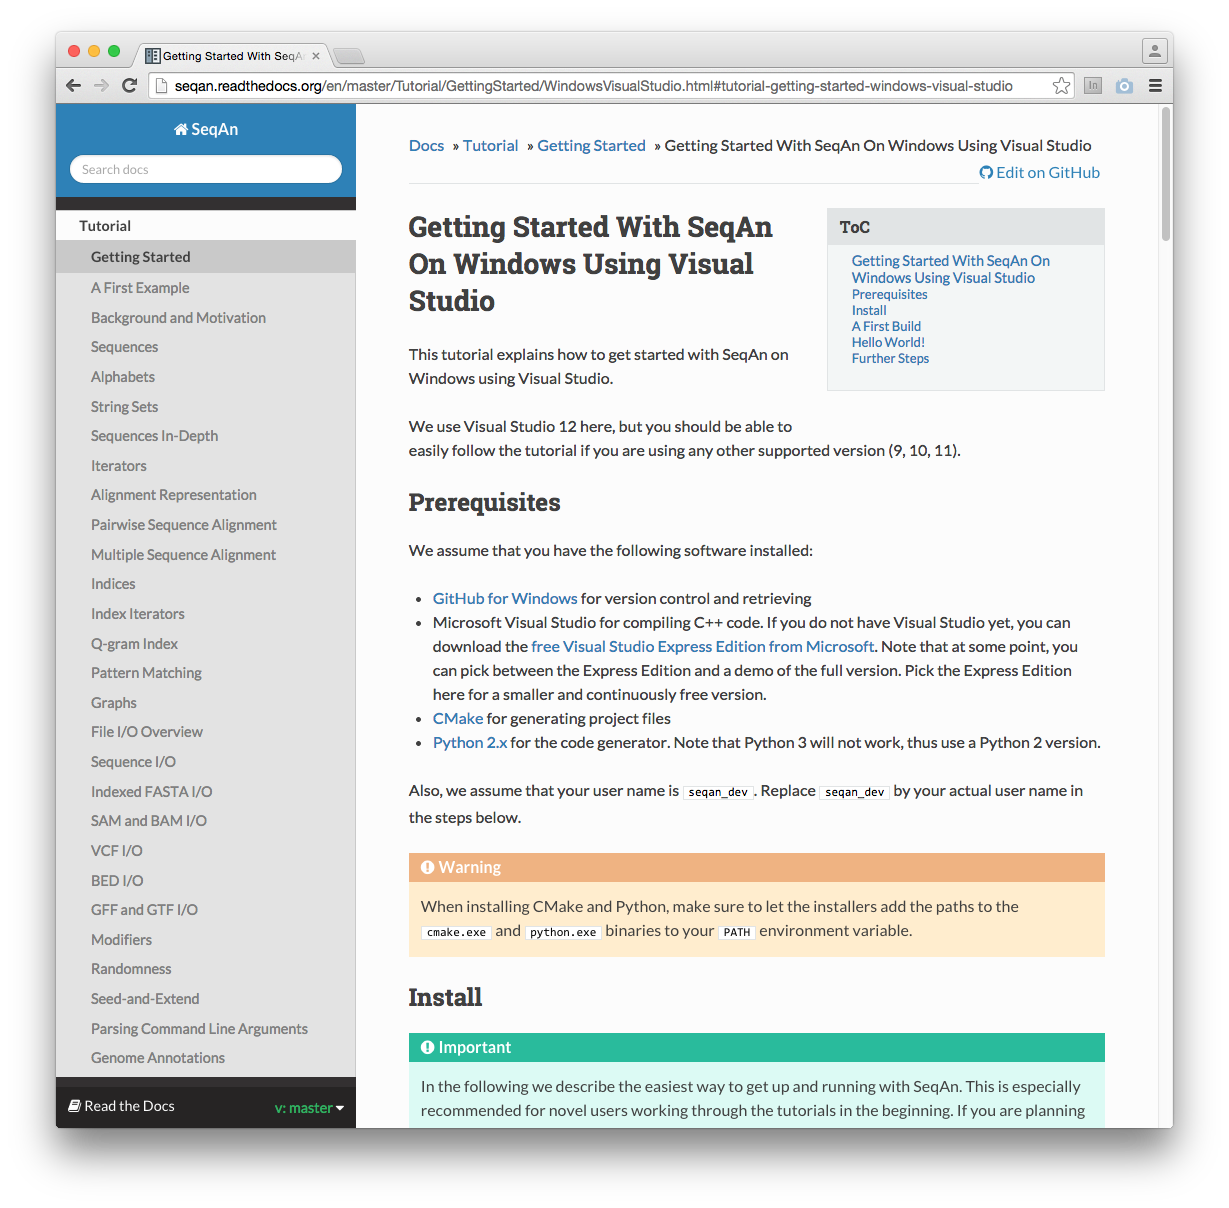
\includegraphics[width=1.0\linewidth]{Figures/getting-started-windows.png}
  \caption[SeqAn-Installation unter Windows]{Ausschnitt aus der verbesserten SeqAn-Installationsanleitung für Windows}
  \label{fig:getting-started-windows2}
\end{figure}



\subsubsection{Tutorials}

Basierend auf dem etablierten Lernphasenmodell \citep{Gagne:1985tx} und den Analyseergebnissen einer Vielzahl von Daten (Details siehe \sref{sec:phase1}) habe ich die Struktur der Tutorials überarbeitet und Qualitätskriterien formuliert. Diese Ergebnisse habe ich in Form eines Tutorials über das Schreiben von Tutorials zusammengefasst und in die Entwickler-Dokumentation integriert\footnote{\url{http://seqan.readthedocs.org/en/master/HowTo/WriteTutorials.html}}. Das Dokument richtet sich an die Autoren von SeqAn-Tutorials, wurde von diesen sehr positiv aufgenommen, gilt seitdem als verbindliche Vorlage für neue Tutorials und stellt damit einen langfristigen Beitrag für die verbesserte API-Usability von SeqAn dar.

Das Dokument besteht aus den folgenden Abschnitten:
\begin{enumerate}
\itemsep1pt\parskip0pt\parsep0pt
  \item Konventionen, die beim Verfassen von Tutorials zu beachten sind
  \item Struktur --- Aufbau eines Tutorials, explizite Metaangaben
  \item Didaktik --- Anwenderzentrierung, Übungsaufgaben
  \item Integration --- Vernetzung des Tutorials für bessere Auffindbarkeit
  \item Vorlage --- für die Erstellung eines neuen Tutorials
\end{enumerate}

Es wurden mehrere neue Tutorials durch das Auftrennen existierender Tutorials geschaffen. Besonders erwähnenswert ist dabei das neue Anfänger-Tutorial ``A First Example''\footnote{\url{http://seqan.readthedocs.org/en/master/Tutorial/FirstStepsInSeqAn.html}}, das eine besonders geringe Einstiegshürde für Anwender mit den in der \gls{gtm}-Analyse gefundenen \code[apiua://code/-9223372036854775494]{paradigmatischen Prägungen} aufweist. Es lohnt sich für den Leser dieser Dissertation das Anfänger-Tutorial einmal selbst zu öffnen.

Die Tutorials wurden sukzessive über eine längere Diskussionsphase hinweg gemeinsam von mir und den jeweiligen Autoren verbessert (siehe \fref{fig:tutorial-improved-final}) und dienen fortan als Aufgaben-bezogener SeqAn-Überblick \citep[vgl.][]{Fairbanks:2006jw,Ko:2011vw,Pugh:Ks4cicwp,Robillard:2009cs}.

\begin{figure}[ht!]
  \centering
    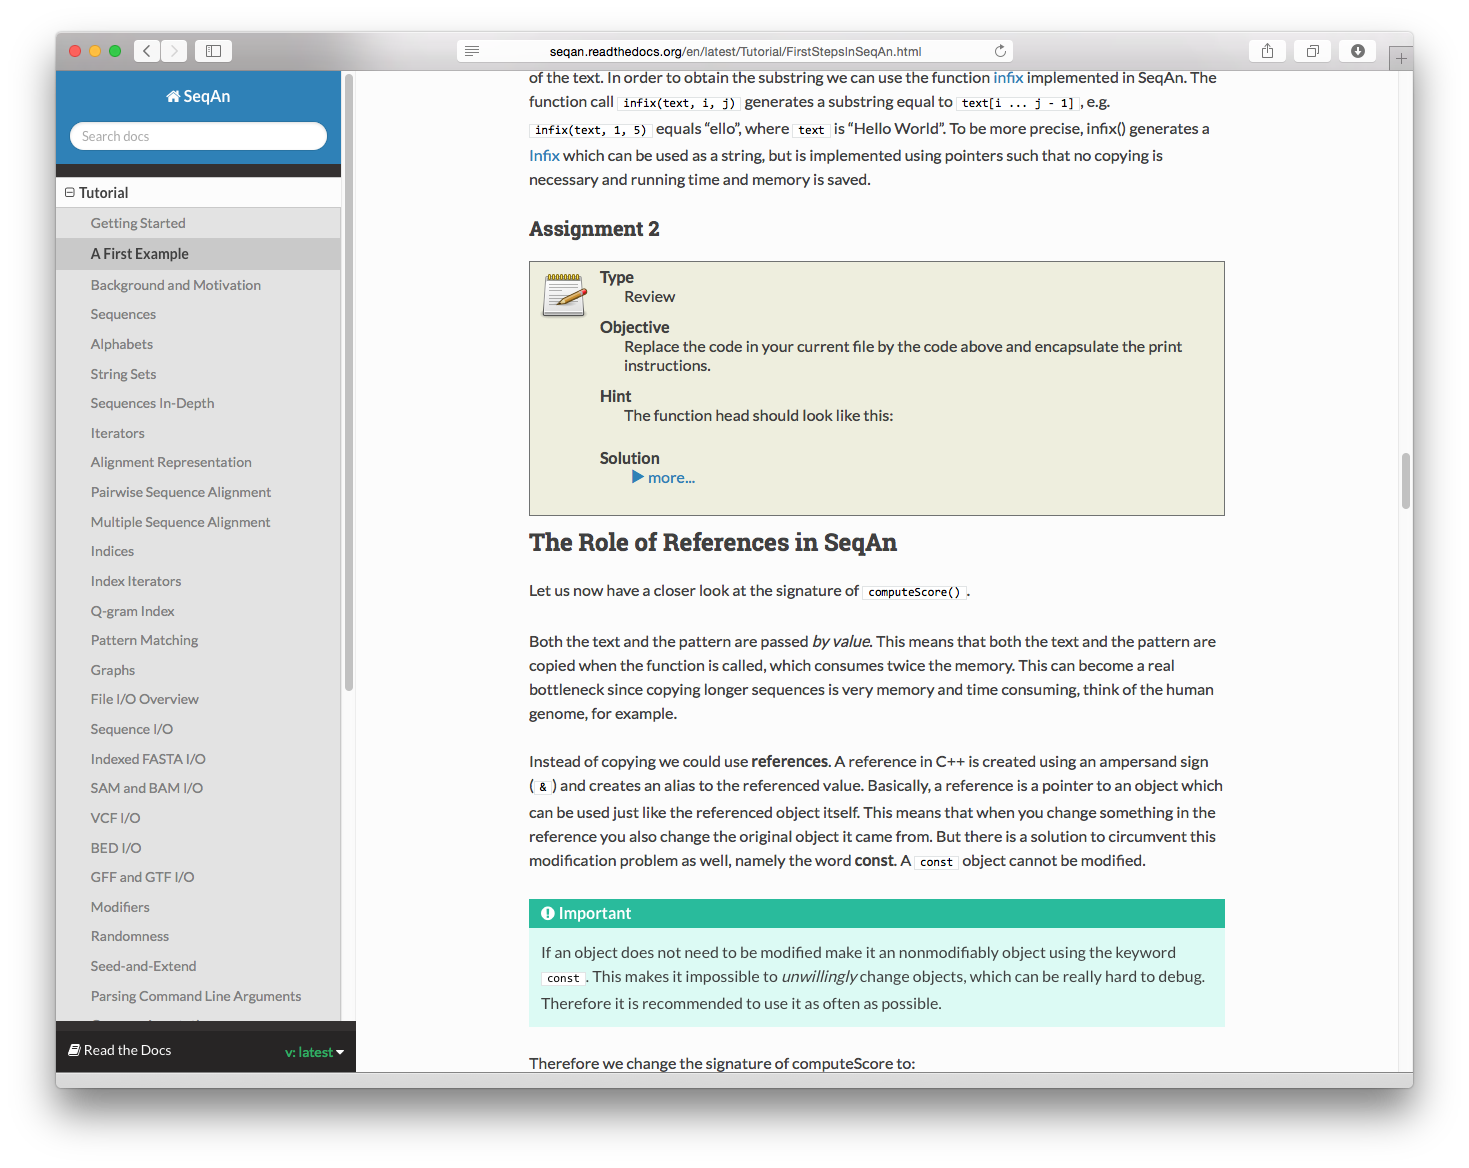
\includegraphics[width=1\linewidth]{Figures/tutorial-improved-final.png}
  \caption{Beispiel für ein überarbeitetes Tutorial}
  \label{fig:tutorial-improved-final}
\end{figure}




\subsubsection{Dokumentation}

Dokumentationen bilden ein wichtiges Bindeglied zwischen dem, was der Anwender möchte und dem, was die Library anbietet \citep{Robillard:2009cs,Kintsch:1988bz,Pennington:1987dc}. Aus diesem Grund und meinen \gls{gtm}-Analyseergebnissen habe ich die eigentliche SeqAn-Dokumentation technisch von Grund auf neu entwickelt. Die inhaltliche Überarbeitung wurde von den SeqAn-Entwicklern durchgeführt. Die \fref{fig:dox-large-all} zeigt die alte und die neue Dokumentation im Vergleich. Alternativ bietet es sich an, während des Lesens dieses Abschnitts die Dokumentation unter \href{http://docs.seqan.de/seqan/develop/}{docs.seqan.de/seqan/develop/} selbst zu öffnen.

Im Folgenden erläutere ich die Änderungen gegenüber der alten Dokumentation.

\newgeometry{inner=2cm,outer=1.5cm,top=1.5cm,bottom=1.5cm}
\thispagestyle{empty}
\begin{landscape}
\begin{figure}
        \centering
        \begin{subfigure}[b]{0.38\linewidth}
                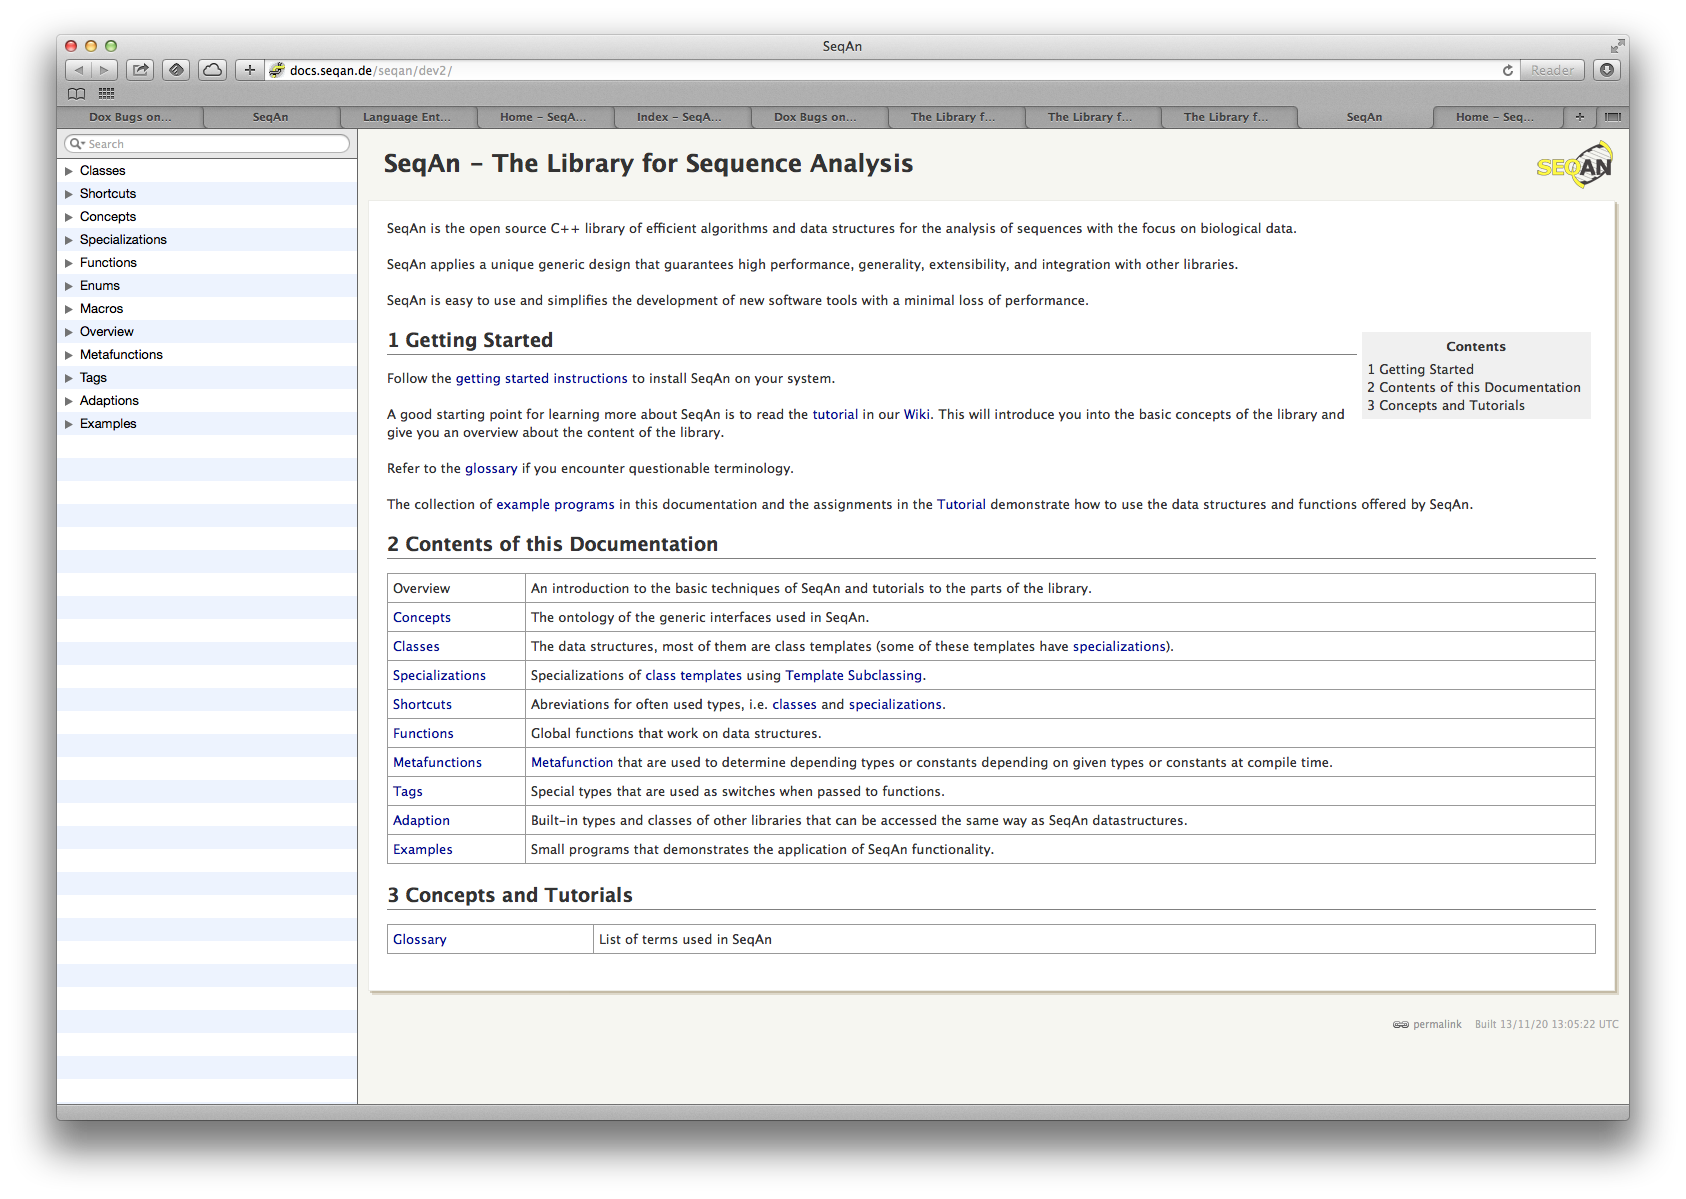
\includegraphics[width=\linewidth]{Figures/dox/dox-2_0_0-large-home.png}
                \caption{Startseite in Version 2.0.0}
                \label{fig:dox-large-home-2.0.0}
        \end{subfigure}
        \hspace{1cm}
        \begin{subfigure}[b]{0.38\linewidth}
                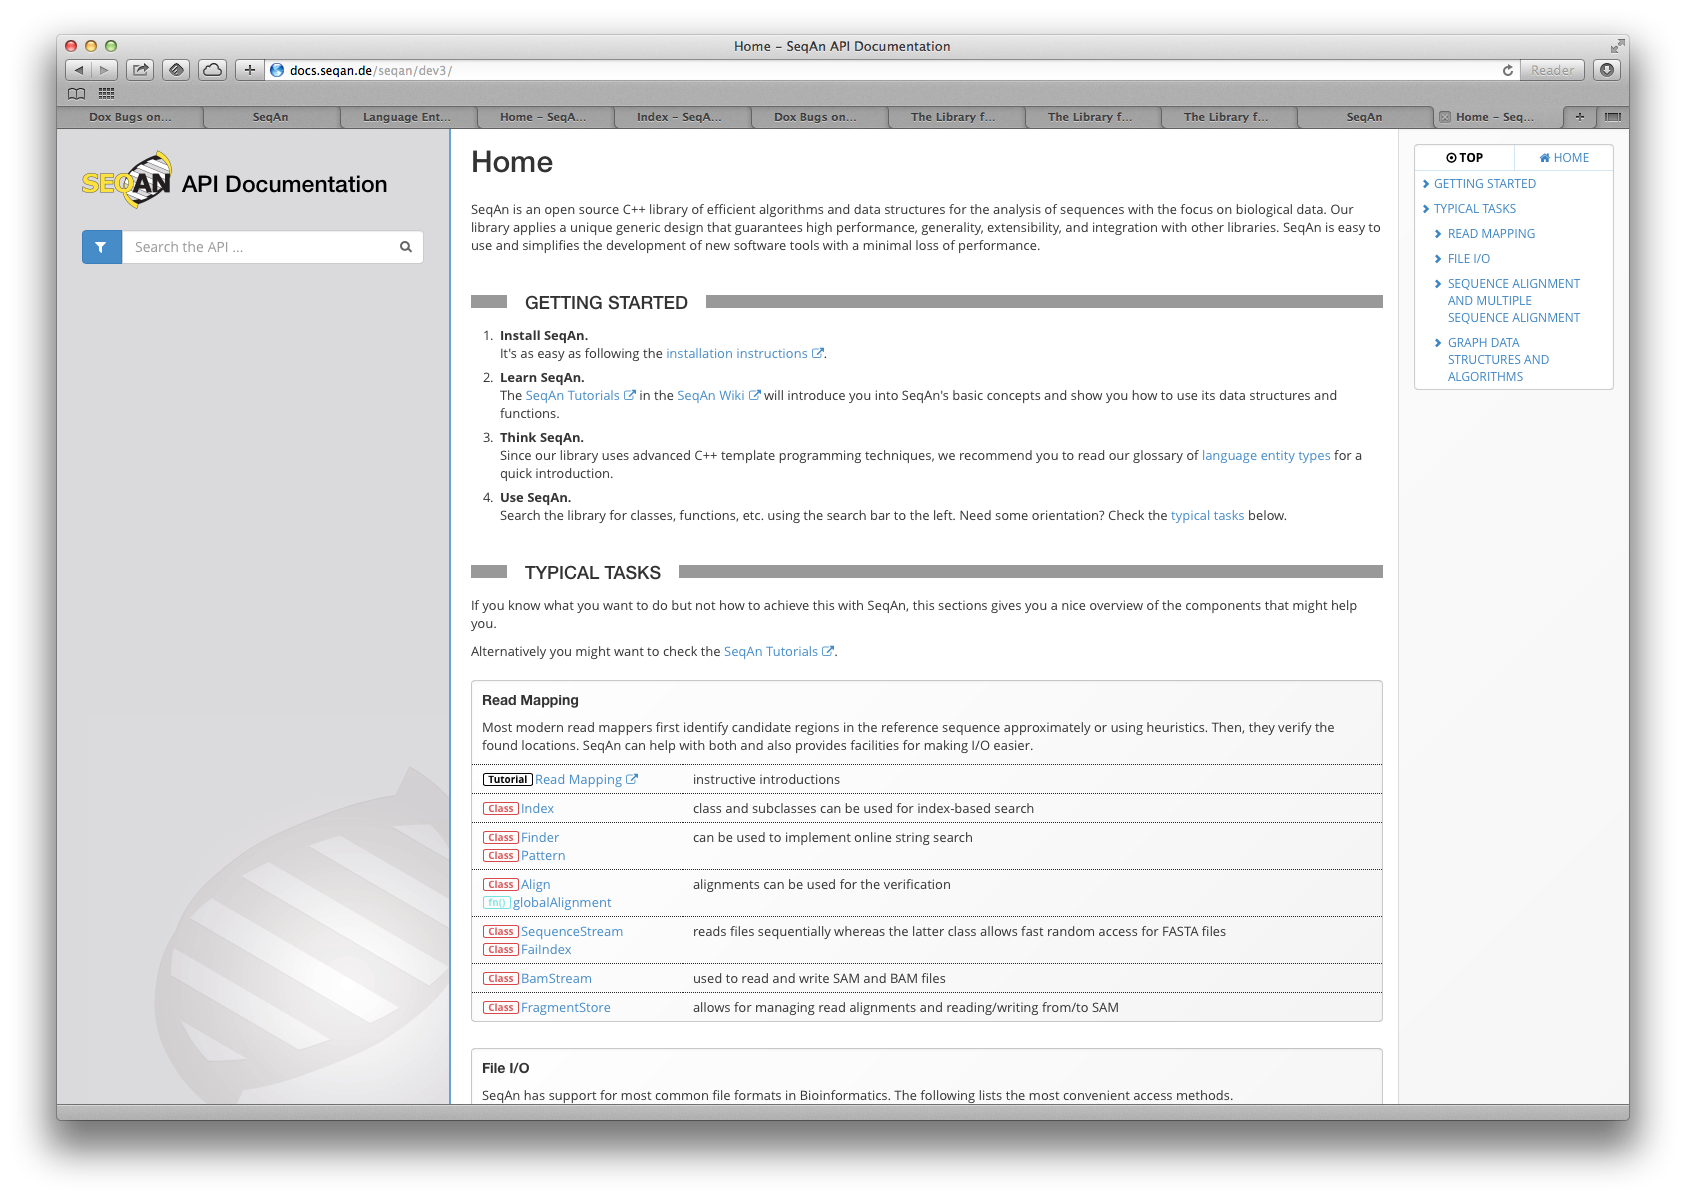
\includegraphics[width=\linewidth]{Figures/dox/dox-3_0_0-large-home.png}
                \caption{Startseite in Version 3.0.0}
                \label{fig:dox-large-home-3.0.0}
        \end{subfigure}%
        \vskip\baselineskip
        \begin{subfigure}[b]{0.38\linewidth}
                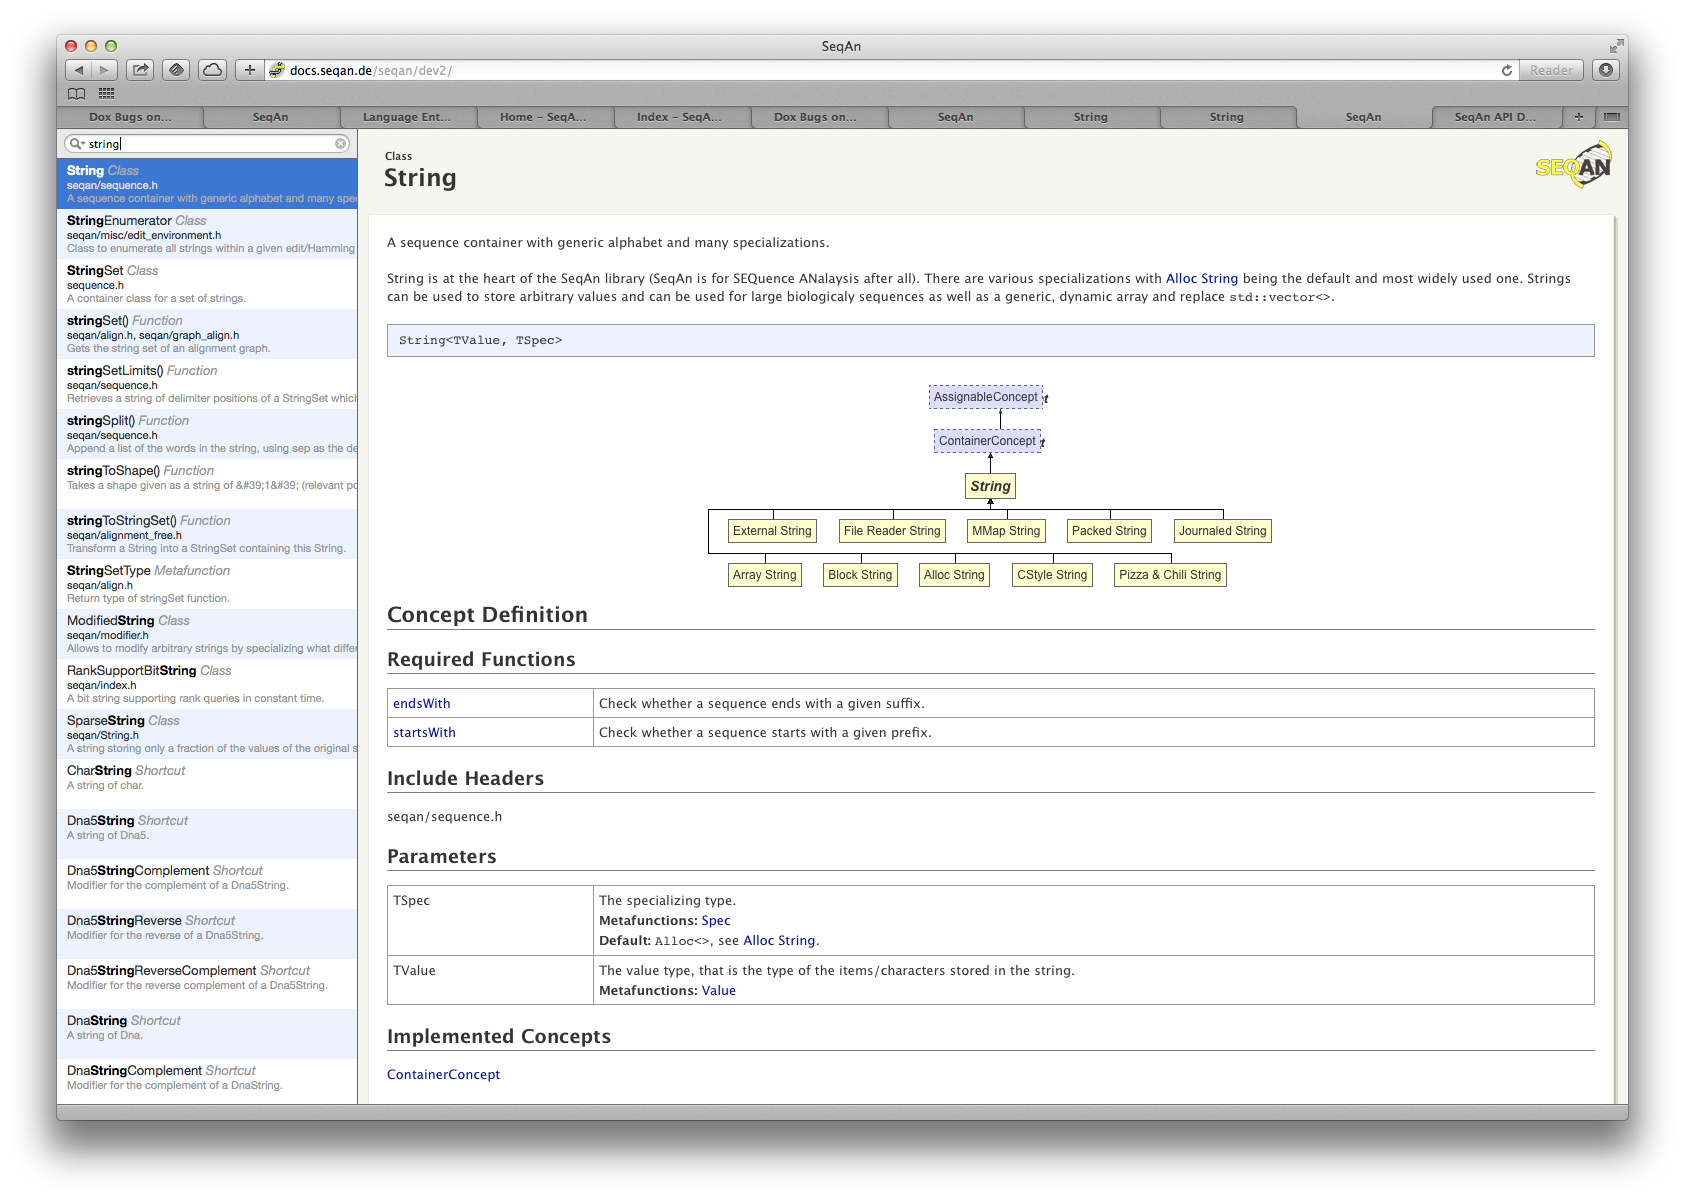
\includegraphics[width=\linewidth]{Figures/dox/dox-2_0_0-large-string-opened.png}
                \caption{Geöffnete \texttt{String}-Klasse in Version 2.0.0}
                \label{fig:dox-large-string-opened-2.0.0}
        \end{subfigure}
        \hspace{1cm}
        \begin{subfigure}[b]{0.38\linewidth}
                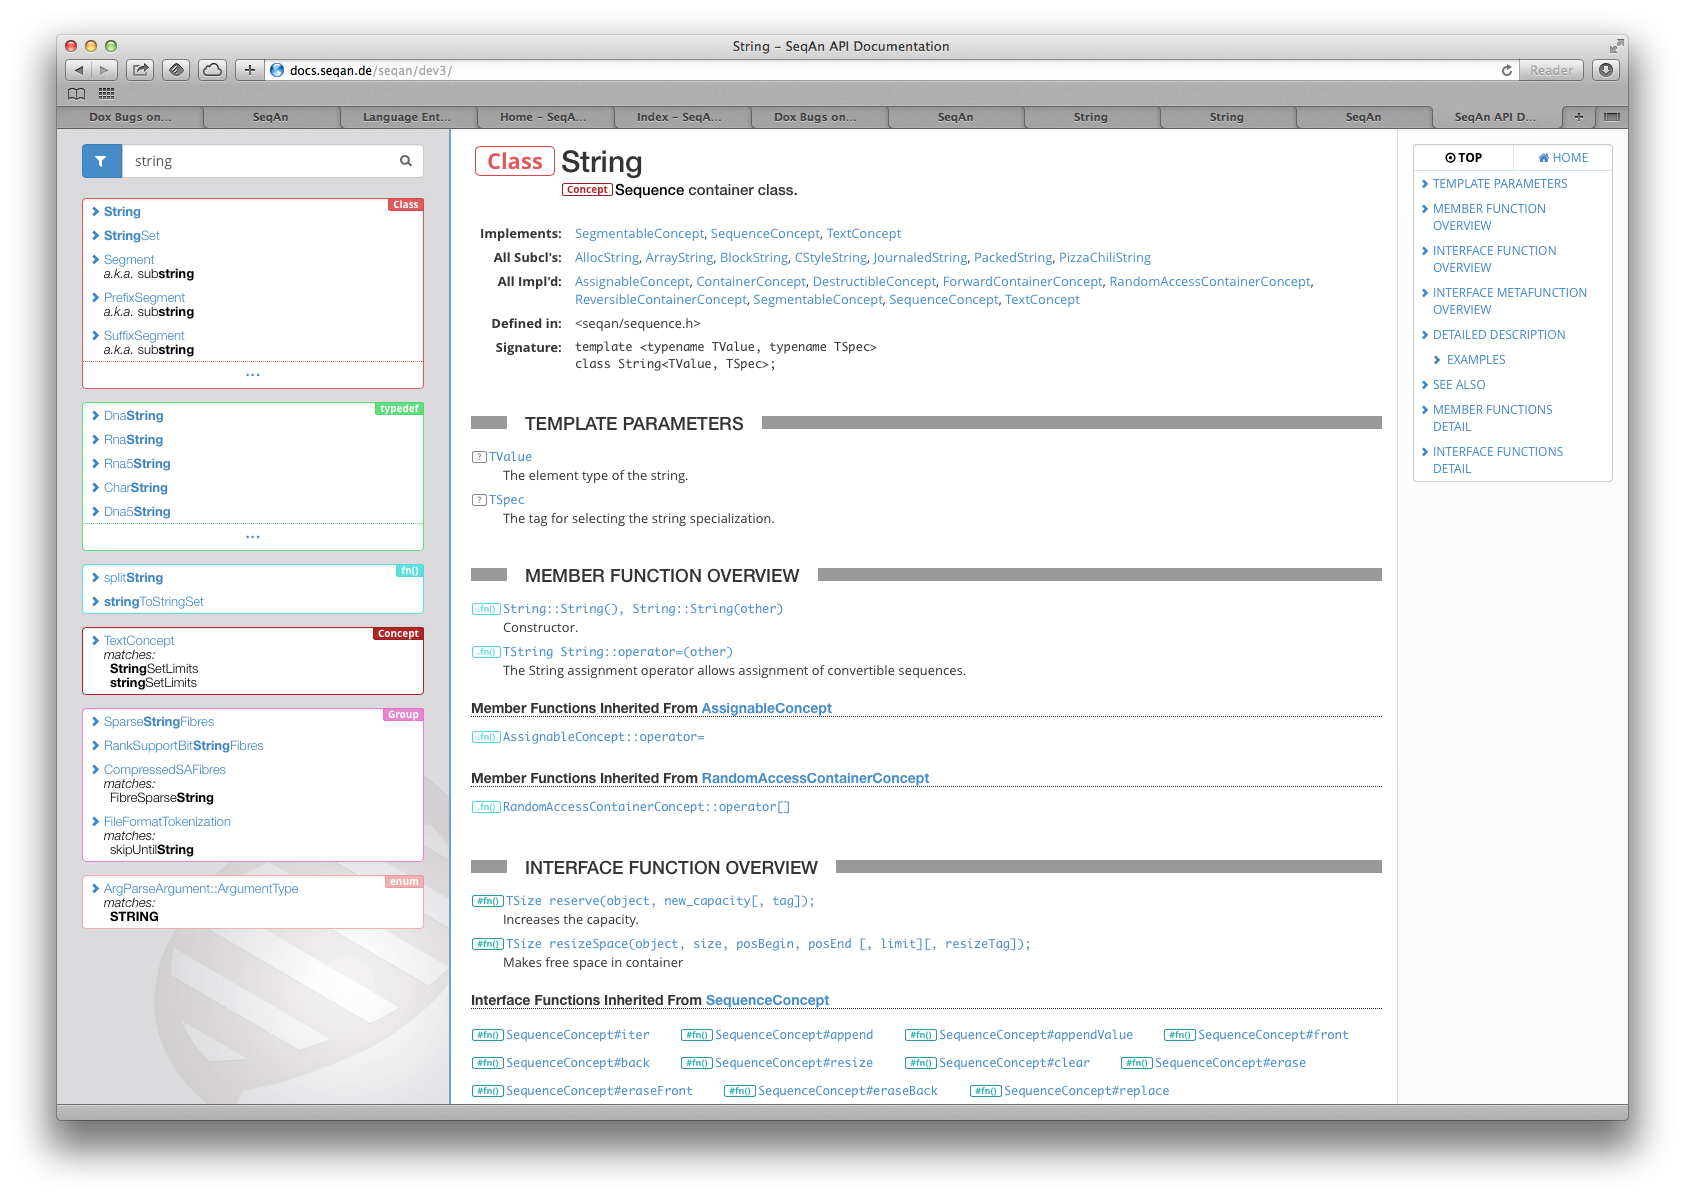
\includegraphics[width=\linewidth]{Figures/dox/dox-3_0_0-large-string-opened.png}
                \caption{Geöffnete \texttt{String}-Klasse in Version 3.0.0}
                \label{fig:dox-large-string-opened-3.0.0}
        \end{subfigure}
        \caption[Alte und neue Dokumentation im Vergleich --- in normaler Breite]{Die Abbildungen zeigen die alte und neue Dokumentation.}
        \label{fig:dox-large-all}
\end{figure}
\end{landscape}
\restoregeometry










\paragraph{Dokumentationssystem}

In Vorbereitung auf die technische Neuentwicklung der Dokumentation haben meine Kollegen und ich zunächst das in SeqAn verwendete Dokumentationssystem überarbeitet.

Der SeqAn-Entwickler Gogol Döring entwarf das \code[apiua://code/-9223372036854774817]{Dokumentationssystem} \textit{DDDoc} im Zuge einer \textit{expliziten-argumentativen} \code{apiua://code/-9223372036854775281}. Notwendig war (und ist) ein selbst entwickeltes Dokumentationssystem, da SeqAn, die noch nicht in den C\texttt{++}-Sprachstandard aufgenommene Sprachentität \textit{Concept} verwendet.\footnote{Gogol-Dörings Einschätzung, dass Concepts unbedingt Bestandteil der Dokumentation sein müssen, konnte ich empirisch bestätigen. Wie die Probleme \code{apiua://code/-9223372036854775280} und \code{apiua://code/-9223372036854775544} zeigen, können ohne Concepts die inhaltliche Zusammengehörigkeit technisch global implementierter \mbox{(Meta-)Funktionen} vom Anwender nicht erkannt werden. Tatsächlich handelt es sich nämlich bei den meisten globalen Funktionen inhaltlich um \mbox{Interface-(Meta-)Funktionen.}}

Wie das folgende kleine Beispiel zeigt, unterscheidet sich DDDoc von bekannten Dokumentationssystemen wie JavaDoc oder Doxygen, indem es ungewöhnlich zu lesen und zu schreiben ist.

\begin{center}
\begin{minted}[linenos=false, firstnumber=1]{cpp}
/**
.Spec.SimpleScore
..general:Class.Score
..summary:Basic scoring scheme.
..description:
This class allows to do alignments with simple match/mismatch-based scores.
..remarks:This class also supports different gap open and extension costs.
..include:seqan/score.h
*/
\end{minted}
\captionof{listing}{DDDoc-Beispiel für die Template-Spezialisierung \texttt{SimpleScore}}
\label{lst:dddoc}
\end{center}

\bigskip

Mit meinem Vorschlag, das Format zu überarbeiten, rannte ich bei den SeqAn-Entwicklern offene Türen ein. Eine Überarbeitung würde außerdem die Möglichkeit bieten, die in DDDoc fehlende Unterscheidung zwischen den Beziehungen ``wird von Funktion verwendet'' und ``ist Teil der Schnittstelle eines Typs'' zu beheben. Aus diesen Gründen wurde ein Doxygen-Derivat namens \textit{Dox} entwickelt, das auch Concepts und damit auch globale Funktionsinterfaces und Templatevererbung unterstützt. Implementiert wurde ebenso ein C{}\verb!++!-Parser.

Das folgende Beispiel zeigt denselben Dokumentationseintrag im neuen Dox-Format:

\begin{center}
\begin{minted}[linenos=false, firstnumber=1]{cpp}
/*!
 * @class SimpleScore
 * @extends Score
 * @summary Basic scoring scheme.
 *
 * @signature template <typename TValue>
 *            class Score<Tvalue, Simple>;
 *
 * This class allows to do alignments with simple match/mismatch-based 
 * scores.
 */
template <typename TValue>
class Score<TValue, Simple> {...};
\end{minted}
\captionof{listing}{Dox-Beispiel für die Template-Spezialisierung \texttt{SimpleScore}}
\label{lst:dox}
\end{center}

\bigskip

Wie man erkennen kann, ist das neue Doxygen-Format durch seine Ähnlichkeit zu JavaDoc und Doxygen leichter zu lesen und zu schreiben.

Das nächste und letzte Beispiel zeigt den Dokumentationseintrag für die technisch globale, aber inhaltlich zum \texttt{Score} gehörige Interface-Funktion \texttt{scoreGapOpen}:

\begin{center}
\begin{minted}[linenos, firstnumber=1]{cpp}
/*!
 * @fn Score#scoreGapOpen
 *
 * @signature TValue scoreGapOpen(sc);
 *
 * @return TValue The gap open score value for <tt>sc</tt>.
 *         Tvalue is the value type of <tt>sc</tt>.
 * @param sc The @link Score @endlink object to query.
 */
template <typename TValue, typename TSpec, typename TSeqHValue, typename TSeqVValue>
inline TValue
scoreGapOpen(...)
\end{minted}
\captionof{listing}{Dox-Beispiel für die zur Klasse \texttt{Score} gehörige Interface-Funktion \texttt{scoreGapOpen}}
\label{lst:dox2}
\end{center}

\bigskip

Über mehrere Monate haben die SeqAn-Entwickler sämtliche DDDoc-Einträge zu Dox-Einträgen umgewandelt. Beim Debuggen dieser Umwandlungen half u.a. ein in der neuen Dokumentation implementierter Entwicklermodus.



\paragraph{Entwicklermodus}

Für die neue Dokumentation habe ich einen Entwicklermodus entwickelt, der sich an die SeqAn-Entwickler richtet. Der Entwicklermodus kann bei geöffneter Dokumentation durch die Tastenkombination \texttt{Shift+Ctrl}\footnote{Zu beachten ist, dass der rechte Bereich, also nicht der Suchbereich, über den Fokus verfügen muss.} aktiviert werden und wurde von mir so implementiert, dass er um beliebige Funktionen erweitert werden kann. Aktuell unterstützt er SeqAn-Entwickler bei den folgenden Tätigkeiten:
\begin{itemize}
  \item SeqAn-Entwickler können für jeden Dokumentationseintrag den dazugehörigen Dox-Eintrag im Quellcode einblenden lassen (siehe \fref{fig:dox-devmode-dox}).
  \item Insbesondere für das Schreiben von Tutorials benötigen SeqAn-Entwickler den Link zu einem bestimmten Eintrag. Dieser kann nicht ohne Weiteres aus der Adresszeile entnommen werden. Einerseits verwendet die Dokumentation \textit{IFrames}\footnote{\url{https://www.w3.org/wiki/HTML/Elements/iframe}}. Andererseits gibt es den Bedarf, auch einen ganz bestimmten Untereintrag innerhalb eines Dokumentationseintrages zu verlinken. Im Entwicklermodus werden alle verlinkbaren Elemente hervorgehoben. Ein Klick auf eines dieser Elemente bringt einen modalen Dialog hervor, der alle Verlinkungsmöglichkeiten anzeigt und auf Wunsch in die Zwischenablage kopiert (siehe \fref{fig:dox-devmode-permalink}).
\end{itemize}

Der Entwicklermodus wurde von den SeqAn-Entwicklern sehr gut angenommen, was man leicht an den schnellen Beschwerden, im Falle von entdeckten Bugs, sehen konnte.

\begin{figure}[ht!]
  \centering
    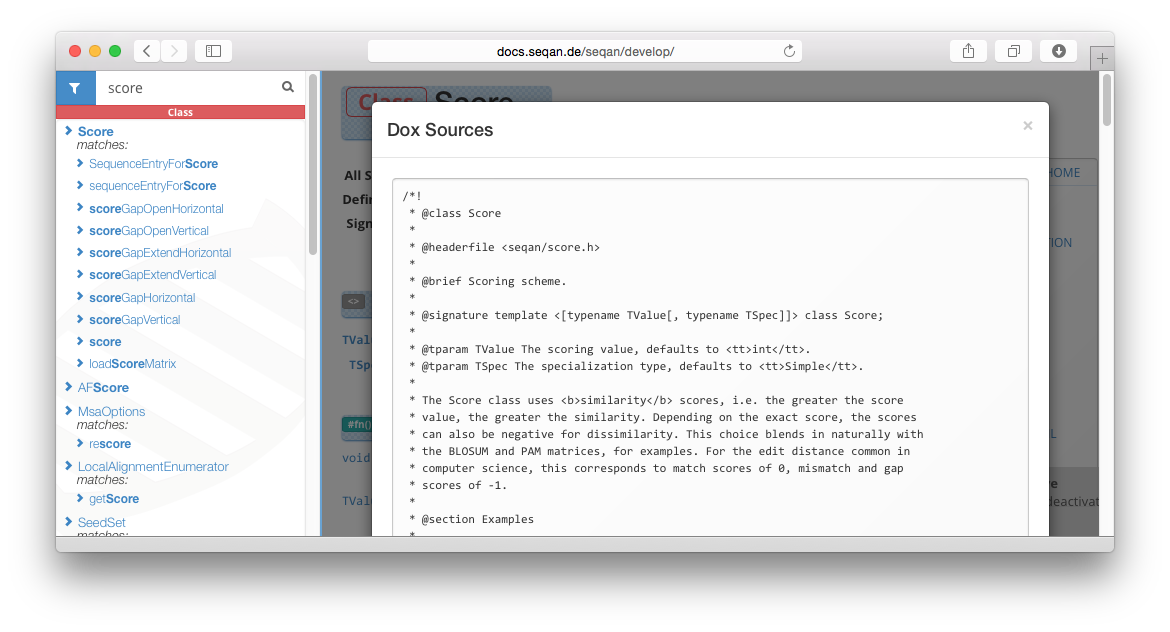
\includegraphics[width=0.9\linewidth]{Figures/dox/devmode-dox.png}
    \caption{Entwicklermodus --- Dox-Quelle für den aktuellen Dokumentationseintrag}
    \label{fig:dox-devmode-dox}
\end{figure}

\begin{figure}[ht!]
  \centering
    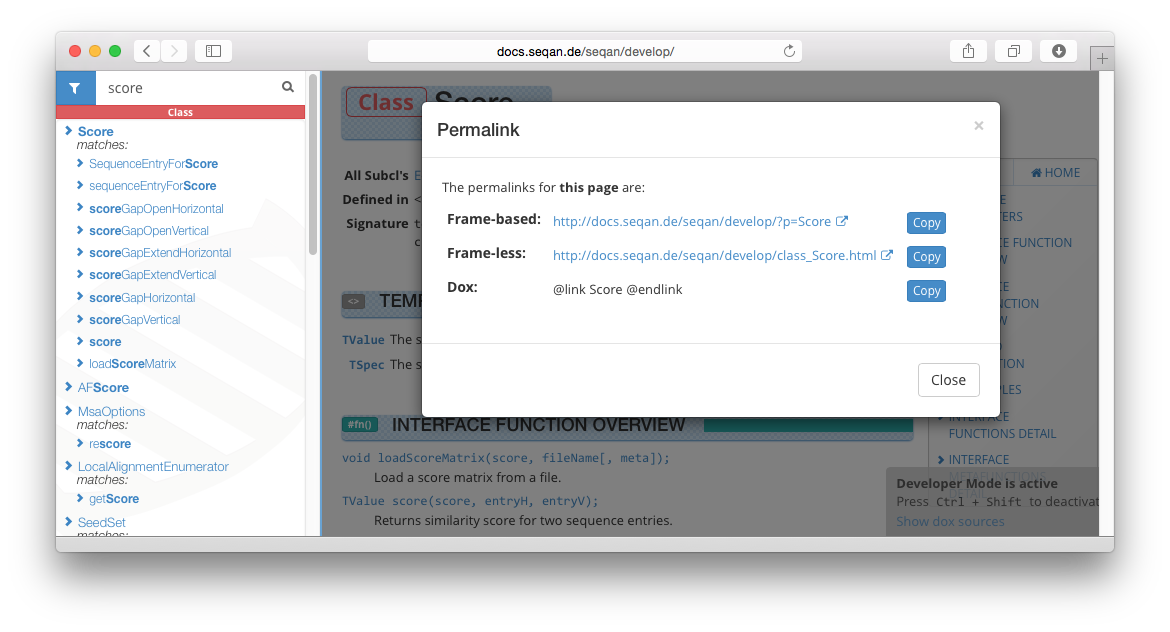
\includegraphics[width=0.9\linewidth]{Figures/dox/devmode-permalink.png}
    \caption[Entwicklermodus --- Anzeige aller Links für das aktuell selektierte Element]{Entwicklermodus: Anzeige aller Links für das aktuell selektierte Element. Im Hintergrund des modalen Dialogs kann man drei bläulich hinterlegte Elemente erkennen, die verlinkbar sind.}
    \label{fig:dox-devmode-permalink}
\end{figure}

%API-Entwickler müssen gute Dokumentation schreiben \citep{Kramer:1999ih}



\paragraph{Gesamtüberblick}

Die Notwendigkeit eines Gesamtüberblicks konnte ich empirisch zeigen und lässt sich auch direkt und indirekt aus der Literatur entnehmen. So verhindert ein fehlender Gesamtüberblick Top-Down-Lernen \citep[vgl.][]{Brooks:1983fj} und das Erkennen von Zusammengehörigkeit verteilter Informationen \citep[vgl.][]{BenShneiderman:gn} --- insbesondere für Anfänger \citep{Stylos:2008jt,Piccioni:2013uq}.

Werden an keiner Stelle Entwurfsentscheidungen gebündelt dargestellt, werden Anwender beim Anpassungen von Beispiel-Code eingeschränkt \citep{Bruch:2006bv}. Dies führt dazu, dass Anwender häufiger Fehler bei der Anpassung machen, und mit geringerer Wahrscheinlichkeit die korrekte Intention des Codes wiedergeben \citep{Fairbanks:2006jw}.

Außerdem muss die Startseite der Dokumentation über eine Aufgaben-bezogene, logische Gruppierung der Library-Elemente verfügen, da es klassenübergreifende Aufgaben gibt, deren Lösung sich für API-Anfänger sonst nicht ohne Weiteres erschließen würde. \citep{DaqingHou:2005ba,clarke:2006}

Die überarbeitete Startseite der SeqAn-Dokumentation verfügt nun über folgende Elemente:
\begin{itemize}\itemsep1pt\parskip0pt\parsep0pt
  \item Knappe Beschreibung von SeqAn
  \item \textit{Getting Started}
  \begin{itemize}
    \item Verweis auf die Installationsanleitungen
    \item Verweise auf die Tutorials und ähnliche Inhalte (Profiling, CMake, etc.)
    \item Verweis auf die Sprachentitätstypen-Übersichtseite
  \end{itemize}
  \item Typische SeqAn-Aufgaben mit Verweisungen auf die dazugehörigen Tutorials, Klassen und Funktionen. Die vier typischen Aufgaben lauten:
  \begin{itemize}
    \item Read-Mapping
    \item Ein- u. Ausgabe
    \item Sequence-Alignment
    \item Graphen
  \end{itemize}
\end{itemize}

Des Weiteren wurde das kaum auffindbare und veraltete Background-and-Motivation-Tutorial\footnote{\url{http://seqan.readthedocs.org/en/master/Tutorial/BackgroundAndMotivation.html}} umfassend überarbeitet. Es erklärt nun die Motivation der SeqAn zu Grunde liegenden Entwurfsentscheidungen und veranschaulicht den SeqAn-Performance-Gewinn an Hand eines ohne SeqAn geschriebenen Beispiels.

%High-level Design-Dokumentation notwendig \citep{Robillard:2009cs}
%Globale Designentscheidungen müssen auf Startseite der Doku erklärt werden \citep{Robillard:2009cs}




\paragraph{Sprachentitätstypen}

Das Konzept der \code{apiua://code/-9223372036854775413} (engl. \textit{language entity types}) ist in SeqAn von besonders großer Relevanz, da SeqAn durch den Gebrauch von Concepts Sprachentitätstypen verwendet, die dem Gros der SeqAn-Anwender unbekannt sind (siehe \sref{sec:gt-let}). Dabei ist es von elementarer Wichtigkeit, bedeutende Konzepte in einer Dokumentation zu erklären \citep{Jeong:kf,Ko:2011vw,Monperrus:2011bf}.

Mein Ziel war es, Anwender unaufdringlich auf die Existenz neuer Sprachentitätstypen hinzuweisen und es ihnen zu erlauben, sich auf leichtgewichtige Art darüber zu informieren. Dieser Ansatz wird als \textit{knowledge pushing} bezeichnet und wurde bereits in ähnlicher Weise von \cite{Watson:2009da,sunshine2014searching} erfolgreich angewendet.

Die Umsetzung erfolgte wie folgt:
\begin{itemize}
  \item Alle in der Dokumentation genannten Sprachentitäten, wie \texttt{length} oder \texttt{String}, werden durch ein kleines Label annotiert.
  \item Jedes Label kennzeichnet einen Sprachentitätstyp.
  \item Die Labels werden durch zwei Merkmale unterschieden:
  \begin{enumerate}
    \item Farbe, welche die Zusammengehörigkeit verschiedener Sprachentitätstypen symbolisiert.
    \item Ideogramm, also ein textuelles Piktogramm, das den Sprachentitätstyp phänotypisch ausdrückt.
  \end{enumerate}
  \item Die existierenden Sprachentitätstypen lauten:
  \begin{itemize}
    \item[] \raisebox{-0.4ex}{
\includegraphics[height=1em]{Figures/lets/typedef.png}} Typdefinition mittels \texttt{typedef}
    \hspace{1em} \raisebox{-0.4ex}{
\includegraphics[height=1em]{Figures/lets/variable.png}} Variable\footnote{Beim Schreiben dieser Dissertation wurde mir klar, dass \textit{var} ein geeigneteres Ideogramm darstellt. Ein entsprechender Issue-Tracker-Eintrag existiert: \url{https://github.com/seqan/seqan/issues/1034}}
    
    \item[] \raisebox{-0.4ex}{
\includegraphics[height=1em]{Figures/lets/concept.png}} Concept
    \hspace{1em} \raisebox{-0.4ex}{
\includegraphics[height=1em]{Figures/lets/class.png}} Klasse
    \hspace{1em} \raisebox{-0.4ex}{
\includegraphics[height=1em]{Figures/lets/spec.png}} Spezialisierung
    \hspace{1em} \raisebox{-0.4ex}{
\includegraphics[height=1em]{Figures/lets/enum.png}} Enum
    
    \item[] \raisebox{-0.4ex}{
\includegraphics[height=1em]{Figures/lets/globalmetafunction.png}} Globale Metafunktion
    \hspace{1em} \raisebox{-0.4ex}{
\includegraphics[height=1em]{Figures/lets/interfacemetafunction.png}} Interface-Metafunktion
    \hspace{1em} \raisebox{-0.4ex}{
\includegraphics[height=1em]{Figures/lets/tag.png}} Tag
    
    \item[] \raisebox{-0.4ex}{
\includegraphics[height=1em]{Figures/lets/globalfunction.png}} Globale Funktion
    \hspace{1em} \raisebox{-0.4ex}{
\includegraphics[height=1em]{Figures/lets/interfacefunction.png}} Interface-Funktion
    \hspace{1em} \raisebox{-0.4ex}{
\includegraphics[height=1em]{Figures/lets/memberfunction.png}} Member-Funktion

    \item[] \raisebox{-0.4ex}{
\includegraphics[height=1em]{Figures/lets/adaption.png}} Adaption
    \hspace{1em} \raisebox{-0.4ex}{
\includegraphics[height=1em]{Figures/lets/makro.png}} Makro
  \end{itemize}
  \item Bewegt der Anwender die Maus über ein Label, wird eine minimale Beschreibung des dazugehörigen Sprachentitättyps eingeblendet (siehe \fref{fig:dox-let-hover}).
  \item Klickt der Anwender bei eingeblendeter minimaler Beschreibung auf das Label, wird die ausführlichere Beschreibung des Sprachentitättyps geöffnet (siehe \fref{fig:dox-let-detail}).
  \item Sowohl Suchergebnisse als auch Funktionsauflistungen innerhalb von Dokumentationseinträgen sind nach den Sprachentitätstypen gruppiert (siehe \fref{fig:dox-large-string-opened-3.0.0}).
  \item Die Suchfunktion der Dokumentation erlaubt die Filterung der Ergebnisse nach Sprachentitätstypen. Tatsächlich ging es mir aber nicht um die Funktion selbst, sondern darum, dass neugierige Anwender so auf eine vollständige Auflistung der in SeqAn präsenten Sprachentitätstypen stoßen, ohne sich mit diesen gleich aktiv auseinandersetzen zu müssen.
\end{itemize}

\begin{figure}[ht!]
  \centering
    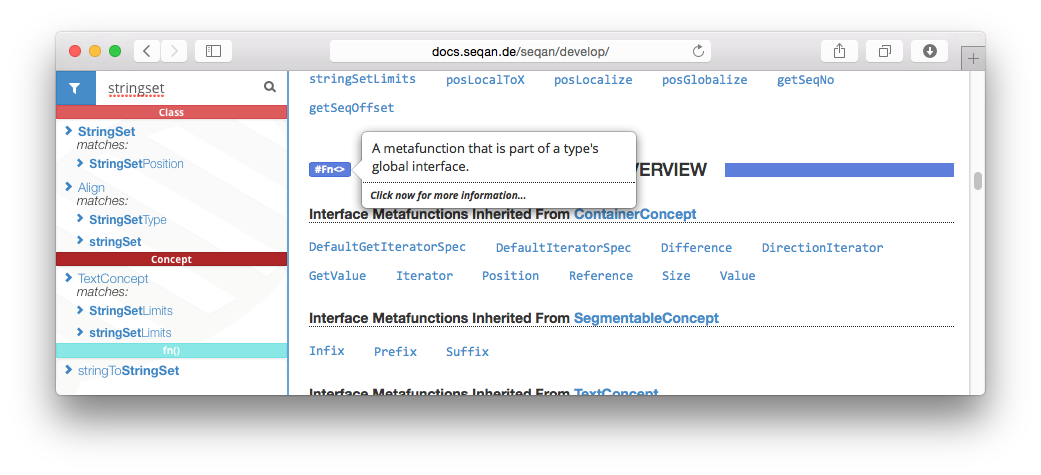
\includegraphics[width=0.9\linewidth]{Figures/dox/let-hover.png}
    \caption{Kurzbeschreibung des Sprachentitättyps \textit{Interface-Metafunktion}}
    \label{fig:dox-let-hover}
\end{figure}

\begin{figure}[ht!]
  \centering
    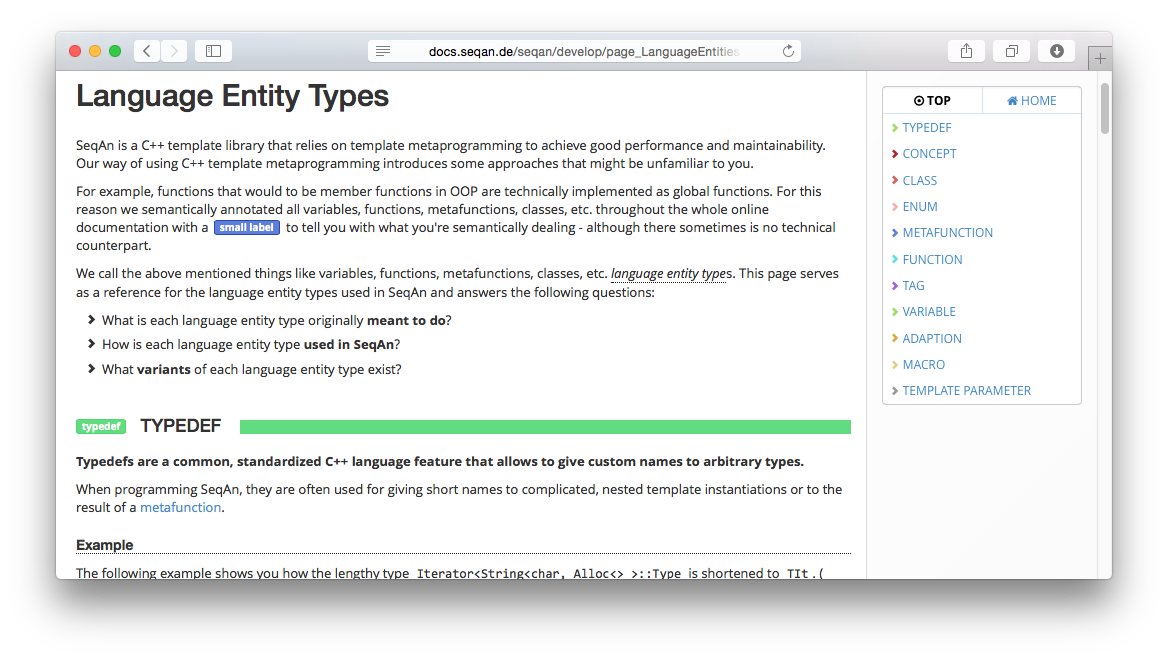
\includegraphics[width=0.9\linewidth]{Figures/dox/let-detail.png}
    \caption{Ausführliche Beschreibung der in SeqAn verwendeten Sprachentitätstypen}
    \label{fig:dox-let-detail}
\end{figure}



\paragraph{Seitenaufbau}

Der Aufbau von Dokumentationsseiten wurde von mir und einem SeqAn-Entwickler überarbeitet. Abstrakt sind Seiten wie folgt gegliedert:
\begin{enumerate}
\itemsep1pt\parskip0pt\parsep0pt
  \item Zusammenfassung zum Nachschlagen
  \item Detaillierte Beschreibung
\end{enumerate}

Im Grunde gibt es zwei Seitentypen:
\begin{description}
  \item[Containerseiten] kommen zur Dokumentation von Concepts, Klassen und Spezialisierungen zum Einsatz\footnote{Beispiel String-Klasse: \url{http://docs.seqan.de/seqan/develop/?p=String}}, da diese Sprachentitätstypen über Untereinträge verfügen. Hierbei umfasst die Zusammenfassung einen Bereich für Metainformationen und eine Auflistung aller verfügbaren Funktionen. Die Metainformationen zählen bei Klassen beispielsweise auf, welche Concepts direkt und indirekt implementiert werden, welche Spezialisierungen existieren, in welcher Datei die Klasse definiert ist und welche Signatur die Klasse besitzt. Die Auflistung der Funktionen ist gegliedert nach Member-Funktionen, Interface-Funktionen und Interface-Metafunktionen. Der Detailbereich erläutert im Falle einer Klasse den Gebrauch der Klasse samt Beispielen und erklärt detailliert sämtliche oben genannten Funktionen im Detail.
  \item[Elementseiten] sind atomar und kommen für alle anderen Sprachentitätstypen zum Einsatz\footnote{Beispiel globalAlignment-Funktion: \url{http://docs.seqan.de/seqan/develop/?p=globalAlignment}}, da diese über keine Untereinträge verfügen. Im Falle von (semantisch) globalen Funktionen umfasst die Zusammenfassung eine Auflistung aller Parameter und die Beschreibung der Rückgaben. Der Detailbereich erläutert dann wiederum ausführlich Sinn und Zweck der Funktion und beschreibt dies an Hand von Beispielen.
\end{description}

In SeqAn werden häufig Referenzen technisch als Eingaben übergeben, inhaltlich aber als Rückgaben behandelt. Ob ein Parameter als Ein- und/oder Ausgabe behandelt wird, wird durch die folgenden Icons ausgezeichnet: 
\includegraphics[height=.7em]{Figures/dox/in.png}, 
\includegraphics[height=.7em]{Figures/dox/out.png} und 
\includegraphics[height=.7em]{Figures/dox/inout.png}.


\paragraph{Beispiele}

Beispiele sind neben der Gesamtübersicht der wichtigste Bestandteil einer benutzerfreundlichen Dokumentation \citep{Robillard:2010bh}, was ich an Hand der verschiedenen, durch die Abwesenheit (guter) Beispiele eingeschränkten Beispiel-bezogenen Strategien empirisch belegen konnte (siehe \sref{sec:dox}).

Im Zuge der inhaltlichen Überarbeitung der Dokumentation wurden für die wichtigsten Dokumentationseinträge existierende Beispiele verbessert und fehlende Beispiele ergänzt. Dabei wurden alle Beispiele um die Programmausgabe ergänzt, was besonders für API-Endanwender wichtig ist \citep{Gross:2010iz}.



\paragraph{Suchfunktion}

Die vollständig neu entwickelte Suchfunktion verfügt über die folgenden Funktionen:
\begin{itemize}
  \item Sprachentitäten können nun über Aliasse/Synonyme verfügen. Auf diese Weise wurden die im \textit{Vocabulary Problem} \citep{Furnas:1987hl} veranlagten Usability-Probleme gemildert. Der Suchbegriff \texttt{substring} beispielweise führt nun auch zu dem Treffer \textit{infix}. Wurde ein Eintrag mit Hilfe eines Synonyms gefunden, wird dem Anwender dies mitgeteilt. Auf diese Weise lernt der Anwender bedarfsgerecht die korrekte Bezeichnung in SeqAn. Anwender, die ohnehin den korrekten Begriff verwendet haben, erfahren nicht von den Synonymen. Auf diese Weise wird verhindert, dass unterschiedlich benannte, aber inhaltlich identische Sprachentitäten innerhalb von SeqAn gepflegt werden müssen.
  \item Die Suchergebnisse sind nun gewichtet, so dass beispielsweise der Suchbegriff \texttt{string} auch tatsächlich die \texttt{String}-Klasse als ersten Suchtreffer hervorbringt.
  \item Die Suchergebnisse sind nach Sprachentitätstypen gruppiert und auf maximal fünf Einträge je Typ begrenzt. Auslassungspunkte am Ende einer Treffergruppe deuten darauf hin. Ein Klick darauf zeigt alle Suchtreffer der Gruppe.
  \item Suchergebnisse können auch Dokumentationsteileinträge sein. So ist der erste Suchtreffer für \texttt{infix}, die \texttt{Infix}-Interface-Metafunktion innerhalb des Concepts \texttt{SegmentableConcept}. Der Anwender kann selbst wählen, ob der den Dokumentationseintrag oder -untereintrag öffnen möchte.
  \item Die Suche kann ohne Maus und ausschließlich mit der Tastatur bedient werden. Dazu erhält das Suchfeld automatisch den Fokus, die Sucheingabe kann mit \texttt{Esc} gelöscht und innerhalb der Suchergebnisse mit den Pfeiltasten navigiert werden.
\end{itemize}

  



\paragraph{Darstellung}

Die Online-Dokumentation ist \textit{responsive}\footnote{\url{https://developers.google.com/web/fundamentals/layouts/rwd-fundamentals/}}, passt sich also einer großen Bandbreite von Fenstergrößen an. Dies ist nicht nur schick, sondern auch hilfreich. Bei SeqAn-Anfängern konnte ich einen häufigen Wechsel zwischen Entwicklungsumgebung und Online-Dokumentation beobachten. Da die neue SeqAn-Dokumentation selbst bei einem 600 Pixel schmalen Fenster (bei 72 DPI) ohne Einschränkung nutzbar ist, können SeqAn-Anwender die Dokumentation auch neben der Entwicklungsumgebung platzieren. Auch ist eine Nutzung der Dokumentation auf mobilen Geräten möglich, wie es einige Anwender forderten.

Des Weiteren habe ich großen Wert auf eine hohe Ästhetik gelegt. Ich denke, dieses u.a. durch den Einsatz von subtilen Farbverläufen und dezenten Animationen erreicht zu haben. Spaß an der Bedienung ist ein wesentlicher Aspekt des Anwendererlebnisses und spielt damit auch für SeqAns kommerziellen Erfolg eine Rolle.

\fref{fig:dox-small-all} stellt die gleichen Inhalte wie \fref{fig:dox-large-all} auf Seite \pageref{fig:dox-large-all} dar --- nur mit dem Unterschied eines schmaleren Browser-Fensters.

\newgeometry{inner=2cm,outer=1cm,top=1.5cm,bottom=1.5cm}
\thispagestyle{empty}
%\begin{landscape}
\begin{figure}
        \centering
        \begin{subfigure}[b]{0.48\linewidth}
                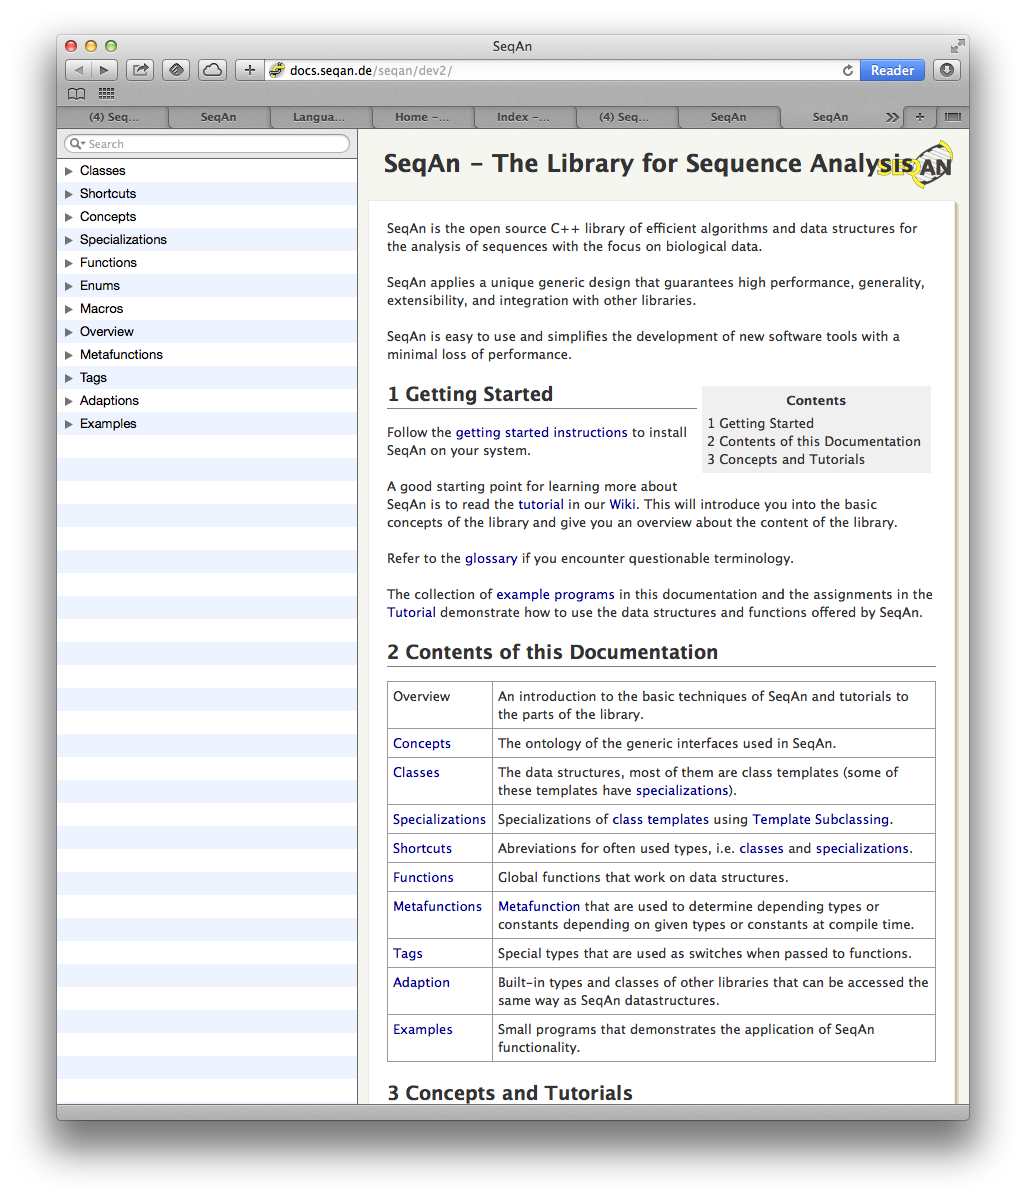
\includegraphics[width=\linewidth]{Figures/dox/dox-2_0_0-small-home.png}
                \caption{Startseite in Version 2.0.0}
                \label{fig:dox-small-home-2.0.0}
        \end{subfigure}
        \hfill
        \begin{subfigure}[b]{0.48\linewidth}
                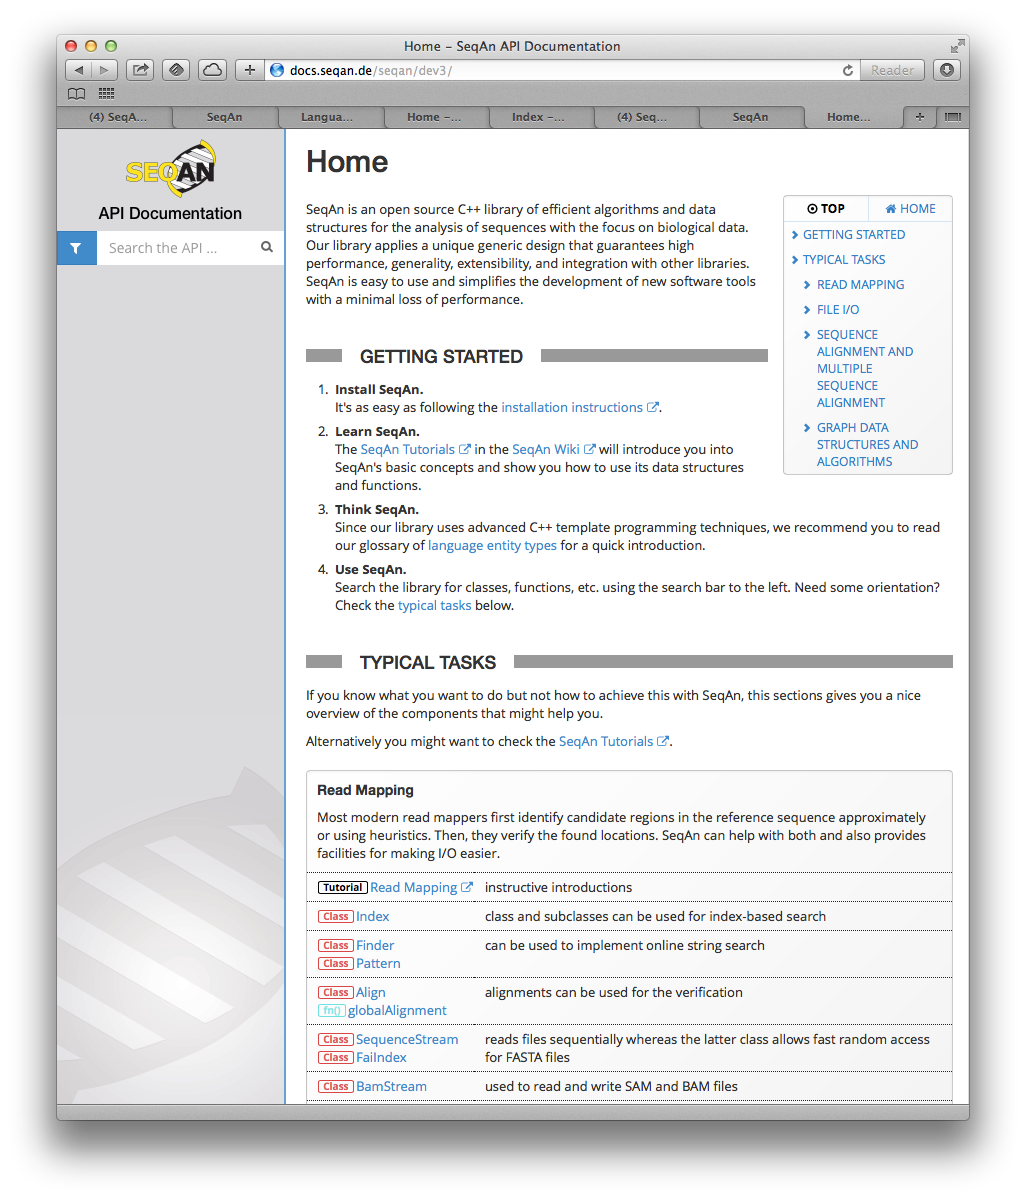
\includegraphics[width=\linewidth]{Figures/dox/dox-3_0_0-small-home.png}
                \caption{Startseite in Version 3.0.0}
                \label{fig:dox-small-home-3.0.0}
        \end{subfigure}%
        \vskip\baselineskip
        \begin{subfigure}[b]{0.48\linewidth}
                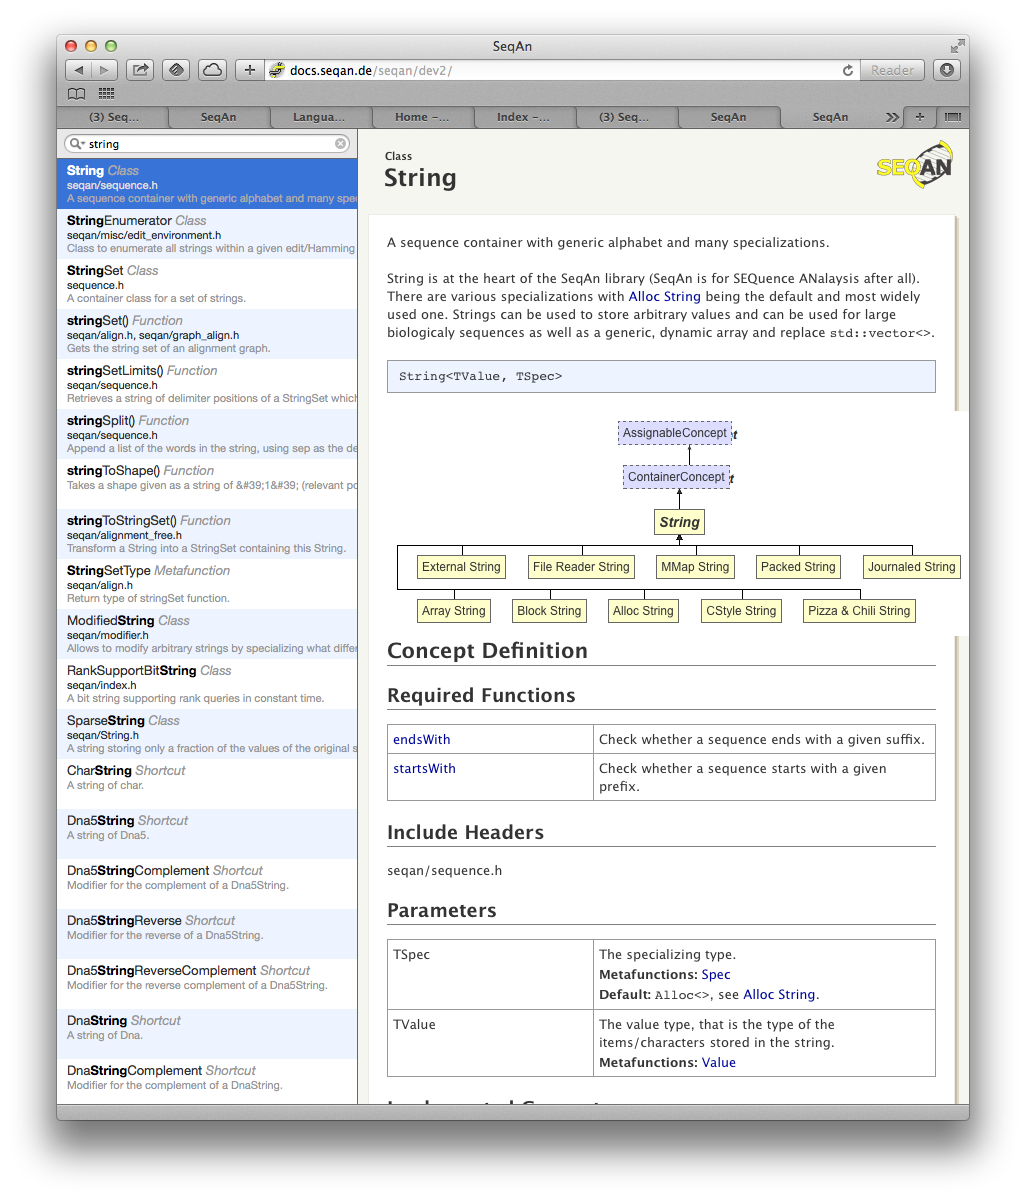
\includegraphics[width=\linewidth]{Figures/dox/dox-2_0_0-small-string-opened.png}
                \caption{Geöffnete \texttt{String}-Klasse in Version 2.0.0}
                \label{fig:dox-small-string-opened-2.0.0}
        \end{subfigure}
        \hfill
        \begin{subfigure}[b]{0.48\linewidth}
                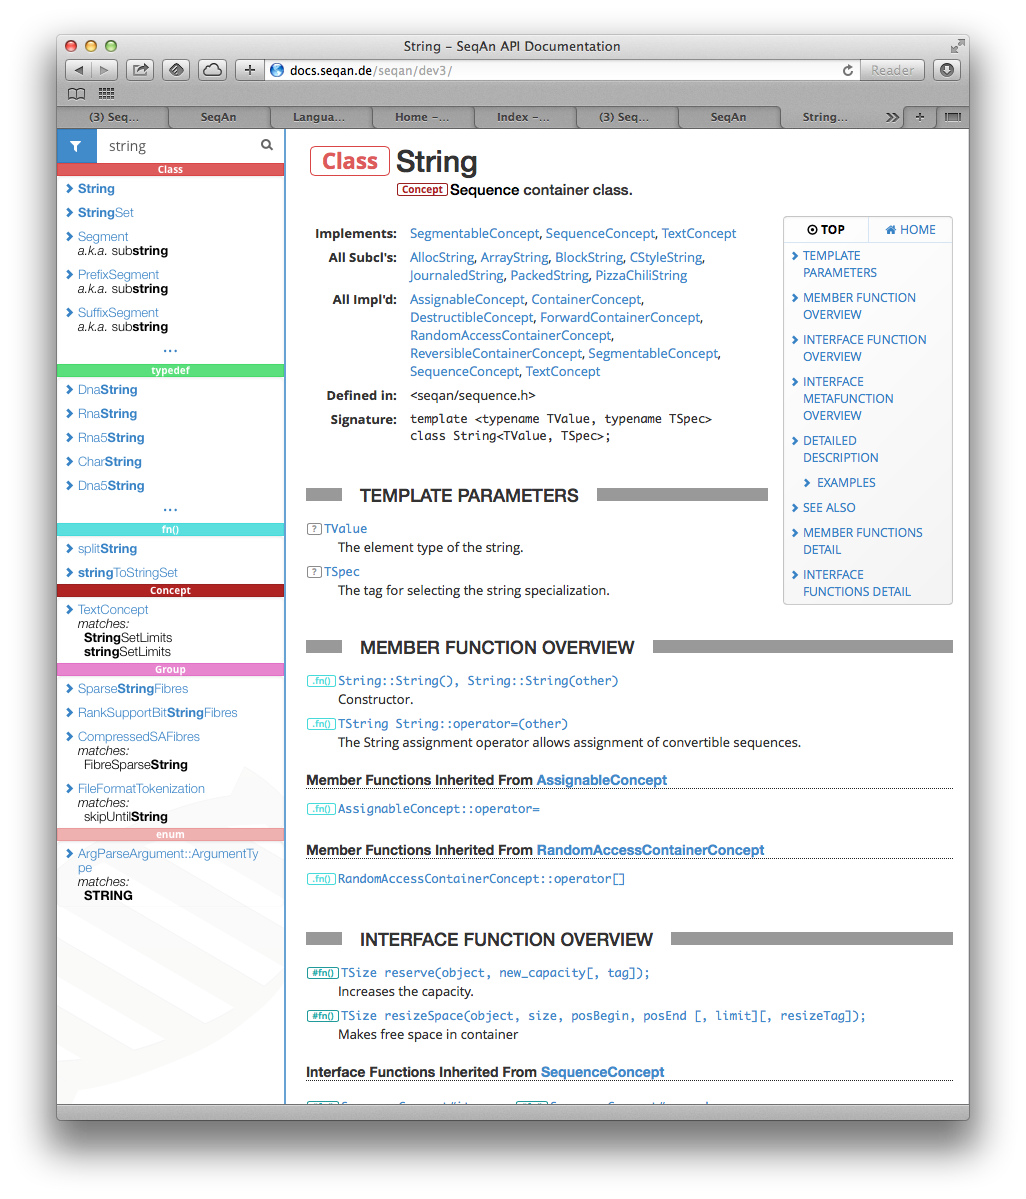
\includegraphics[width=\linewidth]{Figures/dox/dox-3_0_0-small-string-opened.png}
                \caption{Geöffnete \texttt{String}-Klasse in Version 3.0.0}
                \label{fig:dox-small-string-opened-3.0.0}
        \end{subfigure}
        \caption[Alte und neue Dokumentation im Vergleich --- in smaler Breite]{Die Abbildungen zeigen die alte und neue Dokumentation in schmaler Breite.}
        \label{fig:dox-small-all}
\end{figure}
%\end{landscape}
\restoregeometry




\paragraph{Integration}

Die neue Dokumentation ist besser in anderen Lernressourcen, wie den Tutorials, integriert. Dies wurde nicht zuletzt durch den weiter oben beschrieben Entwicklermodus gefördert, der SeqAn-Entwicklern alle möglichen Links für einen Dokumentations-(teil-)eintrag bereitstellt.  

Außerdem habe ich bei der Neuentwicklung auf die Indexierbarkeit durch Suchmaschinen geachtet. Dazu habe ich das Programm, welches die Dokumentation generiert, so angepasst, dass Inhalte sowohl statisch (für Suchmaschinen), als auch dynamisch (für Anwender) vorliegen.

Des Weiteren erfordert die Dokumentation --- trotz seines Funktionszuwachses --- keine Server-Komponente. Die mit SeqAn heruntergeladene Dokumentation verfügt online wie offline über den gleichen Funktionsumfang.







\begin{comment}
\newlength{\doxlargewidth}
\setlength{\doxlargewidth}{\linewidth}

\newlength{\doxnarrowwidth}
\setlength{\doxnarrowwidth}{0.61\doxlargewidth}

Donec urna leo, vulputate vitae porta eu, vehicula blandit libero. Phasellus eget massa et leo condimentum mollis. Nullam molestie, justo at pellentesque vulputate, sapien velit ornare diam, nec gravida lacus augue non diam. Integer mattis lacus id libero ultrices sit amet mollis neque molestie. Integer ut leo eget mi volutpat congue. Vivamus sodales, turpis id venenatis placerat, tellus purus adipiscing magna, eu aliquam nibh dolor id nibh. Pellentesque habitant morbi tristique senectus et netus et malesuada fames ac turpis egestas. Sed cursus convallis quam nec vehicula. Sed vulputate neque eget odio fringilla ac sodales urna feugiat.

\begin{figure}
  \centering
    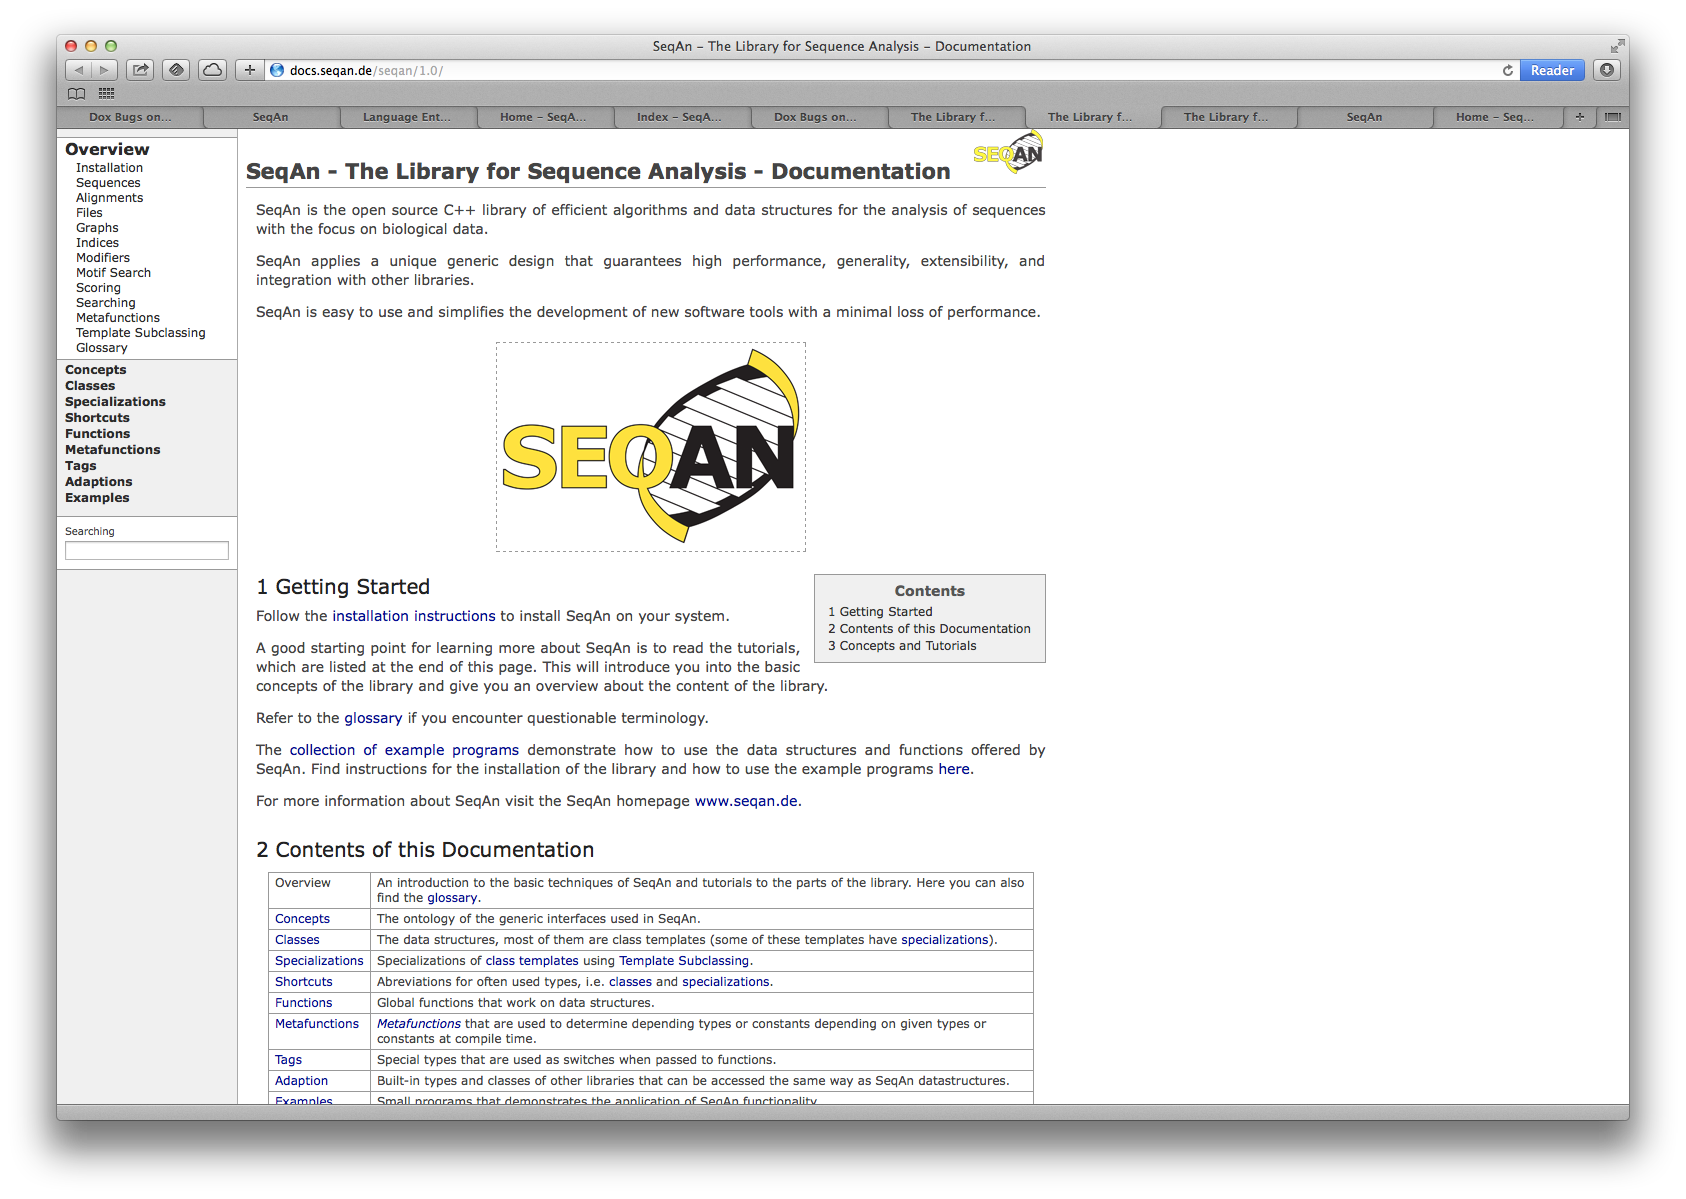
\includegraphics[width=\doxlargewidth]{Figures/dox/dox-1_0_0-large-home.png}
    \caption{Seqan-Online-Dokumentation in Version 1.0 - Breite Ansicht - Startseite}
    \label{fig:dox-1_0_0-large-home}
\end{figure}

\begin{figure}
  \centering
    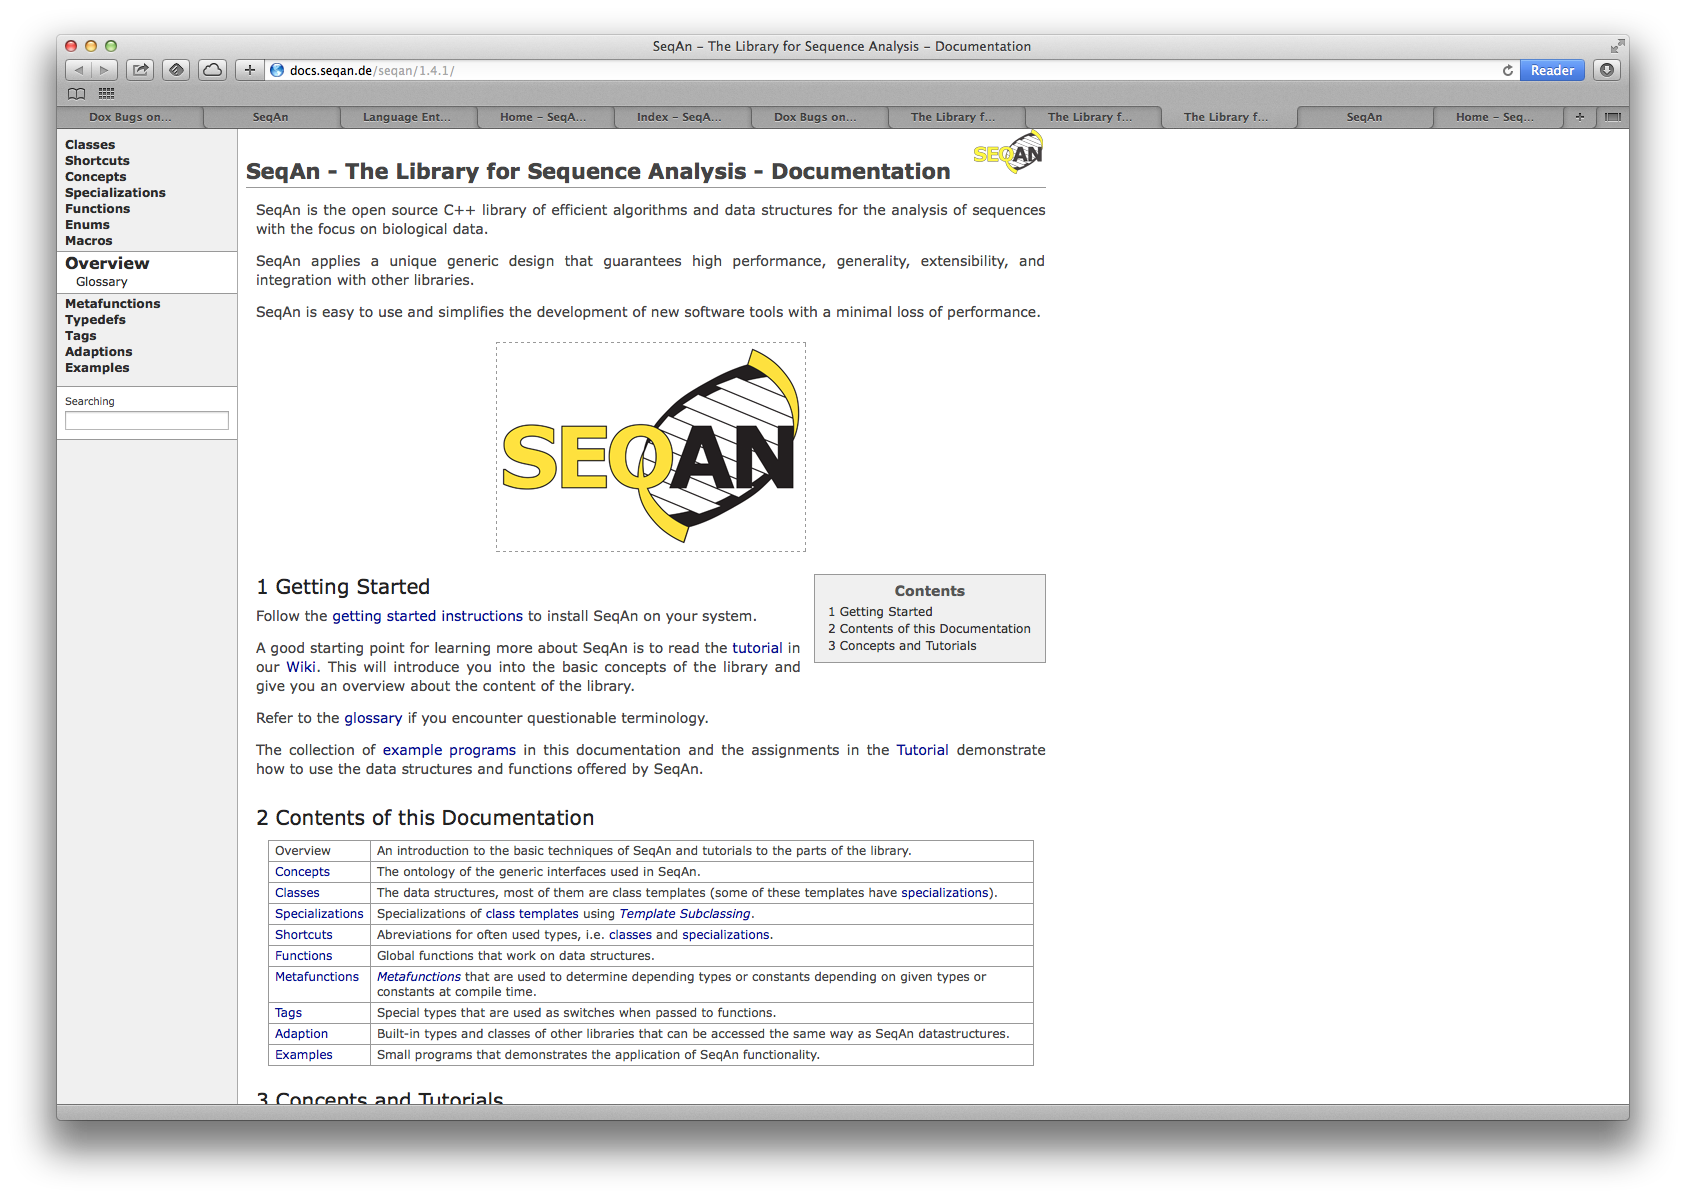
\includegraphics[width=\doxlargewidth]{Figures/dox/dox-1_4_1-large-home.png}
    \caption{Seqan-Online-Dokumentation in Version 1.4.1 - Breite Ansicht - Startseite}
    \label{fig:dox-1_4_1-large-home}
\end{figure}

Donec urna leo, vulputate vitae porta eu, vehicula blandit libero. Phasellus eget massa et leo condimentum mollis. Nullam molestie, justo at pellentesque vulputate, sapien velit ornare diam, nec gravida lacus augue non diam. Integer mattis lacus id libero ultrices sit amet mollis neque molestie. Integer ut leo eget mi volutpat congue. Vivamus sodales, turpis id venenatis placerat, tellus purus adipiscing magna, eu aliquam nibh dolor id nibh. Pellentesque habitant morbi tristique senectus et netus et malesuada fames ac turpis egestas. Sed cursus convallis quam nec vehicula. Sed vulputate neque eget odio fringilla ac sodales urna feugiat.

\begin{figure}
  \centering
    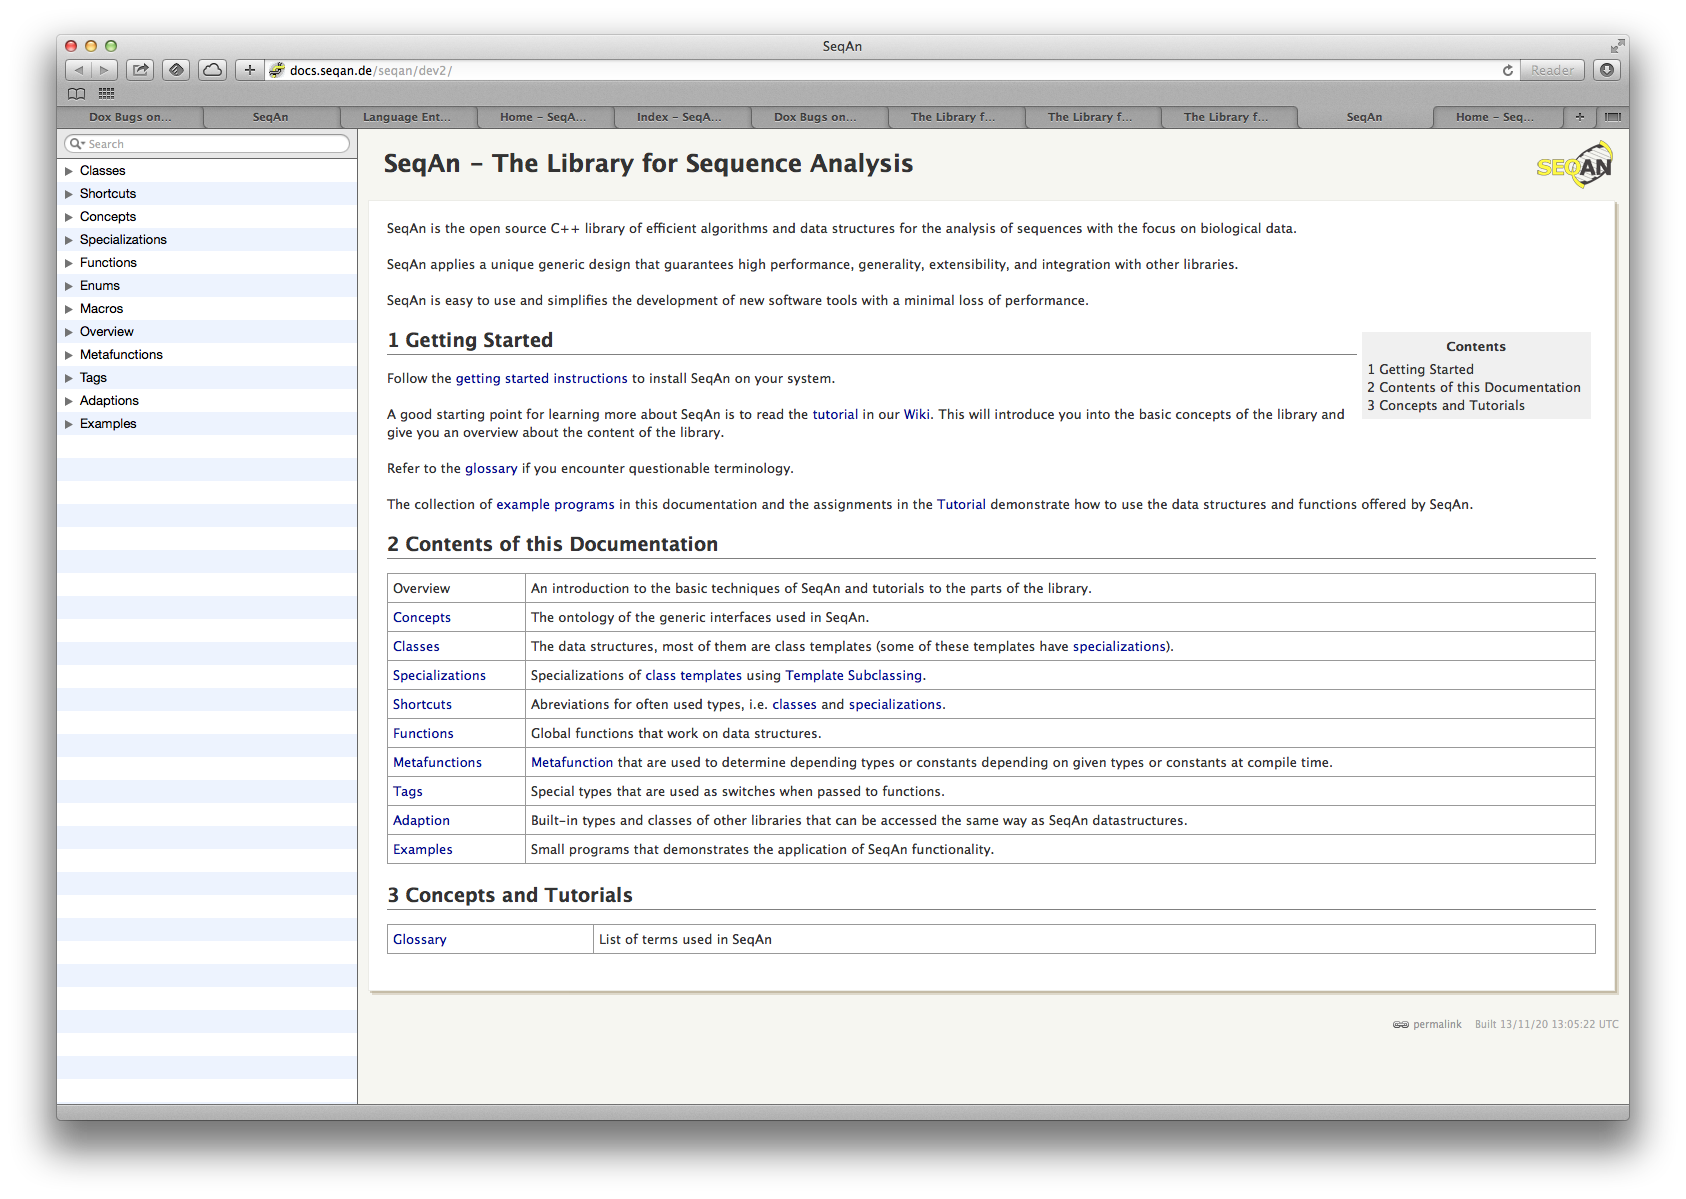
\includegraphics[width=\doxlargewidth]{Figures/dox/dox-2_0_0-large-home.png}
    \caption{Seqan-Online-Dokumentation in Version 2.0 - Breite Ansicht - Startseite}
    \label{fig:dox-2_0_0-large-home}
\end{figure}

\begin{figure}
  \centering
    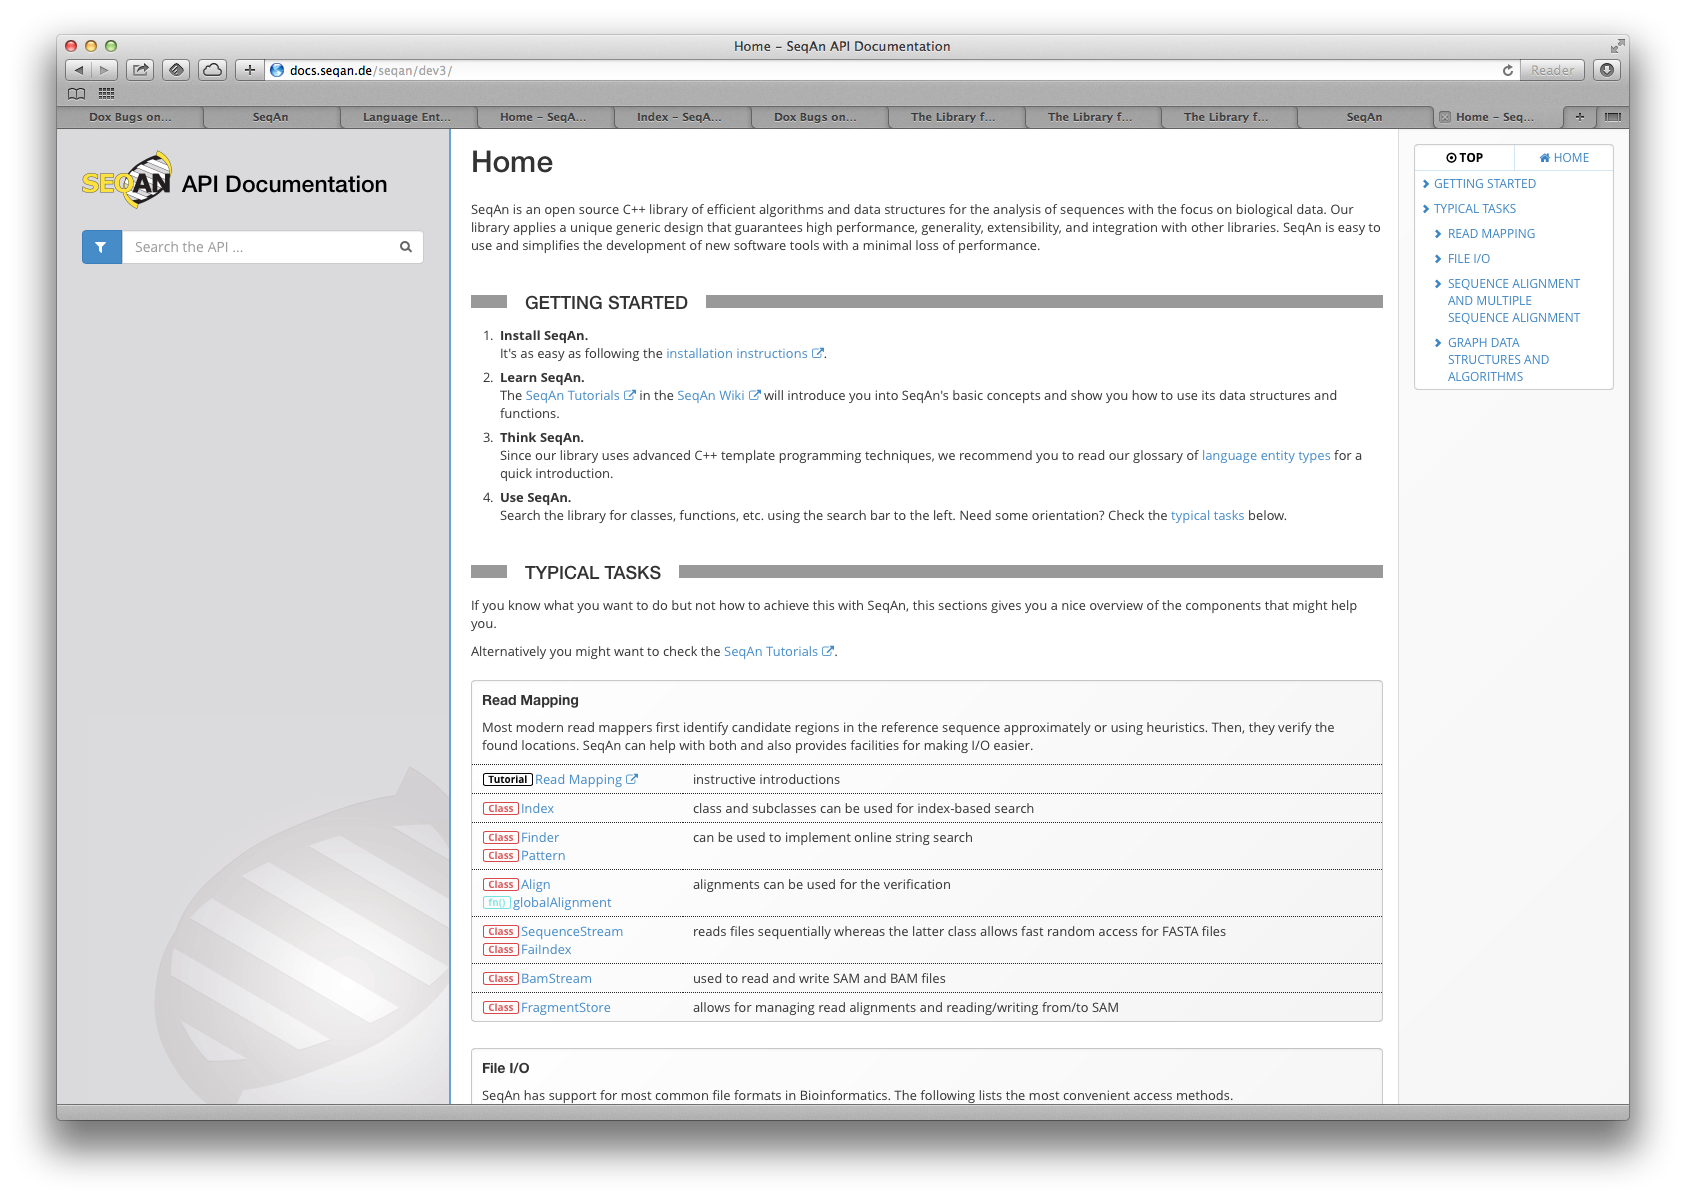
\includegraphics[width=\doxlargewidth]{Figures/dox/dox-3_0_0-large-home.png}
    \caption{Seqan-Online-Dokumentation in Version 3.0 - Breite Ansicht - Startseite}
    \label{fig:dox-3_0_0-large-home}
\end{figure}

Donec urna leo, vulputate vitae porta eu, vehicula blandit libero. Phasellus eget massa et leo condimentum mollis. Nullam molestie, justo at pellentesque vulputate, sapien velit ornare diam, nec gravida lacus augue non diam. Integer mattis lacus id libero ultrices sit amet mollis neque molestie. Integer ut leo eget mi volutpat congue. Vivamus sodales, turpis id venenatis placerat, tellus purus adipiscing magna, eu aliquam nibh dolor id nibh. Pellentesque habitant morbi tristique senectus et netus et malesuada fames ac turpis egestas. Sed cursus convallis quam nec vehicula. Sed vulputate neque eget odio fringilla ac sodales urna feugiat.

Donec urna leo, vulputate vitae porta eu, vehicula blandit libero. Phasellus eget massa et leo condimentum mollis. Nullam molestie, justo at pellentesque vulputate, sapien velit ornare diam, nec gravida lacus augue non diam. Integer mattis lacus id libero ultrices sit amet mollis neque molestie. Integer ut leo eget mi volutpat congue. Vivamus sodales, turpis id venenatis placerat, tellus purus adipiscing magna, eu aliquam nibh dolor id nibh. Pellentesque habitant morbi tristique senectus et netus et malesuada fames ac turpis egestas. Sed cursus convallis quam nec vehicula. Sed vulputate neque eget odio fringilla ac sodales urna feugiat.


\begin{figure}
  \centering
    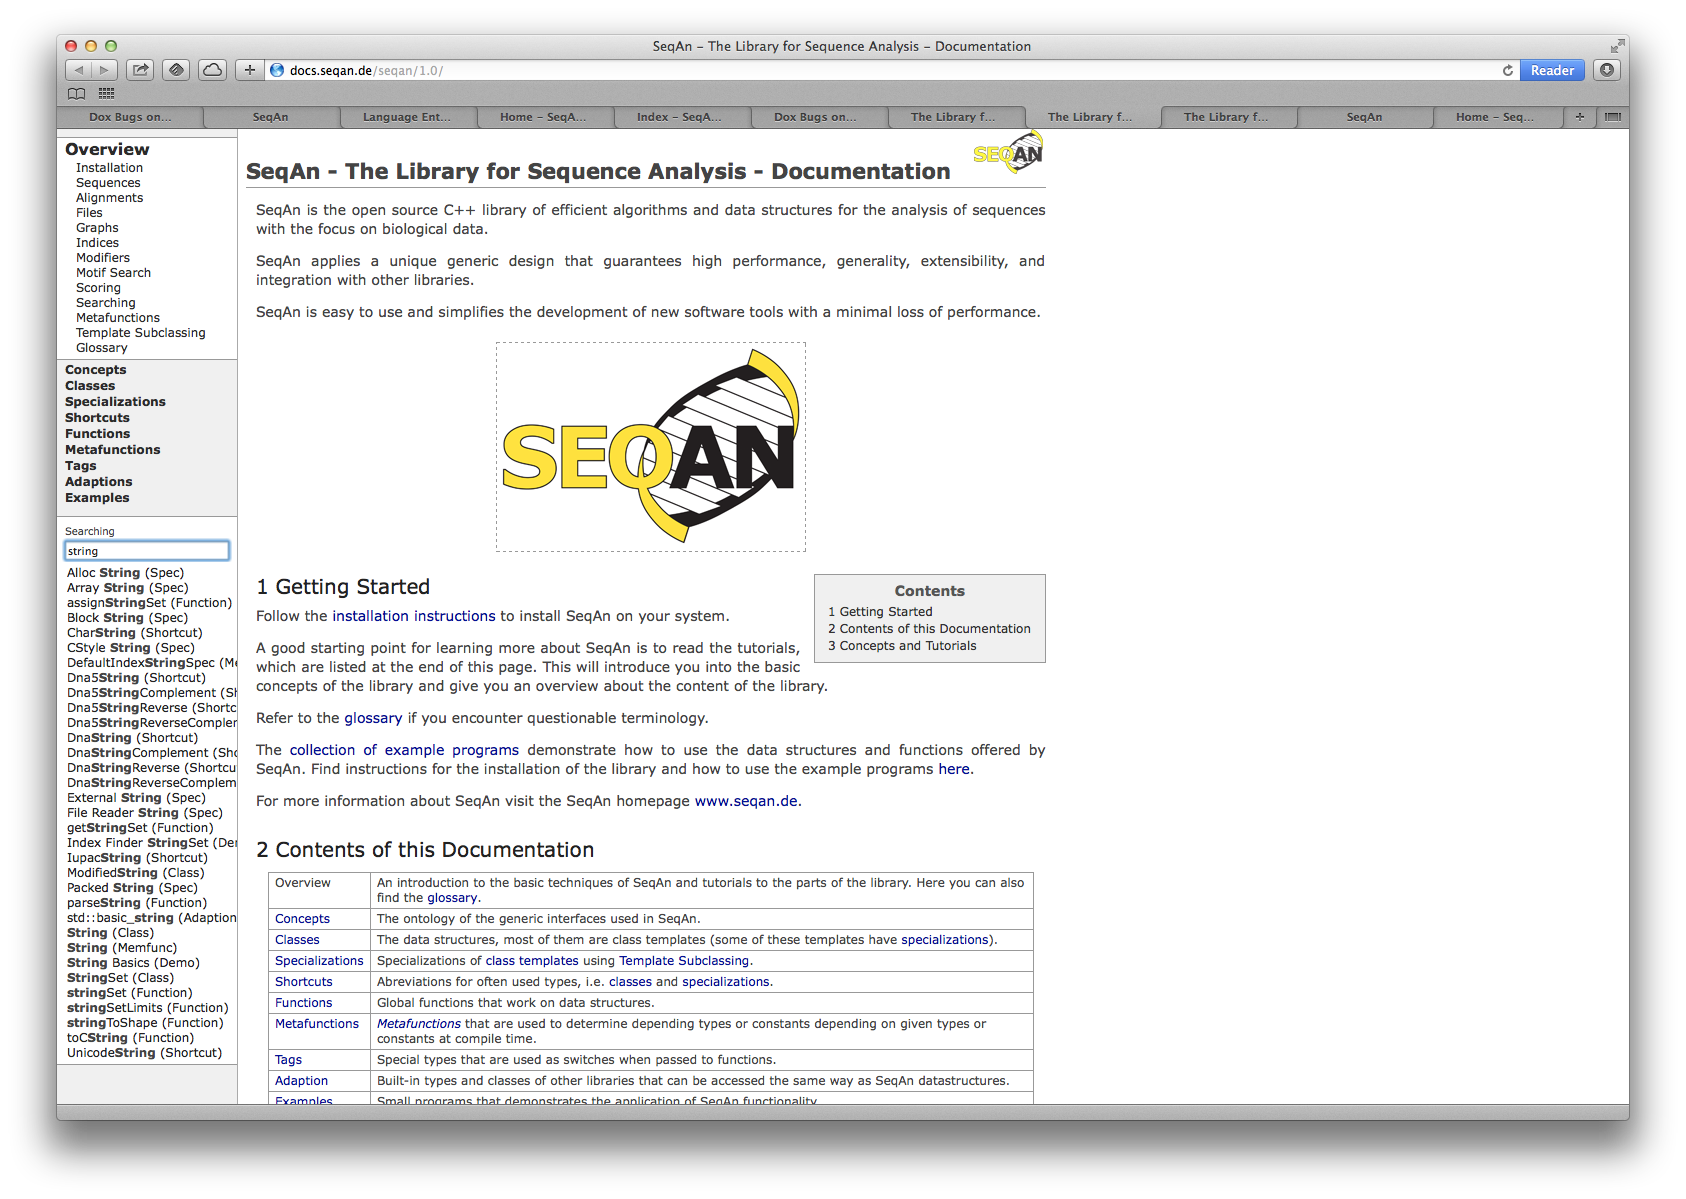
\includegraphics[width=\doxlargewidth]{Figures/dox/dox-1_0_0-large-string.png}
    \caption{Seqan-Online-Dokumentation in Version 1.0 - Breite Ansicht - Suche nach ``String''}
    \label{fig:dox-1_0_0-large-string}
\end{figure}

\begin{figure}
  \centering
    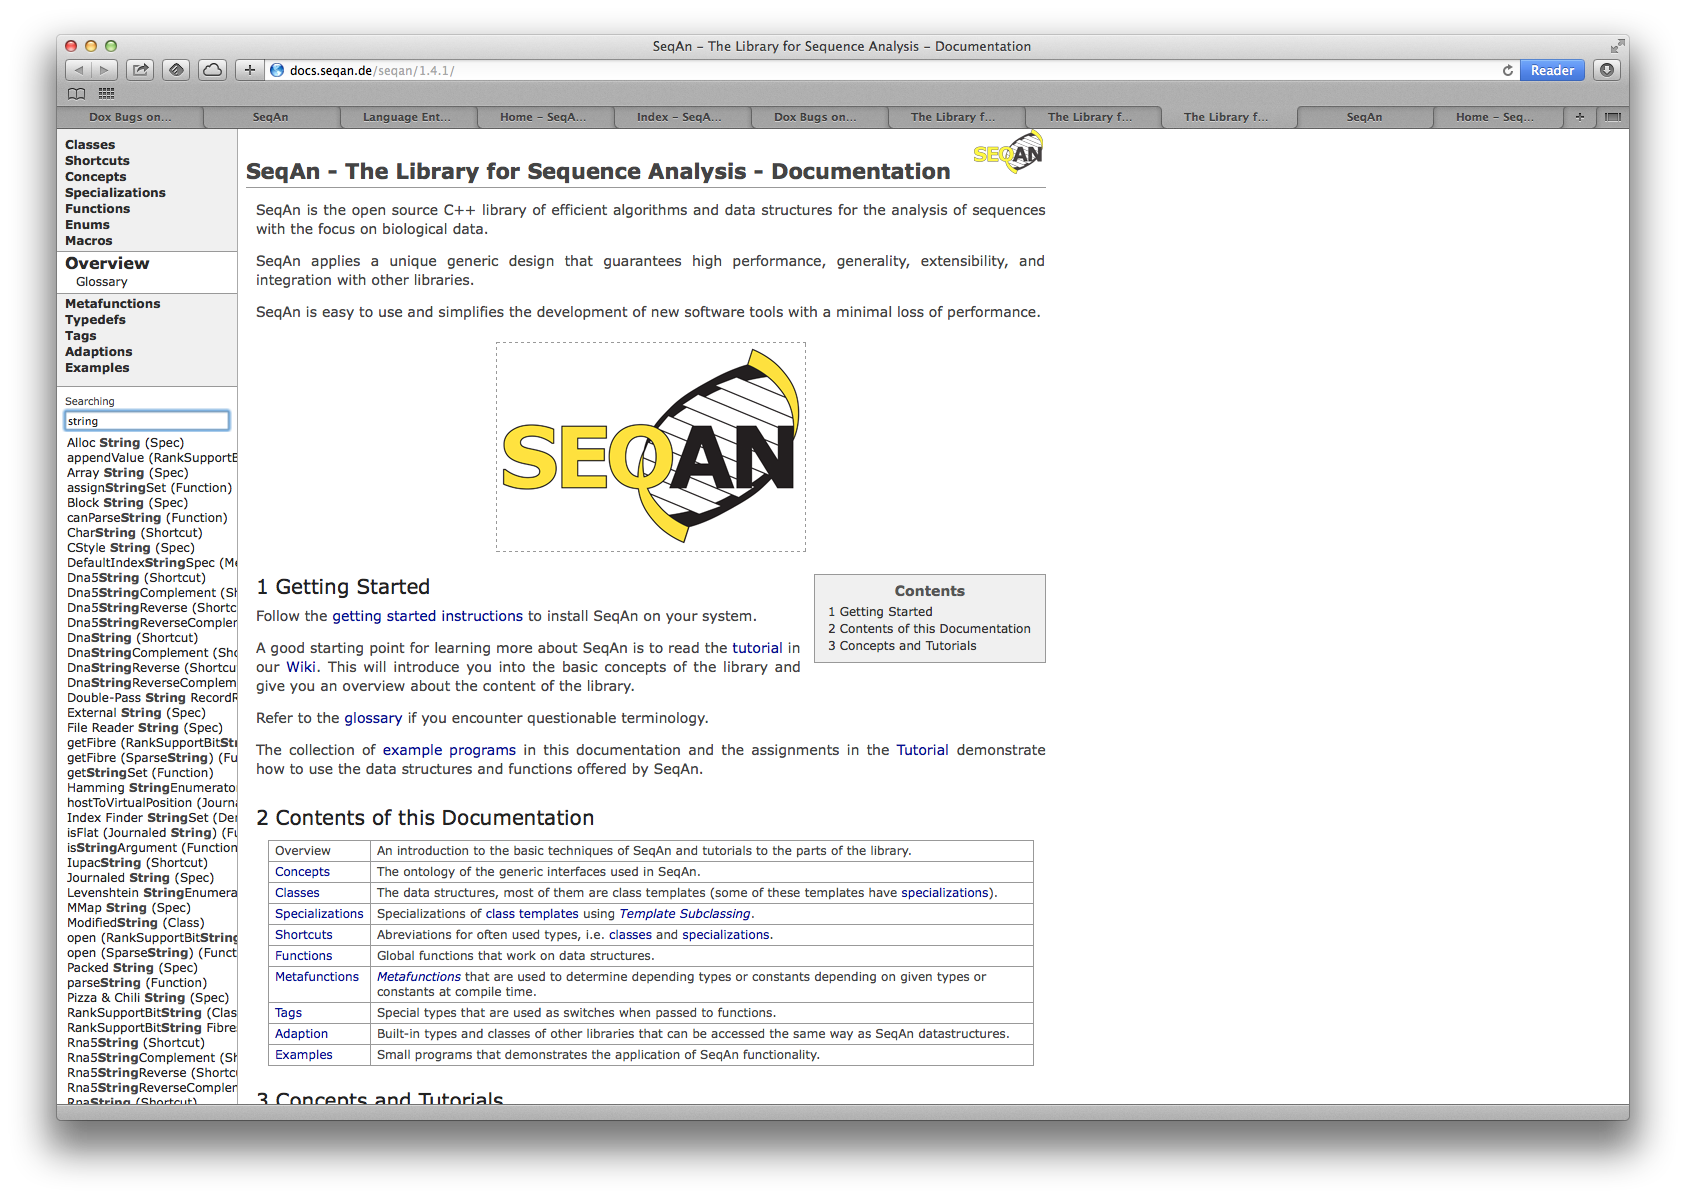
\includegraphics[width=\doxlargewidth]{Figures/dox/dox-1_4_1-large-string.png}
    \caption{Seqan-Online-Dokumentation in Version 1.4.1 - Breite Ansicht - Suche nach ``String''}
    \label{fig:dox-1_4_1-large-string}
\end{figure}

Donec urna leo, vulputate vitae porta eu, vehicula blandit libero. Phasellus eget massa et leo condimentum mollis. Nullam molestie, justo at pellentesque vulputate, sapien velit ornare diam, nec gravida lacus augue non diam. Integer mattis lacus id libero ultrices sit amet mollis neque molestie. Integer ut leo eget mi volutpat congue. Vivamus sodales, turpis id venenatis placerat, tellus purus adipiscing magna, eu aliquam nibh dolor id nibh. Pellentesque habitant morbi tristique senectus et netus et malesuada fames ac turpis egestas. Sed cursus convallis quam nec vehicula. Sed vulputate neque eget odio fringilla ac sodales urna feugiat.

\begin{figure}
  \centering
    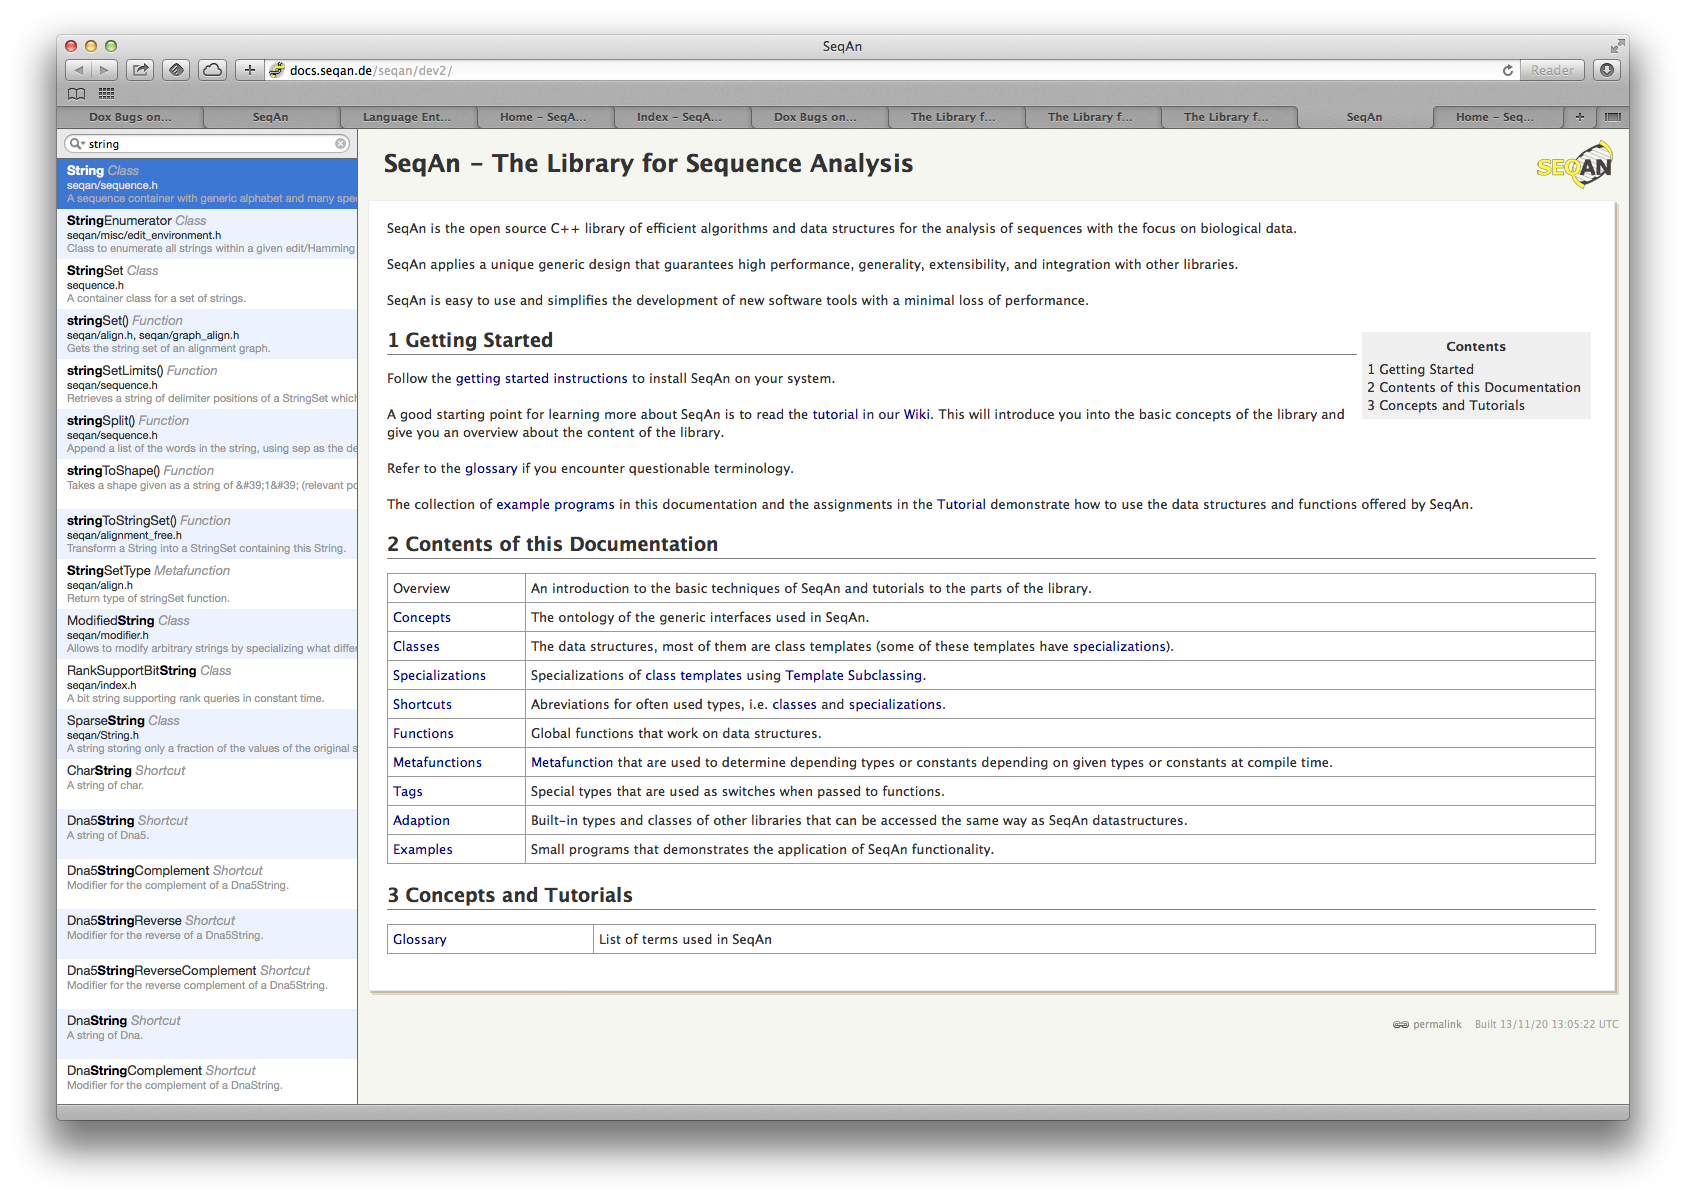
\includegraphics[width=\doxlargewidth]{Figures/dox/dox-2_0_0-large-string.png}
    \caption{Seqan-Online-Dokumentation in Version 2.0 - Breite Ansicht - Suche nach ``String''}
    \label{fig:dox-2_0_0-large-string}
\end{figure}

\begin{figure}
  \centering
    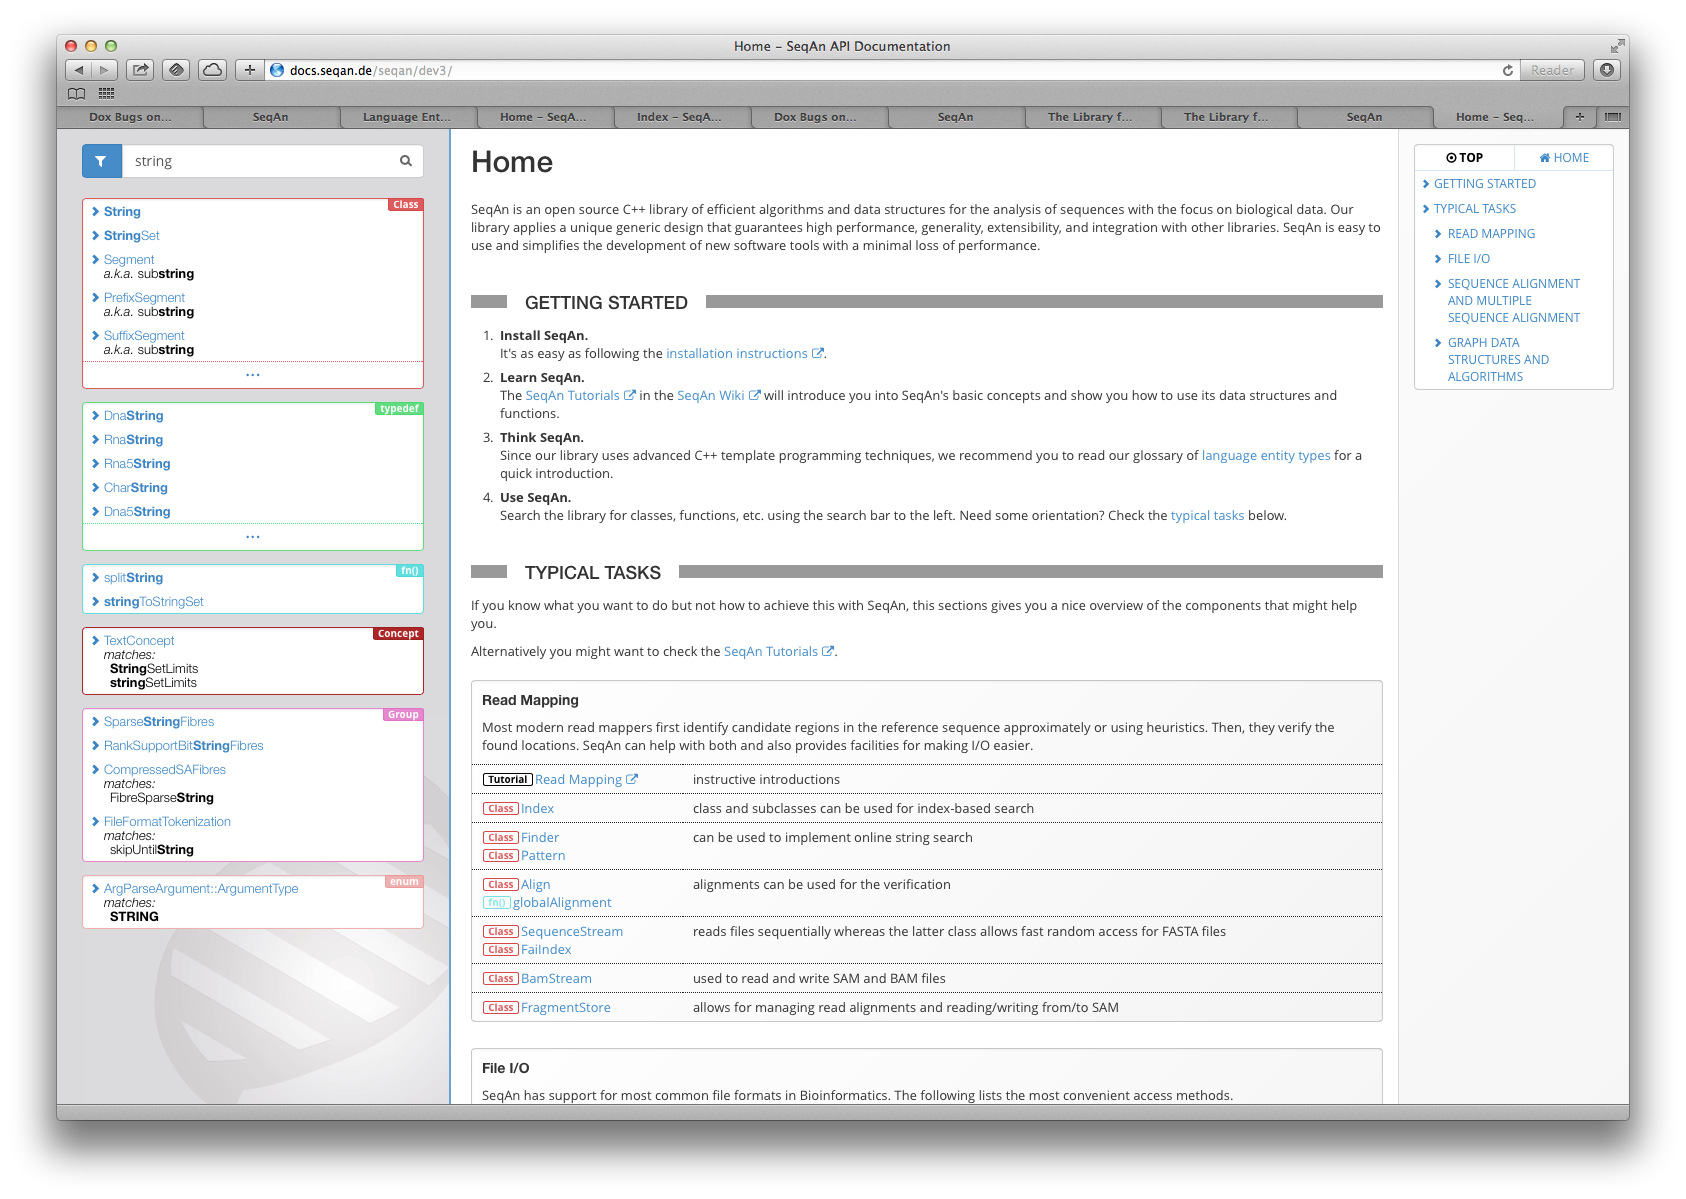
\includegraphics[width=\doxlargewidth]{Figures/dox/dox-3_0_0-large-string.png}
    \caption{Seqan-Online-Dokumentation in Version 3.0 - Breite Ansicht - Suche nach ``String''}
    \label{fig:dox-3_0_0-large-string}
\end{figure}

Donec urna leo, vulputate vitae porta eu, vehicula blandit libero. Phasellus eget massa et leo condimentum mollis. Nullam molestie, justo at pellentesque vulputate, sapien velit ornare diam, nec gravida lacus augue non diam. Integer mattis lacus id libero ultrices sit amet mollis neque molestie. Integer ut leo eget mi volutpat congue. Vivamus sodales, turpis id venenatis placerat, tellus purus adipiscing magna, eu aliquam nibh dolor id nibh. Pellentesque habitant morbi tristique senectus et netus et malesuada fames ac turpis egestas. Sed cursus convallis quam nec vehicula. Sed vulputate neque eget odio fringilla ac sodales urna feugiat.

\begin{figure}
  \centering
    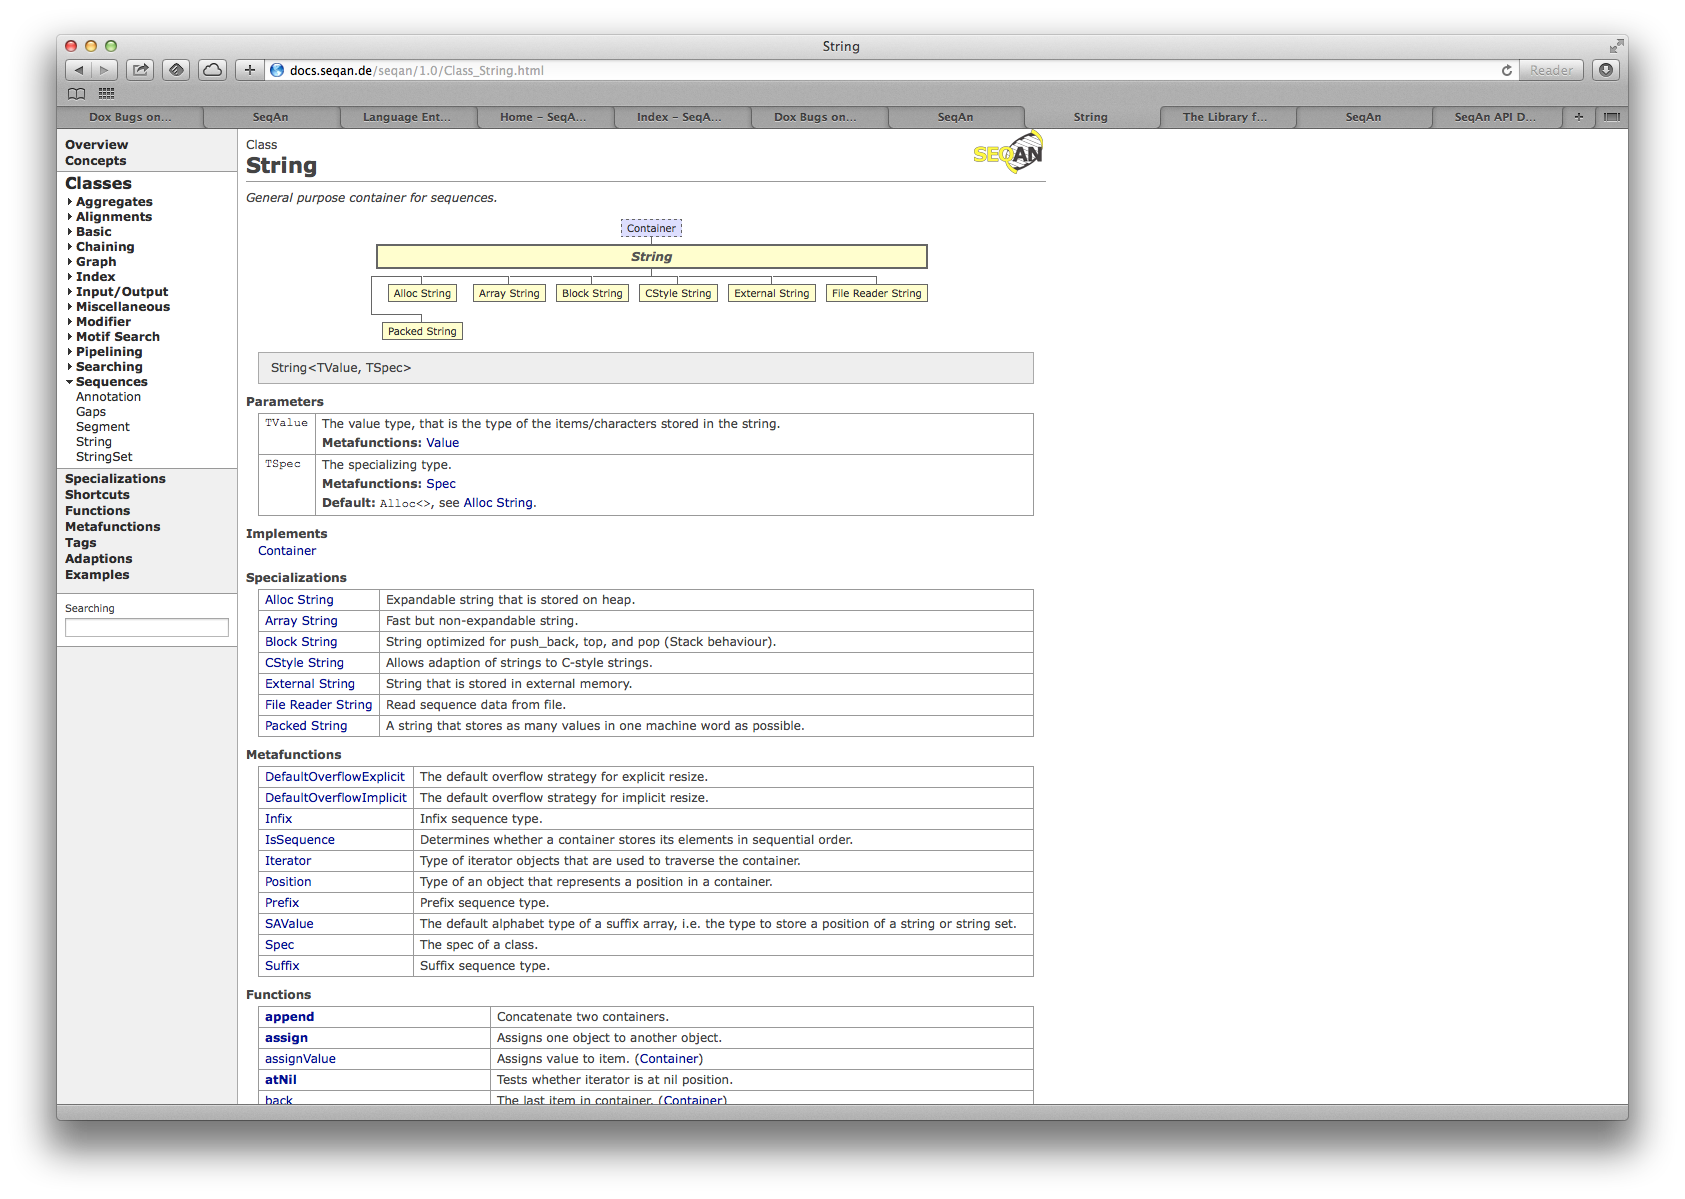
\includegraphics[width=\doxlargewidth]{Figures/dox/dox-1_0_0-large-string-opened.png}
    \caption{Seqan-Online-Dokumentation in Version 1.0 - Breite Ansicht - Klasse ``String''}
    \label{fig:dox-1_0_0-large-string-opened}
\end{figure}

\begin{figure}
  \centering
    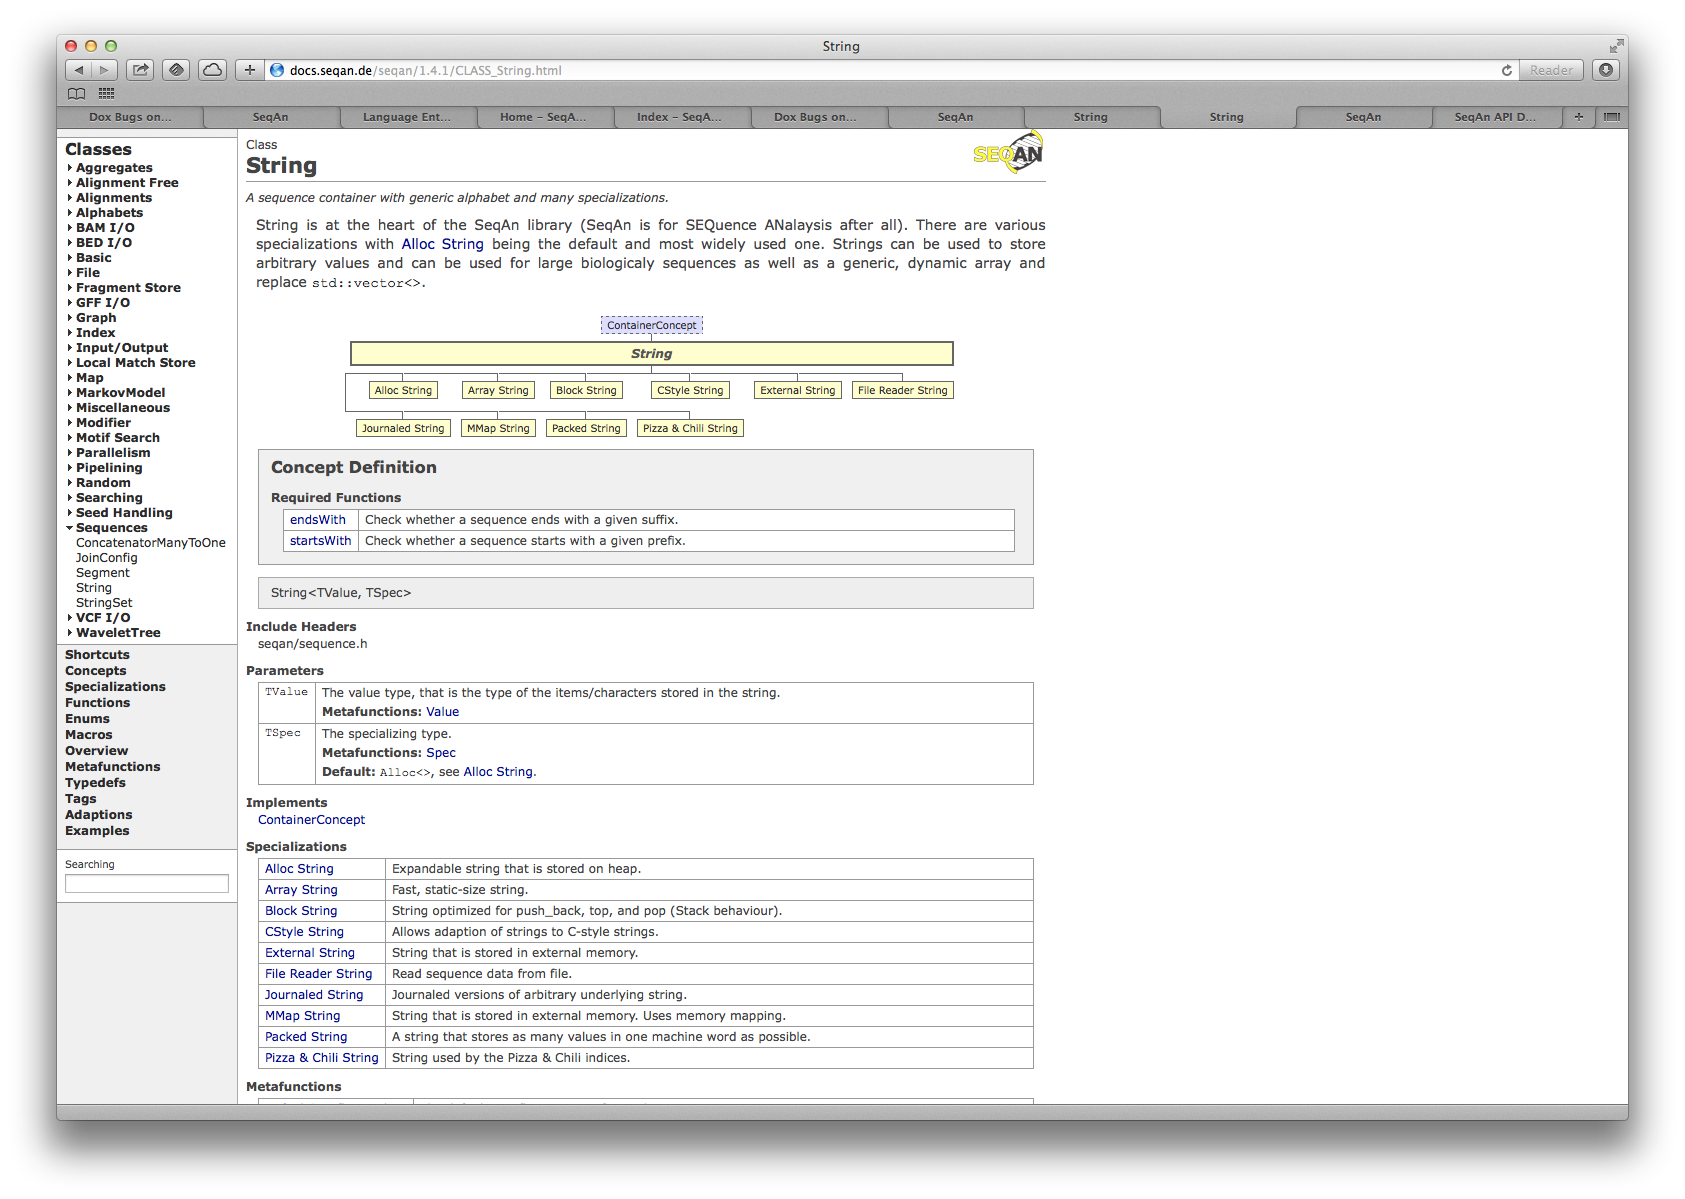
\includegraphics[width=\doxlargewidth]{Figures/dox/dox-1_4_1-large-string-opened.png}
    \caption{Seqan-Online-Dokumentation in Version 1.4.1 - Breite Ansicht - Klasse ``String''}
    \label{fig:dox-1_4_1-large-string-opened}
\end{figure}

Donec urna leo, vulputate vitae porta eu, vehicula blandit libero. Phasellus eget massa et leo condimentum mollis. Nullam molestie, justo at pellentesque vulputate, sapien velit ornare diam, nec gravida lacus augue non diam. Integer mattis lacus id libero ultrices sit amet mollis neque molestie. Integer ut leo eget mi volutpat congue. Vivamus sodales, turpis id venenatis placerat, tellus purus adipiscing magna, eu aliquam nibh dolor id nibh. Pellentesque habitant morbi tristique senectus et netus et malesuada fames ac turpis egestas. Sed cursus convallis quam nec vehicula. Sed vulputate neque eget odio fringilla ac sodales urna feugiat.

Donec urna leo, vulputate vitae porta eu, vehicula blandit libero. Phasellus eget massa et leo condimentum mollis. Nullam molestie, justo at pellentesque vulputate, sapien velit ornare diam, nec gravida lacus augue non diam. Integer mattis lacus id libero ultrices sit amet mollis neque molestie. Integer ut leo eget mi volutpat congue. Vivamus sodales, turpis id venenatis placerat, tellus purus adipiscing magna, eu aliquam nibh dolor id nibh. Pellentesque habitant morbi tristique senectus et netus et malesuada fames ac turpis egestas. Sed cursus convallis quam nec vehicula. Sed vulputate neque eget odio fringilla ac sodales urna feugiat.

\begin{figure}
  \centering
    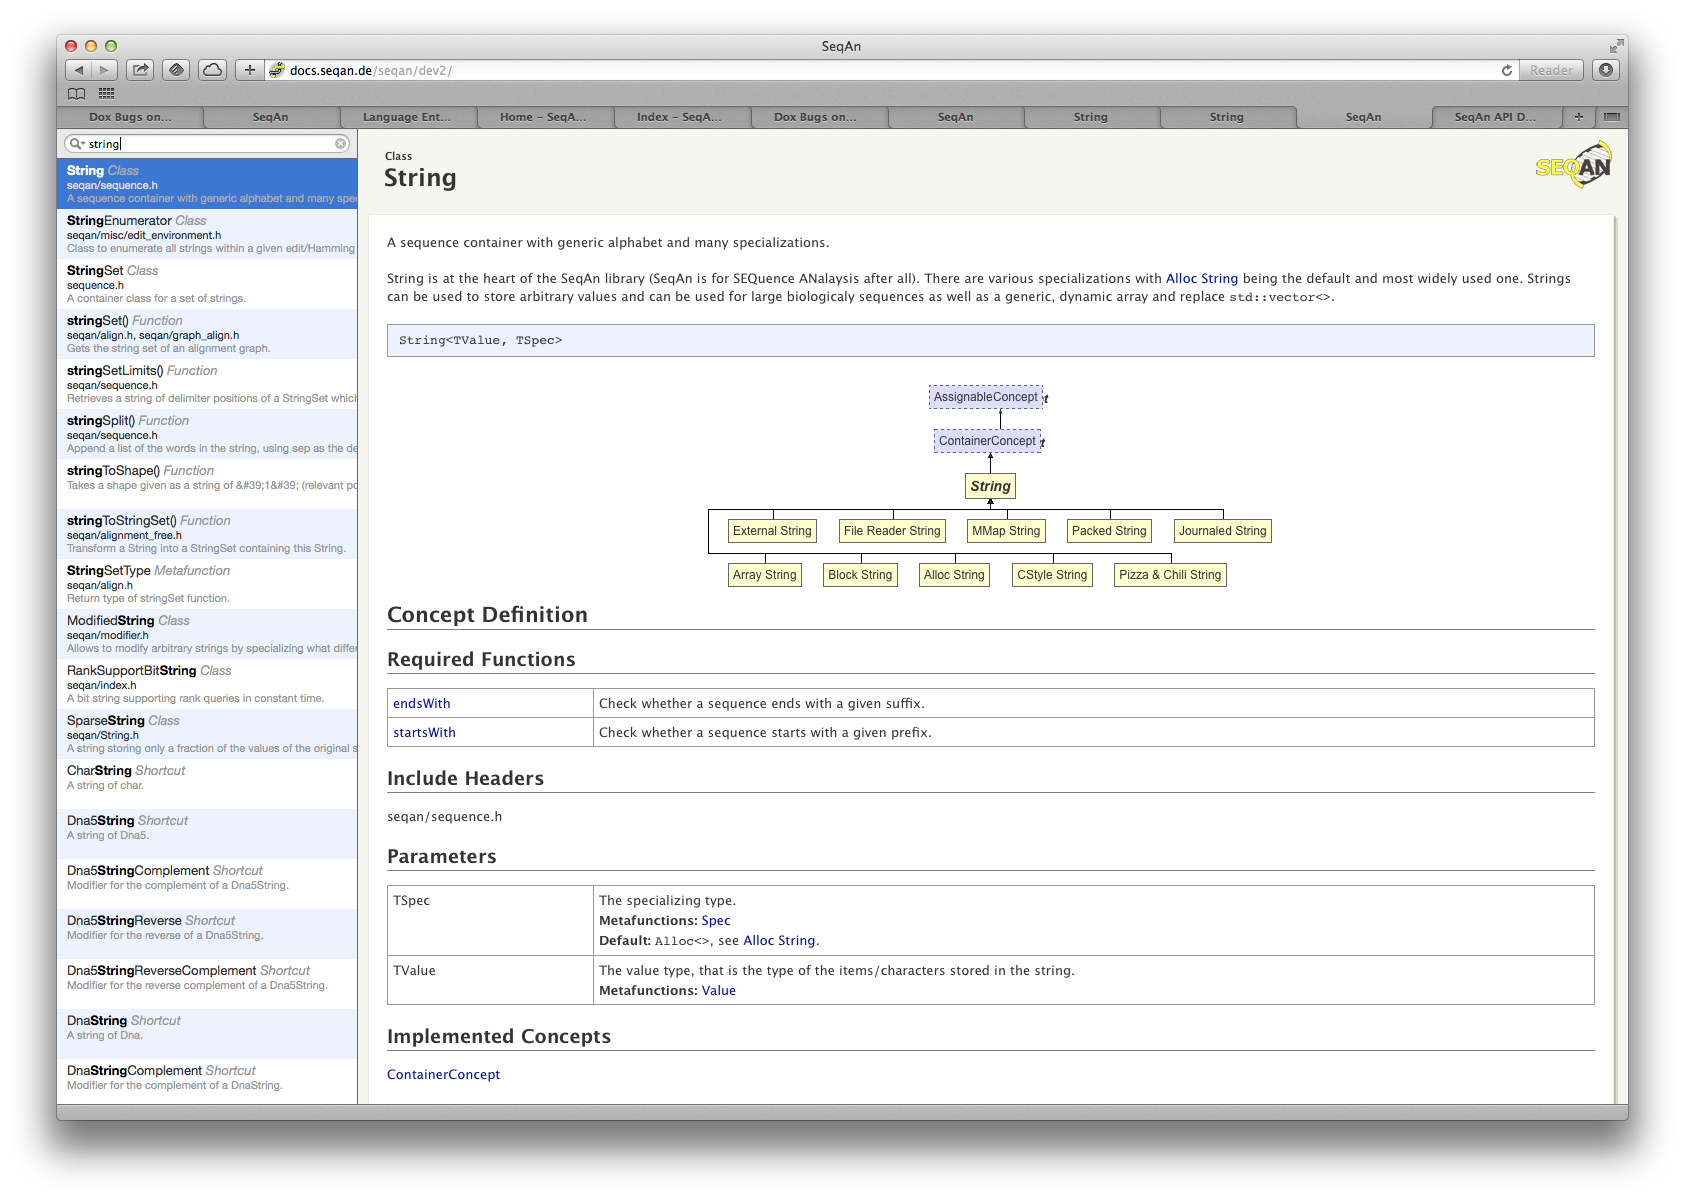
\includegraphics[width=\doxlargewidth]{Figures/dox/dox-2_0_0-large-string-opened.png}
    \caption{Seqan-Online-Dokumentation in Version 2.0 - Breite Ansicht - Klasse ``String''}
    \label{fig:dox-2_0_0-large-string-opened}
\end{figure}

\begin{figure}
  \centering
    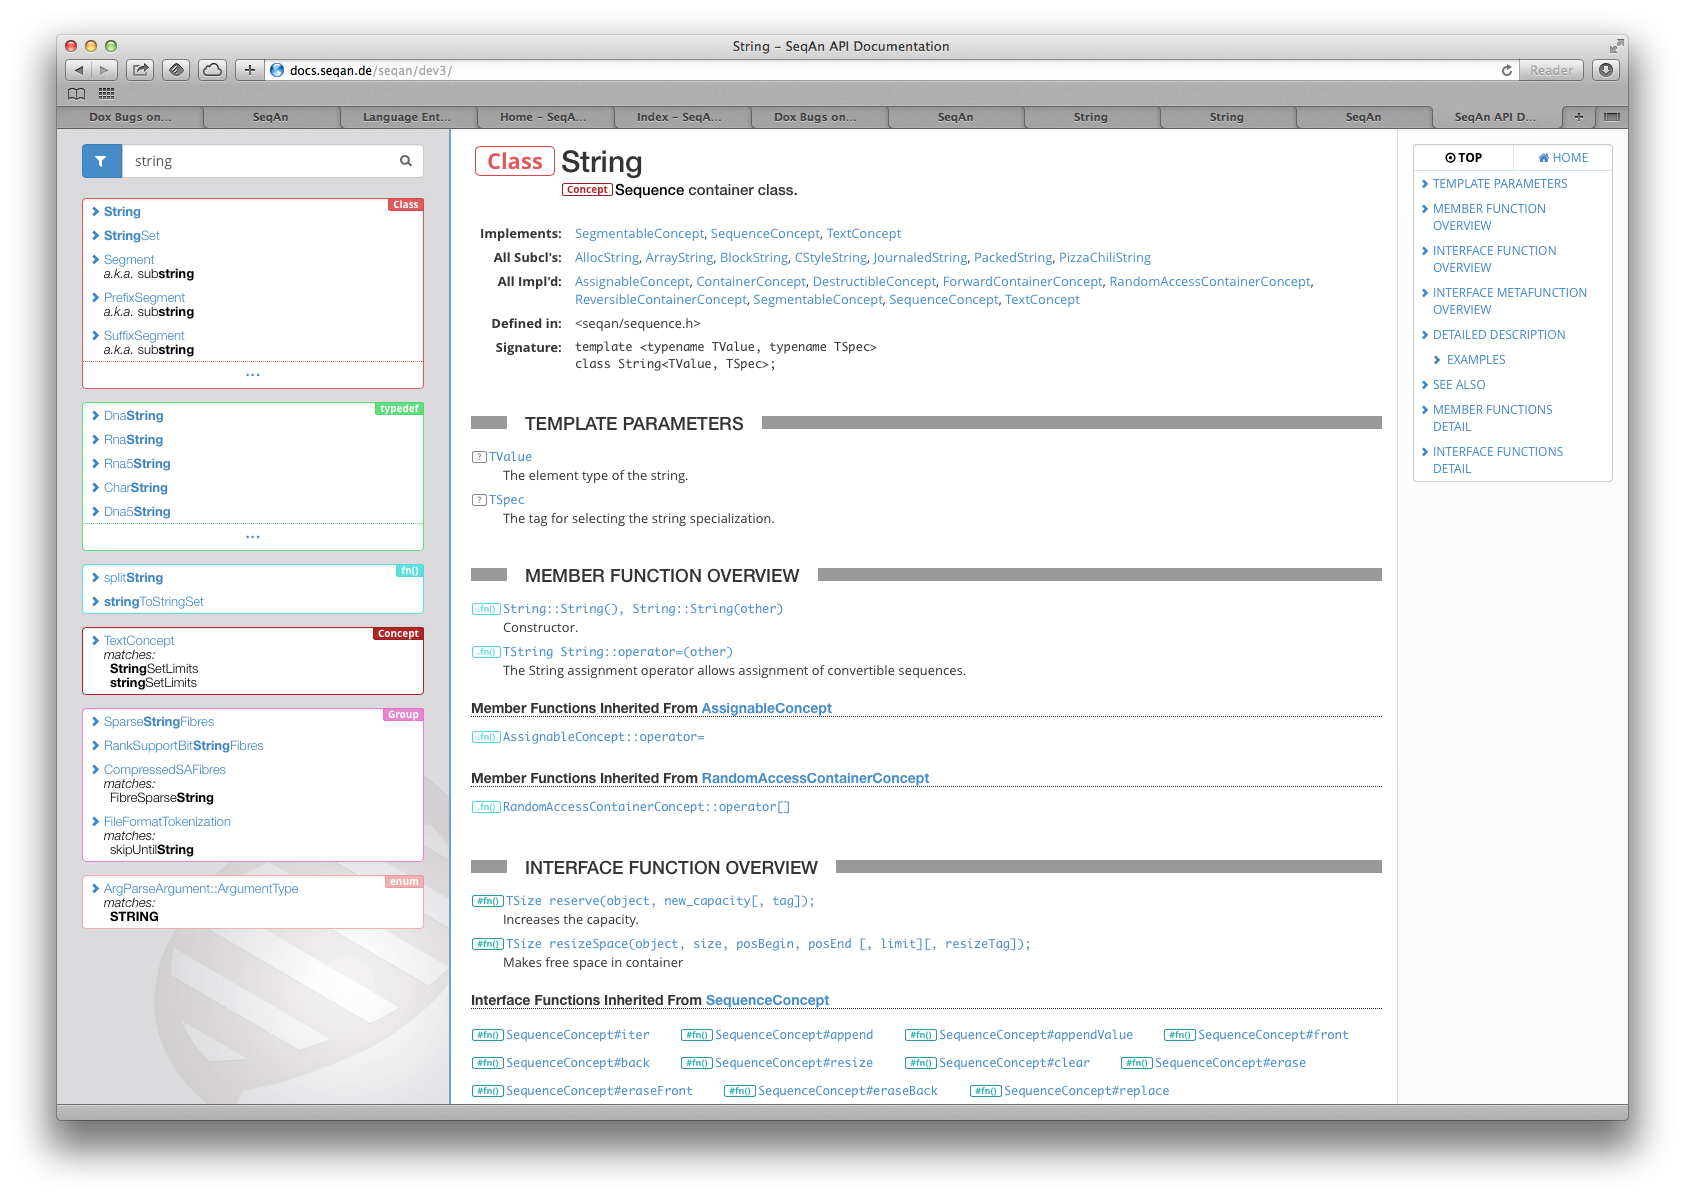
\includegraphics[width=\doxlargewidth]{Figures/dox/dox-3_0_0-large-string-opened.png}
    \caption{Seqan-Online-Dokumentation in Version 3.0 - Breite Ansicht - Klasse ``String''}
    \label{fig:dox-3_0_0-large-string-opened}
\end{figure}

Donec urna leo, vulputate vitae porta eu, vehicula blandit libero. Phasellus eget massa et leo condimentum mollis. Nullam molestie, justo at pellentesque vulputate, sapien velit ornare diam, nec gravida lacus augue non diam. Integer mattis lacus id libero ultrices sit amet mollis neque molestie. Integer ut leo eget mi volutpat congue. Vivamus sodales, turpis id venenatis placerat, tellus purus adipiscing magna, eu aliquam nibh dolor id nibh. Pellentesque habitant morbi tristique senectus et netus et malesuada fames ac turpis egestas. Sed cursus convallis quam nec vehicula. Sed vulputate neque eget odio fringilla ac sodales urna feugiat.

Donec urna leo, vulputate vitae porta eu, vehicula blandit libero. Phasellus eget massa et leo condimentum mollis. Nullam molestie, justo at pellentesque vulputate, sapien velit ornare diam, nec gravida lacus augue non diam. Integer mattis lacus id libero ultrices sit amet mollis neque molestie. Integer ut leo eget mi volutpat congue. Vivamus sodales, turpis id venenatis placerat, tellus purus adipiscing magna, eu aliquam nibh dolor id nibh. Pellentesque habitant morbi tristique senectus et netus et malesuada fames ac turpis egestas. Sed cursus convallis quam nec vehicula. Sed vulputate neque eget odio fringilla ac sodales urna feugiat.

\begin{figure}
  \centering
    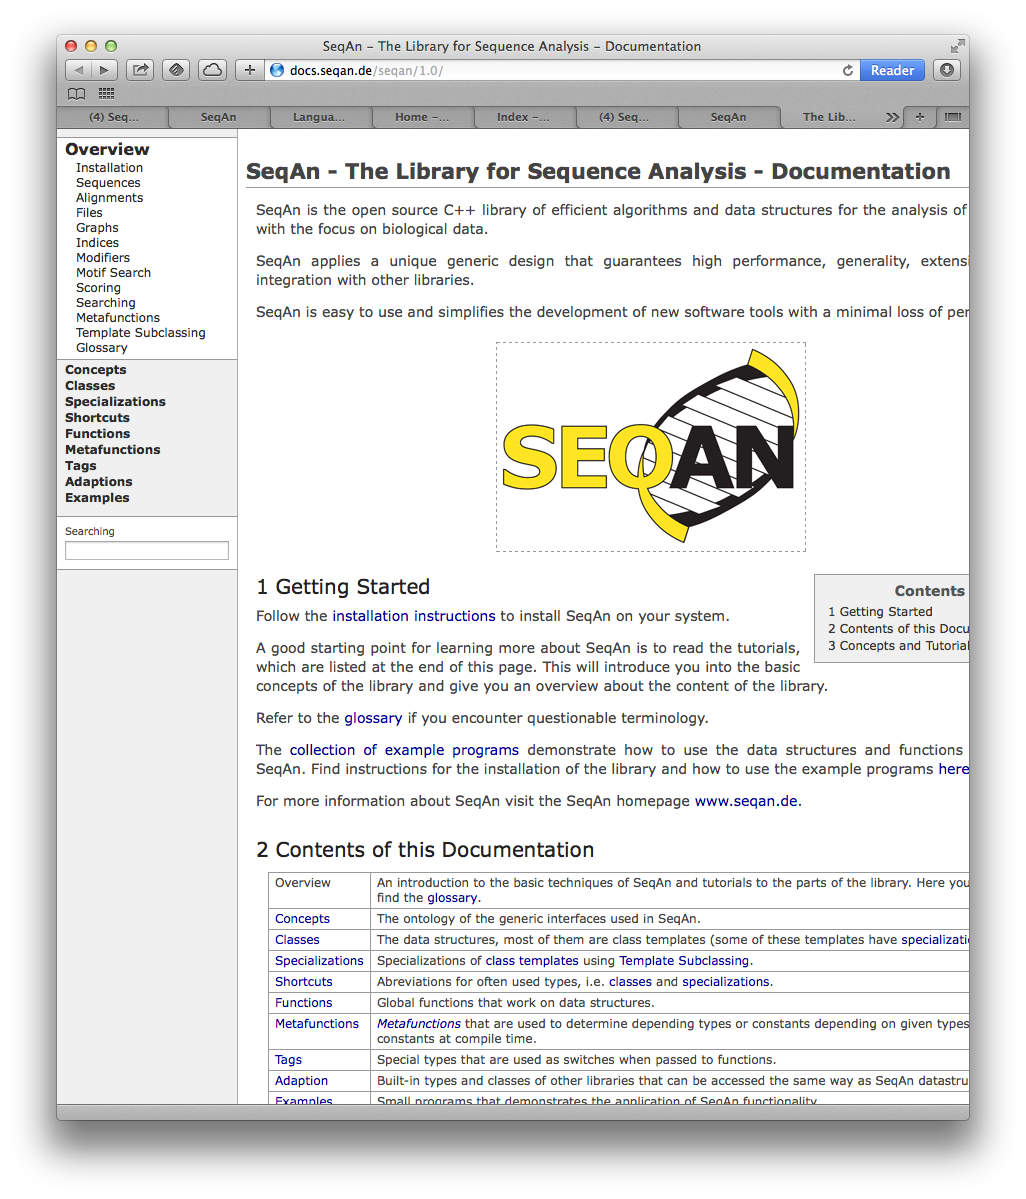
\includegraphics[width=\doxnarrowwidth]{Figures/dox/dox-1_0_0-small-home.png}
    \caption{Seqan-Online-Dokumentation in Version 1.0 - Smale Ansicht - Startseite}
    \label{fig:dox-1_0_0-small-home}
\end{figure}

\begin{figure}
  \centering
    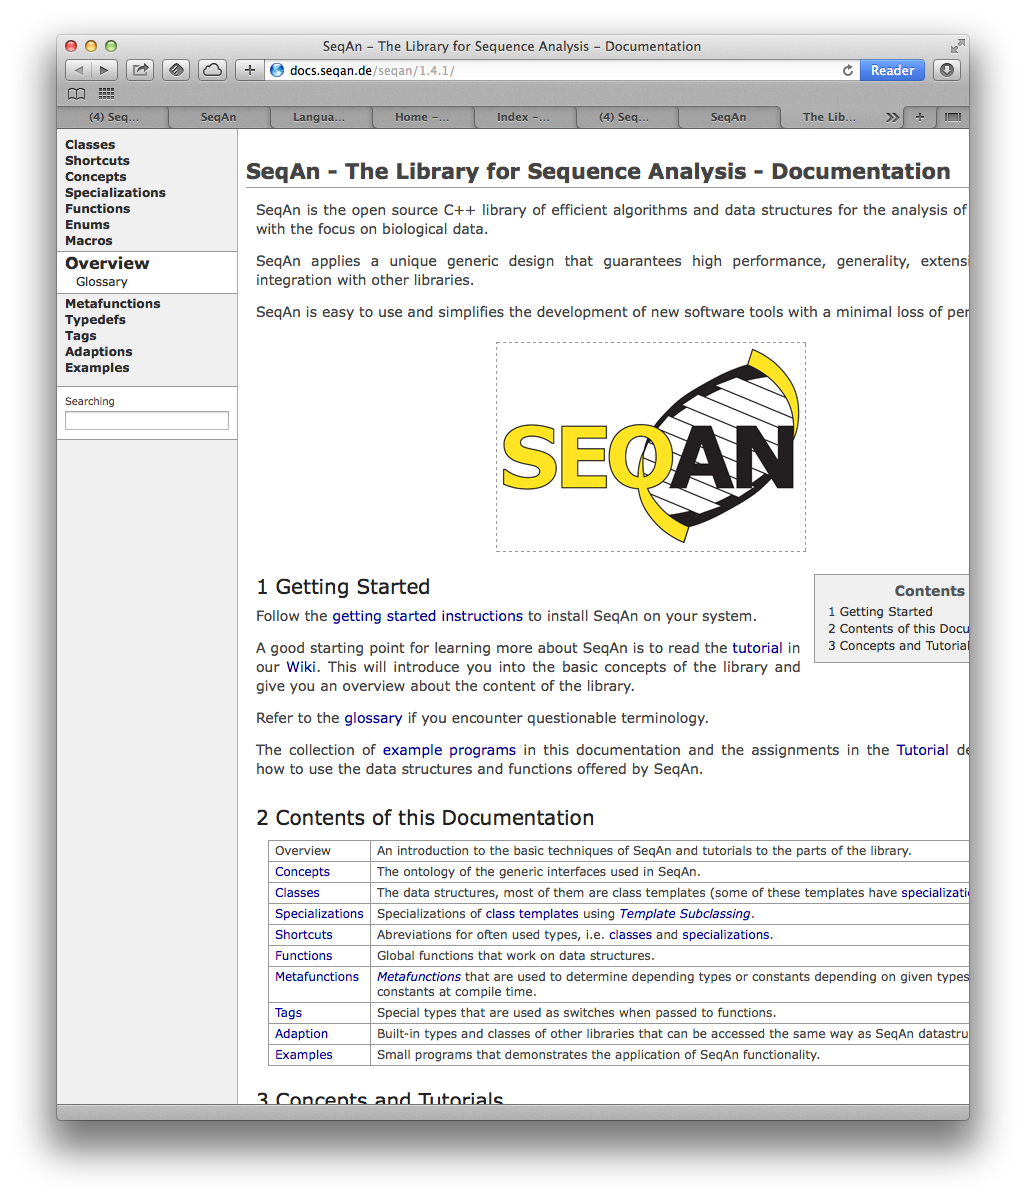
\includegraphics[width=\doxnarrowwidth]{Figures/dox/dox-1_4_1-small-home.png}
    \caption{Seqan-Online-Dokumentation in Version 1.4.1 - Smale Ansicht - Startseite}
    \label{fig:dox-1_4_1-small-home}
\end{figure}

\begin{figure}
  \centering
    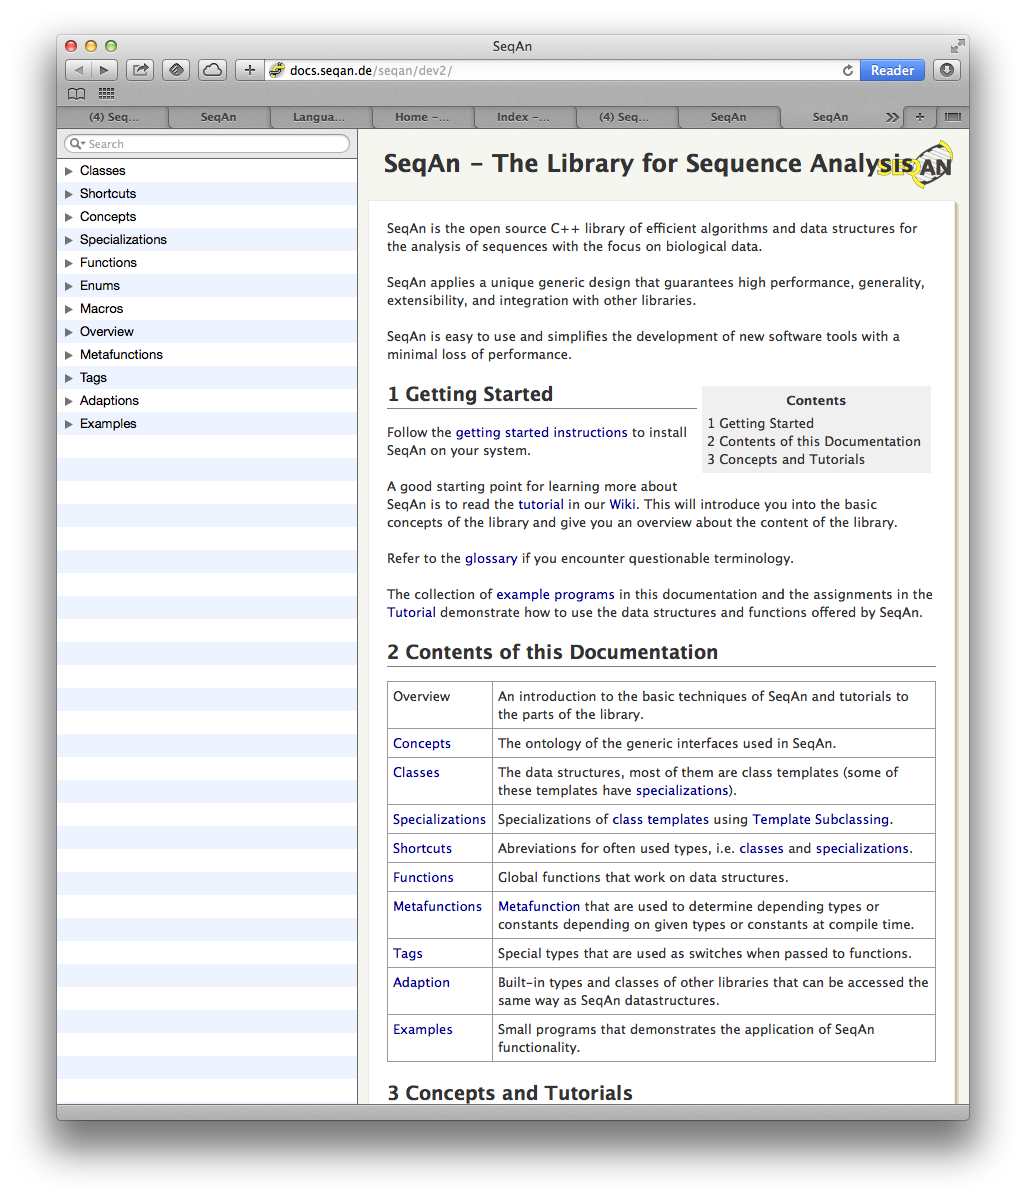
\includegraphics[width=\doxnarrowwidth]{Figures/dox/dox-2_0_0-small-home.png}
    \caption{Seqan-Online-Dokumentation in Version 2.0 - Smale Ansicht - Startseite}
    \label{fig:dox-2_0_0-small-home}
\end{figure}

\begin{figure}
  \centering
    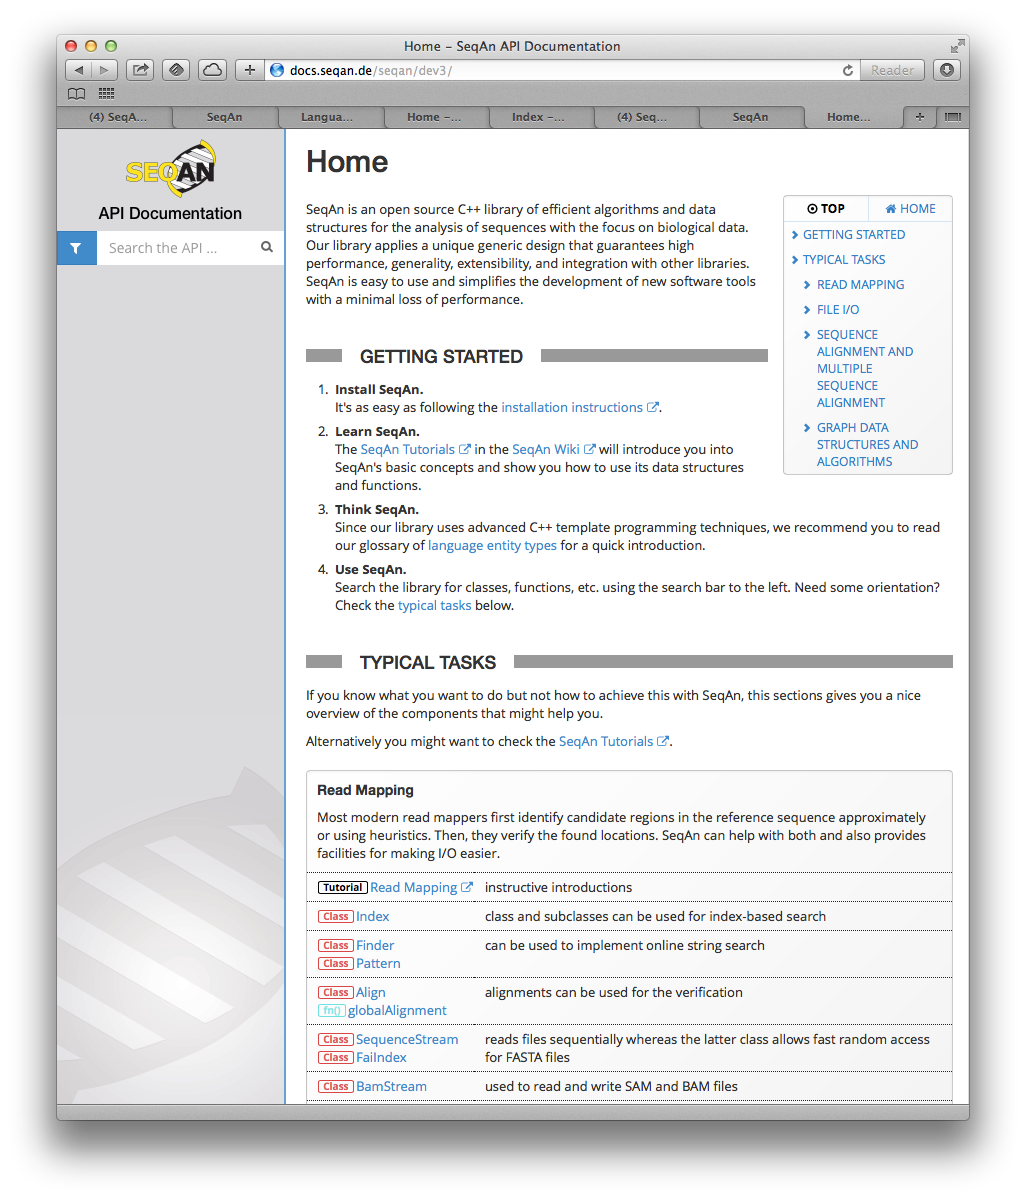
\includegraphics[width=\doxnarrowwidth]{Figures/dox/dox-3_0_0-small-home.png}
    \caption{Seqan-Online-Dokumentation in Version 3.0 - Smale Ansicht - Startseite}
    \label{fig:dox-3_0_0-small-home}
\end{figure}

Donec urna leo, vulputate vitae porta eu, vehicula blandit libero. Phasellus eget massa et leo condimentum mollis. Nullam molestie, justo at pellentesque vulputate, sapien velit ornare diam, nec gravida lacus augue non diam. Integer mattis lacus id libero ultrices sit amet mollis neque molestie. Integer ut leo eget mi volutpat congue. Vivamus sodales, turpis id venenatis placerat, tellus purus adipiscing magna, eu aliquam nibh dolor id nibh. Pellentesque habitant morbi tristique senectus et netus et malesuada fames ac turpis egestas. Sed cursus convallis quam nec vehicula. Sed vulputate neque eget odio fringilla ac sodales urna feugiat.

Donec urna leo, vulputate vitae porta eu, vehicula blandit libero. Phasellus eget massa et leo condimentum mollis. Nullam molestie, justo at pellentesque vulputate, sapien velit ornare diam, nec gravida lacus augue non diam. Integer mattis lacus id libero ultrices sit amet mollis neque molestie. Integer ut leo eget mi volutpat congue. Vivamus sodales, turpis id venenatis placerat, tellus purus adipiscing magna, eu aliquam nibh dolor id nibh. Pellentesque habitant morbi tristique senectus et netus et malesuada fames ac turpis egestas. Sed cursus convallis quam nec vehicula. Sed vulputate neque eget odio fringilla ac sodales urna feugiat.


\begin{figure}
  \centering
    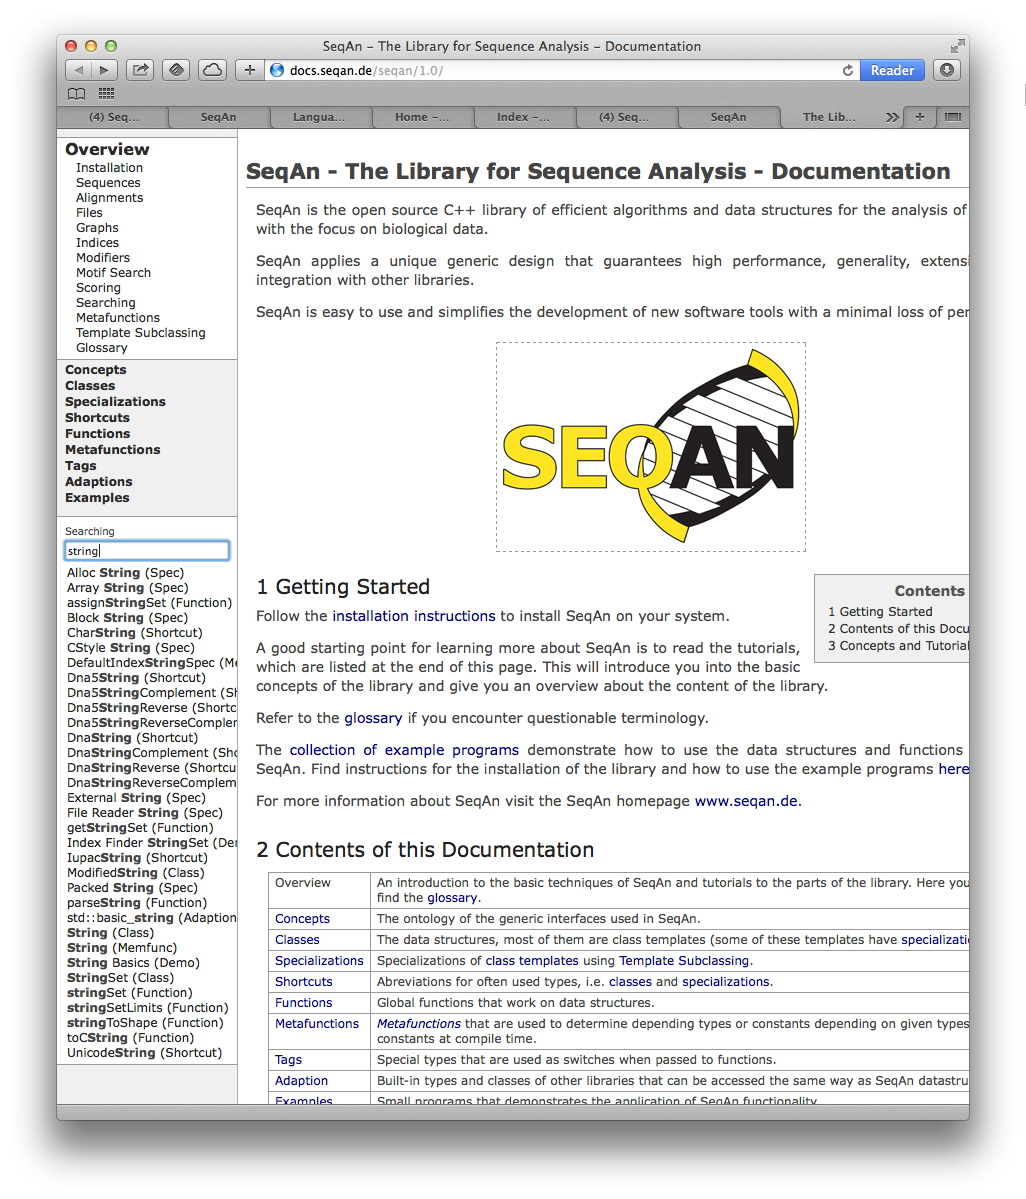
\includegraphics[width=\doxnarrowwidth]{Figures/dox/dox-1_0_0-small-string.png}
    \caption{Seqan-Online-Dokumentation in Version 1.0 - Smale Ansicht - Suche nach ``String''}
    \label{fig:dox-1_0_0-small-string}
\end{figure}

\begin{figure}
  \centering
    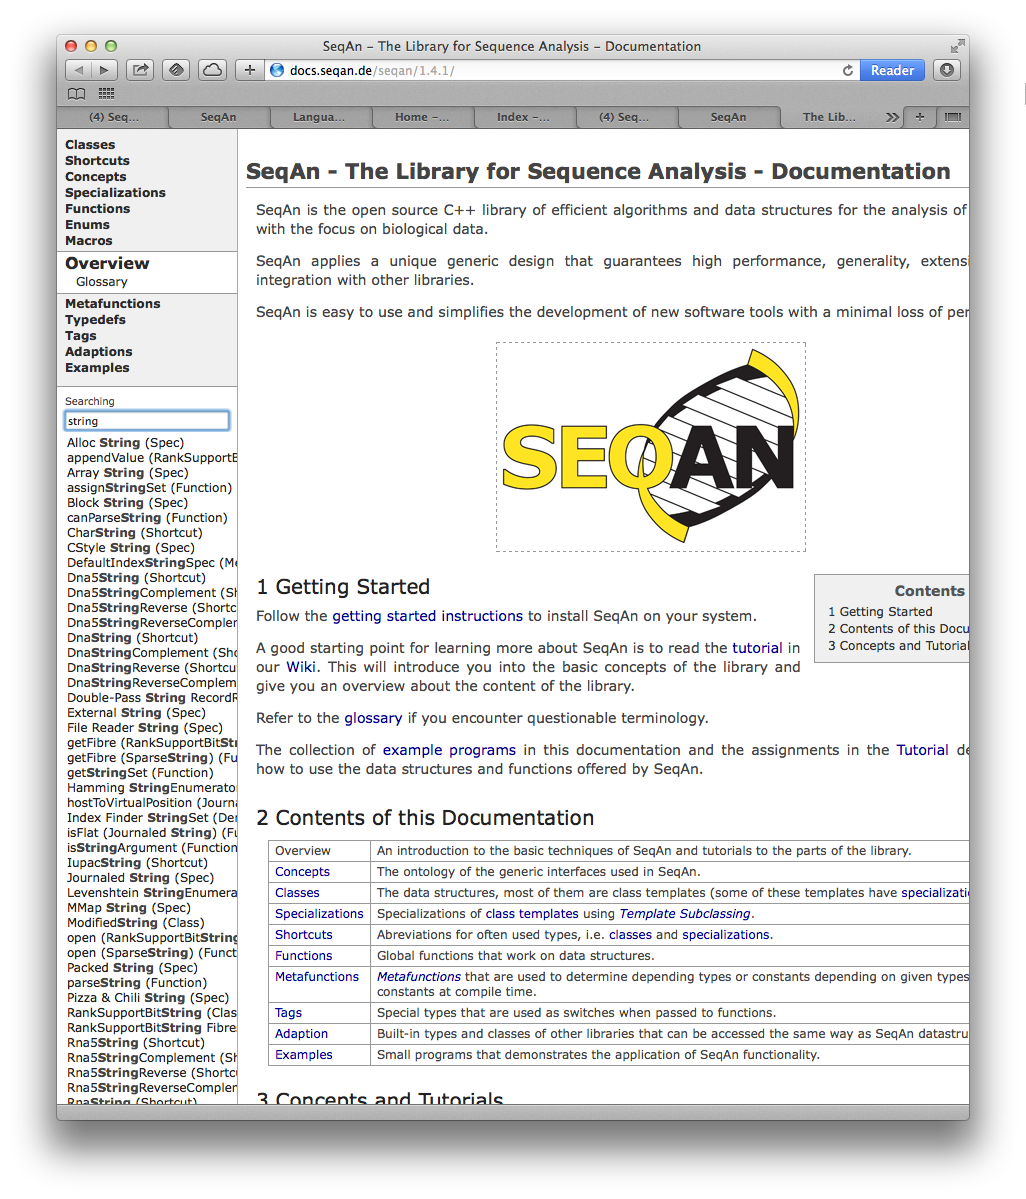
\includegraphics[width=\doxnarrowwidth]{Figures/dox/dox-1_4_1-small-string.png}
    \caption{Seqan-Online-Dokumentation in Version 1.4.1 - Smale Ansicht - Suche nach ``String''}
    \label{fig:dox-1_4_1-small-string}
\end{figure}

\begin{figure}
  \centering
    \includegraphics[width=\doxnarrowwidth]{Figures/dox/dox-2_0_0-small-string.png}
    \caption{Seqan-Online-Dokumentation in Version 2.0 - Smale Ansicht - Suche nach ``String''}
    \label{fig:dox-2_0_0-small-string}
\end{figure}

\begin{figure}
  \centering
    \includegraphics[width=\doxnarrowwidth]{Figures/dox/dox-3_0_0-small-string.png}
    \caption{Seqan-Online-Dokumentation in Version 3.0 - Smale Ansicht - Suche nach ``String''}
    \label{fig:dox-3_0_0-small-string}
\end{figure}

Donec urna leo, vulputate vitae porta eu, vehicula blandit libero. Phasellus eget massa et leo condimentum mollis. Nullam molestie, justo at pellentesque vulputate, sapien velit ornare diam, nec gravida lacus augue non diam. Integer mattis lacus id libero ultrices sit amet mollis neque molestie. Integer ut leo eget mi volutpat congue. Vivamus sodales, turpis id venenatis placerat, tellus purus adipiscing magna, eu aliquam nibh dolor id nibh. Pellentesque habitant morbi tristique senectus et netus et malesuada fames ac turpis egestas. Sed cursus convallis quam nec vehicula. Sed vulputate neque eget odio fringilla ac sodales urna feugiat.

Donec urna leo, vulputate vitae porta eu, vehicula blandit libero. Phasellus eget massa et leo condimentum mollis. Nullam molestie, justo at pellentesque vulputate, sapien velit ornare diam, nec gravida lacus augue non diam. Integer mattis lacus id libero ultrices sit amet mollis neque molestie. Integer ut leo eget mi volutpat congue. Vivamus sodales, turpis id venenatis placerat, tellus purus adipiscing magna, eu aliquam nibh dolor id nibh. Pellentesque habitant morbi tristique senectus et netus et malesuada fames ac turpis egestas. Sed cursus convallis quam nec vehicula. Sed vulputate neque eget odio fringilla ac sodales urna feugiat.

\begin{figure}
  \centering
    \includegraphics[width=\doxnarrowwidth]{Figures/dox/dox-1_0_0-small-string-opened.png}
    \caption{Seqan-Online-Dokumentation in Version 1.0 - Smale Ansicht - Klasse ``String''}
    \label{fig:dox-1_0_0-small-string-opened}
\end{figure}

\begin{figure}
  \centering
    \includegraphics[width=\doxnarrowwidth]{Figures/dox/dox-1_4_1-small-string-opened.png}
    \caption{Seqan-Online-Dokumentation in Version 1.4.1 - Smale Ansicht - Klasse ``String''}
    \label{fig:dox-1_4_1-small-string-opened}
\end{figure}

\begin{figure}
  \centering
    \includegraphics[width=\doxnarrowwidth]{Figures/dox/dox-2_0_0-small-string-opened.png}
    \caption{Seqan-Online-Dokumentation in Version 2.0 - Smale Ansicht - Klasse ``String''}
    \label{fig:dox-2_0_0-small-string-opened}
\end{figure}

\begin{figure}
  \centering
    \includegraphics[width=\doxnarrowwidth]{Figures/dox/dox-3_0_0-small-string-opened.png}
    \caption{Seqan-Online-Dokumentation in Version 3.0 - Smale Ansicht - Klasse ``String''}
    \label{fig:dox-3_0_0-small-string-opened}
\end{figure}








Donec urna leo, vulputate vitae porta eu, vehicula blandit libero. Phasellus eget massa et leo condimentum mollis. Nullam molestie, justo at pellentesque vulputate, sapien velit ornare diam, nec gravida lacus augue non diam. Integer mattis lacus id libero ultrices sit amet mollis neque molestie. Integer ut leo eget mi volutpat congue. Vivamus sodales, turpis id venenatis placerat, tellus purus adipiscing magna, eu aliquam nibh dolor id nibh. Pellentesque habitant morbi tristique senectus et netus et malesuada fames ac turpis egestas. Sed cursus convallis quam nec vehicula. Sed vulputate neque eget odio fringilla ac sodales urna feugiat.

\newgeometry{inner=2cm,outer=1.5cm,top=1.5cm,bottom=1.5cm}
\thispagestyle{empty}
\begin{landscape}
\begin{figure}
        \centering
        \begin{subfigure}[b]{0.38\linewidth}
                \includegraphics[width=\linewidth]{Figures/dox/dox-1_0_0-large-home.png}
                \caption{Version 1.0.0}
                \label{fig:dox-large-home-1.0.0}
        \end{subfigure}
        \hspace{1cm}
        \begin{subfigure}[b]{0.38\linewidth}
                \includegraphics[width=\linewidth]{Figures/dox/dox-1_4_1-large-home.png}
                \caption{Version 1.4.1}
                \label{fig:dox-large-home-1.4.1}
        \end{subfigure}%
        \vskip\baselineskip
        \begin{subfigure}[b]{0.38\linewidth}
                \includegraphics[width=\linewidth]{Figures/dox/dox-2_0_0-large-home.png}
                \caption{Version 2.0.0}
                \label{fig:dox-large-home-2.0.0}
        \end{subfigure}
        \hspace{1cm}
        \begin{subfigure}[b]{0.38\linewidth}
                \includegraphics[width=\linewidth]{Figures/dox/dox-3_0_0-large-home.png}
                \caption{Version 3.0.0}
                \label{fig:dox-large-home-3.0.0}
        \end{subfigure}
        \caption{Diese Abbildung zeigt die verschiedenen Online-Dokumentation-Versionen mit ihrer Startseite.}
        \label{fig:dox-large-home-all}
\end{figure}
\end{landscape}
\restoregeometry

\newgeometry{inner=2cm,outer=1cm,top=1.5cm,bottom=1.5cm}
\thispagestyle{empty}
%\begin{landscape}
\begin{figure}
        \centering
        \begin{subfigure}[b]{0.48\linewidth}
                \includegraphics[width=\linewidth]{Figures/dox/dox-1_0_0-small-home.png}
                \caption{Version 1.0.0}
                \label{fig:dox-small-home-1.0.0}
        \end{subfigure}
        \hfill
        \begin{subfigure}[b]{0.48\linewidth}
                \includegraphics[width=\linewidth]{Figures/dox/dox-1_4_1-small-home.png}
                \caption{Version 1.4.1}
                \label{fig:dox-small-home-1.4.1}
        \end{subfigure}%
        \vskip\baselineskip
        \begin{subfigure}[b]{0.48\linewidth}
                \includegraphics[width=\linewidth]{Figures/dox/dox-2_0_0-small-home.png}
                \caption{Version 2.0.0}
                \label{fig:dox-small-home-2.0.0}
        \end{subfigure}
        \hfill
        \begin{subfigure}[b]{0.48\linewidth}
                \includegraphics[width=\linewidth]{Figures/dox/dox-3_0_0-small-home.png}
                \caption{Version 3.0.0}
                \label{fig:dox-small-home-3.0.0}
        \end{subfigure}
        \caption{Diese Abbildung zeigt die verschiedenen Online-Dokumentation-Versionen in schmaler Breiter mit ihrer Startseite.}
        \label{fig:dox-small-home-all}
\end{figure}
%\end{landscape}
\restoregeometry

Donec urna leo, vulputate vitae porta eu, vehicula blandit libero. Phasellus eget massa et leo condimentum mollis. Nullam molestie, justo at pellentesque vulputate, sapien velit ornare diam, nec gravida lacus augue non diam. Integer mattis lacus id libero ultrices sit amet mollis neque molestie. Integer ut leo eget mi volutpat congue. Vivamus sodales, turpis id venenatis placerat, tellus purus adipiscing magna, eu aliquam nibh dolor id nibh. Pellentesque habitant morbi tristique senectus et netus et malesuada fames ac turpis egestas. Sed cursus convallis quam nec vehicula. Sed vulputate neque eget odio fringilla ac sodales urna feugiat.

\newgeometry{inner=2cm,outer=1.5cm,top=1.5cm,bottom=1.5cm}
\thispagestyle{empty}
\begin{landscape}
\begin{figure}
        \centering
        \begin{subfigure}[b]{0.38\linewidth}
                \includegraphics[width=\linewidth]{Figures/dox/dox-1_0_0-large-string.png}
                \caption{Version 1.0.0}
                \label{fig:dox-large-string-1.0.0}
        \end{subfigure}
        \hspace{1cm}
        \begin{subfigure}[b]{0.38\linewidth}
                \includegraphics[width=\linewidth]{Figures/dox/dox-1_4_1-large-string.png}
                \caption{Version 1.4.1}
                \label{fig:dox-large-string-1.4.1}
        \end{subfigure}%
        \vskip\baselineskip
        \begin{subfigure}[b]{0.38\linewidth}
                \includegraphics[width=\linewidth]{Figures/dox/dox-2_0_0-large-string.png}
                \caption{Version 2.0.0}
                \label{fig:dox-large-string-2.0.0}
        \end{subfigure}
        \hspace{1cm}
        \begin{subfigure}[b]{0.38\linewidth}
                \includegraphics[width=\linewidth]{Figures/dox/dox-3_0_0-large-string.png}
                \caption{Version 3.0.0}
                \label{fig:dox-large-string-3.0.0}
        \end{subfigure}
        \caption{Diese Abbildung zeigt die verschiedenen Online-Dokumentation-Versionen mit dem Suchbegriff ``String''.}
        \label{fig:dox-large-string-all}
\end{figure}
\end{landscape}
\restoregeometry

\newgeometry{inner=2cm,outer=1cm,top=1.5cm,bottom=1.5cm}
\thispagestyle{empty}
%\begin{landscape}
\begin{figure}
        \centering
        \begin{subfigure}[b]{0.48\linewidth}
                \includegraphics[width=\linewidth]{Figures/dox/dox-1_0_0-small-string.png}
                \caption{Version 1.0.0}
                \label{fig:dox-small-string-1.0.0}
        \end{subfigure}
        \hfill
        \begin{subfigure}[b]{0.48\linewidth}
                \includegraphics[width=\linewidth]{Figures/dox/dox-1_4_1-small-string.png}
                \caption{Version 1.4.1}
                \label{fig:dox-small-string-1.4.1}
        \end{subfigure}%
        \vskip\baselineskip
        \begin{subfigure}[b]{0.48\linewidth}
                \includegraphics[width=\linewidth]{Figures/dox/dox-2_0_0-small-string.png}
                \caption{Version 2.0.0}
                \label{fig:dox-small-string-2.0.0}
        \end{subfigure}
        \hfill
        \begin{subfigure}[b]{0.48\linewidth}
                \includegraphics[width=\linewidth]{Figures/dox/dox-3_0_0-small-string.png}
                \caption{Version 3.0.0}
                \label{fig:dox-small-string-3.0.0}
        \end{subfigure}
        \caption{Diese Abbildung zeigt die verschiedenen Online-Dokumentation-Versionen in schmaler Breiter mit dem Suchbegriff ``String''.}
        \label{fig:dox-small-string-all}
\end{figure}
%\end{landscape}
\restoregeometry

Donec urna leo, vulputate vitae porta eu, vehicula blandit libero. Phasellus eget massa et leo condimentum mollis. Nullam molestie, justo at pellentesque vulputate, sapien velit ornare diam, nec gravida lacus augue non diam. Integer mattis lacus id libero ultrices sit amet mollis neque molestie. Integer ut leo eget mi volutpat congue. Vivamus sodales, turpis id venenatis placerat, tellus purus adipiscing magna, eu aliquam nibh dolor id nibh. Pellentesque habitant morbi tristique senectus et netus et malesuada fames ac turpis egestas. Sed cursus convallis quam nec vehicula. Sed vulputate neque eget odio fringilla ac sodales urna feugiat.

\newgeometry{inner=2cm,outer=1.5cm,top=1.5cm,bottom=1.5cm}
\thispagestyle{empty}
\begin{landscape}
\begin{figure}
        \centering
        \begin{subfigure}[b]{0.38\linewidth}
                \includegraphics[width=\linewidth]{Figures/dox/dox-1_0_0-large-string-opened.png}
                \caption{Version 1.0.0}
                \label{fig:dox-large-string-opened-1.0.0}
        \end{subfigure}
        \hspace{1cm}
        \begin{subfigure}[b]{0.38\linewidth}
                \includegraphics[width=\linewidth]{Figures/dox/dox-1_4_1-large-string-opened.png}
                \caption{Version 1.4.1}
                \label{fig:dox-large-string-opened-1.4.1}
        \end{subfigure}%
        \vskip\baselineskip
        \begin{subfigure}[b]{0.38\linewidth}
                \includegraphics[width=\linewidth]{Figures/dox/dox-2_0_0-large-string-opened.png}
                \caption{Version 2.0.0}
                \label{fig:dox-large-string-opened-2.0.0}
        \end{subfigure}
        \hspace{1cm}
        \begin{subfigure}[b]{0.38\linewidth}
                \includegraphics[width=\linewidth]{Figures/dox/dox-3_0_0-large-string-opened.png}
                \caption{Version 3.0.0}
                \label{fig:dox-large-string-opened-3.0.0}
        \end{subfigure}
        \caption{Diese Abbildung zeigt die verschiedenen Online-Dokumentation-Versionen mit der geöffneten Klasse \textit{String}.}
        \label{fig:dox-large-string-opened-all}
\end{figure}
\end{landscape}
\restoregeometry

\newgeometry{inner=2cm,outer=1cm,top=1.5cm,bottom=1.5cm}
\thispagestyle{empty}
%\begin{landscape}
\begin{figure}
        \centering
        \begin{subfigure}[b]{0.48\linewidth}
                \includegraphics[width=\linewidth]{Figures/dox/dox-1_0_0-small-string-opened.png}
                \caption{Version 1.0.0}
                \label{fig:dox-small-string-opened-1.0.0}
        \end{subfigure}
        \hfill
        \begin{subfigure}[b]{0.48\linewidth}
                \includegraphics[width=\linewidth]{Figures/dox/dox-1_4_1-small-string-opened.png}
                \caption{Version 1.4.1}
                \label{fig:dox-small-string-opened-1.4.1}
        \end{subfigure}%
        \vskip\baselineskip
        \begin{subfigure}[b]{0.48\linewidth}
                \includegraphics[width=\linewidth]{Figures/dox/dox-2_0_0-small-string-opened.png}
                \caption{Version 2.0.0}
                \label{fig:dox-small-string-opened-2.0.0}
        \end{subfigure}
        \hfill
        \begin{subfigure}[b]{0.48\linewidth}
                \includegraphics[width=\linewidth]{Figures/dox/dox-3_0_0-small-string-opened.png}
                \caption{Version 3.0.0}
                \label{fig:dox-small-string-opened-3.0.0}
        \end{subfigure}
        \caption{Diese Abbildung zeigt die verschiedenen Online-Dokumentation-Versionen in schmaler Breiter mit der geöffneten Klasse \textit{String}.}
        \label{fig:dox-small-string-opened-all}
\end{figure}
%\end{landscape}
\restoregeometry
\end{comment}



\glsresetall

\chapter{Einleitung}

Dieses Kapitel befasst sich mit der Motivation, die sich hinter der Erforschung der API-Usability von SeqAn verbirgt. Es beantwortet die Fragen, was API-Usability überhaupt ist und weshalb sie so wichtig ist. Anschließend wird erläutert, worum es sich bei SeqAn exakt handelt, und welchen Zweck SeqAn erfüllt. Abgeschlossen wird dieses Kapitel mit der Vorstellung, der in dieser Arbeit verwendeten \glslink{gtm}{Grounded Theory Forschungsmethode}.



\section{Motivation}
\label{sec:motivation}

Diese Arbeit verfolgt das Ziel, die Benutzerfreundlichkeit\footnote{Die Übersetzung des englischen Begriffs \textit{Usability} ins Deutsche ist kompliziert. Nach dem Inhalt der DIN EN ISO 9241 müsste man den Begriff ``Gebrauchstauglichkeit'' verwenden, wohingegen --- nach meinem persönlichen Eindruck --- der Begriff ``Benutzerfreundlichkeit'' von der deutschen Bevölkerung besser verstanden und vorgezogen wird. Ich werde daher alle drei Begriffe synonym verwenden. In \sref{sec:def-usability} gehe etwas genauer auf dieses Problem ein.} (engl. \textit{Usability}) der Softwarebibliothek \textit{SeqAn} im Rahmen einer explorativen empirischen Fallstudie zu verbessern. Wie ich\footnote{Diese Arbeit ist in der Ich-Form verfasst. Die Begründung für diesen Entschluss ist in der verwendeten Forschungsmethode begründet, die ich ab Seite \pageref{sec:gtm} vorstelle.} im \hyperref[sec:forschungsstand]{nächsten Kapitel} noch erläutern werde, ist die klassische Usability-Verbesserung von Endanwender-Programmen bereits gut erforscht und, für sich genommen, lediglich anspruchsvolles Handwerk. Anders sieht es aus, wenn beispielsweise neuartige Bedienkonzepte entwickelt, evaluiert und verbessert werden sollen.

Im Falle von SeqAn sind gleich zwei Aspekte interessant:
\begin{enumerate}
  \item SeqAn ist keine Anwendersoftware, mit der durch eine \gls{gui} interagiert wird, sondern eine Softwarebibliothek, die mittels einer weiter unten definierten \glslink{api}{Applikationsprogrammierschnittstelle (engl. \textit{application programming interface}, kurz: API)} verwendet wird.
      \\Oder anders ausgedrückt: Während man in ``normalen Programmen'' herum klickt, muss man bei SeqAn mit Hilfe einer selbst gewählten Entwicklungsumgebung programmieren.
  \item SeqAn löst keine Informatik-eigenen Probleme wie Persistierung oder Logging, sondern bietet Funktionen zur Lösung von Problemen aus der Bioinformatik an. 
\end{enumerate}

Schaut man genauer hin, ergeben sich drei anspruchsvolle, zu lösende Problemfelder:
\begin{enumerate}
  \item Im Bereich der Forschung wurde der Usability von APIs weit weniger Aufmerksamkeit geschenkt, als der Usability von Endanwender-Programmen \citep{Grill:2012jm}. Erst seit Kurzem hat das Interesse an API-Forschung wegen des ansteigenden Gebrauchs von APIs zugenommen \citep{Daughtry:2009be}. 2009 fand das erste und bis dato einzige Treffen der \textit{Special Interest Group} ``API Usability'' auf der CHI 2009\footnote{\url{http://www.chi2009.org}} statt \citep{Daughtry:2009dv}. Wie ich im \hyperref[sec:forschungsstand]{nächsten Kapitel} zeigen werde, ist der Korpus an empirischer Grundlagenforschung klein und es fehlen umfassende wissenschaftliche Literaturstudien.
  \item SeqAns Alleinstellungsmerkmal ist seine kompromisslose Effizienz. Um diese zu erreichen, basiert SeqAn auf dem sehr anspruchsvollen Programmierparadigma \textit{Templatemetaprogrammierung}\footnote{Dass es sich bei der Templatemetaprogrammierung um die Hauptursache für SeqAns fragliche Usability handeln würde, schien allen Beteiligten mehr oder minder klar zu sein. Wenn ich im diesen Sinne von der Templatemetaprogrammierung spreche, handelt es sich allerdings um einen Vorgriff auf mein in dieser Arbeit vorgestelltes Forschungsergebnis. Bewusst habe ich auch andere Ursachen in Betracht gezogen, die ich ebenfalls in dieser Arbeit vorstelle.}, zu der es keinerlei Erkenntnisse in Bezug auf die Usability gibt.
  \item Das Spektrum an Anwendern von SeqAn ist breit und reicht vom professionellen Entwickler bis hin zum Biologen mit minimalen Programmierfertigkeiten. Letzterer gehört der Gruppe der \textit{Endanwender-Programmierer} an \citep{Tisdall:2001td}. Die Forschung im Bereich der Endanwender-Programmierung hat sich allerdings vornehmlich auf visuelle Programmiersprachen\footnote{Definition nach \cite{schiffer1998visuelle}: ``Eine visuelle Sprache ist eine formale Sprache mit visueller Syntax oder visueller Semantik und dynamischer oder statischer Zeichengebung.''} konzentriert \citep{Ko:2011el,Gieselmann:-Uisl6hs}, zu der die von SeqAn verwendete Programmiersprache C{}\verb!++! nicht gehört.
\end{enumerate}

Im Folgenden möchte ich klären, was Bioinformatik überhaupt ist, weshalb Bioinformatiker APIs benötigen und welchen Nutzen APIs im Speziellen wie auch im Allgemeinen haben. 



\subsection[Bedeutung der Bioinformatik]{Was ist überhaupt Bioinformatik?}

Die Bioinformatik ist eine interdisziplinäre Wissenschaft, die Methoden der Informatik auf biologische Daten und Fragestellungen anwendet \citep{Gibas:2002wk}. Quellen für biologische Daten sind dabei Sequenzierungen von Genomen, Expressionsprofile von Proteinen, Strukturaufklärung von Proteinen und Interaktionen zwischen Biomolekülen wie Proteinen, RNAs und niedermolekularen Verbindungen \citep{Rarey:E0TiqhGO}.

Mit jedem Jahr werden immer größere Datenmengen produziert. Allein das menschliche Genom umfasst etwa 3 Milliarden Basenpaare\footnote{Das Basenpaar beschreibt ein Paar Nukleobasen. Die wohl bekanntesten Basen sind \textbf{A}denin, \textbf{C}ytosin, \textbf{G}uanin und \textbf{T}hymin. Sie treten bei der DNA als die Paare A-T und C-G auf.} \citep{Tisdall:2001td}. Deutlich kleinere Genome können bei Auswertungszwischenschritten bereits mehrere Terabytes große Datenmengen verursachen \citep{Reinert:tg}. Der Zuwachs an Daten hat mittlerweile ein exponentielles Wachstum angenommen. Für die Vorbereitung, Auswertung und Analyse dieser Datenmassen werden Werkzeuge benötigt, die durch die Bioinformatik bereitgestellt werden \citep{Gibas:2002wk}.

Das Hauptaufgabengebiet der Bioinformatik liegt in der Sequenzanalyse. Darunter wird die Analyse von biomolekularen Sequenzen, wie der DNA, RNA oder Aminosäuren verstanden. Diesem Vorgehen liegt die Beobachtung zu Grunde, dass eine hohe Sequenzähnlichkeit für gewöhnlich eine signifikante, funktionale oder strukturelle Ähnlichkeit impliziert \citep{AlgorithmenundDate:2011wx}. Zu den ersten Bioinformatikern gehören \cite{Needleman:1970vq}, auf deren Algorithmus heute noch viele Methoden zur Sequenzanalyse basieren \citep{hansen2013bioinformatik}.

In den vergangenen Jahren sind die Kosten für Hochdurchsatz-Sequenzierungsverfahren, die auch als \textit{Next Generation Sequencing} (NGS) bezeichnet werden, rapide gefallen. Dies führt zu einer extrem schnellen Entwicklung im Feld der Bioinformatik \citep{Li:2012fl}. So haben beispielsweise \cite{Alexander:2012fb} ein Verfahren entwickelt, das einen potentiell vorliegenden Schilddrüsenkrebs ohne chirurgischen Eingriff mit hoher Wahrscheinlichkeit ausschließen kann. Dieses Verfahren kann Patienten die unnötige Entfernung ihrer Schilddrüse und die damit einhergehende lebenslange Hormontherapie ersparen.

Bereits heute ist die Sequenzierung eines menschlichen Genoms für weniger als 1.000\$ zu haben \citep{Young:2014tl}; in wenigen Jahren wird die 100\$-Grenze unterschritten sein \citep{Reinert:tg}. Diese Entwicklung ermöglicht vollkommen neue Anwendungsformen, z.B. in den Bereichen der personalisierten Medizin, Metagenomik und der klinischen Forschung \citep{Reinert:tg}. SAP-Mitgründer Dietmar Hopp spricht sogar davon, ``dass Life Sciences die nächste Welle nach der Informationsverarbeitung sein wird'' und hat bereits mehr als eine Milliarde Euro in den Bereich der Biotechnologie investiert \citep{Ziegler:2015tt}. Auf staatlicher Ebene werden, teil bereits seit Jahren, nationale Großprojekte verfolgt \citep{Young:2014tl}. Ein solches ist das \textit{Genomics England} Projekt\footnote{\url{http://www.genomicsengland.co.uk}}, das durch den staatlichen Gesundheitsanbieter \textit{National Health Service}\footnote{\url{http://www.nhs.uk}} geplant wird. Dieses Projekt sieht vor, bis 2017 die Gendaten von insgesamt 100.000 Patienten vollständig zu erfassen und in einem ersten Schritt für die Erforschung von seltenen Krankheiten, Krebs und Infektionskrankheiten zu nutzen.

Die auch als \textit{Bioethik} bezeichnete ethische Auseinandersetzung setzt sich in einer überraschenden Breite sowohl mit ganz grundsätzlichen \citep{Bouvet:2006ig}, wie auch methodischen \citep{Vayena:2015kk}, als auch didaktischen \citep{Gasparich:2014eg} Fragestellungen auseinander. Auch hoch aktuelle Themen, wie der immer noch andauernde Ebola-Ausbruch in Westafrika im Frühjahr 2014, sind Gegenstand des ethischen Diskurses \citep{Blais:2015tw}. Auf nationaler Ebene beschäftigt sich der Ethikrat der Bundesrepublik Deutschland auch mit der Bioethik\footnote{\url{http://www.ethikrat.org/veranstaltungen/anhoerungen/praediktive-genetische-diagnostik-multifaktorieller-erkrankungen}}. Auf internationaler Ebene ist dafür das bereits 1993 eingerichtete \textit{International Bioethics Committee}\footnote{\url{http://www.unesco.org/new/en/social-and-human-sciences/themes/bioethics/international-bioethics-committee/}} zuständig. 




\subsection[Bioinformatik und Programmieren]{Warum müssen Bioinformatiker und Biologen programmieren?}

Wie bereits erwähnt, entwickelt sich die Bioinformatik rasant. Während die Datenmengen stetig steigen, entstehen immer wieder neue Algorithmen und Hypothesen \citep{Letondal:2006dy}. Diese Entwicklung führt dazu, dass Probleme formuliert werden, für deren Lösung es noch keine \citep{Tisdall:2001td} oder nur unzureichende \citep{Letondal:2006dy} grafische Werkzeuge existieren.

Während es zu den fachbedingten Tätigkeiten der Bioinformatik gehört, Code schreiben zu müssen, trifft dies nun auch auf Biologen zu. Anders wäre es ihnen nicht möglich, neuartige Hypothesen zu überprüfen \citep{Letondal:2006dy,Tisdall:2001td}. Damit bilden Biologen klassische Vertreter der Endanwender-Programmierer.

Unabhängig von verfügbaren grafischen Werkzeugen gibt es einen immensen Automatisierungsbedarf in Form von Stapelverarbeitungsskripten (engl. \textit{batch scripts}) und \textit{Workflows}. Abgesehen von der geringeren Fehlerquote wird Automatisierung durch den enormen Zeitgewinn motiviert: Während die händische Auswertung von Gen-Abschnitten einen Monat oder mehr beanspruchen kann, kann ein in zwei Wochen entwickeltes Skript dieselbe Arbeit in 30 Minuten leisten \citep{Tisdall:2001td}. Bedenkt man das Alter der Quelle und die fortschreitende Entwicklung von Informatik und Bioinformatik, wird dieser Zeitgewinn sicherlich gewachsen sein.

Die Bioinformatik verfügt bereits über ein großes Repertoire an Algorithmen, die Lösungsbestandteile neuartiger Probleme darstellen. Existierende Implementierungen werden über Softwarebibliotheken, Frameworks, etc. bereitgestellt; sie wiederzuverwenden verringert die Anzahl an produzierten Defekten in den entwickelten Werkzeugen und erhöht zugleich die Effizienz der Arbeit.





\subsection[Relevanz von API-Usability]{Warum ist die Benutzerfreundlichkeit von APIs überhaupt so wichtig?}

Moderne Softwareentwicklung macht ausgiebig Gebrauch von dem Prinzip der Wiederverwendung \citep{Piccioni:2013uq}. Wiederverwendbarer Code wird am häufigsten in Form von \textit{Frameworks} und \textit{Softwarebibliotheken} bereitgestellt \citep{Henning:2007kg,Jeong:kf}, wobei letztere am häufigsten von Anwendern genutzt werden \citep{Feilkas:dg}. Die Nutzung von existierendem qualitativem Code hat gegenüber der Neuimplementierung potentiell die Vorteile geringerer Kosten sowie eine höhere Sicherheit und Stabilität \citep{Stylos:2009ts}.

Der Zugriff auf eine Softwarebibliothek wird über eine API realisiert. Weil es sich dabei um die Schnittstelle zwischen Anwender und Softwarebibliothek handelt, ist die Usability ein fundamentales Ziel bei der Entwicklung der API \citep{Piccioni:2013uq}.

APIs sind schwer zu verwenden \citep{Stylos:2006ji} und schwer zu erlernen, weil nicht nur die einzelne Klasse, sondern auch das Zusammenspiel der Klassen wichtig ist \citep{Bruch:2006bv}. Das gilt sogar für etablierte APIs wie dem Java Development Kit\footnote{\url{http://www.oracle.com/technetwork/java/javase}} \citep{Stylos:2009gc}. In besonders schweren Fällen kann der Verwender einer API sogar so stark ausgebremst werden, dass er schneller ohne die Verwendung der API gewesen wäre \citep{Stylos:2007ip}.

Eine schlechte API-Usability verringert die Produktivität und Codequalität \citep{Zibran:2011fx} bei der Entwicklung von Programmen mit Hilfe dieser API. Inzwischen ist eine \textit{API-Ökonomie} entstanden \citep{Hulsenbusch:2014wr}, bei der sich die Benutzerfreundlichkeit natürlich auch auf die Wettbewerbsfähigkeit auswirkt \citep{Stylos:2009ts}. Ist eine API zu schwer zu erlernen, wechseln die Anwender eben auf eine andere API \citep{sunshine2014searching}. Aus humanistischer und arbeitspsychologischer Sicht wirkt sich die Arbeit mit einem benutzer\textit{un}freundlichen System negativ auf Wohlbefinden und Motivation aus \citep{Sarodnick:2006vc}.

\subsection[Nutzen von API-Usability]{Lohnt sich wirklich der Aufwand zur Verbesserung der Benutzerfreundlichkeit von APIs?}

Diese Frage ist nicht nur für die Leser und Geldgeber dieser Arbeit sowie für die Autoren von APIs von Wichtigkeit, sondern auch für mich selbst. Schließlich stand ich vor der Wahl, eine Promotion über einen Zeitraum von drei oder mehr Jahren zu verfolgen und fachlich wie auch motivatorisch zu meistern.

Etablierte APIs werden tausendfach häufiger verwendet als entwickelt \citep{Ellis:2007kv}. Die Mehrkosten für die Autoren von APIs sind vielfach kleiner als der Schaden, den benutzerunfreundliche APIs ihren Anwendern anrichten \citep{Henning:2007kg}. Die Verantwortung für eine benutzerfreundliche API liegt also klar bei seinen Autoren. Außerdem ist eine einmal veröffentlichte API quasi ewig --- es existiert also nur eine Chance, sie korrekt zu entwerfen \citep{Bloch:2006jk}.

Wird die API-Usability nicht explizit beim Entwurf beachtet, ist sie weiter nichts als ein extrem unwahrscheinlicher Zufall \citep{Stylos:2009ts}. Bereits kleine und unschuldig anmutende Mängel tendieren dazu, sich negativ in überproportionalen Größenordnungen auszuwirken \citep{Henning:2009hz}. \cite{Stylos:2007ip} bezeichnen dies trefflich als ``death by 1000 paper cuts''.

Für die besonders anspruchsvolle Anwendergruppe der Endanwender-Programmierer, zu denen auch Biologen \citep{Tisdall:2001td} und teilweise auch Bioinformatiker \citep{Letondal:2006dy} gehören, ist das Schadpotential besonders groß. Schließlich verfügt diese Gruppe über weit weniger Erfahrung im Bereich der Softwaretechnik und kann Usability-Probleme weniger gut kompensieren, als ihre erfahreneren Kollegen \citep{Shaft:1998tc}.

Die Verbesserung der API-Usability ist möglich und wurde in einigen Studien gezeigt \citep{Letondal:2006dy,Grill:2012jm,Tenny:2011jp,Piccioni:2013uq}. Wie meine, im \sref{sec:forschungsstand} vorgestellte Literaturrecherche zeigt, ist der Wissensstand in diesem Bereich jedoch noch stark fragmentiert. Ein Grund dafür ist --- neben der Vernachlässigung von API-Usability zu Gunsten der klassischen Usability --- die Vielzahl an Einflussfaktoren, zu denen, neben der API selbst, auch die dazugehörige Dokumentation, die gewählte Programmiersprache und Entwicklungswerkzeuge gehören \citep{Stylos:2008jt}.

\subsection{Synthese und Zusammenfassung}

APIs bilden die Schnittstelle zu wiederverwendbarem Code. Ohne diese Schnittstelle ist der Nutzer gezwungen, Code zu duplizieren, was zu einer ganzen Fülle von Nachteilen führt \citep{Spinellis:2006tj}. Glücklicherweise wird wiederverwendbarer Code häufig in Form von Softwarebibliotheken gekapselt und durch APIs zugänglich gemacht.

Eine benutzerunfreundliche API führt zu einer Reihe von Problemen, die sich negativ auf die ganze Spannbreite von persönlichen bis hin zu wirtschaftlichen Erfolgsfaktoren auswirken. Um diesen potentiellen Schaden abzuwenden, müssen sich die Entwickler einer API aktiv für dessen Usability einsetzen. Bei ihnen liegt aus fachlichen und ökonomischen Gründen die Verantwortung dafür. Leider ist diese Anforderung leichter formuliert als erfüllt, denn die Forschung im Bereich der API-Usability steht der Forschung im Bereich der klassischen Usability um einiges nach. Hinzu kommt, dass es an umfassenden wissenschaftlichen Literaturstudien fehlt.

Die Bioinformatik entwickelt Werkzeuge, mit denen Problemstellungen gelöst werden können, die unter anderem zu einem besseren Verständnis von Krankheiten und deren Heilungsmöglichkeiten führen. Dazu greifen Bioinformatiker auf Softwarebibliotheken zurück. Eine solche Softwarebibliothek ist SeqAn, die das Leben ihrer Anwender durch den intensiven Gebrauch des Programmierparadigmas Templatemetaprogrammierung nicht unbedingt leicht macht. Zu allem Überfluss ist dieses Paradigma in Bezug auf seine Benutzerfreundlichkeit vollkommen unerforscht.

Die allgemein formulierten Nachteile einer schlechten API-Usability bedeuten für den Bereich der Bioinformatik, dass die Forschung im besten Fall ausgebremst wird. Eine gute API-Usability hingegen erlaubt es nicht nur Bioinformatikern effizienter zu arbeiten, sondern kann --- unter Berücksichtigung von Erkenntnissen aus der Endanwender-Softwaretechnik --- Biologen in den Zustand versetzen, sich ebenfalls bioinformatisch zu betätigen. Dass dies tatsächlich möglich ist, konnte in einer Arbeit gezeigt werden \citep{Letondal:2006dy}, die ich im \sref{sec:letondal} vorstelle.

\bigskip

Als Forscher und Autor dieser Dissertation beschäftige ich mich also mit den Aufgaben, (1) eine umfassende wissenschaftliche Literaturstudie durchzuführen, (2) die Usability von Templatemetaprogrammierung im Allgemeinen und von SeqAn im Speziellen empirisch zu erforschen, (3) die besonderen Anforderungen von Endanwender-Programmierern zu berücksichtigen, (4) Vorschläge für die Verbesserung der Usability von SeqAn zu formulieren und (5) diese umzusetzen.





\section{Definitionen}
\label{sec:definitions}

An dieser Stelle möchte ich knapp auf Übersetzungsschwierigkeiten vom Englischen ins Deutsche eingehen: Bekanntermaßen ist die Informatik durch englischsprachige Begriffe geprägt. Außerdem wird der mit Abstand größte Teil wissenschaftlicher Veröffentlichungen im Bereich der Informatik in englischer Sprache verfasst. Für viele englische Begriffe gibt es etablierte Übersetzungen (z.B. \textit{interface} \& \textit{Schnittstelle}). Andere Begriffe lassen sich hingegen nur mühselig (z.B. \textit{usability} \& \textit{Gebrauchstauglichkeit}/\textit{Nutzbarkeit}/\textit{Benutzerfreundlichkeit}) oder gar missverständlich (z.B. \textit{framework} \& \textit{Rahmenwerk}) übersetzen.

Aus diesen Gründen werde ich für den Rest dieser Arbeit nach Möglichkeit den deutschen Begriff verwenden. Würde eine Übersetzung jedoch unnötig kompliziert sein oder gar missverstanden werden können, verwende ich den englischen Begriff. Wenn es sich um kein direktes Zitat handelt, schreibe ich englische Substantive mit großem Anfangsbuchstaben und verwende den sächlichen Artikel. Bei Abkürzungen, die sowohl den englischen als auch deutschen Begriff beschreiben (z.B. \textit{API}), nutze ich den Artikel des deutschen Begriffs (z.B. \textit{die API}). Von diesen Vereinbarungen mache ich gleich bei der folgenden ersten Definition Gebrauch.

\bigskip

Basierend auf existierenden Definitionen \citep{dekel2011increasing,Tenny:2011jp,zibran2008makes,Zibran:2011fx,McLellan:1998cu,Henning:2007kg,Robillard:2009cs,Stylos:2009ts}, definiere ich \textit{API} wie folgt:
\begin{description}
  \item Eine \glslink{api}{\textit{Applikationsprogrammierschnittstelle} (engl. \textit{application programming interface}, kurz: \textit{API})} ist eine Schnittstelle zwischen Anwender und dem der Schnittstelle zu Grunde liegenden Code, der eine bestimmte Funktionalität implementiert. Eine API liegt in Gestalt einer Softwarebibliothek, eines Framework, SDKs, Toolkits, etc. vor, umfasst alle dazu in Verbindung stehenden Ressourcen (Installationsdateien, Dokumentation, etc.) und definiert dabei eine Dienstleistung, welche die Komplexität der Implementierung mittels Abstraktion versteckt. Bei APIs handelt es sich um eine fortgeschrittene Form der Code-Wiederverwendung, die den Bau komplexer Software ermöglicht.
\end{description}

\bigskip

Obwohl es eine Reihe Veröffentlichungen im Bereich der API-Usability gibt, hat sich erstaunlicherweise noch keine grundlegende einheitliche Terminologie für die folgenden drei relevanten Parteien entwickelt. Einige Arbeiten verwenden zumindest den Begriff \textit{API user} --- ohne ihn jemals explizit eingeführt zu haben. Ich schlage daher folgende Begriffe vor:

\begin{description}
  \item Ein \textit{API-Entwickler} (engl. \textit{API developer} bzw. \textit{API designer}) ist eine Person, die an der Entwicklung einer API beteiligt ist. Neben der eigentlichen Programmierung gehören auch Konzeption, Entwurf oder Wartung in ihre Arbeitsbereiche.
  \item Ein \textit{API-Anwender} (engl. \textit{API user}) ist eine Person, die eine oder mehrere \glslink{api}{APIs} nutzt, um ein Problem programmatisch zu lösen.
\end{description}

\bigskip

Da sich diese Arbeit mit einer Software befasst, die nicht ausschließlich von professionellen Softwareentwicklern genutzt wird, muss sie sich auch mit der Endanwender-Softwaretechnik auseinandersetzen. \sref{sec:euse} befasst sich näher mit diesem Thema. An dieser Stelle möchte ich lediglich den Begriff des \textit{Endanwender-Programmierers} herausgreifen.

\begin{description}
  \item Ein \textit{Endanwender-Programmierer} (engl. \textit{end-user programmer}) ist eine Personen, deren Ziel --- im Gegensatz zum professionellen Programmierer --- nicht das Programmieren selbst ist. Stattdessen ist Programmieren für sie ein ``notwendiges Übel'' zur Erreichung ihres Ziels innerhalb ihrer Expertendomäne.
\end{description}

\bigskip

Auf den Bereich der API-Usability übertragen, können API-Entwickler und API-Anwender um eine weitere Rolle ergänzt werden:

\begin{description}
  \item Ein \textit{API-Endanwender} (engl. \textit{API end-user}) ist ein spezieller Endanwender-Programmierer, der eine API zum Erreichen seines Ziels nutzt.
\end{description}

Abhängig vom Kontext verwende ich den Begriff \textit{API-Anwender} als Überbegriff für \textit{API-Anwender} und \textit{API-Endanwender} --- also als undifferenzierte Bezeichnung für alle Anwender einer API.

\begin{comment}
\bigskip

Abschließend definiere ich noch die Rolle, die in der klassischen Usability-Forschung die sicherlich wichtigste Partei darstellt:

\begin{description}
  \item Ein \textit{Produkt-Anwender} bzw. \textit{Anwender} (engl. \textit{user}) ist eine Person, die durch API-Anwender erstellte Programme nutzt.
\end{description}

Es ist wichtig, diese Gruppe explizit zu benennen, da sie die Folgen einer guten bzw. schlechten API-Usability spürt. Bei APIs für grafische Benutzeroberflächen wie Swing, QT oder SWT ist dies besonders der Fall, da eine inkorrekte Verwendung dieser APIs sich besonders schnell in der grafischen Benutzeroberfläche des Endanwender-Programms bemerkbar macht.
\end{comment}

\bigskip

Wie ich weiter unten noch erläutern werde, ist die dieser Arbeit zu Grunde liegende Forschungsmethode die \textit{\gls{gtm}}. Diese Methode verwendet den englischen Begriff \textit{Code}, der leider mit dem Code-Begriff aus der Informatik kollidiert. Für den Rest dieser Arbeit werde ich für den GTM-Code-Begriff \textit{Kode} bzw. \textit{Konzept} und für den Informatik-Code-Begriff \textit{Code} bzw. \textit{Quellcode} benutzen.

Leider steht der GTM-Konzept-Begriff wiederum im Konflikt mit dem Konzept-Begriff aus der Templatemetaprogrammierung. Daher werde ich für den GTM-Konzept-Begriff \textit{Konzept} und für den Templatemetaprogrammierungs-Konzept-Begriff \textit{Concept} verwenden. Die Eselsbrücke lautet: Für nicht-technische Gebiete verwende ich die deutsche Übersetzung und für technische Konfliktbegriffe das englische Wort im Original.




\section{SeqAn}

SeqAn\footnote{\textbf{Seq}uenz-\textbf{An}alyse} ist eine quelloffene C{}\verb!++!-Softwarebibliothek, die von Andreas Gogol-Döring im Rahmen seiner Dissertation \citep{GogolDoring:2009vz} entwickelt wurde. Sie dient ihren Anwendern zur ``Verarbeitung großer Mengen biomedizinischer Daten, insbesondere von Gen- und Proteinsequenzen'' und mir als Forschungsgegenstand für API-Usability.

\bigskip

Typische Anwendungen sind \citep{Reinert:tg}:
\begin{description}\itemsep1pt\parskip0pt\parsep0pt
  \item[Indices] \hfill \\ Suche von Mustern in Sequenzen
  \item[Alignment] \hfill \\ Lokaler, globaler, semi-globaler, approximativer, etc. Vergleich von zwei oder mehr Sequenzen
  \item[Read-Mapping] \hfill \\ Zusammensetzung einer in vielen Fragmenten (engl. \textit{reads}) vorliegenden Sequenz
  \item[Assemblies] \hfill \\ Auffinden von genomischen Varianten
\end{description}

\bigskip

Bei der Entwicklung von SeqAn hatte \cite{GogolDoring:2009vz} zwei Anwendergruppen im Auge:
\begin{description}\itemsep1pt\parskip0pt\parsep0pt
  \item[Softwareentwickler,] die, neue Softwarewerkzeuge für die biologische und medizinische Forschung entwickeln und
  \item[Algorithmendesigner,] die neue Algorithmen entwickeln, testen und vergleichen wollen.
\end{description}

\bigskip

Für die Verwendung von SeqAn stehen zwei Möglichkeiten zur Verfügung: Einerseits kann SeqAn als Softwarebibliothek verwendet werden. Dieser Anwendungsfall ist der von mir in dieser Arbeit beleuchtete. Andererseits gibt es die Möglichkeit, die im \sref{sec:seqan-tools} beschriebenen und auf SeqAn basierenden Werkzeuge zu nutzen --- dieser Anwendungsfall wird in dieser Arbeit nicht beleuchtet, da es dabei nicht um \glslink{api}{API}-, sondern um klassische Usability geht.

Die immer größeren Datenmengen erfordern automatisierte Analyseverfahren, die eine hohe Sorgfalt und Verfahrenssicherheit aufweisen. Die wiederum stetig fallenden Sequenzierungskosten machen solche Verfahren auch für kleinere Pharmafirmen und Labore interessant \citep{Reinert:tg}. Für diese Anwendergruppe ist der Einsatz von SeqAn besonders interessant.

Bei der quelloffenen, freien Bereitstellung der Bibliothek gestaltet sich die Monetarisierungsform, die auf den Verkauf von Nutzungslizenzen setzt, schwierig. Daher setzen die SeqAn-Entwickler auf ein Beratungsmodell, bei dem die Nutzung von SeqAn kostenlos ist und die Möglichkeit besteht, beratende und entwickelnde Tätigkeiten kostenpflichtig in Anspruch zu nehmen.
 
\begin{figure}
  \centering
    \includegraphics[width=0.35\linewidth]{Figures/seqan-logo.png}
  \caption[SeqAn-Logo]{Logo der Softwarebibliothek \textit{SeqAn}}
  \label{fig:seqan-logo}
\end{figure}


\subsection{Entwurf}
\label{sec:seqan-entwurf}

SeqAn wurde mit dem Ziel entwickelt, eine hohe Performanz, Allgemeingültigkeit, Erweiterbarkeit und Integration mit anderen Bibliotheken zu garantieren und dabei benutzerfreundlich zu sein \citep{GogolDoring:2009vz,gogol2009biological}. In die Entwicklung von SeqAn sind circa 18 Personenjahre investiert worden \citep{Reinert:tg}. Wie man unschwer erahnt, wird diese Arbeit zeigen, dass es um die Benutzerfreundlichkeit nicht gut bestellt ist.

Die größte Auffälligkeit beim Entwurf von SeqAn ist, dass auf objektorientierte Programmierung zu Gunsten von Templatemetaprogrammierung verzichtet wird. Der Entwicklung von SeqAn liegen vier von \cite{GogolDoring:2009vz} als ``Techniken'' beschriebene Entwurfsansätze zu Grunde:
\begin{description}
  \item[Generische Programmierung] \hfill \\
  SeqAn setzt generische Programmierung ein --- ein Paradigma, das auch der \textit{C{}}\verb!++! \textit{Standard Template Library} (\textit{STL}) zu Grunde liegt \citep{plauger2001c++}. Bei diesem Ansatz werden Algorithmen und Datenstrukturen derart entworfen, dass sie auf allen Datentypen operieren, welche die an sie gestellten Minimalanforderungen erfüllen.
  
  \item[Template-Subclassing] \hfill \\
  Diese Technik wird verwendet, um in SeqAn Polymorphismus zu ermöglichen. Dazu erhalten Klassen (z.B. \mintinline{cpp}{Class}) mindestens einen Templateparameter \mintinline{cpp}{TSpec}, mit dessen Hilfe dann Verfeinerungen beliebiger Tiefe vorgenommen werden können (z.B. \mintinline{cpp}{Class<SubClass>}, aber auch \mintinline{cpp}{Class<SubClass<SubSubClass>>}). Dies ermöglicht es, spezialisierte generische Funktionen für bestimmte Eingaben bereitzustellen, die ein Problem effizienter lösen, als dies die Standardimplementierung zulässt.
  
  Gepaart mit der generischen Programmierung führt diese Technik zu höchst performanten Programmen, denn die korrekte Implementierung für einen Funktionsaufruf wird zur Kompilier- und nicht zur Laufzeit ermittelt.
  
  \item[Globales Funktionen-Interface] \hfill \\
  Dieser Ansatz ist mehr eine Notwendigkeit als ein Feature, denn der Einsatz von Template-Subclassing erfordert die Bereitstellung aller verfeinerbaren Funktionen in einem gemeinsamen Namensraum, was in globalen Funktionen resultiert. Damit verlieren die Funktionen technisch gesehen ihre Zugehörigkeit zu einer Klasse. Semantisch existiert diese Zugehörigkeit dennoch. Die semantisch zu einem Typ gehörenden Funktionen werden als globales Funktionen-Interface bezeichnet. Anstatt also \mintinline{cpp}{obj.fn()} aufzurufen, müssen API-Anwender \mintinline{cpp}{fn(obj)} verwenden.
  
  Für die API-Anwender ergeben sich Probleme, die entweder zu Stande kommen, weil eine Funktion aufrufbar ist, die für den in Frage stehenden Typ eigentlich gar nicht definiert sein sollte (z.B. die \mintinline{cpp}{length}-Funktion\footnote{\url{http://docs.seqan.de/seqan/develop/?p=ContainerConcept\#length}}) oder weil gleichnamige Funktionen --- abhängig von ihrer Eingabe --- nun plötzlich vollkommenen verschiedene Dinge erledigen (z.B. die \mintinline{cpp}{label}-Funktion\footnote{\url{http://docs.seqan.de/seqan/develop/?p=Fragment\#label} bzw.\\\url{http://docs.seqan.de/seqan/develop/?p=EdgeIterator\#label}}). Die Folgen werden ausführlich in den Ergebnissen in \href{sec:gt}{Kapitel 4} erläutert.
  
  Um die Kompatibilität zu anderen Bibliotheken, wie der \textit{C{}}\verb!++! \textit{Standard Library} (\textit{STD}), herzustellen, werden \textit{Shims} verwendet. Dabei handelt es sich um globale Funktionen, welche die existierenden Memberfunktionn einfach durch einen entsprechenden Funktionsaufruf kapseln. Beispiel: Die Funktionen des globalen Funktionen-Interfaces für SeqAn-Strings können auch auf C{}\verb!++!-Strings operieren, indem sie auf die jeweilige Memberfunktionen des C{}\verb!++!-Strings zugreifen. Das globale \mintinline{cpp}{length}-Shim für C{}\verb!++!-Strings wurde wie folgt implementiert, wobei der relevante Aufruf in Zeile 6 stattfindet:

\begin{minted}[linenos=true, firstnumber=1, autogobble=false]{cpp}
template <typename TChar, typename TCharTraits, typename TAlloc>
inline typename Size< std::basic_string<TChar, TCharTraits, TAlloc> >::Type
length(std::basic_string<TChar, TCharTraits, TAlloc> const &me)
{
    SEQAN_CHECKPOINT;
    return me.length();
}
\end{minted}
  
  \item[Metafunktionen] \hfill \\
  Metafunktionen sind Funktionen, die nicht zur Lauf-, sondern zur Kompilierzeit ausgeführt werden. In SeqAn werden sie hauptsächlich dazu verwendet, zu einem gegebenen Eingabetyp den dazugehörigen Ausgabetyp zu berechnen. Dieser Ansatz findet beispielsweise bei der Erzeugung von Iteratoren Anwendung, denn der Typ des Iterators hängt von der Eingabe der erzeugenden Laufzeit-Funktion \mintinline{cpp}{begin} ab\footnote{\url{http://docs.seqan.de/seqan/develop/?p=ContainerConcept\#begin}}. Implementiert werden Metafunktion in SeqAn mittels Klassentemplates. Das folgende Beispiel zeigt die Anwendung der Metafunktion \mintinline{cpp}{Iterator} in den Zeilen 2 und 3:

\begin{minted}[linenos=true, firstnumber=1, autogobble=true]{cpp}
    Dna5String genome = "TATANNNGCGCG";
    Iterator<Dna5String>::Type it = begin(genome);
    Iterator<Dna5String>::Type itEnd = end(genome);

    while (it != itEnd)
    {
        std::cout << *it;
        ++it;
    }
    std::cout << std::endl;
\end{minted}
  
  \item[Tag Dispatching] \hfill \\
  Mit Hilfe der generischen Programmierung und dem Template-Subclassing ist ein \textit{C{}}\verb!++!-Compiler in der Lage, die passendste Implementierung für einen Funktionsaufruf zur Kompilierzeit zu ermitteln. Allerdings möchte man auf diesen Prozess, beispielsweise bei der Wahl zwischen alternativen Alignment-Algorithmen, Einfluss nehmen können. Dazu kann der entsprechenden Funktion ein sogenannter, als Member-lose Klasse implementierter, \textit{Tag} übergeben werden. Für die Auswahl einer Alignment-Implementierung stehen beispielsweise \mintinline{cpp}{NeedlemanWunsch} und \mintinline{cpp}{MyersHirschberg} zur Verfügung.
\end{description}



\subsection{Beispiel}

Um den obigen technischen Erläuterungen ein wenig Leben einzuhauchen, stelle ich an dieser Stelle ein typisches, knappes SeqAn-Programm vor und wie dessen Entsprechung in Java aussehen könnte. Das Beispiel soll einerseits dabei helfen, einen besseren Eindruck von der Gestalt von auf SeqAn basierenden Programmen zu bekommen. Andererseits soll es das Verstehen dieser Arbeit erleichtern, weil ich immer wieder auf die Entwurfsentscheidungen von SeqAn zu sprechen kommen werde und diese in der Vorstellung meiner Analyseergebnisse eine große Rolle spielen.

Das folgende Programm berechnet das Alignment von zwei DNA-Sequenzen und gibt die Abweichung (\textit{Score}), eine textgrafische Darstellung und die reverse DNA-Sequenz der ersten Sequenz aus:

\begin{center}
\begin{minted}[linenos, firstnumber=1, autogobble=true]{cpp}
int main()
{
    typedef String<Dna> TSequence;
    typedef Align<TSequence, ArrayGaps> TAlign;
    
    TSequence seq1 = "ATAAGCGTCTCG";
    TSequence seq2 = "TCATAGAGTTGC";

    TAlign align;
    resize(rows(align), 2);
    assignSource(row(align, 0), seq1);
    assignSource(row(align, 1), seq2);
    
    int score = globalAlignment(align, Score<int, Simple>(0, -1, -1));
    std::cout << "Score: " << score << std::endl;
    std::cout << align << std::endl;
    
    std::cout << "Complement of sequence #1: ";
    Iterator<TSequence, Rooted>::Type it = end(seq1);
    for (goEnd(it); !atBegin(it); goPrevious(it))
    {
        std::cout << getValue(it);
    }
    std::cout << std::endl;
    return 0;
}    
\end{minted}
\captionof{listing}[Beispiel: Typisches SeqAn-Programm]{Beispiel --- Typisches SeqAn-Programm.

\textbf{Template-Subclassing:} In Zeile 3 wird eine Spezialisierung der String-Klasse speziell für Nukleotide definiert. In Zeile 4 wird die Datenstruktur definiert, die sowohl als Ein- als auch Ausgabe für die Berechnung des Alignments in Zeile 14 dient. Der zweite Template-Parameter spezifiziert, in welcher Weise das Alignment intern dargestellt wird. Diese Wahl beeinflusst das Laufzeitverhalten für bestimmte Operationen. \textbf{Globales Funktionen-Interface:} In den Zeilen 11 und 12 wird die globale \mintinline{cpp}{assignSource}-Funktion verwendet, die semantisch eine Memberfunktion der \mintinline{cpp}{Align}-Klasse ist.\footnote{Tatsächlich ist die \mintinline{cpp}{assignSource}-Funktion eine Memberfunktion der \mintinline{cpp}{Gaps}-Klasse, was an dieser Stelle aber nicht zum Verständnis beiträgt.} Im Gegensatz dazu ist die \mintinline{cpp}{globalAlignment}-Funktion technisch, wie auch semantisch, globale. \textbf{Generische Programmierung:} Die \mintinline{cpp}{resize}-Funktion in Zeile 10 ist ein hervorragendes Beispiel, denn sie operiert auf jeder Eingabe, deren Größe verändert werden kann. Tatsächlich ist das gesamte Programm generisch. Schließlich kann das Alignment für beliebige Elemente berechnet werden, wenn \mintinline{cpp}{String} in Zeile 3 entsprechend spezialisiert wird und der dort angegebene Datentyp den Gleichheitsoperator unterstützt. In Zeile 19 wird die \textbf{Metafunktion} \mintinline{cpp}{Iterator} aufgerufen. Diese Funktion gibt ein \mintinline{cpp}{struct} mit dem Feld \mintinline{cpp}{Type} zurück, das den Datentyp enthält, der einen Iterator für \mintinline{cpp}{TSequence} speichern kann. Das Wissen um die konkrete Implementierung der \mintinline{cpp}{Iter}-Klasse ist nicht nötig.}
\label{lst:seqan-typical}
\end{center}

\bigskip

Würde man das obige Programm 1:1 nach Java übersetzen, würde das Programm in etwa wie folgt aussehen:

\begin{center}
\begin{minted}[linenos, firstnumber=1, autogobble=true]{java}
private static class TSequence extends String<Dna> {};
private static class TAlign extends Align<TSequence, ArrayGaps> {};

public static void main(String[] args) {
    TSequence seq1 = new TSequence("ATAAGCGTCTCG");
    TSequence seq2 = new TSequence("TCATAGAGTTGC");

    TAlign align = new TAlign();
    align.setSize(2);
    align.getRows().assignSource(seq1, 0);
    align.getRows().assignSource(seq2, 1);

    int score = Alignment.globalAlignment(align, new Score<Integer, Simple>(0, -1, -1));
    System.out.println("Score: " + score);
    System.out.println(align);

    System.out.print("Complement of sequence #1: ");
    for(Iterator<TSequence, Rooted> iterator = seq1.end(); iterator.hasPrevious();) {
        System.out.print(iterator.prev());
    }
    System.out.print("\n");
}
\end{minted}
\captionof{listing}[Beispiel: Typisches SeqAn-Programm in Java I]{Beispiel --- Unmittelbare Übersetzung eines typischen SeqAn-Programms in Java}
\label{lst:seqan-typical-java1}
\end{center}

\bigskip

Die unmittelbare Java-Übersetzung wirkt etwas künstlich. Ein Java-Entwickler würde wahrscheinlich die folgende mittelbare Variante als die für ihn am vertrautesten empfinden:

\begin{center}
\begin{minted}[linenos, firstnumber=1, autogobble=true]{java}
public static void main(String[] args) {
    String<Dna> seq1 = new String<Dna>("ATAAGCGTCTCG");
    String<Dna> seq2 = new String<Dna>("TCATAGAGTTGC");

    Align<String<Dna>, ArrayGaps> align = new Align<String<Dna>, ArrayGaps>(seq1, seq2);

    int score = Alignment.computeGlobalAlignment(align, new Score<Integer, Simple>(0, -1, -1));
    System.out.println("Score: " + score);
    System.out.println(align);

    System.out.print("Complement of sequence #1: ");
    Iterator<String<Dna>> iterator = seq1.iterator(seq1.size());
    while(iterator.hasPrevious()) {
        System.out.print(iterator.previous());
    }
    System.out.print("\n");
}
\end{minted}
\captionof{listing}[Beispiel: Typisches SeqAn-Programm in Java II]{Beispiel --- Mittelbare Übersetzung eines typischen SeqAn-Programms in Java}
\label{lst:seqan-typical-java2}
\end{center}

\bigskip

Wie man an der Java-Übersetzung sehen kann, unterscheidet sich die Programmierung mit SeqAn deutlich von der objektorientierten Programmierung. In \href{sec:gt}{Kapitel 4} diskutiere ich die sich daraus ergebenden Probleme. Ursachen sind insbesondere die technische Auflösung von Memberfunktionen durch die Verwendung von generischer Programmierung im Zusammenspiel mit dem globalen Funktionen-Interface (siehe \sref{sec:lie-oop}) und der intensive Gebrauch von Metafunktionen (siehe \sref{sec:lie-usability}), welche von den SeqAn-Anwendern nur unzureichend verstanden werden.

Die im Zuge dieser Arbeit umgesetzten und in \sref{sec:seqan-api-usability-verbesserung} vorgestellten API-Usability-Verbesserungen umfassen ein Tutorial\footnote{\url{http://seqan.readthedocs.org/en/master/Tutorial/FirstStepsInSeqAn.html}}, das sich explizit an SeqAn-Anfänger richtet. Der gewillte Leser erfährt dort noch detaillierter, weshalb und wie die eben beschriebenen vier Grundtechnologien in SeqAn eingesetzt werden.



\subsection{Bestandteile}

Die Softwarebibliothek SeqAn besteht aus den im Folgenden vorgestellten Komponenten:

\subsubsection{Softwarebibliothek}
Die herunterladbare Softwarebibliothek, ist das, was man unter SeqAn im engeren Sinne versteht. Dabei handelt es sich um eine Archiv-Datei, die zur Verwendung entpackt werden muss. Das so entstehende SeqAn-Verzeichnis enthält die SeqAn-Quellen und insbesondere die \texttt{seqan.h}-Header-Datei, die in das eigene Softwareprojekt eingebunden werden kann.

Ursprünglich war SeqAn --- entgegen seines Namens --- nur als Framework nutzbar, was Usability-Probleme zur Folge hatte. Auf diese Beobachtung gehe ich in den Abschnitten \ref{sec:library-vs-framework} und \ref{sec:lie-library} ein.

\subsubsection{Website}

Die SeqAn-Website \url{http://www.seqan.de} ist der erste Anlaufpunkt für SeqAn-Anwender. Die Website informiert über Neuigkeiten rund um SeqAn, bietet Download-Möglichkeiten für die Bibliothek selbst und Anwendungen an und verweist auf alle weiter unten aufgeführten Ressourcen.

\subsubsection{Dokumentation}

Die Dokumentation umfasst im engeren Sinne die Beschreibungen der Klassen, Metafunktionen, Funktionen, etc., die von SeqAn bereitgestellt werden. Ursprünglich basierte sie auf der eigens für SeqAn entwickelten Dokumentationssprache \textit{DDDoc} \citep{GogolDoring:2009vz}. Die Dokumentation wurde im Zuge dieser Arbeit jedoch auf eine standardkonformere Eigenentwicklung umgestellt, was im \sref{sec:dox} ausführlich erklärt wird.

Die Dokumentation ist Bestandteil der herunterladbaren Archiv-Datei, kann jedoch auch Online unter \url{http://docs.seqan.de} konsultiert werden. Unter dieser Adresse stehen auch Revisionen zu den Major-Releases von SeqAn bereit.

Im weiteren Sinne umfasst die Dokumentation auch die sogenannten \textit{Tutorials}.

\subsubsection{Tutorials}

Tutorials\footnote{Eigentlich gibt es für den englischen Begriff \textit{Tutorial} die deutsche Übersetzung \textit{Tutorium}. Der englischsprachige Begriff \textit{Tutorial} ist jedoch derart im Vokabular der SeqAn-Entwickler und -Anwender verwurzelt, dass ich diesen Begriff dem deutschen ebenfalls vorziehe.} sind unter \url{http://seqan.readthedocs.org} konsultierbare Anleitungen für die verschiedenen SeqAn-Funktionen. Die Spannbreite reicht von Installationanleitungen über den Gebrauch von Iteratoren bis hin zum Alignment mehrerer Sequenzen.

Die Tutorien wurden ursprünglich über eine selbst verwaltete \textit{trac}\footnote{\url{http://trac.edgewall.org}}-Installation unter \url{http://trac.seqan.de} gehostet.


\subsubsection{Anwendungen}
\label{sec:seqan-tools}

Wie bereits weiter oben beschrieben, gibt es --- neben der Nutzung von SeqAn als Softwarebibliothek --- die Möglichkeit, lediglich die auf SeqAn basierenden und im Folgenden genannten Werkzeuge zu verwenden. Die Werkzeuge wurden hauptsächlich im Rahmen wissenschaftlicher Veröffentlichungen innerhalb der Bioinformatik-Arbeitsgruppe entwickelt und werden, wenn sie nicht durch eine neue Anwendung abgelöst wurden, von den SeqAn-Entwicklern gepflegt.

\begin{description}
\itemsep1pt\parskip0pt\parsep0pt
  \item[ALF --- Alignment Free Sequence Comparison] \hfill \\ Berechnung der paarweisen Ähnlichkeit von Sequenzen unter Verwendung von Alignment-freien Methoden
  \item[ANISE and BASIL] Assemblierung und Erkennung von eingefügten Sequenzen
  \item[Breakpoint Calculator] Berechnung paarweiser und über drei Wege versteckter Breakpoints
  \item[DFI --- Deferred Frequency Index] Sequenzielle Mustersuche
  \item[Fiona] Automatische Korrektur von Sequenzfehlern in Sequenzfragmenten (\textit{reads})
  \item[Gustaf --- Generic mUlti-spliT Alignment Finder] \hfill \\ Erkennung von Mappings, die einen speziellen Breakpoint-Typ (strukturelle Variante) überschneiden
  \item[INSEGT --- INtersecting SEcond Generation sequencing daTa with annotation] \hfill \\ Analyse von Alignments von RNA-Sequenzierungs-Reads unter Verwendung von Gen-Annotationen
  \item[JST --- Journaled String Tree] Datenstruktur zur Nutzung von Daten-Parallelität in einer Menge von ähnlichen Sequenzen
  \item[Lambda] Für Protein-Reads optimiertes Local-Alignment-Werkzeug
  \item[Masai] Schnelle und sensitive Read-Mapper
  \item[Mason] Read-Simulator für Illumina-, 454- und Sanger-Reads
  \item[MicroRazerS] Schnelles Alignment kleiner RNA-Reads
  \item[NGS ROI --- Region of Interest Analysis for NGS Data] \hfill \\ Framework für die Post-Alignment-Datenanalyse
  \item[PISAtoolbox] \hfill \\ Schnelle und adaptive Erzeugung von Markov-Ketten variabler Reihenfolge (\textit{variable order Markov chains}, kurz: \textit{VOMC})
  \item[Rabema --- Read-Alignment-BEnchMArk] Durchführung von Read-Alignment-Benchmarks
  \item[RazerS 3] Schnelles, voll-sensitives Read-Mapping (abgelöst durch \textit{Yava}, siehe unten)
  \item[SeqAn::T-Coffee] Segment-basiertes Alignment mehrerer Sequenzen
  \item[SeqCons --- Sequence Consensus] Konsistenz-basierter Algorithmus zur Konsens-Berechnung
  \item[SnpStore --- SNP and Indel Calling in Mapped Read Data] \hfill \\ Berechnung von Vorkommnissen von SNPs und Indels 
  \item[SplazerS --- Split Read Mapping as an Extension of RazerS] Read-Mapping von Split-Reads
  \item[Stellar --- The SwifT Exact LocaL AligneR] Voll-sensitiver, paarweiser Local-Aligner
  \item[String Similarity Search/Join] Berechnung von Sequenz-Ähnlichkeit
  \item[Yara --- Yet another read aligner] \hfill \\ Werkzeug für das Alignment von DNA-Sequenzen unter Verwendung von Referenz-Genomen
\end{description}

Die genannten Anwendungen können unter \url{http://www.seqan.de/projects/} bezogen werden.

\subsubsection{Hosting-Plattform}
Die SeqAn-Entwickler verwenden \textit{GitHub}\footnote{\url{https://github.com}} als Hosting-Plattform. Sie dient nicht nur als Code-Repositorium, sondern auch als Issue-Tracker und allgemein als Kommunikationsmöglichkeit zwischen API-Entwicklern und -Anwendern. Das SeqAn-Projekt ist unter \url{https://github.com/seqan/seqan} erreichbar.

Der Wechsel zu GitHub wurde erst im Laufe dieser Arbeit vollzogen. Zuvor wurde SeqAn mit einer selbstverwalteten Subversion-Installation gehostet.



\subsection{Anwender}
\label{sec:seqan-kunden}

Zu den Anwendern von SeqAn gehören\footnote{\url{http://www.seqan.de/seqan-users/} und \url{http://www.knime.org/files/ugm2013_talks/knime_ugm_2013_knutreinert_final.pdf}}:

\begin{description}
\item[Akademisch] \hfill
\begin{itemize}
\itemsep1pt\parskip0pt\parsep0pt
\item
  \href{http://www.charite.de/en/charite/}{Charité Universitätsmedizin
  Berlin}
\item
  \href{http://www.cbrc.jp}{Computational Biology Research Center}
\item
  \href{http://www.fu-berlin.de/}{Freie Universität Berlin}
\item
  \href{http://www.pasteur.fr/fr}{Institute Pasteur}
\item
  \href{http://ccb.jhu.edu/people/salzberg/Salzberg/Salzberg_Lab_Home.html}{John
  Hopkins University, Salzberg Lab}
\item
  \href{http://www.mdc-berlin.de/en/}{Max Delbrück Center for Molecular
  Medicine}
\item
  \href{http://www.molgen.mpg.de/}{Max Planck Institute for Molecular
  Genetics}
\item
  \href{http://www.mrc-bsu.cam.ac.uk}{MRC Biostatistics Unit}
\item
  \href{http://uq.edu.au/}{Robert Koch Institute}
\item
  \href{http://www.uni-saarland.de}{Saarland University}
\item
  \href{http://uq.edu.au/}{University of Queensland}
\item
  \href{https://www.uni-tuebingen.de/en}{University of Tübingen}
\end{itemize}

\item[Kommerziell] \hfill
\begin{itemize}
\itemsep1pt\parskip0pt\parsep0pt
\item
  \href{http://www.febit.com/}{Febit Biomed GmbH}
\item
  \href{http://www.illumina.com/}{Illumina, Inc.}
\item
  \href{http://molecularhealth.de}{Molecular Health}
\item
  \href{http://progenity.com}{Progenity, Inc.}
\item
  \href{http://www.stillwater-sc.com}{Stillwater Supercomputing, Inc.}
\end{itemize}

\item[Partner] \hfill
\begin{itemize}
\itemsep1pt\parskip0pt\parsep0pt
\item \href{http://www.nvidia.com}{Nvidia Corporation}
\item \href{http://www.nygenome.org}{New York Genome Center}
\end{itemize}
\end{description}



\subsection{Zusammenfassung}

SeqAn ist eine quelloffene, umfangreich dokumentierte Softwarebibliothek, die typische Aufgaben der Sequenzanalyse löst. Sie wendet sich sowohl an Softwareentwickler wie auch an Forscher aus den Lebenswissenschaften --- insbesondere der Bioinformatik und der Biologie.

Zu den Anwendern von SeqAn gehören sowohl bekannte nationale und internationale, als auch akademische und kommerzielle Einrichtungen. Das SeqAn-Projekt verfügt darüber hinaus über eine Partnerschaft mit der Nvidia Corporation\footnote{\url{http://www.nvidia.com/content/cuda/spotlights/knut-reinert-fuberlin.html}}, die bei der Nutzung von GPU\footnote{Grafische Prozessoreinheit (engl. \textit{graphics processor unit}), also ein für grafische Berechnungen optimierter Prozessor} im Fokus steht.

Die Softwarebibliothek unterscheidet sich von anderen Lösungen durch ihre kompromisslose Effizienz. Dazu basiert sie auf der Programmiersprache C{}\verb!++! und verwendet einen in der Bioinformatik einmaligen Ansatz --- das Programmierparadigma Templatemetaprogrammierung. Dieses Paradigma erlaubt die Einsparung der beim Einsatz von Polymorphie und überschriebenen Funktionen auftretenden, virtuellen Lookups, wie man sie aus der objektorientierten Programmierung kennt.

Usability war ein erklärtes Ziel beim Entwurf von SeqAn. Die Erfüllung dieser Anforderung wird von \cite{GogolDoring:2009vz} jedoch vornehmlich und nur knapp argumentativ, aber nicht empirisch überprüft, was sich durch meine Forschung als unzureichend herausstellen wird.

Bevor ich aber meine Forschung vorstelle, erläutere ich im nächsten Abschnitt die verwendete Forschungsmethode.






\section{Methode der Grounded Theory}
\label{sec:gtm}

Für die in dieser Arbeit vorgestellte Erforschung der API-Usability von SeqAn habe ich die \acrfull{gtm}\footnote{Es gab mehrfach den Versuch, die Begriffe \gls{gt} bzw. \gls{gtm} ins Deutsche zu übersetzen. Mittlerweile ist es aber üblich, die beiden englischen Begriffe zu verwenden. \citep{Mey2007}} eingesetzt. Wie die im nächsten Kapitel vorgestellte Literaturrecherche zeigen wird, existiert wenig Grundlagenforschung im Bereich der API-Usability. Die \gls{gtm} wiederum ist eine Forschungsmethode, die sich besonders gut für explorative Studien eignet, bei denen der ``Gegenstandsbereich noch neu und unerforscht ist'' \citep[][S. 107]{mayring2002einfhrung}. Die API-Usability von SeqAn mittels \gls{gtm} zu erforschen, ist also nur sinnvoll\footnote{Eine differenzierte Betrachtung der Eignung der \gls{gtm} für meine Forschungszwecke stelle ich im \sref{sec:phase4} auf Seite \pageref{sec:phase4} vor.}.

Weil die \gls{gtm} die Art der Forschung stark beeinflusst --- ja sogar bestimmt und wesentlich leitet --- stelle ich die \gls{gtm} im Folgenden vor.



\subsection{Methode der Grounded Theory in der Informatik}
\label{sec:gtm-informatik}

Zur \gls{gtm} gibt es viel Literatur in den Sozialwissenschaften, die hohe Anforderungen an seine Leser aus der Informatik stellt. Einerseits fehlt Informatikern häufig die sozialwissenschaftliche Ausbildung. Andererseits treffen Informatiker mit ihrer formalwissenschaftlichen und ingenieurtechnischen Prägung auf das Problem, dass sich empirische sozialwissenschaftliche Forschung für sie weniger eindeutig darstellt.

Das stellt Informatiker, welche die \gls{gtm} nutzen wollen, vor gewisse Probleme. Die \gls{gtm}-Literatur zeichnet sich darüber hinaus nicht durch ihre Präzision aus. Wichtige Begrifflichkeiten wie \textit{Kode}, \textit{Konzept} und \textit{Kategorie} werden ``je nach Kontext teilweise (fast) synonym, teilweise (eher) differenzierend benutzt'' \citep{MuhlmeyerMentzel:2011vs}. Auch der instruktionelle, anwendungserläuternde Gehalt unterscheidet sich stark.

Im Rahmen meiner durchgeführten, mehr als 200 Veröffentlichungen berücksichtigenden wissenschaftlichen Literaturrecherche, konnte ich im Bereich der API-Usability relevanten Forschung lediglich acht Arbeiten finden, bei denen die \gls{gtm} zumindest thematisiert wurde. Davon zogen zwei Studien \citep{Cao:2010ku,Ko:2011vw} die \gls{gtm} lediglich in Betracht. Unter den übrigen sechs setzten drei Arbeiten \citep{Tenny:2011jp,deSouza:2004fd,sunshine2014searching} die \gls{gtm} nur geringfügig und intransparent ein. Bei den anderen drei Arbeiten \citep{Simula.simula.1294,Yamashita:2013hn,Yamashita:2013un} wurde die \gls{gtm} nachvollziehbar, jedoch nicht vollständig verwendet. Ich konnte keine Arbeit finden, in der die \gls{gtm} in vollem Umsatz eingesetzt wurde.

Der Aspekt der geringen \gls{gtm}-Verwendung wird auch von \cite{Glass:2002ec} bestätigt ($<1\%$). \cite{Salinger:2013vd} beschreibt in seiner Arbeit, dass die ``Nachvollziehbarkeit des Forschungsprozesses'' schlecht ist und zitiert indirekt, dass bei ``einigen \gls{gtm}-Studien [\ldots] es sich sogar um unzulässige Etikettierungen [handelt], durch die ein eher unstrukturiertes qualitatives Vorgehen (nachträglich) legitimiert werden soll [\citep[][S. 147 bzw. S. 633]{oates2006researching,Suddaby:2006ja}]''.

Offenbar gibt es also wenig Erfahrung im korrekten Gebrauch der \gls{gtm} in der Informatik und im Speziellen in der API-Usability-Forschung. Eine Ausnahme bildet die Dissertation ``Ein Rahmenwerk für die qualitative Analyse der Paarprogrammierung'' \citep{Salinger:2013vd}, bei der der Autor zunächst vor demselben Problem stand. In seiner Dissertation setzt sich Salinger intensiv mit der \gls{gtm} auseinander. Dieser wissenschaftliche Beitrag erlaubt Informatikern, aber auch Forschern anderer Wissenschaften, einen einfacheren Einstieg in die \gls{gtm}-basierte Forschung.



\subsection{Generationen und Strömungen der Methode der Grounded Theory}

Innerhalb der \gls{gtm} gibt es verschiedene Strömungen, die grob in zwei Generationen unterschieden werden können \citep{Mey:2011iy}:
\begin{description}
  \item[Erste Generation] \hfill \\
  Die \gls{gtm} hat ihren Ausgangspunkt in der Arbeit ``The Discovery of Grounded Theory: Strategies for Qualitative Research'' von \cite{Glaser:1967ts}. Zwischen den beiden Autoren kam es in den folgenden Jahren zu wissenschaftlichen Differenzen, die in zwei \gls{gtm}-Strömungen mündete. \cite{glaser1978theoretical} verfolgte eine ``puristisch orientierte'' \citep{Haselhoff:2010gj} \gls{gtm}, während \cite{strauss1987qualitative,strauss1990basics} eine ``geradlinigere'' \citep{Salinger:2013vd} \gls{gtm} entwickelten.
  \item[Zweite Generation] \hfill \\
  Zu dieser Generation, die die letztere Strömung der ersten Generation weiterentwickelte, gehört einerseits die konstruktivistische \gls{gtm} \citep{charmaz2006constructing,bryant2010sage}, bei der nicht nur die ``Handlungen von Forschungsteilnehmenden'', sondern auch ``Handlungen der Forschenden'' betrachtet werden \citep[][S. 188]{Mey:2011iy}. Außerdem ist hier die ``situative'' \gls{gtm} bzw. \textit{Situationsanalyse} \citep{clarke2005situational} zu nennen, die u.a. auch der Erforschung von ``nicht-menschlichen Objekten (Technologien, Tiere, Diskurse, historische Dokumente, bildliche Darstellungen usw.) mühelos gerecht [wird].'' \citep[][S. 209]{Mey:2011iy} 
\end{description}



\subsection{Methode der Grounded Theory im Detail}
\label{sec:gtm-detail}

Der Inhalt dieses Abschnitts \ref{sec:gtm-detail} basiert im Wesentlichen auf der Arbeit von \cite{Salinger:2013vd}, was auch sämtliche Zitate einschließt. Dabei beziehen sich die folgenden \gls{gtm}-Erläuterung auf die \gls{gtm} nach \cite{Glaser:1967ts} und ihrer Weiterentwicklung durch \cite{strauss1990basics}.

Die \gls{gtm} dient dazu, Erkenntnisse aus Daten zu extrahieren, die in ``relevante konzeptionelle Kategorien, Eigenschaften und Hypothesen'' verwandelt werden und aus denen schließlich eine \gls{gt} gebildet wird --- also eine in den Daten verankerte Theorie, die ``nichts anderes als ein Ausdruck der in den Daten verborgenen Ordnung'' \citep[][S. 50]{glaser2005grounded} darstellt.

Dabei fängt der Forscher zunächst mit einer groben Fragestellung an, die sich durch die Auseinandersetzung mit der Materie immer mehr verfeinert. Der \gls{gtm} liegen die in den nächsten beiden Abschnitten beschriebenen Grundprinzipien und Phasen zu Grunde.


\subsubsection{Grundprinzipien}

\begin{description}
  \item[1. Iteratives Vorgehen] \hfill \\
    Im Gegensatz zum klassischen sequentiellen Vorgehen, d.h. Planung, Datenerhebung, Datenanalyse und Theoriebildung, sieht die \gls{gtm} einen iterativen Prozess, der ständig zwischen Phasen wechselt.
    
  \item[2. Theoretisches Sampling] \hfill \\
  Die Idee hinter diesem Prinzip ist, dass Daten nur in Teilschritten erhoben werden. Dabei orientieren sich Zeitpunkt, Form und Zweck einer jeden weiteren Datenerhebung an den bisherigen Erkenntnissen.
  
  \item[3. Ständiges Vergleichen] \hfill \\
  Diese Methode dient dazu, Unterschiede und Ähnlichkeiten zwischen den Daten zu finden. Wird beispielsweise ein interessanter Datenpunkt (\textit{Phänomen}) mit einer konzeptionellen Überschrift (\textit{Kode} bzw. \textit{Konzept}\footnote{Ich verwende \textit{Kode} und \textit{Konzept} in dieser Arbeit synonym.}) versehen, müssen auch die anderen Phänomene dieses Kodes erneut verglichen werden. Dadurch entsteht ein wachsendes Verständnis von dem Kode. Möglicherweise stellt sich durch den Vergleich heraus, dass der Kode in zwei Kodes aufgetrennt werden muss, weil durch den neuen Datenpunkt der alte Kode zu breit in seiner Bedeutung geworden wäre, oder sich ein anderes Verständnis entwickelt hat. Ständiges Vergleichen ist auch relevant für das Verstehen der Eigenschaften eines Kodes.
  
  Außerdem begrenzt ``das ständige Vergleichen sowohl die entstehende Theorie sowie auch [den] Analyseprozess selbst''. Mit zunehmender ``Ausarbeitung der Kategorien'' --- an dieser Stelle reicht die Definition \textit{Kode- oder Konzeptfamilie} --- ``stellt sich im Laufe der Untersuchungen die so genannte \textit{theoretische Sättigung} ein.'' Das heißt, es werden immer weniger neue, noch nicht von der Theorie beschriebene Phänomene gefunden, was dem Forscher dabei hilft, seine \gls{gt}, die ``eigentlich nie fertig ist'', abzuschließen. 
  
  Während des ständigen Vergleichens werden Memos verschiedener Art verfasst, welche die erworbenen Erkenntnisse der Forschung, neben der eigentlichen Theoriemodellierung, festhalten.
  
  \item[4. Ignorieren von vorhandener Theorie] \hfill \\
  Die Idee der \gls{gtm} ist das ``Entdecken und Entwickeln von Kategorien''. Dabei soll die ``Literatur über Theorie bez. des Untersuchungsfeldes zunächst so weit wie möglich [ignoriert werden]'', um eine Kontamination der eigenen Konzepte zu vermeiden. \cite{strauss1996grounded} gestatten jedoch explizit die bewusste, sensible Verwendung von Literatur sowie beruflicher und privater Erfahrung.
\end{description}



\subsubsection{Phasen}

Der Kodierprozess von \cite{strauss1990basics} sieht die folgenden drei Phasen vor, die jedoch nicht sequentiell durchlaufen werden. Diese Phasen werden leicht verständlich von \citet[][S. 62 ff.]{Salinger:2013vd} beschrieben. Daher beschränke ich mich auf eine sehr knappe Wiedergabe und verweise auf die Quelle für mehr Details.

\begin{description}
  \item[1. Offenes Kodieren] \hfill \\
  Beim offenen Kodieren werden ``kleine [Daten]-Einheiten, z.B. Sätze, Abschnitte oder Episoden, 'aufgebrochen' und konzeptionalisiert'', wie es weiter oben unter \textit{ständiges Vergleichen} beschrieben wurde. Dabei werden die der Konzeptionalisierung zu Grunde liegenden Überlegungen in \textit{Kodememos} festgehalten.
  
  Bei der Konzeptionalisierung geht es zunächst nicht um ``die 'wahre' Bedeutung'', sondern darum, iterativ ein immer besseres Verständnis zu gewinnen, das sich der Wahrheit innerhalb des Forschungsprozesses immer mehr annähert.
  
  Um eine für die \gls{gt} hinreichende Abstraktion zu erreichen, werden gleichartige Kodes zu \textit{Kategorien} zusammengefasst.
  
  Für die \textit{konzeptionelle Dichte} werden außerdem \textit{Eigenschaften} formuliert und \textit{dimensionalisiert}. So könnte beispielsweise der Kode / das Konzept / die Kategorie \textit{Schmerz} die Eigenschaft \textit{Intensität} mit der Dimension \textit{(hoch --- niedrig)} besitzen. Jedes Phänomen dieses Konzepts würde dann eine \textit{dimensionale Ausprägung}, z.B. \textit{mittel}, haben.    
  
  \item[2. Axiales Kodieren] \hfill \\
  Beim axialen Kodieren werden die in Form von Kodes ``aufgebrochenen Strukturen in neuer Art zusammengefasst'' und in Beziehung gesetzt. Während \cite{glaser1978theoretical} die Art der Beziehungen vollkommen offen lässt, schlagen \cite{strauss1990basics} dazu das \textit{paradigmatische Modell} vor.
  
  Das in \fref{fig:paradigmatisches-modell} abgebildete paradigmatische Modell verfolgt im Wesentlichen den Zweck, ``dem Forscher ein [erkenntnistheoretisches] Schema an die Hand zu geben, mit dem er bewusst das menschliche Handeln und Interagieren, das Verwenden von Strategien beim Umgang mit Situationen bzw. Situationsinterpretationen und die daraus resultierenden Konsequenzen untersuchen kann''.

\begin{figure}
  \centering
    \includegraphics[width=0.75\linewidth]{Figures/paradigmatisches-modell.png}
  \caption[Paradigmatisches Modell]{Paradigmatisches Modell \citep[][S. 67]{Salinger:2013vd}}
  \label{fig:paradigmatisches-modell}
\end{figure}
  
  Vereinfachend technisch ausgedrückt, könnte man das paradigmatische Modell als auseinandersetzungsfördernde Schablone für die Zusammenhänge von Konzepten begreifen. Im Zentrum steht dabei ein Phänomen, auf welches das Handeln gerichtet ist. Bezogen auf dieses Phänomen interessieren dann beispielweise (kausale) ursächliche Bedingungen, eingesetzte Strategien und die Konsequenzen\footnote{Die Bestandteile \textit{Kontext} und \textit{intervenierende Bedingungen} des paradigmatischen Modells sind ein Paradebeispiel für die schlechte Begriffsschärfe, auf die man in der gängigen Literatur trifft. Erst durch \cite{Salinger:2013vd} haben ein Kollege und ich verstanden, worin der genaue Unterschied zwischen \textit{Kontext} und \textit{intervenierende Bedingungen} besteht. Passendere Bezeichner wären für Kontext \textit{spezieller Kontext} und für intervenierende Bedingungen \textit{allgemeiner} oder \textit{breiter Kontext}. Nicht die \textit{intervenierenden Bedingungen}, sondern der \textit{Kontext} ist es, der die ``Ausprägungen der Eigenschaften des im Mittelpunkt der Betrachtung stehenden Phänomens'' beschreibt. Die \textit{intervenierenden Bedingungen} beschreiben lediglich den ``breiteren strukturellen Kontext''.}.
  
  Das paradigmatische Modell hilft dabei, Hypothesen in Beziehung zu setzen, sie zu verifizieren sowie Konzepteigenschaften und Variationen von Phänomenen zu suchen. Man wechselt also stetig zwischen induktivem und deduktivem Denken, was noch einmal im \sref{sec:Erkenntnisperspektive} eine Rolle spielen wird.
  
  In der Literatur scheint es keine Bezeichnung für eine konkrete Ausprägung / Instanz eines paradigmatischen Modells zu geben. Daher führe ich an dieser Stelle den Begriff \textit{\gls{ac}} für Instanzen des paradigmatischen Modells ein, die auf Phänomen-Ebene Zusammenhänge beschreiben. Für Instanzen des paradigmatischen Modells, die auf Konzept-Ebene arbeiten, verwende ich den Begriff \textit{\gls{acm}}.
  
  Geht es dem Forscher lediglich um eine Konzeptentwicklung, genügen offenes und axiales Kodieren.
  
  \item[3. Selektives Kodieren] \hfill \\
  Selektives Kodieren geht über die reine Konzeptentwicklung hinaus und ermöglicht die Entwicklung einer \gls{gt}, was der \gls{gtm} nicht zuletzt ihren Namen gibt. Dabei werden die vorhandenen Erkenntnisse ``systematisch zu einem Bild der Wirklichkeit'' entwickelt.
  
  Im Zentrum steht das zentrale Phänomen, das als \textit{Kernkategorie} bezeichnet wird und gegebenenfalls erst noch entwickelt werden muss. Ähnlich zum axialen Kodieren werden um die \textit{Kernkategorie} ``herum andere Kategorien integriert''. Dieser Prozess sollte mit der Motivation erfolgen, eine \textit{Geschichte} zu erzählen, welche die folgenden Fragen beantwortet:
  
  \begin{itemize}
    \item Was ist im Untersuchungsbereich am auffallendsten?
    \item Welche Phänomene werden wiederholt in den Daten gespiegelt?
    \item Was halte ich für das Hauptproblem?
  \end{itemize}
\end{description}

Zwar werden diese Phasen nicht sequentiell durchlaufen, dennoch ist das offene Kodieren zu Beginn, und das selektive Kodieren gegen Ende der Forschung häufiger zu erwarten.



\subsection{Gütekriterien}

Die \gls{gtm} ist ein ``handlungs- und interaktionsorientiertes Verfahren zur systematischen, qualitativen Analyse von Daten'' \citep{Salinger:2013vd} und unterscheidet sich damit wesentlich von quantitativer Forschung.

Die Gütekriterien quantitativer Forschung können nicht ohne weiteres auf qualitative Forschung übertragen werden. Stattdessen muss die Güte qualitativer Forschungsergebnisse argumentativ nachgewiesen werden. \citep{mayring2002einfhrung}

Im Folgenden fasse ich die sechs allgemeinen Gütekriterien qualitativer Forschung \citep{mayring2002einfhrung} zusammen:
\begin{description}
  \item[Verfahrensdokumentation] Für qualitative Forschung gibt es keine standardisierten Techniken und Messinstrumente, auf die verwiesen werden könnte. Weil qualitative Forschung auf einen Gegenstand bezogen ist, muss das Zustandekommen der Ergebnisse im Detail dokumentiert werden, um den Forschungsprozess für andere nachvollziehbar zu machen.
  
  \item[Argumentative Interpretationsabsicherung] Bei der qualitativen Forschung entstehen die Ergebnisse durch die Interpretationen des Forschers. Um diese adäquat prüfen zu können, müssen sie argumentativ begründet werden. Relevant ist dabei, ob Vorverständnis und Interpretationen des Forschers übereinstimmen. Die Interpretation muss schlüssig, Brüche erklärt und Alternativdeutungen erläutert sein.
  
  \item[Regelgeleitetheit] Trotz der Offenheit qualitativer Forschung muss das Ergebnis systematisch zu Stande kommen. Darauf Bezug nehmend, müssen die einzelnen Analyseeinheiten festgelegt, systematisch und schrittweise bearbeitet sein. Abweichungen von dieser Systematik müssen begründet werden.
  
  \item[Nähe zum Gegenstand] Forschung soll sich nahe am Forschungsgegenstand bewegen und ihr angemessen sein. Dieses Gütekriterium besteht im Nachweis dieser Nähe.
  
  \item[Kommunikative Validierung] Die Gültigkeit der Ergebnisse lässt sich nachweisen, indem diese beispielsweise mit den Beforschten besprochen werden.
  
  \item[Triangulation] Dieses Kriterium macht die Güte des Forschungsergebnisses von den verschiedenen eingesetzten Lösungswegen abhängig. Dazu gehören verschiedene Datenquellen, Interpreten, Theorieansätze und Methoden.
\end{description}

\bigskip

\cite{gesis-solis-00272267} formuliert in ihrem Buch ebenfalls ``Kriterien qualitativer Forschung'', welche die zuvor genannten Gütekriterien anders zusammenfassen. Drei dieser acht Kriterien möchte ich an dieser Stelle nennen, weil sie Aspekte der obigen Kriterien für meine Begriffe treffender bzw. prägnanter gruppieren:

\begin{description}
  \item[Intersubjektive Nachvollziehbarkeit] Die {\raise.17ex\hbox{$\scriptstyle\sim$}} soll eine ``(kritische) Verständigung über eine empirische Studie zwischen Forschern und Lesern'' ermöglichen. Dazu gehört u.a. die Dokumentation des Forschungsprozesses und die Anwendung kodifizierter Verfahren.
  \item[Reflektierte Subjektivität] Da in der qualitativen Forschung der Forscher mit seiner Subjektivität selbst Bestandteil des Forschungsprozesses ist, muss er seine eigene Rolle bei der Theoriebildung reflektieren.
  \item[Limitation] Dieses Kriterium befasst sich mit den Grenzen der Verallgemeinerbarkeit der entwickelten Theorie.
\end{description} 

\bigskip

Die Gütekriterien zeigen, wie stark die Güte qualitativer Forschung von dem Forschenden abhängt. Das ist der Grund, weshalb ich mich entschieden habe, für die Darstellung meiner Arbeit die Ich-Form zu verwenden.




\subsection{Anwendung der Methode der Grounded Theory in dieser Arbeit}

\subsubsection{GTM-Variante}

Für die in dieser Arbeit vorgestellte Forschung habe ich die \gls{gtm} nach \cite{strauss1990basics} im Rahmen einer explorativen, empirischen Fallstudie verwendet. Lediglich die explizite Auffassung von nicht-menschlichen Objekten als Akteure --- zu denen explizit auch Technologien gehören --- habe ich der ``situativen'' \gls{gtm} nach \cite{clarke2005situational} entnommen.

Damit habe ich mich auch gegen die \gls{gtm} nach \cite{glaser1978theoretical} entschieden. Dessen Purismus hat sicherlich seine Berechtigung, jedoch habe ich Zweifel, dass gerade \gls{gtm}-Anfänger in einer überschaubaren Zeit ein hinreichend entwickeltes Ergebnis erzielen.

\subsubsection{Notationen}
\label{sec:notationen}

In dieser Arbeit verfolge ich das methodische Ziel einer hohen Nachvollziehbarkeit. Zu diesem Zweck vereinbare ich folgende Notationen:

\begin{itemize}\raggedright
  \item Kodes, Konzepte und Kategorien werden wie folgt notiert: \code{Bezeichner}
  \begin{itemize}
    \item Beispiel: \code{apiua://code/-9223372036854775615}
    \item Diese Darstellung wird durch das \texttt{\textbackslash{}code}-Makro erzeugt, das Bestandteil meines \LaTeX-Pakets \texttt{apiua} ist. Das Beispiel wurde durch den Befehl \textbackslash{}code\{apiua://code/-9223372036854775615\} konstruiert.  
    \item Der Bezeichner ist verlinkt und verweist eindeutig auf das entsprechende Element innerhalb meiner Forschungsdaten. Im angezeigten Beispiel lautet die URI \url{apiua://code/-9223372036854775615}.
    \item Da zur Auflösung der Links eigentlich das im \sref{sec:apiua} beschriebene Datenanalysewerkzeug installiert sein muss, verweisen die Links stattdessen auf eine ebenfalls öffentlich zugängliche HTML-Fassung meiner Forschungsdaten.
    \item Das HTML-Dokument listet alle gefundenen Kodes/Konzepte/Kategorien/Relationen hierarchisch auf. Zu jedem Eintrag wird mein Memo und alle von mir entdeckten Phänomene (\textit{Instances}) dargestellt. Eventuell vorhandene Memos in Bezug auf einzelne Phänomene werden ebenfalls angezeigt. Häufig verfügen abstrakte Kodes nicht über unmittelbare Phänomene. In diesem Fall empfiehlt es sich, die Phänomene von Unterkodes zu betrachten.
  \end{itemize}
  
  \item Relationen werden wie folgt notiert: \rel[Name]{\code{Bezeichner 1}}{\code{Bezeichner 2}}
  \begin{itemize}
    \item Beispiel: \mbox{\rel[f"uhren\ zu]{\code[apiua://code/-9223372036854775281]{Intuitive Entwurfsentscheidungen}}{\code[apiua://code/-9223372036854774939]{Usability-Problemen}}}
    \item Unbenannte Relationen haben das Format: \mbox{\rel{\code{Bezeichner 1}}{\code{Bezeichner 2}}}
    \item Die Elemente einer Relation sind ebenfalls verlinkt.
  \end{itemize}
  
  \item Wichtigkeit wird durch Opazität notiert: \codebullet{apiua://code/-9223372036854774814}\,\codebullet{apiua://code/-9223372036854774813}\,\codebullet{apiua://code/-9223372036854774812}
  \begin{itemize}
    \item Standardmäßig wird ein semi-transparenter Kreis (\codebullet{apiua://code/-9223372036854774813}) verwendet.
    \item Ein vollfarbiger Kreis (\codebullet{apiua://code/-9223372036854774814}) markiert besonders wichtige Kodes, Konzepte und Kategorien.
    \item Ein transparenter Kreis (\codebullet{apiua://code/-9223372036854774812}) markiert weniger wichtige Kodes, Konzepte und Kategorien.
    \item Die verwendeten Farben geben Aufschluss über die Zusammengehörigkeit von Kodes, Konzepten und Kategorien. Deren Zusammengehörigkeit wird durch ähnliche Farben gekennzeichnet.
  \end{itemize}
  
  \item Zitate der von mir erfassten Rohdaten sind mit dem Open-Access-Symbol versehen: \raisebox{-0.3ex}{\includegraphics[height=2.2ex]{Figures/openaccess.pdf}} %\textsuperscript{$\star$}
  \begin{itemize}
    \item Beispiel: ``to make things more funny there are places in SeqAn where the subscript operator returns values and not references''\citepurl{apiua://groupDiscussion/workshop\%2712+-+Interview+Gruppendiskussion+\%282012-09-06T13-01-28\%2B0200\%29.html/li/59}
    \item Das Open-Access-Symbol ist mit dem entsprechenden, öffentlich zugänglichen Rohdatum verlinkt, wie dies auch bei Kodes, Konzepten und Kategorien der Fall ist.
  \end{itemize}
  
  \item Bezeichnungen mit einem Glossar-Eintrag verfügen über ein hochgestelltes ``G'': \textsuperscript{\textsuperscript{\tiny G}}
  \begin{itemize}
    \item Beispiel: \gls{euse}
    \item Annotiert sind je Kapitel nur die ersten Vorkommnisse.
    \item Jedes Vorkommnis ist mit dem entsprechenden Glossar-Eintrag verlinkt.
  \end{itemize}
\end{itemize}

\begin{comment}
\begin{description}
  \item[Kodes / Konzepte / Kategorien] \hfill \code{Bezeichner}
  
  Der Bezeichner ist verlinkt und verweist auf das tatsächliche Element innerhalb der Forschungsdaten. In den Forschungsdaten sind die Datenpunkte/Phänomene zu finden, auf denen das Element basiert.
  
  Beispiel: \code{apiua://code/-9223372036854775615}
  
  \bigskip
  
  \item[Relationen] \hfill \rel[Name]{\code{Bezeichner 1}}{\code{Bezeichner 2}}
  
  Beispiel: \rel[f"uhren\ zu]{\code[apiua://code/-9223372036854775281]{Intuitive Entwurfsentscheidungen}}{\code[apiua://code/-9223372036854774939]{Usability-Problemen}}
  
  \bigskip
  
  \item[Farben] \hfill \codebullet{apiua://code/-9223372036854774814}\,\codebullet{apiua://code/-9223372036854774813}\,\codebullet{apiua://code/-9223372036854774812}
  
  Die Farben geben Aufschluss über die Zusammengehörigkeit von Konzepten und werden durch einen semi-transparenten Kreis (\codebullet{apiua://code/-9223372036854774813}) dargestellt. Ein vollfarbiger Kreis (\codebullet{apiua://code/-9223372036854774814}) markiert besonders wichtige und ein transparenter Kreis (\codebullet{apiua://code/-9223372036854774812}) weniger wichtige Konzepte.
\end{description}
\end{comment}



\subsubsection{Gliederung}

Obwohl klassisches, aus der quantitativen Forschung bekanntes Vorgehen nicht die Idee der \gls{gtm} ist, werden Teile dieser Arbeit so gegliedert, wodurch ich lediglich das Lesen erleichtern möchte. Tatsächlich sind aber viele Tätigkeiten parallel verlaufen.

So stelle ich meine im \hyperref[sec:forschung]{Kapitel 3} vorgestellte Forschung in sequentiellen Phasen dar, welche sich tatsächlich aber überlappt und teilweise auch gegenseitig stark beeinflusst haben. Die zeitaufwändige erste Beseitigung ``grober'', teils offensichtlicher Usability-Probleme reichte in die eigentliche \gls{gtm}-Forschung hinein, die wiederum im stetigen Wechsel zur Entwicklung eines eigens für meine Forschung entwickelten qualitativen Analysewerkzeugs stand.

Bevor ich jedoch meine Forschung vorstelle, gebe ich im nächsten Kapitel zunächst eine umfassende Literaturübersicht. Diese Literaturübersicht habe ich nicht zu Beginn meiner Forschung, sondern erst ein Jahr später erarbeitet. Auf diese Weise konnte ich meinem Anspruch an eine explorative Studie gerecht werden und einen sensiblen Umgang mit bestehender Literatur erreichen.


 
\cleardoublepage

%\glsresetall
\chapter{Forschungsstand}
\label{sec:forschungsstand}

In diesem Kapitel gebe ich einen umfassenden Überblick über den Forschungsstand im Bereich der API-Usability.
Auf einen Teil der Veröffentlichungen gehe ich dabei genauer ein. Einerseits möchte ich damit dem Leser den Komfort bieten, nicht selber jede Studie nachlesen zu müssen, um meine Arbeit zu verstehen. Andererseits sehe ich in einer genaueren Darstellung auch die teilweise Erfüllung von den im vorangegangen Kapitel vorgestellten Gütekriterien für qualitative Forschung --- namentlich  \textit{Argumentative Interpretationsabsicherung} \citep{mayring2002einfhrung} und \textit{intersubjektive Nachvollziehbarkeit} \citep{gesis-solis-00272267}.

Die \gls{gtm} nach \cite{strauss1990basics} erlaubt explizit die bewusste Verwendung von theoretischem Vorwissen für die eigene Forschung. Da ich eine zu frühe Beeinflussung durch die existierende Literatur vermeiden wollte, habe ich mich erst in einer späteren Phase (etwa nach einem Jahr) mit dem tatsächlichen Forschungsstand intensiv beschäftigt. Meinen Literaturverständnisprozess darzulegen und damit nachvollziehbar zu machen, ist mein Verständnis davon, die vorgenannten Gütekriterien gerecht zu werden. 

Der größte Beitrag dieses Kapitels besteht aber sicherlich darin, erstmalig einen umfassenden Überblick über den Forschungsstand der API-Usability zu geben. Zwar gibt es bereits wissenschaftliche Literaturstudien in diesem Bereich, jedoch sind alle vergleichsweise knapp und beschränken sich ausschließlich auf Teilaspekte der API-Usability \citep{Zibran:2011fx,zibran2008makes} und API-Usability-Evaluation \citep{Barth:2011uh}.

Einen umfassenden Überblick, wie es ihn für den Bereich des im \sref{sec:euse} vorgestellten \glslink{euse}{Endbenutzer-Softwareentwicklung} bereits gibt \citep{Ko:2011el}, sollen die folgenden \pagedifference{sec:forschungsstand}{sec-end:forschungsstand}{-2} Seiten\footnote{Der Umfang dieser Literaturübersicht ist dem Umstand geschuldet, dass dieses Forschungsgebiet noch relativ jung ist und es noch vergleichsweise wenig allgemein anerkanntes Wissen gibt. Außerdem habe ich manche Studien detaillierter erläutert, wenn diese besonders relevant für mein Forschungsvorhaben waren.} geben.

\begin{important}
Da nicht jede vorgestellte Arbeit von gleicher Relevanz für meine Forschung ist und um die Lektüre dieses Kapitels zu erleichtern, sind die für das Verständnis meiner Forschung \textit{besonders} relevanten Passagen durch einen vertikalen schwarzen Strich am Seitenrand hervorgehoben.
\end{important}

Zur Zitierweise in diesem Kapitel ist zu sagen, dass alle Aussagen, wenn nicht anders angegeben, sich auf die in der jeweiligen Überschrift genannten Quelle beziehen.



\section{Überblick}
\label{sec:Historie}

Dieser Abschnitt gibt einen Überblick über die verfügbare, für API-Usability relevante Literatur. In den übrigen Abschnitten dieses Kapitels gehe ich auf eine Reihe der hier genannten Arbeiten genauer ein.

\subsection{Grundlagen}

Bevor von API-Usability die Rede war, fand bereits Forschung statt, derer sich die relativ neue Disziplin mehr oder minder explizit bedient.

\subsubsection{Programmverständnis}

Dabei sind die Arbeiten im Bereich der Programmverständnisforschung zu nennen. \cite{BenShneiderman:gn} kritisierten bereits, dass sich die bisherige Forschung nur auf spezielle Aspekte des Programmierprozesses konzentrierte und unter anderem den Prozess des \textit{Programmverstehens} ignorierte. Die späteren Arbeiten zum \textit{Top-Down}- \citep{Brooks:1983fj} und zum \textit{Bottom-Up}-Vorgehen \citep{Pennington:1987dc} griffen beide zu kurz und wurden von \cite{Shaft:1998tc} in Einklang gebracht. \cite{LaToza:2007fj} stellen ein alternatives Verständnismodell vor.

\subsubsection{Klassische Usability}

Der zweite verwandte Bereich ist die bereits gut erforschte klassische Usability. Sie bietet eine Reihe von Evaluationsmethoden, wie \textit{GOMS} \citep{Card:1983:PHI:578027}, \textit{EVADIS II} \citep{Oppermann1992Evalu-26396}, das \textit{Cognitive Walkthrough} \citep{Wharton:1994to}, die \textit{\gls{he}} \citep{Nielsen:1990bw} samt Erweiterungen \citep[u.a.][]{Sarodnick:2006vc} und den \textit{Usability-Test} \citep{Faulkner:2003wn}. Mit dem Zusammenspiel der beiden letztgenannten Methoden befasst sich \cite{Fu:2002tp}. Die Bücher von \cite{Sarodnick:2006vc,Nielsen:2005uv} bieten einen hervorragenden Einstieg in die Materie.

Neben den ``üblichen Verdächtigen'' gibt es noch den Exoten \textit{Cognitive Dimensions Framework} \citep{Green:1989wb,AnIntroductiontot:1996ux}. Dabei handelt es sich nicht um eine Evaluationsmethode, sondern um ein Diskussionswerkzeug für Notationen im Allgemeinen. \cite{161956} haben auf ihrer Grundlage einen an Notation-Anwender gerichteten Fragebogen zur Datenerhebung entwickelt.

\subsubsection{Adaptionen}

Einige Verfahren aus dem Bereich der klassischen Usability wurden auch für die Evaluation der API-Usability verwendet. Dazu gehört das \textit{Think-Aloud}-Protokoll \citep{Beaton:2008ix,Stylos:2007jb,Ellis:2007kv}.

Die \gls{he} wurde gleich auf verschiedene Art und Weise zu diesem Zweck genutzt. Die ursprüngliche Version nach \cite{Nielsen:1990bw} wird in ihrer Anwendung zur API-Evaluation von \cite{Beaton:2008ix} diskutiert. Weiterhin gibt es den Versuch, API-spezifische \citep{Grill:2012jm} wie auch API-Dokumentations-spezifische \citep{Watson:2012es} Heuristiken zu entwickeln. Eine grundlegende Arbeit existiert von \cite{Correia:2010bx}. Das Cognitive Walkthrough für die API-Usability-Evaluation wird von \cite{Beaton:2008ix} diskutiert.

Für das Cognitive Dimensions Framework existiert ein Fragebogen, welcher der Evaluation von \glslink{api}{APIs} dient \citep{Kadoda:2000vj}. Eine weitere Arbeit \citep{Anonymous:9HSMlhmF} präsentiert die Adaption des Cognitive Dimensions Framework auf APIs. Erläuterungen zu deren Anwendung für die API-Usability-Evaluation existieren \citep{Clarke:2003wk,Clarke:2004te,clarke:2006}, wurden aber nur in wenigen Fällen \citep{roast2000formal,carroll2003hci,Piccioni:2013uq} genutzt.

Bis heute wird der klassischen Usability eine weitaus größere Aufmerksamkeit geschenkt, als der API-Usability \citep{Grill:2012jm}.

\subsection{API-Usability}

Auf dem Feld der API-Usability-Forschung selbst wurde die Pionierarbeit insbesondere von \cite{Rosson:1996da} geleistet \citep{Robillard:2010bh}. Diese empirische Arbeit studiert die beobachteten Wiederverwendungsstrategien von API-Anwendern zum Erlernen einer API für die Implementierung von grafischen Benutzeroberflächen in SmallTalk. Eine ähnliche Studie \citep{Shull:2000fy} für C++ existiert ebenfalls. \cite{McLellan:1998cu} untersuchen eine kommerzielle API, die von professionellen Entwicklern genutzt wird.

Ein wichtiger benachbarter Forschungsbereich ist die \textit{Endanwender-Softwaretechnik} (engl. \textit{end-user software engineering}, kurz: EUSE), bei welcher der Entwickler kein professioneller Entwickler ist, sondern ``gezwungener Maßen'' programmieren muss und sich softwaretechnischer Disziplinen ausgesetzt sieht. Eine hervorragende wissenschaftliche Literaturstudie existiert von \cite{Ko:2011el}. \cite{AndrewJKo:2004df} untersuchen in diesem Bereich generische Barrieren, auf die Endanwender beim Erlernen einer API treffen.

Die Komplexität des Programmierprozesses selbst wird von \cite{Daughtry:2009be,Sarodnick:2006vc} und bezüglich der API-Verwendung von \cite{Bruch:2006bv} thematisiert. Abstrakte Aktivitäten beim Gebrauch von APIs werden von \cite{Stylos:2009ts} beschrieben.
Dabei wird die Strategie der \textit{Verständnisvermeidung} \citep{Lange:1989jr,Stylos:2008jt}, das \textit{Vocabulary Problem} \citep{Good:1984kr,Furnas:1987hl}, wie auch das Lernen mittels \textit{Beacons} beschrieben. Wiederverwendung wird in der Literatur in Bezug auf die \textit{Implementierungswiederverwendung} \citep{Lange:1989jr}, die \textit{Anwendungswiederverwendung} \citep{Rosson:1996da,Fairbanks:2006jw} und in Bezug auf Endanwender \citep{Ko:2005cl} erforscht.

Für den konkreten Entwurf von APIs gibt es Erkenntnisse zu Konstruktoren im Allgemeinen \citep{Zibran:2011fx}, aber auch im Vergleich zur Fabrikmethode \citep{Ellis:2007kv} und zum \textit{create-set-call}-Muster \citep{Stylos:2007jb}. Die Klassenzugehörigkeit von Methoden \citep{Stylos:2008jt} ist genauso wie die Typisierung der gewählten API-Sprache \citep{Mayer:2012kl} Gegenstand der Forschung. \cite{Schmidt:br,Roberts:1997tt} beschäftigen sich mit der Kapselung in APIs. Einen breiten Überblick zum Thema API-Entwurf bietet \cite{Zibran:2011fx}.

Zahlreiche Arbeiten beschäftigen sich mit der Dokumentation von APIs. Eine umfassende Feldstudie \citep{Robillard:2010bh} zum Erlernen von APIs, belegt, dass die schwerwiegendsten Usability-Probleme in der API-Dokumentation zu finden sind. Eine Fülle von Dokumentations-Aspekten wie  
\textit{API-Direktiven} \citep{dekel2011increasing,Monperrus:2011bf}, Wartung \citep{DaqingHou:2005ba,Shi:2011tb}, Benennung \citep{Aguiar:2000dn,Stylos:2009gc,Blinman:2005wr,cwalina2008framework,Teasley:1994gr,Bloch:2006jk}, Aufbau und Darstellung \citep{DaqingHou:2005ba,Jeong:kf}, Zielgruppenspezifität \citep{Fairbanks:2006jw,Ko:2011vw,Pugh:Ks4cicwp,Nykaza:2002im}, Tutorials \citep{Nykaza:2002im}, Beispiele \citep{Tenny:1988ir,Jeong:kf,DaqingHou:2005ba,Shull:2000fy} und die Bedeutung von Webinhalten als Alternative zu API-Dokumentationen \citep{Parnin:2011kp,Stylos:2006gu} wurden untersucht.

Die Arbeit von \cite{Stylos:2007ip} stellt Qualitätsfaktoren von APIs vor. Wichtige Erkenntnisse bezüglich der Wichtigkeit, die Zielgruppe gut zu verstehen \citep{Nykaza:2002im}, führten schließlich zur Entwicklung von drei, speziell im API-Umfeld gebräuchlichen \textit{Personas} \citep{Stylos:2007jb,clarke:DSP:2007:1080} als Möglichkeit, grob Anwendergruppen umschreiben zu können.

\subsubsection{API-Usability-Evaluation}

API-spezifische Evaluationsmethoden basieren auf \textit{Guidelines}, wie die für Java \citep{bloch2008effective}, C++ \citep{meyers1998effective} oder der STL \citep{Meyers:2001uz}.
\cite{OCallaghan:2010iv} hingegen stellen das \textit{API-Walkthrough} und \cite{UmerFarooq:2010tt,SIGCHI:2009up,Farooq:2010iv} das \textit{API (Usability) Peer Review} vor. \textit{Metrix} \citep{deSouza:ek} wiederum ist eine objektiv-summative Evaluationsmethode. Ein weiteres Verfahren besteht im Gebrauch von Textanalysetechniken \citep{Watson:2009bm}.

Besonders interessant sind die folgenden Studien, die allesamt eine Mischung verschiedener Methoden zur API-Usability-Evaluation und --- bis auf eine Ausnahme \citep{Piccioni:2013uq} --- auch zur API-Usability-Verbesserung einsetzen. Zu diesen Verfahren gehören das \textit{Concept-Maps}-Verfahren \citep{Tenny:2011jp} und die leider in der Forschung bisher vollkommen ignorierte Methode von \cite{Grill:2012jm}. Eine andere Arbeit \citep{Letondal:2006dy} stellt die partizipatorische Entwicklung einer integrierten Entwicklungsumgebung für Bioinformatiker vor. Die Arbeit von \cite{Stylos:2008cu} beschreibt eine Anwendergruppen-spezifische API-Usability-Verbesserung.

\subsubsection{API-Werkzeuge}

Zahlreiche Forschungsergebnisse sind in Form prototypischer Anwendungen veröffentlicht worden.

Zu den Werkzeugen, die sich an API-Entwickler wenden, gehört ein Assistent zur Erstellung von API-Dokumentationen \citep{Dahotre:2011vr}, eine elektronische Alternative zur klassischen API-Dokumentation \citep{Berglund:2003bs}, ein modulares Dokumentationssystem \citep{Horie:2010dq} und ein Algorithmus, der automatisch Code-Beispiele erzeugen kann \citep{Buse:2012vv}.

Werkzeuge, die sich an API-Anwender und teilweise auch API-Endanwender richten, unterstützen beim Auffinden oder Verwenden von Beispielen \citep{Neal:1989ef,Ye:2002fd,Dagenais:2008kj,Wightman:2012gc,Stylos:2006gu,Oney:2012ge,Doerner:2014cm,Holmes:2005cm,Bruch:2006bv}, bei der Beachtung von API-Verwendungsregeln \citep{dekel2011increasing,Feilkas:dg,Bruch:2006bv}, oder bei der Exploration der API-Dokumentation \citep{Stylos:2009gc,Eisenberg:2010bm,Eisenberg:2010ds,Bruch:2006bv,DualaEkoko:2011th}. Wiederum andere stellen eine bessere Codevervollständigung bereit \citep{Hou:2010fd,Omar:2012tw,Zhang:2012wl}. Eine Arbeit \citep{DaqingHou:2005ba} beschreibt Kollaborationsplattformen als Ergänzung zur API-Dokumentation.

Ausschließlich an API-Endanwender richtet sich eine integrierte Entwicklungsumgebung \citep{Gross:2011ie} und ein spezieller API-Endanwender-Debugger \citep{Ko:2004fc}.


\vspace{1cm}
Auf den folgenden Seiten werde ich eine Reihe von Studien genauer vorstellen.

\section{Programmverständnisforschung}
\label{sec:programmverstandnisforschung}

Im vorangegangenen \sref{sec:Historie} habe ich einen Überblick über den API-Usability-Forschungstand gegeben. Dieser Abschnitt soll einige Forschungsergebnisse näher beleuchten.

Grundmotivation hinter der hier vorgestellten Forschung ist es, herauszustellen, wie Menschen Programmtexte verstehen und wie das gewonnene Wissen mental repräsentiert wird. Hintergrund ist die Beobachtung, dass etwa 50\% der Zeit eines Programmierers auf Wartungsarbeiten entfallen, bei denen sich der Programmierer  hauptsächlich mit dem Code anderer Entwickler befasst \citep{Pennington:1987dc}. Andere Quellen gehen sogar von 50\%-70\% \citep{Layzell:fv}, 50\%-75\% \citep{Boehm:du} oder 50\%-80\% \citep{Shaft:1998tc} Kostenanteil aus, der im Laufe des Lebens von Software auf die Wartung entfällt. Des Weiteren verbringen Entwickler 50\%-90\% ihrer Zeit mit dem Verstehen von Programmtext \citep{Shaft:1998tc}. 

Während meiner Forschung beobachtete ich, dass Anwender in bestimmten Problemsituationen anfingen, Beispiel-Code aus der SeqAn-Online-Dokumentation zu kopieren (siehe \sref{sec:gt}). Das hier vorgestellte Wissen hat sich als gewinnbringend erwiesen, diese Strategie besser zu verstehen. 

\subsection{Grundlagen (Shneiderman u. Mayer 1979)}

\cite{BenShneiderman:gn} kritisierten die punktuelle Forschung bzgl. der Programmiertätigkeiten und versuchten daher, das breite Feld der Programmierer-Tätigkeiten (Komposition / Programmieren, Programmverständnis, Debugging, Programmänderung und Lernen) auf der Grundlage vorangegangener Forschung und eigner kontrollierter Experimente zu integrieren. Mit Verweis auf die Eigenschaften von Kurz- und Langzeitgedächtnis erklärt Shneiderman, wie im Arbeitsgedächtnis Informationen aus den beiden anderen Gedächtnissen zu neuen Strukturen verschmelzen.

Im Langzeitgedächtnis wird Wissen mehrschichtig abgelegt und in zwei Arten unterschieden:
\begin{description}
\item[Semantisch]
heißt der Teil, der generisches, sprachenunabhängiges Wissen umfasst. Die Spanne dieses Wissens ist groß und reicht von grundlegenden Dingen wie der Bedeutung einer Zuweisung, bis hin zu hoch abstraktem Wissen wie dem Transaktionshandling von Flugreservierungssystemen.
\item[Syntaktisch]
wird der Teil bezeichnet, bei dem die gespeicherten Informationen zwar präziser und detaillierter, aber auch beliebiger und damit leicht vergesslicher sind.
\end{description}

Das Lernen von Programmiersprachen illustriert den Unterschied sehr gut. Sobald man eine Programmiersprache und damit semantisches und syntaktisches Wissen erworben hat, lernt sich eine zweite Sprache mit ähnlichen Konzepten viel leichter, weil man dann zu großen Teilen nur noch syntaktisches Wissen erlernen muss. Dass syntaktisches Wissen weniger integriert wird, sieht man bei Programmierern, die mehrere Programmiersprachen beherrschen, beispielsweise daran, dass sie irrtümlich falsche Schleifenkonstrukte oder Semikolone verwenden, obwohl die Sprache sie nicht als Anweisungsende verwendet.

In einem Experiment erklärten die beiden Autoren, dass Programmieranfänger --- im Gegensatz zu ihren erfahrenen Kollegen --- das arithmetische \mintinline{cobol}{IF} schlechter beherrschen als das logische \mintinline{cobol}{IF}, weil letzteres mehr der semantischen Struktur entspricht.

In einem zweiten Experiment zeigten die Autoren, dass abstrakte Kommentare, die also von der Syntax abheben, besser geeignet sind, um ein mentales Modell der semantischen Struktur aufzubauen und mit der vorhandenen Struktur zu vergleichen.

Etwas Ähnliches zeigte ein weiteres Experiment: Programmierer und Nicht-Programmierer sollten sich jeweils ein kleines Programm und dann ein zeilenweise durchmischtes Programm einprägen. Lediglich Programmierer konnten eines der beiden Programme wiedergeben - und zwar das nicht durchmischte Programm, wobei Variationen auftraten, welche die Semantik nicht betrafen. Die Autoren führen dies darauf zurück, dass lediglich die geordnete Form in eine semantische Struktur überführt werden konnte. Da die Nicht-Programmierer über keine semantischen Kenntnisse verfügten, scheiterten sie in beiden Fällen.

Shneiderman und Mayer nennen viele ähnliche Unterscheidungen von anderen Publikationen, wie z.B. ``know how'' und ``know what'' \citep{Polya:puYL6ohw}.

In Bezug auf die fünf genannten Programmiertätigkeiten fassen die Autoren wie folgt zusammen:

\begin{description}
\item[Komposition / Programmieren]
Zwei Strategien sind anzutreffen, wobei sich manchmal beide Strategien und bei anderen Problemen nur eine Strategie eignet:
\begin{enumerate}
\item Top-Down als Prozess, bei dem ``rückwärts'' gearbeitet wird und das Ziel immer wieder aufs Neue vom generellen auf immer speziellere Ziele ``reformuliert'' wird.
\item Bottom-Up als Prozess, bei dem ``vorwärts gearbeitet wird und Low-Level-Code generiert dieser dann immer wieder aufs Neue ``reformuliert'' bis das Ziel erreicht wird.
\end{enumerate}
\item[Programmverstehen]
bedeutet für den Programmierer die Aufgabe, mithilfe seines syntaktischen Wissens von der Sprache eine semantische, mehrschichtige Struktur zu konstruieren. Dieser Prozess gipfelt im Verständnis, was das Programm tut und erfordert keinesfalls ein Zeile-für-Zeile-Verständnis. Mit Verweis auf \cite{Miller:1956dz}, der zeigte, dass das durchschnittliche Arbeitsgedächtnis nur sieben so genannte ``Chunks'' gleichzeitig umfassen kann, fügen Shneiderman und Miller hinzu, dass zusammenhängende Code-Passagen besser zu einem Chunk zusammengefasst werden könnten, als verteilte Passagen.
\item[Debugging]
wird von Autoren in drei Fehlerquellen unterschieden:
\begin{enumerate}
\item Fehler, die der Compiler erkennt und damit nicht weiter von Interesse sind (z.B. nicht erlaubtes Zeichen im Bezeichner einer Variablen).
\item Fehler, die ihre Ursache in der falschen Transformation von der internen Semantik zum Quellcode haben (z.B. Variable zu oft hochgezählt).
\item Fehler, die ihre Ursache in der falschen Transformation von Problemlösung zur internen Semantik haben (z.B. nicht Berücksichtigung eines Anwendungsfalls).
\end{enumerate}
\item[Modifikation]
von Quellcode wird als Zusammenspiel von Implementierung, Verstehen und Debugging beschrieben.
\item[Lernen]
erstreckt sich über die folgenden beiden Extreme:
\begin{enumerate}
\item Beim klassischen Ansatz wird der Fokus auf die Syntax gelegt. Erlerner der Sprache erfahren also viel mehr zur syntaktischen Struktur als zu den motivationalen Hintergründen oder dem Problemlösen.
\item Dem gegenüber steht der Problemlösungsansatz, beim dem abstraktes und sprachenunabhängiges Wissen vermittelt wird und den Erlerner in die Lage versetzt, Aufgaben in seine Teilprobleme zu zerlegen.
\end{enumerate}
Weder der eine noch der andere Ansatz sind pauschal richtig. Es kommt auf das Ziel an. In der Lehre sind allerdings häufig Mischformen zu finden.
Interessanterweise kann das Erlernen einer weiteren Programmiersprache, die sich von ihren semantischen Strukturen stark von den bereits erlernten Programmiersprachen unterscheidet, schwer sein, da sie mit den bereits bekannten semantischen Strukturen interferieren.

Maschinen-bezogenes Detailwissen wie Compileroptimierungen, Zahlenbereiche, etc. gehören dem syntaktischen Wissen an, da diese Art von Wissen in der Regel nicht integriert, sondern lediglich häufig wiederholt wird.
\end{description}



\subsection{Top-Down (Brooks 1983)}
\label{sec:topdown}

Die Top-Down-Theorie stammt von \cite{Brooks:1983fj} und erklärt den Prozess des Programmverstehens. Sie wurde zu großen Teilen analytisch entwickelt und stützt sich lediglich stellenweise auf empirische Erhebungen anderer Veröffentlichungen.

Brooks nennt vier Hauptquellen, die das unterschiedliche Verhalten von Programmierern bedingen:
\begin{enumerate}
\itemsep1pt\parskip0pt\parsep0pt
\item vom Programm gelöstes Problem
\item intrinsische Eigenschaften wie Programmiersprache, Programmlänge, etc.
\item Aufgabentyp wie Modifizieren oder Debuggen
\item individuelle Unterschiede auf Seiten des Programmierers
\end{enumerate}

Die Hauptpunkte seiner Theorie fasst Brooks wie folgt zusammen:
\begin{enumerate}
\itemsep1pt\parskip0pt\parsep0pt
\item Der Programmierprozess ist die Konstruktion von Abbildungen von der Problemdomäne (ggf. über mehrere Zwischendomänen) auf die Programmierdomäne.
\item Beim Verstehen eines Programms werden diese Abbildungen oder Teile davon rekonstruiert.
\item Der Rekonstruktionsprozess ist erwartungsgetrieben durch Erzeugung, Bestätigung und Verfeinerung.
\end{enumerate}
Der Anwender macht auf Grundlage des Programmnamens und seiner Dokumentation eine Hypothese über Hauptoperationen und Datenstrukturen

Hypothesen nennen nicht explizit die Komponente, sondern eher die Aufgabe, z.B. ``Dieses Ding sortiert die Kundenliste'' statt ``Merge-Sort''.

\subsubsection{Verständnisprozess}
\begin{enumerate}
\item Zunächst entwickelt der Anwender seine primäre Hypothese, welche die wahrscheinlichste globale Struktur (Input, Output, Haupt-Datenstrukturen, Prozesssequenzen) adressiert und bereits beim Hören des Programmnamens und einer deskriptiven Phrase entsteht.
    \\Ausnahme: Ist die Domäne sehr fremd, benötigt der Programmierer eine ausführliche Beschreibung, um seine primäre Hypothese entwickeln zu können.
    \\Dieser Schritt wird beeinflusst durch Kenntnisse der Problemdomäne und den Domänen, die sich zwischen Problem und Lösung (Programmcode) befinden.\footnote{Ohne vorweg greifen zu wollen, möchte ich meine Verwunderung darüber ausdrücken, dass Brooks trotz dieser Erkenntnis von einem Top-Down-Vorgehen spricht.} 
\item Anschließend konstruiert der Anwender Teilhypothesen im Sinne einer Tiefensuche, bis direkt verifizierbare Einheiten erzeugt wurden. 
\item Die jeweilige Teilhypothese wird mit Hilfe von \textit{Beacons}\footnote{Für das Verständnis reicht an dieser Stelle die Übersetzung ``Indiz'' oder ``Hinweis''. Beispiel: Ein Codestück, das eine Datenstruktur sortiert, könnte man an geschachtelten Schleifen mit Austauschoperationen und sinnvollen Variablennamen erkennen \citep{Gellenbeck:1991vn}. Das Beacon würde dann aus den geschachtelten Schleifen und/oder den sinnvollen Namen bestehen.} verifiziert. Die Verifikation findet nicht blind statt. Der Anwender sucht auch in der Breite und nimmt irrelevante starke Beacons war, die später die Grundlage neuer Hypothesen bilden\footnote{Streng genommen ist dieses Vorgehen kein Top-Down-Vorgehen in Reinkultur.}. 
\item In diesem Schritt werden die relevanten Beacons mit der Hypothese synthetisiert. Beispiel: Die Hypothese, es könnte sich um eine Suche handeln, könnte mit dem Beacon ``Sieht irgendwie wie Bubblesort aus.'' zu ``Es handelt sich um eine Suche mittels Bubblesort.'' konkretisiert und verifiziert werden.
\item Werden die vorangegangen Schritte hinreichend oft durchlaufen, entsteht schließlich eine Baumstruktur, in der Hypothesen die Knoten und die Beacons die Kanten bilden. Dabei entspricht die Wurzel der primären Hypothese.
\end{enumerate}

\subsubsection{Mögliche Problemtypen}
\begin{enumerate}
\item Kann kein Beacon gefunden werden, der zur Hypothese passt, liegt entweder eine falsche Hypothese vor oder der Anwender verfügt nicht über die notwendigen Kenntnisse, um relevante Beacons zu finden. 
\item Ein Beacon passt zu verschiedenen und sich widersprechenden Hypothesen.
\item Ein Beacon passt zu keiner Hypothese.
\end{enumerate}

\subsubsection{Lösungsschritte bei Problemen}
\begin{enumerate}
\item Tritt ein Probleme auf, wird eine alternative Hypothese basierend auf der aktuellen und seiner Elternhypothese gebildet.
\item Sind alle Alternativen ausgeschöpft, werden alternative Hypothesen basierend auf Schwesternhypothesen gebildet.
\item Kann das Problem auch dann nicht gelöst werden, wird der Teilbaum für ungültig erklärt und die Elternhypothese durch eine Alternativhypothese ersetzt. Je mehr ``Rückschläge'' es gibt, desto gründlicher wird der Quellcode gelesen.
\end{enumerate}

\subsubsection{Implikationen}
\begin{enumerate}
\item Da das Verstehen eines Programms darin besteht, die Abbildung von Problem zur Lösung zu rekonstruieren, ist ein Verständnis für das Problem ein sehr einflussreicher Faktor.
\item Der Abstraktionsgrad der benötigten Beacons muss in etwa dem der zu validierenden Hypothesen entsprechen. Damit ergibt sich gerade bei den abstrakten Hypothesen die Notwendigkeit einer Dokumentation des Programmdesigns oder ähnliches. 
\item Dokumentationen großen Umfangs sind zweischneidig. Auf der einen Seite steigt mit redundanten Informationen die Wahrscheinlichkeit, dass zumindest ein Beacon erkannt wird. Andererseits könnte die Masse an redundanten Beacons den Blick auf einmalige Beacons versperren.
\item Modifikationen des Quellcodes erfordern eine intensivere Auseinandersetzung als das Verstehen der Funktionsweise.
\item Brooks nennt drei Einflussfaktoren auf das Programmverständnis eines Programmierers:
  \begin{enumerate}
  \item Programmierkenntnisse
  \item Domänenkenntnisse (insb. bei Formulierung der primären Hypothese)
  \item Verständnis-Strategien (z.B. Programmfluss nachvollziehen vs. I/O-Funktionen identifizieren)
  \end{enumerate}
\end{enumerate}

Entgegen seiner Bezeichnung enthält das Top-Down-Vorgehen auch Bottom-Up-Elemente. Eines besteht beispielsweise im ``Aufschnappen'' von irrelevanten Beacons während der Hypothesen-Verifikation. Einen reinen und viel zitierten konträren Ansatz stelle ich im nächsten Abschnitt vor.


\subsection{Bottom-Up (Pennington 1987)}
\label{sec:bottomup}

Die Bottom-Up-Theorie stammt von \cite{Pennington:1987dc} und befasst sich ebenfalls mit dem Prozess des Programmverstehens. Im Gegensatz zur Top-Down-Theorie von \cite{Brooks:1983fj} ist Penningtons Theorie empirisch entstanden und legt den Fokus auf erfahrene Entwickler.

\subsubsection{Forschung}

Pennington führte zwei Laborexperimente durch, bei denen 80 Entwickler kleine Programme verstehen und diesbezüglich Fragen beantworten mussten. In einem zweiten Experiment mussten 40 der 80 Entwickler etwas größere Programme (rund 200 Zeilen) verstehen, verändern und dann Verständnisfragen beantworten. Die Programme waren sowohl in \textit{FORTRAN} als auch in \textit{COBOL} geschrieben.

Pennington wollte herausfinden, welche der folgenden vier Abstraktionen die dominante beim Verstehen von Programmtexten ist.

Die vorgeschlagenen Abstraktionen werden durch folgende Fragen geleitet:
\begin{description}
\item[Funktional] Was soll erreicht werden? In welche Teilziele wird das Hauptziel zerlegt?
\item[Datenfluss] Welches Datum wird in welcher Reihenfolge von wem bearbeitet? Was muss wie verändert werden?
\item[Kontrollfluss] Wann wird welcher Befehl ausgeführt?
\item[Bedingung-Aktionen] Unter welchen Bedingungen wird welche Aktion ausgeführt? Was soll unter welchen Bedingungen gemacht werden?
\end{description}

\begin{furtherreading}[frametitle={Beispiel: Mahlzeit Spaghetti zubereiten}]
\label{subsec:PenningtonSpaghetti}
\begin{description}
\item[Funktional] Spaghetti kochen, Sauce zubereiten, Spaghetti und Sauce vermischen, ...
\item[Datenfluss] Spaghetti kommen aus dem Geschäft und dann in den Topf, Topf kommt aus dem Schrank und landet auf der Herdplatte, ...
\item[Kontrollfluss] Einkaufen, Wasser kochen, Nudeln kochen, ...
\item[Bedingung-Aktionen] Wenn das Wasser kocht, kommen die Nudeln in den Topf. Wenn 8min vergangen sind, werden die Nudeln aus dem Wasser genommen.
\end{description}
\end{furtherreading}


Da diese Abstraktionen parallel existieren und der Mensch gezwungen ist, die kognitive Belastung zu minimieren \citep{Miller:1956dz}, ergibt sich die Frage:

\begin{em}Gibt es eine Abstraktion, die dem mentalen Modell eines erfahrenen Programmierers am besten entspricht wenn er ein Programm studiert? Wenn ja, welches?\end{em}

\begin{comment}
Es wird theorisiert, dass Programmverständnis ebenso eine wichtige Rolle beim Programmverständnis spielt.

Zwei wichtige Formen von Programmierungswissen:
\begin{enumerate}
\item Textstruktur-Wissen
    \begin{itemize}
    \item Grundeinheiten: Sequenz, Iteration (z.B. Loops) und Conditions
    \item Struktur als Baum, bei denen die Blätter aus Grundeinheiten bestehen, darstellbar
    \item Spielt wichtige Rolle in Gedächtnis-Organisation
    \end{itemize}
\item Programmplan-Wissen (program plan knowledge)
    \begin{itemize}
    \item Gutes Verständnis, dass Muster von Statements bestimmte Funktionen implementieren
    \item Plan = Hierarchische Zwischenprogrammierkonzepte wie Sortieren, Summieren, Hashing, ...
    \item Wichtig zum Verstehen von Quellcode
    \end{itemize}
\end{enumerate}

\begin{figure}
\centering
\includegraphics[width=0.8\textwidth]{Figures/Pennington - Text Structure vs Plan Structure.png}
\caption{Awesome Image}
\label{fig:awesome_image}
\end{figure}


\begin{figure}
\centering
\includegraphics[width=0.8\textwidth]{Figures/Pennington - Comprehension in Languages\&}
\caption{Awesome Image}
\label{fig:awesome_image}
\end{figure}
\end{comment}

\begin{comment}
Experiment 1 hat ergeben, dass verstandener Programmtext als mental als Textstruktur repräsentiert wird.
Jeweils rund ein Viertel der 48 Verständnisfragen bezogen sich auf eine der vier vorgeschlagenen Abstraktionsformen (s.o.). Was die Textstruktur-Repräsentation bereits impliziert, konnte auch gezeigt werden: Kontrollfluss-Fragen wurden am häufigsten korrekt beantwortet (79\%). Allerdings wurde auch die am wenigsten korrekt beantworteten Fragen (bzgl. Funktion) immer noch zu 64\% korrekt beantwortet.
Außerdem wurden Unterschiede bei den Sprachen festgestellt. Manche Sprachen unterstützen das mentale Modell besser als andere.
Außerdem ist Funktionsverständnis am schwierigsten zu erhalten und tritt als letztes ein.

Experiment 2 Ergebnisse:
Experiment 1 wurde bestätigt, dass Verständnis von Prozeduren und Kontrollfluss dem Funktionsverständnis vorausgeht.
Verständnisziel bestimmt diese des Verständnis (hier: Programmveränderung hat größeren Fokus auf Funktionsverständnis.).

Bzgl. der funktionalen Abstraktion wurde Terminologie aus der Problemdomäne bevorzugt verwendet.
Bei prozeduralen Beschreibungen wurde bevorzugt eine technische Terminologie verwendet.

Erklärung mittels van Dijk and Kintsch (1983):
Textbase-Verständnis und Situation Model werden gleichzeitig verstanden.
Textbase = Verständnis vom Programmaufbau
- Microstructure = Verständnis von Segmenten und welche in Beziehung stehen (Beispiele: Zuweisung, Schleifen)
- Macrostructure = Organisation der Beziehungen (Beispiele: Binäre Suche, Einlesen, Ausgabe)
Situation Model = Mentales Modell; Beziehung von Textbase und Funktion
\end{comment}

\subsubsection{Ergebnisse}

Die Auswertung der beiden Experimente hat ergeben, dass die Probanden Fragen bzgl. des Kontrollflusses am häufigsten korrekt beantworten konnten und diese Abstraktion die dominante ist. Fragen zur Funktion wurden am häufigsten falsch beantwortet.

\subsubsection{Theoretischer Hintergrund}

\cite{Kintsch:1988bz} haben das psychologische Prozessmodell ``Construction-Integration-Model'' vorgestellt, mit dem man den Prozess des Textverstehens erklären kann. Pennington bedient sich zweier Repräsentationsstrukturen aus diesem Modell, um gemeinsam mit den Ergebnissen ihrer Experimente einen ungefähren Prozess für das Programmtextverstehen zu beschreiben.

\begin{description}
\item[Mikro- und Makrostruktur] bilden eine der Repräsentationstrukturen. Die Mikrostruktur besteht aus so genannten Proposition-Bedeutungsträgern, die aus einem Prädikat und mindestens einem Argument bestehen (z.B. \textit{ESSEN(FUSILLI)}). Mikropropositionen entspringen entweder dem Text oder dem Wissen des Lesers. Textbasierte Mikropropositionen entsprechen den Anweisungen im Quellcode. Mikropropositionen werden in der Makrostruktur nach definierten Regeln zu Makropropositionen zusammengesetzt (z.B. \textit{ESSEN(FUSILLI) $\wedge$ ESSEN(MACARONI) $\Rightarrow$ ESSEN(SPAGHETTI)}).
Dabei entspricht eine Proposition einem \textit{Chunk} nach \cite{Miller:1956dz}.
\item[Textbasis und Situationsmodell] bilden die andere Repräsentationsstruktur. Die Textbasis beschreibt die sich in einem Text befindlichen expliziten Propositionen --- egal ob Mikro- oder Makroproposition. Die expliziten Propositionen sind praktisch nie vollständig und müssen vom Leser mittels eigenen Wissens zu einem kohärenten Situationsmodell vervollständigt werden. Makropropositionsbezeichnungen entsprechen den Konzepten des Situationsmodells (Kintsch u. van Dijk, 1978).

Beispiel: Ein Text erzählt von einem Mann, der gemeinsam mit seiner Frau nach Frankreich fährt. Möglicherweise interpretiert der Leser nun, dass es sich um einen Urlaub handeln müsste. Hier wäre genau diese Vorstellung - weil in der Textbasis nie explizit erwähnt - das Situationsmodell. 
\end{description}

\subsubsection{Verständnisprozess}

Der von Pennington angedeutete Prozess des Programmtextverstehens lässt sich wie folgt beschreiben:
\begin{enumerate}
\item Anweisungen / Mikropropositionen werden mithilfe von syntaktischen Markierungen (z.B. Leerzeilen, Schleifen) segmentiert.
\item Den entstandenen Segmenten / Makropropositionen wird eine Rolle zugeschrieben. Beispiel: Eine Schleife, bei der Nullen einer Variablen zugewiesen werden, wird wahrscheinlich die Rolle der Initialisierung einer Variablen zugedacht.
\item Während der Kontrollfluss gut verstanden wurde, entwickelt sich zunehmend das Datenfluss- und Funktionsverständnis. Makropropositionen höherer Ordnung und ein mächtigeres Situationsmodell entstehen, indem Zusammenhänge über Segmentsgrenzen hinweg verstanden werden. Beispiel: Die Berechnung eines Durchschnitts erfordert ein Segment zur Initialisierung von Variablen und eines, das durch eine Schleife repräsentiert wird.
\item Ein ausgeprägtes Funktionsverständnis bildet sich erst nach einer längeren und intensiveren Auseinandersetzung mit dem Programmtext. \cite{Lange:1989jr} fand für diesen Punkt im Rahmen einer einwöchigen Beobachtung einer Objective-C-Entwicklerin ebenfalls Evidenz.
\end{enumerate}

Dieser Beschreibung kann man gut entnehmen, dass das Verständnis von Prozeduren und des Kontrollflusses dem Funktionsverständnis vorausgeht. Entgegen Penningtons Behauptung aus einer Veröffentlichung des gleichen Jahres \citep{Pennington:1987dc}, die dort vorgeschlagenen Abstraktionsebenen (Prozeduren, Kontrollfluss, Datenfluss, Zustand und Funktion) würden sequentiell durchlaufen werden, konnte \cite{Teasley:1994gr} darauf Bezug nehmend lediglich zeigen, dass es eine deutliche Verzögerung zwischen den ersten vier Abstraktionsebenen und der Funktionsebene gibt. Teasly konnte damit also lediglich einen Verstehensprozess, bestehend aus zwei Phasen, bestätigen.

Pennington konnte beobachten, dass die Probanden bei der Beschreibung von Prozeduren und des Kontrollflusses mehrheitlich eine technische Terminologie, also einen Begriff aus der Lösungsdomäne verwendet haben. Hingegen kamen bei der Beschreibungen von funktionalen Aspekten vorzugsweise Begriffe aus der Problemdomäne zum Einsatz. Diese Beobachtung harmonisiert mit dem Situationsmodellbegriff von van Dijk and Kintch (1983), da dieser ja erst die Brücke von der Lösungswelt in die Problemwelt schlägt.

Ein wichtige Frage, nämlich ob die Programmiersprache einen Einfluss auf die präferierte Repräsentation hat, bleibt unbeantwortet. Für beide Theorien gibt es Evidenz \citep{spoehr1984comprehension,hayes1975psychological}. \cite{doi:10.1080/00140138008924799} zeigte bereits, dass sich Eigenschaften der Programmiersprache auf das mentale Modell auswirken. Ein offensichtliches Beispiel sind aspektorientierte Sprachen, die Bedingungen und Aktionen in besonderer Weise betonen.


\subsubsection{Zusammenfassung}

\begin{enumerate}
  \item Programmverstehen findet auf verschiedenen Abstraktionsebenen statt.
  \item Die Kontrollfluss-Abstraktion wurde in ihrer Anwendung am häufigsten beobachtet.
  \item Mikrostruktur-Elemente werden zu Makrostrukturen zusammengesetzt.
  \item Explizite im Programmcode manifeste Propositionen werden zu einem Situationsmodell vervollständigt.
  \item Es gibt Indizien, die darauf hinweisen, dass die Programmiersprache selbst Einfluss auf das mentale Modell des Anwenders hat.
\end{enumerate}

\cite{Brooks:1983fj} vornehmlich analytische Herleitung der Top-Down-Theorie und Penningtons empirisch entwickelte Bottom-Up-Theorie sind beide nachvollziehbar und wertvoll. Dennoch scheinen sie nicht miteinander vereinbar. Im nächsten Abschnitt wird eine Theorie vorgestellt, die beide Modelle miteinander vereinbart.



\subsection{Top-Down vs. Bottom-Up (Shaft u. Vessey 1998)}
\label{sec:shaft}

\begin{important}
\textit{Diese Arbeit ist relevant für die von mir in \href{sec:Ergebnisse}{Kapitel 4} vorgestellten \code{apiua://code/-9223372036854775414}, die ich bei den SeqAn-Anwendern beobachten konnte.}

Offensichtlich sind sowohl Brooks Top-Down-Theorie als auch Penningtons Bottom-Up-Theorie nachvollziehbar und gleichzeitig widersprüchlich, auch wenn Brooks in der Literatur mehr Beachtung findet \citep{Shaft:1998tc}.

Gemeinsam ist beiden Modellen, dass sie davon ausgehen, dass Anfänger und Fortgeschrittene die gleichen mentalen Modelle benutzen, die sich lediglich im Detailgrad unterscheiden \citep{Corritore:1999bd}.

Auch wenn \cite{Blinman:2005wr} Shneiderman nur teilweise korrekt zitieren\footnote{\cite{Blinman:2005wr} geben an, \cite{Shneiderman:1977jj} sei die erste Veröffentlichung, in der der Bottom-Up-Ansatz vorgestellt worden wäre. Allerdings werden weder Top-Down noch Bottom-Up mit einem Wort erwähnt. Shneidermans Erklärungen deuten höchstens letzteren Ansatz an. Die darauf folgende Veröffentlichung \citep{BenShneiderman:gn} wird als das Paper angeführt, in dem der Bottom-Up-Ansatz weiterentwickelt wäre. Allerdings wurde er hier überhaupt erst namentlich genannt. Außerdem verlieren Blinman und Cockburn kein Wort darüber, dass \cite{BenShneiderman:gn} den Top-Down-Ansatz in einem vergleichbaren Umfang behandelt haben.}, haben sie korrekt erkannt, dass in beiden Theorien das Konzept von Beacons verwendet wird. Dieses Vorkommen ist für \cite{Blinman:2005wr} Ursache für die spätere Erforschung von Beacons \citep{Wiedenbeck:1986fc,Gellenbeck:1991vn,Wiedenbeck:1991ez,Crosby02theroles,4660352}.

Beide Theorien sind insoweit zu kritisieren, als dass \cite{Brooks:1983fj} in seiner Top-Down-Theorie auch Bottom-Up-Elemente verwendet\footnote{Brooks beschreibt, dass Hypothesen mittels Beacons verifiziert werden. Dabei zur Kenntnis genommene Beacons, die nicht mit der zu verifizierenden Hypothese in Verbindung gebracht werden, werden trotzdem vom Programmierer wahrgenommen. Haben sich hinreichend viele zusammengehörige Beacons angesammelt, können daraus neue Hypothesen entstehen. Derart entstandene Hypothesen sind demnach Bottom-Up und nicht Top-Down entstanden.} und einige Schlussfolgerungen von \cite{Pennington:1987dc} auf teilweise statistisch nicht signifikanten Ergebnissen\footnote{Im ersten Experiment misst Pennington, wie hoch der Anteil durch die Teilnehmer korrekt beantworteter Fragen bzgl. der verschiedenen Verständnisebenen ist. Fragen zur Kontrollflussebene wurden mit 79\% am häufigsten und Fragen zur Funktionsebene mit 64\% am seltensten korrekt beantwortet.} basieren.

Gemein ist beiden Theorien, dass sie beide auf der Idee des \textit{Chunkings} \citep{Miller:1956dz} basieren. Auch für die Fact-Finding-Theorie von \cite{LaToza:2007fj} (\sref{sec:FactFinding}) ist das Chunking ein grundlegender Mechanismus.

Die Integration beider Theorien gelang \cite{Shaft:1998tc} mit einer Untersuchung, die sich auf eine vorangegangene Veröffentlichung von \cite{Glass:1992cw} stützt, welche die Bedeutung von Anwendungswissen für Programmierer historisch nachzeichnet und diskutiert. Die Untersuchung soll zeigen, inwiefern das Domänenwissen eines Entwicklers Einfluss auf sein Programmverständnis hat. Dazu wurden 24 Entwickler mit jeweils einem Programm bekannter und unbekannter Anwendungsdomäne konfrontiert. Jeder Teilnehmer wurde instruiert, während der Konfrontation laut zu denken (\textit{think aloud}). Außerden mussten sie im Anschluss Verständnisfragen beantworten.

\cite{Shaft:1998tc} fanden folgendes heraus:
\begin{enumerate}
\item Ein Teil der Programmiererschaft hat ein von seiner Domänenkenntnis abhängiges Vorgehen beim Verstehen von Programmen (flexibel), während der andere Teil sein Vorgehen nicht von seiner Domänenkenntnis abhängig macht (Top-Down, Bottom-Up).
\item Die Kombination aus Domänenkenntnis und Vorgehen hat Einfluss auf das Programmverständnis.
\item Hat der Programmierer viele Domänenkenntnisse, ist das Top-Down-Vorgehen am effizientesten. Je weniger Domänenkenntnisse vorhanden sind, desto überlegener ist das Bottom-Up-Vorgehen. Programmierer mit einem flexiblen Vorgehen erzielen in beiden Szenarien gute Ergebnisse.

Interessanterweise gab es keinen Programmierer, der beim Programm aus einer bekannten Anwendungsdomäne den Bottom-Up- und beim Programm aus einer unbekannten Anwendungsdomäne den Top-Down-Ansatz gewählt hat.
\end{enumerate}

\cite{Shaft:1998tc} stellen fest, dass weder Top-Down, noch Bottom-Up die besten Ergebnisse erzielen, sondern Programmierer, die ihr Vorgehen ihrem existierenden Domänenwissen anpassen (flexibles Vorgehen).

Die vereinfachte Zusammenfassung lautet also: Sowohl die Top-Down- als auch die Bottom-Up-Strategie findet zum Programmverstehen Anwendung. Entwickler mit flexiblem Vorgehen wenden das Top-Down-Verfahren mit größerer Wahrscheinlichkeit an, wenn sie über Domänenkenntnisse verfügen. Je weniger davon vorhanden sind, desto wahrscheinlicher ist ein Bottom-Up-Vorgehen.  
\end{important}

\begin{furtherreading}[frametitle={Definition: Beacons}]
\label{def:beacon}
Ein Beacon ist definiert als eine Menge von Eigenschaften, die typischerweise auf die Präsenz einer bestimmten Struktur oder Operation innerhalb des Codes hinweisen. \citep{Brooks:1983fj,Wiedenbeck:1986fc}

Beacons spielen eine der Schlüsselrollen beim Verstehen von Programmtexten. \citep{Crosby02theroles}

Als Beacons dienen unter anderem wiedererkennbare Muster \citep{Wiedenbeck:1986fc} --- z.B. der bekannte Dreizeiler zum Tauschen von Werten zweier Variablen --- und sinnvolle Bezeichner \citep{Teasley:1994gr,Gellenbeck:1991vn}.

Erfahrene Programmierer stehen mehr Strategien zum Verstehen von Programmtexten zur Verfügung. Sie sind dadurch nicht auf die Anwesenheit bestimmter Beacons angewiesen \citep{Teasley:1994gr}. Sind beispielsweise Variablen, Funktionen, etc. nicht sinnvoll benannt, können erfahrene Programmierer mehr Informationen aus dem Quelltext extrahieren als Anfänger. Dennoch beschleunigt eine sinnvolle Namensgebung das Verständnis beider Gruppen \citep{Crosby02theroles}. 
\end{furtherreading}



\subsection{Fact Finding (LaToza u.a. 2007)}
\label{sec:FactFinding}

\cite{LaToza:2007fj} sehen ein wachsendes Interesse an der Verbesserung von Softwaretechnik-Werkzeugen. Durch die Anwendung von Programverständnismodellen haben sich allerdings keine nennenswerten Erfolge ergeben.
 
Mittels einer Laborstudie über 3h mit 13 Entwicklern (0-10 Jahre Programmiererfahrung), die das Design von jEdit (54 KLOC) ändern sollten, fanden \cite{LaToza:2007fj} heraus, dass Programmverstehen durch den Glauben an Fakten getrieben wird. Die gefundenen Fakten bilden dabei die Grundlage für von den Entwicklern getroffenen Entscheidungen.

Die gefundenen Fakten unterschieden sich auf unterschiedlichen Dimensionen:
\begin{description}
\item[Rolle] Fakten können \emph{änderbar} sein, d.h. eine Änderung eines solchen Fakts kann zielführend für eine Aufgabe sein. \emph{Beschränkend}e Fakten hingegen müssen gelten und Änderungen solcher Fakten haben unerwünschte Folgen. \emph{Teure} Fakten sind solche, deren Untersuchung mit einem hohen Aufwand verbunden ist.
\item[Verlässlichkeit], mit der Fakten Glauben geschenkt werden kann. Einfluss auf diese Dimension hat, wie explizit man einen Fakt gesehen hat und ob es sich bei dem Fakt lediglich um eine Schlussfolgerung handelt.
\item[Abstraktion] Fakten können auf unterschiedlichen Abstraktionsebenen angesiedelt sein. So ist ein Fakt, der von einem unnötigen Cache spricht abstrakter, als ein Fakt, der von einer Zählschleife spricht, die mindestens 10 mal durchlaufen wird.
\item[Domäne] Code-Fakten adressieren die Implementierung, wohingegen Anforderungsfakten das Applikationsverhalten bzgl. der Anwendungsdomäne betreffen.
\item[Intention] Vom ursprünglichen Programmierer unbeabsichtigterweise eingeführte Fakten haben im Gegensatz zu beabsichtigten mit größerer Wahrscheinlichkeit versteckte Abhängigkeiten.
\end{description}

Als Hauptantreiber für das Finden von Fakten gilt \emph{Unsicherheit}, die Entwickler in einem individuellen Maß versuchen, auszuräumen. Die Sensibilität für versteckte Nebenbedingungen war besonders ausgeprägt.

Die Autoren unterschieden die Teilnehmer in Anfänger und Experten. Dabei stellten sie fest, dass die beiden Gruppen zwar die gleichen Praktiken durchführten, diese sich in ihrer Qualität allerdings stark unterschieden:

\begin{center}
  \begin{tabularx}{\linewidth}{X X X}
  \textbf{Praktik} & \textbf{Anfänger} & \textbf{Experten} \\
  \midrule
Suche & Anschauen irrelevanter Funktionen & Übergehen irrelevanter Funktionen \\
Defektbehebung & Beschreibung und Behebung von Symptomen & Erklärung und Behebung der Urgrundsache \\
Abstraktion der Chunks & konkret / Statement-Ebene & abstrakt, z.B. ``Caching'' \\
Schnelligkeit bei Implementierungen & langsam & schnell \\
  \end{tabularx}
  \captionof{table}[Fact Finding: Unterschiede zwischen Anfängern und Experten]{Unterschiede zwischen Anfängern und Experten während der Ausübung verschiedener Praktiken}
  \label{tab:FactFinding-differences}
\end{center}

Auch wenn die Erkenntnisse banal erscheinen, können Sie dabei helfen, den Gedankengang eines Anfängers oder Experten besser nachvollziehen zu können. Einen weiteren Anwendungsfall nennen die Autoren selbst --- wenn auch nur sehr schwammig: Ein Werkzeug, das automatisch Fakten aus Programmcode extrahieren und mit Kontextinformationen nach Relevanz filtern könnte, würde den Verstehungsprozess beschleunigen.

Welche Arten von Fakten es genau gibt, beantwortet die Forschung zum Thema API-Direktiven.




\section{Usability-Evaluation}

\label{sec:def-usability}
Unter der Bezeichnung Usability-Evaluation wird die Bewertung von Benutzerschnittstellen in Bezug auf ihre Benutzerfreundlichkeit begriffen. Was genau unter Usability verstanden wird und welche Termini genau welchen Aspekt davon beschreiben, ist nicht eindeutig und variiert in der Literatur. Nicht einmal Einigkeit besteht darüber, ob nun \textit{Usability} oder \textit{User Experience} dem jeweils anderen Konzept untergeordnet ist. \citep{Kahlert:2011wr}

Auch wenn die korrekte Übersetzung nach dem Inhalt der DIN EN ISO 9241 \textit{Gebrauchstauglichkeit} lautet, ist mein persönlicher Eindruck, dass in der deutschsprachigen Bevölkerung \textit{Benutzerfreundlichkeit} gebräuchlicher ist. Daher werde ich die beiden Begriffe in dieser Arbeit synonym verwenden.

\cite{Sarodnick:2006vc} definieren Usability, basierend auf der ISO-Norm, als ``Ausmaß [...], in dem ein technisches System durch bestimmte Benutzer in einem bestimmten Nutzungskontext verwendet werden kann, um bestimmte Ziele effektiv, effizient und zufriedenstellend zu erreichen''. Es geht also um den \textit{Benutzer}, sein \textit{Arbeitsmittel}, die von ihm zu erledigende \textit{Arbeitsaufgabe} und die \textit{Umgebung}, in der das alles stattfindet.

Usability-Evaluationsmethoden können auf verschiedene Art unterschieden werden. \cite{Sarodnick:2006vc} beschreiben die drei Dimensionen \textit{analytisch-empirisch}, \textit{summativ-formativ}\footnote{Summative Verfahren überprüfen die Qualität eines (fast) fertigen Systems, wohingegen formative Verfahren der Verbesserung des sich in der Entwicklung befindlichen Systems eingesetzt werden.} und \textit{subjektiv-objektiv}\footnote{Subjektive Verfahren erheben subjektive Meinungen/Ansichten/Darlegungen der Benutzer. Bei einem Interview wäre dies beispielsweise der Fall. Objektive Verfahren erfassen Daten, die direkt beobachtet wurden.}.

Schränken wir den Begriff des Benutzers nicht weiter ein, kommen zur Evaluation, eine ganze Reihe erprobter und im folgenden Abschnitt beschriebener Evaluationsmethoden.

\subsection{Klassische Usability-Evaluationsmethoden}
\label{sec:literatur-klassische-usability-evaluation}

Die Evaluation der Usability von grafischen Benutzeroberflächen ist bereits gut erforscht \citep{Kahlert:2011wr}.

Zu den klassischen Vertretern dieser Gattung gehören Gestaltungsrichtlinien (DIN EN ISO 9241\footnote{\url{http://www.iso.org/iso/catalogue_detail.htm?csnumber=52075}}, Eclipser User Interface Guidelines\footnote{\url{http://wiki.eclipse.org/User_Interface_Guidelines}}, etc.), formal-analytische Verfahren (GOMS\footnote{\cite{Card:1983:PHI:578027}}, EVADIS II\footnote{\cite{Oppermann1992Evalu-26396}}, etc.), Inspektionsmethoden (Heuristische Evaluation\footnote{Veröffentlicht von \cite{Nielsen:1990bw}. Es existieren diverse Erweiterungen / Anpassungen, u.a. von \cite{Sarodnick:2006vc}}, Cognitive Walkthrough\footnote{\cite{Wharton:1994to}}, etc.) und schließlich \textit{der} Usability-Test \citep{Faulkner:2003wn}.

Sind Fragen der Kosteneffizienz zweitrangig, gilt leider für die Qualität der Ergebnisse: viel hilft viel. Jede Usability-Evaluationsmethode erkennt seinen ganz individuellen Ausschnitt aus der Menge aller vorliegenden Usability-Probleme \citep{Sarodnick:2006vc,Kahlert:2011wr,Nielsen:2005uv,Fu:2002tp}. Besonders beliebt ist der Methodenmix aus Heuristischer Evaluation und Usability-Test \citep{Fu:2002tp}.


\subsection{Cognitive Dimensions Framework (Green 1989; Green u. Petre 1996; Blackwell u. Green 2000; Blackwell u. Green 2003)}
\label{sec:cdf}

\begin{important}
\textit{Diese Arbeiten sind relevant für den im \sref{sec:phase2} vorgestellten Cognitive-Dimensions-Fragebogen und für den in \href{sec:Ergebnisse}{Kapitel 4} unternommenen Versuch der Validierung meiner Ergebnisse.}

Das \gls{cdf} ist eine Alternative zu den etablierten Usability-Evaluations-Methoden, wie dem teuren \citep{Faulkner:2003wn} Usability-Test oder der zu begrenzt einsetzbaren \citep{Nielsen:2005uv} Heuristischen Evaluation. Dabei wird das zu untersuchende System\footnote{Was ich hier als System bezeichne, nennen die Autoren ``Notation''. Dieser Begriff ist so weit gefasst, dass er sogar über die Grenzen des HCI hinausgeht.} bzgl. seiner Ausprägung in einer Vielzahl von so genannten \emph{kognitiven Dimensionen} (engl. cognitive dimensions, kurz: CD) beurteilt und seine Eignung für die Durchführung verschiedener Aktivitäten diskutiert.

Ein Beispiel: Man möchte mehr zu der Usability einer Programmiersprache erfahren. Für die Aktivität des Programmierens mittels der betrachteten Programmiersprache würde man die tatsächliche Ausprägung entlang der verschiedenen kognitiven Dimensionen ermitteln und dieses \emph{Profil} mit dem zu diskutierenden \emph{Idealprofil} vergleichen.

Das \gls{cdf} wurde ursprünglich nicht als Usability-Evaluations-Methode, sondern als Diskussionswerkzeug entworfen. Es sieht für die Dimensionen kein Maß vor, sondern leistet seinen Beitrag mit der Benennung der kognitiven Dimensionen selbst. Erst diese Benennung abstrahiert umschweifende Formulierungen zu einem Terminus, den jeder Diskussionsteilnehmer ähnlich versteht. Der hohe Diskussionsanteil und die Breite der kognitiven Dimensionen sollen das \gls{cdf} dazu befähigen, auch neuartige (notationelle) Systeme auszuwerten. \citep{GreenCognitive}

2003 gab es bereits 60 Veröffentlichungen zum Cognitive Dimensions Framework \citep{carroll2003hci}. Es ist aber immer noch Forschungsgegenstand. Die im Idealfall disjunkten Dimensionen überlappen sich noch und haben untereinander Abhängigkeiten. Die Anwendung gestaltet sich schwierig, worauf ich noch in den Abschnitten \ref{sec:cdf-usage-difficulties} und \ref{sec:cdf-validation-difficulties} eingehen werde.\\
Bis heute wird das \gls{cdf} eben doch ``nur'' als Diskussionswerkzeug, und nicht als Evaluationsmethode verwendet. In der Literatur konnte ich nur wenige nennenswerte Ausnahmen \citep{roast2000formal,carroll2003hci} finden. 


\subsubsection{Entwicklung}

Das \gls{cdf} hat seinen Ursprung in der Arbeit von \cite{doi:10.1080/00140138008924799}, in der fünf Aspekte\footnote{Die ursprünglichen Aspekte lauten: (1) Größe, (2) syntaktische und strukturelle Komplexität, (3) Unterscheidbarkeit, (4) latente und manifeste Informationen und (5) Werkzeugunterstützung.} hergeleitet wurden, die später als \glslink{cd}{kognitive Dimensionen (engl.: cognitive dimensions; kurz: \acrshort{cd})} bezeichnet wurden und signifikanten Einfluss auf die Benutzerfreundlichkeit von Programmiersprachen haben.

Die fortgesetzte Forschung führte zur der Arbeit ``Cognitive Dimensions of Notations'' \citep{Green:1989wb}. Ähnlich dem Bestreben naturwissenschaftlicher Fächer wie der Physik, die laut der Autoren auf den Grunddimensionen Masse, Länge und Zeit basiert, wird ein Satz von fünf Grunddimensionen für die Bewertung von Programmiersprachen vorgestellt. Zu den in der späteren Literatur am häufigsten zitierten Dimensionen  gehört \emph{Role-expressiveness} \citep{Teasley:1994gr,Green:1996gm,GreenCognitive,Corritore:1999bd,161956,Crosby02theroles,Anonymous:9HSMlhmF,Ko:2004fc,clarke:2006,UmerFarooq:2010tt,Farooq:2010iv,Gross:2010iz}. Diese Dimension beschreibt die Einfachheit, mit welcher der Leser der Notation die Rolle der einzelnen Komponenten innerhalb des Systems erkennen kann.

Mit der Arbeit von \cite{Green:1996gm} wurden die kognitiven Dimensionen auf 14 (ausführlich in \cite{carroll2003hci} erläutert) erweitert und als Framework zur Evaluation von visuellen Programmiersprachen und deren Entwicklungsumgebungen verwendet, was den kognitiven Dimensionen ihre bis dahin größte wissenschaftliche Aufmerksamkeit brachte.


\subsubsection{Aufbau}

Antriebsmotor für die Forschung waren die fehlenden wissenschaftlich fundierten Kenntnisse zum Entwurf von neuartigen (Computer-)Schnittstellen. Solche Schnittstellen werden als \emph{notationelle Systeme} bezeichnet und sollen nicht nur auf einfache Konzepte wie der Desktop-Methapher, sondern auf jede Art informationeller Artefakte anwendbar sein. Ein notationelles System besteht aus zwei Komponenten ``System = Notation + Environment'' \citep[genauer in \cite{carroll2003hci}]{Green:1989wb,AnIntroductiontot:1996ux}:
\begin{description}
\item[Notation] Der ungewöhnliche Begriff Notation wurde gewählt, um eine sehr große Spanne an Interaktions- und Kommunikationsstrukturen zu beschreiben. Synonym wird auch der Begriff \emph{Interaktionssprache} gebraucht. Beispiele für Notationen sind Programmiersprachen, Protokolle, die Notensprache oder die Auszahlung von Geld an einem Bankautomaten.
\item[Umgebung] Für sich betrachtet ist eine Notation wertlos. Sie entfaltet erst eine Eignung, wenn sie in ein Umfeld eingebettet wird, d.h. einen Zweck erfüllt, über ein Medium mit ihr kommuniziert werden kann und möglicherweise Untersysteme, wie eine Suchen-Funktion, bereitstellt. Beispiele unterschiedlichster Abstraktionsstufe für Umgebungen sind Eclipse, Textverarbeitungsprogramme, oder der Vorlesungssaal des Instituts für Informatik der Freien Universität in der Takustr. 9, 14195 Berlin.
\item[Interaktionsmedium] Das Interaktionsmedium ist das Bindeglied zwischen dem Nutzer und der Notation. Typische Interaktionsmedien sind Stift \& Papier, Bildschirm und Maus \& Tastatur. Interaktionsmedien haben eine Reihe von Eigenschaften, zu denen insbesondere \emph{Persistenz} (Stift \& Papier sind persistent, der Klick auf einen Push-Button ist transient) und \emph{Reihenfolge} (engl. order; Arbeit mit Stift \& Papier hat einen geringen Ordnungsgrad, Interaktion mittels Schallwellen ist sequentiell und hat damit einen hohen Ordnungsgrad) gehören.
\item[Teilgeräte] \label{sec:cdf-helper-devices} Es gibt zwei Typen von Teilgeräten, die in aller Regel eigene Notationen aufweisen und eine eigene \gls{cdf}-Analyse erfordern: \emph{Hilfsgeräte} ermöglichen eine andere Perspektive auf die Notation, wie das zum Beispiel die Gliederungsansicht mancher Text-Editoren realisiert. \emph{Redefinitionsgeräte} erlauben die Änderung der Hauptnotation. Die Konfigurationsoberfläche der Kurzwahlfunktion von Telefonen ist ein Beispiel für Redefinitionsgeräte. 
\end{description}

Eine Notation ohne eine Umgebung, in der sie verwendet wird, ist also weder gut noch schlecht. Erst durch ihre Passung zur Umgebung (Anwender, Einsatzzweck, etc.) ergibt sich eine Wertung. \cite{161956} spitzen die Aussage sogar zu, indem sie sagen, dass Usability eine auf Notation und Umgebung basierende Funktion ist.\\
Penningtons Spaghetti-Beispiel (siehe \ref{subsec:PenningtonSpaghetti}) eignet sich gut zur Veranschaulichung: Einem Datenflussdiagramm kann man ohne weiteres entnehmen, welche Stationen die Spaghetti durchläuft, bis sie auf dem Teller landet. Welche Funktionen das geschriebene Programm bietet, lässt sich hingegen leichter einer Funktionsbeschreibung entnehmen.

\begin{description}
\itemsep1pt\parskip0pt\parsep0pt
\item[Kognitive Dimension] Eine kognitive Dimension einer Notation wird von Green informell als eine Charakteristik definiert, die:
    \begin{itemize}
        \item angibt, wie Informationen strukturiert und repräsentiert werden,
        \item viele Notationen unterschiedlicher Art gemeinsam haben,
        \item durch seine Wechselwirkung mit der menschlichen kognitiven Architektur einen starken Einfluss auf die Art hat, wie (1) die Notation gebraucht und (2) opportunistisches Planen ermöglicht wird.
    \end{itemize}
    
    \cite{carroll2003hci} fassen die 14 kognitiven Dimensionen frei übersetzt wie folgt zusammen:
    \begin{description}
        \item[Viskosität (engl. Viscosity)] \textit{Änderungsresistenz; Kosten für Änderungen}\\
        Ein viskoses System erfordert viele Aktionen, um ein Ziel zu erreichen. Ein Beispiel für eine hohe \emph{Wiederholungs-Viskosität} wäre die Änderung des Formats von Überschriften in \textit{Microsoft Word} ohne die Verwendung von Formatvorlagen. Unter Verwendung von Formatvorlagen hätte man eine geringe Wiederholung-Viskosität. Ein Beispiel für eine hohe \emph{Domino-Viskosität} wäre die Änderung einer API. In einem solchen Fall müssten alle Zugriffe angepasst werden, was möglicherweise weitere Anpassungen erfordert, bis sich das Programm wieder in einem konsistenten Zustand befindet.
        
        \item[Sichtbarkeit (engl. Visibility)] \textit{Fähigkeit, Komponenten einfach zu betrachten}\\
        Systeme, die Informationen in Verkapselungen ``verbergen'' (``bury''), verringern die Sichtbarkeit. Derartige Systeme beeinflussen explorative Aktivitäten negativ, wenn es um das Lösen von Problemen geht.
        
        \item[Vorzeitige Festlegung (engl. Premature Commitment)]
        Diese kognitive Dimension befasst sich mit Einschränkungen bzgl. der Reihenfolge,
        in welcher der Anwender etwas tun kann. Diese Einschränkungen zwingen den Anwender in einem bestimmten Moment Entscheidungen zu treffen, an dem die dafür notwendigen Informationen noch nicht vorliegen.
        \\
        Dieser Fall liegt beispielsweise vor, wenn der Bezeichner einer Klasse gewählt werden muss,
        obwohl noch nicht klar ist, welche Aufgabe die besagte Klasse haben wird. Ein weiteres Beispiel sind
        Konfigurationsassistenten, die Einstellungen erfragen, die der Anwender vor Inbetriebnahme des Systems
        nicht zuverlässig festlegen kann.
        
        Für vorzeitige Festlegungen sind zwei Ursachen typisch: Entweder hatten die Entwickler
        des Systems eine andere Vorstellung der natürlichen Abfolge von Dingen, oder technische Erfordernisse
        führen zu einer ``unnatürlich'' wahrgenommenen Ordnung.
        
        \item[Versteckte Abhängigkeiten (engl. Hidden Dependencies)] \hfill \\ \textit{Wichtige Verknüpfungen zwischen Entitäten sind nicht sichtbar}\\
        Versteckte Abhängigkeiten liegen vor, wenn Abhängigkeiten zwischen Komponenten nicht vollständig sichtbar sind.
        Jede versteckte Abhängigkeit besteht aus drei Eigenschaften
        \begin{description}
        
            \item[Asymmetrisch vs. symmetrisch]
            Asymmetrische Abhängigkeiten sind unidirektional, zeigen also nur in eine Richtung.
            Dies ist der Fall bei Links im Word Wide Web, denn die referenzierte Seite weiß nichts von
            dem Link, der auf sie zeigt. Symmetrische Abhängigkeiten sind bidirektional.
            Mit Einrückung formatierte Schleifen in Java beispielsweise haben symmetrische
            Abhängigkeiten, weil man optisch erkennen kann, auf welches Ende sich der
            Schleifenanfang bezieht und umgekehrt. 
            
            \item[Lokal vs. entfernt] Lokale Abhängigkeiten zeigen nur einen sehr kleinen Ausschnitt
            aus dem Abhängigkeitsgraph. Der POSIX-Befehl \mintinline{sh}{ls} zeigt --- ohne Parameter aufgerufen --- zum
            Beispiel nur die Unterverzeichnisse und im Verzeichnis enthaltenen Dateien. Im Gegensatz dazu
            ist der vollständige Verzeichnisbaum ein Beispiel für entfernte Abhängigkeiten.

            \item[Implizit und explizit] Implizite Abhängigkeiten werden im Gegensatz zu expliziten Abhängigkeiten
            nur über Umwege, oder möglicherweise gar nicht angezeigt. Transitive Abhängigkeiten sind häufig
            implizite Abhängigkeiten --- zumindest so lange, wie man sie nur mit erhöhtem Aufwand ermitteln kann.
            
        \end{description}
        
        Die Suchkosten für eine Abhängigkeit richten sich nach der Länge und Verzweigung der Abhängigkeit sowie
        dem Aufwand, einer einzelnen Abhängigkeitsverknüpfung zu folgen.
        
        \item[Rollenerkennbarkeit (engl. Role Expressiveness)] \hfill \\ \textit{Einfache Erkennbarkeit des Zwecks einer Komponente}\\
        Bei Systemen mit einer ausgeprägten Rollenerkennbarkeit kann die Rolle einer Komponente innerhalb des Systems leicht hergeleitet werden. Die Bewertung der Rollenerkennbarkeit erfordert ein gutes Gespür für kognitive Repräsentationen. 
        \item[Fehleranfälligkeit (engl. Error-Proneness)] Die Notation lädt zu Fehlern ein und das System schützt nicht davor.
        
        \item[Abstraktion (engl. Abstraction)] \textit{Typen und Verfügbarkeit von Abstraktionsmechanismen}\\
        Jenseits der Informatik finden sich viele Beispiele - von Kurzwahlnummern bis hin zur juristischen Person. Abstraktionen gehören praktisch zu den Grundpfeilern der Informatik. Ohne Sie müsste man Transistoren zusammenwürfeln und hoffen, dass etwas Sinnvolles dabei entsteht. Avancierte Abstraktionsmechanismen führen aber möglicherweise zu einer erhöhten Fehleranfälligkeit oder versteckten Abhängigkeiten.
        
        \item[Sekundäre Notation (engl. Secondary Notation)] \hfill \\ \textit{Zusätzliche Informationen jenseits der formalen Syntax}\\
        Anwender benötigen häufig Möglichkeiten, Dinge zu notieren, die von der primären Notation nicht vorgesehen wurden. Vorstellbare Ausprägungen sind die Möglichkeit, Kommentare in Programmiersprachen zu verfassen, oder die Farben von Elementen in einem UML-Diagramm ändern zu können. In beiden Fällen wird die primäre Notation nicht beeinträchtigt.
        
        \item[Domänennähe (engl. Closeness of Mapping)] \textit{Nähe der Repräsentation zur Domäne}\\
        Diese Eigenschaft beschreibt, wie stark die Notation die fachliche Domäne repräsentiert. Die Verwendung der gleichen fachlichen Terminologie erhöht die dimensionale Ausprägung.
        
        \item[Konsistenz (engl. Consistency)] \hfill \\ \textit{Ähnliche Bedeutungen werden durch ähnliche Syntax ausgedrückt}\\
        Anwender schlussfolgern die Struktur eines Informationsartefakts mithilfe von Mustern. Wenn ähnliche Informationen verschiedenartig dargestellt werden, wird dieser Mechanismus gestört.
        
        \item[Diffusität (engl. Diffuness)] \textit{``Geschwätzigkeit'' der Notation}\\
        Manche Notationen benötigen mehr Platz als andere Dimensionen. Vor- und Nachteile hat das viele: So führen  lange Bezeichner in der Regel zu einer besseren Rollenerkennbarkeit, verbrauchen aber auch mehr Arbeitsfläche.
        
        \item[Schwierige mentale Operationen (engl. Hard Mental Operations)] \hfill \\ \textit{Hohe Beanspruchung kognitiver Ressourcen}\\
        Eine Notation kann Dinge komplex und schwer verarbeitbar machen. Dies ist der Fall, wenn beispielsweise der Anwender viele Informationen unterschiedlicher Abstraktionsgrade für seine Lösung gebrauchen muss.
        
        \item[Vorläufigkeit (engl. Provisionality)] \textit{Grad der Verbindlichkeit von Aktionen}\\
        Ein System mit hoher Vorläufigkeit kann sich zum Beispiel dadurch auszeichnen, dass es ein Whiteboard zum skizzieren oder Möglichkeiten zum schadlosen Durchspielen von ``Was wäre wenn''-Gedanken bereitstellt.
        
        \item[Fortschreitende Evaluation (engl. Progressive Evaluation)] \hfill \\ \textit{Arbeitsstand kann jederzeit überprüft werden}\\
        Die Dimension beschreibt, in welchem Grad es möglich ist, frei den Moment zu bestimmen, in dem man evaluieren möchte. Viele interpretierte Sprachen haben häufig eine höhere dimensionale Ausprägung als kompilierte Sprachen, da letzte weniger tolerant mit fehlenden Typdeklarationen umgehen.
    \end{description}
    
\item[Aktivität] Eine kognitive Dimension kann nur hinsichtlich eines Systems und einer Aktivität bewertet werden. Dabei unterscheidet das \gls{cdf} zwischen den folgenden fünf generischen Aktivitäten \citep{carroll2003hci}:
    \begin{description}
        \item[Inkrementierung] beschreibt die Bildung von Inkrementen, wie das zum Beispiel beim Programmieren durch das Hinzufügen von Code-Zeilen geschieht. 
        \item[Transkription] beschreibt die Überführung von einer Notation in eine andere.
        \item[Modifikation] des existierenden Artefakts.
        \item[Suche] nach einem bekannten Ziel, wie dem Ort eines Funktionsaufrufs.
        \item[Exploratives Verstehen] unterschiedlichster Art, wie der nach der Grundlage einer Klassifikation oder der Struktur eines Algorithmus.
        \item[Exploratives Design] umfasst zum Beispiel das Zeichnen von Skizzen und andere Techniken, die nicht das finale Produkt darstellen.
    \end{description}
    \cite{carroll2003hci} raten davon ab, stark ausdifferenzierte Aktivitäten in der Analyse zu verwenden, da dies die Analyse zeitraubend macht, spezialisiertes Wissen erfordert und nicht die ``labile Natur von alltäglichen Aktivitäten'' erfasst. 

\item[Profil] Als Profil werden die Ausprägungen entlang der kognitiven Dimensionen für eine Aktivität unter Zuhilfenahme des zu untersuchenden Systems verstanden \citep{carroll2003hci}.

\item[Idealprofil] Ein Idealprofil ist ein Profil, das für eine Aktivität die ideale Ausprägung entlang der kognitiven Dimensionen aufweist --- unabhängig vom System. Für vier Aktivitäten schlagen \cite{GreenCognitive} (S. 42) ein jeweiliges Idealprofil vor. Diese Idealprofile sind jedoch sehr grob, empirisch nicht belegt und umfassen lediglich sechs der 14 CDs. Das Idealprofil für die Aktivität \textit{exploratives Design lautet} beispielsweise:
\begin{description}
\itemsep1pt\parskip0pt\parsep0pt
  \item[Viskosität] schädlich
  \item[Versteckte Abhängigkeiten] akzeptabel für kleine Aufgaben
  \item[Vorzeitige Festlegung] schädlich
  \item[Abstraktion] schädlich
  \item[Sekundäre Notation] sehr schädlich
  \item[Sichtbarkeit] wichtig
\end{description}
\end{description}

\cite{carroll2003hci} betonen, dass die vorgeschlagenen kognitiven Dimensionen angesichts des schlechten Forschungsstandes noch nicht disjunkt und im hohen Maße untereinander Abhängigkeiten haben. Man kann den Forschungstand mit dem allgemeinen Wissen zur Pflanzenpflege vergleichen. Jeder weiß, dass eine gut gedeihende Pflanze Wasser, Licht und Nährstoffe braucht. Allerdings wirken diese Faktoren nicht vollständig unabhängig sondern stehen in Wechselwirkung \citep{Green:1989wb}. Komplexe --- im Unterschied zu paarweisen --- Abhängigkeiten liegen aber in der Natur der Sache. So kann man ein Gas nicht erwärmen ohne dass bei konstantem Volumen der Druck oder bei konstantem Druck das Volumen steigt \citep{GreenCognitive}. Abbildung \ref{fig:CDTradeOffs} zeigt mögliche Abhängigkeiten zwischen einigen kognitiven Dimensionen. So führt die Einführung von Abstraktionen zwar zu einer Verringerung der Viskosität (= weniger Schritte notwendig, um Änderung zu bewirken), erhöht damit aber gleichzeitig den Grad an versteckten Abhängigkeiten. Daraus folgt die Einsicht, dass das Profil eines Systems durch das Schließen von Kompromissen sich dem Idealprofil zwar annähern, es aber nicht zwingend erreichen kann.


\subsubsection{Vorteile}

Systeme als notationelle Systeme zu begreifen und mithilfe von kognitiven Dimensionen zu diskutieren, hat gegenüber anderen Usability-Evaluationsmethoden eine Reihe von Vorteilen \citep{Green:1989wb,Green:1996gm,AnIntroductiontot:1996ux,GreenCognitive,carroll2003hci}:
\begin{itemize}
\item Die Diskussionsergebnisse sind verständlich und allgemein. Die Diskutanten ersticken nicht in Details.
\item Das \gls{cdf} verwendet Begriffe, die von Nicht-Spezialisten verstanden werden können und sie damit in Diskussionen nicht ausschließt. Der regelmäßige gemeinsame Gebrauch von CDs etabliert ein gemeinsames Vokabular für Systemeigenschaften, die zuvor umständlich, missverständlich oder schlicht ungenau beschrieben wurden.\\Beispielsweise müsste man mit dem \gls{cdf} nicht mehr umständlich erklären, dass eine Textverarbeitungssoftware es nicht erlaubt, einfach alle Paragrafen, Überschriften, Tabellen und Abbildungen einheitlich zu ändern, sondern würde sagen, dass die Software mangels ausreichender \emph{Abstraktion} (hier: Formatvorlagen) zu \emph{viskos} (hier: jeder Textbaustein muss einzeln angefasst werden) ist.
\item Das \gls{cdf} lässt sich nicht nur auf interaktive Systeme, sondern auch auf papierbasierte und nicht interaktive Systeme anwenden. 
\item Das \gls{cdf} unterscheidet zwischen verschiedenen Typen von Aktivitäten. So stellen beispielsweise die Aktivitäten Programmieren und Debuggen unterschiedliche Anforderungen an das verwendete notationelle System. \cite{green1991comprehensibility} verwenden den Begriff \emph{Superlativismus} (engl. superlativism) für die Beschreibung des Irrglaubens, dass es eine ultimative Notation gibt, die sich am besten für ein System und aller damit verbunden Aktivitäten eignet.
\item Das Zustandekommen der Ergebnisse mittels \gls{cdf}-Analyse lenkt den Blick auf Aspekte, die sonst übersehen worden wären. Hauptverantwortlich für diesen Vorteil sind die über Jahre immer besser verstandenen kognitiven Dimensionen, die eine umfassendere Betrachtung verlangen, als man von spontanen Analysen erwarten kann.
\item Das \gls{cdf} kann auch von Nicht-HCI-Experten angewendet werden, wie das häufig bei den Entwicklern eines Systems der Fall ist.
\end{itemize}

\subsubsection{Anwendung}
\label{sec:cdf-application}

Das \gls{cdf} wird üblicherweise wie folgt angewendet \citep{AnIntroductiontot:1996ux,carroll2003hci}:
\begin{enumerate}
\itemsep1pt\parskip0pt\parsep0pt
\item Kennenlernen des Systems
\item Aufzählung möglicher Aktivitäten mit der Notation
\item Auswahl repräsentativer Aktivitäten
\item Diskussion je Aktivität zu allen kognitiven Dimensionen:
    \begin{enumerate}
    \item Kann der Anwender entscheiden, wo er anfängt?
    \item Wie können begangene Fehler behoben / korrigiert werden?
    \item Mit welchen Abstraktionen muss der Anwender umgehen?
    \item etc.
    \end{enumerate}
    Die ermittelten Dimensionsausprägungen je Aktivität werden als Profil bezeichnet.
\item Vergleich der erhobenen Profile mit dem Idealprofil für die diskutierte Aktivität
\end{enumerate}


\subsubsection{Fragebogen}
\label{sec:cdf-questionnaire}

Neben der oben beschriebenen klassischen Anwendung des \gls{cdf}s gibt es eine zweite, die in der direkten Befragung von Nutzern des Systems besteht \citep{161956,carroll2003hci}. Die Nutzerschaft zeichnet sich dann zwar nicht durch ihre Expertise in Problemlösungsangelegenheiten bzgl. des Systems aus, dafür aber durch ihre intensive Erfahrung im Gebrauch des Systems selbst. 

Basierend auf der Arbeit von \cite{Green:1996gm} hat \cite{Kadoda:2000vj} einen Fragebogen zur Evaluation der Benutzerfreundlichkeit entwickelt, der in der Arbeit aber selbst nicht abgebildet ist. Er zeichnet sich dadurch aus, dass er nur die für das System relevanten kognitiven Dimensionen umfasst und diese auf das zu evaluierende System bezieht. Die Beschränkung auf einige kognitive Dimensionen hat allerdings einen entscheidenden Nachteil: Die Evaluation durch den Anwender wird mit der des Experten, der möglicherweise auch noch ein Entwickler des Systems ist, vermischt \citep{carroll2003hci}.

\cite{161956} haben ebenfalls einen Fragebogen entworfen, der im Gegensatz zum Fragebogen von \cite{Kadoda:2000vj} alle kognitiven Dimensionen umfasst. Ein weiterer Unterschied besteht darin, dass dieser Fragebogen nicht ``instanziert'', sondern explizit generisch eingesetzt wird. Die Autoren versprechen sich davon eine besonders einfache und günstige Anwendung. Die Anwendung dieses Fragebogens im Rahmen meiner Forschung hat allerdings gezeigt, dass die dafür notwendige Transferleistung von den Befragten in keinem akzeptablen Zeitrahmen erbracht werden kann und darüber hinaus große Interpretationsspannen zulässt. Unter \sref{sec:cdf-usage-difficulties} gehe ich auf meine Erfahrungen näher ein.

Die Gliederung des Fragebogens von \cite{161956} lautet wie folgt:
\begin{enumerate}
\itemsep1pt\parskip0pt\parsep0pt
\item Einführung: Philosophie der CD-Analyse\footnote{Der Fragebogen ``Thinking about Notational Systems'' von \cite{161956} beginnt mit den Worten: ``This questionnaire collects your views about how easy it is to use some kind of notational system. Our definition of ``notational systems'' includes many different ways of storing and using information – books, different ways of using pencil and paper, libraries or filing systems, software programs, computers, and smaller electronic devices. The questionnaire includes a series of questions that encourage you to think about the ways you need to use one particular notational system, and whether it helps you to do the things you need.''}
\item Erfragung von Erfahrung mit den zu evaluierenden und ähnlichen Systemen
\item Definition von \acrshort{cd}-Termini
\item Hintergrundfragen zum System
\item Hauptteil: Fragen zur Arbeit des Anwenders mit der wichtigsten Notation\\(Sämtliche Fragen werden unter \aref{app:cdf-questions} aufgeführt.)
\item Fragen zu Teilgeräten (engl. \textit{sub-devices}, siehe \ref{sec:cdf-helper-devices}, Seite \pageref{sec:cdf-helper-devices})
\end{enumerate}


Innerhalb einer Pilotstudie haben \cite{161956} ihren Fragebogen an einem ``breiten Spektrum von Befragten'' mit ``einem breiten Spektrum von unterschiedlicher Programmiererfahrung'' getestet. Genauer gesagt wurden 18 CD-unerfahrene Probanden und 13 Systeme getestet, die von \LaTeX\ über computergestütztes Notensetzen bis hin zur C++-Programmierung mittels Emacs reichen. Es wurden in allen CDs Probleme aufgedeckt. Gab es zwei Personen mit dem gleichen zu evaluierenden System, entdeckten diese auch in der Mehrheit der Fälle ähnliche oder gar die gleichen Probleme, was für die Autoren ein Indiz für die Reproduzierbarkeit der Ergebnisse ist. Die Autoren mussten allerdings auch beobachten, dass computerfremde Menschen größere Probleme mit der CD \emph{sub-devices} hatten. Außerdem war das Beziehen der CDs auf sub-devices (wie beispielsweise einem Stift) nicht immer einfach. Die Autoren machten eine besonders interessante Beobachtung: Die befragten Musiker machten bei manchen CDs (insbesondere \textit{role-expressiveness} und \textit{consistency}) kaum Angaben. Die Autoren vermuten, dass dies an der 40-jährigen Unverändertheit der Notensprache liegt und damit außerhalb des Kritikbereichs zu liegen scheint. \cite{161956} konnten bei den Programmierern innerhalb der Probanden häufig feststellen, dass sie die CDs auf den Codeeditor, und nicht auf die Notation (hier also die API) anwendeten. Dies leitet auch auf das größte Problem hin: die Generizität. Nicht jedem Befragten gelingt es, den abstrakten Fragebogen und die darin enthaltenen abstrakten Fragestellungen auf den eigenen Gegenstand zu beziehen. Das fängt bereits bei dem Begriff \emph{Notation} an.
\end{important}

\begin{figure}
  \centering
    \includegraphics[width=0.7\textwidth]{Figures/CD-TradeOffs.png}
  \caption{Typische Abhängigkeiten zwischen kognitiven Dimensionen.\\\citep{carroll2003hci}}
  \label{fig:CDTradeOffs}
\end{figure}




\section{API-Usability-Evaluation}
\label{sec:api-usability-evaluation}

Dieser Abschnitt befasst sich mit Usability-Evaluationsmethoden der besonderen Art. Nun besteht die Schnittstelle nicht mehr zwingend aus einer grafischen Benutzeroberfläche, sondern aus einer \acrshort{api}{API}.

Aus diesem Grund spielen die im \sref{sec:definitions} eingeführten Begriffe \textit{API-Entwickler}, \textit{API-Anwender} und \textit{API-Endanwender} im Folgenden eine wichtige Rolle.

\subsection{End-User Programming \& End-User Software Engineering\\(Ko u.a. 2011)}
\label{sec:euse}

\begin{important}
\textit{Diese Arbeit ist relevant für ein korrektes Verständnis der SeqAn-Anwenderschaft, zu denen neben API-Anwendern auch API-Endanwender gehören.}

\cite{Ko:2011el} haben in ihrer lesenswerten Literaturstudie ``The State of the Art in End-User Software Engineering'' einen umfassenden Überblick über den Bereich der \textit{Endanwender-Softwaretechnik} (EUSE) gegeben. Häufiger ist in der Literatur jedoch von \textit{Endanwender-Programmierung} (engl. \textit{end-user programming}) die Rede. Betrieben wird sie von \textit{Endanwender-Programmierern} (engl. \textit{end-user programmers}), zu denen Künstler, Architekten, Wissenschaftler, aber auch System-Administratoren gehören können.

Definiert werden Endanwender-Programmierer als Personen, deren Ziel nicht das Programmieren ist, sondern das Programmieren ein ``notwendiges Übel'' zur Erreichung eines Ziels in ihrer Expertendomäne ist. Die Einordnung von Wissenschaftlern der Bio- oder Wirtschaftsinformatik macht diese lose Definition nicht unbedingt leicht. Daher schlagen \cite{Ko:2011el} vor, das Unterscheidungskriterium der \textit{Zielgruppe} zu verwenden. Das bedeutet, je mehr eine Person für sich, und damit nicht für andere programmiert, desto eher handelt es sich um einen Endanwender-Programmierer (siehe \fref{fig:euse}).

Hat sich die Endanwender-Programmierungsforschung zunächst auf Tabellenkalkulationen und imperative ereignisbasierte Sprachen konzentriert, traten später immer mehr Plattformen, Paradigmen und Softwaretechnikpraktiken in den Fokus der Forschung. Es hat sich gezeigt, dass Endanwender-Programmierer mit allen Bereichen der Softwaretechnik, ob bewusst oder unbewusst, konfrontiert sind. Aus diesem Grund setzt sich immer häufiger der Begriff der Endanwender-Softwaretechnik (EUSE) durch. Die Vorstellung, Endanwender-Programmierer beschränken sich auf die Verwendung von Tabellenkalkulationen, ist überholt. Auch anspruchsvollere Programmiersprachen wie C{}\verb!++! können zum Gebrauch kommen. 

Eine besonders extreme, in \tref{tab:diff-euse-activities} dargestellte Beobachtung in Bezug auf Endanwender-Programmierer ist, dass sie sich durch ein opportunistisches (vgl. \sref{sec:personas}) und mit einem übersteigerten Selbstbewusstsein geprägtes Verhalten auszeichnet. So werden teils offensichtlich falsche, aber durch ein selbstgeschriebenes Programm berechnete, als korrekte und nicht zu überprüfende Ergebnisse angesehen.

Ein zweite, besonders erwähnenswerte Beobachtung ist, dass für den eigenen Bedarf entwickelte Anwendungen unerwartet oft von Kollegen verwendet und weiterentwickelt werden. Die Anwendung entwickelt sich damit in Richtung Standardsoftware, was durch die unzureichende Beachtung von softwaretechnischen Erkenntnissen und Praktiken wiederum zu Problemen führt \citep{Letondal:2006dy,Ko:2011el}. Im Grunde unterscheidet sich die Endanwender-Softwaretechnik von der Softwaretechnik darin, dass die eingesetzten, den Qualitätsaspekten betreffenden Aktivitäten nicht oder nur sekundär verfolgt werden \citep{,Ko:2011el}.

\begin{center}
  \begin{tabularx}{\linewidth}{X X X}
  \textbf{Softwaretechnik-Aktivität} & \textbf{Professionelle Softwaretechnik} & \textbf{Endanwender-Softwaretechnik} \\
  \midrule
  Anforderung & explizit & implizit \\
  Spezifikation & explizit & implizit \\
  Wiederverwendung & geplant & ungeplant \\
  Test / Verifikation & vorsichtig & übersteigertes Selbstbewusstsein \\
  Debugging & systematisch & opportunistisch \\
  \end{tabularx}
  \captionof{table}[Qualitative Unterschiede zwischen professioneller und Endanwender-Softwaretechnik]{Qualitative Unterschiede zwischen professioneller und Endanwender-Softwaretechnik \citep{Ko:2011el}}
  \label{tab:diff-euse-activities}
\end{center}

%Abschließend fassen \cite{Ko:2011el} zusammen, dass sich die EUSE-Forschung zuletzt auf die Bereiche Web und Anwendungsdomäne konzentrierte.
\end{important}

\begin{figure}
  \centering
    \includegraphics[width=0.5\linewidth]{Figures/end-user-programming.png}
    \caption{Einordnung von Endanwender-Programmierern entlang der Dimensionen \textit{Programmiererfahrung} und \textit{Zielgruppe}}
    \label{fig:euse}
\end{figure}



\subsection{Klassische Usability-Evaluation}

\cite{Beaton:2008ix} diskutiert in seiner Arbeit, inwiefern die weiter oben genannten klassischen Usability-Evaluationsmethoden und -techniken zur Evaluation von APIs eingesetzt werden können.

\subsubsection{Think-Aloud-Protokoll}

Diese von \cite{Beaton:2008ix} als ``gold standard'' bezeichnete HCI-Technik findet häufig Einsatz bei der Evaluation von APIs. Da die Verwender einer API in der Beobachtung beliebige Äußerungen machen können, ist das erfasste Spektrum entsprechend breit und damit die Evaluation schwierig und zeitraubend.

Um dieses Problem zu lösen, schlagen \cite{Stylos:2007jb,Ellis:2007kv} vor, diese Technik nur bei einfachen Aufgaben anzuwenden. Dies ist zugleich auch ein Nachteil, da Probleme, die nur in komplexen Szenarien auftreten, unentdeckt bleiben. Ein cleveres Verfahren in einer der Arbeiten \citep{Ellis:2007kv} möchte ich hier unerwähnt lassen: Anstatt Entwickler direkt ein Problem in echten Quellcode lösen zu lassen, sollten sie das Problem zunächst mit Pseudocode lösen. Damit fiel es ihnen viel leichter, auf das mentale Modell der Entwickler zu schließen.

Für quantitative Betrachtungen schlagen \cite{Ellis:2007kv,Beaton:2008ix} vor, die Zeit bis Erfüllung der Aufgabe als Maß für die API-Usability zu nehmen.


\subsubsection{Heuristische Evaluation}
\begin{important}
\textit{Die Heuristische Evaluation wird im \sref{sec:phase1} für eine erste Analyse der SeqAn-API verwendet.}

\cite{Nielsen:1990bw} formuliert zehn Heuristiken, die sich dazu eignen, Usability-Probleme durch Experten zu finden. Dieser Ansatz erkennt zwar nicht alle Usability-Probleme, zeichnet sich aber durch seine einfach Handhabung und Kosteneffizienz aus.

\cite{Beaton:2008ix} schlagen vor, diese Heuristiken auch zur Evaluation der API-Usability zu verwenden. Dabei sollen die Heuristiken \textit{consistency and standards}, \textit{error prevention} und \textit{help and documentation} besonders relevant sein --- eine Einschätzung, die ich ebenfalls teile.

Speziell zur Evaluation von API-Usability gibt es nur eine Heuristikauflistung \citep{Grill:2012jm}, die allerdings konstruktive Mängel aufweist und auf die ich im Ausblick eingehe.

Ein zweiter Vorstoß kommt von \cite{Watson:2012es}, der systematisch drei Heuristiken zur Bewertung von API-Dokumentation entwickelt und validiert hat. Diese lauten Ersteindruck (engl. \textit{initial impression}), Erlebnis (engl. \textit{experience}) und zusätzliche Daten (engl. \textit{additional data}). Auf diese Heuristiken gehe ich im \sref{sec:improve-dox} genauer ein.

Etwas weniger praktisch anwendbar sind die von \cite{Correia:2010bx} vorgestellten Muster für eine konsistente API-Dokumentation, die in der Forschung leider wenig Beachtung fanden. In den Arbeitsergebnissen sehe ich das Potential, dass sie als Grundlage für Heuristiken für die Evaluation von API-Dokumentationen dienen können.

Abgesehen von den eben genannten Arbeiten konnte ich in der Literatur keine weiteren Forschungsergebnisse zu API-Heuristiken finden.
\end{important}


\subsubsection{Cognitive Walkthrough}

Bei der Anwendung des Cognitive-Walkthrough-Verfahrens \citep{Wharton:1994to} werden Annahmen über die idealtypischen Benutzer gemacht, deren Beschreibung sich in Form von Personas (vgl. \sref{sec:personas}) anbietet. Dies ist eine Stärke in Bezug auf APIs, wenn die Nutzerschaft unbekannt oder wegen des frühen API-Entwicklungsstandes noch nicht bekannt ist.

Das Cognitive-Walkthrough-Verfahren sieht vor, dass das Evaluatorenteam Anwendungsszenarien beschreibt, deren Erfüllungsgrad durch die Anwendung an Hand von vier Fragen überprüft wird. Diese Fragen werden in ihrer Form von \cite{Beaton:2008ix} als nicht verwendbar beschrieben, da die Entwicklung mit einer API viel mehr Freiheitsgrade zulässt als bei der Verwendung eines Endanwender-Programms. Daher reformulierten \cite{Beaton:2008ix} die Fragen wie folgt:

\begin{itemize}
  \item Welches Ziel hat der Benutzer, wenn ihm dieses Szenario präsentiert wird?
  \item Welche Optionen werden von dem Benutzer wahrgenommen?
  \item Welche wahrgenommenen Optionen scheinen am meisten umsetzbar?
  \item Welches Ergebnis wird der Benutzer erreichen?
\end{itemize}



\subsubsection{Cognitive Dimensions Framework}
\label{sec:api-cds}

\begin{important}
\textit{Dieser Abschnitt ist relevant für den im \sref{sec:phase2} vorgestellten Cognitive-Dimensions-Fragebogen und für den in \href{sec:Ergebnisse}{Kapitel 4} unternommenen Versuch der Validierung meiner Ergebnisse.}

Trotz des engagierten und nicht ganz unerfolgreichen Versuchs von \cite{161956}, einen generischen CD-Fragebogen zu erarbeiten, konzentrierten sich andere Arbeiten auf eine Spezialisierung der CDs. Zu den relevantesten Arbeiten gehört ``Using the Cognitive Dimensions Framework to evaluate the usability of a class library'' von \cite{Anonymous:9HSMlhmF}. Wie der Name schon sagt, haben die Autoren in ihrer Arbeit Greens CDs so angepasst, dass sie sich in besonderer Weise zur Evaluation von APIs eignen. Dies schließt auch etwaige Dinge wie Programmiersprache, Entwicklungsumgebung, Debugging-Werkzeuge und Dokumentation ein.

Die Anpassung der CDs geschah auf zweierlei Weise:
\begin{description}
\item[Terminologie] Clarke und Becker haben die generische Terminologie so deduziert, dass sie von API-Entwicklern verstanden wird. Dabei entfiel insbesondere der Term \emph{Notation}, welcher durch \emph{\acrshort{api}} ersetzt wurde.
\item[Dimensionen] Abgesehen von der Benennung waren manche Dimensionen auch inhaltlich nicht angemessen für die Evaluation von API. Darüber hinaus liegt es auf der Hand, dass es auch CDs geben kann, die nicht Teil der von Green vorgeschlagenen CDs sind. Letzteres Problem haben die Autoren auf interessante Weise gelöst: Sie haben bereits API-Usability-Tests mittels Videoaufzeichnung und anschließender Auswertung durchgeführt und ``signifikante Verbesserungen'' erreicht. Teile der Ergebnisse waren allerdings nicht durch die CDs von Green herzuleiten und wurden daher als Grundlage zur Formulierung weiterer CDs verwendet.
\\\\
Eine prominente neue Dimension heißt \emph{Work-Step Unit}. Sie beschreibt, wie viel Arbeit durch eine typische Codezeile gelöst wird.
\end{description}

Die von Clarke entwickelten 12 CDs lauten wie folgt:
\begin{description}
\item[Abstraktionsebenen (\textit{Abstraction Level})] Wie lauten die von der API angebotenen minimalen und maximalen Abstraktionsebenen? Sind sie für die Zielgruppe nutzbar?
\item[Lernanforderungen (\textit{Learning Style})] Welche Lernanforderungen werden durch die API an den API-Anwender gestellt? Welche Lerntypen werden unterstützt?
\item[Arbeitsgedächtnisanforderungen (\textit{Working Framework})] Wie viele konzeptuelle Informationen / Chunks muss der API-Anwender im Kopf behalten, um mit der API effektiv arbeiten zu können?
\item[Arbeitsschrittgröße / Codedichte (\textit{Work-Step Unit})] Welcher Umfang einer Programmieraufgabe wird durch einen einzelnen Schritt (i.d.R. ein Statement) erledigt?
\item[Fortschreitende Evaluation (\textit{Progressive Evaluation})] In welchem Umfang kann teilweise vollständiger Code ausgeführt werden, um Feedback zum Programmverhalten zu erlangen?
\item[Verfrühter Entscheidungszwang (\textit{Premature Commitment})] In welchem Umfang muss der API-Anwender Entscheidungen treffen, bevor ihm alle dafür notwendigen Informationen vorliegen.
\item[Durchdringbarkeit (\textit{Penetrability})] In welchem Umfang wird der API-Anwender unterstützt, die Komponenten der API zu explorieren, zu analysieren und zu verstehen? Wie gelangt der API-Anwender an diese Informationen?
\item[API-Anpassungnotwendigkeit (\textit{API Elaboration})] In welchem Umfang muss die API angepasst werden, um die Bedürfnissen eines API-Anwenders zu erfüllen?
\item[Anpassungsfreundlichkeit (\textit{API Viscosity})] Wie schwierig und aufwändig sind inhärente Änderungen am auf der API basierenden Code?
\item[Konsistenz (\textit{Consistency})] Inwiefern kann über die API erlerntes Wissen auf den Rest der API übertragen werden?
\item[Rollenerkennbarkeit (\textit{Role Expressiveness})] Wie einfach ist die Rolle einer Komponente innerhalb der API als Ganzes zu erkennen?
\item[Problementsprechung (\textit{Domain Correspondence})] Wie deutlich hat eine API-Komponente eine Entsprechung in der Problemdomäne.
\end{description}

Die Autoren betonen, dass diese Aufzählung nicht vollständig ist, da sie aus lediglich einer API-Usability-Studie extrahiert und an Hand von drei Studien validiert wurde. Dennoch finden diese API-CDs bereits regen Gebrauch beim Arbeitgeber der Autoren (Microsoft) und konnten bereits nachweislich API-Verbesserungen verbuchen.

Allerdings sind Clarkes API-CDs nicht vollständig nachvollziehbar. Clarke entfernte beispielsweise die \acrshort{cd} \textit{error-proneness}, obwohl diese für die Diskussion von Notationen im Softwarebereich von \cite{Blackwell:1999vi} als eindeutig hilfreich eingestuft wird. Gleiches gilt für die \acrshort{cd} \textit{juxtaposability}. Diese \acrshort{cd} kann am besten mit Gegenüberstellbarkeit übersetzt werden. In dem Artikel von \cite{Blackwell:1999vi} wird ein Beispiel genannt, in dem ein Diagramm in Code übersetzt wird (Aktivität: Transkription) und die Anwenderin Diagramm und Code gleichzeitig sehen wollte. An dieser Stelle könnte man das Argument ins Feld führen, dass \cite{Blackwell:1999vi} von Programmiertätigkeiten im Allgemeinen und \cite{Anonymous:9HSMlhmF} konkret von der Arbeit mit \acrshort{api}s sprechen. Ich halte die Kürzung aber für einen Fehler, da man sich für beide \acrshort{cd}s problemlos Beispiele vorstellen kann, die im Kontext von \acrshort{api}s relevant sind.

Ich konnte exakt zwei Anwendungen von Clarkes API-CDs in der Literatur finden:

Die erste Anwendung findet bei \textit{Microsoft} in Form einer API-Usability-Evaluationsmethode statt. In zwei Nachträgen \citep{Clarke:2003wk,clarke:2006} erklärt Clarke, wie dabei verfahren wird:
\begin{itemize}
\item Für die Erhebung der CDs einer API werden fünf API-User eingeladen, um API-relevante Aufgaben zu lösen.
\item Dabei werden die Teilnehmer verschiedenartig beobachtet. Zu den typischen Beobachtungsverfahren gehören Think-Aloud, Beobachtung durch einen semi-transparenten Spiegel und Videoaufzeichnungen.
\item Für die Erledigung der Aufgaben hat jeder Entwickler 2h Zeit.
\item Die Beobachtungen werden von Spezialisten ausgewertet und ein CD-Profil wird erstellt.
\item \cite{Stylos:2007jb} haben drei Personas entwickelt (\textit{Opportunisten}, \textit{Pragmatiker} und \textit{Systematiker}), auf die ich näher im \sref{sec:personas} eingehe. Für jede Persona existiert ein vorab erstelltes CD-Idealprofil.
\item Das erstellte CD-Profil wird mit den Idealprofilen der Personas verglichen, die am ehesten der Zielgruppe entsprechen.
\item Je mehr sich die CD-Profile gleichen, desto höher ist die Usability.
\item Die CDs selbst werden dann als Diskussionsgrundlage verwendet, um eine zielgerichtete Anpassung des CD-Profils zu erreichen.
\end{itemize}

Leider halten sich die beiden Arbeiten in den Details auffällig zurück. Es wird weder darauf eingegangen, wie die drei Idealprofile nun konkret aussehen, noch, mit welchem Erfolg die CDs eingesetzt wurden.

Die zweite Anwendung findet sich in der empirischen Arbeit von \cite{Piccioni:2013uq}. Unter anderem wurden die Probanden dieser Studie mit einem Fragebogen konfrontiert. Laut der Autoren basiert dieser auf Clarkes API-CDs. Kritisch sehe ich an deren Vorgehen folgende Punkte:
\begin{enumerate}
  \item Die Autoren zeigen nicht, welche der gestellten Fragen sich auf welche kognitive Dimension stützt. Obwohl ich mich intensiv mit dem \gls{cdf} auseinandergesetzt habe, gelang es mir nicht, eindeutig diese Bezüge herzustellen.
  \item Offensichtlich werden nicht alle CDs durch die Fragen abgedeckt. Unter den Fragen, die ich eindeutig auf die jeweilige CD beziehen konnte, gab es zwei, die auf dieselbe CD abzielten. Da es 12 API-CDs und 12 Fragen gab, muss gemäß dem Taubenschlagprinzip mindestens auf eine CD verzichtet worden sein. Da die Autoren den Anspruch formulierten, neue problematische API-Usability-Aspekte zu ermitteln, sehe ich es kritisch, die erfragten CDs zu kürzen. 
\end{enumerate}

Zusammenfassend stelle ich fest, dass \cite{Piccioni:2013uq} das \gls{cdf} in seinem ursprünglichen Sinne, nämlich als Diskussionswerkzeug, verwenden. Die Verwendung als API-Usability-Evaluationsmethode wird lediglich in \cite{Clarke:2003wk,clarke:2006} beschrieben --- das allerdings unzureichend.

Im \sref{app:cdf} gebe ich einen Ausblick auf Weiterentwicklungsmöglichkeiten des \gls{cdf} im Allgemeinen und seiner Anwendung als Evaluationsmethode für APIs im Speziellen.
\end{important}



\subsection{Personas (Clarke 2007)}
\label{sec:personas}

\begin{important}
\textit{Die von Clarke entwickelten Personas sind relevant für die in \href{sec:Ergebnisse}{Kapitel 4} vorgestellten \code{apiua://code/-9223372036854775414}, die ich bei den SeqAn-Anwendern beobachten konnte.}

Für die Evaluation von Usability und damit auch von API-Usability ist ein Verständnis des Benutzers selbst notwendig \citep{Sarodnick:2006vc}. Die Anforderung ist leicht zu erfüllen, wenn es sich um Individualsoftware bzw. eine individuelle API handelt. Sprechen wir aber von Standardsoftware, sind Nutzergruppen mannigfaltig und schwer zu erfassen.

Personas sind Personenbeschreibungen von Repräsentanten verschiedener Nutzergruppen und eignen sich als Alternative zum szenariobasierten Interaktionsdesign. Eine Persona ist facettenreich und ihre Beschreibung umfasst mehr als die Aufzählung ihrer demographischen Werte \citep{Pruitt:2003ki}. Dabei hat die Glaubwürdigkeit einer solchen Beschreibung Vorrang vor Diversität und politischer Korrektheit\footnote{\cite{Cooper:1999vg} nennt ein amüsantes Beispiel, dass ich Ihnen nicht vorenthalten möchte: Zur Beschreibung eines Computertechnikers zieht er die Persona Nick --- ein pickeliges 23jähriges Ex-Mitglied der Technik-AG seines damaligen Gymnasiums --- der Persona Hellene --- einer klassischen 1,80m großen Schönheit der Beverly Hills High --- vor.} \citep{Cooper:1999vg}.

\cite{Stylos:2007jb,clarke:DSP:2007:1080} haben die folgenden drei --- nicht ganz stereotypfreien --- Personas entwickelt, die sich zur Evaluation von Standard-APIs eignen:
\begin{description}
\item[Opportunistische Entwickler] arbeiten \textit{bottom-up} und möchten sich nicht mit Low-Level-Problemen auseinandersetzen. Sie möchten ihren Code schnell zum laufen bringen, ohne ein tieferes Verständnis von der zugrunde liegenden API zu erlangen.
\item[Pragmatische Entwickler] sind defensiver und lernen ``unterwegs''. Sie arbeiten wie opportunistische Entwickler \textit{bottom-up}. Sollte diese Strategie scheitern, wechseln sie zu \textit{top-down}, um ein besseres Verständnis zu erhalten. Sie wägen gerne Einfachheit und Kontrolle ab. Beispielsweise verwenden pragmatische Entwickler häufig gern grafische Code-Editoren. Dennoch möchten sie über die Option verfügen, den automatisch erstellten Code nachbearbeiten zu können. Typischerweise präferierte Sprachen sind Java und C\#, die ein ausgewogenes Verhältnis zwischen Einfachheit und Kontrolle bieten.
\item[Systematische Entwickler] arbeiten \textit{top-down} und versuchen, ein Gesamtverständnis vom System zu erhalten, bevor sie sich auf eine Komponente konzentrieren. Sie programmieren defensiv und machen wenig Annahmen über den Code / der API. Sie misstrauen den Garantien, die eine \acrshort{api} macht und testen lieber die Funktionstüchtigkeit in der eigenen Umgebung. Sie möchten nicht nur verstehen, ob, sondern auch warum der Code läuft, welche Annahmen er macht und wann er versagen könnte. Sie ziehen Sprachen wie C++, C oder Assembler vor, die ihnen eine hohe Kontrolle erlauben.
\end{description}

Die Beschreibungen lassen sich mit den Erkenntnissen von \cite{Shaft:1998tc} in Einklang bringen. Zur Erinnerung: Die Arbeit integrierte die Ergebnisse von \cite{Brooks:1983fj} und \cite{Pennington:1987dc}, indem sie die Domänenkenntnisse der Entwickler mit in Betracht zog. Demnach beobachtet man bei Entwicklern mit wenig Domänenkenntnissen, dass diese häufig ein Bottom-Up-Vorgehen anwenden. Entwickler, die über viele Domänenkenntnisse verfügen, benutzen häufiger ein Top-Down-Vorgehen. Diese Herangehensweise wird als \textit{flexibel} bezeichnet und entspricht damit der Pragmatischer-Entwickler-Persona.
\\ Entwickler mit einer unflexiblen Herangehensweise hingegen wenden immer das Top-Down- bzw. das Bottom-Up-Vorgehen an, entsprechen also der Systematischer-Entwickler- bzw. Opportunistischer-Entwickler-Persona.
\\ Umgekehrt ausgedrückt hieße das: Bei opportunistischen und systematischen Entwicklern spielen die Domänenkenntnisse keine Rolle bei der Wahl der Herangehensweise --- aber für den Erfolg. Pragmatische Entwickler präferieren das Bottom-Up-Verfahren und wechseln --- abhängig von auftretenden Problemen und ihren Kenntnissen der Domäne --- zum Top-Down-Verfahren.   

Schreibt man einer realen Person eine anders definierte Persona zu, muss man damit rechnen, dass diese Zuschreibung nicht immer gilt bzw. sich über die Zeit verändert. Dies ist der Fall, wenn Personas über das Alter, die Erfahrung oder den Beruf definiert sind, was bei Langzeitbeobachtungen problematisch sein kann.

Die drei von \cite{Stylos:2007jb} beschriebenen Personas leiden weniger unter dieser Gefahr, da sie unabhängig von Beruf, Expertise, Ausbildung und Erfahrung gelten \citep{clarke:DSP:2007:1080,Stylos:2006td}.
Für die Sinnhaftigkeit und Anwendbarkeit dieser Personas spricht, dass sie die Beobachtungen von \cite{Shaft:1998tc} ergänzen und in verschiedenen API-Usability-Arbeiten erfolgreich angewandt wurden \citep{Stylos:2007jb,Stylos:2008cu,Stylos:2008jt}. \cite{clarke:DSP:2007:1080} nutzte diese Personas bereits vier bis fünf Jahre vor ihrer Veröffentlichung für seine Forschung.
\end{important}


\subsection{Metriken (Stylos u. Myers 2007)}

\begin{important}
\textit{Diese Arbeit ist relevant für die in \href{sec:Ergebnisse}{Kapitel 4} vorgenommene Unterteilung von \code[apiua://code/-9223372036854775281]{Entwurfsentscheidungen}.}

\cite{Stylos:2007ip} haben sich im Rahmen ihrer Arbeit Expertenmeinungen, komparative Laborstudien, informelle Onlinediskussionen und Forschung zum Thema objektorientierte Programmierung angesehen und die vielen ungeordneten, sich teils überlappenden oder gar synonymen Qualitätsfaktoren/-merkmale/-eigenschaften verglichen. Die gefundenen Qualitätsfaktoren wurden zu den folgenden drei Kategorien (vgl. \fref{fig:APIQualityHierarchy}) zusammengefasst. Metriken, mit denen sich die Qualitätsfaktoren messen lassen, erläutert die Arbeit nicht.
\begin{description}
  \item[Stakeholders] \hfill \\
  Bestehen aus den Entwicklern und Anwendern der API sowie aus den Verbrauchern der durch die API-Anwender entwickelten Programme.
  \item[Usability] \hfill \\
  Diese Qualitätsfaktoren beeinflussen das Erzeugen und Debuggen des von API-Anwendern entwickelten Codes.
  \item[Mächtigkeit] \hfill \\
  Diese Qualitätsfaktoren betreffen Beschränkungen des von API-Anwendern entwickelten Codes.
\end{description}

Für meine Arbeit ist ein anderer Beitrag der Autoren wichtig. \cite{Stylos:2007ip} schlagen zwei Perspektiven vor, unter denen API-Design-Entscheidungen geordnet werden können (\fref{fig:APIDesignDecisions}). Die erste Perspektive unterscheidet zwischen Design-Entscheidungen auf Architektur- bzw. Sprachebene. Die zweite Perspektive unterscheidet zwischen strukturellen Design-Entscheidungen und solchen auf Klassenebene. 

\cite{Stylos:2006td,Stylos:2007ip} kritisieren, dass viele in der Literatur gefundenen Entwurfsempfehlungen (z.B. ``Returning null versus returning an empty object
(i.e., an empty string).'') nie von den jeweiligen Autoren überprüft wurden und teilweise widersprüchlich sind.

Verschiedene Design-Entscheidungen haben unterschiedliche Prioritäten für ihre Behebung --- abhängig von ihrem Einfluss auf die Eigenschaften der API. \cite{Stylos:2006td} nennen drei Dimensionen, über die sich die Priorität herleiten lässt:
\begin{itemize}
\item Die \emph{betroffene Partei} - also sind API-Entwickler oder API-(End-)Anwender von der Designentscheidung betroffen.
\item Die \emph{Frequenz}, mit der man von einer Designentscheidung konfrontiert wird.
\item Die \emph{Schwierigkeit} des Umgangs mit einer Designentscheidung.
\end{itemize}

Aus dem besser erforschten Gebiet der klassischen (Nicht-API-)Usability kommt noch eine weitere Dimension dazu, die von \cite{Nielsen:1994tx} als \emph{Persistenz} bezeichnet wird. Persistenz beschreibt, ob ein Usability-Problem bei erneutem Auftreten auch immer wieder aufs Neue als störend empfunden wird. Darüber hinaus schlagen \cite{Sarodnick:2006vc} \emph{Markteinfluss} als boolesche Eigenschaft vor. Diese Eigenschaft ist lediglich relevant, wenn die Nicht-Behebung eines Problems kommerzielle Folgen, z.B. durch Nicht-Verkauf des Produkts, wahrscheinlich macht.
\end{important}

\begin{figure}
  \centering
    \includegraphics[width=0.5\textwidth]{Figures/APIQualityHierarchy.png}
  \caption{Qualitätseigenschaften von APIs \citep{Stylos:2007ip}}
  \label{fig:APIQualityHierarchy}
\end{figure}

\begin{figure}
  \centering
    \includegraphics[width=1.0\textwidth]{Figures/APIDesignDecisions.png}
  \caption{Kategorisierung von API-Designentscheidungen \citep{Stylos:2007ip}}
  \label{fig:APIDesignDecisions}
\end{figure}






\subsection{Lernbarrieren (Ko u.a. 2004)}

\cite{AndrewJKo:2004df} haben 40 Endanwender-Programmier (im Sinne von \acrshort{euse}) beobachtet, die im Begriff waren, die Sprache \textit{Visual Basic.NET} über einen Zeitraum von fünf Wochen zu erlernen. Die Probanden konnten dabei stets auf ein Orakel (einer der Experimentatoren) zurückgreifen, das alle aufgekommenen Fragen beantwortete. Ebenso gaben die Probanden auf Fragen des Experimentators (``Wo hängst du?'', etc.) Antwort.

Ziel war es herauszufinden, durch welche Arten von Problemen das Erlernen erschwert wird (vgl. \fref{fig:learningbarriers1}).

Die Autoren konnten 130 Lernbarrieren ermitteln, die sie zu den folgenden sechs Kategorien zusammenfassen:

\begin{description}
\item[Design Barriers] \textit{``I don’t know what I want the computer to do...''} \hfill \\
  Designbarrieren sind inherent schwierig. Sie zu überwinden, fordert Kreativität. Entwickler des Systems werden von den Autoren aufgefordert, die Kreativität der Endanwender-Programmierer mit Hilfe von Beispielen und anderen Formen zu inspirieren.
\item[Selection Barriers] \textit{``I think I know what I want the computer to do, but I don’t know what to use...''} \hfill \\
  Selektionsbarrieren sind schwierig zu überwinden. Bei diesem Problem kann eine Suchfunktionen helfen, die es erlaubt, nach dem Verhalten von Komponenten zu suchen.
\item[Coordination Barriers] \textit{``I think I know what things to use, but I don't know how to make them work together...''} \hfill \\
  Eine wichtige Größe bei diesem Problemen sind unsichtbare Regeln, deren Existenz und Nichteinhaltung häufig nur durch Fehlerausgaben sichtbar gemacht wird. \cite{dekel2011increasing} hat eine Möglichkeit vorgestellt, wie dieses Problem weitgehend gelöst werden kann (siehe \sref{sec:api-directives}).
\item[Use Barriers] \textit{``I think I know what to use, but I don't know how to use it...''} \hfill \\
  Gebrauchsbarrieren treten sehr schnell auf. Ursachen sind die mangelhafte Dokumentation des Interfaces. Besonders wichtig zu dokumentieren sind Feedback und Beschränkungen von Funktionen. Die textuelle Repräsentation von Systemen erschwert Endanwender-Programmierern deren Erlernen.
\item[Understanding Barriers] \textit{``I thought I knew how to use this, but it didn’t do what I expected...''} \hfill \\
  Verständnisbarrieren gehen auf fehlende Erklärungen zurück, die Auskunft geben, was das Programm getan bzw. nicht getan an. Nachvollziehbarkeit wird als Hauptursache genannt.
\item[Information Barriers] \textit{``I think I know why it didn’t do what I expected, but I don’t know how to check...''} \hfill \\
  Nachvollziehbarkeit wird auch für Informationsbarrieren als Hauptursache genannt.
\end{description}

Problematisch werden Lernbarrieren, wenn eine Person falsche Annahmen zur Überwindung der Barriere trifft. Dies kann dazu führen, dass der Anwender ein falsches Verständnis von der zu erlernenden Sprache erwirbt, die ihn ultimativ darin hindert, weitere Barrieren zu überwinden. Diese werden von den Autoren als \textit{unüberwindbar} bezeichnet (siehe \fref{fig:learningbarriers2}).

\cite{AndrewJKo:2004df} argumentieren, dass die ermittelten Lernbarrieren auch auf professionelle Entwickler anwendbar sind. Ich schlussfolgere aus der Top-Down-Theorie von \cite{Brooks:1983fj}, dass professionelle Entwickler mit Hilfe der Hypothesenbildungsstrategie und ihrem reicheren Erfahrungsschatz potentiell weniger Probleme bei der Überwindung von Lernbarrieren haben als Endanwender-Programmierer.

Die Anwendbarkeit der Lernbarrieren auf \glslink{api}{APIs} argumentiere ich mit der Vermutung, dass Endanwender-Entwickler nicht hinreichend zwischen Programmiersprache und API unterscheiden. Auch könnte man sagen, dass eine Programmiersprache im Kern eine mögliche Schnittstelle zur Interaktion mit einem Computer darstellt, so wie eine API eine Schnittstelle zur Interaktion mit einer Softwarebibliothek ist. \cite{Green:1989wb} (vgl. \sref{sec:cdf}) würde in beiden Fällen von einer Notation sprechen, die es zu erlernen gilt.

Für die Anwendbarkeit jedoch spricht am meisten, dass ich noch vor der Lektüre dieser Arbeit alle Informationsbarrieren außer der Koordinationsbarriere in meinen Daten finden konnte\citepurl{apiua://code/-9223372036854774911}.

\begin{figure}
  \centering
    \includegraphics[width=0.55\linewidth]{Figures/learningbarriers1.png}
  \caption[Lernbarriere --- Treffen einer Annahme]{Beim Überwinden einer Lernbarriere riskieren Erlerner, eine falsche Annahme zu treffen.}
  \label{fig:learningbarriers1}
\end{figure} 

\begin{figure}
  \centering
    \includegraphics[width=0.45\linewidth]{Figures/learningbarriers2.png}
  \caption[Lernbarriere --- Unüberwindbare Barrieren]{Treffen Erlerner beim Überwinden von Lernbarrieren falsche Annahmen, führt dies häufig zu unüberwindbaren Barrieren.}
  \label{fig:learningbarriers2}
\end{figure} 



\subsection{Abstrakte API-Aktivitäten (Stylos 2009)}

\begin{important}
\textit{Die Dissertation von Stylos ist besonders relevant für die in den Abschnitten \ref{sec:dox} und \ref{sec:improve-dox} vorgestellte Überarbeitung der SeqAn-Dokumentation.}

In seiner Dissertation ``Making apis more usable with improved api designs, documentation and tools'' fasst \cite{Stylos:2009ts} seine jahrelange Forschung zusammen und stellt sein Verständnis vom Erlernen/Gebrauch von Java-basierten APIs vor. Dabei spielen folgende in \fref{fig:high-level-programming-activities} dargestellten Aktivitäten eine Rolle:

\begin{description}
  \item[(A) Initiale Designideen] \hfill \\
  Bei dieser Aktivität entwickelt der API-Anwender ein erstes Verständnis darüber, wie er ein zuvor formuliertes Problem programmatisch lösen kann.

  \item[(B) Abstraktes API-Verständnis] \hfill \\
  In dieser Phase verschafft sich der API-Anwender einen Überblick über existierende und geeignete \glslink{api}{APIs}. Um diese Phase erfolgreich zu absolvieren, muss jede API einen Überblick über sich geben.
  
  Immer häufiger kommen für diese Phase Suchmaschinen wie Google zum Einsatz. Insbesondere für API-Anwender mit wenig Erfahrung stellt dies einen großen Vorteil dar, da sie nicht mit der sonst notwendigen Terminologie vertraut sein müssen. Konkret nennt \cite{Stylos:2009ts} die Suchphrase  ``creating a form in java'' als Beispiel, denn ``form'' ist in der \gls{java}-Entwicklung ein eher unüblicher Begriff und findet in offiziellen Dokumentationen fast keinen Gebrauch.
  
  \item[(C) Architektonisches Design] \hfill \\
  Nachdem Anwender die abstrakten Elemente einer API angefangen haben zu verstehen, entwickelt sich eine Idee, wie eine konkrete API für die eigene Problemlösung genutzt werden kann.
  
  \item[(D) Auffinden von Methoden] \hfill \\
  Diese Phase besteht darin, die Methoden zu finden, die für die Problemlösung gebraucht werden. Erste Hinweise darauf finden Anwender bereits im Zuge von Tutorials oder anderen Artikeln, die auf relevante Methoden/Funktionen verweisen.
  
  Bei Anwendern von Google konnte \cite{Stylos:2009ts} eine höhere Performanz feststellen, denn die Suchergebnisse boten sowohl Code-Beispiele von Dritten als auch Referenzen die offizielle Dokumentation. So bekamen API-Anwender einen schnellen Eindruck über Anwendungsszenarien und konnten dies gleich mit Hilfe der offiziellen Dokumentation verifizieren.
    
  \item[(E) Auffinden von Beispielen] \hfill \\
  Wurden beim Durchlaufen der vorangegangen Phasen noch keine relevanten Code-Beispiele gefunden, wird die Suche in dieser Phase aufgenommen. Dabei kam wiederum Google häufiger zum Einsatz als die offizielle Dokumentation selbst. Angetrieben wurde diese Suche durch Fragen, wie die folgenden:
  \begin{itemize} 
  \item ``Wie instanziiere ich die zu der Methode gehörende Klasse?''
  \item ``Wie bekomme ich Variablen des Typs, die eine Methode als Parameter verlangt?''
  \item ``An welcher Stelle meines Codes muss ich diese Methode aufrufen?''
  \end{itemize}
  
  \item[(F) Integration von Beispielen] \hfill \\
  Gefundene Beispiele reichten von einer Zeile Code bis hin zu vollständigen Programmen, von denen der gesuchte Teil im besten Fall einen Bruchteil ausmachte. Probleme bei der Integration dieser Beispiele ähneln denen von \cite{Fairbanks:2006jw} (siehe oben). Gelingt es dem Anwender nicht, das Beispiel zu integrieren, sucht er nach einem anderen Beispiel für dieselbe Methode (E), einer anderen Methode (D), ändert seinen Entwurf (C) oder sucht nach einer anderen API (B).
\end{description}

Die Beobachtung, dass Google eine wichtige Rolle in den oben zusammenfassten Phasen spielt, veranlasste \cite{Stylos:2006gu}, selbst ein Suchwerkzeug zu entwickeln. Dieses verwendet Google selbst und bietet im Rahmen von APIs eine treffsichere Suche. Das Werkzeug wird etwas genauer im \sref{sec:mica} vorgestellt.
\end{important}

\begin{figure}
  \centering
    \includegraphics[width=0.9\textwidth]{Figures/high-level-programming-activities.png}
  \caption{Abstrakte Programmiertätigkeiten \citep{Stylos:2009ts}}
  \label{fig:high-level-programming-activities}
\end{figure}



\subsection{API-Direktiven (Dekel 2011)}
\label{sec:api-directives}

\begin{important}
\textit{Diese Arbeit ist relevant für die in den Abschnitten \ref{sec:dox} und \ref{sec:improve-dox} vorgestellte Überarbeitung der SeqAn-Dokumentation.}

\cite{dekel2011increasing} formulierte ``neighbor knowledge awareness''-Probleme als solche, die entstehen, wenn konzeptionell zusammengehörige Entscheidungen und Annahmen über mehrere \emph{Artefakte} (Diagramme, Dokumentation, Quelltext) verteilt sind und später nicht mehr in ihrer Gesamtheit sichtbar gemacht werden.

Beispiel: In einem Objektdiagramm wird die Vererbungshierarchie der \gls{java}-Klassen \texttt{Widget} und \texttt{Button} gezeigt. Dass aber \texttt{super.dispose()} aufgerufen werden muss, wenn die \texttt{dispose}-Methode der \texttt{Button}-Klasse überschrieben wird, findet sich lediglich in der Online-Dokumentation. Wie soll der Entwickler also wissen, ob er über alle relevanten Informationen verfügt? Andererseits würde eine stets vollständige Spezifikation Gefahr laufen, wichtige Details zu verdecken \citep{dekel2011increasing}. 

Natürlichsprachige Aussagen, die solche Entscheidungen, Annahmen, Bedingungen oder Richtlinien einer API betreffen, werden als \emph{API-Direktiven} bezeichnet und haben erst seit kurzem wissenschaftliche Aufmerksamkeit auf sich gezogen \citep{dekel2011increasing,Monperrus:2011bf}. Beispiele für API-Direktiven sind ``must not be null'' und ``not being thread-safe''.

Besonders interessant sind überraschende Klauseln in einer Dokumentation wie die der \gls{java}-Methode \texttt{String.replaceAll(String)}, die den übergebenen String als regulären Ausdruck behandelt, was schnell zu einem unerwarteten Ergebnis führen kann.

\cite{dekel2011increasing} zeigte in seiner Dissertation, dass das Einblenden von API-Direkten an der Stelle, wo das Wissen auch benötigt wird, den Entwicklern ein gezielteres Erforschen tangierender Funktionen ermöglicht. Dieser Ansatz wird von Dekel als \textit{Knowledge Pushing} bezeichnet. Er implementierte dazu ein Eclipse-Plugin namens \textit{eMoose} (\fref{fig:KnowledgePushing}). Das Plugin reichert unter anderem den gelben Eclipse-JavaDoc-Hilfsdialog mit gefundenen API-Direktiven an. Das Plugin wurde lediglich im für die Veröffentlichung notwendigen Umfang implementiert\footnote{In der Arbeit von \cite{dekel2011increasing} musste der Autor die Direktiven manuell erkennen und gruppieren. Außerdem stellte die unzureichende Filterung / Selektion ein Problem dar. Den Anwendern von eMoose wurden stellenweise zu viele Direktiven angezeigt. Neben einfachen Lösungen wie dem Ausblenden einer Direktive, nachdem sie gelesen wurde, macht der Autor auch den Vorschlag, den umgebenden Programmtext mit einzubeziehen.} und seitdem nicht weiterentwickelt\footnote{Stand: 16.03.2015, \url{https://code.google.com/p/emoose-cmu/}}.

\cite{dekel2011increasing} und \cite{Monperrus:2011bf} haben folgende Richtlinien entwickelt, um API-Direktiven von der übrigen Dokumentation zu unterscheiden und exakt zu formulieren:
\begin{itemize}
\item Direktiven müssen ein klar definiertes API-Element identifizieren. So darf beispielsweise eine Klassen-bezogene Direktive nicht von den Methoden dieser Klasse sprechen. \citep{Monperrus:2011bf}
\item Direktiven müssen genau erklären, in welchen Fällen sie relevant sind. \citep{Monperrus:2011bf}
\item Direktiven müssen eine Aktion erfordern oder implizieren. \citep{dekel2011increasing}
\item Direktiven dürfen keine vagen Formulierungen wie ``sollte'' verwenden und stets eine peinlich korrekte Terminologie benutzen. \footnote{Beispiel: Man soll von ``erweitern'' (``extend'') sprechen, wenn \texttt{super.function()} aufgerufen wird bzw. werden muss. Anderenfalls wird ``überschreiben'' (``override'') gesprochen.} \citep{Monperrus:2011bf}
\item Direktiven sollten nicht trivial, erwartet oder üblich sein. \citep{dekel2011increasing}
\item Direktiven sollten relevant für die meisten Aufrufer und Szenarien sein. Anderenfalls würden sie ihre Wirkung verfehlen und erneut vom Wesentlichen ablenken. \citep{dekel2011increasing}
\item Direktiven müssen bei Nicht-Beachtung Konsequenzen haben. Je gravierender die Konsequenzen, desto kleiner darf die Menge von Aufrufern und Szenarien sein. \citep{dekel2011increasing}
\end{itemize}

Basierend auf den Dokumentationen wichtiger \gls{java}-\glslink{api}{APIs} und den Arbeiten von \cite{dekel2011increasing} und \cite{Bruch:il} haben \cite{Monperrus:2011bf} eine Taxonomie von 23 API-Direktiv-Typen entwickelt, die in \fref{fig:APIDirectiveTaxonomy} dargestellt werden.
\end{important}

\begin{figure}[!ht]
  \centering
    \includegraphics[width=0.75\textwidth]{Figures/APIDirectiveTaxonomy.png}
  \caption{API-Direktiven-Taxononmy \citep{Monperrus:2011bf}}
  \label{fig:APIDirectiveTaxonomy}
\end{figure}





\subsection{Grundlagen / Psychologie / Strategien}

Es fiel mir schwer, für diesen Abschnitt eine gute Überschrift zu finden. Dieser Abschnitt befasst sich mit Beobachtungen, die nicht so recht in die anderen Abschnitte passen wollen, jedoch von durchgängiger Relevanz für meine Arbeit sind.

\subsubsection{Komplizierte Technik (Sarodnick u.a. 2006; Daughtry u.a. 2009a}
\begin{important}
\cite{Daughtry:2009be} haben in ihrer Forschung mehrfach die Beobachtung gemacht bzw. direkt Aussagen dazu gehört, dass Programmieren nun einmal komplizierter ist als der Gebrauch einer grafischen Benutzeroberfläche. Schließlich handele es sich ja um eine Schnittstelle für einen Entwickler und nicht für einen Endanwender.

Ich konnte eine Steigerung dieser Beobachtungen in der Literatur finden \citep{Sarodnick:2006vc}. Dabei geht es darum, dass durch Anwender eines technischen System geäußerte Kritik von den Systementwicklern häufig ``technisch wegargumentiert'' wird. Im Umfeld von API-Usability würde es sich um einen Konflikt zwischen API-Entwicklern und API-(End-)Anwendern handeln, den ich konkret während meiner Forschung beobachten konnte (siehe Abschnitte \ref{sec:gruppendiskussion} und \ref{sec:gt-urursache}).

Das Wissen um dieses Phänomenon ist relevant, wenn der Forscher mit subjektiven Evaluationsmethoden die API-Usability verbessern will.
\end{important}

\subsubsection{Wiederverwendung\\(Lange u. Moher 1989; Rosson u. Carroll 1996; Fairbanks u.a. 2006; Stylos u. Myers 2008)}
\begin{important}
Wiederverwendung ist nicht nur eines der Grundprinzipien von Softwaretechnik, sondern auch eine Strategie, die durch API-(End-)Anwender genutzt wird und sich auch in meinen Forschungsergebnissen zeigt.

Ich konnte in der Literatur zwei Arten der Wiederverwendung in diesem Sinne finden:

\begin{description}
  \item[Implementierungswiederverwendung] \hfill \\
  \cite{Lange:1989jr} haben in ihrer Arbeit einen interessanten Fall beobachtet: Ein erfahrener Entwickler hatte eine existierende Softwarebibliothek, die verschiedene wiederverwendbare Komponenten bereitstellt, um neue Komponenten erweitert. Um dies zu tun, kopierte er häufig eine ähnliche Komponente und passte diese an.
  
  \cite{Rosson:1996da,Stylos:2008jt} machten ähnliche Beobachtungen. Dabei wurden konkret ganze Klassen kopiert und so lange angepasst, bis die angepasste Klasse ihren neuen Zweck erfüllte.
  
  Obwohl diese Form der Wiederverwendung beobachtet wurde, hat keiner der genannten Autoren ihr jemals einen Namen gegeben. Dieser stammt daher von mir.
  
  \item[Anwendungswiederverwendung]\label{sec:reuse-of-uses} \hfill \\
  \cite{Rosson:1996da} beschreiben die Wiederverwendungsform \textit{reuse of uses}, also das Wiederverwenden von Anwendungen. Die Autoren machte die Beobachtung, wie API-(End-)Anwender vor der Frage standen, wie ein bestimmtes API-Konstrukt (Datenstruktur, Funktion, etc.) denn nun genutzt wird. Dazu suchten manche Anwender nach einem ähnlichen Anwendungskontext (z.B. in Form von Code-Beispielen), die dann häufig als verbindliche Vorlage kopiert und angepasst wurden.
  
  Diese Strategie wird von \cite{Fairbanks:2006jw} kritisch gesehen. Sie nennen drei Schwierigkeiten:
  \begin{enumerate}
    \item Das Auffinden solcher konkreten Anwendungsfälle ist schwierig und zeitaufwändig.
    \item Die Bestimmung relevanter Teile ist fehleranfällig.
    \item Die Bewahrung der Intention wird sogar als \textit{unmöglich} (``impossible'') beschrieben.
  \end{enumerate}
  
  \cite{Stylos:2009ts} stellt fest, dass zum Auffinden von Anwendungsfällen immer häufiger die Suchmaschine \textit{Google} zum Einsatz kommt.
\end{description}
\end{important}


\subsubsection{Verständnisvermeidung (Lange u. Moher 1989; Stylos u. Myers 2008)}
\label{sec:Verstandnisvermeidung}

\begin{important}
Dieses Phänomen / diese Strategie ist eines der interessantesten Dinge, die ich überhaupt finden durfte.

\cite{Lange:1989jr,Stylos:2008jt} verstehen darunter die fahrlässige bis aktive Vermeidung, wiederverwendeten Code im Detail zu verstehen. Die Wiederverwendung besteht also im blinden Kopieren und Anpassen vom Code.

Im Sinne von Programmverständnis (vgl. \sref{sec:programmverstandnisforschung}) erklären \cite{Lange:1989jr} damit, dass der Anwender den Code nur \textit{interaktiv}, aber nicht \textit{symbolisch} ausführt.

\cite{Ko:2005cl} beobachten diese Strategie häufig im Kontext von \gls{euse}, was, wegen der potentiell schlechteren Softwaretechnikkenntnisse von API-Endanwendern, leicht nachvollziehbar ist.

\cite{Bruch:2006bv} schildert in seiner Arbeit, dass \glslink{api}{APIs} inherent abstrakter und damit schwerer zu verstehen sind. Schließlich werden \glslink{api}{APIs} mit dem Ziel entworfen, flexibel und für ein breites Spektrum von Anwendungen einsetzbar zu sein. Daher reicht es nicht aus, eine einzelne Klasse zu verstehen. Vielmehr muss das Entwurfskonzept verstanden werden.

Ich vermute, dass Verständnisvermeidung durch eine niedrigschwellige und knappe Einführung in den API-Entwurf weniger häufig bzw. stark zu beobachten wäre (vgl. \sref{sec:improve-dox}). Auch der folgende Abschnitt deutet darauf hin.
\end{important}







\begin{comment}
\subsubsection{Fragenstellen}
\citep{DualaEkoko:2012tk}
Ziel: Verbesserung von Tool-Support

Methode: Videoaufzeichnungen von 20 Entwicklern, die mit zwei realen APIs Programmieraufgaben lösen mussten (= 40 Aufzeichnungen)

Ergebnis: 20 Fragetypen, die gestellt werden, um unbekannte API zu verstehen (p.269)

Fünf schwierigsten Fragen:
Q.6 Which keywords best describe a functionality provided by the API?
Q.7 How is the type X related to the type Y?
Q.11 Does the API provide a helper-type for manipulating objects of a given type?
Q.12 How do I create an object of a given type without a public constructor?
Q.20 How do I determine the outcome of a method call?
\end{description}
\end{comment}







\subsection{Weitere Methoden \& Techniken}

Aus Platzgründen und aus Gründen der Relevanz möchte ich die andere von mir gesichtete Verfahren und Techniken an dieser Stelle nur knapp beschreiben.

\subsubsection{API-Walkthrough (O’Callaghan 2010)}
\cite{OCallaghan:2010iv} beschreibt dieses Verfahren als im Grunde einer Mischung aus klassischem Cognitive Walkthrough und klassischen Usability-Test. Das heißt, der API-Walkthrough findet in einer Laborumgebung statt. Allerdings erledigen die Probanden keine typischen Aufgaben, sondern arbeiten sich Zeile für Zeile durch den Quellcode durch. An Hand der Beobachtungen können die Experimentatoren auf das mentale Modell der Probanden schließen und Probleme diagnostizieren.

\subsubsection{API (Usability) Peer Review (Farooq u. Zirkler 2009, 2010; Umer Farooq 2010)}
Der \textit{API (Usability) Peer Review} \citep{UmerFarooq:2010tt,SIGCHI:2009up,Farooq:2010iv} ähnelt methodisch der klassischen Code-Inspektion \citep{Kemerer:ga}. Dabei werden Probleme nach ihrem \textit{Typ}, ihrer \textit{Priorität} und \textit{Schwere} sortiert.

Anstatt existierendes Wissen aus der HCI-Forschung auf den Bereich der Softwareentwicklung zu konkretisieren, erfinden die Autoren leider eine Menge neu. Die Idee, Prioritäten entlang der Meilenstein-Planung\footnote{Mögliche Prioritäten sind beispielsweise: \textit{sofortige Behebung} und \textit{Behebung zum nächsten Meilenstein}.} zu orientieren, macht Sinn. Jedoch halte ich es für äußerst einschränkend, die \textit{Schwere} (\textit{gering}, \textit{moderat}, \textit{schwerwiegend} und \textit{unklar}) über den Einfluss auf die Funktionalität zu definieren. Schließlich ist Funktionalität nur ein Teilaspekt von Usability. In den Arbeiten von \cite{Nielsen:1993vk}, \cite{Sarodnick:2006vc} und \cite{Kahlert:2011wr} sind Ordnungssysteme vorgestellt, die das breite Spektrum von Usability erfassen und sich bewährt haben. Konkret werden u.a. die \textit{Frequenz}, der \textit{Einfluss} und die \textit{Persistenz} eines Usability-Problems berücksichtigt.
  
Dieses Verfahren lässt sich leicht in den Workflow integrieren, wenn ohnehin schon klassische Code Reviews durchgeführt werden. Es ist effizienter als ein Usability-Test, da es mehr Probleme je Zeit findet. Außerdem können mit dieser Art des Reviews konzeptionelle Schwachstellen gefunden werden \citep{Farooq:2010iv}. Weshalb letzteres der Usability-Test nicht können soll, verschweigen die Autoren jedoch.

\subsubsection{Metrix (de Souza u. Bentolila 2009)}
Die Arbeit von \cite{deSouza:ek} stellt ein objektiv-summatives Verfahren vor. Das dazugehörige Werkzeug macht den Versuch, die Usability einer API automatisch zu analysieren. Das Ergebnis wird grafisch dargestellt (siehe \fref{fig:metrix}) und soll einen potentiellen API-(End-)Anwender bei der Beurteilen helfen, ob er die API nutzen oder sich nach einer Alternative umschauen sollte.


\begin{figure}
  \centering
    \includegraphics[width=0.8\textwidth]{Figures/tools/metrix.png}
  \caption[Visuelle Darstellung der Usability der Siena API]{Visuelle Darstellung der Usability der Siena API, \url{http://www.sienaproject.com/index.html} \citep{deSouza:ek}}
  \label{fig:metrix}
\end{figure}


\subsubsection{Concept Maps (Gerken u. a. 2011)}
\label{sec:concept-maps}
Die Verfahren wird von \cite{Tenny:2011jp} als longitudinaler Ansatz zur Bewertung von API Usability beschrieben. Der Terminologie von \cite{Sarodnick:2006vc} folgend, handelt es sich um eine empirisch-formativ-subjektive Evaluationsmethode.

Bei dieser Methode werden nicht nur einfache, sondern auch komplexe Problembewältigungen beobachtet, gemeinsam mit den Probanden besprochen und in Form einer auf einem Whiteboard festgehaltenen Concept Map dargestellt. Dazu treffen sich Experimentatoren und API-Anwender in regelmäßigen Abständen. Die API-Anwender werden aufgefordert, vorgegebene API-Konzepte und benutzerdefinierte Prototypkonzepte über benannte Kanten zu verbinden und existierende Verbindungen zu revisionieren. Problematische Bereiche können die API-Anwender rot umkreisen.
  
Über die Zeit entsteht nicht nur eine Abbildung der mentalen Modelle der API-Anwender, sondern auch eine Dokumentation, wie sich dieses Verständnis über die Zeit ändert. Nachteilig an diesem Verfahren ist, dass eine enge Zusammenarbeit zwischen API-Entwicklern und -Anwendern erforderlich ist. Dies setzt eine geographische Nähe wie auch eine hohe Bereitschaft und Offenheit auf beiden Seiten voraus.



\subsubsection{Guidelines / Best Practice}
Guidelines und Best-Practice-Zusammenstellung, wie die des Buches ``Effective C++: 50 Specific Ways to Improve Your Programs and Designs'' \citep{meyers1998effective}, stellen eine wertvolle Lektüre für API-Entwickler dar. Dennoch beschränken sich diese Ansätze eher auf das \textit{Wie}. Das \textit{Warum} wird allenfalls in Form von Usability-verschlechternden Gegenbeispielen dargestellt. Im Sinne einer API-Usability-Evaluation können derartige Aufzählungen als Checkliste verstanden werden, deren Verstoß vermutlich ein oder mehrere Usability-Probleme hervorrufen können. Für andere Sprachen wie Java \citep{bloch2008effective} gibt es ähnliche Werke.

\cite{Robillard:2010bh} stellt fest, dass die üblichen Guideline-Werke nicht viel mehr als Strukturierungstechniken gegen unbeabsichtigte Komplexität und Hinweise zur Namensgebung geben.
  
Aus meiner Sicht tragen Guidelines und Best-Practice am meisten dazu bei, einen Konsens zu etablieren und Konsistenz über viele APIs hinweg herzustellen, wodurch sich der Lernaufwand für API-Anwender mit jeder neuen API verringert.

\section{API-Usability-Verbesserung}
\label{sec:api-research}

Dieser Abschnitt befasst sich --- im Gegensatz zu \sref{sec:api-usability-evaluation} --- nicht mit einzelnen ``Zutaten'' der API-Usability-Evaluation, sondern mit Arbeiten, die konkrete \glslink{api}{API}s analysierten und verbesserten.


\subsection{``Participatory Programming: Developing Programmable Bioinformatics Tools for End-Users'' (Letondal 2006)}
\label{sec:letondal}

Die partizipative Feldstudie von \cite{Letondal:2006dy} ist mit Abstand die spezifischste Veröffentlichung, die ich in meinem Forschungskontext finden konnte, denn sie befasst sich mit Bioinformatikern und reicht in die Bereiche \gls{euse} und API-Usability hinein.

Motiviert wird ihre Arbeit durch die Feststellung, dass die Entwicklung anwenderfreundlicher Bioinformatiksoftware nicht mehr mit der schnellen Forschung im Bereich der Bioinformatik Schritt hält. Neue Hypothesen, Algorithmen und immer größere Datenmengen führen dazu, dass bioinformatische Software ihre Anwender zum Programmieren zwingt.

Biologen und Bioinformatiker, die mit dieser Softwareklasse arbeiten wollen, müssen also programmieren und sind damit Endanwender-Programmierer nach der Definition von \cite{Ko:2011el}.
 
Letondal argumentiert, weshalb existierende Werkzeuge für die neuen Ansprüche der Bioinformatik unzureichend sind.
Werkzeuge, die sich unmittelbar an Endanwender-Programmierer wenden, nutzen häufig domänenspezifische Sprachen (DSL) oder gar Endanwender-Programmierer-Sprachen (EUP). Diese Sprachen sind aber in aller Regel nicht Turing-vollständig, wie das die meisten \textit{General Purpose Languages} (GPL) sind. Turing-Vollständigkeit ist aber notwendig, um mit der schnellen Entwicklung Schritt zu halten.
\\Des Weiteren kritisiert Letondal, dass die Anwender von Bioinformatik-Werkzeugen in deren Entwicklung wenig involviert werden.

Um diese Probleme zu lösen und Bioinformatikern ein adäquates Werkzeug an die Hand zu geben, hat sie im Rahmen ihrer mehrjährigen Arbeit am \textit{Laboratoire d'Informatique Interactive}\footnote{\url{http://lii-enac.fr/en/index.html}} der \textit{École nationale de l'aviation civile}\footnote{\url{http://www.enac.fr/en/}} regelmäßig Interviews, Brainstorming-Sessions und informelle Beobachtungen durchgeführt.

Die Interviews fanden in einem nicht näher spezifizierten Zeitraum statt und wurden teilweise videoaufgezeichnet.

Die Brainstorming-Sessions fanden in den Jahren 1996-2004 mit 5-30 Teilnehmern (vornehmlich Forscher) statt. Die Bioinformatiker wurden also direkt in die Entwicklung dieses Werkzeugs einbezogen.

Letondal stellte fest, dass ihre Probanden immer ihre favorisierten Sprachen (meistens \textit{Perl}) einsetzten, statt eine zu verwenden, die sich für ihre Probleme besser eignet. Sie beobachtete auch, dass ihre Probanden zu einem opportunistischen Arbeitsstil \citep[vgl. ][]{clarke:DSP:2007:1080,Ko:2011el} neigten und das Programmieren nach Möglichkeiten mieden. Des Weiteren fand Letondal heraus, dass Anwender bereits an den einfachsten Aufgaben scheiterten, wenn das Programm keine expliziten oder einfach zu gebrauchende Funktionen dafür bereitstellte. Probanden äußerten an dieser Stelle häufig das Bedürfnis, die Software anpassen zu wollen.

Letondals Arbeit resultierte in dem Werkzeug \textit{biok}, das eine Mischung aus \glslink{ide}{integrierter Entwicklungsumgebung} und Analysewerkzeug darstellt. Anwender dieses Werkzeugs können, abhängig von ihren Fähigkeiten, ausschließlich das Werkzeug nutzen (``programming \textit{with} the user interface) oder es aber erweitern (``programming \textit{in} the user interface''). Besonders an diesem Ansatz ist die Möglichkeit, das Programm aus sich heraus, nämlich mit Hilfe der eingebauten Entwicklungsumgebung, weiterzuentwickeln. Erweiterungen liegen dabei in einem separaten Verzeichnis und können nicht nur Code hinzufügen, sondern auch beliebigen existierenden Code überschreiben\footnote{Das Werkzeug basiert auf \textit{XOtcl} (\url{http://media.wu.ac.at}) und dem \textit{Tk graphical toolkit} (\url{http://www.tcl.tk}). Bei XOtcl handelt es sich um eine Objektorientierungserweiterung für Tcl. XOtcl zeichnet sich durch seine extreme Erweiterbarkeit aus. So können Klassenmethoden zur Laufzeit überschrieben werden, obwohl es bereits Exemplare der Klasse gibt.}. Werden dabei versehentlich kritische Methoden überschrieben und dadurch \textit{biok} funktionsuntüchtig gemacht, können die Erweiterungen einfach wieder entfernt oder verschoben werden.

Letondal bezeichnet diesen Ansatz als \textit{reflektive Architektur} bzw. \textit{reflektive Umgebung}, welche das Kontinuum zwischen Verwendung und Programmierung abdeckt.
%1. functional parameterization, where the parameters may be values or functions, and where the system is composed of functions;
%2. software composition, where the parameterized part includes the scripting to glue software components;
%3. programming, where the user input is the program code, and the system is the programming language.(\citep{Nierstrasz:1995:OSC:232469})
%The third level is thus the most flexible, but too much freedom does not help the end-user, who needs scaffoldings. This is why a fourth level is needed: reflexive architectures, that both provides full programming and explicit structures for parameterization.

Die Gesamtheit aus partizipatorischem Design \citep{Stiemerling:1997:MSS:263552.263646} und Programmierbarkeit des Produkts wird von der Autorin als ``partizipatorische Programmierung'' bezeichnet. Ein ähnliches Konzept wird von \cite{Carroll:1990ex} behandelt und ist unter der Bezeichnung \textit{Programming In The User Interface} bekannt.

Die Arbeit von Letondal ist sicherlich ein Exot. Das Werkzeug wurde nicht nur unter Einbeziehung der späteren Anwender entwickelt, sondern kann sogar durch sie eigenständig weiterentwickelt werden. Leider geht die Autorin nicht darauf ein, inwiefern die API selbst durch ihre Probanden mitgestaltet wurde. Unabhängig davon ist die erfolgreiche Einbeziehung der zukünftigen Anwender in den Entwicklungsprozess einer erweiterbaren Bioinformatikanwendung eine Erwähnung an dieser Stelle wert. 











\subsection{``Methods towards API Usability: A Structural Analysis of Usability Problem Categories'' (Grill u.a. 2012)}
\label{sec:grill}

\cite{Grill:2012jm} haben im Rahmen einer Fallstudie eine API-Evaluationsmethode entwickelt, die meinem im nächsten Kapitel vorgestellten Vorgehen sehr ähnelt. Die vorgeschlagene Methode wurde von den Autoren selbst nur einmal angewendet --- und im Zuge dessen vermutlich verallgemeinert. 

\subsubsection{Methodik}

\cite{Grill:2012jm} vorgeschlagenes Verfahren besteht aus fünf Phasen und kombiniert drei verschiedene Methoden, um ein umfassendes Bild zu generieren. Wie in \fref{fig:grill} dargestellt, finden die Phasen zwei, drei und vier zeitnah statt.

\begin{figure}
  \centering
    \includegraphics[width=0.9\linewidth]{Figures/grill.png}
    \caption{API-Evaluation nach \cite{Grill:2012jm}}
    \label{fig:grill}
\end{figure}

\begin{description}
  \item[Phase 1: Planung] \hfill \\
  In dieser Phase werden die übrigen vier Phasen vorbereitet. Dazu gehört die Bestimmung und Rekrutierung der notwendigen Experten und Entwickler, die Selektion der zu evaluierenden API-Bereiche und eine Zeitplanung.
  
  Im konkreten Anwendungsfall wurde ein Framework\footnote{\textit{Contextual Interaction Famework}, \url{http://cif.hciunit.org}} evaluiert, das den Entwurf und die Durchführung von Forschungsstudien ermöglicht.
   
  \item[Phase 2: Durchführung --- \gls{he}] \hfill \\
  In dieser Phase wird eine \gls{he} von mehreren geschulten Domänenexperten mit dem Ziel durchgeführt, potentiell problematische API-Bereiche zu finden, damit diese in den weiteren Phasen besondere Beachtung finden.
  
  Die 16 äußerst knapp formulierten Heuristiken wurden von den 16 API-Design-Guidelines von \cite{zibran2008makes} abgeleitet. Zibran stellt in seiner Arbeit die Ergebnisse seiner Literaturforschung im Bereich der API-Usability vor. Beispiele für die Heuristiken sind:
  \begin{itemize}
    \item Benennung: Die Benennung muss selbsterklärend und konsistent sein.
    \item Dokumentation: Eine Dokumentation und Beispiele müssen bereitgestellt sein.
    \item Fabrikmethode (engl. \textit{factory pattern}): Die Fabrikmethode darf nur genutzt werden, wenn es unvermeidbar ist.
  \end{itemize}
  
  Untersuchungsgegenstand sind die API selbst und dessen Dokumentation. Im konkreten Anwendungsfall wurden vier Domänenexperten als Evaluatoren eingesetzt.
   
  \item[Phase 3: Durchführung --- Workshops] \hfill \\
  Workshops sind Veranstaltungen, zu denen API-Anwender eingeladen werden, um die eigentliche Datenerhebung zu ermöglichen. Ein solcher Workshop besteht aus drei Teilen:
  \begin{enumerate}
    \item Einführung in die Anwendungsdomäne
    \item Tutorial in Form einer Präsentation mit einfachem Anwendungsbeispiel
    \item Praxisteil, bei dem sich die Probanden aus einem vorher zusammengestellten Aufgabenkatalog eine Aufgabe zum selbstständigen Lösen heraussuchen können 
  \end{enumerate}
  
  Während eines Workshops verfügt jeder Proband über einen Fragebogen, in dem er auftretende Probleme dokumentieren soll. Der Workshop selbst wird videoaufgezeichnet, um Unstimmigkeiten bei der späteren Analyse klären zu können.
  
  Im konkreten Anwendungsfall nahmen acht männliche Akademiker mit mehrheitlich mehrjähriger Berufserfahrung im Alter von Anfang 30 teil.  
   
  \item[Phase 4: Durchführung --- Teilstrukturierte Interviews] \hfill \\
  Diese Phase findet unmittelbar nach einem Workshop oder spätestens am darauf folgenden Tag statt. Dabei wird mit jedem Probanden ein teilstrukturiertes Interview geführt. Das Interview besteht zum einen aus den in Phase 2 verwendeten Heuristiken und zum anderen auf ähnlich geartete Guidelines von \cite{Bloch:2006jk}, von denen ich ein paar im \sref{sec:forschung-einzelne-ergebnisse} nenne.
  
  Außerdem werden während der Interviews individuelle Probleme besprochen. Die Länge eines solchen Interviews ist auf 30 Minuten beschränkt.
   
  \item[Phase 5: Analyse] \hfill \\
  In dieser Phase werden die Ergebnisse der \gls{he}, die Umfragen und Videoaufzeichnungen der Workshops und die Interviews analysiert.
\end{description}



\subsubsection{Ergebnisse}

\begin{important}
Die Verwendung verschiedener Methoden hat sich ausgezahlt, denn von den 169 ermittelten API-Usability-Problemen waren 157 einzigartig. Das bedeutet, sie wurden nur mit einer der verwendeten Methoden gefunden.

Die \gls{he} hat dabei die meisten Verstöße gegen die Heuristiken \textit{Dokumentation}, \textit{Komplexität}, \textit{Benennung} und \textit{Konsistenz / Konventionen} ermittelt. Die Aufzeichnungen des Workshop-Praxisteils haben hingegen die schwerwiegendsten Probleme hervorgebracht. Mit Hilfe der Interviews konnten die Forscher die meisten Benutzererlebnis-Aspekte wie Attraktivität, Emotionen, etc. ermitteln.

Darüber hinaus schlagen \cite{Grill:2012jm} eine mögliche Klassifikation von API-Usability-Problemen vor:
\begin{enumerate}
\itemsep1pt\parskip0pt\parsep0pt
  \item Dokumentation
  \item Laufzeit (Probleme, die erst bei der Ausführung von Code sichtbar werden)
  \item Struktur
  \item Benutzererlebnis
\end{enumerate}
\end{important}


\subsubsection{Kritik}
\label{sec:grill-kritik}

\begin{important}
Leider sind die Forschungsergebnisse größtenteils quantitativer Natur. Eine intensive qualitative Auseinandersetzung fand nicht statt.

Das vorgeschlagene Verfahren findet in einer Laborumgebung statt, was die Probanden potentiell beeinflusst und die Breite an beobachtbaren API-Usability-Problemen beschränkt. Dieselbe Konsequenz vermute ich beim Einsatz der \gls{he}.

Die Verifizierbarkeit der Ergebnisse wurde gezeigt. Die Verallgemeinerbarkeit hingegen nicht; das Verfahren wurde in keiner mir bekannten weiteren Forschung angewendet. Allerdings ist das Bewusstsein für die Wichtigkeit von API-Usability relativ neu \citep{Robillard:2010bh}.

Die verwendeten Heuristiken sind sehr knapp formuliert. Die Autoren geben keine Auskunft darüber, ob den Evaluatoren ausführlichere Beschreibungen zur Verfügung standen. Außerdem bemühen die Autoren das Argument, dass drei bis fünf Experten genügen, um 60\% der Usability-Probleme zu entdecken \citep{UmerFarooq:2010tt}. Diese Erkenntnis bezieht sich allerdings auf die Heuristiken von \cite{Nielsen:1993vk}. Darüber hinaus wurde in keiner Weise gezeigt, dass die von den Autoren verwendeten Heuristiken vollständig sind.

Die relativ stark quantitative Betrachtung und die Wichtigkeit der Heuristiken schränken die Eignung als Verfahren zur Grundlagenforschung ein.
 
Der personelle Aufwand für dieses Verfahren ist sehr hoch. Dafür erstreckt es sich aber zumindest über einen viel kürzeren Zeitraum, als dies beispielsweise bei der Concept-Maps-Methode \citep{Tenny:2011jp} der Fall ist.
\end{important}






\subsection{``An Empirical Study of API Usability'' (Piccioni u. a. 2013)}
\label{sec:piccioni}

Diese Arbeit hatte die Verbesserung der API der in Eiffel geschriebenen Persistenz-Bibliothek \textit{ABEL}\footnote{\url{https://svn.eiffel.com/eiffelstudio/branches/eth/eve/Src/library/abel/}} zum Ziel. Dabei sollten 25 Probanden mit Hilfe dieser API Probleme lösen. Es handelt sich dabei um die aktuellste Studie, die ich im Bereich der API-Usability-Evaluation finden konnte.

\subsubsection{Methodik}

Methodisch kamen die \glslink{cd}{\textit{kognitiven Dimensionen}} von \cite{Anonymous:9HSMlhmF} (siehe \sref{sec:api-cds}), \textit{Usability-Tokens} und \textit{Interviews} zum Einsatz. Die fünf verwendeten Usability-Tokens \textit{surprise}, \textit{choice}, \textit{missed}, \textit{incorrect} und \textit{unexpected} werden von den Autoren als orthogonal zu den kognitiven Dimensionen beschrieben, spielen für die Ergebnisse der Arbeit aber nur eine untergeordnete Rolle und werden in dieser Wiedergabe nicht weiter betrachtet.

Die 25 Probanden waren Master- und Promotionsstudenten mit wenigstens einem Jahr Programmiererfahrung in Objektorientierung, durchschnittlich einem Jahr Programmiererfahrung in Eiffel und keinerlei Erfahrung im Umgang mit der ABEL-API.

Das Experiment begann mit einer Einweisung in die wichtigsten Funktionen der IDE. Speziell wurde auf die Möglichkeit hingewiesen, die ABEL-Dokumentation in der IDE zu konsultieren. Außerdem wurde gezeigt, wie die Klassenhierarchie inspiziert werden kann.

Im Anschluss mussten die Probanden Programmieraufgaben mit Hilfe der ABEL-API lösen. Die Arbeitsplätze wurden dabei mit Video aufgezeichnet und die Probanden darum gebeten, ihre Gedanken zu verbalisieren (\textit{think aloud}). Für die Programmieraufgaben gab es kein Zeitlimit. Des Weiteren konnten sich die Probanden an einen der Experimentatoren wenden, wenn sie Probleme hatten.

Unmittelbar nach der Programmieraufgabe wurde mit jedem Probanden ein strukturiertes Interview geführt, das insbesondere zur Erhebung der subjektiven Usability diente. Dazu wurden nachträglich relevante Programmierepisoden mit einem oder mehreren Usability-Tokens klassifiziert. Das Interview selbst basierte auf 12 Fragen, die aus den 12 kognitiven Dimensionen abgeleitet wurden.

\subsubsection{Ergebnisse}

\cite{Piccioni:2013uq} schlussfolgerten die folgenden Punkte aus ihren Beobachtungen:
\begin{itemize}
  \item Die Benennung muss akkurat, knapp und selbsterklärend sein, was in Bezug auf eine Anwendungsdomäne bereits Probleme hervorruft. So erwarteten einige Probanden ein anderes Funktionsspektrum beim Lesen des Klassennamens \textit{REPOSITORY} und hätten den Begriff \textit{DATABASE} für treffender gehalten. Bereits in der Informatik sei eine eindeutige Benennung schwierig. So meinen beispielsweise die Begriffe \textit{method} (Java), \textit{routine} (Eiffel) und \textit{member function} (C++) das selbe Konstrukt.
  \item Erkenntnisse in Bezug auf den Gebrauch der Fabrikmethode \citep{Ellis:2007kv} wurden bestätigt. Demnach ist dessen Gebrauch nach Möglichkeit zu vermeiden und unbedingt die Verwendung von Konstruktoren vorzuziehen.
  \item Typen sind konstanten Strings vorzuziehen. 
  \item Die Dokumentation unbedingt muss akkurat, eindeutig und in sich abgeschlossen sein. Diese Erkenntnis wird mit dem folgenden Zitat untermauert: ``bad documentation is a nonstarter''.
  \item Lösungswege müssen eindeutig sein. Verschiedene Lösungsoptionen sollte es nur geben, wenn sie komplementär sind. Dieser Punkt wird auch von \cite{Zibran:2011fx} bestätigt.
\end{itemize}

\subsubsection{Kritik}
\begin{important}
Abgesehen davon, dass der Titel dieser Arbeit in mir höhere Erwartungen geweckt hat, musste ich die folgenden kritischen Beobachtungen machen:
\begin{itemize}
  \item Die Vorgabe einer IDE gefährdet die Verallgemeinerbarkeit der Erkenntnisse, was in der Arbeit nicht diskutiert wurde.
  \item Die damit einhergehende Einweisung in die IDE erlaubt keine Aussagen mehr auf die \gls{oobe} \citep{Kahlert:2011wr}. Die Fokussetzung auf bestimmte IDE-Funktionen wirkt sich potentiell auf die Lösungsstrategien der Probanden aus. Beispiel: Die Experimentatoren haben auf die Möglichkeiten hingewiesen, die API-Dokumentation aus der IDE heraus zu konsultieren. Dies lässt eine Beeinflussung vermuten, die der Beobachtung entgegensteht, dass mehr und mehr Google für solche Zwecke verwendet wird \citep{Stylos:2009ts}.
  \item Die in vier Kategorien gegliederten 12 Interviewfragen wurden aus den 12 kognitiven Dimensionen von \cite{Anonymous:9HSMlhmF} abgeleitet, ohne anzugeben, wie das genau geschah. Mir gelang es trotz meiner intensiven Auseinandersetzung mit dem \gls{cdf} nicht, jede Frage eindeutig einer kognitiven Dimension zuzuordnen. Bei zwei Fragen jedoch konnte ich dieselbe kognitive Dimension erkennen. Nach dem Taubenschlagprinzip müsste es also mindestens eine nicht erfragte kognitive Dimension gegeben haben. Dies widerspricht dem geäußerten Anspruch der Autoren, neue API-Usability-Aspekte zu finden.
\end{itemize}
\end{important}

\section{Gruppierte Erkenntnisse bezüglich der API-Usability-Forschung}
\label{sec:forschung-einzelne-ergebnisse}

In diesem Abschnitt fasse ich Ergebnisse der API-Usability-Forschung in logische Gruppen zusammen. Ich beschränke mich dabei auf die Arbeiten, die ausreichend verallgemeinerbare Erkenntnisse vorstellen und für meine Forschung von Relevanz sind.

Arbeiten, die ich im Folgenden nicht weiter betrachte, befassen sich mit statischer und dynamischer Typisierung \citep{Mayer:2012kl}, Kapselung \citep{Schmidt:br,Roberts:1997tt,Stylos:2008jt,Piccioni:2013uq} sowie Sichtbarkeit, Abwärtskompatbilität, Interoperabilität, Nebenläufigkeit und Wartung \citep{Zibran:2011fx}, API-Evolution \citep{Ng:2007gh} und Speicherverbrauch \& Kosten \citep{Henning:2007kg}.


%\subsection{Abstraktionsmöglichkeiten}

%Über je mehr syntaktische und semantische Kenntnisse ein Anwender verfügt, desto besser kann er Quellcode verstehen, indem er einfachen Anweisungen zu komplexen abstrahiert \citep{BenShneiderman:gn,Shneiderman:1977jj}. Dies fördert das Einprägen des Programms, was nach \citep{Shneiderman:1977jj} mit einem besseren Verständnis korreliert.
  
%Semantisches Wissen kann genutzt werden, wenn Entwickler dem Anwender bekannte Konzepte verwendet. \citep{BenShneiderman:gn}
  
%Die Wichtigkeit syntaktischen Wissens ist für meine Arbeit insofern relevant, als das SeqAn, wegen einer grundlegenden Entwurfsentscheidung, eine unübliche Syntax verwendet.
  
%Das Programmverständnis kann durch die Bereitstellung einer abstrakten Dokumentation der zentralen Entwurfsentscheidungen verbessert werden. \citep{Robillard:2009cs}
  
%Zweckdienlich sind ebenso ``high-level''-Kommentare. ``low-level''-Kommentare fördern im besten Fall nur geringfügig das Verständnis, weil sich lediglich den Quellcode paraphrasieren. \citep{BenShneiderman:gn}
    
%Opportunistische Entwickler haben größere Probleme beim Debuggen haben, wenn sich das zu lösende Problem über mehrere Objekte erstreckt. \citep{Stylos:2007jb}
  
  
\subsection{Dokumentation}

  Die meisten \citep{Zibran:2011fx,Grill:2012jm} bzw. dramatischsten \citep{Robillard:2010bh} bzw. fundamentalsten \citep{Bloch:2006jk} API-Usability-Probleme rühren von der API-Dokumentation her.
  
  Eine Ursache liegt in der Verwendung verschiedener Bezeichnungen für dasselbe Konzept \citep{Aguiar:2000dn}, was auch als \textit{Vocabulary Problem} bekannt ist \citep{Good:1984kr,Furnas:1987hl}. Im Kontext von Dokumentationen eignet sich die Unterstützung von Aliassen \citep{Stylos:2009gc}, also Platzhaltereinträgen, die auf den korrekten Eintrag verweisen.
  
  Weitere Ursachen sind ein inkonsistentes Aussehen, fehlende grafische Darstellungen, sowie schlechte Navigations- und Suchfunktionen. \citep{Jeong:kf}
  
  Eine benutzerfreundliche Dokumentation verfügt über Beispiele, Best-Practise-Beispiele, Erläuterungen der Entwurfsentscheidungen \citep[ebenso ][]{Aguiar:2000dn}, einen zielgruppenspezifischen API-Überblick \citep[ebenso ][]{Fairbanks:2006jw,Ko:2011vw,Pugh:Ks4cicwp,Nykaza:2002im}, Erläuterungen zu komplexen Anwendungsszenarien und eine durchdachte Organisation. \citep{Robillard:2009cs}
  
  Existenziell wichtige Begriffe müssen erklärt werden --- unabhängig von den angenommenen Vorkenntnissen der Anwender. \citep{Jeong:kf,Nykaza:2002im}

  Eine gute Form der Gruppierung ist die logische Gruppierung. Eine alphabetische Sortierung, wie sie bei JavaDoc zum Einsatz kommt, zwing den Anwender mental selbst eine Gruppierung vorzunehmen. \citep{DaqingHou:2005ba}
  
  Der Dokumentationstext selbst muss einen klaren Fokus haben, Direktiven nennen und keine vagen Formulierungen (z.B. ``sollte'') verwenden \citep{Monperrus:2011bf}. Außerdem muss er präzise, vollständig und aktuell sein \citep{Piccioni:2013uq,Parnas:2011kr,Zibran:2011fx}.
  
  ``Die schlechteste Person zum Schreiben der Dokumentation ist der Implementierer und der schlechteste Moment, eine Dokumentation zu schreiben, ist nach der Implementierung.'' \citep{Henning:2007kg}
  
  
  
\subsection{Tutorials}
  
  Tutorials stellen eine Spielart des ``Fact Findings'' \citep{LaToza:2007fj} dar (siehe \sref{sec:FactFinding}) und helfen beim Erlernen einer API \citep{McLellan:1998cu}.
  
  Tutorials stellen eine Möglichkeit dar, den von \cite{Robillard:2010bh} geforderten API-Überblick zu geben \citep{Nykaza:2002im}. Deren Verlinkung auf der Startseite der Dokumentation ist verpflichtend \citep{Watson:2012es}.
  
  Tutorials erlauben die Darstellung der von \cite{Robillard:2009cs} geforderten, komplexen Anwendungsszenarien \citep{DaqingHou:2005ba}.
  
  Tutorials erleichtern die Anwendung der \textit{flexiblen Programmverständnisstrategie}.\footnote{Darunter wird der bedarfsabhängige Wechsel zwischen Top-Down- und Bottom-Up-Vorgehen verstanden.} \citep{Shaft:1998tc}
  
  Ohne die Bereitstellung von Tutorials wird der Einstieg in neue API stark erschwert. \citep{DaqingHou:2005ba}
  

\subsection{Beispiele}
  
  Beispiele sind notwendiger Bestandteil einer lernförderlichen Dokumentation \citep{Tenny:1988ir,Jeong:kf,Shull:2000fy,McLellan:1998cu,Nykaza:2002im}. Sie erlauben die Verknüpfung von abstrakten und konkreten API-How-To-Wissen \citep{Shaft:1998tc}.
  
  Jeder nicht-triviale Dokumentationseintrag benötigt ein Beispiel. \citep{DaqingHou:2005ba}
  
  Es gibt eine Reihe an Werkzeugen (siehe \sref{sec:api-tools}), welche die Bereitstellung von Beispielen erleichtern.
  
  Je geringfügiger Anwender kopierten Beispielcode an ihren ``Anwendungskontext'' anpassen, desto größer ist die Wahrscheinlichkeit, dass die Anwender den Code nicht verstanden haben. Wird der Code mittels Debugging angepasst, wird dies als ``debugging into existence'' bezeichnet. \citep{Rosson:1996da}

  Für Anwender des Bottom-Up-Vorgehens (siehe Abschnitte \ref{sec:bottomup} und \ref{sec:shaft}), sind konkrete Beispiel existenziell. \citep{Rosson:1996da}
  
  Bei optimistischen Entwicklern birgt die Bereitstellung von Beispielen die Gefahr der \textit{Verständnisvermeidung} \citep[siehe \sref{sec:Verstandnisvermeidung},][]{Rosson:1996da,Stylos:2008jt}.
  

\subsection{Benennung}
\label{sec:naming}

Sinnlose Variablennamen erhöhen die Komplexität des Verständnisprozesses \citep{BenShneiderman:gn} und verschlechtern die User Experience\footnote{In der Studie von \cite{Blinman:2005wr} mussten die Probanden an Programmen mit einer schlechten Benennung arbeiten. Festgehaltene Aussagen waren ``This sucks!'', ``I'm getting lost.'' und ``These are filthy names.''} \citep{Blinman:2005wr}.

Sinnvolle Variablen- und Funktionsnamen dienen als \textit{Beacons} (siehe \sref{def:beacon}) und beschleunigen den Verständnisprozess. \citep{Gellenbeck:1991vn}

Funktionsnamen sollten die Lösung und nicht die Implementierung beschreiben und bei einer booleschen Rückgabe  eine aktive Stimme verwenden. Idealerweise ergibt eine Programmzeile einen Satz.\footnote{Beispiel: \mintinline{java}{if(!isValid())} statt \mintinline{java}{if(!valid())}} \citep{cwalina2008framework}

Die Beziehungen zwischen Konzepten sollten sich im Namen widerspiegeln. \citep{cwalina2008framework,Watson:2009da}

Deskriptive Namen sind abgekürzten Namen vorzuziehen \citep{Zibran:2011fx}, allerdings führen zu lange Namen  in der Wahrnehmung zu einem ``blinden Fleck'' (engl. \textit{blind spot}). Dieser führt wiederum dazu, dass Anwender nur noch Anfang und Ende des Bezeichners wahrnehmen. \citep{Beaton:2008jn}

Nicht die abstrakte Klasse, sondern die am häufigsten verwendete Unterklasse sollte den prägnanten und kurzen Namen erhalten\footnote{Negatives Beispiel: Oberklasse = ``Message'', Unterklasse: ``MimeMessage''} \citep{Stylos:2008jt}.

Eine Benennung, die nah an der Anwendungsdomäne ist, verbessert das API-Verständnis \citep{BenShneiderman:gn,Tenny:1988ir,Teasley:1994gr,Briand:1997fw,Jeong:kf}. Dabei muss sie konzeptionell korrekt sein \citep{Zibran:2011fx}.

Umgekehrt wird das Verständnis verschlechtert, wenn die Benennung technisch getrieben ist, also eine Variable beispielsweise \texttt{integerArray} heißt \citep{Teasley:1994gr}. Zu einer Verschlechterung kommt es auch, wenn semantisch überladene Begriffe (z.B. ``template''\footnote{Abhängig von der Anwendungsdomäne könnte es sich um einen fachlichen Begriff handeln. Kommt die Programmiersprache C++ zum Einsatz, würde es zu einer semantischen Überladung kommen, weil nicht eindeutig ist, ob der Begriff fachlich oder technisch gemeint ist.}) verwendet werden \citep{Gellenbeck:1991vn}.

Wissenschaftliche Erkenntnisse zum Thema komplexer Anwendungsdomänen konnte ich nicht finden. Eine den Anwendungsdomänen nahe Benennung ist anspruchsvoll, wenn es spezielle Teildisziplinen gibt (z.B. \textit{CRUD}-Operationen im Datenbankbereich), oder das Fach selbst fachübergreifend ist (z.B. Bioinformatik, Wirtschaftsinformatik). Ebenso ergibt sich ein Problem, wenn die Anwenderschaft aus zwei unterschiedlichen Gruppen, z.B. Informatiker und Wirtschaftsexperten, besteht \citep{Jeong:kf}. Auf diese Beobachtung werde ich im \sref{sec:Ergebnisse} näher eingehen.

Namen müssen verständlich, konsistent \citep[auch ][]{Briand:1997fw,Zibran:2011fx,McLellan:1998cu} und symmetrisch\footnote{Diese Eigenschaft ist am besten mit einem Beispiel erklärt: Wenn es die Funktionspaare (\mintinline{java}{keySet()}; \mintinline{java}{hasKey(Object)}) und (\mintinline{java}{values()}; \mintinline{java}{hasValue(Object)}) gibt, muss es auch für die Funktion \mintinline{java}{entrySet()} das symmetrische Pendant \mintinline{java}{containsEntry(V, K)} geben. Javas \texttt{Map}-Interface verletzt also diese Forderung.} sein. \citep{Bloch:2006jk}

Das \textit{Vocabulary Problem} \citep{Good:1984kr,Furnas:1987hl} erschwert eine gute Benennung. Das Problem sollte nicht in der API selbst, sondern in dessen Dokumentation gelöst werden \citep{Stylos:2009gc}. Auf eine technische Lösung gehe ich unter in den Abschnitten \ref{sec:Jadeite} und \ref{sec:improve-dox} ein.

Eine gute Benennung verbessert die API-Anwendung \citep{Bloch:2005wn} und verringert die Konsultation der Dokumentation \citep{Blinman:2005wr}.

Eine schlechte Benennung führt dazu, dass die Verwendung der Dokumentation dramatisch ansteigt. Ist auch die Dokumentation schlecht, sinkt die Performanz. \citep{Blinman:2005wr}

Erfahrene Entwickler werden von einer schlechten Benennung weniger beeinflusst als Anfänger \citep{Blinman:2005wr,Teasley:1994gr,Crosby02theroles}, denn fortgeschrittene Enwickler verfügen über mehr Erfahrung \citep{Teasley:1994gr} und können ein größeres Spektrum an Beacons erkennen. Dadurch sind sie nicht allein auf die Beacons \textit{naming style} und \textit{documentation} angewiesen \citep{Crosby02theroles}.



\subsection{Konsistenz}

Ein konsistenter Entwurf, der etablierten Konventionen folgt, erhöht die API-Usability. \citep{Zibran:2011fx}

Immer mehr \glslink{api}{APIs} verwenden das \textit{create-set-call}-Muster als Alternative zu Konstruktoren mit Parametern. Daher sollten Entwickler beim Entwurf einer API das \textit{create-set-call}-Muster vorziehen \citep{Stylos:2007jb}. Konstruktoren, die sich auf die wichtigsten Parameter beschränken, um ein invariantes Objekt zu erzeugen, stellen eine vertretbare Alternative zu parameterlosen Konstruktoren dar \cite{Piccioni:2013uq}.

Die Benennung innerhalb einer API muss konsistent sein \citep{Bloch:2006jk,Briand:1997fw,Zibran:2011fx,McLellan:1998cu}.

Je höher der API-interne Konsistenz ist, desto kritischer wirken sich ungewollte Inkonsistenten aus. Anwender vermuten hinter ihnen häufig bewusste Design-Entscheidungen. \citep{Watson:2009da}


\subsection{API-Entwurf}

Die Anzahl und die Typen von Funktionsparametern haben einen signifikanten Einfluss auf die API-Usability. Zu viele Parameter beeinflussen sie nachteilig. Das Gleiche gilt für Parameter, die schwierig zu konstruieren sind. \citep{Zibran:2011fx}

Mechanismen, die den kontrollierten Umgang mit Versagenssituationen erlauben, verbessern die Usability. Ebenso verhält es sich, wenn Diagnoseinformationen bereitgestellt werden. \citep{Zibran:2011fx}

Lösungswege sollten eindeutig sein. Alternative Lösungsoptionen, die das Gleiche tun, führen zu Verwirrung und verschlechtern die API-Usability. \cite{Piccioni:2013uq,Zibran:2011fx}



\subsubsection{Fabrikmethode}

Die Autoren der qualitativen Studie ``The Factory Pattern in API Design: A Usability Evaluation'' \citep{Ellis:2007kv} haben mit einem Experiment, bei dem 12 Probanden Programmieraufgaben in Java lösen sollten, die Auswirkungen des Fabrikmusters auf die API-Usability untersucht.

\cite{Ellis:2007kv} fanden heraus, dass die API-Anwender viel mehr Zeit zur Konstruktion eines Objekts mit Hilfe des Fabrikmusters benötigten als mit klassischen Konstruktoren. Sie beobachteten, wie die API-Anwender bei der Abwesenheit von Konstruktoren in der Klasse eher nach Unterklassen mit Konstruktoren suchten. Andere Probanden probierten --- meist erfolglos --- selbst einen Konstruktor zu schreiben.

Ergebnis der durchgeführten Interviews war, dass die Probanden das Fabrikmuster nur dann präferierten, wenn es sich um die Konstruktion von unveränderlichen Objekten ohne Operationen handelt (\textit{opaque objects}).

Die Autoren stellen in ihrer Arbeit außerdem objektive Probleme des Fabrikmusters vor. Dazu gehört die Notwendigkeit einer abstrakten Fabrik, sämtliche konkrete Implementierungen zu kennen. Allein das Finden einer Fabrik ist ebenfalls ein Problem. So ist es in .NET üblich, mit einer Fabrik Objekte verschiedener Typen zu erzeugen, während es bei Java häufig die Suffixregel gibt, bei der die zu einem Typ \texttt{Type} gehörige Fabrik \texttt{TypeFactory} lautet.

\cite{Ellis:2007kv} schließen aus ihren Ergebnissen, dass sich die Verwendung der Fabrikmethode deutlich negativ auf die API-Usability auswirkt. Alternativen wie der klassische Konstruktor oder das \textit{Class Cluster}\footnote{\url{http://www.uow.edu.au/~nabg/ASWEC96/aswec96.html}} sind unbedingt der Fabrikmethode vorzuziehen.


\subsubsection{Konstruktoren}

\cite{Stylos:2007jb} haben sich mit der Frage befasst, inwiefern sich Konstruktoren, die Parameter verlangen, auf die API-Usability auswirken.

Dazu führten sie ein Experiment durch, bei dem 30 professionelle Entwickler verschiedene Programmieraufgaben in Visual Basic, C\# und C++ lösen mussten. Im Anschluss an die Programmieraufgaben wurden Interviews mit den Teilnehmern durchgeführt.

Für die Konstruktion von Objekten gibt es grundsätzlich zwei Ansätze:
\begin{description}
  \item[Konstruktoren mit Parametern] Bei dieser Variante wird ein Konstruktor mit einer endlichen Anzahl von Parametern aufgerufen, um ein Objekt zu erzeugen.
  \item[Standard-Konstruktor] Bei dieser Variante wird der parameterlose Standardkonstruktor aufgerufen --- gefolgt von endlichen vielen \texttt{set}-Aufrufen. Diese Variante wird von den Autoren auch als \textit{create-set-call pattern} bezeichnet.
\end{description}

Die Forscher fanden heraus, dass der Gebrauch des \textit{create-set-call}-Musters zu weniger Fehlern in der Anwendung führte. Dies ist insoweit erstaunlich, als dass sich ein Objekt, das mit einem Standardkonstruktor instanziiert wurde, ohne darauf folgende \texttt{set}-Aufrufe in einem potentiell inkonsistenten Zustand befinden und zu weiteren Anwendungsschwierigkeiten führen kann.

Die Erkenntnisse wurden nach den Personas von Clarke \cite[][siehe \sref{sec:personas}]{clarke:DSP:2007:1080} aufgeschlüsselt:
\begin{description}
  \item[Opportunistischen Entwicklern] kommt das \textit{create-set-call}-Muster am meisten entgegen, denn bei ihnen besteht ein ausgeprägter Fokus auf das Erreichen des Ziels. Die Erklärung ist so einfach wie wichtig. Die analysierten opportunistischen Entwickler wollten zunächst herausfinden, ob sie mit dem korrekten Objekt arbeiten, um dann zu prüfen, welche bereitgestellte Methode die Aufgabe löst (siehe \fref{fig:CreateAndUseObjectMode}). Für die Exploration der Methoden musst das Objekt jedoch erst konstruiert werden. Bei Konstruktoren mit Parametern konnte dieser Prozess sehr aufwendig sein, da unter Umständen auch diese Parameter über Konstruktoren mit Parametern verfügten, was zu einem rekursiven Konstruktionsprozess führt. Und das ``nur'', um die Frage zu klären, ob man es überhaupt mit dem korrekten Objekt zu tun hat.
  \item[Pragmatische Entwickler] empfanden den Gebrauch des \textit{create-set-call}-Musters als weniger störend und geradliniger.
  \item[Systematische Entwickler] favorisierten --- zur Überraschung der Forscher --- das \textit{create-set-call}-Muster, da es eine höhere Flexibilität bietet. Diese Persona hatte mit keiner der beiden Konstruktionsvarianten Anwendungsschwierigkeiten.
\end{description}

\begin{figure}
  \centering
    \includegraphics[width=0.6\linewidth]{Figures/CreateAndUseObjectMode.png}
    \caption[Problemlösung bei Verwendung von Konstruktoren mit und ohne Parametern]{Wenn Konstruktoren mit Parametern verwendet werden müssen und es dabei zu Problemen kommt (insbesondere IDE-Kompilierfehlern), führt dies zur Unterbrechung des Explorationsprozesses. Der API-Anwender muss den Konstruktor zunächst korrekt verwenden, bevor er fortfahren kann. \citep{Stylos:2007jb}}
    \label{fig:CreateAndUseObjectMode}
\end{figure}

Entlang der \glslink{cd}{kognitiven Dimensionen} von Clarke \cite[][siehe \sref{sec:api-cds}]{Anonymous:9HSMlhmF} fassen die Forscher die Ergebnisse der Interviews und ihrer Beobachtungen wie folgt zusammen:
\begin{description}
  \item[Work-Step Unit] Die Work-Step Unit\footnote{Inkonsistenter Weise werden in der Arbeit die ursprünglichen kognitiven Dimensionen \citep{Green:1989wb} mit denen für die Evaluation von APIs \citep{Anonymous:9HSMlhmF} vermischt, denn die Forscher sprechen sowohl von \textit{Work-Step Unit} als auch von \textit{Diffuseness}. Im \sref{sec:api-cds} habe ich bereits meine Kritik an Clarks kognitiven Dimensionen geschildert.} wird objektiv durch den Gebrauch von Konstruktoren mit Parametern vergrößert. Das bedeutet, es wird weniger Code für die Erledigung einer konstanten Arbeit benötigt. Umgekehrt benötigt das \textit{create-set-call}-Muster mehr Code, was sich aber laut der Forscher  nicht negativ auf die Lesbarkeit des Codes auswirkt.
  \item[Premature Commitment] Diese Dimension wird verstärkt, d.h. der API-Anwender muss zu einem frühen Zeitpunkt Dinge erledigen, die sich nicht auf seinem präferierten Lösungsweg befinden. Das \textit{create-set-call}-Muster erlaubt eine höhere Flexibilität bei der Konstruktion von Objekten.
\end{description}

Ein weiterer Vorteil des \textit{create-set-call}-Musters besteht in der differenzierten Fehlerbehandlung. In diesem Fall kann jede \texttt{set}-Methode spezifische Ausnahmen werfen, die bei einem Konstruktor mit Parameter zusammengefasst werden müssten.\footnote{Dieser Aspekt wird von der Greenschen kognitiven Dimension \textit{Error-Proneness} erfasst, die in Clarks CD fehlt und wahrscheinlich deswegen nicht im Rahmen der kognitiven Dimensionen erläutert wurde.}

Die Forscher resümieren, dass die Implementierung des \textit{create-set-call}-Musters der Implementierung von Konstruktoren mit Parametern vorzuziehen ist.

\cite{Piccioni:2013uq} stimmen den Erkenntnissen von \cite{Stylos:2007jb} weitgehend zu, geben dem Argument der Invariante aber ein größeres Gewicht. Sie kommen zu dem Schluss, dass auch Konstruktoren, die sich auf die absolut wichtigsten Parameter beschränken, um einen invarianten Zustand herzustellen, legitim sind.





\subsubsection{Platzierung von Methoden}
\label{sec:method-placement}

\begin{important}
\textit{Diese Arbeit ist besonders relevant für einige von mir in \href{sec:Ergebnisse}{Kapitel 4} vorgestellte \code{apiua://code/-9223372036854775414}, die ich bei den SeqAn-Anwendern beobachten konnte.}  

Vereinfacht ausgedrückt, hat sich die Arbeit ``The implications of method placement on API learnability'' von \cite{Stylos:2008jt} mit der Frage auseinandergesetzt, wie sich die Entwurfsalternativen \mintinline{java}{server.send(message)} und \mintinline{java}{message.send(server)} auf die Erlernbarkeit einer API auswirken.

Dazu wurden zehn Probanden dazu aufgefordert, Programmieraufgaben in Java zu lösen. Zuvor jedoch sollten die Probanden Pseudo-Code schreiben, um auf die Erwartungen der Probanden schließen zu können.

Die Autoren fanden heraus, dass das Zusammenspiel verschiedener Objekte grundsätzlich eine Herausforderung darstellen. Grundsätzlich vermuteten die Probanden die für die Aufgabe notwendige Methode in der so genannten \textit{Anfangsklasse} (engl. \textit{starting class}). Dabei handelt es sich um die Klasse, die nach dem Problemverständnis der Probanden die für die Lösung notwendige Methode bereithält. Die Beziehung zwischen Klasse und Methode wird als \textit{method ownership} bezeichnet.

So selbstverständlich diese Strategie klingen mag, so unerwartet sind die möglichen Probleme, auf welche die API-Anwender treffen:
\begin{enumerate}
  \item Eine ungünstige Benennung der Anfangsklasse erschwert dessen Auffinden enorm.
  \\Beispiel: Im Kontext von E-Mails ist es wahrscheinlich, dass die API-Entwickler für die Oberklasse die Bezeichnung ``Message'', und für die Unterklasse die Bezeichnung ``MimeMessage'' gewählt haben. Die Autoren haben jedoch beobachtet, dass die Probanden ``Message'' als die zu verwendende Klasse vermuteten, obwohl die ``MimeMessage''-Unterklasse notwendig war.
  \item Findet der API-Anwender keine relevante Funktion in der Anfangsklasse, tritt Verwirrung auf.
  \item API-Anwendern fällt es schwer, auf die Notwendigkeit einer zweiten \textit{Helferklasse} zu schließen, da sie davon ausgehen, dass nur eine Klasse notwendig ist.
  \item Das Auffinden der benötigten Helferklasse fällt den API-Anwendern schwer.
  \item Unsichtbare Abhängigkeiten sind extrem kritisch.
  \\Beispiel: Im Kontext des E-Mailversands in Java wird der Server nicht mit einer entsprechenden \mintinline{java}{message.setSmtpServer}-Methode gesetzt. Stattdessen muss ein \mintinline{java}{Options}-Objekt erzeugt werden, das eine solche Methode bereitstellt. Dieses wird dann mittels \mintinline{java}{message.setOptions(options)} an die Nachricht übergeben.
\end{enumerate}

Es konnte gezeigt werden, dass die korrekte Benennung der Anfangsklasse und die Platzierung der notwendigen Methode in dieser Anfangsklasse die Entwicklung mit der API um ein Vielfaches beschleunigt.

Den Autoren ist bewusst, dass diese beiden Anforderungen nicht immer zu erfüllen sind. Andere wichtige API-Anforderungen wie Performanz oder das \textit{Vocabulary Problem}\citep{Furnas:1987hl} können der kanonischen Lösung im Weg stehen. Eine verbesserte Dokumentation kann in solchen Fällen helfen. So ist es nicht nur möglich, Aliasse für Klassen, sondern auch Aliasse für Methoden in der Dokumentation zu pflegen. Beispielsweise könnte es einen Aliasseintrag für \mintinline{java}{Server.send(Message)} geben, der auf \mintinline{java}{Message.send(Server)} verweist.

Die Auffindbarkeit von Klassen halten die Autoren für existenziell und schlagen vor, für die Darstellung von Klassennamen in der Dokumentation unterschiedliche Schriftgrößen abhängig von ihrer Wichtigkeit zu verwenden.

Für meine Forschung sind die Erkenntnisse von \cite{Stylos:2008jt} besonders interessant. Während meiner Forschung zeigte sich, dass praktisch die gesamte Funktionalität von SeqAn durch globale Funktionen bereitgestellt wird. Das Konzept von \textit{method ownership} existiert in SeqAn zwar logisch, aber nicht technisch, was neue Probleme der Auffindbarkeit aufwirft.
\end{important}

\section{API-Werkzeuge}
\label{sec:api-tools}

Der Literaturüberblick sollte nicht nur einen Eindruck über den Forschungsstand vermitteln, sondern auch die Einsicht erleichtern, dass nicht alle API-Usability-Probleme in dem \gls{api} selbst gelöst werden können.

Dieser Abschnitt befasst sich mit konkreten Lösungsansätzen, die nicht bei der API selbst, sondern bei den übrigen Einflussfaktoren, wie der Dokumentation, ansetzen. In Anbetracht des Umfangs dieser Literaturübersicht und der Vielzahl existierender Werkzeuge, beschränke ich mich auf eine sehr knappe Beschreibung letzterer.

Ein Vergleich der hier vorgestellten Werkzeuge ist knifflig, da sich auch augenscheinlich ähnliche Werkzeuge im Detail stark unterscheiden. Ich habe mich entschlossen, die Werkzeuge nach ihrer Zielgruppe\footnote{Nicht zu verwechseln mit der schlussendlich profitierenden Gruppe, die immer aus API-Anwendern und API-Endanwendern besteht.} zu gruppieren und nach dem Aufwand für die API-Entwickler zu sortieren. \fref{fig:api-tools} ordnet die Werkzeuge entlang dieser beiden Dimensionen ein und zeigt durch den grafischen Marker, welches primäre Ziel von den Werkzeugen verfolgt wird. Diese Einordnung spiegelt meine persönliche Einschätzung wider und ist im besten Falle unscharf\footnote{Insbesondere Werkzeuge, die sich nach meiner Einschätzung für API-Endanwender eignen, wurden von den Autoren in den meisten Fällen nie unter diesem Gesichtspunkt entwickelt. Der Begriff der Zielgruppe trifft also nicht ganz zu.}.

\newgeometry{inner=2cm,outer=1.5cm,top=1.5cm,bottom=1.5cm}
\thispagestyle{empty}
\begin{landscape}
\begin{figure}
  \centering
    \includegraphics[width=0.87\linewidth]{Figures/tools/api-tools.png}
  \caption[Einteilung von API-Werkzeugen]{Grobe Einordnung von API-Werkzeugen entlang der Dimensionen \textit{Zielgruppe} und \textit{Mitwirkung durch API-Entwickler}. Die Ikone stellt dar, welches primäre Ziel vom jeweiligen Werkzeug verfolgt wird.}
  \label{fig:api-tools}
\end{figure}
\end{landscape}
\restoregeometry





\subsection{Werkzeuge für API-Entwickler}

\textit{CommentWeaver} \citep{Horie:2010dq} ist eine JavaDoc-Erweiterung, die API-Entwickler bei der Erstellung von API-Dokumentationen unterstützt. Das Werkzeug löst das Problem von verteilt dokumentierten API-Aspekten, indem es verschiedene Mechanismen anbietet, die die modulare Dokumentation einer API erlaubt. Beispielsweise können Dokumentationseinheiten annotiert werden, womit definiert wird, an welcher Stelle dieser Eintrag in der Dokumentation erscheint.

\textit{ApiTutor} \citep{Dahotre:2011vr} ist ein Werkzeug, das API-Entwickler dabei unterstützen soll, Tutorials für API-Anwender zu entwickeln. In meinen Augen ist der Nutzen allerdings nicht höher als der Aufwand für die API-Entwickler\footnote{Der Ablauf besteht in einer integrierten Suchmaschinen-Abfrage und der anschließenden Auswahl von Code-Beispielen, die dann schließlich vom Tutorial-Verfasser didaktisch aufgearbeitet werden.}, was durch die ausbleibende Beachtung dieser Arbeit bestätigt wird.

\begin{important}
\cite{Buse:2012vv} stellen in ihrer Arbeit einen Algorithmus, der in der Lage ist, mit Hilfe von API-Anwendungscode automatisch menschenlesbare Code-Beispiele für die verschiedenen API-Elemente zu erzeugen (siehe Listung \ref{lst:auto-code-example}). Die Forscher konnten mit einer 154 Probanden umfassenden Studie an Hand von 35 Standard-Java-Klassen zeigen, dass 82\% der generierten Beispiele als mindestens gleich gut eingeschätzt wurden, wie von Menschen geschriebene Beispiele.
\end{important}

\begin{center}
\begin{minted}[linenos, firstnumber=1, autogobble=false]{xml}
FileReader f; //initialized previously
BufferedReader br = new BufferedReader(f);
while(br.ready()) {
String line = br.readLine();
   //do something with line
}
br.close();
\end{minted}
\captionof{listing}{Automatisch generiertes Code-Beispiel \cite{Buse:2012vv}}
\label{lst:auto-code-example}
\end{center}



\subsection{Werkzeuge für API-Anwender}

Eine sehr frühe Arbeit auf diesem Gebiet stammt von \cite{Neal:1989ef}. Sie prägten den Begriff der Beispiel-basierten Programmierung (engl. \textit{example-based programming}), den ich als Teilgebiet der Anwendungswiederverwendung verstehe. Dazu wurde ein existierender Codeeditor um die Funktion erweitert, neben dem bereits vorhandenen Editorbereich einen zweiten neuen Bereich mit Anwendungsbeispielen darzustellen (siehe \fref{fig:neal}). Die Beispiele müssen zuvor allerdings manuell erstellt werden.

\begin{figure}[!ht]
  \centering
    \includegraphics[width=0.95\textwidth]{Figures/tools/neal.png}
  \caption{Codeeditor mit Anwendungsbeispielen \citep{Neal:1989ef}}
  \label{fig:neal}
\end{figure}


Das Eclipse-Plugin \textit{eMoose}\footnote{\url{https://code.google.com/p/emoose-cmu/}} \cite{dekel2011increasing} verringert die Fehlerquote von API-Anwendern beim Gebrauch einer API. Dazu werden die im \sref{sec:api-directives} vorgestellten API-Direktiven im Editor eingeblendet (siehe \fref{fig:KnowledgePushing}). In der aktuellen Fassung des seit der Veröffentlichung nicht mehr aktualisierten Werkzeugs müssen die API-Direkten manuell von den API-Entwicklern beschrieben werden.

\begin{figure}
  \centering
    \includegraphics[width=0.8\textwidth]{Figures/tools/KnowledgePushing.png}
  \caption{Beispiel eines Eclipse-JavaDoc-Hilfdialogs für polymorphen Code \citep{dekel2011increasing}}
  \label{fig:KnowledgePushing}
\end{figure}


\textit{CodeBroker} \citep{Ye:2002fd} ist ein Emacs\footnote{\url{https://www.gnu.org/software/emacs/}}-Plugin, das den bereits vom API-Anwender geschriebenen Code mit einem \textit{reuse repository} abgleicht (siehe \fref{fig:CodeBroker}). Diese Informationen werden genutzt, um dem API-Anwender wichtige API-Informationen anzuzeigen, von denen das Werkzeug glaubt, dass sie dem API-Anwender unbekannt sind.

\begin{figure}[!ht]
  \centering
    \includegraphics[width=0.75\textwidth]{Figures/tools/CodeBroker.png}
  \caption{CodeBroker \citep{Ye:2002fd}}
  \label{fig:CodeBroker}
\end{figure}


\textit{Better Code Completion (BCC)} \citep{Hou:2010fd} wurde als Erweiterung der Eclipse-Autovervollständigung entwickelt und verbessert sie wie folgt:
\begin{itemize}
  \item BCC unterscheidet zwischen dem \texttt{public}-Modifizierer und dem neu eingeführten \texttt{API-public}-Modifizierer.
  \item Methoden werden logisch nach Anwendungskontexten gruppiert.
  \item Codevervollständigungsvorschläge werden logisch und nach ihrer Popularität sortiert.
\end{itemize}
Das Werkzeug setzt Zuarbeiten durch die API-Entwickler voraus.


Das Werkzeug \textit{XFinder} \citep{Dagenais:2008kj} unterstützt API-Anwender ebenfalls durch das automatische Auffinden von Beispielen für konkrete Aufgaben. Im Gegensatz zum weiter oben vorgestellten \textit{Strathcona} benötigt dieses Werkzeug jedoch eine API-Dokumentation und damit die Zuarbeit von API-Entwicklern, um Beispiele aufzufinden. Dafür eignet sich das Werkzeug besser für Aufgaben, bei denen eine Vielzahl von Klassen gemeinsam verwendet werden müssen.


Das Eclipse-Plugin \textit{SnipMatch}\footnote{\url{http://snipmatch.com}} \citep{Wightman:2012gc} hat sich auf den Komfort von Codefragment-Einfügeoperation spezialisiert. So erlaubt es beispielsweise interaktiv, die im Codefragment verwendeten Bezeichner an die des Zielprogramms anzupassen. Als Datengrundlage dienen so genannte Snippets, die entweder von API-Entwicklern bereitgestellt oder von API-Anwendern selbst geschrieben werden müssen.


\textit{Mica}\label{sec:mica} \citep{Stylos:2006gu} ist ein prototypische Suchmaschinenerweiterung (siehe \fref{fig:mica}), die eine leichtere Auffindbarkeit von API-Klassen und -Methoden unter Zuhilfenahme der Google-Suchmaschine ermöglicht. Mica ordnet dabei die Ergebnisse abhängig von der Verwendungshäufigkeit der API-Klassen und -Methoden in Programmen. Des Weiteren werden Suchtreffer durch Anwendungsbeispiele angereichert. Zwar handelt es sich bei Mica nicht um ein Dokumentationssystem, nutzt letzteres aber indirekt intensiv.

\begin{figure}[ht!]
  \centering
    \includegraphics[width=0.6\textwidth]{Figures/tools/mica.png}
  \caption{Mica-Webapplikation \citep{Stylos:2006gu}}
  \label{fig:mica}
\end{figure}


\begin{important}
\textit{Jadeite}\label{sec:Jadeite}\footnote{\url{http://edelstein.pebbles.cs.cmu.edu/jadeite/}} \citep{Stylos:2009gc} ist ein an JavaDoc angelehntes Dokumentationssystem (siehe \fref{fig:jadeite}) und steht für ``\textbf{J}ava \textbf{A}PI \textbf{D}ocumentation with \textbf{E}xtra \textbf{I}nformation \textbf{T}acked-on for \textbf{E}mphasis''. Es basiert auf den Erkenntnissen vorangegangener Arbeiten \citep[insb. ][]{Furnas:1987hl,Stylos:2007jb,Stylos:2008jt} und verbessert JavaDoc durch die Unterstützung von Aliassen\footnote{Die Arbeit spricht von \textit{Platzhaltern}. Platzhalter kann es für Klassen und Methoden geben. Auf diese Weise erlauben die Autoren dem API-Anwender beispielsweise das Auffinden einer Methode, in einer anderen Anfangsklasse als der von den API-Entwicklern vorgesehenen Klasse.}, Konstruktionsbeispielen für Objekte und Hervorhebungen häufig genutzter Klassen und Methoden.
\end{important}

\begin{figure}[ht!]
  \centering
    \includegraphics[width=0.75\textwidth]{Figures/tools/jadeite.png}
  \caption{Jadeite-Dokumentationssystem \citep{Stylos:2009gc}}
  \label{fig:jadeite}
\end{figure}


Das Werkzeug \textit{Apatite} \citep{Eisenberg:2010bm,Eisenberg:2010ds} ist ein Dokumentationssystem (siehe \fref{fig:apatite}), das API-Anwendern das Erlernen und Verstehen von komplexen \glslink{api}{APIs} erleichtern soll. Während in klassischen Dokumentationen eine hierarchische Gliederung anzutreffen ist, macht Apatite regen Gebrauch von Assoziationen zwischen den dokumentierten Elementen wie Klassen und Methoden. Den Einstieg in eine Apatite-basierte Dokumentation bildet eine Sucheingabe. Populäre Einträge werden dabei kontextabhängig hervorgehoben. Relationen berechnet das Werkzeug auf der Grundlage von Suchmaschinen und dem Quellcode der Softwarebibliothek.

\begin{figure}[!ht]
  \centering
    \includegraphics[width=1.0\textwidth]{Figures/tools/apatite.png}
  \caption{Apatite-Dokumentationssystem \citep{Eisenberg:2010bm}}
  \label{fig:apatite}
\end{figure}




\subsection{Werkzeuge für API-Anwender und -Endanwender}

Wie bereits im \sref{sec:euse} beschrieben, stellen API-Endanwender besondere Anforderungen an eine benutzerfreundliche \gls{api}. Die meisten hier vorgestellten Werkzeuge richten sich an API-Anwender, obwohl sie sich auch besonders gut für API-Endanwender eignen.

\begin{important}
Webforen\footnote{auch als Internet- oder Diskussionsforum bezeichnet} haben sich als nützliche Möglichkeit herausgestellt, eine andauernde Kommunikation zwischen API-Entwicklern und -Anwendern zu ermöglichen. Sie stellen eine exzellente Ressource für die Themen Debugging, Bugs und Entwurfsfragen dar. \citep{DaqingHou:2005ba}
\\Darüber hinaus bergen Webforen das Potential, API-Endanwendern das Wissen und die Hilfe von erfahrenen API-Anwendern zugänglich zu machen. \citep{Ko:2005cl}
\end{important}


Ein zu SnipMatch ähnlichen Ansatz verfolgen \cite{Oney:2012ge}. Sie führen den Begriff von \textit{Codelets} ein. Darunter verstehen sie semantisch abgeschlossene Stücke Beispielcode, die, nachdem sie in den Editor eingefügt wurden, auch später noch grafisch bearbeitet werden können. Indem eingefügter Code auch nach Programmierfortschritten vom Editor immer noch als Codelet-Instanzen erkannt werden (siehe \fref{fig:codelets}), eignen sie sich hervorragend für API-Endanwender. Jedoch müssen die Codelets zuvor von professionellen Entwicklern implementiert worden sein. Eine prototypische IDE-Integration wurde für den \textit{Ajax.org Cloud9 Editor}\footnote{\url{http://ace.c9.io}} entwickelt. 

\begin{figure}[!ht]
  \centering
    \includegraphics[width=0.75\textwidth]{Figures/tools/codelets.png}
  \caption{Codelets-Integration in Webeditor \citep{Oney:2012ge}}
  \label{fig:codelets}
\end{figure}


\textit{Graphite} \citep{Omar:2012tw} ist eine Erweiterung des Eclipse-Autovervollständigungsassistenten, die den Vervollständigungsdialog mit Hilfe von \textit{Paletten} ersetzt. Schreibt der API-Anwender beispielsweise \texttt{return} in einer Methode, die ein Objekt vom Typ \texttt{Color} zurückgibt, öffnet sich eine grafische Farbauswahl, die nach der Farbauswahl den korrekten Code für die Instanziierung der gewählten Farbe generiert.


\textit{Precise} \citep{Zhang:2012wl} ist ein Eclipse-Plugin, dass die Autovervollständigung erweitert. Im Gegensatz zu den anderen Lösungen vervollständigt dieses Werkzeug einzelne Methoden-Parameter (siehe \fref{fig:precise}).

\begin{figure}[!ht]
  \centering
    \includegraphics[width=0.55\textwidth]{Figures/tools/precise.png}
  \caption{Precise-Eclipse-Plugin \citep{Zhang:2012wl}}
  \label{fig:precise}
\end{figure}


\textit{EUKLAS} \citep[\textbf{E}clipse \textbf{U}sers’ \textbf{K}eystrokes \textbf{L}essened by \textbf{A}ttaching from \textbf{S}amples;][]{Doerner:2014cm} ist ein Eclipse-Plugin, das sich voll und ganz der Wiederverwendung von Beispielen verschrieben hat. Es ist behilflich bei typischen Probleme, die beim Einfügen von dritten Beispielcode auftreten. Leider ist die Erweiterung entgegen ihres generischen Namens auf die prototypische Programmiersprache JavaScript beschränkt.


\textit{Strathcona} \citep{Holmes:2005cm} ist ein Eclipse-Plugin, das es API-Anwendern ermöglicht, nach passenden Beispielcode zu suchen (siehe \fref{fig:strathcona1}) und zu übernehmen (siehe \fref{fig:strathcona2}). Neuartig an diesem Werkzeug ist, dass es den strukturellen Kontext für die Suche nutzt und die Code-Beispielen selbstständig heuristisch erzeugt.

\begin{figure}[!ht]
  \centering
    \includegraphics[width=0.85\textwidth]{Figures/tools/strathcona1.png}
  \caption{Strathcona: Formulierung einer Beispiel-Suchanfrage \citep{Holmes:2005cm}}
  \label{fig:strathcona1}
\end{figure}

\begin{figure}[!ht]
  \centering
    \includegraphics[width=0.75\textwidth]{Figures/tools/strathcona2.png}
  \caption{Strathcona: Einfügen des gewählten Beispielcodes \citep{Holmes:2005cm}}
  \label{fig:strathcona2}
\end{figure}


\textit{FrUit} \citep[\textbf{Fr}amework \textbf{U}nderstand\textbf{i}ng \textbf{T}ool integrated into Eclipse;][]{Bruch:2006bv} ist ein Eclipse-Plugin, das \textit{data-mining}-Techniken mit der von \cite{Holmes:2005cm} verwendeten Kontextsensitivität kombiniert (siehe \fref{fig:fruit}). Es unterstützt den Anwender dabei, typische API-Aufgaben zu lösen, indem es probabilistische Vorschläge für die nächsten Schritte unterbreitet. Dies zwingt den API-Anwender weit weniger, sich intensiv mit der API auseinandersetzen zu müssen, bevor er mit ihr arbeiten kann, was opportunistischen Entwicklern besonders entgegenkommt.

\begin{figure}[!ht]
  \centering
    \includegraphics[width=0.9\textwidth]{Figures/tools/fruit.png}
  \caption{FrUit-Eclipse-Plugin \citep{Bruch:2006bv}}
  \label{fig:fruit}
\end{figure}


\textit{API Explorer} \citep{DualaEkoko:2011th} ist ein Eclipse-Plugin, dass sich primär der Auffindbarkeit relevanter API-Elemente wie Klassen und Methoden verschrieben hat. Während Jadeite \citep{Stylos:2009gc} ``nur'' Beispiele für die Erzeugung von Instanzen darstellt, kann API Explorer seine gemachten Vorschläge auch direkt in den Codeeditor einfügen (siehe \fref{fig:apiexplorer1}). Die zweite und wichtigere Funktion besteht darin, für eine Aufgabe relevante Klassen und Methoden zu finden und deren Anwendung ebenfalls direkt in den Codeeditor zu übernehmen (siehe \fref{fig:apiexplorer2}).

\begin{figure}[!ht]
  \centering
    \includegraphics[width=1.0\textwidth]{Figures/tools/apiexplorer1.png}
  \caption{API-Explorer: Konstruktion einer Instanz \citep{DualaEkoko:2011th}}
  \label{fig:apiexplorer1}
\end{figure}

\begin{figure}[!ht]
  \centering
    \includegraphics[width=0.95\textwidth]{Figures/tools/apiexplorer2.png}
  \caption{API-Explorer: Auffinden der zur \texttt{Message}-Klasse in Beziehung stehenden \texttt{Transport}-Klasse \citep{DualaEkoko:2011th}}
  \label{fig:apiexplorer2}
\end{figure}


\subsection{Werkzeuge ausschließlich für API-Endanwender}

Zwei Vertreter der Werkzeuge, die sich ausschließlich an API-Endanwender richten, nenne ich hier nur aus Gründen der Vollständigkeit und des Überblicks über die enorme Spannbreite an Hilfestellungen. \gls{euse} ist ein wichtiges Forschungsgebiet, das allerdings nicht im Fokus meiner Arbeit steht.

\textit{Whyline} \citep{Ko:2004fc} ist eine Debugger-Erweiterung für die Endanwender-Programmierer-Entwicklungsumgebung \textit{Alice}\footnote{\url{http://www.alice.org/index.php}}, die auf die --- ebenfalls in der Arbeit veröffentlichten, empirisch belegten --- Anforderungen dieser Anwendergruppe in Bezug auf Debugging eingeht. Die Forscher haben sich mit der Frage beschäftigt, wie ein Werkzeug Endanwender-Programmierer bei Beantwortung von Warum- und Warum-nicht-Fragen behilflich sein kann.

\begin{important}
Abschließend sei die Entwicklungsumgebung \textit{Dinah} \citep{Gross:2011ie} genannt. Für meine Forschung interessant sind die zugrunde liegenden Forschungsergebnisse. Sie zeigen, dass für Endanwender-Programmierer Beispiel-Code schätzen, aber mit dem \textit{Auswahl-Problem} konfrontiert sind \citep{Gross:2010hb}. Es besteht darin, dass (1) Endanwender häufig ihre Aufgabe zu abstrakt formulieren, um ein Beispiel zu finden, (2) der für die Lösung notwendige Code zu sehr verteilt ist, oder (3) die wichtigen von den weniger wichtigen Codezeilen des gefundenen Beispiels nicht unterschieden werden können.
\end{important}
\label{sec-end:forschungsstand}

%\glsresetall
\chapter{Forschung}
\label{sec:forschung}

In diesem Kapitel stelle ich die Erforschung der API-Usability von SeqAn vor. Dazu gebe ich zunächst eine Übersicht zu den Rahmenbedingungen, dem geplanten und tatsächlichen Verlauf meiner Forschung sowie den Schwierigkeiten meines Forschungsvorhabens.

Der übrige Teil dieses Kapitels bespricht detailliert meine Vorgehen und die dabei generierten Zwischenergebnisse. Dabei gehe ich auf diverse Datenerhebungsverfahren (Online-Umfrage, Interviews, Feedback, Gruppendiskussion, Cognitive-Dimensions-Fragebogen und Programmierfortschritte) sowie zwei Forschungsmethoden (\acrlong{he} und \acrlong{gtm}) ein.

Gegliedert ist dieses Kapitel in vier Phasen:
\begin{itemize}
  \item In Phase 1 bespreche ich die Beseitigung grober Usability-Probleme, die der eigentlichen Forschung vorausging. Dabei kamen die Datenerhebungsverfahren Online-Umfrage, Interviews, Feedback und die Evaluationsmethode \gls{he} zum Einsatz.
  \item In Phase 2 beschäftige ich mich mit der Planung und Durchführung der für meine Forschung notwendigen Datenerhebung. Erhoben wurden dabei Daten mit Hilfe einer Gruppendiskussion und einem selbst entwickelten Cognitive-Dimensions-Fragebogen.
  \item Die spezielle Art der erhobenen objektiven Daten machte die Entwicklung eines eigenen Datenanalysewerkzeugs notwendig, welche ich in Phase 3 vorstelle. Bestandteil dieser Phase ist auch eine Gegenüberstellung zum etablierten Datenanalysewerkzeug \textit{ATLAS.ti}.
  \item Schließlich stelle ich in Phase 4 die Analyse der erhobenen Daten mit Hilfe der \gls{gtm} und meinem Datenanalysewerkzeugs vor. 
\end{itemize}

In dem nächsten Kapitel präsentiere ich meine eigentlichen Forschungsergebnisse.



\section{Übersicht}

Bevor ich auf meine Forschung im Detail eingehe, stelle ich in diesem Abschnitt zunächst vor, in welchem Kontext meine Arbeit eingebettet war. Aus diesem Kontext heraus hat sich eine etwas native Planung für das Forschungsvorhaben ergeben. Diese Planung stelle ich in diesem Abschnitt genauso vor, wie deren Abweichungen. Abschließend gehe ich auf Schwierigkeiten meiner Forschung ein, die u.a. die Abweichungen zur ursprünglichen Planung erklären.


\subsection{Rahmenbedingungen}
\label{sec:rahmenbedingungen}
Diese Dissertation entstand im Rahmen meiner Tätigkeit im \textit{BioStore}-Projekt.

Das in der Arbeitsgruppe \textit{Algorithmische Bioinformatik}\footnote{\url{https://www.mi.fu-berlin.de/en/inf/groups/abi/index.html}} von Prof. Dr. Knut Reinert angesiedelte BioStore-Projekt wurde durch das \textit{Bundesministerium für Bildung und Forschung} (\textit{BMBF})\footnote{\url{http://www.bmbf.de}} im Rahmen des Programms \textit{VIP --- Validierung des Innovationspotenzials wissenschaftlicher Forschung}\footnote{\url{http://www.validierungsfoerderung.de/mediathek/vip-projektfilm-biostore}} für einen Zeitraum von drei Jahren bis einschließlich Juli 2014 gefördert.

\begin{figure}[ht!]
  \centering
    \includegraphics[width=0.3\linewidth]{Figures/biostore-logo.png}
  \caption[BioStore-Logo]{Logo des BioStore-Projekts}
  \label{fig:biostore-logo}
\end{figure}

Das BioStore-Projekt hatte das Ziel zu untersuchen, ``wie Computerprogramme zur Anwendung einer neuen Generation von Genomsequenz-Daten effizient entwickelt und vertrieben werden können'' \citep{Reinert:tg} und dies mittels eines App-Stores für bioinformatische standardisierte Werkzeuge --- ``BioStore'' genannt --- zu demonstrieren. Ein ebenfalls bereitgestelltes Workflow-Modul sollte, ähnlich zu Endanwender-Entwicklungsumgebungen, dem Anwender erlauben, bioinformatische Komponenten aus dem BioStore zu beziehen und zu Workflows zu komponieren. \citep{Reinert:tg,Reinert:2011vl}

\begin{figure}
  \centering
    \includegraphics[width=0.6\linewidth]{Figures/seqan20.png}
  \caption[BioStore-Komponenten]{Komponenten des BioStore-Projekts \citep{Reinert:2011vl}}
  \label{fig:biostore-demonstrator}
\end{figure}

Ich besetzte innerhalb dieses Projekts die Stelle des Usability-Spezialisten, der für die Usability-Verbesserung der Softwarebibliothek SeqAn zuständig war. SeqAn spielte im Rahmen von BioStore eine primäre Rolle, da praktisch alle bereitgestellten Bioinformatik-Werkzeuge auf SeqAn basierten (siehe \sref{sec:seqan-tools}). Der zweite Schwerpunkt meiner Projekttätigkeit bestand in der Mitarbeit am BioStore selbst und am Workflow-Modul. Aus ökonomischen Gründen musste der Umfang des Projekts auf Seiten der Arbeitsgruppe gekürzt werden. Anstelle eines eigenen Shops und eines eigenen Workflow-Moduls wurde die Workflow-Engine \textit{KNIME Analytics Platform}\footnote{\url{http://www.knime.org/knime}} (kurz: KNIME) verwendet und erweitert. Die Arbeiten an KNIME fielen somit unter anderem in meinen Zuständigkeitsbereich.



\subsection{Planung}

\label{sec:data-sources-workshop}
Im Rahmen des dreijährigen BioStore-Projekts sollten drei Workshops stattfinden, die sich an Interessierte aus der Bioinformatik und verwandten Wissenschaften richteten\footnote{\url{http://www.seqan-biostore.de/wp/seqan-workshops/}}. Ziel der Workshops war es, den Anwendern SeqAn theoretisch wie auch praktisch vorzustellen und den Teilnehmern die Möglichkeit zu geben, ihre auf SeqAn-basierten Projekte vorzustellen. Für den praktischen Teil wurden vornehmlich die online-verfügbaren SeqAn-Tutorials\footnote{\url{http://seqan.readthedocs.org/en/master/Tutorial.html}} gemeinsam mit den Workshop-Teilnehmer interaktiv bearbeitet. Ein solcher Workshop bot also die ideale Möglichkeit, Forschungsdaten zur Analyse und Verbesserung der API-Usability von SeqAn im Rahmen einer explorativen empirischen Fallstudie zu erheben.

Die ursprüngliche Planung bestand aus den folgenden Phasen:

\begin{description}
  \item[1.Datenerhebung] \hfill \\
  Es war vorgesehen, objektive Daten zu erheben. Diese Daten sollten die Entwicklungsschritte der von den SeqAn-Workshop-Teilnehmern entwickelten Programme dokumentieren. Diese Datenquelle wird im Folgenden als \textit{Programmierfortschritte}-Datenquelle bezeichnet und im \sref{sec:programmierfortschritte} genauer vorgestellt.
  \item[2. Datenanalyse] \hfill \\
  Die erhobenen Daten sollten mit Hilfe der \gls{gtm} analysiert werden. Dieser Schritt sollte die vorhandenen API-Usability-Probleme nicht nur aufdecken, sondern auch ein grundlegendes Verständnis verschaffen.
  \item[3. API-Usability-Verbesserung] \hfill \\
  Auf der Grundlage der Analyseergebnisse sollten Verbesserungsvorschläge für die API von SeqAn formuliert und umgesetzt werden.
  \item[4. Validierung] \hfill \\
  Mit einer weiteren Datenerhebung und -analyse mittels \gls{gtm} sollte die Effektivität der zuvor umgesetzten Usability-Verbesserungen validiert werden. Die Verbesserungen mussten also spätestens bis zum dritten und letzten Workshop umgesetzt worden sein, um eben diesen Workshop als letzte Möglichkeit der Datenerhebung für die Validierung nutzen zu können.
\end{description}



\subsection{Tatsächlicher Verlauf}
\label{sec:verlauf}

Der zeitliche Verlauf wich stark von der ursprünglichen Planung ab. Dies ist im Grunde nicht weiter erstaunlich, ist die von mir verwendete \gls{gtm} doch ein sehr offener --- weil explorativer --- Forschungsansatz.

\label{sec:data-sources-pmsb}
Neben den SeqAn-Workshops bot sich eine weitere Datenquelle an, nämlich das jährlich stattfindende Bioinformatik-Praktikum \textit{Projektmanagement im Softwarebereich (PMSB)}\footnote{\url{http://www.mi.fu-berlin.de/w/ABI/LectureWiki}} des Fachbereichs Mathematik und Informatik der Freien Universität Berlin. Innerhalb dieses Praktikums erhalten die teilnehmenden Studenten eine 4-tägige Einführung in SeqAn, bei der die von den Workshops bekannten Tutorials eingesetzt werden. Der Einführung schließt sich eine einmonatige Projektarbeit an, bei der SeqAn zum Einsatz kommt. Drei dieser Veranstaltungen lagen in dem ursprünglich geplanten Zeitraum für diese Arbeit und boten sich so ebenfalls für die Datenerhebung an.

\bigskip

Die vier größten Schwierigkeiten bei der Einhaltung der ursprünglichen Planung waren:
\begin{description}
  \item[Organisatorische Restriktionen] Abgesehen von möglichen Langzeitbeobachtungen\footnote{Diese Datenquelle war die einzige, bei der ich hohe organisatorische Freiheitsgrad bzgl. der Durchführung hatte. Darauf gehe ich genauer im \sref{sec:phase2-programmierfortschritte-durchfuhrung} auf Seite \pageref{sec:phase2-programmierfortschritte-durchfuhrung} ein.} gab es nur die SeqAn-Workshops und die hinzugekommenen PMSB-Praktika, deren zeitliche Planung sich an anderen Faktoren orientierte als meiner Forschung. Dieser Umstand führte dazu, dass jede Möglichkeit zur Datenerhebung genutzt und so umfassend wie möglich sein musste. Schließlich erfordert die korrekte Anwendung der \gls{gtm} für die Klärung von Theorielücken weitere Datenerhebungen (\textit{theoretisches Sampling}) durchzuführen.
  \item[Unübliches Datenformat] Die Art der erhobenen Daten machte die Entwicklung eines Werkzeugs zur Datenvisualisierung notwendig. Jedoch erforderte der Einsatz der \gls{gtm} eine entsprechende technische Unterstützung. Diese Erkenntnis machte den Ausbau des Datenvisualisierungswerkzeugs zu einem qualitativen Datenanalysewerkzeug notwendig, dessen Entwicklung weit mehr Zeit in Anspruch nahm, als ich annahm. Dieses Werkzeug mit dem Namen \acrlong{apiua} stelle ich im \sref{sec:apiua} vor.
  \item[Unreife Usability] Bereits bei der Vorbereitung und Durchführung der ersten Datenerhebung und spätestens bei der Analyse dieser Daten wurde klar, dass SeqAn unter teils offensichtlichen und in der Literatur längst bekannten API-Usability-Problemen litt. Diese Probleme dominierten die Daten so stark, dass die interessanteren und fundamentaleren Probleme kaum noch zu beobachten waren oder gar nicht erst auftraten. Darum mussten die groben API-Usability-Probleme zunächst zeitraubend beseitigt werden.
\end{description}

\bigskip

Retrospektiv betrachtet ergab sich der folgende, vereinfacht dargestellte Verlauf (vgl. \fref{fig:forschung-ablauf}):

\begin{enumerate}
  \item Erste Datenerhebung (Workshop'11)\footnote{Ich verwende die Notation \textit{'xx} für die Darstellung des Jahres, in dem eine Veranstaltung stattfand. \textit{`11} steht beispielsweise für das Jahr \textit{2011}.}
  \item Implementierung eines Werkzeugs zur Datenvisualisierung / -exploration 
  \item Zweite Datenerhebung (PMSB'12)
  \item Datenanalyse (Workshop'11 und PMSB'12)\\und parallele Weiterentwicklung des Datenvisualisierungswerkzeugs zu einem Datenanalysewerkzeug, das später den Namen \textit{\gls{apiua}} erhielt
  \item Behebung grober API-Usability-Probleme
  \item Dritte Datenerhebung (Workshop'12)
  \item Literaturforschung
  \item Datenanalyse (Workshop'11 und PMSB'12)\\und bedarfsgetriebene parallele Weiterentwicklung von \gls{apiua}
  \item Vierte Datenerhebung (PMSB'13)
  \item Abschluss der Behebung grober API-Usability-Probleme\\(insbesondere Dokumentation)
  \item Fünfte Datenerhebung (Workshop'13)
  \item Datenanalyse (Workshop'13-Fragebögen)\\und bedarfsgetriebene parallele Weiterentwicklung von \gls{apiua}
  \item Datenanalyse (Workshop'12-Gruppendiskussion)
  \item Verifikation der Erkenntnisse an Hand der Datenquelle \textit{Programmierfortschritte}
  \item Synthese der Forschungsergebnisse
  \item Formulierung von API-Usability-Verbesserungsvorschlägen
\end{enumerate}

\newgeometry{inner=2cm,outer=1.5cm,top=1.5cm,bottom=1.5cm}
\thispagestyle{empty}
\begin{landscape}
\begin{figure}
  \centering
    \includegraphics[width=1.0\linewidth]{Figures/forschung-ablauf.png}
  \caption[Zeitlicher Verlauf dieser Arbeit]{Zeitlicher Verlauf dieser Arbeit\\Datenerhebungen sind rot, Datenerhebungsvorbereitungen orange, Datenerhebungsnachbereitungen gelb, Datenanalysen blau und Arbeiten am Datenanalysewerkzeug violett dargestellt.}
  \label{fig:forschung-ablauf}
\end{figure}
\end{landscape}
\restoregeometry

Die zwei wichtigsten Auffälligkeiten sind einerseits die zusätzlichen Datenerhebungen während zwei PMSB-Praktika und andererseits der große Zeitbedarf der \gls{apiua}-Entwicklung.

Im Verlauf meiner Forschung stellte sich schnell heraus, dass meine Unerfahrenheit im Umgang mit der \gls{gtm}, gepaart mit der speziellen Gestalt der erhobenen Programmierfortschritte-Daten zu zeitintensiv sein würde, um das Ziel der Verbesserung der API von SeqAn zu erreichen. Ich musste zunächst Erfahrungen im Gebrauch der \gls{gtm} sammeln und meine \textit{theoretische Sensibilität} schärfen. Aus diesen Gründen entschloss ich mich, zunächst subjektive Datenquellen wie Fragebögen, Interviews und Gruppendiskussionen für die Datenerhebung zu verwenden und zu analysieren. Dieser Methodenmix hatte den Vorteil, dass ich so auch APU-Usability-Probleme aufdecken konnte, die nur in einer der Datenquellen zu finden waren. Außerdem wurde dieses Vorgehen dem Gütekriterium \textit{Triangulierung} \citep{mayring2002einfhrung} gerechter.

Aus diversen, im \href{sec:schwierigkeiten}{nächsten Abschnitt beschriebenen Schwierigkeiten} musste ich von der Planung Abstand nehmen, eine empirische Validierung der API-Usability-Verbesserungen vorzunehmen.



\subsection{Schwierigkeiten}
\label{sec:schwierigkeiten}

\subsubsection{Wissenschaftliche und methodische Schwierigkeiten}

Die Einarbeitung in das Gebiet der API-Usability war unerwartet aufwändig, da es keine umfassenden, über ``den Tellerrand'' schauenden, wissenschaftlichen Literaturstudien gab. Eine solche Literaturstudie musste ich also zunächst erarbeiten.

Diese im vorangegangen Kapitel vorgestellte \href{sec:forschungsstand}{Literaturstudie} --- insbesondere \cite{Robillard:2010bh,Eisenberg:2010bm,Stylos:2009bq,Stylos:2008jt,Ellis:2007kv} --- zeigt, dass sich die Forschung häufig nur auf kleine definierte API-Usability-Aspekte konzentrierte. Entsprechend sinnvoll war die Verwendung der sich für explorative Studien besonders geeigneten \gls{gtm}.
\\Die Verwendung der \gls{gtm} ist für einen Informatiker jedoch nicht einfach und selbst empirische Forschung findet in der Informatik wenig statt. In einer Literaturstudie von 1995-1999 fanden \cite{Glass:2002ec} heraus, dass nur ein Bruchteil der veröffentlichten Studien empirisch zu Stande gekommen ist und gerade einmal 2\% der Arbeiten Bezug auf andere Disziplinen genommen haben. Außerdem habe ich im \sref{sec:gtm-informatik} dargestellt, wie wenig Studien überhaupt die \gls{gtm} einsetzen. Unter den mit bekannten \gls{gtm}-Studien befindet sich nicht eine, die tatsächlich eine \gls{gt} vorgestellt hat. Bei der Hälfte wurde die \gls{gtm} nur in unzureichender Weise angewandt.
\\Für die Erforschung der API-Usability-Forschung mittels \gls{gtm} gibt es keine Studie, an der ich mich methodisch orientieren konnte. Entsprechend eigenständig musste ich also die Datenerhebung und -analyse individuell planen und realisieren.

Forscher, die ein gutes Verständnis von API-Usability und von ihrem fachlichen Forschungsgegenstand haben, sind rar \citep{DaqingHou:2005ba}. Dies trifft auch auf Informatik und Bioinformatik zu \citep{Tisdall:2001td}. In Bezug auf Bioinformatiker als Anwendergruppe gibt es kaum Forschung \citep{Letondal:2006dy}. Das spezielle Datenerhebungsverfahren und der ihm geschuldete Bau eines Datenanalysewerkzeugs gestaltete das Vorhaben nicht einfacher.

%Kurzum: Als Informatiker die vergleichsweise schlecht erforschte API-Usability einer auf Templatemetaprogrammierung-basierenden Bioinformatik-Softwarebibliothek mittels \gls{gtm} zu verbessern, ist kein triviales Unterfangen. 

Die oben genannten Gründe und Zeitprobleme zwangen mich zu einer kostengünstigen Validierung meiner Arbeit. Diese scheiterte jedoch an der, nicht ohne weiteres ersichtlichen Unreife des Cognitive Dimension Frameworks (siehe \sref{sec:cdf-validation-difficulties}), welches ich für diesen Zweck verwenden wollte. Darum musste ich mich gegen eine empirische und für eine argumentative Validierung entschließen. 

Auf Seiten der Bioinformatik-Arbeitsgruppe gab es andere Vorstellungen von meiner Arbeit im BioStore-Projekt. Mein Promotionsziel und den API-Usability-Forschungsstand übersehend, wurden quantitative, zeitnahe und unmittelbar umsetzbare Forschungsergebnisse erwartet. Ich führe dies auf den quantitativen Forschungsschwerpunkt der Bioinformatik, einer gewissen Unerfahrenheit mit qualitativer Forschung\footnote{Äußerungen der Mitglieder der Bioinformatik-Arbeitsgruppe in persönlichen Gesprächen, wie auch bei der Präsentation von Zwischenergebnissen gaben Aufschluss über die existierende Skepsis gegenüber und Unerfahrenheit mit qualitativer Forschung.} und auf die zeitliche Begrenzung des BioStore-Projekts zurück.



\subsubsection{Organisatorische Schwierigkeiten}

\paragraph{Aufgaben}

Häufig sind Forscher, die ein Promotionsziel verfolgen, mit der Tatsache konfrontiert, dass auch andere Aufgaben in ihren Arbeitsbereich fallen. In meinem Fall gehörten zu diesen Aufgaben die Arbeit an der Workflow-Engine KNIME, die im ersten Jahr mehrere Monate umfasste.

Die geforderten quantitativ-konstruktiven Forschungsergebnisse belasteten mich jedoch mehr, denn sie waren nicht nur zeitraubend und für meine Promotion von nur geringer Relevanz, sondern dienten auch dem Projekt nur als kosmetischer Balsam für die Entwickler-Ehre und weniger zur grundlegenden Usability-Verbesserung der SeqAn-API.
\\Ich habe die These, dass Teile der SeqAn-Entwickler von der Usability der Softwarebibliothek bereits überzeugt waren. Starke Indizien dafür sind \textit{Bauchgefühl-Usability}\footnote{Damit bezeichne ich die \textit{intuitive} (im Gegensatz zur \textit{argumentativen} oder \textit{empirischen}) Entscheidungsfindung in Bezug auf Usability-relevante Entwurfsentscheidungen. Im \sref{sec:bauch-usability} beschreibe ich dieses Konzept ausführlicher.}
und \textit{technisches Wegargumentieren}\footnote{Dieses Konzept wird von \cite{Sarodnick:2006vc} anekdotisch beschrieben. Dabei tendieren Softwareentwickler stark dazu, Eindrücken ihrer Anwenderschaft --- berechtigt oder nicht --- mit technischen Argumenten zu begegnen. Diese Erfahrung machte ich selbst bereits bei der ersten Feedback-Runde während des ersten SeqAn-Workshops. Im \sref{sec:gruppendiskussion} bespreche ich die daraus gezogenen Konsequenzen für meine Datenerhebung.}.

Es boten sich sechs Datenerhebungsmöglichkeiten (drei SeqAn-Workshops, drei PMSB-Praktika). Eine einzelne Datenerhebung forderte einen erheblichen Vor- und Nachbereitungsaufwand. Noch weitaus schwerer wog der Aufwand für die Analyse eines solchen Datensatzes. Auch wenn es illusorisch war, alle Datensätze zu analysieren, erntete ich mit meiner Entscheidung, die letzte Datenerhebungsmöglichkeit aus zeitlichen und inhaltlichen Gründen nicht mehr zu nutzen, größtenteils Unverständnis.

Meine Stellung in der Bioinformatik-Arbeitsgruppe (AGABI) war durch meine wissenschaftliche Zugehörigkeit zur Arbeitsgruppe \textit{Software Engineering} (AGSE) diffus, was sich selbst in einer Diskussion zu den Schließrechten der entsprechenden Räumlichkeiten zeigte. Dies führte in Verbindung mit meiner, eben geschilderten Unzufriedenheit zu einer unbewussten Entfernung von der AGABI, was aber auch in einen geringeren Informationsfluss mündete. 

\paragraph{Projekt}

Auf Projekt-Ebene gestaltete sich die Erarbeitung dieser Dissertation schwierig, denn das BioStore-Projekt war auf drei Jahre beschränkt --- und damit auch die Bezahlung des Personals. Dies führte zu finanziellen Problemen meinerseits. Meine Erfahrung mit anderen Kollegen zeigte mir, dass der erfolgreiche Abschluss der Promotion nur in Vollzeit möglich ist. Diese Monate musste ich mir mit meinen knappen Ersparnissen finanzieren und mich finanziell auf das Nötigste reduzieren.

Die inhaltliche Arbeit erschwerte sich durch den Projektende-bedingten Wegfall wichtiger Projektmitglieder, zu denen insbesondere zwei SeqAn-Hauptentwickler gehörten. Dadurch rutschte die Umsetzung wichtiger API-Usability-Verbesserungen in weite Ferne --- beziehungsweise in den \href{sec:ausblick}{Ausblick dieser Arbeit}. Diese Entwicklung machte die empirische Validierung dieser Verbesserungsvorschläge unmöglich.

\paragraph{Technik}

Die personelle Dynamik setzte sich in der eigentlichen SeqAn-Softwarebibliothek fort, denn sie wurde natürlich während meiner Arbeit stetig im Sinne des BioStore-Projekts funktionell (z.B. IO-Modul, Parallelisierung) und strukturell (z.B. Beseitigung von Forward-Declarations) weiterentwickelt. Zu diesen Änderungen gehörten allerdings auch eigenmächtige Bauchgefühl-Usability-Verbesserungen wie dem Wechsel der Tutorial-Dokumentationsplattform von \textit{trac}\footnote{\url{http://trac.edgewall.org}}, hin zur auf \textit{Sphinx}\footnote{\url{http://sphinx-doc.org}}-basierenden \textit{Read the Docs}-Plattform\footnote{\url{http://seqan.readthedocs.org}}.

%- Bibliotheksumstrukturierungen (Beseitigung von forward declarations, Parallelisierung (mit GPU), Herausarbeitung von Apps in eigene Github-Repositories)

Darüber hinaus hat sich sogar die, SeqAn zu Grunde liegende Programmiersprache C{}\verb!++! weiterentwickelt. Anpassungen an den C{}\verb!++!11-Sprachstandard wurden in SeqAn Mitte 2014 angefangen und mittlerweile zum Abschluss gebracht.

\bigskip

Im Folgenden werde ich eine --- von den oben genannten Schwierigkeiten weitestgehend bereinigte --- Darstellung meiner Forschung vornehmen und sie nicht rein zeitlich, sondern vornehmlich inhaltlich gliedern. Um den Lesefluss und das Verständnis dieser Arbeit nicht unnötig zu erschweren, nehme ich nur an Stellen Bezug auf diese Schwierigkeiten, wenn es der Nachvollziehbarkeit dienlich ist.
\section{Phase 1: Behebung grober API-Usability-Probleme}
\label{sec:phase1}

Die erste Einarbeitung in SeqAn und spätestens der erste \gls{gtm}-Analyseversuch der unter \ref{sec:programmierfortschritte} erläuterten \textit{Programmierfortschritte}-Datenquelle haben gezeigt, dass SeqAn teils offenkundige, schwere Usability-Probleme aufweist. Diese galt es in dieser ersten Phase zu beheben. Es bestand begründete die Befürchtung, dass derartige Probleme die Sicht auf die interessanten und tiefschürfenden API-Usability-Probleme verdecken. Insbesondere Dokumentationsprobleme, wie veraltete Installationsanleitungen, fehlende, kritische Dokumentationseinträge\footnote{U.a. waren die Konstruktoren der wohl wichtigsten Klasse --- nämlich der \texttt{String}-Klasse --- nicht dokumentiert.} und unzureichende Anwendungsbeispiele stellen starke Indizien für diese Befürchtung dar. Es ist davon auszugehen, dass derartige Lernhindernisse interessante Probleme gar nicht erst eintreten lassen. Es hat sich beispielsweise in der späteren Analyse gezeigt, dass manche Anwender bei zu großen Anfangsproblemen nicht weiter mit SeqAn arbeiten (siehe Seite \pageref{sec:gt-seqan-alternative}). Die genauen Ergebnisse dieser ersten Phase stelle ich weiter unten ab Seite \pageref{sec:phase1-ergebnisse} vor.

Um diese groben Probleme überhaupt systematisch aufzudecken, analysierte ich die Artefakte, auf die vermutlich ein Anwender trifft, wenn er das erste Mal SeqAn verwendet. Ich habe also die \textit{\gls{oobe}} \citep{Fouts:2000:SLE:353360.353375} von SeqAn mit Hilfe einer vereinfachten \textit{\glslink{he}{Heuristischen Evaluation (HE)}} analysiert.

Darüber hinaus habe ich während der ersten drei Datenerhebungsmöglichkeiten aus Triangulierungsgründen Befragungen unterschiedlicher Form durchgeführt (\textit{Workshop'11}: Online-Umfrage, \textit{PMSB'12}: Online-Umfrage und Interviews, \textit{Workshop'12}: Feedback-Zettel).

Die Datenanalyse diente, neben der Aufdeckung grober Usability-Probleme, auch der Verbesserung der SeqAn-Workshops selbst. Ein weiterer Nutzen war die Verbesserung meiner, für die Anwendung der \gls{gtm} notwendigen \textit{theoretischen Sensibilität}.



\subsection{Datenerhebung}

\subsubsection{\acrlong{oobe} relevante Artefakte}
\label{sec:oobe}

``Die \acrlong{oobe} --- kurz \acrshort{oobe} --- beschreibt die ersten Erfahrungen, die ein Anwender mit einem Produkt macht. Häufig hat der Anwender dabei --- abhängig von der Art des Produkts --- Kontakt mit den folgenden Artefakten: Produktverpackung und -handbuch, Installationsprozedur, Konfigurationsassistent, usw. \citep{Fouts:2000:SLE:353360.353375}''. \citep{Kahlert:2011wr}

Für die relevanten OOBE-Artefakte von SeqAn habe ich die Installationsanweisungen (\textit{Getting Started}), die drei Anfänger-Tutorials (\textit{Basics}, \textit{Sequences}, \textit{Iterators}) und die den SeqAn-Entwurf erklärenden Tutorials (insb. \textit{Metafunctions} und \textit{Template Subclassing}) betrachtet.

\subsubsection{Online-Umfrage}

Die Online-Umfrage hatte folgende Ziele:
\begin{description}
  \item[Vorerfahrung] Die Anwenderschaft von SeqAn sollte besser verstanden werden. Interessant waren allgemeine Programmiervorkenntnisse und spezielle Programmierkenntnisse in Bezug auf die in SeqAn eingesetzten Techniken (siehe \sref{sec:seqan-entwurf}).
  \item[Installation] Probleme bei der Installation eines Produkts sind inhärenter Bestandteil der OOBE und entsprechend auch für SeqAn von hoher Relevanz.
  \item[Tutorials] Auch die Tutorials sind wichtige OOBE-relevante Artefakte. Schließlich handelt es sich bei den Tutorials um \textit{die} Lernressource für SeqAn-Anfänger.
  \item[Bewertung] Persönliche Einschätzungen von SeqAn und dessen Gebrauch waren ebenfalls von Interesse für mich.  
\end{description}

Der vollständige Fragebogen befindet sich im \aref{app:umfrage}. Er enthält auch Fragen zur Organisation des SeqAn-Workshops, die aber nicht Gegenstand dieser Arbeit sind.

Der Fragebogen wurde unter Berücksichtigung von \cite{mayring2002einfhrung} entwickelt und mit Hilfe von \textit{LimeSurvey}\footnote{\url{https://www.limesurvey.org}} implementiert und bereitgestellt.

Die Online-Umfrage wurden im Anschluss an den praktischen Teil des Workshops'11 und nach der SeqAn-Einführung des PMSB'12-Praktikums eingesetzt.

Insgesamt nahmen 18 Teilnehmer an der Umfrage teil.


\subsubsection{Interviews}

Neben der Online-Umfrage habe ich während des PMSB'12-Praktikums mit vier Teilnehmern jeweils ein offenes Interview \citep{mayring2002einfhrung} geführt. Dabei interessierten mich Probleme, auf die die Studenten beim Gebrauch von SeqAn stießen.


\subsubsection{Feedback}
\label{sec:feedback}

Bei der Durchführung der Online-Umfrage musste ich feststellen, dass eine nicht kleine Anzahl Workshop-Teilnehmer sich nicht an der Online-Umfrage beteiligte, was auf Teilnehmerseite nachvollziehbar, aber für meine Forschung nachteilig war.

Basierend auf den Erfahrungen der beiden Online-Befragungen habe ich einen Feedback-Zettel erstellt, der um weitere Fragen ergänzt wurde. Die neuen Fragen (u.a. Motivation für Bearbeitung eines Tutorials; Anwendungsform von SeqAn) bezweckten ein besseres Verständnis der SeqAn-Anwendergruppe.

Des Weiteren habe ich den Befragungsmodus geändert. Statt eine Befragung am Ende des gesamten dreitägigen Workshops durchzuführen, sollte je ein Fragebogen am Anfang der des Workshops, im Anschluss an jedes Tutorial und am Ende des Workshops ausgefüllt werden.

Die drei Feedback-Fragebogen-Varianten (Einstieg, Tutorial, Abschluss) befinden sich vollständig im \aref{app:feedback}.

Insgesamt wurden 210 Feedback-Zettel von max. 58 Entitäten ausgefüllt. Die genaue Anzahl der Beteiligten kann nicht bestimmt werden, da nicht jeder Teilnehmer seine Feedback-Zettel mit einem selbst gewählten Pseudonym markiert hat (Details siehe \sref{sec:id}). Dadurch konnten die verschiedenen Feedback-Zettel nicht einer Person zugeordnet werden und mussten separat analysiert werden.


      
\subsection{Datenanalyse}
\label{sec:he}

Für die Analyse der eben beschriebenen Daten habe ich, neben einfachen quantitativen Mitteln (vgl. \sref{sec:schwierigkeiten}), die \acrfull{he} eingesetzt.

Die \gls{he} wurde erstmalig von \cite{Nielsen:1990bw} und praxisbezogener von \cite{Nielsen:1994tx,Nielsen:1993vk} beschrieben. Sie wird dem \textit{Discount-Usability-Engineering} zugesprochen \citep{Sarodnick:2006vc}; stellt also ein kostengünstiges Verfahren zur Usability-Evaluation dar. Das Verfahren sieht vor, dass Usability-Experten Artefakte eines Softwaresystem mit der Perspektive des Anwenders gedanklich verarbeiten und dabei Verstöße gegen die vorher definierten Heuristiken aufdecken. Heuristiken haben ihren Namen von der Tatsache, dass ein Verstoß nur auf ein Usability-Problem hindeutet, es jedoch nicht beweist und die Heuristiken auch nicht alle existierenden Probleme aufdecken.

Dem ursprünglichen Verfahren liegen zehn Heuristiken zu Grunde, die ich im \aref{app:heuristiken} aufführe. 

Beim Versuch, die originären Heuristiken anzuwenden, stellte ich fest, dass sie sich nicht für die Evaluation meiner Artefakte eignen. Das betrifft insbesondere die Heuristiken \textit{Sichtbarmachung des Systemstatus}, \textit{Benutzerkontrolle und -freiheit}, \textit{Wiedererkennen, statt sich erinnern}, \textit{Flexibilität und Effizienz der Benutzung} und \textit{Ästhetik und minimalistisches Design}. Der Grund: Diese Heuristiken haben einen starken Bezug auf grafische Benutzeroberflächen, die es im Falle von SeqAn nicht gibt. Natürlich kann man Elemente von APIs beispielsweise unter ästhetischen Gesichtspunkten betrachten. Dass eine geringe Ästhetik jedoch ein hinreichend sicher auf ein Usability-Problem hindeutet, ist nicht empirisch gezeigt und stellt damit auch keine praktikable Heuristik dar.   

An dieser Stelle stand ich also vor der Wahl, speziell für die Evaluation von APIs geeignete Heuristiken herzuleiten oder lediglich die verbliebenen Heuristiken zu verwenden und mich auf meine \gls{he}-Anwendungserfahrung  \citep[vgl.][]{Kahlert:2011wr} zu verlassen. Ich habe mich für die zweite Variante aus den folgenden Gründen entschieden:

\begin{enumerate}
  \item Die theoretische bzw. literaturbasierte Herleitung von Heuristiken entspricht nicht meiner Vorstellung von explorativer Forschung. Ich befürchtete, dass eine zu intensive Auseinandersetzung mit API-relevanten Heuristiken meine \gls{gtm}-Forschung --- insbesondere beim offenen Kodieren --- verzerren und die in den Daten verankerte Theorie nicht mehr korrekt wiedergeben würde.
  \item Für einen speziellen Untersuchungsgegenstand individuelle Heuristiken zu entwickeln, ist nicht trivial \citep{Nielsen:1993vk}. Die von \cite{Grill:2012jm} entwickelten API-Heuristiken wurden erst nach meiner Analyse veröffentlicht. Allerdings sehe ich das Zustandekommen dieser Heuristiken kritisch (siehe \sref{sec:grill-kritik}.
  \item Die Bereinigung der groben Usability-Probleme stellte ``nur'' ein notwendiges und vor allem unvorhergesehenes Übel dar. Da ich mich mit der \gls{he} gut auskenne und es nicht um die Kategorisierung, sondern um die Beseitigung von Problemen ging, habe ich mir die mühsame Problem-Klassifikation erspart.
\end{enumerate}




\subsection{Ergebnisse}
\label{sec:phase1-ergebnisse}

Die Ergebnisse meiner \gls{he} sind vollständig im \aref{app:he-ergebnisse} beschrieben. Insgesamt habe ich 59 Usability-Probleme gefunden, von den 32 schwer oder katastrophal\footnote{\cite{Nielsen:1994tx} formulieren die folgenden Fatalitäten:\\0 = \textit{Kein Usability-Problem}, 1 = \textit{Kosmetisch}, 2 = \textit{Gering}, 3 = \textit{Schwer}, 4 = \textit{Katastrophal}.} waren. Im Folgenden beschränke ich mich auf die Darstellung der wichtigsten Ergebnisse.

Die Auswertung habe ich ursprünglich in \textit{Apple Numbers} vorgenommen (siehe \fref{fig:analysis-keynote}) und später auf \textit{Wolfram Mathematica} umgestellt.
%TODO: Screenshot von Datei auf rugi.imp.fu-berlin.de

\begin{figure}
  \centering
    \includegraphics[width=0.75\linewidth]{Figures/analysis-keynote.png}
  \caption{Erste Analyse in Apple Keynote}
  \label{fig:analysis-keynote}
\end{figure}


\subsubsection{Anwender}
\label{sec:results-users}

Die Anwendergruppen habe ich qualitativ und quantitativ analysiert. Die Anzahl der betrachteten Anwender beträgt 35. Wegen diese geringe Anzahl, dem Workshop-Format und der subjektiven Einschätzung der Anwender selbst, kann man nicht davon ausgehen, dass die Ergebnisse verallgemeinerbar sind. Dennoch geben sie einen plausiblen Anhaltspunkt für die Charakterisierung der Anwenderschaft.

\begin{itemize}
  \item In gleichen Teilen waren Studenten und berufstätige Wissenschaftler vertreten.
  \item Jeweils knapp die Hälfte der Teilnehmer kam aus der Bioinformatik und Informatik. Aus der Biotechnologie, der Molekularbiologie und der Physik kamen jeweils einer der 35 Teilnehmer.
  \item Häufig wurden ``Effizienz'', ``Geschwindigkeit'' und ``Performance'' als Motivation zur Auseinandersetzung mit SeqAn formuliert.
  \item Etwa die Hälfte der Anwender nutzt \textit{Microsoft Windows}, ein Drittel \textit{Linux} und die übrigen \textit{Mac OS X}.
  \item Die Hälfte der Anwender nutzte eine integrierte Entwicklungsumgebung. Die andere Hälfte nutzte Makefiles.
  \item Mehr als zwei Drittel der Teilnehmer verfügt über fortgeschrittene Kenntnisse im Gebrauch von objektorientierter Programmierung in den Sprachen C{}\verb!++! oder Java.
  \item C{}\verb!++!-Kenntnisse sind gleich verteilt (jeweils ein Drittel Anfänger, Fortgeschrittene und Experten).
  \item Erfahrungen in Bezug auf den von SeqAn eingesetzten Techniken waren wenig vorhanden (Beispiel \textit{Metafunktionen}: nur 20\% fortgeschrittene Kenntnisse oder besser).
  \item Einige Anwender gaben an, dass sie von der SeqAn-Installation abgeschreckt waren. Hätten sie nicht am Workshop teilgenommen, hätten sie die Installation abgebrochen und sich nach einer anderen API umgesehen. Diese Beobachtungen machten auch \cite{sunshine2014searching}.
\end{itemize}



\subsubsection{Dokumentation}

\begin{itemize}
  \item 2 von 3 Befragten hielten die Dokumentation für mangelhaft beschrieben (vgl. \fref{fig:dox-index-old}).
  \item Den Befragten fehlten vor allem eine Einführung, Beispiele und Verlinkungen zu den Tutorials.
  \item Eine Begründung und Motivation für die Entscheidung, Templatemetaprogrammierung einzusetzen, fehlt.
  \item Es fehlen Best-Practise-Beschreibungen (z.B. \texttt{++var} oder \texttt{var++}?).
  \item Es fehlt die Beschreibung von Benennungsregeln/-konventionen für Variablen, Funktionen, etc.
\end{itemize}

\begin{figure}
  \centering
    \includegraphics[width=0.95\linewidth]{Figures/dox/infix-old.png}
  \caption[Mangelhafter Dokumentationseintrag]{Mangelhafter Dokumentationseintrag zur Metafunktion \texttt{Infix},\\Stand: 02.07.2012}
  \label{fig:dox-index-old}
\end{figure}


\subsubsection{Tutorials}

\begin{itemize}
  \item Die Tutorials haben einen zu hohen Anspruch.
  \item Die Tutorials sind von geringer didaktischer Qualität.
  \item Die Tutorials verfügen über keinerlei explizite Meta-Angaben wie Zielgruppe, Schwierigkeitsgrad, etc.
  \item Die Qualität der Tutorials variiert eklatant.
\end{itemize}



\subsubsection{Installation}

\begin{itemize}
  \item Die Installation wurde mehrheitlich als schwierig beschrieben.
  \item Hauptgrund 1: Mängel in der Installationsanleitung (inkonsistent, fehlerhaft)
  \item Hauptgrund 2: SeqAn hat sich als Framework und nicht als Softwarebibliothek entpuppt. Dieser Punkt wird ausführlicher im \sref{sec:library-vs-framework} erläutert.
\end{itemize}



\subsubsection{Softwarebibliothek}

\begin{itemize}
  \item Den Anwendern war nicht klar, weshalb SeqAn die ``komplizierte'' Templatemetaprogrammierung verwendet. Die Mehrheit der Teilnehmer erwartete, dass SeqAn auf Objektorientierung basiert. Ein Teilnehmer bezeichnete SeqAn sogar als ``Vergewaltigung der OO-Programmierung''\citepurl{apiua://survey/2011-09-14-T15:23:17.211+02:00}. Dieser Punkt hat sich als äußerst relevant herausgestellt und wird u.a. im \sref{sec:lie-oop} besprochen.
  \item Die \mintinline{cpp}{length}-Funktion gibt alle Eingaben, für die sie nicht explizit entwickelt wurde, \texttt{1} zurück.
  \item Es wurden mehrere funktionale Schwächen gefunden. Beispiel: Die Konkatenierung eines SeqAn-Strings und eines C{}\verb!++!-Strings war nicht mit dem \texttt{+}-Operator möglich.
  \item Funktionen sind nur schwer aufzufinden, denn sie gehören keiner Klasse an.
  \item Mehrfach wurde das Fehlen der \texttt{substring}-Funktion zur Erzeugung von Teilstrings, bemängelt.
\end{itemize}

All die hier genannten Punkte sind von großer Relevanz, wie die spätere \gls{gtm}-Analyse gezeigt hat.



\subsubsection{Zusammenfassung der Ergebnisse}

Mit meiner Analyse der OOBE-Artefakte und den, in zwei SeqAn-Workshops und einem PMSB-Praktikum erhobenen Daten konnte ich zu einer besseren Charakterisierung der SeqAn-Anwendergruppe beitragen und teilweise schwerwiegende Probleme in der Dokumentation, den Tutorials, sowie bei der Einrichtung und bei dem Gebrauch von SeqAn aufdecken.

Als größtes Usability-Problem hat sich die Erlernbarkeit von SeqAn herausgestellt. Es gibt Indizien dafür, dass diese Anwender von der Verwendung von SeqAn abschrecken. Das Usability-Problem hat zwei Ursachen:
\begin{enumerate}
  \item Die Dokumentation ist von vergleichsweise geringer Qualität, die bei den verschiedenen Dokumentationseinträgen variiert.
  \item SeqAn setzt auf das Programmierparadigma Templatemetaprogrammierung. Dies stellt Anwender mit C{}\verb!++!-Vorerfahrung vor das Problem, dass dieser Ansatz sich stark von der C{}\verb!++! Standard (Template) Library unterscheidet. Anwender mit Java-Vorerfahrung vermissen die Ähnlichkeit zur objektorientierten Softwareentwicklung.
\end{enumerate}

Das Problem der Erlernbarkeit spielt eine wichtige Rolle im späteren Teil dieser Arbeit. Die Behebung vieler anderer Probleme wird im folgenden Abschnitt vorgestellt.





\subsection{Verbesserungen}

Jedes Usability-Problem isoliert zu lösen, ist aus praktischer Sicht weder möglich noch effizient. Viel mehr Sinn macht es, Maßnahmen zu formulieren, die eine ganze Gruppe von Usability-Problemen beheben.

Für die Behebung der gefundenen Usability-Probleme, habe ich Maßnahmen definiert und eine Maßnahmen-Probleme-Zuordnung vorgenommen. Den Aufwand einer jeden Maßnahme habe ich in Stunden geschätzt. Der Nutzen einer Maßnahme wiederum, ergibt sich aus der Anzahl und der \textit{Fatalität} der durch sie behobenen Usability-Probleme.

Zu den wichtigsten formulierten Maßnahmen gehören:
\begin{itemize}
\itemsep1pt\parskip0pt\parsep0pt
  \item Vollständige Überarbeitung und Vereinheitlichung der Installationsanleitungen
  \item Definition von Anforderungen für Tutorials
  \item Bereitstellung einer Vorlage für Tutorials
  \item Anpassung sämtlicher Tutorials an Anforderungen und Vorlage
  \item Erstellung eines neuen Anfänger-Tutorials
  \item Einführung von Aliassen in der Dokumentation (Auffindbarkeit von Einträgen durch Synonyme)
\end{itemize}

Die vollständige Zuordnung, samt der Kosten-/Nutzen-Schätzungen, befindet sich im \aref{app:he-massnahmen}. Es wurden vornehmlich die Arbeitspakete umgesetzt, die nicht die Softwarebibliothek im engeren Sinne selbst betreffen. Für die Verbesserung der Softwarebibliothek selbst sollte die, im \sref{sec:phase4} beschriebene Phase 4 dienen.

\bigskip

Im Folgenden stelle ich die tatsächlichen Änderungen vor. Meine organisatorischen und inhaltlichen Verbesserungen der SeqAn-Workshops sind nicht Gegenstand dieser Arbeit und werden daher nicht vorgestellt. 


\subsubsection{Prozessverbesserungen}

\paragraph{Commit-Nachrichten}

Die SeqAn-API-Entwickler haben ihre Commit-Nachrichten für ihr Versionsverwaltungssystem nach Belieben formuliert. Diese erschwerte die Nachvollziehbarkeit von Code-Änderungen für die Entwicklerkollegen. Für mich war dieses Format ebenso wichtig, da ich für meine Analyse darauf angewiesen war, wichtige Änderungen des SeqAn-Codes zu erfahren (vgl. \sref{sec:schwierigkeiten}). Allein für den Versionssprung von SeqAn 1.3 auf 1.4 gab es rund 3.500 Commits.

Zu Vereinheitlichung haben mein Kollege Manuel Holtgrewe und ich ein Format entwickelt, das ausführlich online\footnote{\url{http://seqan.readthedocs.org/en/master/HowTo/WriteCommitMessages.html}} beschrieben wird. Darüber hinaus habe ich einen positiv angenommenen ``Spickzettel'' (siehe \fref{fig:commit-messages-format}) erarbeitet, auf den API-Entwickler zurückgreifen können.

\begin{figure}
  \centering
    \includegraphics[width=0.9\linewidth]{Figures/20120504-CommitMessagesFormat.png}
  \caption[Commit-Nachrichten-Format]{Standardisiertes Format für Commit-Nachrichten}
  \label{fig:commit-messages-format}
\end{figure}


\paragraph{Umstellung Subversion auf Git}

In der Bioinformatik-Arbeitsgruppe arbeiten viele Mitarbeiter an einer einzigen SeqAn-Anwendung im Rahmen ihrer Tätigkeit. Dies führte durch den Gebrauch des zentralen Versionsverwaltungssystems \textit{Subversion} dazu, dass SeqAn nach dem Commit von Codeänderungen nicht mehr kompilierte.

Um SeqAn-Entwicklern eine größere Freiheit und Sicherheit zu geben, indem sie Änderungen lokal revisionieren können, wurde eine Umstellung auf \textit{Git} vorgenommen. Im Zuge dieser Umstellung wurden die Kollegen geschult und ein SeqAn-Git-Workflow\footnote{\url{http://seqan.readthedocs.org/en/master/Infrastructure/SeqAnWorkflow.html}} basierend auf dem prominenten Gitflow\footnote{\url{https://www.atlassian.com/git/tutorials/comparing-workflows/gitflow-workflow}} formuliert und etabliert.



\paragraph{Code-Reviews}

Die Entwicklung von SeqAn-Code unterlag keiner praktischen Qualitätssicherung. Aus diesem Grund habe ich angeregt, Codeinspektionen (\textit{Code-Reviews}) durchzuführen.

Diese Qualitätssicherungsmaßnahme wurde schließlich in den Commit-Prozess als Prä-Commit-Review integriert. Durch die spürbare Verlangsamung des Entwicklungsprozesses, haben die SeqAn-Entwickler, im Zuge der Git-Umstellung, auf das Post-Commit-Review gewechselt. Das heißt, Commits werden nun erst inspiziert, wenn sie bereits in den Code integriert wurden. Für externe Entwickler gilt weiterhin ein Prä-Commit-Verfahren, das durch die Arbeitsweise von Git leicht zu implementieren war.




\subsubsection{Argument-Parser}
\label{sec:argument-parser}
Für die sich vornehmlich an Wissenschaftler richtende Workflow-Engine KNIME wurde basierend auf einer Vorarbeit der Universität Tübingen\footnote{\url{http://www.knime.org/files/ugm2013_talks/knime_ugm_2013_knutreinert_final.pdf}} ein generischer Wrapper für Konsolenanwendungen zur Bereitstellung von SeqAn-Awendungen in KNIME entwickelt\footnote{\url{https://github.com/genericworkflownodes}}.

Dieser, unter dem Namen \textit{GenericWorkflowNodes} firmierende Wrapper nutzt ein XML-basiertes Datenformat zur Beschreibung seiner Ein- und Ausgabeschnittstelle. Konsolenanwendungen verfügen selbst bereits auch schon über eine beschriebene Schnittstelle, auch wenn diese nur --- möglicherweise über das ganze Programm verstreut --- programmatisch beschrieben ist.

Um eine redundante Schnittstellenbeschreibung --- nämlich einmal im Programm und einmal in der KNIME-Knotenbeschreibung --- zu vermeiden, wurde eine neue Komponente zum Parsen von Argumenten geschrieben. Diese kann sowohl die Hilfebeschreibung einer Konsolenanwendung mittels des Parameters \texttt{--help} bzw. \texttt{-h}, eine Manpage, eine HTML-Dokumentation, als auch eine  KNIME-Knotenbeschreibunsdatei ausgeben.

Dieser Argument-Parser wurde in der ersten Version von mir und später von meinem Kollegen Stephan Aiche weiterentwickelt und perfektioniert. Der Parser unterstützt ein breites Spektrum an Funktionen, das von zahlreichen Parametertypen (\textit{flag options}, \textit{value options}, \textit{positional options}, \ldots) bis hin zu Restriktionen (Typisierung, Wertebereiche, Datentypen, \ldots) reicht.

Sämtliche SeqAn-Anwendungen wurden an den neuen Argument-Parser angepasst. Dessen Verwendung stellt eine API-Usability-Verbesserung sowohl für API-Entwickler als auch für API-Anwender dar.

\bigskip

\begin{samepage}
API-Entwickler profitieren von einer einfachen, mächtigen Komponente zur Beschreibung der Schnittstelle (siehe \lref{lst:argparser-interface}) und dem Beziehen von Parametern.

\begin{center}
\begin{minted}[linenos, firstnumber=1]{cpp}
seqan::ArgumentParser parser("Argument-Parser Demo");

setShortDescription(parser, "Basic functionality of the Argument-Parser");
setVersion(parser, "0.1");
setDate(parser, "2013-09-18");

addUsageLine(parser, "[OPTIONS] \"TEXT\"");
addDescription(parser, "This program allows simple string repetition by i times.");

addSection(parser, "Demo Options");
addOption(parser, seqan::ArgParseOption("i", "times", "Number of repetitions.", seqan::ArgParseArgument::INTEGER, "INT"));

setDefaultValue(parser, "times", 1);
addTextSection(parser, "Examples");
addListItem(parser, "modify_string -i 5 \"text\"", "Print \"text\" 5 times");
\end{minted}
\captionof{listing}{Argument-Parser: Beispielhafte Schnittstellenbeschreibung in C\texttt{++}}
\label{lst:argparser-interface}
\end{center}
\end{samepage}

\bigskip

\begin{minipage}{\textwidth}
API-Anwendern stehen nun einheitlich und ausführlich beschriebene Hilfeseiten zur Verfügung (siehe \lref{lst:argparser-help}). Fehlerhafte Eingabedaten werden besser erkannt und ausführlicher zurückgemeldet (siehe \lref{lst:argparser-error}).

\begin{center}
\usemintedstyle{bw}
\begin{minted}[linenos=false]{sh}
Argument-Parser Demo - Basic functionality of the Argument-Parser
=================================================================

SYNOPSIS
    demo [OPTIONS] "TEXT"

DESCRIPTION
    This program allows simple string repetition by i times.

    -h, --help
          Displays this help message.
    --version
          Display version information

  Demo Options:
    -i, --times INT
          Number of repetitions. In range [1..100]. Default: 1.
    -O, --output-file OUT
          Path to the output file Valid filetype is: txt.

EXAMPLES
    modify_string -i 5 "text"
          Print "text" 5 times
    modify_string "text" --output-file out.txt
          Print "text" once in file out.txt

VERSION
    Argument-Parser Demo version: 0.1
    Last update 2012-08-30
\end{minted}
\captionof{listing}{Argument-Parser: Beispielhafte Hilfeseite}
\label{lst:argparser-help}
\end{center}
\end{minipage}

\bigskip

\begin{minipage}{\textwidth}
\begin{center}
\usemintedstyle{bw}
\begin{minted}[linenos=false]{sh}
demo$ ./demo -i no_int
Argument-Parser Demo: the given value 'no_int' cannot be casted to integer
\end{minted}
\captionof{listing}{Argument-Parser: Beispielhafte Fehlerausgabe}
\label{lst:argparser-error}
\end{center}
\end{minipage}



\subsubsection{Installationsanleitungen}

Die Installationsanleitungen waren fehlerhaft, uneinheitlich, unstrukturiert und verfügten über zu wenig Beispiele, um den Anleitungen folgen zu können.

Ich habe eine inhaltliche und grafische Vorlage für die plattformabhängigen Installationsanleitungen (\textit{Linux --- Makefiles}, \textit{Linux --- \gls{eclipse}}, \textit{Mac OS X --- Makefiles}, \textit{Mac OS X --- Xcode} und \textit{Windows --- Visual Studio}) erstellt.

Die von mir formulierte Gliederung lautet:
\begin{enumerate}
\itemsep1pt\parskip0pt\parsep0pt
  \item Prerequisites --- Was bereits installiert sein muss + Verlinkungen
  \item Install --- Die eigentliche SeqAn-Installation
  \item A First Build --- Überprüfung, ob Installation korrekt verlief
  \item Hello World! --- Skelett für erste SeqAn-Anwendung
  \item Further Steps --- Verlinkungen auf Dokumentation und Tutorials
\end{enumerate}

Sämtliche Installationsanleitungen wurden korrigiert, vereinheitlicht und zentral verlinkt\footnote{\url{http://seqan.readthedocs.org/en/master/Tutorial/GettingStarted.html}}. \fref{fig:getting-started-windows} zeigt einen Ausschnitt aus der Installationsanleitung für Windows.

\begin{figure}
  \centering
    \includegraphics[width=1.0\linewidth]{Figures/getting-started-windows.png}
  \caption[SeqAn-Installation unter Windows]{Ausschnitt aus der verbesserten SeqAn-Installationsanleitung für Windows}
  \label{fig:getting-started-windows}
\end{figure}



\subsubsection{Dokumentation}

Die Dokumentation wurde über mehrere Iterationen hinweg verbessert. In die Verbesserung flossen neben den hier besprochenen Ergebnissen, insbesondere die im \sref{sec:gt} vorgestellten Ergebnisse der \gls{gtm}-Analyse. Daher wird die überarbeitete Dokumentation ausführlich im \sref{sec:improve-dox} vorgestellt.

Die Abbildungen \ref{fig:dox-index-compare-old} und \ref{fig:dox-index-compare-new} geben einen Eindruck über den Grad der Verbesserung.

\begin{figure}
        \centering
        \begin{subfigure}{0.48\linewidth}
                \includegraphics[width=\linewidth]{Figures/dox/infix-old.png}
                  \caption[Vergleich Dokumentationseintrag \texttt{Infix} - Alt]{Alt, Stand: 02.07.2012}
                \label{fig:dox-index-compare-old}
        \end{subfigure}%
        \hfill%
        \begin{subfigure}{0.48\linewidth}%
                \includegraphics[width=\linewidth]{Figures/dox/infix-new.png}
                \caption[Vergleich Dokumentationseintrag \texttt{Infix} - Neu]{Neu, Stand: 10.04.2015}
                \label{fig:dox-index-compare-new}
        \end{subfigure}%
        \caption{Vergleich Dokumentationseintrag \texttt{Infix}}%
\end{figure}



\subsubsection{Tutorials}
\label{sec:tutorials-improve}

Basierend auf einem etablierten \citep[u.a.][]{Reardon:2008wl,aggarwal2009essentials} Lernphasenmodell \citep{Gagne:1985tx}, den Analyseergebnissen der OOBE-Ressourcen, der Workshops '11 und '12, der PMSB'12-Veranstaltung und einem intensiven Gespräch mit meinen Kollegen am 05.07.2012 --- also knapp ein Jahr nach Beginn der Arbeit --- habe ich die Struktur der Tutorials überarbeitet und Qualitätskriterien formuliert.

Das Ergebnis habe ich in dem Dokument ``Writing Tutorials''\footnote{\url{http://seqan.readthedocs.org/en/master/HowTo/WriteTutorials.html}} zusammengefasst. Es richtet sich an die Autoren von SeqAn-Tutorials und umfasst alle notwendigen Informationen zum Verfassen eines qualitativen Tutorials.

Das eben genannte Dokument ``Writing Tutorials'' verfügt über die folgende Struktur:
\begin{description}
  \item[1. Konventionen] \hfill \\
  Dieser Abschnitt beschreibt, innerhalb eines Tutorials, einzuhaltende Vorgaben.
  \begin{enumerate}
    \item Wiki-Konventionen\\Anforderungen an Wiki-Syntax
    \item Namens-Konventionen\\Anforderungen an Groß- und Kleinschreibung, Benennung des Tutorials, etc.
    \item Design- und Layout-Konventionen\\Anforderung an die Hervorhebung von Schlüsselkonzepten, Verweisen, Programmeingaben und -ausgaben, etc.
  \end{enumerate}
  
  \item[2. Struktur] \hfill \\
  Die Struktur sieht vor, dass ein Tutorial aus einem Meta-Informationen-Block, einer Einführung, inhaltlichen Abschnitten und weiterführenden Links besteht.
  \begin{enumerate}
    \item Meta-Informationen\\Angabe von Lernziel, Schwierigkeitsgrad, voraussichtliche Bearbeitungsdauer und Voraussetzungen mit entsprechenden Links
    \item Einführung\\Tutorial-Inhalt, Relevanz/Wichtigkeit, praktische Anwendungsgebiete und erworbenes Wissen nach Tutorial-Bearbeitung
    \item Abschnitte\\Jeder inhaltliche Abschnitt bespricht einen logischen Lernschritt bestehend aus einem schriftlichen Ausführungen, Beispielen und einer Übungsaufgabe.
    \begin{enumerate}
      \item Einführung\\Abschnittsinhalt, Nennung wichtiger Konzepte, Lernziel
      \item Erklärung\\Eigentlicher Inhalt
      \item Beispiele\\Beispiele, die die Erklärung veranschaulichen und die Umsetzung in SeqAn demonstrieren
      \item Übungsaufgaben\\Wiederholung bzw. Anwendung des erworbenen Wissens
    \end{enumerate}
  \end{enumerate}
  
  \item[3. Didaktik] \hfill \\
  Dieser Abschnitt soll die Autoren von Tutorials für eine benutzerfreundliche, anwender-zentrische Schreibweise sensibilisieren und motivieren.
  \begin{enumerate}
    \item Übungsaufgaben-Typ\\Erklärung der verschiedenen Typen von Übungsaufgaben 
    \item Zeitbedarf\\Schätzung des Zeitbedarfs von Tutorials und Aufgaben
    \item Sprache\\Gebrauch einer einfachen verständlichen Sprache
    \item Mentales Modell\\Einnahme der Leserperspektive
  \end{enumerate}
  
  \item[4. Integration] \hfill \\
  Dieser Abschnitt erläutert technische Fragestellungen wie Orte, an denen ein Tutorial verlinkt werden muss.
  \item[5. Vorlage] \hfill \\
  Dieser Abschnitt stellt eine Vorlage bereit, die über erklärende und zu ersetzende Platzhalter verfügt. So soll sichergestellt werden, dass die Grundstruktur aller neuen Tutorials konsistent bleibt und den qualitativen Anforderungen genügt.
\end{description}

Während manche Tutorials sehr kurz waren, waren andere außerordentlich ausschweifend formuliert. Bei der Bearbeitung Letzterer, gingen wichtige Informationen und Schlüsselkonzepte in der Masse unter. Aus diesem Grund wurden Elemente eingeführt, die explizit den Typ einer Information grafisch mittels einer farbigen Box hervorheben. Es existieren Boxen für wichtige (orange) und optionale (blau) Inhalte (siehe Abbildungen \ref{fig:tutorial-box-important} und \ref{fig:tutorial-box-info}). Darüber hinaus existieren Boxen für Beispiele (grau), Code-Ausschnitte (ebenfalls grau), Programmausgaben (schwarz) und Übungsaufgaben (beige). Außerdem wurden Schlüsselkonzepte fett hervorgehoben und sämtliche genannten Entitäten, wie Funktionen, mit den entsprechenden Dokumentationseinträgen verlinkt.

Die Übungsaufgaben waren vor der Verbesserung von unterschiedlicher Qualität und verfügten über didaktische Schwächen. Diese Probleme sollten u.a. durch die enge Kopplung an einen inhaltlichen Abschnitt gelöst werden. Wichtiger jedoch ist, dass Übungsaufgaben nun von einer der drei folgenden Typen sein müssen: \textit{Review}, \textit{Application}, \textit{Transfer}.

\textit{Review}-Übungen beschränken sich auf die reine Wiederholung von Inhalten und sollen lediglich die Verwendung von SeqAn üben. \textit{Application}-Übungen umfassen Aufgaben, bei denen Variationen vorgenommen werden müssen (z.B. Belegung eines optionalen Parameters). \textit{Transfer}-Übungen sind die anspruchsvollsten und sollen verschiedene Anwendungsmöglichkeiten für das erworbene Wissen aufzeigen.

Eine Forderung an die Übungen ist, dass sie nur in aufsteigender Schwierigkeitsreihenfolge auftauchen dürfen und sich aufeinander beziehen müssen. Beispielsweise darf keine \textit{Review}-Übung auf eine \textit{Application}-Übung folgen. \textbf{Gäbe es tatsächlich für solch einen Fall einen Bedarf, ist das Tutorial wahrscheinlich zu umfassend und muss aufgetrennt werden.} 

\begin{figure}
        \centering
        \begin{subfigure}{0.48\linewidth}
                \raisebox{1.1cm}{\includegraphics[width=\linewidth]{Figures/tutorial-box-important.png}}
                  \caption{Box für wichtige Inhalte}
                \label{fig:tutorial-box-important}
        \end{subfigure}%
        \hfill%
        \begin{subfigure}{0.48\linewidth}%
                \includegraphics[width=\linewidth]{Figures/tutorial-box-info.png}
                \caption{Box für weiterführende Inhalte}
                \label{fig:tutorial-box-info}
        \end{subfigure}%
        \caption{Boxen zur Auszeichnung von Inhaltstypen}%
\end{figure}

Es wurden mehrere neue Tutorials durch das Auftrennen existierender Tutorials verfasst. Besonders erwähnenswert ist dabei das neue Anfänger-Tutorial ``A First Example''\footnote{\url{http://seqan.readthedocs.org/en/master/Tutorial/FirstStepsInSeqAn.html}}, das eine besonders geringe Einstiegshürde aufweist. Dazu führt es in einfachste Konzepte von SeqAn ein und wird der Beobachtung gerecht, dass viele Anwender einen OOP-Hintergrund haben. 

Die Tutorials wurden sukzessive über eine längere Diskussionsphase hinweg gemeinsam von mir und den jeweiligen Autoren verbessert  (siehe Abbildungen \ref{fig:tutorial-improved}, \ref{fig:tutorial-revisioned} und \ref{fig:tutorial-improved2}). Zum Workshop'12 waren die wichtigsten und zum Workshop'13 alle Tutorials überarbeitet.

\begin{figure}
  \centering
    \includegraphics[width=0.57\linewidth]{Figures/tutorial-improved.png}
  \caption{Erste Verbesserung des neuen Anfänger-Tutorials}
  \label{fig:tutorial-improved}
\end{figure}

\begin{figure}
  \centering
    \includegraphics[width=0.65\linewidth]{Figures/tutorial-revisioned.png}
  \caption{Revision der ersten Verbesserung des neuen Anfänger-Tutorials}
  \label{fig:tutorial-revisioned}
\end{figure}

\begin{figure}
  \centering
    \includegraphics[width=0.55\linewidth]{Figures/tutorial-improved2.png}
  \caption{Zweite Verbesserung des neuen Anfänger-Tutorials}
  \label{fig:tutorial-improved2}
\end{figure}




\subsection{Validierung}
\label{sec:phase1-validierung}

In diesem Abschnitt bespreche ich, wie ich die eben vorgestellten Verbesserungen validiert habe.

\subsubsection{Prozessverbesserungen}

\paragraph{Commit-Nachrichten} Die Vorstellung des neuen Commit-Nachrichtenformats wurde während einer Vorstellung vom SeqAn-Team positiv angenommen. Fast alle darauffolgenden Commit-Nachrichten hielten sich an das Format und vielen deutlicher genauer aus. Als Beispiel habe ich zwei Commit-Nachrichten ausgewählt und jeweils eine inhaltlich passende spätere Commit-Nachricht ermittelt.

\begin{description}
  \item[Beispiel 1] \hfill
  \begin{description}
    \item[Vorher] ``RazerS3: Fixing mate pair modus, deferred compaction.''
    \item[Nachher] ``[FIX] Always adding option -{}-thread-count for RazerS 3, but hiding it in sequential mode.''
  \end{description}
  
  \item[Beispiel 2] \hfill
  \begin{description}
    \item[Vorher] ``Disabling parallel STL in fiona on MinGW.''
    \item[Nachher] ``[API] removed assertions from arg\_parse value accession methods, changed behavior of getValue methods\\
- previously, an assertion ensured that no unset value was requested from the ArgumentParser\\
- now, the method will just not alter the passed reference or will return empty values respectively''
  \end{description}
\end{description}

\paragraph{Umstellung Subversion auf Git}

Die Umstellung auf Git wurde mit dem SeqAn-Team besprochen und eine Einführung wurde gegeben. Alle SeqAn-Entwickler arbeiten zentral und lokal mit Git und können nun lokale Revisionen erstellen, ohne das zentrale Repository zu kompromittieren. Zuvor kam es immer wieder zu Commits, die das Bauen von SeqAn verhinderte.

\paragraph{Code-Reviews}

Die Code-Reviews wurden gut angenommen. Im späteren Verlauf wurde das Prä-Commit-Verfahren auf ein Post-Commit-Verfahren umgestellt. Für Externe gilt weiterhin das Prä-Commit-Verfahren. Ich habe die Codequalität von SeqAn nicht weiter verfolgt, weil ich dieser Verbesserung in Anbetracht meiner eigentlichen \gls{gtm}-Forschung keinen weiteren Raum einräumen wollte. Die gute Annahme seitens der SeqAn-Entwickler deutet aber darauf hin, dass sich die Code-Qualität verbessert hat.


\subsubsection{Argument-Parser}

Sämtliche SeqAn-Anwendungen wurden auf den neuen Argument-Parser umgestellt. Bei der Vorstellung dieses Parsers auf den folgenden Workshops gab es durchweg positives Feedback. Ein Workshop-Teilnehmer sah darin sogar einen Grund, SeqAn allein aus diesem Grund zu verwenden.


\subsubsection{Installation}

Die Installationsanleitungen wurden vollständig überarbeiteten und angeglichenen. Konkrete Hürden bei der Installation von SeqAn (insbesondere unter Windows), wurden auf technischer Seite beseitigt.

Während der Workshops gab es durchweg positives Feedback. Ein Anwender war über die Befragung zu den Installationsanleitungen sogar überrascht und bezeichnete sie als ``vollkommen problemlos''. Ein PMSB'13-Teilnehmer beurteilte die Installationsanleitung als ``idiotensicher''.

Vor der Verbesserung bewertete die Hälfte der Workshop-Teilnehmer die Installation als ``einfach'' oder ``sehr einfach''. Nach der Verbesserung waren es 85\%. Unter den Windows- und Mac-Anwendern kam es zu der deutlichsten Verbesserung.


\subsubsection{Dokumentation}

Die Verbesserung der Dokumentation wird im \sref{sec:improve-dox} und die dazugehörige Validierung im \sref{sec:validierung} besprochen.



\subsubsection{Tutorials}

Die Tutorials sind neben der Dokumentation die wichtigsten Lernressourcen für SeqAn-Anwender. Daher habe ich die Validierung sowohl argumentativ, als auch empirisch vorgenommen. 

\paragraph{Argumentative Validierung}

Bei der Aufgabe des Lernens werden acht sequentielle Phasen durchlaufen \citep{Gagne:1985tx,aggarwal2009essentials}. \cite{Reardon:2008wl} formuliert Instruktionen, die diese Phasen unterstützen und in den SeqAn-Tutorials wie folgt umgesetzt wurden: 

\begin{description}
  \item[1. Motivationsphase] \hfill \\
  Diese Phase wird durch die Tutorial-Metainformationen und -Einführung bedient. Der Anwender kann auf der Grundlage dieser Informationen entscheiden, ob und in welchem Umfang ihn das Tutorial helfen kann. Das gleiche trifft auf die Einführungen der inhaltlichen Abschnitte zu.
  \item[2. Wahrnehmungsphase] \hfill \\
  Durch den Einsatz von typisierten Informationen (z.B. blaue Box für optionale Inhalte) werden wesentliche, von wichtigen und weiterführenden Informationen unterschieden. Durch die unterschiedliche visuelle Darstellung, kann der Anwender schnell diese Informationstypen wahrnehmen.
  \item[3. Akquisitionsphase] \hfill \\
  Diese Phase wird durch Beispiele und Übungsaufgaben des Typs \textit{Review} unterstützt, indem eben wahrgenommenes Wissen verfestigt wird.
  \item[4. Retentionsphase] \hfill \\
  Diese Phase beschreibt die Speicherung von Informationen im Gehirn des Lernenden und kann nicht beeinflusst werden.
  \item[5. Abrufphase] \hfill \\
  Diese Phase wird durch Übungsaufgaben des Typs \textit{Application} unterstützt, indem gespeichertes Wissen, erneut abgerufen und damit verfestigt wird.
  \item[6. Generalisierungsphase] \hfill \\
  Diese Phase wird durch Beispiele und Übungsaufgaben des Typs \textit{Transfer} unterstützt, indem gespeichertes Wissen auf verwandte Aufgabenstellungen angewendet werden muss.
  \item[7. Durchführungsphase] \hfill \\
  Diese Phase wird geringfügig durch die Angabe der voraussichtlichen Bearbeitungsdauer einer jeden Übungsaufgabe unterstützt.
  \item[8. Rückmeldungsphase] \hfill \\
  Diese Phase wird durch die Bereitstellung vollständiger und kompilierbarer Teil- und Gesamtlösungen zu den Übungsaufgaben unterstützt.
\end{description}

Darüber hinaus wird der Anwender durch die Angabe weiterführender Tutorials inspiriert und über weitere Anwendungsgebiete von SeqAn informiert.


\paragraph{Empirische Validierung}

Das neue Einführungs-Tutorial ``A First Example'' wurde sehr positiv von den Workshop'12- und PMSB'12-Teilnehmern angenommen.  80\% der Befragten bewerten dieses Tutorial als überdurchschnittlich (40\%) bzw. außergewöhnlich hilfreich (40\%).

Wurden die Tutorials in ihrer Gesamtheit während des Workshops'11 nur von 24\% als gut oder besser bewertet, waren das nach der Verbesserung zum Workshop'12 ganze 67\%.

Bei der PMSB'12-Befragung gab es durchweg sehr gute Bewertungen, die aber durch die enge Zusammenarbeit mit den SeqAn-Entwicklern verzerrt sein könnte und damit nicht für die Validierung verwendet werden können.
\section{Phase 2: Planung und Durchführung der Datenerhebung}
\label{sec:datenerhebung}\label{sec:phase2}

Da nun die gröbsten Usability-Probleme --- insbesondere bzgl. der Out-Of-Of-Experience --- beseitigt wurden, kann mit der Erforschung der API im engeren Sinne fortgefahren werden. Dazu habe ich für die Analyse, der in diesem Abschnitt vorgestellten erhobenen Daten, die \gls{gtm} verwendet, welche ich bereits im \sref{sec:gtm} vorgestellt habe.

Um eine für die Analysezwecke sinnvolle Datenerhebung zu planen, lohnt sich zunächst der Vergleich mit anderen Studien.



\subsection{Vergleich mit anderen Studien}

In der Arbeit von \cite{deSouza:2004fd} wurde eine nicht-partizipative Feldstudie über einen Zeitraum von 11 Wochen durchgeführt. Dabei wurden Beobachtungen auf nicht weitere definierte Weise festgehalten und semi-strukturierte Interviews durchgeführt.

Bei der fachlich-nahen Arbeit von \cite{Letondal:2006dy} wurden für die Entwicklung eines Anwendung-Entwicklungsumgebung-Hybriden (Ansatz: \textit{Programming In The User Interface}), über mehrere Iterationen hinweg, größtenteils Brainstorming-Sessions und teilweise videoaufgezeichnete Interviews eingesetzt (Details siehe \sref{sec:letondal}).

In der Clarkeschen Forschung \citep[u.a.][]{clarke:2006} werden API-Anwender bei der Lösung gestellter Programmieraufgaben videoaufgezeichnet.

\cite{LaToza:2007fj} beobachtete bei seiner Arbeit ebenfalls Entwickler und zeichnete diese mit Video auf. Des Weiteren wurden die Entwickler instruiert, lautes Denken (engl. \textit{Think Aloud}) anzuwenden. Am außergewöhnlichsten ist jedoch die Instrumentalisierung der \gls{eclipse}-Entwicklungsumgebung, mit deren Hilfe die Autoren diverse Ereignisse innerhalb der Entwicklungsumgebung mitgeschnitten haben. Details zur dieser Arbeit finden sich im \sref{sec:FactFinding}.

Bei der im \sref{sec:concept-maps} näher beschriebenen Concept-Maps-Methode \citep{Tenny:2011jp} werden informelle Gruppendiskussionen mit den API-Entwicklern und -Anwendern geführt und die Ergebnisse an einem Flipchart, für alle zugänglich, festgehalten.

\cite{Grill:2012jm} stellen in ihrer Fallstudie ein Verfahren zur API-Usability-Evaluation vor und nutzen dabei Workshops, die den beim BioStore-Projekt eingesetzten, ähneln. Während dieser Workshops werden API-Anwender bei ihrer Arbeit videoaufgezeichnet und im Anschluss interviewt. Weitere Details finden sich im \sref{sec:grill}.

\cite{Piccioni:2013uq} verwendeten zur Verbesserung einer Persistenz-Bibliothek ebenfalls Videoaufzeichnungen von Problem-lösenden API-Anwendern und anschließenden Interviews (Details siehe \sref{sec:piccioni}).


\subsubsection{Kombination von Methoden}

Die meisten genannten Arbeiten verwenden eine Kombination verschiedener Datenerhebungs- und Analysemethoden. Für die Kombination der, in der klassischen Usability-Evaluation gebräuchlichen Methoden \textit{\acrlong{he}} \citep{Nielsen:1990bw} und \textit{Usability-Test} \citep{Faulkner:2003wn} konnte bereits gezeigt werden, dass diese verschiedenartige Usability-Probleme aufdecken und ideal kombiniert werden können \citep{Fu:2002tp}.

Eine ähnliche Beobachtung konnten \cite{Grill:2012jm} bei der Kombination von semi-strukturierten Interviews und Videoaufzeichnungen machen. Ihre Analyse beider Quellen förderte 168 API-Usablity-Probleme zu Tage, von denen 157 in nur einer der beiden Datenquellen zu finden waren. Sie stellten beispielsweise fest, dass sich Laufzeit-Probleme nicht mit einer \gls{he} auffinden konnten. Außerdem bemerkten sie, dass sie zwar die meisten Probleme mit Hilfe der Interviews fanden, die schwerwiegendsten Probleme jedoch in den Videoaufzeichnungen verborgen waren. Ähnliche Erfahrungen haben auch \cite{Piccioni:2013uq} gemacht.


\subsubsection{Subjektive und objektive Daten}
\label{sec:objektive-vs-subjektive-Daten}

Es gibt in der API-Usability-Forschung einen Trend zur Betonung subjektiver Daten \citep{Rosson:2001uf,Stylos:2008cu,Robillard:2010bh}, dem auch alle mir bekannten API-Evaluationsstudien folgen. Auch wenn Videoaufzeichnungen, technisch betrachtet, objektive Daten darstellen\footnote{\sref{sec:def-usability} befasst sich mit den Klassen der Erhebungs- und Analyseverfahren.}, werden diese meist nur verwendet, um Erklärungslücken bei der Analyse von Interviews zu klären \citep[vgl.][]{Letondal:2006dy,Grill:2012jm,Tenny:2011jp} oder quantitative Betrachtungen vorzunehmen \citep[vgl.][]{Piccioni:2013uq}. Ausschließlich objektive Daten verwenden nach meiner Kenntnis nur zwei API-Evaluationsstudien \citep{deSouza:ek,Watson:2009bm}.

Tatsächlich sind aber beide Datentypen\footnote{Subjektive Verfahren erheben subjektive Meinungen/Ansichten/Darlegungen der Benutzer, wohingegen objektive Verfahren direkt beobachtbare Daten erfassen. Eine ausführlichere Differenzierung beschreiben \cite{Sarodnick:2006vc}.} wichtig:
\begin{description}
  \item[Subjektive Daten] erhalten viele relevante Informationen zu Usability-Problemen \citep{Rosson:2001uf,Stylos:2008cu,Robillard:2010bh,DaqingHou:2005ba}, z.B. in Bezug auf die Anforderungen an das Softwaresystem \citep{eagan2008buzz}. Allerdings besteht die Gefahr, dass Befragte manchen für irrelevant gehaltenen \citep{Daughtry:2009be} oder kritischen Punkt in Interviews \citep[\textit{soziale Erwünschtheit},][]{Hartmann:1991ju} bzw. in Gruppendiskussionen \citep[\textit{Schweigespirale},][]{NoelleNeumann:1989db} nicht äußern. Ebenso so schwer wiegt, dass Probanden auch nur Äußerungen zu Punkten machen können, die ihnen bewusst sind \citep{Ko:2011el}.
  \item[Objektive Daten] In objektiven Daten hingegen manifestieren sich Probleme, die dem Anwender möglicherweise nicht bewusst sind oder nicht korrekt erfragt wurden \citep{Ko:2011el}. Gegebenenfalls kann der Befragte ein Problem nicht verbalisieren, weil er es bereits gelöst hat, bevor er jemals danach gefragt wurde \citep{sunshine2014searching}.
\end{description}

Die Mischung beider Datentypen vereint die jeweiligen Vorteile \citep{Sarodnick:2006vc}. Im Laufe dieser Arbeit habe ich die Erfahrung gemacht, dass die qualitative Analyse objektiver Daten anspruchsvoller ist, als die subjektiver Daten. Objektive Daten enthalten häufig weniger Hinweise darauf, ``wo die Musik spielt''.



\subsubsection{Studienformen}

Die meisten mir bekannten API-Usability relevanten Studien sind Labor- oder Fallstudien. Zu den wenigen partizipativen Feldstudien gehören \cite{Letondal:2006dy} und \cite{Tenny:2011jp}. Die einzige mir bekannte nicht-partizipative Feldstudie ist die von \cite{deSouza:2004fd}.

Langzeitstudien sind rar. Zwei Studien \citep{Tenny:2011jp,deSouza:2004fd} machten Feldbeobachtungen über jeweils elf Wochen hinweg. Die Arbeit von \cite{Letondal:2006dy} fußt auf Datenerhebungen, die über einen Zeitraum von acht Jahren angefertigt wurden.





\subsection{Planung der Datenerhebung}

\subsubsection{Ziele}

Die von mir geplante Datenerhebung, verfolgte zwei primäre Ziele:
\begin{enumerate}
  \item Die Datenerhebung sollte so reichhaltig wie möglich sein, denn die möglichen Zeitpunkte zur Datenerhebung waren begrenzt.
  \item Die Datenerhebung sollte so wenig wie möglich, die Arbeit der SeqAn-API-Anwender beeinflussen, um verallgemeinerbare Aussagen treffen zu können.
\end{enumerate}


\subsubsection{Anforderungen}

Für die Datenerhebung musste ich ein Verfahren entwickeln, das die eben beschriebenen primären Ziele und die daraus folgenden Anforderungen erfüllt:
\begin{itemize}
  \item Die Daten müssen auf den individuellen Arbeitsplätzen der Probanden erhoben werden. Die Probanden sollen also nicht an einer speziell für die Datenerhebung vorbereiteten Arbeitsstation arbeiten, was anderenfalls zu Verfälschungen führt \citep{McKeogh:2004gj}.
  \item Die Datenerhebung muss einfach einzurichten sein, um eine möglichst hohe Bereitschaft zur Datenerhebung auf Seite der Probanden zu erhalten.
  \item Die Datenerhebung muss unauffällig sein und darf den Proband in seiner Arbeit nicht stören.
  \item Die Datenerhebung muss sich für Langzeitbeobachtungen eignen, um auch API-Usability-Probleme zu entdecken, die erst nach längerem Gebrauch einer API auftreten \citep{Stylos:2007jb,Ellis:2007kv} bzw. nicht in einem einzelnen Messpunkt zu beobachten sind \citep{Grill:2012jm,Tenny:2011jp}.
  \item Die Datenerhebung muss datenschutzrechtlichen Anforderungen genügen. Dazu gehört, neben einem einzuholenden Einverständnis, die Möglichkeit, in die erhobenen Daten Einsicht zu nehmen und die Datenerhebung deaktivieren zu können.
  \item Die Datenerhebung muss sowohl subjektive als auch objektive Daten erheben, um einerseits reichhaltige Erkenntnisse zu ermöglichen und andererseits den begrenzten Möglichkeiten zur Datenerhebung Rechnung zu tragen.
  \begin{itemize}
    \item Für meine Forschung setze ich die \gls{gtm} ein, was mögliche weitere Datenerhebungen erfordert (\textit{theoretisches Sampling}). Die besondere Reichhaltigkeit der Daten soll die Wahrscheinlichkeit senken, weitere Daten erheben zu müssen.
    \item Die Reichhaltigkeit der Daten wird durch die Verwendung subjektiver und objektiver Datenerhebungen erreicht (siehe \sref{sec:objektive-vs-subjektive-Daten}).
  \end{itemize}
  \item Die Datenerhebung muss Vertreter der tatsächlichen Anwendergruppe, der zu analysierenden API, umfassen. Nur so lassen sich relevante API-Usability-Probleme erheben \citep{Clarke:2004te,Henning:2007kg}.
\end{itemize}


\subsubsection{Mögliche Datenquellen}

Für die Datenerhebung eigneten sich, die im Rahmen des BioStore-Projekts durchgeführten drei SeqAn-Workshops. Darüber hinaus boten sich die ebenfalls jährlich stattfindenden PMSB-Praktika an. Beide Formate wurde bereits in den Abschnitten \ref{sec:data-sources-workshop} und \ref{sec:data-sources-pmsb} vorgestellt.
 
 
\subsubsection{Konzept}

Um die eben beschrieben Anforderungen, unter Beachtung der möglichen Datenquellen, zu erfüllen, habe ich mich entschieden, eine nicht-partizipative Feldstudie unter Verwendung von zwei Typen von Datenerhebungen durchzuführen --- zwei subjektive und ein objektives Datenerhebungsverfahren. Die Kombination unterschiedlicher Erhebungsverfahren hat sich bewährt \cite[vgl.][]{LaToza:2007fj,deSouza:2004fd,Letondal:2006dy,Grill:2012jm,Piccioni:2013uq}.

Als subjektive Datenerhebungsverfahren sollten ein \textit{Cognitive-Dimensions-Fragebogen} und eine \textit{Gruppendiskussion} zum Einsatz kommen. Für das objektive Verfahren sollten Aufzeichnungen der Fortschritte dienen, die SeqAn-Anwender bei der Entwicklung von, auf SeqAn-basierenden Programmen entwickeln. Letzteres bezeichne ich als \textit{Programmierfortschritte}-Erhebung. Alle drei Verfahren werden in folgenden Abschnitten vollständig beschrieben.

In der ersten Analysephase habe ich die Anwenderschaft von SeqAn charakterisiert (siehe \sref{sec:results-users}). Zu dieser gehören berufstätige, nationale und internationale Wissenschaftler aus den Bereichen Informatik, Bioinformatik und der Physik. Ich betrachte diese Personen als geeignete Probanden für meine Forschung. Der Studentenanteil stellt keine Probleme dar, da er einen beachtlichen Teil zur bioinformatischen Arbeit beiträgt \citep{Letondal:2006dy} und damit mindestens zur zukünftigen Anwendergruppe gerechnet werden kann.

















\subsection{Gruppendiskussion}
\label{sec:gruppendiskussion}

Als erste Datenquelle habe ich eine Gruppendiskussion nach \cite{mayring2002einfhrung} konzeptioniert und durchgeführt. Die Gruppendiskussion ist ein Verfahren, das von keiner mir bekannten Studie verwendet wurde. Lediglich bei \cite{Tenny:2011jp} werden informelle Gespräche in der Gruppe geführt. 

Interviews wurden zwar in einigen Studien angewandt \citep[vgl.][]{deSouza:2004fd,Letondal:2006dy,Grill:2012jm,Piccioni:2013uq}, haben jedoch gegenüber der Gruppendiskussion Nachteile, ``denn die Erfahrungen zeigen, dass in gut geführten Gruppendiskussionen Rationalisierungen, psychische Sperren durchbrochen werden können und die Beteiligten dann die Einstellungen offen legen, die auch im Alltag ihr Denken, Fühlen und Handeln bestimmen.'' \citep[][S. 77]{mayring2002einfhrung}

Als subjektive Datenquelle hatte die Gruppendiskussion in meiner Arbeit den Vorteil, mich für die von den Anwendern empfundenen Usability-Probleme in SeqAn sensibler zu machen --- ohne ihnen im Vorhinein eine wegweisende Wichtigkeit zu geben, wie das bei der Usability-Evaluation nach \cite{Grill:2012jm} der Fall ist.


\subsubsection{Planung und Vorbereitung}

Nach \cite{mayring2002einfhrung} besteht eine Gruppendiskussion aus den folgenden vier Phasen:

\begin{description}
  \item[1. Darbietung Grundreiz] \hfill \\ Diese Phase dient dazu, das Thema der Diskussion knapp vorzustellen.
  \item[2. Freie Diskussion] \hfill \\ In dieser Phase findet die eigentliche Diskussion statt. 
  \item[3. Weitere Reizargumente] \hfill \\ Kommt die Diskussion ins Stocken, können weitere Reizargumente vorgestellt werden.
  \item[4. Metadiskussion] \hfill \\ Diese Phase dient der Diskussion über die geführte Diskussion und soll eine letzte Reflektion anregen.
\end{description}

Die Analyse aus Phase 1 (siehe \sref{sec:phase1}) hat gezeigt, dass SeqAns größtes Usability-Problem im Bereich des Programmierparadigmas Templatemetaprogrammierung verortet ist. Darum habe ich dieses Thema als Grundreiz gewählt.

Die Gruppendiskussion sollte am letzten Tag des Workshop'12 stattfinden. Für die Behebung grober Usability-Probleme habe ich bei diesem Workshop ebenfalls, die bereits im \sref{sec:feedback} vorgestellten Feedback-Zettel eingesetzt. Die auf den Zetteln geäußerten Punkte und die Ergebnisse meiner \glslink{he}{Heuristischen Evaluation} dienten mir als Reizargument.

Die Reizargumente (die Quelle steht in Klammern) lauten konkret:
\begin{itemize}
  \item STL-Konformität (Feedback)
  \item Operatorenüberladungen (Feedback, HE)
  \item Lesbarkeit von Compilerfehlern (Feedback, HE)
  \item Online-Dokumentation (Feedback, HE)
  \item Konkrete API-Probleme, insbesondere \texttt{Shape}, \texttt{Hash} und \textit{Index} (Feedback)
  \item \texttt{Iterators}, \texttt{StringSet} (Feedback, HE)
  \item Namenskonventionen (Feedback, HE)
  \item Rückmeldung von Lesefehlern (Feedback, HE)
\end{itemize}

Für die Diskussion habe ich 30 Minuten vorgesehen --- mit der Verlängerungsoption um weitere 30 Minuten. Die Diskussion sollte audioaufgezeichnet werden. Für eine maximale Ausdrucksfreiheit, sollte ein Whiteboard zu Verfügung gestellt werden.

Aus dem SeqAn-Team habe ich ein Mitglied für die technische\footnote{Der technische Beobachter hält Mimik und Gestik von Diskussionsteilnehmern schriftlich fest.} und drei Mitglieder für die fachliche Beobachtung\footnote{Die fachlichen Beobachter halten inhaltlich relevante Äußerungen schriftlich fest.} ausgewählt \citep[Details siehe][]{mayring2002einfhrung}. Alle Beobachter wurden von mir vor der Gruppendiskussion schriftlich und mündlich eingewiesen.

Die übrigen Team-Mitglieder habe ich der Diskussion, wegen meiner negativen Erfahrungen bei der Feedback-Runde des Workshops'11 (vgl. \sref{sec:schwierigkeiten}), ausgeschlossen. Dies habe ich getan, um das Phänomen des \textit{technischen Wegargumentierens} zu vermeiden. Damit sollte verhindert werden, dass die Hemmschwelle zur freien Meinungsäußerung angehoben wird, der Diskussionsverlauf durch anderen SeqAn-Entwickler beeinflusst wird oder gar ``Revierkämpfe'' ausgefochten werden.

Ich war mir bewusst, dass der Ausschluss wichtiger SeqAn-Entwickler das Verständnis detailliert vorgetragener, technischer Kritik erschweren kann. Darum sollten sich die Beobachter in der zweiten Hälfte der Gruppendiskussion selbst einbringen dürfen. Dabei wurden die, nun als SeqAn-Experten dienenden Beobachter darum gebeten, eine gewaltfreie Sprache \citep[vgl. \textit{klientenzentrierte Gesprächsführung} nach Carl R. Rogers in][]{Wingchen:2014uk} zu verwenden und unbedingt Äußerungen wie ``Dummer Vorschlag!'', ``Geht nicht, weil...'' oder ``Wozu?!'' zu vermeiden.


\subsubsection{Durchführung und Fazit}

Die Gruppendiskussion fand am 06.09.2012 --- also am letzten Tag des Workshop'12 -- statt. Die Durchführung entsprach der Planung und verlief sehr gut. Der Diskussionsbedarf war so groß, dass die volle Zeit von einer Stunde ausgeschöpft wurde und aus terminlichen Gründen abgebrochen werden musste.

Die von \cite{mayring2002einfhrung} beschriebene erleichterte Offenlegung von, und Reflektion über tatsächliche Alltagsärgernisse, konnte ich klar feststellen. Bei der Darlegung des Grundreizes \textit{Templatemetaprogrammierung} und der Reizargumente \textit{Namenskonventionen} und \textit{Rückmeldung von Lesefehlern} entwickelte sich eine ausgeprägte Dynamik. Das führe ich auf die gute inhaltliche Vorbereitung und auf den Ausschluss der meisten SeqAn-Entwickler zurück. Dennoch war vereinzelt, gegen Ende der Diskussion \textit{technisches Wegargumentieren} zu beobachten.

Für die Metadiskussion verblieben aus Zeitgründen leider nur wenige Minuten. Die Gruppendiskussion wurde von zwei Dritteln der Teilnehmer als sehr positiv bewertet und als notwendig erachtet. Einzelne Teilnehmer sagten, dass diese Diskussion eine einmalige Erfahrung für sie war.

Die pseudonomysierte Transkript befindet sich im \aref{app:gruppendiskussion}. Die Gruppendiskussion wurde mit Hilfe der \gls{gtm} analysiert. Die Ergebnisse werden in den Abschnitten \ref{sec:phase4} und \ref{sec:Ergebnisse} vorgestellt.






\subsection{Cognitive-Dimensions-Fragebogen}
\label{sec:cdf-usage}

Das \gls{cdf} ist ein Diskussionswerkzeug für die Bewertung der Benutzerfreundlichkeit von so genannten \textit{Notationen} (siehe \sref{sec:cdf}). Um die, im Framework formulierten, \glslink{cd}{kognitiven Dimensionen (CD)} zu ermitteln und damit Einsichten in den zu untersuchenden Gegenstand zu erhalten, gibt es die Möglichkeit, einen generischen Fragebogen \citep{161956} einzusetzen (siehe \sref{sec:cdf-questionnaire}). Alternativ hat \cite{Kadoda:2000vj} selbst einen Fragebogen entwickelt, der allerdings nur relevant erschienende CDs umfasst und selbst nicht veröffentlicht wurde.

Für die Evaluation eignet sich allerdings auch nicht der generische Fragebogen. Seine größte Schwäche ist seine Generizität, die von den Autoren als seine größte Stärke herausgestellt wird. Tatsächlich stellten aber Selbige im Rahmen ihrer Pilotstudie fest, dass Anwender Probleme beim Verständnis der generischen Fragen hatten.


\subsubsection{Planung und Vorbereitung}

Um das Problem der Generizität zu lösen, habe ich selbst einen Fragebogen entwickelt, der nicht mehr allgemein von einer ``Notation'', sondern konkret von ``SeqAn'' spricht. Das heißt, ich habe den generischen Fragebogen auf SeqAn instanziiert/spezialisiert.

Genauer gesagt habe ich unter anderem folgende Anpassungen vorgenommen:
\begin{itemize}
  \item Ersetzung produktrelevanter Begriffe durch ``SeqAn'' bzw. ``API''
  \item Entfernung des zweiten Abschnitts\\Dieser Abschnitt umfasst, bei Schriftgröße 10, eine ganze A4-Seite und dient nur dazu, die generischen Termini \textit{Product}, \textit{Notation}, \textit{Helper Device}, \textit{Redefinition Device} und \textit{Sub-Device} so zu erklären, dass der Befragte den Fragebogen auf den Sachgegenstand beziehen kann.
  \item Umformulierung der generischen Aktivitäten zu API-relevanten Aktivitäten, wie ``Implementieren von Code'' oder ``Umstrukturieren von Code''
  \item Verwendung einer Mischung aus den originären CDs und denen von \cite{Anonymous:9HSMlhmF}
  \item Formulierung von Fragen für die neuen 12 CDs
\end{itemize}

Im \sref{sec:api-cds} beschreibe ich den Wert der Arbeit von \cite{Anonymous:9HSMlhmF}, zeige aber auch Unzulänglichkeiten auf. So wurden beispielsweise die originären CDs \textit{Fehleranfälligkeit} und \textit{Vorläufigkeit} entfernt, ohne dass diese durch die anderen CDs abgedeckt wären. Auf der Grundlage der 14 CDs von \cite{161956} und den 12 CDs von \cite{Anonymous:9HSMlhmF} habe ich eigene 12 CDs entwickelt, die auch die beiden entfernten CDs umfassen.

Der Fragebogen wurde als Online-Formular entwickelt. \fref{fig:cd-fragebogen-de-part} zeigt einen Ausschnitt. Alle von mir verwendeten \glslink{cd}{kognitiven Dimensionen}, die dazugehörigen Fragen und der vollständige Fragebogen befinden sich im \aref{app:cd-fragebogen}.

\begin{figure}
  \centering
    \includegraphics[width=1.0\linewidth]{Figures/cd-fragebogen-de-part.png}
    \caption{Ausschnitt aus dem deutschsprachigen Cognitive-Dimensions-Fragebogen}
    \label{fig:cd-fragebogen-de-part}
\end{figure}

Gemeinsam mit meinen Arbeitskollegen und den Autoren des Cognitive Dimension Frameworks Alan Blackwell und Thomas Green habe ich den Fragebogen mehrfach revisioniert. In einer Mail vom 21.03.2013 hat Alan Blackwell den Fragebogen abschließend mit ``looks nice'' beurteilt.


\subsubsection{Durchführung und Fazit}

Die Befragung mit Hilfe des Fragebogens fand im Rahmen des Workshops'13 statt.

Der von mir investierte Aufwand zeigt, dass es vollkommen unverhältnismäßig gewesen wäre, jedem Befragten diese Transfer-Leistung aufzubürden. An dieser Stelle kann man auch die Argumentation von \cite{Henning:2007kg,Ellis:2007kv} anwenden: Fragebögen werden von viel mehr Menschen ausgefüllt als entworfen. Es ist also ökonomisch absolut sinnvoll, die Instanziierung/Spezialisierung eines Fragebogens durch deren Autoren durchführen zu lassen.

\label{sec:cdf-usage-difficulties}
Insgesamt betrachtet, bleibt ein Cognitive-Dimensions-Fragebogen anspruchsvoll. Bei drei Probanden kam es bei jeweils einer Frage zu Missverständnissen\footnote{Beispiel: In einer Frage zu der CD \textit{Hard Mental Operations} wurde die Formulierung ``when combining things'' verwendet. Die Frage zielte auf die Verarbeitung verschiedener Informationen im Arbeitsgedächtnis abgezielt. Ein Proband jedoch bezog sie auf die Verknüpfung zwischen Funktion und dessen Dokumentationseintrag (siehe \url{apiua://survey/cd/2013-09-18T17:41:31.929+02:00/hardMentalOperations}).}. Eine Reihe von Fragen wurden von manchen Probanden nicht beantwortet. Die Begeisterung für den Fragebogen war geteilt. Ein Proband bezeichnete ihn als ``anstrengend''\citepurl{apiua://survey/cd/2013-09-18T17-45-54.88891500+0200/questionnaire}. Andere Probanden hingegen bewerteten den Fragebogen als ``Super''\citepurl{apiua://survey/cd/2013-09-18T17-46-05.89001200+0200/questionnaire} oder ``Klasse!''\citepurl{apiua://survey/cd/2013-09-18T17-50-13.42530400+0200/questionnaire}.

Die aufgefüllten Fragebögen wurden mit Hilfe der \gls{gtm} analysiert. Die Ergebnisse werden in den Abschnitten \ref{sec:phase4} und \ref{sec:Ergebnisse} vorgestellt.




\subsection{Programmierfortschritte-Erhebung}
\label{sec:programmierfortschritte}

Bei dieser Datenerhebungmethode handelt es sich um eine, die ich selbst entwickelt habe und in keiner mir bekannten Studie angewendet wurde. Sie besteht in der Erhebung von Daten, die den Entwicklungsprozess von Anwendungen, die von SeqAn-Anwendern entwickelt werden, nachvollziehbar machen sollen.


\subsubsection{Planung und Vorbereitung}

Um die Programmierfortschritte der verschiedenen SeqAn-Anwender dokumentieren zu können, benötigte ich die erstellten und veränderten Quellcode-Dateien, die bei der Programmentwicklung anfallen. Diese sollten bei jedem Versuch, den eigenen Programmcode zu kompilieren, erhoben werden, da davon auszugehen ist, dass dann ein irgendwie gearteter Arbeitsschritt abgeschlossen ist.

Um den Verständnisprozess des Anwenders besser verstehen zu können, interessierten mich auch die Zugriffe auf die Online-Dokumentation. Es war abzusehen, dass zwischen zwei Kompilierversuchen mehrere Minuten vergehen können. Die Zugriffe auf die Dokumentation sollten helfen, diese Lücken besser zu verstehen --- beispielsweise, ob ein SeqAn-Anwender gerade einen Dokumentationseintrag liest. Des Weiteren konnte ich so die Online-Dokumentation im Gebrauch durch den Anwender untersuchen. Dies zu können ist essentiell, weil die Dokumentation selbst Bestandteil der API im weiteren Sinne ist und eine wichtige Ressource zum Erlernen einer API darstellt \citep{Robillard:2009cs,Robillard:2010bh}.

Zu guter Letzt interessierten mich Daten zur Arbeitsumgebung, wie der verwendeten Entwicklungsumgebung.

Für die Datenerhebung selbst habe ich eine technische Lösung geplant und unter Verwendung einer Client-Server-Architektur implementiert.


\paragraph{Client}
\label{sec:apiua-client}

Die Datenerhebung auf den individuellen Arbeitsplätzen sollte so transparent laufen und einzurichten sein, wie möglich. 

SeqAn verwendet \textit{CMake}\footnote{\url{http://www.cmake.org}} als plattformübergreifendes Build-System. Als SeqAn-Anwender muss man bei der Installation, zunächst SeqAn herunterladen und dann, mit Hilfe von CMake, die notwendigen Projektdateien für die eigene Entwicklungsumgebung erstellen. Anschließend kann man mit SeqAn in der Entwicklungsumgebung seiner Wahl arbeiten.

Für die Datenerhebung habe ich die CMake-Dateien von SeqAn --- und damit den Build-Prozess --- so verändert, dass nach jedem Kompilierversuch ein Script ausgeführt wird, das Änderungen im SeqAn-Verzeichnis erkennt. Die betroffenen Dateien werden bei diesem Prozess in ein ZIP-Archiv gepackt und auf einen Datenerhebungsserver asynchon hochgeladen.

Der von mir entwickelte Datenerhebungsclient ist auf GitHub gehostet\footnote{\url{https://github.com/bkahlert/api-usability-analyzer-client-python}}.

\paragraph{Server}
\label{sec:apiua-server}

Die Server-Komponente dient der Sammlung der, von den Clients hochgeladenen Daten. Außerdem stellt er ein selbst entwickeltes JavaScript bereit, das in jede beliebige Webseite integriert werden kann und auf minutiöse Weise eine große Spannbreite an Ereignissen auf den instrumentierten Webseiten mitschneidet.

Die Server-Komponente habe ich in Form einer Java EE Web-Anwendung implementiert und auf GitHub bereitgestellt\footnote{\url{https://github.com/bkahlert/api-usability-analyzer-server-java-ee}}.

Das JavaScript zur Webseiten-Überwachung ist Bestandteil des Servers und verwendet ein interessantes Verfahren zur Umgehung der so genannten \textit{Same-Origin-Policy} (siehe \hyperref[subsec:same-origin-policy]{grauer Kasten}).

\begin{furtherreading}[frametitle={Website-Überwachung im Detail}]
\label{subsec:same-origin-policy}
Um eine Webseite (z.B. \texttt{client.com}) mit Hilfe des Datenerhebungsservers zu überwachen, muss zunächst eine JavaScript-Datei in die zu überwachende Seite eingebunden werden. Dies geschieht mit folgendem HTML-Code:
\begin{minted}[linenos=false, firstnumber=1, autogobble=false]{html}
<script src="https://srv.tld/SUAsrv/static/js/SUAclt.js"></script>
\end{minted}

Der kanonische Weg zur Übermittlung von Ereignissen, wie dem Laden oder Verlassen einer Seite, wäre die Absetzung einer Ajax-Anfrage\footnote{\url{http://www.w3.org/2007/06/mobile-ajax/}}. Dabei handelt es sich inhaltlich nicht um eine Anfrage sondern um eine Übermittlung von Daten (hier: Nutzeraktivitäten).

Ajax-Anfragen unterliegen jedoch der Same-Origin-Policy\footnote{\url{http://www.ibm.com/developerworks/web/library/wa-crossdomaincomm/index.html?ca=drs-\#N1019B}}, die den Zweck hat, Datendiebstahl und andere Angriffsformen zu verhindern. Die Übermittlung an einzelne Domains (hier: \texttt{srv.tld}) kann zwar erlaubt werden, wird allerdings nicht von älteren Browsern unterstützt\footnote{\url{https://developer.mozilla.org/en-US/docs/Web/HTTP/Access_control_CORS}}.

Um die Datenübermittlung auch bei älteren Browsern zu unterstützen, werden keine Ajax-Anfragen, sondern \textit{JSONP}-Anfragen\footnote{\url{http://bob.ippoli.to/archives/2005/12/05/remote-json-jsonp/}} abgeschickt. Technisch gesehen, wird dabei ein Script mit Hilfe des \texttt{<script>}-Tags in das \textit{Document Object Model} der überwachten Seite eingefügt, das ein Script lädt und dabei Parameter übergibt. Dabei dienen die belegten Parameter der Datenübermittlung. Das zurückgegebene Script enthält optional Rückgabedaten, die in diesem Fall aber irrelevant sind. Diese Art der Datenübermittlung unterliegt nicht der Same-Origin-Policy und erlaubt so die Übertragung der Nutzeraktivitäten.
\end{furtherreading}


\paragraph{Datenquelle: Arbeitsumgebung}

Für die Analyse der Programmierfortschritte kann es hilfreich sein, Daten zur Arbeitsumgebung des API-Anwenders zu kennen.
  
Dazu übermittelt der, weiter oben beschriebene Client bei der ersten Einrichtung der Entwicklungsumgebung Daten zum Betriebssystem und zur Entwicklungsumgebung an den Server. \lref{lst:apiua-data-demografisch} zeigt Inhalt und Struktur der übermittelten, JSON-formatierten Daten.

\begin{center}
\begin{minted}[linenos=false, firstnumber=1, autogobble=false]{json}
{
  "machine": {
    "machine": "x86_64",
    "processor": "i386",
    "architecture": "64bit"
  },
  "devenv": {
    "CMAKE_CXX_COMPILER": "/usr/bin/g++",
    "CMAKE_GENERATOR": "Xcode"
    },
  "os": {
    "platform": "Darwin-11.1.0-64bit"
    }
}
\end{minted}
\captionof{listing}{Beispiel: Daten zur Arbeitsumgebung}
\label{lst:apiua-data-demografisch}
\end{center}


\paragraph{Datenquelle: Quelldateien}

Bei jedem Kompilierversuch werden alle geänderten Dateien im SeqAn-Arbeitsverzeichnis vom Client in Form eines ZIP-Archivs an den Server übermittelt. Das Senden findet asynchron statt, um den Kompilierprozess nicht zu verlangsamen.

Das ZIP-Archiv erhält dabei einen Namen, der folgende Informationen enthält:
\begin{description}
  \item[ID] des Probanden. Diese ID identifiziert jeden Probanden eindeutig.
  \item[Hash-Wert] des SeqAn-Arbeitsverzeichnis-Pfades. Existieren mehrere SeqAn-Installationen auf einem Rechner, können diese so unterschieden werden.
  \item[Zeitpunkt] des Kompilierversuchs. Für den Zeitpunkt wird eine abgewandelte Form des, in der ISO 8601\footnote{\url{http://www.iso.org/iso/home/standards/iso8601.htm}} festgelegten Formats zur Darstellung von Datum und Zeit, verwendet. Diese Anpassung war notwendig, da beispielsweise der Doppelpunkt auf den meisten Dateisystemformaten nicht erlaubt ist.
\end{description}

Ein beispielhafter Name für ein übermitteltes ZIP-Archiv lautet: \texttt{6ndbc4zuiueuaiyv\_b9dc\_2013-04-09T10-31-07.379654+0200.diff.zip}.


\paragraph{Datenquelle: Onlinedokumentation}

Um die Verwendung einer Webseite durch einen Anwender nachvollziehen zu können, reicht es nicht, das Laden der entsprechenden Seite zu protokollieren.

Stattdessen müssen weitaus differenziertere Ereignisse protokolliert werden:
\begin{description}
  \item[READY] Die Seite wurde vollständig geladen.
  \item[UNLOAD] Die Seite wurde geschlossen.
  \item[FOCUS] Die Seite (bzw. der Browser-Tab) hat den Fokus erhalten.
  \item[BLUR] Die Seite (bzw. der Browser-Tab) hat den Fokus verloren.
  \item[RESIZE] Die Größe der Anzeigefläche wurde verändert. Üblicherweise passiert dies durch die Veränderung der Fenstergröße. Aber auch eingeblendete Browser-Menüs können dieses Ereignis provozieren.
  \item[SCROLL] Der Anwender hat innerhalb der Seite gescrollt.
  \item[TYPING] Der Anwender hat eine Text-Eingabe vorgenommen.
  \item[LINK] Der Anwender hat auf einen Link geklickt.
\end{description}

Bei jedem Ereignis werden, durch das vom Datenerhebungsserver ausgelieferte Script, eine Reihe von Daten asynchron übertragen: Zeitstempel, Ereignistyp, \acrshort{uri} der Seite, IP, Proxy-IP, Scrollposition und Größe der Anzeigefläche. Darüber hinaus werden Ereignis-abhängige Daten übermittelt, wie beim \textit{TYPING}-Ereignis die eigentliche Eingabe und der Name des Eingabefeldes.

Im \sref{sec:doclog} auf Seite \pageref{sec:doclog} stelle ich das Datenformat genauer vor. Dort befindet sich auch ein Auszug aus den so erfassten Daten (siehe \lref{lst:doclog-file}).



\paragraph{Identifikation und Datenschutz}
\label{sec:id}

Eben habe ich drei Datenquellen beschrieben, die in ihrer Gesamtheit die Programmierfortschritte eines Anwenders protokollieren. Allerdings stellt sich die Frage, wie die Datenquellen den Probanden zugeordnet werden können.

Die Identifikation eines Anwenders wird wie folgt realisiert:
\begin{itemize}
  \item Der Anwender muss die Datei \texttt{.APIUA} in seinem Benutzerverzeichnis anlegen. Damit weiß SeqAns Build-Prozess, dass eine Datenerhebung erlaubt ist. Darüber hinaus muss der Proband eine \textit{Einverständniserklärung zur Datenerhebung} (siehe \aref{app:declaration-of-consent}) unterschrieben haben, die ihn über den Umfang der Datenerhebung aufklärt.
  \item Bei der Einrichtung der SeqAn-Installation erfolgt durch den Anwender ein \textit{CMake}-Aufruf. Der von mir veränderte SeqAn-Build-Prozess prüft das Vorhandensein der \texttt{.APIUA}-Datei und aktiviert ggf. die Datenerhebung.
  \item Es wird eine zufällige 16-stellige alphanumerische ID erzeugt und in der Datei \texttt{.APIUA-ID} abgelegt --- ist sie bereits vorhanden, wird die darin enthaltene ID wiederverwendet.
  \item Der Standard-Browser wird geöffnet und eine spezielle Seite auf dem Datenerhebungsserver aufgerufen. Dabei wird die generierte ID an den Server übermittelt. Dem Anwender erscheint eine Seite, die sich für die Bereitschaft zur Datenübermittlung bedankt, die ID des Anwenders zeigt und das Verfahren zur Datenübermittlung erklärt (siehe \fref{fig:apiua-activation}).
  \item Die, auf dem Client erhobenen Arbeitsumgebungsdaten und Quelldateien enthalten in ihrem Dateinamen diese ID.
  \item Zur Identifikation des Browsers wird ein sogenannter \textit{Browser-Fingerprint} verwendet. Dabei wird ein Hash über diverse Datenpunkte (Browser, Betriebssystem, Zeitzone, etc.) berechnet.
  \item Durch den Aufruf der Bestätigungsseite erfährt der Server sowohl die übermittelte ID als auch den jeweils mit übermittelten Browser-Fingerprint. Dieses Tupel wird von dem Server gespeichert.
  \item Zukünftige Aufrufe von beobachteten Seiten übermitteln nun Nutzeraktivitäten an den Server. Mit Hilfe des Browser-Fingerprints, können diese Datenübermittlungen der ID des Anwenders zugeordnet werden.
  \item Der Browser-Fingerprint ist nicht dauerhaft stabil und kann sich, beispielsweise durch die Installation von Updates, verändern. Ich habe ein Verfahren entwickelt, dass überaus stabil ist und selbst das Löschen von Cookies überlebt. Mehr Details befinden sich im \hyperref[subsec:browser-fingerprint]{grauen Kasten}.
  \item Die im \sref{sec:feedback} beschriebenen Feedback-Zettel aus Phase 1, konnten von den Befragten ebenfalls mit ihrer ID versehen werden, um ein ganzheitliches Bild der Probanden zu erhalten (siehe \fref{fig:survey-id}).
\end{itemize}

\begin{figure}
  \centering
    \includegraphics[width=0.75\linewidth]{Figures/apiua/activation.png}
  \caption{Bestätigung der Aktivierung der Datenerhebung}
  \label{fig:apiua-activation}
\end{figure}

Durch die ausschließliche Verwendung einer ID, setze ich das Prinzip der Pseudonymisierung um. Ein Rückschluss auf die Identität des Probanden ist so, stark erschwert. Ich hatte bei der Datenanalyse selbst mehrere Male das Bedürfnis, einen Probanden zu kontaktieren. Selbst mit dieser starken Motivation ist es mir nicht gelungen, die korrekte Person zu identifizieren.

Die Datenerhebung kann jederzeit vom Proband durch Löschen der Datei \texttt{.APIUA} eigenständig beendet werden.

\begin{furtherreading}[frametitle={Stabiles Browser-Fingerprinting}]
\label{subsec:browser-fingerprint}
Browser-Fingerprinting erfreut sich in der Online-Werbebranche großer Beliebtheit \citep{Bager:IDwRnNoQ} und verwendet diverse Merkmale, die der Browser (a) in seiner HTTP-Anfrage mitschickt oder (b) sich mit JavaScript auslesen lassen. Durch installierte Plugins, wie Flash oder Java, steigt der verwendbare Merkmalumfang weiter an. Ein Großteil, der weltweit eingesetzten Browser-Installationen, ist durch diese Merkmale eindeutig identifizierbar\footnote{\url{http://m.heise.de/newsticker/meldung/Fingerprinting-Viele-Browser-sind-ohne-Cookies-identifizierbar-1982976.html}\\\url{https://panopticlick.eff.org/browser-uniqueness.pdf}}.

Je mehr Merkmale für den Browser-Fingerprint verwendet werden, desto wahrscheinlicher ist eine eindeutige Erkennbarkeit. Allerdings steigt so auch die Wahrscheinlichkeit einer Veränderung des Browser-Fingerprints.

Um einen Browser dauerhaft zu identifizieren, benötigt man einen Mechanismus, der es einem erlaubt, den alten und den neuen Browser-Fingerprint in Erfahrung zu bringen.

Dazu muss zunächst der alte Browser-Fingerprint im Browser --- z.B. in Form eines Cookies --- gespeichert werden. Cookies (und alle anderen lokalen Speicherformen) setzen die Same-Origin-Policy um. Das heißt, dass ein, auf einer beliebigen  Seite \textit{example.com} eingefügtes Datenerhebungsscript von \textit{server.com}, nicht die Cookies der jeweils anderen Domain auslesen kann. Das Datenerhebungsscript arbeitet im Kontext von \textit{example.com}, muss aber Cookies im Kontext von \textit{server.com} ablegen, damit es Anwender, über mehrere Domains hinweg, verfolgen kann.

Um das zu erreichen, erzeugt mein Datenerhebungsscript im \textit{Document Object Model} von \textit{example.com} ein unsichtbares \textit{IFrame} und lädt darin eine speziell präparierte HTML-Seite von \textit{server.com}. Diese spezielle Seite verfügt selbst über ein JavaScript, das nun Cookies im Kontext von \textit{server.com} anlegen und so den alten Fingerprint im Browser speichern kann. Verändert sich nun der Browser-Fingerprint, kann \textit{server.com} den alten Fingerprint aus dem Cookie auslesen und die, unter dem alten Fingerprint gespeicherten Daten auf den neuen Fingerprint umschreiben.

Tatsächlich ist das Problem noch ein ganzes Stück komplexer. Für die Kommunikation zwischen der Seite und dem IFrame übergebe ich Daten über das \texttt{window.name}-Objekt\footnote{\url{https://bugzilla.mozilla.org/show_bug.cgi?id=444222}} und für die Datenablage verwende ich alle erdenklichen Speichermöglichkeiten (\textit{local storage}, \textit{flash cookies}, etc.), wie es das \textit{evercookie} \citep{Kamkar:FIOYXZjo} vormacht. Löscht der Anwender nicht sämtliche Speicherorte auf einmal, stellt \textit{evercookie} sicher, dass die gespeicherten Informationen wieder mit allen Speicherorten synchronisiert werden. Der Anwender kann die, in seinem Browser gespeicherten Informationen praktisch nicht löschen\footnote{\url{http://www.heise.de/newsticker/meldung/User-Tracking-Werbefirmen-setzen-bereits-haeufig-nicht-loeschbare-Cookie-Nachfolger-ein-2264381.html?wt_mc=rss.ho.beitrag.atom}}.
\end{furtherreading}

\begin{figure}
  \centering
    \includegraphics[width=0.75\linewidth]{Figures/survey-id.png}
  \caption{Eintragung der ID im Feedback-Zettel}
  \label{fig:survey-id}
\end{figure}
  
  
  
\subsubsection{Durchführung und Fazit}
\label{sec:phase2-programmierfortschritte-durchfuhrung}

Aktivitäten wurden auf den Webseiten für die Online-Dokumentation und für die Tutorials protokolliert.

Die Aufzeichnung der Programmierfortschritte fand bei allen Workshops ('11, '12 und '13), sowie bei zwei von drei PMSB-Praktika ('12, '13) statt. Des Weiteren konnte ich einen Langzeitprobanden gewinnen. Dieser Datensatz umfasst mehr als 1.200 Entwicklungsschritte. Insgesamt liegen Datensätze zu über 50 Probanden vor.

Zur Analyse der Datensätze kam die \gls{gtm} zum Einsatz. Wegen des hohen Aufwand zur Analyse dieser Daten, wurden nur wenige Datensätze betrachtet. Die Ergebnisse werden in den Abschnitten \ref{sec:phase4} und \ref{sec:Ergebnisse} vorgestellt.

Die hier präsentierte Datenerhebungsmethode unterscheidet sich von den, üblicherweise gebräuchlichen Videoaufzeichnungen \citep[vgl.][]{clarke:2006,LaToza:2007fj,Grill:2012jm,Piccioni:2013uq}. Es arbeitet Plattform- und Entwicklungsumgebung-übergreifend, erfordert keine Anpassungen am Arbeitsplatz der Probanden und eignet sich für Langzeitstudien, was die Beobachtung von Usability-Problemen erlaubt, die nicht in einem einzelnen Messpunkt zu finden sind oder erst nach einem längeren Gebrauch einer API auftreten. Technisch gesehen, könnte dieses Verfahren sogar vollkommen transparent, automatisiert und ohne jedes anwenderseitige Zutun eingesetzt werden.

Vergleichbare, manuell einzurichtende Datenerhebungen haben \cite{LaToza:2007fj,Layman:2008:MIU:1370114.1370133} implementiert. Dabei wurde jedoch \gls{eclipse} instrumentalisiert, was andere Entwicklungsumgebungen ausschließt. Der Vorteil besteht allerdings darin, dass mit einem \gls{eclipse}-Plugin auch feingranularere Ereignisse erfasst werden können. Browserzugriffe werden hingegen nicht von deren Datenerhebungen erfasst.

Die Datenerhebungsmethode wurde im Verlauf dieser Studie mehrfach verbessert. Während der ersten Datenerfassung wurden Schwächen deutlich, die beseitigt werden mussten. Diese Behebungen waren teilweise sehr aufwändig, da die bereits erhobenen Daten immer wieder auf aktualisierte Datenformate umgestellt werden mussten. Die folgende Auflistung nennt die wichtigsten Verbesserungen: \label{sec:datenerhebung-probleme}
\begin{itemize}
  \item Manche Anwender verwendeten mehrere SeqAn-Installationen oder mehrere Entwicklungsumgebungen. Die entsprechende Unterstützung musste implementiert werden, um unterschiedliche Programmentwicklungsverläufe unterscheiden zu können.
  \item Bei den ersten Datenerhebungen wurde die Zeitzone nicht mit erfasst. Dies führte bei einem Teilnehmer zu Problemen, da der Server eine andere Zeitzone verwendete und damit die verschiedenen Datenquellen zeitlich verschoben waren. Die Datenerhebung wurde um eine entsprechende Zeitzonen-Unterstützung ergänzt.
  \item Ursprünglich wurden nicht die geänderten Dateien, sondern nur das Dateien-Diff\footnote{\url{https://www.gnu.org/software/diffutils/}} übertragen. Bei fehlerhaften Datenerhebungen führte das dazu, dass die späteren Dateistände nur noch händisch oder gar nicht mehr rekonstruiert werden konnten.
  \item Fehler bei der Datenerhebung wurden nicht protokolliert. Eine entsprechende Protokollierung wurde implementiert. Auftretende Fehler werden nun an eine zuvor hinterlegte E-Mail-Adresse weitergeleitet.
  \item Die große Bandbreite an möglichen Konfigurationen auf Probandenseite, machte automatisierte Tests notwendig. Dieses Tests umfassen alle hier vorgestellten Datenquellen. Dabei kam das Code-Coverage-Tool \textit{EclEmma}\footnote{\url{http://www.eclemma.org}} zum Einsatz. Für das Testen der verschiedenen Browser verwendete ich \textit{Selenium}\footnote{\url{http://www.seleniumhq.org}}.
  \item Die Unterstützung von SSL-basierten Webseiten wurde implementiert, weil einige Webseiten sowohl über HTTP, als auch über HTTPS verfügbar sind.
  \item Die Datenerhebung wurde --- wo es möglich war --- parallelisiert und asynchron implementiert.
  \item Die Webseiten-Ereignisse \textit{FOCUS} und \textit{BLUR} wurden hinzugefügt, um besser nachvollziehen zu können, ob und welche Webseite bzw. Browser-Tab gerade gelesen wird.
\end{itemize}

Ein Problem konnte nicht gelöst werden: Der Erfolg oder Misserfolg von Kompilierversuchen konnte nicht protokolliert werden. Dies ist ohne größeren Aufwand nicht Plattform- und Entwicklungsumgebung-übergreifend möglich. Eine Option besteht darin, die verschiedenen Dateistände nachträglich zu kompilieren. Eine zuverlässige Rekonstruktion würde jedoch die Bereitstellung der entsprechenden Arbeitsumgebungskonfigurationen erfordern, was seine eigenen Probleme mit sich bringt.



\subsection{Zusammenfassung}
\label{sec:phase2-fazit}

In diesem Abschnitt habe ich ein umfassendes Datenerhebungsverfahren vorgestellt.

Durch die Erfassung von Programmierfortschritten erlaubt dieses Datenerhebungsverfahren, im Gegensatz zu fast allen mir bekannten Arbeiten, Langzeitstudien durchzuführen. Die erhobenen Daten werden nicht durch die Erzwingung der Arbeit an einem, für eine Datenerhebung vorbereiteten Arbeitsplatz verfälscht. Darüber hinaus wird die Datenerhebung durch das einfache Anlegen bzw. Löschen einer Datei aktiviert bzw. deaktiviert und der Anwender nicht abgelenkt.

Die objektiven Daten werden durch subjektive Daten ideal ergänzt, da sie teilweise verschiedenartige Usability-Probleme beherbergen. Subjektive Daten können außerdem Orientierung für die Analyse der objektiven Daten geben. Sie werden mit Hilfe einer Gruppendiskussion und dem hier vorgestellten Cognitive-Dimensions-Fragebogen erhoben.

Das Datenerhebungsverfahren wird meinen speziellen Anforderungen gerecht. Durch die nicht beeinflussbaren Datenerhebungsmöglichkeiten, war eine besonders hohe Reichhaltigkeit vonnöten, denn weitere Datenerhebungen im Sinne des \textit{theoretischen Samplings} waren nicht ohne weiteres möglich. Dieser Ansatz ist tolerabel, denn einerseits umfassen die Daten bereits verschiedene Datenquellen, was dem Triangulierungsgütekriterium entgegenkommt und andererseits erlaubt die Reichhaltigkeit der Daten weitere Analysen unter einem anderen Betrachtungswinkel. 

Die Teilnehmer der Workshops und PMSB-Praktika repräsentieren hinreichend die SeqAn-Anwendergruppe.

Die verschiedenen Datenerhebungen wurden bei den folgenden Veranstaltungen wie folgt durchgeführt:
\begin{description}
  \item[Workshops] \hfill
  \begin{description}
    \item[Workshop'11] \textit{13.-15.09.2011}
    \begin{description}
%      \item[Fragebögen] von xx Teilnehmer
      \item[Programmierfortschritte] von 13 Teilnehmern
    \end{description}
    
    \item[Workshop'12] \textit{04.-06.09.2012}
    \begin{description}
%      \item[Interviews] mit keinem der Teilnehmer, da es wegen der hohen Veranstaltungsdichte keinen Raum dazu gab
      \item[Gruppendiskussion] von rund 20 Teilnehmern
      \item[Programmierfortschritte] von 14 Teilnehmern
    \end{description}
     
    \item[Workshop'13] \textit{17.-19.09.2013}
    \begin{description}
      \item[Cognitive-Dimensions-Fragebogen] von 10 Teilnehmer
      \item[Programmierfortschritte] von 16 Teilnehmern
    \end{description}
  \end{description}
  
  \item[PMSB] \hfill
    \begin{description}
    \item[PMSB'12] \textit{05.2012}
    \begin{description}
%      \item[Interviews] mit 4 Teilnehmer
      \item[Programmierfortschritte] von 6 Teilnehmern
    \end{description}
    
    \item[PMSB'13] \textit{04.2013}
    \begin{description}
      \item[Fragebögen] von xx Teilnehmer
      \item[Programmierfortschritte] von 10 Teilnehmern
    \end{description}
    
    \item[PMSB'14] \textit{04.2014}
    \begin{description}
      \item[Programmierfortschritte] nicht erhoben
    \end{description}
  \end{description}
  
  \item[Langzeitprobanden] \hfill
  \begin{description}
    \item[Programmierfortschritte] von einem Teilnehmer %Langzeitproband David Meyer gewonnen (03.07.2012, brbym28nz827lxic) über 1200 Revisionen
  \end{description}
\end{description}

\bigskip

Da nun die Daten erhoben werden konnten, dürfte der Analyse Selbiger mit Hilfe der \gls{gtm} nichts im Weg stehen. Allerdings unterstützte kein gängiges Datenanalysewerkzeug die qualitative Analyse dieser hoch-strukturierten Daten. Aus diesem Grund musste ich selbst ein Werkzeug entwickeln, das ich im folgenden Abschnitt vorstelle.

In Phase 4 (\sref{sec:phase4}) werde ich schließlich die eigentliche Forschung mit Hilfe der \gls{gtm} und meinem Datenanalysewerkzeug besprechen.
\section{Phase 3: Entwicklung des API Usability Analyzers}
\label{sec:apiua}

Der \textit{\acrfull{apiua}} (siehe Abbildungen \ref{fig:apiua-splash} und \ref{fig:apiua-opencoding-devel}) ist das Werkzeug, mit dessen Hilfe ich die von mir erhobenen und im vorangegangenen Abschnitt beschriebenen Daten analysiert und die im nächsten Kapitel vorgestellten Forschungsergebnisse erarbeitet habe.

Dabei war das Werkzeug zunächst als reine Visualisierungslösung für die spezielle Form der \textit{Programmierfortschritte}-Datenquelle gedacht. Erst durch die Notwendigkeit, die \gls{gtm} direkt dieser Software anwenden zu können, kam sukzessive die Unterstützung der verschiedenen Aktivitäten dieser Forschungsmethode, wie die verschiedenen Kodierungsarten, hinzu. Eine Einführung in die \gls{gtm} findet sich im \sref{sec:gtm}. Die Entwicklung von \gls{apiua} im zeitlichen Verlauf ist im \sref{sec:verlauf} dargestellt.

Der \acrlong{apiua} besteht aus den folgenden drei Komponenten:
\begin{description}
  \item[API Usability Analyzer] wird vom Forscher für die eigentliche Forschungsarbeit verwendet.\footnote{\url{https://github.com/bkahlert/api-usability-analyzer}}
  \item[API Usability Analyzer Client] läuft auf den Arbeitsplätzen der Probanden und ist für die klientseitige Datenerhebung zuständig. Diese Komponente wird genauer online\footnote{\url{https://github.com/bkahlert/api-usability-analyzer-client-python}} und im \sref{sec:apiua-client} beschrieben.
  \item[API Usability Analyzer Server] sammelt die durch Clients erhobenen objektiven Rohdaten, die dann, mit Hilfe des Datenanalysewerkzeugs, verarbeitet werden können. Diese Komponente wird genauer online\footnote{\url{https://github.com/bkahlert/api-usability-analyzer-server-java-ee}} und im \sref{sec:apiua-server} beschrieben.
\end{description}

Dieser Abschnitt beschränkt sich auf das von mir entwickelte Datenanalysewerkzeug selbst. \aref{app:apiua} ergänzt diese Beschreibung, durch eine nähere Erläuterung einzelner Komponenten.

\begin{figure}[ht!]
  \centering
    \includegraphics[width=0.4\linewidth]{Figures/apiua/splash.png}
  \caption[APIUA: Startbildschirm]{Der Startbildschirm von \gls{apiua}}
  \label{fig:apiua-splash}
\end{figure}

\newgeometry{inner=2cm,outer=1.5cm,top=1.5cm,bottom=1.5cm}
\thispagestyle{empty}
\begin{landscape}
\begin{figure}
  \centering
    \includegraphics[width=1.0\linewidth]{Figures/apiua/opencoding-devel.png}
  \caption[APIUA: Offenes Kodieren]{Dieser Screenshot von \gls{apiua} zeigt eine typische Sitzung mit Fokus auf offenes Kodieren. In diesem Fall werden Programmierfortschritte des Probanden mit der ID \texttt{7i0p2gnbxpw7gofj} analysiert.}
  \label{fig:apiua-opencoding-devel}
\end{figure}
\end{landscape}
\restoregeometry






\subsection{Motivation}

Je umfassender ein zu analysierendes Datenmaterial ist, desto mehr zwängt sich ein computergestütztes Verfahren auf. Auf dem Markt gibt es verschiedene Anwendungen, die sich grundsätzlich für die Verwendung der \gls{gtm} eignen. Zu den führenden \textit{CAQDAS}\footnote{Computer-unterstützte qualitative Datenanalysesoftware\\(\textit{\textbf{c}omputer \textbf{a}ssisted/\textbf{a}ided \textbf{q}ualitative \textbf{d}ata \textbf{a}nalysis \textbf{s}oftware})}-Vertretern gehören \textit{MAXQDA}\footnote{\url{http://www.MAXQDA.de}} und \textit{ATLAS.ti}\footnote{\url{http://atlasti.com/de/}} \citep{ann2007using}. Beide Programme dienen dem Zweck der qualitativen Datenanalyse und eignen sich für die \gls{gtm} \citep{Wolf:2014vv,Dresing:2006te,ann2007using}.

Bedauerlicherweise haben alle großen CAQDAS-Vertreter nicht zu vernachlässigende Schwächen in Bezug auf ihren Einsatz als \gls{gtm}-Software \citep{ann2007using}. Axiales Kodieren wird von \textit{MAXQDA} überhaupt nicht \citep{Wolf:2014vv} und von anderen Werkzeugen nur im Umfang einer Zeichenfläche unterstützt \citep{ann2007using}. Im letzteren Fall verlieren, auf eine Zeichenfläche positionierte Kodes sogar die Information, woher sie kommen und werden --- im Falle von Kode-Änderungen --- nicht mehr aktualisiert . Einzig \textit{ATLAS.ti} speichert die Referenz auf eine verwendete Relation in ihrem Netzwerk-Editor \citep{ann2007using}. Bezüglich \textit{ATLAS.ti} schildern meine Arbeitsgruppenkollegen \cite{Schenk:3LdEjzOu} und \cite{Zieris:yCXyxVc9} die folgenden Probleme bei ihrer Forschungsarbeit:

\begin{description}
  \item[Funktionale Probleme] \hfill
  \begin{itemize}
    \item Offenes Kodieren wird erschwert, weil Kodes nur sehr eingeschränkt\footnote{Mit Hilfe von Superkodes, Familien und Superfamilien gibt es eine Möglichkeit der Gruppierung \citep{MuhlmeyerMentzel:2011vs}, die aber von den beiden Kollegen wegen ihrer schwierigen Handhabung gemieden wird. Beispielsweise können Familien nicht während der axialen Kodierung verwendet werden.} gruppiert und gar nicht sortiert werden können. Zudem sind Referenzen innerhalb von Memos nicht möglich. Im Zusammenhang mit den unten genannten Defekten resümiert \cite{Zieris:yCXyxVc9}, dass es ``kein[en] Überblick beim Open Coding'' gibt. Weiterhin fehlt die Möglichkeit, zwei Akteure separat zu kodieren, was den Kodierprozess bei der Analyse von Paarprogrammierungssitzungen verkompliziert. Anfang und Ende einer Quotation können nicht verändert werden.
    \item Axiales Kodieren ist nur eingeschränkt möglich, da es für jeden Kode maximal eine \glslink{ac}{axiale Kodierung} bzw. ein \glslink{acm}{axiales Kodiermodell} geben darf. Eine Übersicht über alle existierenden \glslink{ac}{axialen Kodierungen} und \glslink{acm}{axialen Kodiermodellen} gibt es nicht. Die Bedienung des Editors selbst gestaltet sich schwierig. So ist es nicht möglich, als Pfeilverbindungen dargestellte Relationen auszublenden oder auf eine andere Weise in ihrer Gestalt zu verändern. Die beiden Befragten nutzen aus diesen Gründen die entsprechende Funktionalität von \textit{ATLAS.ti} nicht bzw. nur in seltenen Fällen und weichen auf andere Programme aus (\textit{OmniGraffle}\footnote{\url{https://www.omnigroup.com/omnigraffle}} bzw. \textit{Microsoft Visio}\footnote{\url{http://products.office.com/de-de/visio}}). In \textit{ATLAS.ti} gibt es die Möglichkeit Kodes zu verankern. Diese Möglichkeit besteht aber nicht für Relationen zwischen Kodes.
  \end{itemize}
  
  \item[Bedienschwierigkeiten] \hfill
  \begin{itemize}
    \item Es ist schwer, den Fokus auf das gerade betrachtete Datum zu behalten, denn verschiedene Operationen führen dazu, dass sich unbeabsichtigte Änderungen der Ansicht ergeben. Dazu gehört beispielsweise das bloße Klicken auf eine Quotation, das die Zeitleiste springen lässt.
    \item Die Arbeit ist schwerfällig, weil viele Ansichten exklusiv sind und der Wechsel zwischen ihnen ``zeitraubend'' ist. Dies behindert insbesondere das \textit{ständige Vergleichen}. Beispiel: Entweder kodiert man sein Videomaterial oder man interessiert sich für die Eigenschaften eines Codes. Die dazu jeweils notwendigen Ansichten können nicht parallel geöffnet sein.
    \item Die Suchfunktion wird nur eingeschränkt wegen ihrer komplizierten Syntax genutzt.
    \item Der Zustand der Arbeitsumgebung wird nicht vollständig gespeichert. Nach einem Neustart der Anwendung muss --- bevor die Arbeit fortgesetzt werden kann --- der alte Zustand wiederhergestellt werden.  
  \end{itemize}
  
  \item[Defekte / Sonstiges] \hfill
  \begin{itemize}
  	\item Die Identifikatoren von Kodes werden von \textit{ATLAS.ti} wiederverwendet. Wird ein Kode gelöscht und ein neuer Kode erzeugt, kann es passieren, dass der neue Kode den Identifikator des alten Kodes erhält. Verweise auf den alten Kode zeigen dann fälschlicherweise auf den neuen Kode. 
    \item Existieren auf einem Abschnitt auf der Zeitliste zu viele Quotations, werden diese nicht mehr vollständig sichtbar aufgezählt sondern abgeschnitten.
%    \item Die Zeitpunkte, an denen die Analysedaten gesichert werden, sind unbestimmt.
%    \item Gleiche Aktionen werden an verschiedenen Stellen des Programm mit unterschiedlichen Ikonen symbolisiert. Beispiel: Die Speichern-Operation wird einmal als Diskette und einmal als Häkchen dargestellt.
  \end{itemize}
\end{description}

Die Verwendung eines der existierenden Produkte empfiehlt sich auch aus einem weiteren wichtigen Grund nicht: Die im Rahmen dieser Arbeit erhobenen Daten sind hochstrukturiert. Ihr Informationsgehalt ist für einen Menschen nur schwer zu erfassen. Warum das so ist, sollen die beiden folgenden Beispiele veranschaulichen.



\subsection{Beispiel: Diff-Dateien}

Eine Diff-Datei beschreibt sämtliche vom Probanden gemachten Dateiänderungen zwischen zwei Kompilierversuchen innerhalb des SeqAn-Verzeichnisses.\\
Oder einfacher ausgedrückt: Wenn ein Proband in der Datei \texttt{first\_app.cpp} eine Zeile Code hinzufügt und anschließend in seiner Entwicklungsumgebung die Anwendung ausführen will, wird die folgende Datei aufgezeichnet:

\begin{center}
%\inputminted[firstline=3, lastline=6]{diff}{/Users/bkahlert/promotion/workshop12/workshop2012-data-20120906/diff/2ur8t8dx88n4v6ef/2ur8t8dx88n4v6ef_r00000007_2012-09-04T13-33-07+0200.diff}
\begin{minted}[linenos, firstnumber=1]{diff}
diff -u -r -N -x '*.o' -x Thumbs.db -x .DS_Store -x CMakeCache.txt -x misc/seqan_instrumentation/userdata/id.txt -x C:/Software/SeqAn/seqan/misc/seqan_instrumentation/userdata/id.txt -x misc/seqan_instrumentation/userdata/2ur8t8dx88n4v6ef_stats.txt -x C:/Software/SeqAn/seqan/misc/seqan_instrumentation/userdata/ 2ur8t8dx88n4v6ef_stats.txt -x .svn -x bin -x build -x util -x misc -x docs -x docs2 -x extras -x core -x misc/seqan_instrumentation/bin -x C:/Software/SeqAn/seqan/misc/seqan_instrumentation/bin -x misc/seqan_instrumentation/last_revision_copy -x C:/Software/SeqAn/seqan/misc/seqan_instrumentation/last_revision_copy -x misc/seqan_instrumentation/last_revision_copy -x C:/Software/SeqAn/seqan/misc/seqan_instrumentation/last_revision_copy -x misc/seqan_instrumentation/userdata -x C:/Software/SeqAn/seqan/misc/seqan_instrumentation/userdata -x misc/seqan_instrumentation/userdata -x C:/Software/SeqAn/seqan/misc/seqan_instrumentation/userdata ./misc/seqan_instrumentation/last_revision_copy/sandbox/my_sandbox/ apps/first_app/first_app.cpp ./sandbox/my_sandbox/apps/first_app/first_app.cpp
--- ./misc/seqan_instrumentation/last_revision_copy/sandbox/my_sandbox/ apps/first_app/first_app.cpp	2012-09-04 13:32:34.281250000 +0200
+++ ./sandbox/my_sandbox/apps/first_app/first_app.cpp	2012-09-04 13:33:05.968750000 +0200
@@ -13,6 +13,8 @@
 	
 	readRecord(id, seq, seqStream);
 
+	std::cout << id << '\t' << seq << '\n';
+
 	seqan::CharString mySeqanString = "Done.";
     std::cout << mySeqanString << std::endl;
 	return 1;
\end{minted}
\captionof{listing}[Beispiel: Einfache Diff-Datei]{Einfache Diff-Datei, die zwei hinzugefügte Code-Zeilen dokumentiert}
\label{lst:diff-file}
\end{center}
  
Welche Informationen können wir der Diff-Datei \texttt{2ur8t8dx88n4v6ef\_2b2f\_\allowbreak 2012-09-04T\allowbreak 13-33-07+0200.diff} entnehmen?
  
\begin{center}
  \begin{tabularx}{\linewidth}{X X X}
  \textbf{Information} & \textbf{Fundort} & \textbf{Wert} \\
  \midrule
  ID des Probanden & Diff-Dateiname & \texttt{2ur8t8dx88n4v6ef} \\
  Hash der Entwicklungsumgebung & Diff-Dateiname & \texttt{2b2f} \\
  Zeitpunkt des Kompilierversuchs & Diff-Dateiname & 04.09.2012, 13:33:07 \\
  Zeitpunkt der letzten Änderung an \texttt{first\_app.cpp} & Zeile 3 & 04.09.2012, 13:33:06 \\
  Für die Änderung beanspruchte Zeit & Differenz Zeilen 2 \& 3 & rund 32s \\
  Code-Änderungen & Zeilen 8-9 & Ausgabe und Leerzeile \\
  Kompiliererfolg & Infrastruktur nachstellen und selbst kompilieren & Die Datei kompiliert erfolgreich. \\
  \end{tabularx}
  \captionof{table}{In einer Diff-Datei enthaltene Informationen}
  \label{tab:DiffData}
\end{center}
  
\autoref{tab:DiffData} beschreibt, welcher Informationsgehalt in einer Diff-Datei steckt. Die Tabelle und die Diff-Datei veranschaulichen aber auch, wie schwer diese Informationen, bereits bei einem kleinen Beispiel, fehlerfrei zu extrahieren sind.
  
Damit nicht genug: Die Information \textit{für die Änderung beanspruchte Zeit} ist falsch berechnet. Richtig wäre es, anstelle der vorletzten Bearbeitung von \texttt{first\_app.cpp} den vorangegangen Kompilierversuch zu verwenden. Es soll  nicht erfasst werden, wie viel Zeit die letzte Bearbeitung einer Datei zurücklag, sondern wie viel Zeit der Anwender (vermutlich) innerhalb einer Iteration auf eine Datei verwendete. Diese Zeitspanne ist also maximal so lang, wie die Iteration selbst. Nie länger.
  
Für die korrekte Berechnung dieses Maßes wird also neben der betrachteten Diff-Datei auch ihr Vorgänger benötigt. Ähnlich verhält es sich mit dem Umstand, dass eine Diff-Datei nur die geänderten und deren Nachbarzeilen enthält. Möchte man den gesamten Inhalt zum Zeitpunkt des Kompilierversuchs wissen, muss man die lückenlose Historie aller Änderungen betrachten. Auch dann ist noch nichts darüber gesagt, ob die Datei tatsächlich kompiliert und wenn nicht, welcher Grund dafür verantwortlich ist.\footnote{Inzwischen werden zur Datenerhebung die vollständigen, geänderten Dateien und nicht mehr deren Diffs übertragen. Dennoch veranschaulicht dieses Beispiel, wie komplex das Lesen von Rohdaten ohne Werkzeugunterstützung sein kann.}

Noch unerwähnt blieben Konstellationen, die potentiell selten auftreten, dann aber besonders relevant sind, leicht übersehen werden und zu Fehlinterpretationen führen können. In einem Fall hatte eine vom Probanden veränderte Datei ein Modifikationsdatum, das weit zurücklag --- weiter als das zuvor dokumentierte Datum. Ein Vergleich aller vorangegangenen Dateiänderungen zeigte, dass der Proband eine alte Version der Datei wiederhergestellt hatte. Eine Operation, die man durch das bloße Betrachten des Dateiinhalts wahrscheinlich nicht erkannt hätte. 

Zu den allgemein anerkannten Grundprinzipien / Praktiken der \gls{gtm} gehört das \textit{ständige Vergleichen} \citep{strauss1990basics,corbin2014basics,Salinger:2013vd,Glaser:1967ts}\footnote{Der Vollständigkeit halber sei erwähnt, dass \cite{Mey2007} eine ``Akzentverlagerung'' von der ``constant comparison method'' hin zur ``Dimensionalisierung'' bei Strauss (und Corbin) beobachten.}. Es ist zu befürchten, dass die \gls{gtm}-Praktiken --- durch eine aufwändige, händische und damit fehlerträchtige Datenaufbereitung --- weniger sorgfältig angewendet werden und so die Qualität der \gls{gt} sinkt.
  
Durch technische Unterstützung können alle genannten Informationen automatisch aus einem Datum extrahiert und so aufbereitet werden, dass sie durch den Forscher einfacher verarbeitet werden können. \autoref{fig:AnalysisDiff} zeigt, wie alle, in \autoref{tab:DiffData} aufgelisteten Informationen visuell in \gls{apiua} dargestellt werden.
  
\begin{figure}
  \centering
    \includegraphics[width=1.0\linewidth]{Figures/AnalysisDiff.png}
  \caption[Beispielhafte Diff-Datei]{Dieser \gls{apiua}-Bildschirmausschnitt zeigt den Probanden \texttt{2ur8t8dx88n4v6ef}. Zu sehen sind im linken Drittel die ID des Probanden (im Tab), seine Kompilierversuche (Knoten erster Ordnung), alle bearbeiteten Dateien (Kindknoten), deren Kompiliererfolg (grüne, gelbe oder rote Icon-Annotation) und die auf sie verwendete Zeit. \\Im rechten Teil des Ausschnitts kann man die aktuell betrachtete Datei vollständig in ihrem vorangegangenen und aktuellen Zustand sehen. Die Codeänderungen sind grafisch hervorgehoben.}
  \label{fig:AnalysisDiff}
\end{figure}



\subsection{Beispiel: Doclog-Datei}
\label{sec:doclog}

Eine Doclog\footnote{\textbf{doc}umentation \textbf{log}}-Datei dokumentiert alle Zugriffe/Ereignisse auf die, im Internet bereitgestellte SeqAn-Dokumentation. Diese Dokumentation besteht hauptsächlich aus der Dokumentation selbst und den Tutorials.

Die Erfassung der Dokumentationszugriffe soll schwer nachvollziehbare Entwicklungsschritte zwischen zwei Kompilierversuchen vereinfachen. So können größere Code-Einfügungen bedeuten, dass dem Probanden ein Licht aufgegangen ist. Sie können aber auch bedeuten, dass der eingefügte Code schlicht von der Online-Dokumentation kopiert wurde. Letztere Interpretation kann aber nur zuverlässig vollzogen werden, wenn man dafür triftige Indizien hat. 

\begin{center}
\usemintedstyle{bw}
\begin{minted}[linenos=true,firstnumber=481]{sh}
2012-09-04T14:14:23.729+02:00 READY http://trac.seqan.de/wiki/Tutorial/ GettingStarted 160.45.233.238 - 0 0 1350 612
2012-09-04T14:14:26.774+02:00 SCROLL http://trac.seqan.de/wiki/Tutorial/ GettingStarted 160.45.233.238 - 0 228 1350 612
2012-09-04T14:14:27.463+02:00 LINK-http://trac.seqan.de/wiki/Tutorial/ GettingStarted/WindowsVisualStudio http://trac.seqan.de/wiki/Tutorial/ GettingStarted 160.45.233.238 - 0 228 1350 612
2012-09-04T14:14:27.784+02:00 UNLOAD http://trac.seqan.de/wiki/Tutorial/ GettingStarted 160.45.233.238 - 0 228 1350 612
2012-09-04T14:14:28.804+02:00 READY http://trac.seqan.de/wiki/Tutorial/ GettingStarted/WindowsVisualStudio 160.45.233.238 - 0 147 1350 612
2012-09-04T14:14:35.196+02:00 SCROLL http://trac.seqan.de/wiki/Tutorial/ GettingStarted/WindowsVisualStudio 160.45.233.238 - 0 3420 1350 612
2012-09-04T14:14:49.711+02:00 SCROLL http://trac.seqan.de/wiki/Tutorial/ GettingStarted/WindowsVisualStudio 160.45.233.238 - 0 4104 1350 612
2012-09-04T14:14:53.414+02:00 SCROLL http://trac.seqan.de/wiki/Tutorial/ GettingStarted/WindowsVisualStudio 160.45.233.238 - 0 3876 1350 612
2012-09-04T14:15:00.302+02:00 SCROLL http://trac.seqan.de/wiki/Tutorial/ GettingStarted/WindowsVisualStudio 160.45.233.238 - 0 3648 1350 612
2012-09-04T14:15:06.149+02:00 BLUR http://trac.seqan.de/wiki/Tutorial/ GettingStarted/WindowsVisualStudio 160.45.233.238 - 0 3648 1350 612
2012-09-04T14:15:21.071+02:00 FOCUS http://trac.seqan.de/wiki/Tutorial/ GettingStarted/WindowsVisualStudio 160.45.233.238 - 0 3648 1350 612
\end{minted}
\captionof{listing}[Beispiel: Auszug aus einer Doclog-Datei]{Auszug aus einer Doclog-Datei}
\label{lst:doclog-file}
\end{center}

Die Doclog-Datei ist eine Tabulator-separierte Liste. Ihre Spalten sind:

\begin{description}
	\item[DateTime] Zeitstempel in ISO8601
	\item[Action] Ereignis (READY, UNLOAD, FOCUS, LINK, SCROLL, etc.)
	\item[URI] Adresse der geöffneten Seite
	\item[IP] IP des Anwenders
	\item[ProxyIP] Proxy-IP des vom Anwender verwendeten HTTP-Proxies
	\item[ScrollX] Scrollposition X-Achse in Pixeln (px) vom oberen Rand des Dokuments
	\item[ScrollY] Scrollposition Y-Achse in Pixeln (px) vom linken Rand des Dokuments
	\item[Width] Breite des Browser-Ansichtsbereichs (Viewport) in Pixeln (px)
	\item[Height] Höhe des Browser-Ansichtsbereichs (Viewport) in Pixeln (px)
\end{description}

Die in der Doclog-Datei dokumentierte Nutzung der Online-Dokumentation durch den Probanden zeigt also, dass er das Tutorial \textit{Getting Started} um 14:14 Uhr öffnete (Zeile 1) und anschließend vertikal um 228px nach unten scrollte (Zeile 2). Zeile 3 zeigt, dass er den Link auf die SeqAn-Installationsanleitung für Visual Studio öffnete und dabei die, eben noch geöffnete Seite schloss (Zeile 4). Anschließend gab es mehrere Scrollaktionen auf der eben geöffneten Seite. In Zeile 10 verlor die Seite den Fokus, um ihn in Zeile 11, etwa 15s später, wiederzuerlangen.

Mit ein wenig Übung kann man das Protokoll gut lesen, allerdings kaum gewinnbringend verwenden. Die Daten wurden dokumentiert, um den Gedankengang des Probanden bei seiner Arbeit zwischen zwei Kompilierversuchen besser nachvollziehen zu können. Die Zeitstempel der Kompilierversuche und die der Aktionen auf der Online-Dokumentation müssen also verknüpft werden. Darüber hinaus ist noch nichts darüber gesagt, was genau der Anwender auf der Online-Dokumentation gesehen hat. Dazu müsste man selbst die Dokumentation öffnen, die Größe des Browsers korrekt anpassen und an dieselbe Position scrollen. Spätestens, wenn eine Dokumentationsseite durch einen SeqAn-Entwickler verändert wurde, lässt sich die Information nicht oder nur unverhältnismäßig aufwändig wiederbeschaffen.

In APIUA muss nicht das Rohformat vom Forscher analysiert werden, sondern dessen Aufbereitung. Dazu werden intern, für noch nicht prozessierte Doclog-Einträge, Browser-Instanzen erzeugt, die die jeweilige URI laden, den Anzeigebereich auf die korrekte Größe setzen, an die dokumentierte Scrollposition springen, eventuelle Texteingaben vornehmen und einen Screenshot erzeugen. Diese können dann bei der Analyse von Diff-Dateien zu Rate gezogen werden. \autoref{fig:AnalysisDoclog} zeigt eine geöffnete Datei mit einem schwebenden Fenster in der rechten Bildschirmhälfte, das den Screenshot für die, in diesem Moment vom Probanden geöffneten Seite zeigt.

\begin{figure}
  \centering
    \includegraphics[width=1.0\linewidth]{Figures/AnalysisDoclog.png}
  \caption[Beispielhafte Doclog-Datei]{Dieser \gls{apiua}-Bildschirmausschnitt zeigt den Probanden \texttt{2ur8t8dx88n4v6ef}. Die Beschreibung des linken Bildbereichs kann \autoref{fig:AnalysisDiff} entnommen werden. Der blaue Bereich in der Mitte zeigt einen Abschnitt der Zeitleiste, auf der sich sämtliche Datenpunkte zum Probanden befinden. In Neon ist die Zeitspanne hervorgehoben, die zwischen dem vergangenen und dem aktuellen Kompilierversuch liegt. In der rechten Hälfte ist ein schwebender Dialog dargestellt, der Informationen zu dem Element darstellt, über dem gerade die Maus schwebt. Konkret handelt es sich um einen Doclog-Eintrag bestehend aus dem Screenshot, darunter den Metainformationen und der (leeren) Memo.}
  \label{fig:AnalysisDoclog}
\end{figure}



\subsection{Herausforderungen für ein GTM-Datenanalysewerkzeug}

Die beiden Beispiele sollten zeigen, dass \begin{enumerate}
\itemsep1pt\parskip0pt\parsep0pt
  \item hochstrukturierte Daten viele Informationen enthalten,
  \item die teilweise nur sehr aufwändig und
  \item fehleranfällig extrahiert werden können und
  \item damit potentiell die Sorgfalt bei der Anwendung der \gls{gtm} schmälert.
\end{enumerate}

Die Aufgabe eines \gls{gtm}-Datenanalysewerkzeugs darf also nicht nur darin bestehen, die Analyse technisch irgendwie zu ermöglichen. Sie besteht auch darin, zeitraubende und fehlerträchtige Routinearbeiten adäquat zu automatisieren und die Phasen und Praktiken der \gls{gtm} reibungslos zu erlauben. Die durch die \gls{gtm} ohnehin schon stark geforderte Sorgfalt und Disziplin des Forschers, dürfen durch das Datenanalysewerkzeug nicht unnötig strapaziert werden, da sonst die Qualität der generierten \gls{gt} gefährdet wäre.

Als Forscher, der sich selbst in die \gls{gtm} einarbeitete, sogar das für die eigene Datenanalyse zugehörige Analysewerkzeug selbst entwickelte und im ständigen Austausch mit seiner \gls{gtm}-affinen Forschungsgruppe\footnote{Allein diese Ausrichtung scheint äußerst selten zu sein. Zumindest wenn man sich eine Stichprobe der in führenden Softwaretechnik-Zeitschriften der Jahre 1995-1999 veröffentlichten Artikel ansieht: Demnach wurde die \gls{gtm} in weniger als 1\% der Arbeiten verwendet. \citep{Glass:2002ec}} stand, konnte ich eine Reihe von, in \autoref{tab:APIUARequirements} zusammengefassten Anforderungen formulieren.

\begin{landscape}
\begin{longtable}{p{0.2\linewidth} p{0.35\linewidth} p{0.35\linewidth}}  
  \multicolumn{1}{l}{\textbf{Anforderung}} & \multicolumn{1}{l}{\textbf{Beschreibung}} & \multicolumn{1}{l}{\textbf{Erfüllung durch \gls{apiua}}} \\ \hline 
  \endfirsthead

  \multicolumn{3}{c}{\tablename\ \thetable{} -- \textit{Fortsetzung}} \\
  \multicolumn{1}{l}{\textbf{Anforderung}} & \multicolumn{1}{l}{\textbf{Beschreibung}} & \multicolumn{1}{l}{\textbf{Erfüllung durch \gls{apiua}}} \\ \hline 
  \endhead

  \\
  \multicolumn{3}{r}{\textit{Fortsetzung auf nächster Seite}} \\
  \endfoot

  \caption{Anforderungen an \gls{gtm}-Datenanalysewerkzeuge}
  \label{tab:APIUARequirements} \\
  \endlastfoot

  Große Datenmengen &
  Die Verarbeitung von mehreren Gigabyte Datenmaterial muss unterstützt sein. &
  Auf einem durchschnittlichen Computer konnten 24GB Datenmaterial verarbeitet werden. \\
  
  Datenformate &
  Videos, Audioaufnahmen, Textdokumente, aber auch etablierte Datenaustauschformate wie XML und JSON müssen unterstützt werden. Die unterstützten Datenformate müssen erweiterbar sein. &
  Unterstützt werden lediglich die im Rahmen dieser Arbeit erfassten Datenformate. Ein \gls{plugin}-Mechanismus erlaubt die Erweiterung um beliebige weitere Datenformate (siehe \autoref{fig:apiua-plugins}). \\
  
  Offenes Kodieren &
  Die Phase des offenen Kodierens muss optimal (Kategorien, Eigenschaften, etc.) unterstützt werden. &
  Offenes Kodieren wird umfänglich unterstützt (siehe \autoref{fig:apiua-opencoding-cd}). Kategorien werden in Form von Kode-Hierarchien ermöglicht (siehe \autoref{fig:apiua-codes}). Eigenschaften werden auf Kode-Ebene definiert; entsprechende Wertebelegungen auf Kodeinstanz-Ebene erlaubt (siehe \autoref{fig:apiua-properties}). \\
  
  Axiales Kodieren &
  Die Phase des axialen Kodierens muss optimal (Relationen, etc.) unterstützt werden. Es muss Funktionen geben, die dabei helfen, \glspl{acm} zu abstrahieren. &
  Axiales Kodieren wird umfänglich unterstützt. Relationen werden auf Kode-Ebene definiert und können verankert werden. Aus den vorhandenen Relationen können automatisch \glspl{ac} und \glspl{acm} erzeugt werden (siehe \autoref{fig:apiua-axialcoding}). Abstrahierungsfunktionen existieren rudimentär in Form fest implementierter Interferenzregeln. \\
  
  Selektives Kodieren &
  Die Phase des selektiven Kodierens muss stark unterstützt werden. Dazu werden Funktionen benötigt, welche die eine weiter gehende Abstraktion / Generalisierung von Kodes, Relationen und schließlich von \glslink{acm}{axialen Kodiermodellen} erlauben. &
  Selektives Kodieren wird teilweise durch \gls{apiua}s Interferenzmöglichkeiten und Verallgemeinerung- und Zusammenfassungsmöglichkeiten von Relationen unterstützt. \\
  
  Implizites Wissen &
  In den von dem Anwender gefunden Verankerungen verbirgt sich in manchen Fällen implizites Wissen. Das Werkzeug sollte derartiges Wissen sichtbar machen. Weitere Details siehe weiter unten. &
  Implizite Verankerungen und Relationen werden sichtbar gemacht. \\
  
  Vorwissen &
  Es muss die Möglichkeit geben Verankerungen, die auf Vorwissen des Forschers beruhen, vorzunehmen. &
  Vorwissen kann durch die Verwendung von \url{bibtex:}- und \url{file:}-\acrshort{uri}s verankert werden. \\
  
  Umstrukturierungs-\\operationen\footnote{Auch wenn man verführt ist, die Bezeichnung \textit{Refactoring} zu verwenden, wäre die von \cite{Fowler:424198} formulierte Anforderung verletzt, dass die Semantik bei einer derartigen Operation nicht verändert wird. Eine kanonische Übertragung dieser Eigenschaft auf Theorien ist nicht möglich, da die Grenzen einer Theorie nicht hinreichend scharf sind. Während man sich noch streiten kann, ob einfache Operationen, wie eine Kode-Umbenennung, bereits die Semantik einer Theorie ändern, ist die Frage bei komplexeren Operationen wie die Verallgemeinerung von Relationen eindeutig mit ``ja'' zu beantworten.} &
  Es muss Möglichkeiten geben, Änderungen an der Modellierung vorzunehmen, die der \gls{gt} zu Grunde liegt. Beispiele sind Kode-Umbenennung, Verallgemeinerung oder Spezialisierung von Relationen, Verschieben von Kode-Eigenschaften und Zusammenfassung oder Auftrennen von Kodes. &
  Einige Strukturänderungsoperationen werden unterstützt. Dazu gehören einfache Operationen wie die Umordnung des Kode-Baumes und die Verallgemeinerungen bzw. Zusammenfassung von Relationen (siehe \fref{fig:apiua-feature-generalization-relation}). Außerdem können während der Zuweisung von Phänomenen zu Kodes in einem speziellen Dialog (siehe \fref{fig:apiua-feature-properties-assignment}) direkt Eigenschaftswerte zugewiesen werden. \\
  
  Weitergehende Analysefunktionen &
  Beispielsweise könnte eine Funktion, die anzeigt, welche Kodes in welchen Datenquellen/-erhebungen verankert sind, bei der Bewertung der Frage helfen, ob und in welche Richtung eine weitere Datenerhebung gehen kann/soll. Diese Funktion würde also den Forscher beim \textit{theoretischen Sampling} unterstützen. &
  Weitere Analysefunktionen wurden aus zeitlichen Gründen nicht implementiert. \\
  
  Interoperabilität &
  Die Forschungsergebnisse müssen in einem Format gespeichert werden, das sich zur Weiterverarbeitung durch dritte Programme eignet. Darüber hinaus erlaubt die Verwendung standardisierter Datenformate die Bereitstellung der Forschungsdaten im Rahmen von \textit{Open Science} --- also in diesem Fall, dem freien Zugang zu wissenschaftlichen Ergebnissen. &
  Die Forschungsergebnisse werden in XML abgelegt. Memos werden in Form von HTML-Dateien abgelegt, deren Name der \gls{uri} des beschriebenen Datenpunktes entspricht. \Glspl{acm} liegen in Form von JSON-Dateien vor. Datenpunkte werden innerhalb der HTML- und JSON-Dateien einheitlich mit deren \gls{uri} referenziert, was jede Möglichkeit von technischer Datenredundanz ausschließt.  \\
  
  Usability &
  Die Usability des Werkzeugs selbst muss hoch sein, um die Qualität der erarbeiteten \gls{gt} nicht zu schmälern. &
  Der Zustand der Arbeitsumgebung wird vollständig gesichert, d.h. die Anordnung der verschiedenen Bereiche, deren Anzeigeoptionen, deren Inhalt und viele weitere Informationen, wie zuletzt verwendete Kodes, werden nach einem Neustart der Anwendung wiederhergestellt. Zur Erfüllung einer Aufgabe werden verschiedene Möglichkeiten angeboten. Zuletzt verwendete Elemente (Kodes, Phänomene, etc.) werden in einer Historie festgehalten. Kodes werden automatisch mit sinnvollen Farben versehen. \\
  
  Plattformabhängigkeit & --- & \gls{apiua} ist lauffähig unter Windows, Mac OS und Linux.\\
\end{longtable}
\end{landscape}

\begin{figure}
  \centering
    \includegraphics[width=1.0\linewidth]{Figures/apiua/feature-generalization-relation.png}
  \caption[APIUA: Verallgemeinerung von Relationen]{Dieser Screenshot von \gls{apiua} zeigt das die Möglichkeit zur Verallgemeinerung von Relationen.}
  \label{fig:apiua-feature-generalization-relation}
\end{figure}

\begin{figure}
  \centering
    \includegraphics[width=0.5\linewidth]{Figures/apiua/feature-properties-assignment.png}
  \caption[APIUA: Wertezuweisung bei Umstrukturierungen]{Dieser Screenshot von \gls{apiua} zeigt den Dialog zur Zuweisung von Eigenschaftswerten bei Umstrukturierungen.}
  \label{fig:apiua-feature-properties-assignment}
\end{figure}

Im \sref{sec:gtm-implementation} auf Seite \pageref{sec:gtm-implementation} gehe ich genauer auf einige der Anforderungen und ihrer Erfüllung durch \gls{apiua} ein. Der folgende Abschnitt soll zunächst den groben technischen Aufbau von \gls{apiua} vorstellen.

\begin{figure}
  \centering
    \includegraphics[width=1.0\linewidth]{Figures/apiua/plugins.png}
  \caption[APIUA: Architektur --- Plugins]{Dieser Screenshot von \gls{apiua} in der Perspektive für offenes Kodieren zeigt die von den verschiedenen \glspl{plugin} der Schicht 3 beigesteuerten Eclipse-Views.\\
  V.\,l.\,n.\,r.: Violett: Diff-\gls{plugin}; Rot: Timeline-\gls{plugin}; Gelb: Stats-\gls{plugin}; Blau: GTM-\gls{plugin}; Orange: Doclog-\gls{plugin}; Grün: Entity-\gls{plugin}; Pink: Core-\gls{plugin}}
  \label{fig:apiua-plugins}
\end{figure}

\begin{figure}
  \centering
    \includegraphics[width=1.0\linewidth]{Figures/apiua/codes.png}
  \caption[APIUA: Kode-Ansicht]{Dieser Screenshot von \gls{apiua} zeigt das Eclipse-View ``Codes'', das alle verankerten Kodes darstellt.}
  \label{fig:apiua-codes}
\end{figure}

\begin{figure}
  \centering
    \includegraphics[width=1.0\linewidth]{Figures/apiua/properties.png}
  \caption[APIUA: Eigenschaften-Ansicht]{Dieser Screenshot von \gls{apiua} zeigt das Eclipse-View ``Dimension'', das die Dimension, alle Eigenschaften und Wertebelegungen für das aktuell selektierte Element darstellt.}
  \label{fig:apiua-properties}
\end{figure}



\subsection{Entwurf}

In diesem Abschnitt werden die wichtigsten \gls{apiua}-Entwurfsentscheidungen vorgestellt. Die vollständigen Quellen von \gls{apiua} sind unter \gls{github}\footnote{\url{https://github.com}} veröffentlicht und werden dort gepflegt.

\Gls{apiua} basiert auf der \textit{\gls{rcp}}\footnote{\url{http://wiki.eclipse.org/index.php/Rich\_Client\_Platform}} (Version 3), die wiederum die Grundlage für die bekannte Entwicklungsumgebung \textit{\gls{eclipse}} darstellt.

Architektonisch verwendet \gls{apiua} einen Hybrid aus einer serviceorientierten und einer schichtenbasierten Architektur (siehe \autoref{fig:Architecture}).

\begin{figure}
  \centering
    \includegraphics[width=1.0\linewidth,trim=0cm 16.5cm 0cm 0cm]{Figures/architecture.pdf}
  \caption[APIUA: Architektur --- Schichten]{Dieses UML-Diagramm beschreibt die Architektur von \gls{apiua}. Sie besteht aus den folgenden drei Schichten: \gls{rcp}-Schicht, Infrastrukturerweiterungsschicht (Core und Nebula),  Komponentenschicht (Data Types, Use Cases).}
  \label{fig:Architecture}
\end{figure}


\subsubsection{Schicht 1: Eclipse Rich Client Platform}

Die unterste Schicht bildet die \gls{rcp}-Schicht und stellt das Fundament von \gls{apiua} dar.

Die Komponenten \textit{\acrshort{osgi}} und \textit{Runtime} stellen den, von \gls{eclipse} bekannten Plugin-Mechanismus bereit und erlauben es, die Kopplung zwischen Modulen (hier: \gls{plugin}s) erheblich zu verringern. Die \textit{\gls{swt}}-Komponente erlaubt den plattformübergreifend einheitlichen Zugriff auf plattformabhängige UI-Elemente. \textit{JFace} und \textit{UI} ermöglichen die, von \gls{eclipse} bekannte, Organisation des Anwendungsfensters mit Hilfe von Perspektiven, Editoren und Ansichten (engl. \textit{views}).


\subsubsection{Schicht 2: Infrastrukturerweiterung}

Die zweite Schicht besteht aus zwei Teilen, die die \gls{rcp}-Schicht um weitere Infrastruktur-Funktionalitäten erweitert.

Den ersten Teil stellt das \textit{Nebula}-\gls{plugin} dar, das ich im Rahmen meiner Masterarbeit entwickelt \citep{Kahlert:2011wr} habe. Es stellt wiederverwendbare \gls{swt}-Komponenten bereit, die nach meiner Ansicht Bestandteil des \gls{swt}-\gls{plugin}s selbst hätten sein sollen. Die Komponenten wurden im Rahmen dieser Arbeit von mir um eine Browser-Komponente ergänzt, welche ausführlich im \aref{sec:browser} erläutert wird. Kurzfassung: Viele Teile der \gls{ui} von \gls{apiua} sind programmatisch sehr anspruchsvoll. Um den Entwicklungsaufwand gering zu halten, traf ich die Entscheidung, die umfangreiche Funktionalität moderner Webbrowser wiederzuverwenden und \gls{ui}-Elemente basierend auf den Websprachen HTML, CSS/Less\footnote{Less (\url{http://lesscss.org}) stellt gemeinsam mit Sass (\url{http://sass-lang.com}) die populärste Spracherweiterung für CSS dar. Sie erlauben beispielsweise die Verwendung von Schleifen und Variablen. Die gleichnamigen Präprozessoren sind dafür zuständig, \texttt{.less}- bzw. \texttt{.sass}-Dateien nach CSS zu kompilieren.} und JavaScript zu entwickeln. Der \textit{Nebula}-Browser ist dafür zuständig, die so entwickelten \gls{ui}-Elemente darzustellen.

Der zweite Teil ist das \textit{Core}-\gls{plugin}. In Form von Diensten stellt es Funktionalität zur Datenorganisation bereit. Dazu gehören die Datenpersistierung, sowie die Möglichkeit, Forschungsdaten zu laden. Erweiterungspunkte (in \gls{eclipse} heißen sie \textit{extension points}) und Dienste machen das \textit{Core}-\gls{plugin} zu einem Bussystem, über das \glspl{plugin} anderen \glspl{plugin} (insbesondere denen der Schicht 3) Daten zur Verfügung stellen können. Produzenten und Konsumenten werden dadurch entkoppelt. Weitere Details zu den bereitgestellten Diensten werden im \aref{sec:services} beschrieben.

Im \textit{Core}-\gls{plugin} manifestiert sich außerdem eine grundlegende Entwurfsentscheidung. Sie besteht darin, jede Art von Datum mittels eines \gls{uri} adressierbar zu machen. Nicht nur die Datenhaltung sondern alle Komponenten verwenden \gls{uri}s zum Lokalisieren von Daten. Die Größe der im Rahmen dieser Arbeit erfassten Daten beträgt mehr als 24GB\footnote{Diese Angabe bezieht sich auf die expandierten Daten. Das heißt, die Daten wurden so aufbereitet, dass sie effizient lesend verarbeitet werden können. Zur Aufbereitung gehören unter anderem die Erstellung von Screenshots und die Berechnung der effektiven Quellcode-Dateien auf Grundlage vorliegender Diff-Dateien.}. Diese Datenmenge kann nicht problemlos bei jedem Programmstart in den Arbeitsspeicher geladen werden. Darum stellt dieses Plugin den \textit{LocatorService} bereit. Dieser erlaubt den intelligenten und speicherschonenden Zugriff\footnote{Dieser Dienst setzt einen Cache ein, der Einträge auf Basis von Zugriffshäufigkeiten verdrängt.} auf Datenobjekte --- unabhängig davon, ob sie gerade geladen sind oder nicht.

Mit wenigen Ausnahmen haben \gls{uri}s folgenden Aufbau:

\begin{center}\texttt{apiua://\textit{datatype}/\textit{id}/\textit{detail}}\end{center}

\bigskip

\begin{description}
	\item[datatype] bezeichnet den Datentyp bzw. das Datenformat. Beispiele sind \textit{diff} und \textit{entity}.
	\item[id] bezeichnet einen Identifikator. Beispiel: 2ur8t8dx88n4v6ef
	\item[detail] erlaubt eine feingliedrigere Lokalisierung. Dieser Teil ist sehr von dem Datentyp abhängig.
\end{description}

\textbf{Beispiel 1:}\\\texttt{apiua://code/526} verweist auf einen Kode mit der ID \texttt{526}.

\textbf{Beispiel 2:}\\\texttt{apiua://diff/2ur8t8dx88n4v6ef/5/\%2Fmy\_sandbox/\%2Ffirst\_app.cpp} beschreibt die von Proband \texttt{2ur8t8dx88n4v6ef} in der 6. Iteration editierte Datei \texttt{first\_app.cpp}, die sich im Ordner \texttt{my\_sandbox} befindet.

Auch wenn ich diese Funktion nicht implementiert habe, könnte man, für das sich im Einsatz befindliche Betriebssystem, einen \textit{url scheme handler} programmieren, der \glspl{uri} mit dem Schema \texttt{apiua} öffnet, um die Interoperabilität zwischen \gls{apiua} und Drittsoftware zu verbessern.




\subsubsection{Schicht 3: Komponentenschicht}
\label{sec:schicht3}

Diese Schicht besteht wiederum aus zwei Teilen, die die für den Anwender sichtbare Funktionalität implementieren.

Der erste Teil wird als \textit{data types} bezeichnet und folgt einer Komponenten-basierten Architektur. Jede Komponente / jedes \gls{plugin} innerhalb dieses Teils
\begin{itemize}
	\item ist ausschließlich abhängig von unteren Architekturschichten\footnote{Die Komponente \textit{Entity} bildet eine Ausnahme, denn sie synthetisiert die geladenen Daten anderer Komponenten (siehe \sref{sec:datenerhebung}).},
	\item stellt einen bestimmten Datentyp/-format über den \textit{Core}-\gls{plugin}-Bus allen Konsumenten bereit,
	\item kann Daten dieses Datentyps/-formats lesen,
	\item stellt \gls{eclipse}-Views bereit, die die geladenen Daten visualisieren (vgl. \autoref{fig:apiua-plugins}) und
	\item stellt Visualisierungsinformationen (Bezeichnung, Ikone, Meta- und Detailinformationen) für Daten des Datentyps/-formats über den \textit{Core}-\gls{plugin}-Bus bereit.
\end{itemize}

Die Anforderungen werden, wie bereits weiter oben beschrieben, ausschließlich über \gls{plugin}-Erweiterungen und \textit{Core}-\gls{plugin}-Dienste realisiert. Die Architektur und die damit einhergehende geringe Kopplung machen das Werkzeug \gls{apiua} besonders wart- und erweiterbar. Unterstützung für weitere Datentypen/-formate kann problemlos in Form von \gls{plugin}s geschaffen werden. 

Der zweite Teil stellt die \textit{Use Cases} (Anwendungsfälle) implementierenden Komponenten dar. Tatsächlich gibt es nur die \gls{gtm}-Komponente, die es erlaubt, Kodes, Relationen und deren Eigenschaften auf der Grundlage der, durch die Datentyp-Komponenten bereitgestellten Daten zu modellieren. Da jedes Datum eine \gls{uri} besitzt und das \textit{Core}-Plugin Visualisierungsinformationen zwischen den \gls{plugin}s vermittelt, kann auch dieses \gls{plugin} mit nur wenigen Abhängigkeiten arbeiten.
  





\subsection{Funktionsweise von APIUA und Implementierung der GTM}
\label{sec:gtm-implementation}

Ursprünglich wollte ich ein Datenanalysewerkzeug schaffen, das exakt meine Bedürfnisse erfüllt. Das bedeutet, es muss meine Interpretation der \gls{gtm} und meine speziellen Daten unterstützen. Ich habe dabei bewusst den Aufbau anderer Datenanalysewerkzeuge ignoriert, um eine möglichst hohe Spezialisierung auf meine Anforderungen zu erreichen. Umso erstaunlicher ist es, dass die Entwicklung am Ende mehr als 18 Monate ``verschlingen'' sollte und den etablierten Werkzeugen am Ende ähnlicher war, als ich erwartet hatte.

\paragraph{Terminologie}

Die terminologische Ähnlichkeit zu \textit{ATLAS.ti} zeigt \autoref{tab:terminology}. Am meisten fällt auf, dass mein verwendetes Vokabular eher technisch getrieben ist. Ein Beispiel dafür ist die Kodeinstanz, die in der \gls{gtm} als Konzeptualisierung bezeichnet wird. Als zweites Beispiel soll das \gls{gtm}-Phänomen dienen, welches in \gls{apiua} \textit{Locatable} genannt wird. Es handelt sich dabei um das Interface, das von jedem Datenformatstyp (siehe \sref{sec:schicht3}) implementiert wird und damit durch das \gls{gtm}-Plugin verarbeitet werden kann. 

  \begin{table}  	
    \begin{threeparttable}
    \begin{tabularx}{\linewidth}{X X X}
    \textbf{\gls{gtm}} & \textbf{ATLAS.ti} & \textbf{\gls{apiua}} \\
    \midrule
    Phänomen\\(\textit{Phenomenon}) & \textit{Quotation}\tnote{a} & \textit{Locatable}\tnote{b} \\
    Konzeptualisierung (\textit{Conceptualization}) & Annotation & Kodeinstanz (\textit{Code Instance}) \\
    Konzept (\textit{Concept}) & \textit{Code} & Kode (\textit{Code}) \\
    Eigenschaft (\textit{Property}) & \textit{Code} & Eigenschaft\tnote{d} (\textit{Property}) \\
    Kategorie (\textit{Category}) & \textit{Code}\tnote{c} & Kode (\textit{Code})\tnote{e} \\
    Beziehung (\textit{Relationship}) & \textit{Relationship}/\textit{Relation} & \textit{Relation} \\
    \end{tabularx}
    \begin{tablenotes}
      \item[a] In \textit{ATLAS.ti} handelt es sich um Datenausschnitte.
      \item[b] In \gls{apiua} handelt es sich um Datenausschnitte, deren Granularität ---~in Abhängigkeit vom Datentyp~--- programmatisch vorgegeben ist.
      \item[c] Technisch handelt es sich um einen dimensionalisierten Kode, der als Eigenschaft eines anderen Kodes deklariert wird.
      \item[d] In ATLAS.ti können zur Modellierung \textit{Code Families} verwendet werden.
      \item[e] In \gls{apiua} sind Kodes hierarchisch angeordnet. Eine Kategorie ist ein Kode mit Unterkodes.
    \end{tablenotes}
    \end{threeparttable}
    \caption[Gegenüberstellung von GTM-Begriffen]{Gegenüberstellung der in der \gls{gtm}, in \textit{ATLAS.ti} und in \gls{apiua} verwendeten Begriffe. Die Angaben zur \gls{gtm} und  \textit{ATLAS.ti} entstammen \cite{Salinger:2013vd}.}
    \label{tab:terminology}
  \end{table}
  
\paragraph{Organisation des Arbeitsbereichs}

In \textit{ATLAS.ti} gibt es verschiedene Ansichten, die exklusiv sind, d.h. niemals parallel geöffnet sein können. \gls{apiua} hingegen verwendet die erprobte Organisation der Benutzeroberfläche nach Perspektiven. Perspektiven können frei definiert werden. Eine Perspektive besteht aus einer frei wählbaren Anordnung gewünschter Ansichten. Perspektiven für die Phasen des offenen und axialen Kodierens sind bereits vordefiniert (siehe Abbildungen \ref{fig:apiua-opencoding-devel}, \ref{fig:apiua-opencoding-cd}, \ref{fig:apiua-opencoding-gd} und \ref{fig:apiua-axialcoding}). \fref{fig:apiua-browsing} zeigt die Perspektive für die Exploration des gesammelten Datenmaterials.





\subsubsection{Offenes Kodieren}
\label{sec:apiua-open-coding}

Das Kodieren von Datenmaterial ähnelt sich in den typischen CAQDAS-Werkzeugen und besteht im Grunde darin, einem referenzierbaren Datenausschnitt (\gls{gtm}: Phänomen) einen Kode zuzuordnen, der entweder schon existiert oder innerhalb dieses Prozesses erstellt wird. Typischerweise kommt dabei Drag'n'Drop zum Einsatz. Erstellte Kodes und annotierte Datenausschnitte (\gls{gtm}: Konzeptualisierung) werden listenartig dargestellt. Die Abbildungen \ref{fig:apiua-codes-atlas} und \ref{fig:apiua-codeinstances-atlas} zeigen, wie diese Kode-Darstellung in \gls{apiua} und \textit{ATLAS.ti} realisiert wird.

\begin{figure}
  \centering
    \includegraphics[width=1.0\linewidth]{Figures/apiua/codes-atlas.png}
  \caption[Vergleich APIUA und ATLAS.ti: Kode-Darstellung]{Vergleich Kode-Darstellung; links: \gls{apiua}; rechts: \textit{ATLAS.ti}}
  \label{fig:apiua-codes-atlas}
\end{figure}

\begin{figure}
  \centering
    \includegraphics[width=1.0\linewidth]{Figures/apiua/codeinstances-atlas.png}
  \caption[Vergleich APIUA und ATLAS.ti: Kodeinstanz-Darstellung]{Vergleich Kodeinstanz-Darstellung; links: \gls{apiua}; rechts: \textit{ATLAS.ti}}
  \label{fig:apiua-codeinstances-atlas}
\end{figure}

\paragraph{Organisation und Sortierung von Kodes}
Im Gegensatz zur \textit{ATLAS.ti} können in \gls{apiua} Kodes gefiltert, sortiert und hierarchisch angeordnet werden (siehe \autoref{fig:apiua-codes-atlas}, links). Die Semantik der hierarchischen Modellierung wird von dem Werkzeug wie folgt behandelt: ``Wenn Kode \code{apiua://code/-9223372036854774936}\footnote{Zur Erinnerung: Es handelt sich hierbei um die Darstellung eines Kodes. Details zu dieser Stellung können im \sref{sec:notationen} auf Seite \pageref{sec:notationen} nachgelesen werden.} der Elter des Kodes \code{apiua://code/-9223372036854774934} ist, ist \code{apiua://code/-9223372036854774934} eine Ausprägung von \code{apiua://code/-9223372036854774936}, oder: \code{apiua://code/-9223372036854774936} manifestiert sich in \code{apiua://code/-9223372036854774934}.''

An dieser Stelle ist \textit{ATLAS.ti} scheinbar differenzierter. Dort können Beziehungen zwischen Elter und Kind von einer der drei Arten [\textit{Kategorie/generelles Konzept -- Kode}], [\textit{Oberbegriff -- Unterbegriff}] und [\textit{Das Ganze -- Bestandteile}] sein \citep{MuhlmeyerMentzel:2011vs}. Aber: Die Semantik dieser Beziehungen existiert nur in der Vorstellung des Forschers. Technisch handelt es sich lediglich um vordefinierte, benannte Relationstypen, die beliebig editiert werden können und von \textit{ATLAS.ti} selbst nicht weiter interpretiert werden. Im Gegensatz zu \gls{apiua} wird der Relationstyp in \textit{ATLAS.ti} nicht verwendet, um eine weitergehende Werkzeugunterstützung zu ermöglichen.

\cite{MuhlmeyerMentzel:2011vs} räumt ein, dass die Strukturierungsmöglichkeiten in \textit{ATLAS.ti} beschränkt sind. Insbesondere können Kodes nicht sortiert werden. Die Möglichkeit der hierarchischen Organisation von Kodes verändere den Arbeitsstil. Entschließt sich ein Forscher jedoch dazu, Kodes hierarchisch anzuordnen, kann er dies in \textit{ATLAS.ti} nur über die Definition von individuellen Relationen simulieren, die von der Anwendung aber nicht weiter berücksichtigt und beispielsweise nicht zur Darstellung eines Kode-Baums verwendet wird.

In \gls{apiua} kann jedes Datum, das \textit{Locatable} implementiert, auch kodiert werden. Da Kodes auch \textit{Locatable} implementieren, können Kodes andere Kodes kodieren. Um die Modellierungskomplexität nicht unnötig zu erhöhen, habe ich mich dazu entschlossen, diese Semantik mit der Eltern-Kind-Beziehung gleichzusetzen. Ist also \code{apiua://code/-9223372036854774934} ein Kind von \code{apiua://code/-9223372036854774936}, wird dies von \gls{apiua} genauso gehandhabt, als wäre \code{apiua://code/-9223372036854774934} mit \code{apiua://code/-9223372036854774936} kodiert worden.

Die eben beschriebene Beziehung gilt auch transitiv. Hat \code{apiua://code/-9223372036854774934} neben seinem Elternkode \code{apiua://code/-9223372036854774936} auch noch den Unterkode \code{apiua://code/-9223372036854774932}, so gilt: ``\code{apiua://code/-9223372036854774932} ist mit \code{apiua://code/-9223372036854774934} kodiert'' und ``\code{apiua://code/-9223372036854774932} ist mit \code{apiua://code/-9223372036854774936} kodiert''.

\paragraph{Memos} werden in APIUA umfassend unterstützt. Jedes Datum, das das \texttt{Locatable}-Interface implementiert, kann ein Memo besitzen. Das Memo des aktuell fokussierten Elements, erscheint im Memo-Editor (siehe \fref{fig:apiua-memos}). Ist das Fokus habende Element ein Kode oder eine Relation, werden optional auch sämtliche Memos der entsprechenden Kode- bzw. Relationsinstanzen gezeigt. Der Memo-Editor ist ein erweiterter, auf dem \textit{Nebula}-Browser basierender Rich-Text-Editor, der sowohl interne als auch externe Verknüpfungen zu anderen Daten erlaubt. Eine interne Verknüpfung bezieht sich auf eine \gls{uri} mit dem Schema \textit{apiua}. Klickt der Anwender auf einen solchen Link, öffnet dieser den Datenpunkt entsprechend seines Typs: Memo wird im Memo-Editor geladen, Kode wird in Kode-Ansicht hervorgehoben, Quellcode-Datei wird in der Vergleichsansicht geöffnet, etc. Verweilt der Anwender mit seiner Maus hingegen für einen kurzen Moment über einem Link (ohne ihn anzuklicken), so öffnet sich ein gelbes Informationsfenster, das wichtige --- wiederum typabhängige --- Informationen zu diesem Datenpunkt anzeigt (siehe \fref{fig:apiua-browsing}). Dieses Informationsfenster kann von anderen Plugins erweitert werden.

\begin{figure}
  \centering
    \includegraphics[width=0.8\linewidth]{Figures/apiua/memos.png}
  \caption[APIUA: Memo-Editor]{Dieser Screenshot zeigt den auf dem \textit{Nebula}-Browser basierenden Memo-Editor samt Inhalt für den Kode \url{apiua://code/-9223372036854775633}.}
  \label{fig:apiua-memos}
\end{figure}

\paragraph{Visualisierung}
Wie in \textit{ATLAS.ti} auch, können Kodes mit Farben versehen werden. Allerdings wird die Bedienung dieser Funktion von \cite{Zieris:yCXyxVc9} als umständlich und nicht für große Datenmengen geeignet, beschrieben. In \gls{apiua} kann der Anwender die Farbe eines spezifischen Kodes, eines Teilbaums oder des gesamten Kode-Bestands automatisch färben lassen. Die zweite und dritte Option skalieren auch für große Datenmengen gut. Dazu werden die Farben der Nachbarknoten berücksichtigt und ein konfliktfreier Farbraum bestimmt. Dieser wird dann rekursiv auf die Kindkodes gleich verteilt. Dadurch erhalten Kodes, die sich nah sind (gleicher Teilbaum, wenig Abstand zum Nachbarkode) eine ähnlichere Farbe als solche, die weiter voneinander entfernt sind. \fref{fig:apiua-colors} zeigt ein Beispiel. Diese Funktion hat sich als sehr nützlich für das axiale Kodieren erwiesen, da ich so ein besseren Überblick über verwandte Konzepte hatte.

\begin{figure}
  \centering
    \includegraphics[width=0.4\linewidth]{Figures/apiua/colors.png}
  \caption[APIUA: Gruppendiskussion]{Dieser Screenshot von \gls{apiua} zeigt einen Kode-Teilbaum, der automatisch eingefärbt wurde. Auf den Elternkodes \code{apiua://code/-9223372036854774928}, \code{apiua://code/-9223372036854774927} und \code{apiua://code/-9223372036854774926} wird das gesamte Farbspektrum von Rot über Grün bis hin zu Violett verwendet. Die Kindkodes erhalten Farben, die links und rechts von der Elternfarbe liegen ohne den Bereich eines Nachbarteilbaums zu verletzen. Beispiel: Die Farbe von \code{apiua://code/-9223372036854774924} liegt links von \code{apiua://code/-9223372036854774927}; die von \code{apiua://code/-9223372036854774923} rechts davon.}
  \label{fig:apiua-colors}
\end{figure}

\paragraph{Eigenschaften}
In \gls{apiua} kann jeder Kode eine Dimension haben. Die zugrunde liegende Skala kann aktuell nominal oder ordinal sein\footnote{Die zur Verfügung stehenden Skalentypen können durch Plugins erweitert werden.}. Dimensionalisierte Kodes können als Eigenschaften anderer Kodes dienen. Ist ein Phänomen mit einem Kode kodiert worden, können dem Phänomen, in Bezug auf die Dimension und Eigenschaften des Kodes, Werte zugewiesen werden (siehe \autoref{fig:apiua-properties}).
\\Beispiel: Der Kode \code{Auto} verfügt über eine Eigenschaft \code{Farbe} mit der nominalen Skala \textit{(Rot, Gelb, Grün, Blau)}. Wird nun ein Phänomen \code{X} mit \code{Auto} kodiert, kann \code{X} nun ein Wert für die \textit{Farbe} zugewiesen werden, denn \code{X} ist fortan eine Instanz/Ausprägung/Phänomen für \code{Auto}.

Diese Art der Implementierung der \gls{gtm} erlaubt sogar \textit{Subdimensionalisierung} \citep{strauss1987qualitative}, also die Modellierung von Eigenschaften, die selbst wiederum Eigenschaften besitzen. Am Beispiel der Autofarbe könnte eine Untereigenschaft von Farbe die Eigenschaft \textit{Lackierung} \textit{(matt, glänzend)} sein.

\paragraph{Schwierigkeiten der Modellierung} von Analyseergebnissen ergeben sich bei der Verwendung hierarchischer Kodes und Eigenschaften:

\begin{description}
  \item[Spezifität] \hfill \\
  Während der Analyse meiner subjektiven Daten musste ich feststellen, dass die getroffenen Aussagen inhaltlich derart in die Breite gingen, dass ich für jeden generierten Kode kaum eine nennenswerte Zahl Verankerungen hatte. In solch einem Fall könnte man \textit{theoretischen Samplings} betreiben, indem man weitere Daten erhebt, um diese Kodes besser verstehen zu können. Allerdings kann eine solche Datenerhebung sehr teuer sein und ein Mittelweg muss gefunden werden.
  
  Konkretes Beispiel: In meinen Daten schildert\citepurl{apiua://survey/cd/2013-09-19T11:51:16.616+02:00/hardMentalOperations} ein Proband seine Frustration von dem Templatemetaprogrammiungs-Aspekt \textit{Metafunktion}, was ich mit dem Kode \code{apiua://code/-9223372036854775514} kodierte. Dieser Kode ist selbst ein Unterkode von \code{apiua://code/-9223372036854775515}. An anderer Stelle gibt es eine weniger spezifische Aussage\citepurl{apiua://survey/cd/2013-09-19T11:51:16.616+02:00/workStepUnit}, in der nur noch allgemein von \textit{Templatemetaprogramming} die Rede ist.
  
  \medskip
  
  \begin{center}
    \includegraphics[width=0.7\linewidth]{Figures/apiua/problem-specificity.png}
  \end{center}
  
  Hier stellt sich nun die Frage, ob die allgemeinere Aussage mit \code{apiua://code/-9223372036854775515} kodiert werden sollte. Oder man führt einen ``unspezifischen'' Unterkode von \code{apiua://code/-9223372036854775515} ein und verwendet diesen dann als ``Sammelbecken'' für Phänomene mit geringerem Aussagegehalt.
  
  
  
  \item[Vererbung] \hfill \\
  Welche Auswirkungen haben Eigenschaften eines Kodes auf seine Eltern- bzw. Kindkodes? Denkt man an Objektorientierung, hieße die Antwort, dass Eigenschaften nach unten vererbt werden. Aber gilt das auch für Kodeinstanzen? Würden wir uns beim obigen Beispiel für die erste Variante entscheiden, würde das Phänomen nicht nur eine Instanz von \code{apiua://code/-9223372036854775515} darstellen, sondern auch von allen Unterkodes von \code{apiua://code/-9223372036854775515}, u.a. auch \code{apiua://code/-9223372036854775514}. Ob sich ein Phänomen auf alle Unterformen bezieht oder schlichtweg nur eine geringe Aussagekraft hat, kann man nicht immer zuverlässig sagen. Oder gilt die Vererbung von Kodeinstanzen gar nach oben? Immerhin sollten sich Aussagen über \code{apiua://code/-9223372036854775515} treffen lassen, wenn man konkretere Phänomene zu \code{apiua://code/-9223372036854775514} gesehen hat. 
  
  Meinen Lösungsvorschlag für diese Problemfragen gebe ich weiter unten. 
\end{description}

\begin{figure}
  \centering
    \includegraphics[width=1.0\linewidth]{Figures/apiua/browsing.png}
  \caption[APIUA: Exploration]{Dieser Screenshot von \gls{apiua} zeigt eine typische Analysesitzung, bei der sich der Forscher einen Überblick über die Daten verschafft. Dazu nutzt er die Zeitleistenansicht.}
  \label{fig:apiua-browsing}
\end{figure}

\begin{figure}
  \centering
    \includegraphics[width=1.0\linewidth]{Figures/apiua/opencoding-cd.png}
  \caption[APIUA: Cognitive Dimensions]{Dieser Screenshot von \gls{apiua} zeigt eine typische Sitzung mit Fokus auf offenes Kodieren. In diesem Fall werden die Cognitive-Dimensions-Fragebögen (oben links) analysiert.}
  \label{fig:apiua-opencoding-cd}
\end{figure}

\begin{figure}
  \centering
    \includegraphics[width=1.0\linewidth]{Figures/apiua/opencoding-gd.png}
  \caption[APIUA: Gruppendiskussion]{Dieser Screenshot von \gls{apiua} zeigt eine typische Sitzung mit Fokus auf offenes Kodieren. In diesem Fall wird eine Gruppendiskussion (oben links) betrachtet.}
  \label{fig:apiua-opencoding-gd}
\end{figure}

Nach der \gls{gtm} von \cite{strauss1990basics,corbin2014basics} ``darf'' auch das Vorwissen des Forschers in den Forschungsprozess eingebracht werden. Die \textit{\acrshort{uri}}-Komponente von \acrshort{apiua} erlaubt das Erfassen \acrshort{uri}-referenzierbarer Quellen. Dies ermöglicht es dem Forscher Konzepte in beliebigen Dokumenten zu verankern, auf das sein Vorwissen fußt. In meiner Forschung habe ich Verankerungen ganz konkret auf Basis von Literatur mit Hilfe von \url{bibtex:}-\acrshort{uri}s und verschiedenartigste Dokumente mit Hilfe von \url{file:}-\acrshort{uri}s vorgenommen. Dieses Vorgehen ist aus meiner Sicht unerlässlich, um die Gütekriterien \textit{Argumentative Interpretationsabsicherung} und \textit{Nähe zum Gegenstand} zu erfüllen. Keines der mir bekannten CAQDAS-Anwendungen erfüllt diese Anforderungen, ohne dass die referenzierten Dokumente auch direkt in das Datenanalysewerkzeug importiert und damit auch von dem Werkzeug unterstützt werden müssten.




\subsubsection{Axiales Kodieren}
\label{sec:apiua-axial-coding}

Die Möglichkeit axial kodieren zu können, ist ein integraler Bestandteil von \gls{apiua}. Eine Relation in \gls{apiua} ist wie ein benannter gerichteter Graph zwischen zwei Kodes und wird in dieser Arbeit wie folgt notiert: \rel[Bezeichner]{\code{Kode 1}}{\code{Kode 2}}. \autoref{fig:apiua-axialcoding} zeigt die entsprechende Ansicht in APIUA. So wie Kodes mit Hilfe von Kodeinstanzen verankert werden, können auch Relationen mittels Relationsinstanzen verankert werden.

\textit{ATLAS.ti} verwendet zwar für Kodes ein vergleichbares Datenmodell \citep{MuhlmeyerMentzel:2011vs}, kann aber Relationen selbst nicht verankern \citep{Zieris:yCXyxVc9}. Möchte der Forscher also nachschauen, auf welchen Datenpunkten eine Relation überhaupt fußt, besteht für ihn nur die Möglichkeit, alle Stellen zu ermitteln, die als Verankerungen für die beiden, durch die Relation in Beziehung gesetzten Kodes dienen und in Gedanken neu zu kodieren.

Kurzum: Wenn der Forscher das Verankerungsproblem nicht auf andere Weise gelöst hat, können Verankerungen von Relationen durch Dritte nur eingeschränkt nachvollzogen werden, was aus meiner Sicht die Verifizierbarkeit von mit \textit{ATLAS.ti} erstellten Relationen potentiell einschränkt.

Eine weitere Einschränkung in \textit{ATLAS.ti} besteht darin, dass es zwischen zwei Kodes nur eine Relation geben kann. \gls{apiua} unterstützt beliebig viele --- wenn der Forscher es für notwendig hält auch gleich benannte --- Relationen.

\begin{figure}
  \centering
    \includegraphics[width=1.0\linewidth]{Figures/apiua/axialcoding.png}
  \caption[APIUA: Axiales Kodieren ]{Dieser Screenshot von \gls{apiua} zeigt eine typische Sitzung mit Fokus auf axiales Kodieren. In diesem Fall wird das \glslink{acm}{axiale Kodiermodell} ``OOP- u. STL-Inkonsistenzen'' --- links dargestellt --- bearbeitet.}
  \label{fig:apiua-axialcoding}
\end{figure}

Der Forscher hat zwei verschiedene Möglichkeiten \glspl{ac} bzw. \glspl{acm}\footnote{Zur Erinnerung: Eine \gls{ac} stellt Relationen auf Kodeinstanz-Ebene dar, wohingegen ein \gls{acm} Relationen auf Kode-Ebene beschreibt.} zu erstellen. Entweder beginnt er ``from scratch'', entwickelt also eines von Grund auf oder er erstellt eines auf der Grundlage eines existierenden Kodes, einer existierenden Relation oder einer jeweiligen Instanz. In beiden Fällen hält der Editor den Graphen bei Änderungen (Umbenennungen, Farbänderungen, Hierarchieänderungen, etc.) aktuell. Im zweiten Fall wird darüber hinaus der Graph selbst dynamisch erzeugt, initial formatiert und ebenfalls aktuell gehalten. Der so erstellte Graph enthält alle Kodes bzw. Kodeinstanzen, mit denen der ursprünglich ausgewählte Kode bzw. die Kodeinstanz über Relationen verbunden ist. Gibt es also \rel{\code{apiua://code/-9223372036854774936}}{\code{apiua://code/-9223372036854774935}} und basiert der Graph auf \code{apiua://code/-9223372036854774936}, enthält der Graph neben \code{apiua://code/-9223372036854774936} auch \code{apiua://code/-9223372036854774935} und \rel{\code{apiua://code/-9223372036854774936}}{\code{apiua://code/-9223372036854774935}}. Für Elemente, die für den Aussagekern des \glslink{acm}{axialen Kodiermodells} unwichtig sind, besteht die Möglichkeit, sie auszublenden.

Zurück zum obigen Beispiel: Ein Proband machte eine Aussage\citepurl{apiua://survey/cd/2013-09-19T11:51:16.616+02:00/hardMentalOperations} zu Metafunktionen. Genauer: Die Notwendigkeit, sich mit Metafunktionen auseinanderzusetzen, wird als frustrierend beschrieben. Daraus ergibt sich \rel[bedingt]{\code{apiua://code/-9223372036854775514}}{\code[apiua://code/-9223372036854775314]{Frustration/Resignation}}. Eine andere Aussage\citepurl{apiua://survey/cd/2013-09-19T11:51:16.616+02:00/workStepUnit} ist ähnlich, aber weniger spezifisch: \rel[bedingt]{\code{apiua://code/-9223372036854775515}}{\code[apiua://code/-9223372036854775314]{Frustration/Resignation}}.

Durch die Unterstützung von Unter- und Überkodes könnte man nun definieren, dass \rel[bedingt]{\code{apiua://code/-9223372036854775514}}{\code[apiua://code/-9223372036854775314]{Frustration/Resignation}} eine Unterrelation von \rel[bedingt]{\code{apiua://code/-9223372036854775515}}{\code[apiua://code/-9223372036854775314]{Frustration/Resignation}} ist. Oder allgemeiner: Ist \code{apiua://code/-9223372036854774934} Unterkode von \code{apiua://code/-9223372036854774936} und \code{apiua://code/-9223372036854774933} Unterkode von \code{apiua://code/-9223372036854774935}, wären \rel[x]{\code{apiua://code/-9223372036854774934}}{\code{apiua://code/-9223372036854774935}}, \rel[x]{\code{apiua://code/-9223372036854774936}}{\code{apiua://code/-9223372036854774933}} und \rel[x]{\code{apiua://code/-9223372036854774934}}{\code{apiua://code/-9223372036854774933}} Unterrelationen von \rel[x]{\code{apiua://code/-9223372036854774936}}{\code{apiua://code/-9223372036854774935}} (\textit{x} ist ein beliebiger gemeinsamer Bezeichner; siehe \autoref{fig:SubRelations}).

\begin{figure}
  \centering
    \includegraphics[width=1.0\linewidth]{Figures/sub_relations.png}
  \caption[APIUA: Modellierung --- Unterrelationen]{Die Relationen \rel[x]{\code{apiua://code/-9223372036854774934}}{\code{apiua://code/-9223372036854774935}}, \rel[x]{\code{apiua://code/-9223372036854774936}}{\code{apiua://code/-9223372036854774933}} und \rel[x]{\code{apiua://code/-9223372036854774934}}{\code{apiua://code/-9223372036854774933}} sind Unterrelationen von \rel[x]{\code{apiua://code/-9223372036854774936}}{\code{apiua://code/-9223372036854774935}}.}
  \label{fig:SubRelations}
\end{figure}

Auch diese Konstruktion ist wie bei den Kodes transitiv. Hätte \code{apiua://code/-9223372036854774934} den Unterkode \code{apiua://code/-9223372036854774932} und \code{apiua://code/-9223372036854774933} den Unterkode \code{apiua://code/-9223372036854774931} und gäbe es die Relationen \rel[x]{\code{apiua://code/-9223372036854774936}}{\code{apiua://code/-9223372036854774935}}, \rel[x]{\code{apiua://code/-9223372036854774934}}{\code{apiua://code/-9223372036854774933}} und \rel[x]{\code{apiua://code/-9223372036854774932}}{\code{apiua://code/-9223372036854774931}} so wäre nicht nur \rel[x]{\code{apiua://code/-9223372036854774934}}{\code{apiua://code/-9223372036854774933}} Unterrelation von \rel[x]{\code{apiua://code/-9223372036854774936}}{\code{apiua://code/-9223372036854774935}} sondern auch \rel[x]{\code{apiua://code/-9223372036854774934}}{\code{apiua://code/-9223372036854774933}} Unterrelation von \rel[x]{\code{apiua://code/-9223372036854774936}}{\code{apiua://code/-9223372036854774935}}.

So wie Kodes Kodeinstanzen haben können, können Relationen auch Relationsinstanzen besitzen. Hier stellt sich dieselbe Vererbungsfrage wie bei Kodes: Erben Unterrelationen die Instanzen ihrer Überrelation (oder anders herum)? Und wie kodiere ich unspezifische Aussagen?


\subsubsection{Selektives Kodieren}
\label{sec:apiua-selective-coding}

In \textit{ATLAS.ti} gibt es keine explizite Unterstützung für selektives Kodieren. Von dem Forscher wird erwartet, dass er dazu die vorhandene Funktionalität der Software nutzt. Dazu zählen insbesondere die für das axiale Kodieren bereitgestellten Möglichkeiten.

Ähnlich verfährt auch \gls{apiua} --- mit zwei Ausnahmen:
\begin{enumerate}
	\item \gls{apiua} implementiert in Ansätzen, die Möglichkeit, Interferenzregeln auf die erarbeitete theoretische Modellierung anzuwenden, was das selektive Kodieren unterstützen kann. Dabei handelt es sich um eine Funktion, die keine der mir bekannten Konkurrenzprodukte unterstützt.
	\item Darüber hinaus gibt es die Möglichkeit, einem Kode eine Hervorhebungsgruppe zuzuordnen. Standardmäßig werden Kodes nicht hervorgehoben. Der Anwender hat die Möglichkeit die Hervorhebung abzusenken --- die schwarze Kodebeschriftung wird dann plattformweit \textcolor{gray}{grau} und die Kodefarbe blass dargestellt --- oder sie anzuheben --- dann wird die Kodebeschriftung \textbf{\textcolor{violet}{fett und violett}} und die Kodefarbe kräftiger dargestellt (siehe \fref{fig:apiua-opencoding-cd}). Auf diese Weise kann der Forscher in jeder Phase seiner Forschung Kandidaten für selektives Kodieren festhalten.
\end{enumerate}




\subsubsection{Erkenntnisperspektive}
\label{sec:Erkenntnisperspektive}

In den vorangegangenen Abschnitten habe ich Fragen aufgeworfen, die die konkrete Modellierung einer \acrfull{gt} innerhalb eines Datenanalysewerkzeugs betreffen. Sie betreffen einerseits den Umgang mit Aussagen geringerer Spezifität und andererseits die Vererbung von Erkenntnissen. Diese Fragen stellten sich mir bei dem Versuch, automatisch generierte \glspl{gtm} zu verallgemeinern und ihre wesentliche Aussage herauszuarbeiten (siehe \sref{sec:Datenanalyse-STL-Inkonsistenzen-vereinfachen}).

Als \textit{Erkenntnisperspektive} bezeichne ich, ob der Forscher entweder gerade eine synthetische (abduktiv oder induktiv -- also ``Erkenntnis erweiternd'') oder deduktive \citep{Rehfus:2003ti} Sichtweise einnimmt. Während der Entwicklung einer \gls{gt} nimmt der Forscher häufig die synthetische Erkenntnisperspektive ein, denn in ihr besteht ja gerade der Erkenntnisgewinn. Genauso häufig aber wechselt er in die deduktive Erkenntnisperspektive, um seine Hypothesen zu überprüfen \citep{kelle1994empirisch}. Dieser Wechsel zwischen Induktion und Deduktion findet während des gesamten Forschungszeitraums statt \citep[siehe \sref{sec:gtm} und][]{strauss1987qualitative}.

Mit einer deduktiven Erkenntnisperspektive sollte es sich wie bei der Objektorientierung verhalten: Die Vererbung findet von oben nach unten statt. Aussagen, die ich für Überkodes bzw. Überrelationen treffen kann, müssen --- wenn die \gls{gt} funktioniert --- auch für deren Unterkodes bzw. Unterrelationen gelten\footnote{Ganz so streng ist die Prämisse nicht, und soll auch so nicht verstanden werden. Die theoretische Konstruktion verfügt lediglich über eine ``Aura der Objektivität'' (``aura of objectivity'') und darf nicht für ein ``erzwungenes Rahmenwerk'' (``forced framework'') gehalten werden. \citep{charmaz2006constructing}\\ Eine \gls{gt}, die tatsächlich jede Beobachtung vollumfänglich erklären kann, würde Gefahr laufen, sehr deskriptiv zu werden und sich nicht mehr dazu eignen, verallgemeinerbare Aussagen zu treffen.}. 

Mit einer synthetischen Erkenntnisperspektive hingegen kann man eine hypothetische Vererbung nach oben in Erwägung ziehen. So könnten Aussagen, die für Unterkodes gelten möglicherweise auch für den Überkode gelten.

\gls{apiua} soll den bereits von \cite{Glaser:1967ts} als erforderlich beschrieben Wechsel zwischen induktivem und deduktivem Denken --- insbesondere beim axialen Kodieren \citep{strauss1990basics} --- Werkzeug-seitig unterstützen. Darum ist \gls{apiua} dem Forscher beim Einnehmen der synthetischen Erkenntnisperspektive bereits jetzt schon behilflich, indem es zum Beispiel zwischen expliziten und impliziten Relationen unterscheidet. Eine explizite Relation \relation{R} ist eine, die vom Forscher modelliert wurde. Eine implizite Relation hingegen basiert auf einer anderen explizit definierten Relation \relation{R\_}, die selbst Unterrelation von \relation{R} ist und damit \relation{R} impliziert (siehe \autoref{fig:ImplicitRelations}). Existiert \relation{R} allerdings (noch) nicht, fungiert \relation{R\_} als hypothetische Relation für ein mögliches \relation{R}. %Oder genauer: \relation{R\_} stellt für alle erdenklichen Überrelationen eine hypothetische Relation dar (siehe Abbildungen \ref{fig:ProposedRelations1}, \ref{fig:ProposedRelations2} und \ref{fig:ProposedRelations3}).

\begin{figure}
  \centering
    \includegraphics[width=1.0\linewidth]{Figures/implicit_relations.png}
  \caption[APIUA: Modellierung --- Implizite Relationen]{Die Relationen \rel[x]{\code{apiua://code/-9223372036854774934}}{\code{apiua://code/-9223372036854774931}}, sowie \rel[x]{\code{apiua://code/-9223372036854774932}}{\code{apiua://code/-9223372036854774935}} sind implizit für \rel[x]{\code{apiua://code/-9223372036854774936}}{\code{apiua://code/-9223372036854774935}}. Demnach erhöht sich die Verankerung von \rel[x]{\code{apiua://code/-9223372036854774936}}{\code{apiua://code/-9223372036854774935}} um die Summe der Verankerungen der impliziten Relationen ($1+2=3$). \rel[x]{\code{apiua://code/-9223372036854774936}}{\code{apiua://code/-9223372036854774935}} konnte also einmal direkt und dreimal indirekt verankert werden.}
  \label{fig:ImplicitRelations}
\end{figure}

\begin{figure}
  \centering
    \includegraphics[width=1.0\linewidth]{Figures/proposed_relations1.png}
  \caption[APIUA: Modellierung --- Hypothetische Relationen I]{Die Relation \rel[x]{\code{apiua://code/-9223372036854774934}}{\code{apiua://code/-9223372036854774931}} ist in diesem ACM die einzige explizite Relation. Die übrigen mit gestrichelten Kanten dargestellten Relationen sind Vorschläge, die sich aus \rel[x]{\code{apiua://code/-9223372036854774934}}{\code{apiua://code/-9223372036854774931}} ergeben.}
  \label{fig:ProposedRelations1}
\end{figure}

\begin{figure}
  \centering
    \includegraphics[width=1.0\linewidth]{Figures/proposed_relations2.png}
  \caption[APIUA: Modellierung --- Hypothetische Relationen II]{Dieses ACM unterscheidet sich von \ref{fig:ProposedRelations1} lediglich darin, dass es neben \rel[x]{\code{apiua://code/-9223372036854774934}}{\code{apiua://code/-9223372036854774931}} auch die Relation \rel[x]{\code{apiua://code/-9223372036854774932}}{\code{apiua://code/-9223372036854774935}} enthält. Daraus ergeben sich mehrere gleich lautende hypothetische Relationen zwischen denselben Konzepten (insb. zwischen \code{apiua://code/-9223372036854774936}~und~\code{apiua://code/-9223372036854774935}).}
  \label{fig:ProposedRelations2}
\end{figure}

\begin{figure}
  \centering
    \includegraphics[width=1.0\linewidth]{Figures/proposed_relations3.png}
  \caption[APIUA: Modellierung --- Hypothetische Relationen III]{Im Gegensatz zu \ref{fig:ProposedRelations2} enthält dieses ACM zwischen \code{apiua://code/-9223372036854774936} und \code{apiua://code/-9223372036854774935} die explizite Relation \rel[x]{\code{apiua://code/-9223372036854774936}}{\code{apiua://code/-9223372036854774935}}. Dadurch entfallen alle hypothetischen Relationen, die in \code{apiua://code/-9223372036854774936} oder \code{apiua://code/-9223372036854774935} anfangen oder enden. Die einzig erhalten gebliebene hypothetische Relation ergibt sich aus \rel[x]{\code{apiua://code/-9223372036854774934}}{\code{apiua://code/-9223372036854774931}}.}
  \label{fig:ProposedRelations3}
\end{figure}

Informatisch gesehen ist das Produkt der Analyse, das hauptsächlich in den Phasen des offenen und axialen Kodierens entsteht, eine Ontologie --- also eine ``explizite Spezifikation einer Konzeptualisierung'' \citep{Gruber:1993jz}. Denn: Bevor der Forscher seine \acrlong{gt} in Form einer so genannten \textit{Story} erzählt, liegen lediglich \glspl{acm} vor, die man durch eine Ontologie beschreiben kann. Man könnte also auch vereinfacht(!) sagen, dass eine \acrlong{gt} auf einer rückwärts mit Hilfe synthetischen Schließens entwickelten Ontologie basiert, die in den Daten verankert ist bzw. ein Model für die Daten darstellt. Meiner Meinung nach eignet sich diese Beobachtung dazu, bessere Datenanalysewerkzeuge zu entwickeln, als es sie heute gibt.

Wenn man einmal von den im \sref{sec:gtm} angesprochenen terminologischen Ungereimtheiten der \gls{gtm} absieht, gibt es einen abgegrenzten Baukasten von Elementen (Konzepte, Eigenschaften, Kategorien, Relationen, etc.), aus denen die Grundlage der \gls{gt} besteht. Diese mögliche Anordnung dieser Elemente könnte man in einer Meta-Ontologie beschreiben. Ein \gls{gtm} geeignetes Datenanalysewerkzeug müsste dann nur noch diese Meta-Ontologie unterstützen und dem Forscher zur Verfügung stellen. Schließlich würde jede Ontologie, die ein Forscher entwickelt, eine Instanz dieser Meta-Ontologie sein.

Trifft man die Annahme, dass jede Theorie gewissen Gesetzmäßigkeiten unterliegt (z.B. Vererbung wie oben beschrieben), könnte man diese Interferenz- und Integritätsregeln ebenfalls in der Meta-Ontologie beschreiben. Auf diese Weise könnte ein Datenanalysewerkzeug Verletzungen der Ontologie an der Meta-Ontologie diagnostizieren und implizites Wissen durch Anwendung der Interferenzregeln explizit machen.

In \gls{apiua} sind Interferenzregeln wie hypothetische Relationen aktuell fest kodiert. Ideal wäre es, wenn Interferenzregeln selbst vom Anwender definiert und bedarfsweise, beispielsweise während Erkenntnisperspektivwechseln, (de)aktiviert werden könnten. Auf diese Weise müssten keine Gesetzmäßigkeiten mehr postuliert werden, die für alle Theorien gelten. Stattdessen hätte der Forscher die Möglichkeit, für seine \gls{gt} individuelle Regeln zu formulieren.

Ein ganz konkreter Anwendungsfall für individuelle Interferenzregeln könnte wie folgt lauten: Für fünf von sechs Unterkodes von Kode \code{apiua://code/-9223372036854774936} gilt die Relation \rel{\code{A\textsubscript{x}}}{\code{apiua://code/-9223372036854774935}}. Das Werkzeug könnte nun dem Anwender vorschlagen, zu prüfen, ob diese Relation möglicherweise auch für den sechsten Untercode von \code{apiua://code/-9223372036854774936} zutrifft und damit auf \rel{\code{apiua://code/-9223372036854774936}}{\code{apiua://code/-9223372036854774935}} verallgemeinert werden kann. Das Werkzeug sollte sich darüber hinaus die Grundlage dieser Entscheidung merken. Sollte später ein siebter Unterkode zu \code{apiua://code/-9223372036854774936} hinzukommen, gäbe es zwei Möglichkeiten: (1) Der Forscher prüft selbstständig, ob \rel{\code{apiua://code/-9223372036854774936}}{\code{apiua://code/-9223372036854774935}} auch für \rel{\code{A\textsubscript{7}}}{\code{apiua://code/-9223372036854774935}} gilt. (2) Das Datenanalysewerkzeug erkennt die veränderte Datenlage und fragt den Anwender aktiv. Die zweite Möglichkeit würde eine Umstrukturierungsoperation im Sinne der in \tref{tab:APIUARequirements} aufgezählten Anforderungen darstellen.

Die Krux ist, dass der Forscher im Sinne des \textit{ständigen Vergleichens} und der Güte seiner Forschungsergebnisse  dazu verpflichtet ist, die im Beispiel skizzierten Überlegungen anzustellen. Ich halte es aber für unwahrscheinlich, dass der Forscher diesem Anspruch bei hinreichend komplexen Abhängigkeiten innerhalb seiner Theorie ohne Werkzeugunterstützung genügen kann.

Diese von mir vorgeschlagenen Verbesserungen sind allerdings mit Vorsicht zu genießen, denn sie sind nicht ausgiebig erprobt. Im Rahmen der in dieser Arbeit präsentierten Forschung haben die implementierten Funktionen (Vererbung von Verankerungen; hypothetische Relationen; siehe \sref{sec:Datenanalyse-STL-Inkonsistenzen-vereinfachen}) zwar das axiale Kodieren deutlich vereinfacht. Dennoch kann man zu bedenken geben, dass allein der von einem Werkzeug stammende Vorschlag zur Änderung des eigenen Theoriemodells den Anwender auf eine Weise beeinflusst, auf die er ohne diese Hilfestellung nicht beeinflusst worden wäre. Ich kann nicht ausschließen, dass der unreflektierte Umgang mit derartigen Funktionen zu einer gewissen Starrheit/Rigidität auf Seiten des Forschers führen kann.

Meine ontologische Auseinandersetzung mit der \gls{gtm} an dieser Stelle war vornehmlich technisch gemeint. Sie möchte zum einen die Möglichkeit geben --- insbesondere im Rahmen von Open Science  --- Forschungsergebnisse menschen- aber auch maschinenlesbar zur Verfügung zu stellen. Das Potential dieses Vorgehens stellt auch \cite{MuhlmeyerMentzel:2011vs} heraus. Zum anderen möchte sie als Vorschlag für den Bau einer besseren Datenanalysesoftware verstanden werden. Die Abschätzung der Konsequenzen für eine derart entwickelte \gls{gt} kann diese Arbeit nicht leisten. Allein das Feld der \acrlong{gtm} mit seinen verschiedenen Strömungen \citep{Breckenridge:2012tf}, wie der klassischen \gls{gtm} von \cite{glaser1978theoretical}, der von \cite{strauss1990basics} oder der konstruktivistischen \gls{gtm} von \cite{charmaz2006constructing} ist dafür zu breit.



\subsection{Zusammenfassung}

In diesem Unterkapitel habe ich das für meine Forschung entwickelte Datenanalysewerkzeugs \gls{apiua} vorgestellt.

Qualitative Datenanalysewerkzeuge müssen große Datenmengen, verschiedenste Datenformate und alle Phasen bzw. Praktiken der \gls{gtm} unterstützen, um eine \gls{gt} von hoher Qualität nicht zu gefährden. Um einen wirklichen Mehrwert zu erzielen, müssen ebenso Umstrukturierungsoperationen und Analysefunktionen angeboten werden. Die Interoperabilität der Forschungsergebnisse erlaubt die Weiterverarbeitung durch andere Akteure der Forschungsgemeinde. 

\gls{apiua} verwendet zur Erfüllung dieser Anforderungen eine komponentenbasierte Drei-Ebenen-Architektur. Komponenten werden durch den Einsatz der \gls{rcp}, welche wiederum auf \gls{osgi} basiert, unterstützt. Das Werkzeug ist allgemein, aber insbesondere mit Hinblick auf die Unterstützung weiterer Datenformate, außerordentlich erweiterbar. Die \gls{gtm}-Komponente arbeitet ausschließlich mit \glspl{uri}, durch die jeder Datenpunkt eindeutig identifiziert wird. Auf diese Weise werden Funktionen wie das Kodieren von Daten oder das Schreiben von Memos einheitlich implementiert. Außerdem ist so das Werkzeug bei der Erfüllung der Gütekriterien \textit{Argumentative Interpretationsabsicherung} und \textit{Nähe zum Gegenstand} behilflich. 

\gls{apiua} erlaubt die Arbeit mit hoch strukturierten Daten. Die Anwendung wurde mit dem Anspruch entwickelt, selbst benutzerfreundlich zu sein. Dazu gehört unter anderem eine frei konfigurierbare Benutzeroberfläche, die ihren Zustand detailliert über mehrere Forschungssitzungen speichert und nicht --- im Gegensatz zu anderen Werkzeugen --- immer wieder neu hergestellt werden muss.

Im Unterschied zu \textit{ATLAS.ti} können in \gls{apiua} Kodes einfach gefiltert, intuitiv farbkodiert, sortiert und hierarchisch angeordnet werden. Trotz der überschaubaren Funktionalität wird axiales Kodieren in \gls{apiua} in einem konkurrenzlosen Umfang unterstützt.

Das Werkzeug unterstützt fest implementierte Interferenzregeln, die besonders beim axialen Kodieren hilfreich sind und bei \textit{ATLAS.ti} in keiner Weise angeboten werden. Eine Möglichkeit, frei konfigurierbare Interferenzregeln zu erlauben, erachte ich für außerordentlich wünschenswert. Eine Möglichkeit, dies zu erlauben, besteht darin, mit einer Meta-Ontologie zu arbeiten. Ich biete die Grundlage, auf der die zukünftige Forschung meine Überlegungen untersuchen kann.

Abgesehen vom Umbenennen unterstützt \textit{ATLAS.ti} keinerlei Umstrukturierungsoperationen. In der aktuellen Version bietet \gls{apiua} jedoch einige Funktionen, wie Operationen am Kodebaum und die Verallgemeinerung bzw. Zusammenfassung von Relationen. Umstrukturierungsfunktionen wie das Zusammenfassen oder Auftrennen von Kodes fehlen beiden Werkzeugen.

Weitergehende Analysefunktionen fehlen beiden Anwendungen ebenfalls. Eine Funktion zum Anzeigen von Kodes, die nur in wenigen Datenquellen auftauchen, wäre außerordentlich spannend. Mit dieser Information könnte der Forscher beispielsweise \textit{theoretisches Sampling} besser betreiben --- also exakter auswählen ob und welche Daten er noch erheben möchte, was wiederum der Erfüllung des Gütekriteriums \textit{Triangulierung} zuträglich wäre.

%Im \hyperref[sec:ausblick]{Ausblick} greife ich noch einmal die wichtigsten Punkte auf.

\bigskip

Der nächste Abschnitt befasst sich mit der eigentlichen \gls{gtm}-Analyse unter Verwendung des eben beschriebenen qualitativen Datenanalysewerkzeugs \acrlong{apiua}.
\section[Phase 4: Durchführung der GTM-Datenanalyse]{Phase 4: Verfahren der Analyse der API-Usability von SeqAn mit Hilfe der Methode der Grounded Theory}
\label{sec:phase4}

Wie bereits mehrfach --- insbesondere in den Abschnitten \ref{sec:gtm} und \ref{sec:verlauf} --- erläutert, habe ich für meine Forschung die \acrfull{gtm} eingesetzt. Dazu habe ich ein spezielles Datenerhebungsverfahren (siehe \sref{sec:phase2}) und ein dazu passendes Datenanalysewerkzeug (siehe \sref{sec:apiua}) entwickelt.

Speziell zum Zweck der \gls{gtm}-basierten Analyse habe ich die Programmierfortschritte von SeqAn-Anwendern erhoben, eine Gruppendiskussion geführt und einen speziell für die Evaluation von APIs entwickelten Cognitive-Dimensions-Fragebogen eingesetzt.
\\Darüber hinaus habe ich die Ergebnisse aus der Beseitigung grober Usability-Probleme (siehe \sref{sec:phase1}) in meine Analyse einbezogen. Zur Erinnerung: Für diese erste Phase kamen eine \acrfull{he} und drei Befragungen (Online-Umfrage, Interviews, Feedback-Zettel) zum Einsatz.

In dieser Phase stelle ich zunächst die Forschungsmethoden anderer Studien vor. Anschließend erläutere ich den Verlauf meiner Forschung an Hand der verschiedenen in der vorherigen Phase erhobenen Daten. Meine Probleme bei der Anwendung der \gls{gtm} bespreche ich im darauffolgenden Abschnitt. Abschließend demonstriere ich anekdotisch und an konkreten Beispielen meine Forschungsgründlichkeit bevor ich im nächsten Kapitel meine Forschungsergebnisse vorstelle. 

\subsection{Vergleich mit anderen Studien}

Die GTM eignet sich besonders gut für die explorative Erforschung schlecht erforschter Gegenstandsbereiche \citep{mayring2002einfhrung}. Es handelt sich dabei um einen empirischen Forschungsansatz, dessen Nutzen für die Untersuchung von API-Usability bereits beschrieben wurde \citep{SIGCHI:2009up}. Bereits \cite{Brooks:1980kb} hat die Notwendigkeit erkannt, API-Nutzungsdaten qualitativ und datenverankert zu analysieren und zu interpretieren.

Die Kombination verschiedener Evaluationsmethoden (in dieser Arbeit: \gls{he} und \gls{gtm}) unter Verwendung unterschiedlicher Datenquellen, stellt ein Gütekriterium im Sinne der \textit{Triangulierung} \citep[siehe \sref{sec:gtm} und][]{mayring2002einfhrung} dar und hat sich bereits mehrfach als geeignetes Mittel zur Erlangung eines reichhaltigen Verständnisses bewährt \citep{Boehm:2003tc,Grill:2012jm}. Hingegen kann der alleinige Gebrauch von klassischen Usability-Evaluationsverfahren (siehe \sref{sec:literatur-klassische-usability-evaluation}) die Interaktion zwischen API und API-Anwendern nur teilweise erfassen \citep{Tenny:2011jp}. Die Nutzung von Erkenntnissen aus anderen Disziplinen wurde bereits von \cite{BenShneiderman:gn} gefordert --- umso erstaunlicher, dass diesem Ruf die Forschergemeinde kaum nachkam \citep{Glass:2002ec}.

Empirische Verfahren erlauben sehr tiefe Einsichten, skalieren aber schlecht und werden von \cite{SIGCHI:2009up} nur zur Evaluation eines einzelnen API-Features für geeignet betrachtet (siehe \fref{fig:api-usability-granularitaet}).

\begin{figure}
  \centering
    \includegraphics[width=0.5\linewidth]{Figures/api-usability-granularitaet.png}
  \caption{Skalierbarkeit von API-Evaluationsverfahren \citep{SIGCHI:2009up}}
  \label{fig:api-usability-granularitaet}
\end{figure}

Meine Arbeit ist nicht die einzige, bei der der eigentlichen Forschung eine \gls{he} vorausging. Eine andere Arbeit \citep[siehe \sref{sec:grill} und ][]{Grill:2012jm} nutzt diesen Ansatz auch --- jedoch nicht, um den Untersuchungsgegenstand für die Forschung vorzubereiten, sondern um vorab zu ermitteln, worauf sich die anschließende Erforschung fokussieren sollte. Die von mir durchgeführte \gls{he} diente jedoch lediglich der Beseitigung grober Usability-Probleme und der nicht-einschränkenden Sensibilisierung für mögliche Probleme.

Die Methode \textit{Concept Maps} \citep[siehe \sref{sec:concept-maps} und][]{Tenny:2011jp} hat sich ebenfalls als geeignet für die explorative Erforschung einer API herausgestellt. Jedoch setzt sie eine sehr hohe Einbeziehung der API-Entwickler voraus, was sich angesichts des im \sref{sec:schwierigkeiten} geschilderten \textit{technischen Wegargumentierens} \citep{Sarodnick:2006vc} als nachteilig herausgestellt haben könnte.

Das \textit{Cognitive Dimensions Framework} wird in der Forschung von \cite{clarke:2006} zur API-Usability-Evaluation eingesetzt. Wie ich bereits im \sref{sec:api-cds} beschrieben habe, ist die Darstellung des Verfahrens in der Literatur mangelhaft, was sich aber leider erst beim Versuch seiner Anwendung herausgestellt hat. Auch der Versuch, eine kostengünstige Validierung meiner im nächsten Kapitel dargestellten Forschungsergebnisse durchzuführen, ist gescheitert. Dieser Validierungsversuch wird am Ende des nächsten Kapitels (siehe \sref{sec:cdf-validation-difficulties}) erläutert.

In einer Studie zur Verbesserung einer Persistenz-Bibliothek \citep[siehe \sref{sec:piccioni} und][]{Piccioni:2013uq} wurden die kognitiven Dimensionen für APIs von \cite{Anonymous:9HSMlhmF} für die Vorbereitung von Interviewfragen genutzt. Leider ist die Zustandekommen fraglich, weil es nicht nachvollziehbar dargestellt wurde (siehe \sref{sec:cdf-usage}).

Wie bereits am Anfang dieser Arbeit gezeigt (siehe \sref{sec:gtm-informatik}), wurde die \gls{gtm} nur in drei mir bekannten und lediglich mittelbar für API-Usability-Forschung relevanten Studien \citep{Simula.simula.1294,Yamashita:2013hn,Yamashita:2013un} korrekt eingesetzt. Dabei kamen ``lediglich'' die Phasen \textit{offenes Kodieren} und \textit{axiales Kodieren} zum Einsatz. In der unmittelbar relevanten API-Usability-Forschung setzten \cite{Tenny:2011jp,deSouza:2004fd,sunshine2014searching} die \gls{gtm} nur geringfügig und mangelhaft bzw. kaum nachvollziehbar ein.


\subsection{Analyse mit Hilfe der Methode der Grounded Theory}
\label{sec:gtm-application}

Wie bereits am Anfang dieses Kapitels (siehe \sref{sec:verlauf}) beschrieben, wich meine Forschung stark von der ursprünglichen Planung ab. Die ohnehin spezielle Art der Datenerhebung und der erhobenen Daten selbst, machte die Entwicklung eines dafür geeigneten qualitativen und \gls{gtm}-unterstützenden Datenanalysewerkzeugs notwendig. Die Datenanalyse und die daraus gewonnen Erkenntnisse standen in ständiger Wechselwirkung mit den Datenerhebungen und der Werkzeugentwicklung. Beispielsweise stellte ich bei der Datenanalyse fest, dass ich nicht sehen konnte, welche Begriffe die SeqAn-Anwender in das Suchfeld der Onlinedokumentation eingegeben hatten, woraufhin ich die Datenerhebung anpassen musste (Details siehe \sref{sec:datenerhebung-probleme}). Wiederum haben die ständigen Verbesserungen von Datenerhebung und Analysewerkzeug Zeit gekostet. Der so entstandene Zeitdruck wirkte sich auf die Analysetiefe, die Auswahl der zu analysierenden Daten und schließlich auch auf die in \hyperref[sec:Ergebnisse]{Kapitel 4 vorgestellten Ergebnisse} aus.

\subsubsection{Analyse der Programmierfortschritte-Daten}

Für den ersten Analyseversuch verwendete ich den \acrfull{apiua} in Verbindung mit den während der Workshops'11 erhobenen Programmierfortschritte-Daten. Die Ergebnisse dieses Versuchs sind in \fref{fig:research-ohne-sensibilisierung} dargestellt. Als damaliger \gls{gtm}- und \acrshort{api}-Usability-Evalations-Anfänger musste ich nach insgesamt etwa drei Monaten feststellen, dass mich meine Forschung nur wenig voran gebracht hatte. Wie die Abbildung zeigt, habe ich die Programmierfortschritte unter verschiedenen Gesichtspunkten --- beispielsweise \code{apiua://code/-9223372036854775741} und \code{apiua://code/-9223372036854775734} --- analysiert.

%\newgeometry{inner=2cm,outer=1.5cm,top=1.5cm,bottom=1.5cm}
%\thispagestyle{empty}
%\begin{landscape}
\begin{figure}
  \centering
    \includegraphics[width=1.0\linewidth]{Figures/research/ohne-sensibilisierung.png}
  \caption[Ergebnisse des ersten Analyseversuchs]{Ergebnisse der ersten Analyseversuchs: Die Abbildung zeigt die hierarchische Kodestruktur die bei dem ersten Versuch einer Analyse entstand. Aus technischen Gründen ist der Baum in zwei Spalten aufgetrennt. Innerhalb einer Spalte gibt es drei Spalten, von denen die erste den Namen des Kodes bzw. deren Phänomene/Verankerungen darstellt. Die grauen Linien geben an, dass aus Darstellungsgründen weite Phänomene ausgeblendet sind. Die tatsächliche Anzahl von Phänomenen steht in der dritten Spalte. Die zweite Spalte gibt die Farben der Kodes. Sie ist hier grau, weil diese Kodes nicht weiter verwendet wurde.}
  \label{fig:research-ohne-sensibilisierung}
\end{figure}
%\end{landscape}
%\restoregeometry

Ganz erkenntnislos war der erste Analyseversuch jedoch nicht. So deuteten die Kodes \code{apiua://code/-9223372036854775739} und \code{apiua://code/-9223372036854775751} bereits auf das Konzept der \code{apiua://code/-9223372036854774904} hin.% (Dem aufmerksamen Leser wird auffallen, dass die beiden Kodes damals noch nicht zusammengefasst wurden.)

Während der Analyse vollzog ich typischerweise die folgenden Schritte, die in \fref{fig:research-workflow-diff} veranschaulicht werden. Die folgenden Schritte beziehen sich auf den Kode \code{apiua://code/-9223372036854775739}:
\begin{enumerate}
  \item Zunächst habe ich einen Proband ausgewählt, dessen Programmierfortschritte ich analysieren wollte. Der entsprechende Anzeigebereich führt alle Probanden an Hand ihrer ID und ihrer Browser-Fingerprints (Details siehe \sref{sec:id}) auf. In diesem Beispiel wurde Proband \textit{0meio6dz3eo1wj7} geöffnet.
  \item Die Programmierfortschritte des Probanden können auf zweierlei Weise erkundet werden.
  \\(2a) zeigt sämtliche Aktionen des Probanden auf einer Zeitleiste:
  \\(2b) beschränkt sich auf die Darstellung der Fortschritte beim Programmieren.
  \\In diesem Beispiel interessierte mich die Datei \texttt{my\_app.cpp} der \textit{Revision 5}, die den fünften Kompilierversuch symbolisiert.
  \item Die Diff-Ansicht stellt die vorangegangene und aktuelle Version der Datei \texttt{my\_app.cpp} gegenüber. Offenbar wurden sehr viele Änderungen vorgenommen. Eine derartige, fehlerfrei wirkende Operation ist für einen SeqAn-Anfänger ungewöhnlich. Dafür musste es also eine Erklärung geben.
  \item Der Bereich (4a) stellt listenartig alle Ereignisse auf der Online-Dokumentation dar. Der Bereich (4b) stellt dieselben Informationen in der untersten Zeile der Zeitleiste dar. Der bläuliche Einfärbung auf der Zeitleiste markiert dabei den Zeitraum des Workshops. Die neongrünliche Einfärbung hebt sämtliche Ereignisse hervor, die in die Zeitspanne der Arbeiten an der fünften Revision der Datei \texttt{my\_app.cpp} fallen.
  \\Bleibt der Forscher mit der Maus über einem Ereignis stehen, werden detaillierte Informationen in (5) dargestellt.
  \item Der Detaildialog ist ein nicht-modales Fenster, wie man es aus der Eclipse-Entwicklungsumgebung, beispielsweise bei der Codevervollständigung kennt. In diesem Fall zeigt das Fenster an, was genau der Proband in diesem Moment auf der Online-Dokumentation gesehen hat. Der blasse Pfeil im Hintergrund des Screenshots bedeutet, dass der Anwender herunter gescrollt ist, um den dargestellten Bereich zu sehen. Der Screenshot zeigt ein SeqAn-Online-Tutorial. Durch den Vergleich des Tutorial-Inhalts mit dem, was der Anwender programmiert hat, wird deutlich, dass er zwei Code-Fragmente aus dem Tutorial kopiert und in seiner C{}\verb$++$-Datei eingefügt hat.
  \item Die beiden Fragmente habe ich mit dem Kode \code{apiua://code/-9223372036854775739} kodiert. Da die Kodeansicht alle existierenden Kodes darstellt, bietet es sich an dieser Stelle an, die Kodierung mit den bereits kodierte Phänomenen im Sinne des \textit{ständiges Vergleichens} gegenüberzustellen, um zu klären, ob es sich wirklich noch um die Semantik des Kodes handelt.
  \item Erkenntnisse können in der Memoansicht festgehalten werden. In diesem Fall war das Memo bereits in Kode \code[apiua://code/-9223372036854775750]{paste\_snippet} festgehalten, der mit \code{apiua://code/-9223372036854775739} zusammengefasst werden sollte.
  \item Die Kodierung der fünften Revision der Datei \texttt{my\_app.cpp} ist abgeschlossen. Die Programmierfortschritte-Ansicht kann nun verwendet werden, um die sechste Revision zu kodieren.
\end{enumerate}

\newgeometry{inner=2cm,outer=1.5cm,top=1.5cm,bottom=1.5cm}
\thispagestyle{empty}
\begin{landscape}
\begin{figure}
  \centering
    \includegraphics[width=1.0\linewidth]{Figures/research/workflow-diff.png}
  \caption[Analyse von Programmierfortschritte-Daten mit Hilfe von APIUA]{Analyse von Programmierfortschritte-Daten mit Hilfe von APIUA: (1) Auswahl des Probanden, dessen Programmierfortschritte analysiert werden sollen. (2a) zeigt die Programmierfortschritte entlang einer Zeitleiste. (2b) beschränkt sich auf eine Listendarstellung. (3) stellt die vorangegangene und aktuelle Version der selektierten Datei gegenüber. (4a) stellt listenartig alle Ereignisse auf der Online-Dokumentation dar. (4b) Dasselbe macht unterste Zeile der Zeitleiste. (5) stellt detaillierte Informationen zu einem Datenpunkt dar. (6) zeigt die existierenden Kodes. In (7) werden Erkenntnisse zum aktuell selektierten Element festgehalten. Wurde die betrachtete Datei kodiert, kann der Forscher in (8) fortfahren.}
  \label{fig:research-workflow-diff}
\end{figure}
\end{landscape}
\restoregeometry


Auch wenn man auf diese Weise sehr gründliche Analysen durchführen kann, erfordert es viel Übung, ein gewisses Abstraktionsniveau zu erreichen, welches dem selbst gesteckten Ziel genügt. In meinem Fall war dies die Erforschung und insbesondere die Verbesserung der API-Usability von SeqAn.

Um meine Sensibilität zu erhöhen und eine effizientere, gezieltere Analyse der objektiven Programmierfortschritte-Daten zu erreichen, habe ich mich entschlossen, zunächst mit der Analysen der subjektiven Datenquellen \textit{Cognitive-Dimensions-Fragebogen} und \textit{Gruppendiskussion} fortzufahren. Immerhin konnten die Forscher der API-Usability-Studie von \cite{Grill:2012jm} 55\% der entdeckten Usability-Probleme in der direkten Interaktion mit Benutzern (insb. Interviews) finden.



\subsubsection{Analyse der Cognitive-Dimensions-Fragebögen}

Die im \sref{sec:cdf-usage} vorgestellten Cognitive-Dimensions-Fragebögen kamen am Ende des Workshops'13 zum Einsatz. \fref{fig:research-workflow-cdf} zeigt, wie die entsprechende Analyseansicht in \gls{apiua} aussieht. Der Kodierprozess ist dem im vorangegangenen Abschnitt ähnlich genug, um ihn an dieser Stelle kein zweites Mal zu erläutern.

\begin{figure}
  \centering
    \includegraphics[width=1.0\linewidth]{Figures/research/workflow-cdf.png}
  \caption[Analyse der Cognitive-Dimensions-Fragebögen mit Hilfe von APIUA]{Analyse der Cognitive-Dimensions-Fragebögen mit Hilfe von APIUA: (1) Dieser Bereich stellt alle Antworten der Fragebögen dar. (2) zeigt alle gefundenen Kodes. Neben einem Kode ist dessen Dimensionalisierung dargestellt. Unterhalb eines Kodes sind die Fundstellen/Phänomene aufgelistet. (3) stellt das Memo des aktuell selektierten Elements (blau hervorgehoben), das Memo des zur Selektion gehörenden Kodes (weiß) und die Memos der anderen dem Phänomen zugewiesenen Kodes (grau) dar. (4) listet die zugewiesenen Kodes und deren Elternkode-Hierarchie auf.}
  \label{fig:research-workflow-cdf}
\end{figure}

Die Analyse der Fragebögen war weitaus ergiebiger, auch wenn sie mehrere Monate umfasste. In keiner Datenquelle fand ich so viele Informationen zur Kategorie \code{apiua://code/-9223372036854775237} (u.a. \code{apiua://code/-9223372036854775280} und \code{apiua://code/-9223372036854775279}, siehe \pageref{sec:gt-funktionsbezogene-probleme}) wie in dieser.

An das Beispiel der \code{apiua://code/-9223372036854774904} anknüpfend, konnte ich bei der Analyse der Fragebögen den Kode \code{apiua://code/-9223372036854775508} entdecken. Ein solcher Bezeichner klingt zunächst nach einer mutigen Behauptung, die mit den Programmierfortschritte-Daten --- ohne entsprechende Übung --- nicht einfach zu belegen wäre. In dieser subjektiven Datenquelle fiel das deutlich leichter. So hat beispielsweise ein Proband zu der Frage zur CD \textit{Rolenerkennbarkeit} gesagt: ``[Writing code] is extremely un-intuitive [\dots] and mostly I end up copying code snippets from other apps without understanding why they work''\citepurl{apiua://survey/cd/2013-09-19T11:51:16.616+02:00/domainCorrespondence}.

Manche Fragen wurden von Teilnehmer nicht so verstanden, wie ich das beabsichtigte (Details siehe \sref{sec:cdf-usage}
). Das stellt zwar Forscher vor ein Problem, wenn sie den Fragebogen im Sinne des Cognitive Dimensions Frameworks (siehe Abschnitte \ref{sec:cdf} und \ref{sec:api-cds}) auswerten wollen. Für die \gls{gtm}-Analyse ist dies jedoch unproblematisch, geben die Befragten ja dennoch relevante und wertvolle Informationen.

Bis eben habe ich mich lediglich auf das \textit{offene Kodieren} beschränkt. Für das \textit{axiale Kodieren} waren die Fragebögen weniger geeignet, denn ihnen fehlt weitgehend der Prozesscharakter, der in den Programmierfortschritte-Daten inherent vorhanden ist. Bei den Fragebögen haben die meisten Antworten einen resümierenden, momentbezogenen Charakter, was axiales Kodieren im Sinne des \textit{paradigmatischen Modells} (siehe \sref{sec:gtm}) erschwert. Viele meiner erarbeiteten \textit{\glslink{ac}{axialen Kodierungen}} geben daher auch eher ein Résumé bzw. einen Kausalitätsgraphen wieder. \fref{fig:research-cdf-eb6d} zeigt ein entsprechendes einfaches Beispiel.

\begin{figure}
\begin{minipage}{\textwidth}
  \centering
    \includegraphics[width=0.75\linewidth]{Figures/research/cdf-eb6d.png}
  \caption[Kausale axiale Kodierung]{Einfache kausale axiale Kodierung\citepurl{apiua://axialcodingmodel/KfDWvbBWybMDxf5O} eines Teilnehmers\citepurl{apiua://survey/cd/2013-09-18T17:46:05.890+02:00}}
  \label{fig:research-cdf-eb6d}
\end{minipage}
\end{figure}

In \fref{fig:research-workflow-cdf} (Bereich 2) kann man bereits erahnen, wie erkenntnisreich die zehn analysierten Fragebögen waren. Ich entschloss mich also, mit der Analyse der zweiten subjektiven Datenquelle \textit{Gruppendiskussion} fortzufahren.



\subsubsection{Analyse der Gruppendiskussion}

In der im \sref{sec:gruppendiskussion} vorgestellten und beim Workshop'12 durchgeführten Gruppendiskussion verwendete ich das Programmierparadigma \textit{Templatemetaprogrammierung} als Hauptreiz. Weitere Reizargumente habe ich hauptsächlich auf der Grundlage von zuvor ausgegebenen Feedback-Zetteln erarbeitet (Details siehe \sref{sec:gruppendiskussion}).

Neben den zu beobachtenden Wiederverwendungsstrategien gaben die Cognitive-Dimensions-Fragebögen umfangreich Aufschluss über unterschiedliche Facetten zur, in SeqAn verwendeten \code{apiua://code/-9223372036854775515}. Ein zuvor unentdeckter Aspekt sind \code[apiua://code/-9223372036854775633]{Inkonsistenzen bzgl. STL} (\textit{STL} steht für die \textit{C}\verb$++$ \textit{Standard Template Library}\footnote{Diese Bezeichnung ist eigentlich nicht ganz korrekt, denn die Standard Template Library (ohne~C++) ist eine von Alexander Stepanov entwickelte Softwarebibliothek für generische Programmierung \citep{TheStandardTemplat:1994vd}, die 1998 in die C++ Standard Library aufgenommen wurde (ISO/IEC 14882:1998).}), die einen Schwerpunkt der Diskussion selbst und meiner mehrmonatigen Analyse darstellte. Die gewonnenen Erkenntnisse sind ein zentraler Punkt meiner im nächsten Kapitel vorgestellten \gls{gt}, weshalb ich an dieser Stelle nicht weiter darauf eingehe.

\fref{fig:research-workflow-gd} zeigt die \gls{apiua}-Perspektive zur Analyse von Gruppendiskussion und veranschaulicht meine Arbeitsweise mit dem \gls{apiua}-Werkzeug.

\begin{figure}
\begin{minipage}{\textwidth}
  \centering
    \includegraphics[width=1.0\linewidth]{Figures/research/workflow-gd.png}
  \caption[Analyse der Gruppendiskussion mit Hilfe von APIUA]{Analyse der Gruppendiskussion mit Hilfe von APIUA: (1) zeigt das informelle Transkript der Gruppendiskussion. (2) zeigt die gefundenen Konzepte. (3) zeigt das Memo zur \code{apiua://code/-9223372036854775515}. (4) zeigt die von \code{apiua://code/-9223372036854775281} gererbten Eigenschaften von \code{apiua://code/-9223372036854775515}: \code{apiua://code/-9223372036854774942} und \code{apiua://code/-9223372036854774839}. (5) zeigt die gefundenen Relationen, wie z.B. \rel[bedingt\citepurl{apiua://relation/ir9b27ic23kv7jhi617vnf8u5kvclc59}]{\code[apiua://code/-9223372036854775633]{Inkonsistenzen bzgl. STL}}{\code[apiua://code/-9223372036854775262]{Einstieg (schwer)}}. (6) zeigt ein relevantes \gls{acm}\citepurl{apiua://axialcodingmodel/QpPaMj4mceVnuSYI}. (7) stellt in einem schwebenden Dialog das Memo zum gerade selektierten Kode \code[apiua://code/-9223372036854775633]{Inkonsistenzen bzgl. STL} dar.}
  \label{fig:research-workflow-gd}
\end{minipage}
\end{figure}



\subsubsection{Erneute Analyse der Programmierfortschritte-Daten}

Mit der neu gewonnen Sensibilisierung für SeqAn-Usability-Probleme, wollte ich meine erhobenen Programmierfortschritte-Daten ein weiteres Mal analysieren. Wegen des enormen Zeitdrucks (siehe \sref{sec:schwierigkeiten}) habe ich nur eine Handvoll bereits beobachteter Usability-Probleme, wie die \code{apiua://code/-9223372036854774846}, trianguliert.

Auf die Analyse der 1.200 Revisionen umfassenden Langzeitbeobachtung musste ich leider ganz verzichten.

Wie die im nächsten Kapitel vorgestellte \gls{gt} zeigen wird, gab es allerdings auch keine zwingende Notwendigkeit einer zweiten Analyse der Programmierfortschritte. Dies soll nicht bedeuten, dass diese Analyse nicht wertvoll und erkenntnisreich gewesen wäre. Allerdings musste ich mich entschließen, diesen Analyseschritt für zukünftige Forschungsvorhaben aufzusparen.



\subsubsection{Selektives Kodieren}

Im Verlauf meiner Forschung analysierte ich fortwährend meine automatisch generierten und händisch angepassten \glslink{acm}{axialen Kodiermodelle}, um Erklärungs- und Kausalitätslücken an Hand meiner erfassten Daten zu füllen. Dabei platzte geradezu der Knoten, als ich versuchte, das Konzept \code{apiua://code/-9223372036854775633} axial zu kodieren (siehe \fref{fig:research-gt-vorlage}). Im Nachhinein würde ich diesen Moment als \textit{abduktiven Blitz}\footnote{\cite{Strubing:2005ve} zitiert den Begründer des \textit{abduktiven Schließens} Charles Sanders Peirce wie folgt: ``Die abduktive Vermutung <suggestion> kommt uns wie ein Blitz. Sie ist ein Akt der \textit{Einsicht}, obwohl extrem fehlbarer Natur. Zwar waren die verschiedenen Elemente der Hypothese schon vorher in unserem Verstande; aber erst die Idee, das zusammenzubringen, welches zusammenzubringen wir uns vorher nicht hätten träumen lassen, läßt die neu eingegebene Vermutung vor unser Betrachtung aufblitzen''} beschreiben. \label{sec:abduktiver-blitz}

\begin{figure}
\begin{minipage}{\textwidth}
  \centering
    \includegraphics[width=1.0\linewidth]{Figures/acm/stl-inconcistencies-old.png}
  \caption{Axiale Kodierung des Konzepts \code{apiua://code/-9223372036854775633}}
  \label{fig:research-gt-vorlage}
\end{minipage}
\end{figure}

Ich stellte mir die Frage, worin sich \code{apiua://code/-9223372036854775633} und \code{apiua://code/-9223372036854775080} unterscheiden. Mir wurde plötzlich klar, dass die \code{apiua://code/-9223372036854775494}\footnote{Darunter verstehe ich einfach ausgedrückt, welche Paradigmen (objektorientierte Programmierung, Templatemetaprogrammierung, etc.) von einem Anwender auf Grund seiner Ausbildung oder Tätigkeit besonders präferiert und damit besonders gut beherrscht werden.} der Anwender eine elementare Rolle in der Bewertung der API-Usability spielt. In diesem Erklärungsansatz fühlte ich mich durch die Beobachtung bestätigt, dass sich der Gebrauch der Strategie \code{apiua://code/-9223372036854775145}\footnote{Darunter verstehe ich die Auflistung zur Verfügung stehender Funktionen durch die Eingabe eines Punktes nach einer Variablen innerhalb der eigenen IDE.} ebenfalls damit erklären ließ.

Abstrakt betrachtet, war allen Anwendern gemeinsam, dass sich die Usability von SeqAn signifikant aus den Vorerfahrungen und Vorkenntnissen seiner Anwender ergab, was ich als \textit{Erwartungskonformität} bezeichnet habe, und die Perspektive für  das selektive Kodieren darstellte.

Je mehr ich wichtige von weniger wichtigen Konzepten unterschied, desto deutlicher wurde, dass eine ganze Reihe von unempirischen \code{apiua://code/-9223372036854775281} ursächlich für die von mir beobachteten Usability-Probleme war.

Beim selektiven Kodieren habe ich ein ganzheitliches axiales Kodiermodell entwickelt\citepurl{apiua://axialcodingmodel/Yty2pVeMWuNS2BoX}, das durch einen sehr hohen Komplexitätsgrad gekennzeichnet war (siehe \fref{fig:research-gt1}). Um dieses in seiner Komplexität, aber dennoch sinnerhaltend zu reduzieren, entwickelte ich eine APIUA-Funktion, die es mir erlaubte, Relationen zu abstrahieren, d.h. entlang der Konzept-Hierarchien der verbundenen Konzepte nach oben zu bewegen. Ob es sich dabei um eine legitime Operation handelt, konnte ich durch die APIUA-Funktion der hypothetischen Relationen (siehe \sref{sec:Erkenntnisperspektive}) beantworten. Auf diese Weise konnte ich in dem Dickicht an gefundenen Relationen solche finden, die zusammengefasst und abstrahiert werden können.

Schienen hypothetische Relationen vollkommen unpassend, deutete dies auf Modellierungsschwächen hin. Beispielsweise waren die Folgen von \code{apiua://code/-9223372036854775514} (\code{apiua://code/-9223372036854775513} und \code{apiua://code/-9223372036854775511}) fälschlicherweise Unterkonzepte von \code{apiua://code/-9223372036854775514} selbst. Das Verschieben dieser Folgen in den anderen Teilbaum \code{apiua://code/-9223372036854775405} entsprach mehr der in den Daten manifesten Ordnung und reduzierte die Komplexität des zunehmend theoretischen Modells (siehe \fref{fig:research-workflow-selectivecoding-c}). Das Zwischenergebnis nach gut fünf Wochen aufwändigen selektiven Kodierens zeigt \fref{fig:research-gt2}\footnote{Leider kam das selektive Kodieren auf derart ungünstige Weise ins Stocken, dass ich die Diagnose und die Behebung des Problems im \aref{app:acm-editor-problem} ausführlicher beschreibe.}.

\begin{figure}
        \centering
        \begin{subfigure}{0.48\linewidth}
                \includegraphics[width=\linewidth]{Figures/research/gt1.png}
                  \caption{Stand: 15.02.2015}
                \label{fig:research-gt1}
        \end{subfigure}%
        \hfill%
        \begin{subfigure}{0.48\linewidth}%
                \includegraphics[width=\linewidth]{Figures/research/gt2.png}
                \caption{Stand: 24.03.2015}
                \label{fig:research-gt2}
        \end{subfigure}%
        \caption{Selektives Kodieren in APIUA}%
\end{figure}


\begin{figure}
        \centering
        \begin{subfigure}{0.43\linewidth}
                \includegraphics[width=\linewidth]{Figures/research/workflow-selectivecoding-a.png}
                  \caption{ohne Zusammenfassung von hypothetischen Relationen}
                \label{fig:research-workflow-selectivecoding-a}
        \end{subfigure}%
        \hfill%
        \begin{subfigure}{0.43\linewidth}%
                \includegraphics[width=\linewidth]{Figures/research/workflow-selectivecoding-b.png}
                \caption{mit Zusammenfassung von hypothetischen Relationen}
                \label{fig:research-workflow-selectivecoding-b}
        \end{subfigure}%
        \hfill%
        \begin{subfigure}{0.48\linewidth}%
                \includegraphics[width=\linewidth]{Figures/research/workflow-selectivecoding-c.png}
                \caption{nach dem Verschieben von zwei Konzepten}
                \label{fig:research-workflow-selectivecoding-c}
        \end{subfigure}%
        \caption{Selektives Kodieren in APIUA mit Hilfe zusammengefasster hypothetischer Relationen}%
        \label{fig:research-workflow-selectivecoding}
\end{figure}




\subsection{Probleme}

Neben den bereits genannten Problemen traten auch solche auf, die den Gebrauch der \gls{gtm} selbst betreffen. Drei Problemklassen stelle ich im Folgenden vor.


\subsubsection{Komplexität und Fokus}
\label{sec:schwierigkeiten-breite}

Empirische Forschungsmethode, zu denen die \gls{gtm} gehört, werden von \cite{SIGCHI:2009up} nur zu Evaluation eines einzelnen API-Aspektes als geeignet betrachtet. Das bestätigen auch andere Studien \citep[vgl. u.a.][]{Stylos:2008jt,Beaton:2008jn,Beaton:2008ix,Ellis:2007kv,Stylos:2007jb}. Ich habe versucht, SeqAn in seiner ganzen Breite zu betrachten, was eine Reihe von Aspekten --- angefangen bei der \code[apiua://code/-9223372036854774893]{Anwenderschaft} bis hin zu \code[apiua://code/-9223372036854775448]{Benennungsproblemen} --- umfasst. Meinen Anspruch, diese Breite in der gegebenen Zeit auch in der selben Tiefe zu betrachten, ist mir nicht vollständig gelungen, wie die Forschungsergebnisse zeigen werden. Darum hatte ich mich entschlossen, mich auf die \code{apiua://code/-9223372036854775515} und die Folgen der \code{apiua://code/-9223372036854775494}{paradigmatischen Prägung} zu konzentrieren, was sich beispielsweise in der geringen Entdeckung von Eigenschaften anderer Konzepte äußert.


\subsubsection{Modellierung der Ergebnisse}
\label{sec:gtm-modellierung}

Die Modellierung meiner Theorie fiel mir alles andere als leicht. Durch die \gls{apiua}-Unterstützung hierarchischer Konzepte stellte sich häufig die Frage, welches Kriterium als Zerlegungskriterium für Unterkonzepte verwendet werden soll und welche Kriterien als Eigenschaften dienen. Für meine Daten haben sich gleich fünf mögliche Konzepte gebildet, die als Elternkonzepte bzw. Zerlegungskriterium für die möglichen Unterkonzepte dienen konnten:

\begin{itemize}
  \item \code{Erwartungskonformität}\\Inwiefern kann existierendes Wissen durch den Anwender wiederverwendet werden?
  \item \code{apiua://code/-9223372036854774950}\\Welche kognitiven Dimensionen sind betroffen?
  \item \code{SeqAn-Feature}\\Mit welcher Funktionalität/Merkmal von SeqAn hat meine Beobachtung zu tun?
  \item \code{apiua://code/-9223372036854775281}\\Welche Art von Entwurfsentscheidung liegt vor?
  \item \code{apiua://code/-9223372036854774939}\\Was für eine Art Usability-Problem liegt vor?
\end{itemize}

Ich glaube, dass dieses Problem nicht nur mit meiner Unerfahrenheit im Gebrauch der \gls{gtm} und der Möglichkeit, Konzepte hierarchisch anzuordnen zu tun hat, sondern auch mit der geringen anwendungsbezogenen Strukturierung der GTM-Literatur \citep[insb.][]{strauss1990basics,strauss1987qualitative,glaser1978theoretical}. In der Dissertation von \cite{Salinger:2013vd} beschreibt der Autor ähnliche Probleme (S. 107 f.) und formuliert vier Praktiken, die ihm dabei halfen diese Probleme zu lösen (S. 108 ff.). Praktik 1 ``Blickwinkel auf die Daten'' hätte mein Modellierungsproblem sicherlich geschmälert, indem mir bewusster gewesen wäre, dass sich mein Blickwinkel auf die Daten ändert und welchen ich gerade habe.

Inhaltlich gesehen gibt es leider keine umfassenden API-Usability-Taxonomien \citep{Daughtry:2009be}, die meine Modellierung vereinfacht haben könnten. Allerdings konnte ich für das oben bereits genannte Konzept \code{apiua://code/-9223372036854775281} auf eine entsprechende Taxonomie von \cite{Stylos:2007ip} zurückgreifen. Taxonomien für Usability-Probleme werden von \cite{Khajouei:2011bm,Keenan:1999di} vorgeschlagen. Beide Taxonomien wurden empirisch, allerdings ausschließlich durch die Auswertung grafischer Benutzeroberflächen mit textuellen Komponenten entwickelt. Einzig \cite{Grill:2012jm} haben sich speziell mit API-Usability-Problemen befasst und für deren Unterteilung die vier Kategorien \textit{Dokumentation}, \textit{Laufzeit}, \textit{Struktur} und \textit{Benutzererlebnis} verwendet.

Ein weiteres Problem ist, dass bestimmte Werte für Eigenschaften gemeinsam mit dem Konzept wiederum ein Konzept bilden können. Beispiel: \code{apiua://code/-9223372036854775281} haben die Eigenschaft \code{apiua://code/-9223372036854774839}, welche die Ordinalskala \textit{(implizit, explizit-intuitiv, explizit-argumentativ, explizit-empirisch)} verwendet. Implizite und explizite-intuitive Entwurfsentscheidungen bilden in meiner Theorie das Konzept \code{Bauchgefühlentscheidung}. Inhaltlich ist das nachvollziehbar und kanonisch. Jedoch ist die technische Realisierung schwierig und führt zu einer weiteren Abstraktionsebene innerhalb einer \acrfull{gt}, weshalb ich diese Funktion nicht implementiert habe.

\label{sec:Datenanalyse-STL-Inkonsistenzen-vereinfachen}
Axiale Kodiermodelle können sehr groß werden, wie die \fref{fig:research-gc-acm} veranschaulicht. Solche Modellierungen auf das Wesentliche zu reduzieren, stellte mich vor große Probleme. Bei deren Reduktion halfen mir das APIUA-Werkzeug durch die Darstellung impliziter und hypothetischer Relationen, auf die ich im \sref{sec:Erkenntnisperspektive} auf Seite \pageref{sec:Erkenntnisperspektive} eingegangen bin.

\begin{figure}
\begin{minipage}{\textwidth}
  \centering
    \includegraphics[width=1.0\linewidth]{Figures/research/gc-acm.png}
  \caption[Axiales Kodiermodell zur Gruppendiskussion]{Axiales Kodiermodell zur Gruppendiskussion\citepurl{apiua://axialcodingmodel/0z5ANneuBKhFKJkb}}
  \label{fig:research-gc-acm}
\end{minipage}
\end{figure}




\subsubsection{Validität}
\label{sec:probleme-validierung}

Während die Programmierfortschritte-Daten in situ sind, handelt es sich bei den Cognitive-Dimensions-Fragebögen um Ex-post-facto-Daten, die eine andere Perspektive für die axiale Kodierung im Sinne des paradigmatischen Modells erfordern. Darüber musste ich mir erst durch mehrere Analyseanläufe bewusst werden. Das betrifft insbesondere das axiale Kodieren von mehr als einem Fragebogen: Lässt sich beispielsweise in einem Fragebogen die Relation \rel[]{\code{apiua://code/-9223372036854774928}}{\code{apiua://code/-9223372036854774927}} und in einem anderem Fragebogen die Relation \rel[]{\code{apiua://code/-9223372036854774927}}{\code{apiua://code/-9223372036854774926}} finden, kann daraus nicht ohne Weiteres auf einen Zusammenhang \rel[]{\code{apiua://code/-9223372036854774928}}{\code{apiua://code/-9223372036854774926}} geschlossen werden. Dazu würde ein gutes Verständnis vom Kontext vorliegen müssen, der den Fragebögen häufig aber kaum zu entnehmen ist.

Im Gegensatz zu den Programmierfortschritte-Daten, sind die subjektiven Datenquellen häufig ärmer an Kontextinformationen. Beide Datenquellen waren aber überraschend breit in ihrem Aussagegehalt, was dazu führte, dass ich viele Konzepte entdecken, aber nur wenige Verankerungen/Phänomene dazu finden konnte.
% Aus Zeitgründen, konnte ich nicht jedes Konzept in den Programmierfortschritte-Daten suchen und damit triangulieren
Dies führte mich zu der Frage, welche Aussagekraft überhaupt die Anzahl der zu einem Konzept gefundenen Phänomene haben. In einer \gls{gtm} der zweiten Generation \citep{charmaz2006constructing} können textuelle Daten explizit Wort-, Zeilen- und Absatz-weise kodiert werden, was massiven Einfluss auf die Anzahl gefundener Phänomene hat. Entsprechend eignet sich dieses quantitative Maß nur bedingt nur Diskussion der Validität.




\begin{comment}

\subsection{Anekdoten}
%TODO schreiben am Ende
In diesem letzten Abschnitt möchte ich an Hand konkreter Beispiele darstellen, wie ich die \gls{gtm} angewendet und inwieweit sie mir beim Erkenntnisgewinn und der Generierung einer validen \gls{gt} geholfen hat.


\subsubsection{Vorteile qualitativen Forschung}
- 3 Phänomene mit Code "Mächtigkeit" kodiert
- Phänomene waren Antworten auf die Frage nach der Work-Step Unit von SeqAn
- Erkenntnis: SeqAn bekommt durch die 3 Teilnehmer eine gute WSU bescheinigt bekommen
- schließlich war der Fragebogen mit großer Sorgfalt und basierend auf dem von Green und Clarke (Ausrichtung nach API) entworfen worden
- ABER: stimmt die Erkenntnis?
- Die 3 befragten waren Teilnehmer der Workshops
- Alle hatten mit SeqAn nur Kontakt innerhalb des Workshops und dabei vornehmlich Tutorials bearbeitet
- Folge: Sie konnten die Frage nicht adäquat beantworten. Stattdessen haben Sie (unbewusst) Äußerungen zu dem gemacht, was sie sich von SeqAn versprechen (aus irgendeinem grund müssen sie ja beim Workshop sein)
- Der Code heißt nun Mächtigkeitseindruck apiua://code/-9223372036854775568
- abstraktives Fazit: Das die Anwendungsdauer auf die Interpretation der anderen Antworten Auswirkungen hat, kann man nur qualitativ herausfinden


\subsubsection{Paraphrasierung und wortgenaue Analyse}
Wortgenaue Analyse: \citep{charmaz2006constructing}
Annekdote Paraphrasierung und wortgenaue Analyse (gelernt im Seminar)
- ~hilft den Kern einer Aussage zu erfassen
- kann aber auch helfen, eine Aussage erst auswerten zu können (aufgrund der fehlenden Klammerung in der Sprache zum Beispiel)

- Aussage apiua://survey/cd/2013-09-19T11:51:16.616+02:00/hardMentalOperations:
Yes, remembering all the templates and variants of types and templates and trying to figure out what is the difference between say Dna5 and Dna5String.

Remembering bezieht sich klar auf templates und variants. Aber bezieht sich variants auch auf type and templates oder nur auf type und "and templates" ist ein dritter Aufzählungspunkt (Sprache ist nicht immer perfekt).
Also:

Stichpunktartige Paraphrase:
- remembering complicated
-- many templates
-- many variants of types
-- many variants of templates
- difference unclear
-- e.g. Dna5 and Dna5String

Kodierung
> Fachliche Inkorrektheit, apiua://code/-9223372036854775335
"many variants of types', 'Dna5 and Dna5String"

> Metafunktionen, apiua://code/-9223372036854775514
'many templates", Das Konzept Metafunktion selbst is neu/umfangreich.

> Typing, apiua://code/-9223372036854775352
'many variants of types and templates"
~ umfasst nämlich Metafunctionsaufrund die Angabe von Typen



Sehr gutes Beispiel in apiua://survey/cd/2013-09-19T11:51:16.616+02:00/hardMentalOperations



\subsubsection{Ständiges Vergleichen}
- ACM verwendet, um fehlende Relation zu finden.
Beispiel Group Discussion ACM
Bild: missing\_relations.png
Code Konventionen hatte keine ausgehende Relation 
Alle Citations geprüft und mit "erschwert Einstieg" nachkodiert



\subsubsection{Annekdote für Kompetezaufbau / theoretische Sensibilität / zu klären}
- Antwort auf die Frage nach der Viscocity von SeqAn (apiua://survey/cd/2013-09-18T17:50:13.425+02:00/viscosity)
"Wenn es wenig Beispiele gibt bzw. die Funktionalitaet mancher Konstrukte zu ergruenden ist"
- unklare Aussage
- Progressive Evaluation-Frage an anderen Teilnehmer apiua://survey/cd/2013-09-18T17:50:13.425+02:00/progressiveEvaluation: "Wenn man lange nach bestimmten Funktionen sucht bzw. lange braucht deren Verwendung zu verstehen ist der Fortschritt manchmal schwer zu ueberblicken."
- Hier wurde klar, was der andere mit "Funktionalitaet" meinte: Nämlich "Funktionsweise"


\subsubsection{Vereinfachung}
Annekdote für Minimalismus-Drang:
- Frage nach Cd-Work Step Unit
- Sehr viel. Aber ich denke wenig Code ist auch nicht immer die beste Lösung.
Bei seqAn finde ich es etwas zu wenig, da ich als Anfänger die Schritte nicht sehe die in einer Zeile stecken und es mir dadurch schwer fällt nachzuvollziehen was hier genau passiert.
- Ursprünglich kodiert als "Nachvollziehbarkeit".
- Später nochmal gesamten Fragebogen gelesen. User beklagt sich über technische Verständnisschwierigkeiten in anderen Fragen (z.B. keine Dokumentation der Rückgabetypen.
- Überlegung, ob nicht doch nur C++-Sprachkenntnisse fehlen
- ABER: In Frage nach Premature Commitment wird Generizität globaler Funktionen gelobt $\rightarrow$ also doch Kenntnisse
- Die Work-Step-Unit ist tatsächlich zu groß.Der Code bleibt "Nachvollziehbarkeit" oder so ähnlich (apiua://survey/cd/2013-09-18T17:45:54.889+02:00/workStepUnit)



\subsubsection{Verständnisschwierigkeiten (schlechtes Englisch)}
Aussage von apiua://survey/cd/2013-09-18T17:50:37.900+02:00/hardMentalOperations
Verschiedene Lesarten für "I feel that you need to get use to available functions to make things work.":
1. Ich muss mich erst an die vorhandene Funktionalität gewöhnen.
2. Ich muss erst verstehen, welchen Funktionen überhaupt bereit stehen.

Entscheidung in Anbetracht seines in den anderen Fragen geäußerten Kenntnissstandes (bloody beginner): 1



\subsubsection{Voreingenommenheit}
- Aussage zur Work-Step Unit Frage: apiua://survey/cd/2013-09-18T17:45:54.889+02:00/workStepUnit: 
- Kodierung: "Verständnis Funktionsweise" mit Wert "Abstrahiert", Memo: "Abstrahiert: Der Grad der Abstraktion verbirgt die einzelnen Ausführungsschritte, was das Verständnis erschwert.
Möglich Ursache: Zu große Work-Step Unit"
- Erst mit der Aussage apiua://survey/cd/2013-09-18T17:45:54.889+02:00/roleExpressiveness wurde klar, dass in beiden Fällen die Strategie beschrieben wird, wird der Befragte mit fehlenden (oder unzureichenden / unpassenden) Anwendungsbeispielen umgeht. Er erklärt sich die Anwendung dann mit dem Funktionsablauf und der Rückgabe. siehe apiua://code/-9223372036854775401, mit Work-Step Unit hat das herzlich wenig zu tun oder höchstens insoweit, als dass sie das Problem hier abgeschwächt hätte


\subsubsection{Soziale Erwünschheit und Vorbelastung}
apiua://survey/cd/2013-09-18T17:46:55.042+02:00/learningStyle sagt die Tutorials seien hilfreich; sagt aber auch "zum größten Teil" und schränkt im folgenden Satz weiter ein.
Die Tutorials wurden von mir überarbeitet. Erst der Blick durch eine zweite Person brachte diese neue Perspektive.



\subsubsection{Theoretisches Sampling}
- zeigt, wie Reichhaltig die Daten sind und sind ein Qualitätsmerkmal für meine Art der Datenerhebung
Annektode Existierende Quellen nochmals sichten:
Manchmal und gerade am Anfang sieht man bestimmte Aspekte einer Aussage nicht. Man ist für sie blind. Erst wenn man die notwendige Sensibilität und/oder einem dieser Aspekt auf dem Silbertablett präsentiert wird, muss man in sein bereits kodiertes Material zurückkehren und Phänomene für diesen Aspekt suchen.
Geschehen bei apiua://code/-9223372036854775314 - Frustation. Aufmerksam geworden bei "99\% of the cases when I refactor something first version will not even compile." apiua://survey/cd/2013-09-19T11:51:16.616+02:00/viscosity und dann auch Dinge wie "Meistens lassen sich Dinge nicht überprüfen, weil der Code nicht kompiliert. Das Prototypen von Dingen fällt mir oft sehr schwer." apiua://survey/cd/2013-09-18T17:46:55.042+02:00/progressiveEvaluation dessen Frustration man sehr gut im Kontext seiner anderen Antworten (wiederholt "schwer", "sehr schwer", "nicht leicht") sehen kann 


\subsubsection{Reliabilität}
- ein drei Wochen alte Quelle apiua://survey/cd/2013-09-19T11:51:16.616+02:00/workStepUnit ein drittes Mal kodiert (ohne auf alte Codes zu schauen)
- erst: Glaube, als gefunden Codes bereits gefunden zu haben.
- dann: ein neuer Code; noch einmal überlegt. Nein, dieser neue Code ''Overhead`` ist nur ein Aspekt von Work-Step Unit (TP erfordert die Berechnung von Typen und macht damit Ausdrücke syntaktisch komplexer - länger als ohne)
- Vergessene Codierschritte exakt identisch gemacht, sogar gleiche Zitate rausschreiben wollen
=> gutes Zeichen



\subsubsection{Refactoring}
-apiua://survey/cd/2013-09-18T17:45:54.889+02:00/hardMentalOperations
"Hard Mental Operations: Eingentlich nicht. Es braucht sicher etwas Übung. Aber dafür sind die guten Assignments sehr Hilfreich."
Bisher kodiert als "Lernfortschritt mittels Assignment"
Dann wurde aber klar, dass es sich um zwei Formen handelt:
1. Die Bearbeitung der Assignments im Rahmen der Bearbeitung von Tutorials (TODO: Code nennen)
2. Eine Strategie, die eingesetzt wird, sobald die Programmentwicklung ins Stocken gerät (TODO: Code nennen)

\end{comment}











%Allgemein:
%Exakte GT - insbesondere mit der Modellierung von Eigenschaften - bei der Fülle an Bedienungsproblemen äußerst komplex. Man müsste entweder erheblich mehr Zeit investieren, oder die Betrachtungsbreite einschränken.
%Daher Clustering-Ansatz gewählt, bei dem Codes gruppiert sind (und damit implizit Eigenschaften enthält).
%Beispiel:
%Professionelle Programmentwicklung, Einstieg, Herumprobieren könnten alle der Code Programmentwicklung mit den Eigenschaften Zweck/Ziel (Produktion, Erlernen) und Temporalität (Persistent, Temporär) sein. Professionelle Programmentwicklung wäre dann Produktion+Persistent, Einstieg (Erlernen+Persistent) und Herumprobieren (Erlernen, Temporär)

%Vereinfachtes axiales Kodieren:
%Paradigmatisches Modell, das wie eine visuelle Schablone (TODO Grafik) gelesen werden soll.
%Umdefinition von Kontext: Alle Konzepte, die das interpretatorische Bild vervollständigen (Hintergrundinformationen,
%die Einfluss haben können) (also nicht: Eigenschaften-Auswahl von XXX und Ursache)
%Umdefinition von XXX: Alle Konzepte, die belegt Einfluss auf zentrales Phänomen haben. 



\subsection{Zusammenfassung}

In dieser Phase 4 habe die eigentliche Forschung mit Hilfe der \gls{gtm} und meinem Datenanalysewerkzeug \gls{apiua} besprochen. Dazu habe ich zunächst die Forschungsmethoden anderer Studien vorgestellt. Dabei bin ich auf die Eignung und die seltene Verwendung der \gls{gtm} für explorative Studien eingegangen. Ich habe den unterschiedlichen Gebrauch der \gls{he} erläutert und bin auf die Schwächen anderer Forschungsmethoden eingegangen.

Anschließend habe ich die Analyse der Programmierfortschritte-Daten, der Cognitive-Dimensions-Fragebögen und der Gruppendiskussion beispielhaft skizziert und die konkrete Umsetzung innerhalb von \gls{apiua} dargestellt.

In meiner Beschreibung des selektiven Kodierens, habe ich erläutert, welchen Beitrag die Konzepte \code{apiua://code/-9223372036854775633} und \code{apiua://code/-9223372036854775494} beim Durchbruch meiner Forschung hatten und welche APIUA-Funktionen mir bei der Reduktion des ``globalen'' axialen Kodiermodells auf ein theoretisches Kodiermodell behilflich waren.

Weiterhin bin ich auf Komplexitäts-, Modellierungs- und Validitätsprobleme beim Gebrauch der \gls{gtm} eingegangen.% und habe meine Forschungsgenauigkeit anekdotisch beschrieben.



\section{Zusammenfassung der Forschung}

In diesem Kapitel habe ich die Erforschung der API-Usability von SeqAn vorgestellt. Dazu bin ich zunächst auf die Rahmenbedingungen, sowie auf die ursprünglich geplante und die tatsächlich durchgeführte Forschung eingegangen.

In Phase 1 habe ich die Notwendigkeit und Durchführung der Beseitigung grober SeqAn-Usability-Probleme beschrieben. Dazu habe ich verschiedene Datenerhebungsverfahren (Online-Umfrage, Interviews, Feedback) und eine vereinfachte Evaluation mit Hilfe der \glslink{he}{Heuristischen Evaluation} durchgeführt.

In Phase 2 habe ich die Planung und Durchführung der für meine Forschung notwendigen Datenerhebung erläutert. Eingegangen bin ich dabei auf die Gruppendiskussion, auf den eigens für die Evaluation von APIs entwickelten Cogntive-Dimensions-Fragebogen und das neuartige Programmierfortschritte-Datenerhebungsverfahren.

Phase 3 beschäftigt sich mit dem qualtativen Datenanalysewerkzeug \gls{apiua}, dessen Entwicklung die spezielle Datenerhebung in Verbindung mit der \gls{gtm} erforderte.

Schließlich stellte ich in Phase 4 die Analyse der erhobenen Daten mit Hilfe der \gls{gtm} und des Datenanalysewerkzeugs vor.

\bigskip

In dem folgenden Kapitel präsentiere ich meine eigentlichen Forschungsergebnisse.

\cleardoublepage

%\glsresetall
\chapter{Ergebnisse}
\label{sec:Ergebnisse}

In diesem Kapitel präsentiere ich meine \gls{gt} über die Entstehung und Auswirkungen von Entwurfsentscheidungen in SeqAn vor und formuliere allgemeinere sich daraus ergebende Erkenntnisse. Bestandteil dieser Theorie sind Usability-Probleme, die es zu beseitigen gilt. Die dafür notwendigen Maßnahmen und deren Umsetzung stelle ich im zweiten Teil dieses Kapitels vor. Abschließend bespreche ich die Güte meiner Forschung und die Validierung bzw. Verallgemeinerbarkeit meiner Forschungsergebnisse.

Das darauf folgende, letzte Kapitel fasst meine Arbeit in seiner Gesamtheit zusammen und stellt Vorschläge für ein weiteres Vorgehen vor.

\bigskip

% Wie ich bereits im \sref{sec:gtm-informatik} dargelegt habe, ist der Gebrauch der \gls{gtm} in der Informatik mehr als rar. Genauer gesagt ist mir keine Studie bekannt, in der die \gls{gtm} vollständig, d.h. samt selektivem Kodieren und Darstellung der Ergebnisse in Form einer Story, angewendet wurde. Daher möchte ich um Verständnis bitten, sollte die im Folgenden präsentierte Story nicht ``protokollgetreu'' sein.

\begin{comment}
GT starke Ähnlichkeit mit paradigmatischem Modell. Jedoch waren Strategien nicht immer ersichtlich in den Daten. Daher Platzierung unterhalb
Theorie: Inspiriert durch das paradigmatische Modell.
Freiheiten nach Glaser



Nur Fokus auf Doku und \code{Templatemetaprogrammierung}\citepurl{apiua://code/-9223372036854775515} \code{Erwartungskonformität}\citepurl{sec:schwierigkeiten-breite}
da sonst einfach zu komplex wenn man empirische Verfahren nutzt \cite{SIGCHI:2009up}



Beim selektiven Kodieren eine ganze Menge weggefallen: z.B. \code{Langjähriger sporadischer Gebrauch}
Betroffene arbeiten nur selten mit SeqAn dafür aber seit Jahren mit SeqAn.
Die Anwender geben an, nicht erfahren/kompetent im Umgang mit SeqAn zu sein.
Ist das normal? Also auch bei anderer Software?
und
\code[apiua://code/-9223372036854775559]{Lernen / Vertiefen für Abschlussarbeit}
\end{comment}







\section[Theorie: Folgen von SeqAn-Entwurfsentscheidungen]{Theorie über die Entstehung und Auswirkungen von Entwurfsentscheidungen in SeqAn}
\label{sec:gt}

In diesem Abschnitt präsentiere ich meine \gls{gt} über das Zustandekommen von Entwurfsentscheidungen und deren Auswirkungen auf die API-Usability von SeqAn. Dabei beleuchte ich besonders die sich als außerordentlich wichtig herausgestellte \code{apiua://code/-9223372036854775515}\footnote{Zur Erinnerung: Die Kode-/Konzept-/Kategorie-Bezeichner können angeklickt werden. Sie sind verlinkt mit meinen Forschungsdaten. In dieser Darstellung der Theory nenne ich nur einige Phänomene von Konzepten. \textbf{Alle gefundenen Phänomene können in den verlinkten Forschungsdaten nachgelesen werden.} Die Farben geben Aufschluss über die Zusammengehörigkeit von Konzepten und werden durch einen semi-transparenten Kreis (\codebullet{apiua://code/-9223372036854774813}) dargestellt. Ein vollfarbiger Kreis (\codebullet{apiua://code/-9223372036854774814}) markiert besonders wichtige Konzepte. Die Notation wird ausführlich im \sref{sec:notationen} ab Seite \pageref{sec:notationen} beschrieben.}.

\fref{fig:research-gt} visualisiert meine Theorie. Gruppiert sind dabei die gefundenen bzw. entwickelten Konzepte in Form der fünf Hauptkategorien \code{apiua://code/-9223372036854775281}, \code{apiua://code/-9223372036854774893}, \code{apiua://code/-9223372036854774939}, \code{apiua://code/-9223372036854775414} und \code{apiua://code/-9223372036854774875}, wobei \code{apiua://code/-9223372036854775633} die Kernkategorie bildet.

Ich präsentiere meine \gls{gt} in Form einer \textit{Story}, bei der ich auf alle oben genannten Kategorien eingehen werde. Nicht alle Erkenntnisse sind datengetrieben im strengen Sinne der \gls{gtm} zu Stande gekommen. Ein Teil meiner Theorie basiert auf einer technisch-deduktiven Argumentation. Das heißt, habe ich ein Konzept in den Daten erst einmal erkennen können, reichten in solchen Fällen bereits Deduktionsschritte basierend auf existierenden wissenschaftlichen Erkenntnisse, um eben jene Konzepte hinreichend valide zu untermauern. Aussagen mit einem hohen technisch-deduktiven Anteil werden mit \theorybasis{td} ausgezeichnet und sind weniger stark in den aufgezeichneten Daten verankert. Aussagen, die beide Argumentationsstile kombinieren, werden durch \theorybasis{both} gekennzeichnet.

\begin{comment}
\begin{itemize}
%\itemsep1pt\parskip0pt\parsep0pt
  \item[] \code{Konzept}\theorybasis{dd}, das hauptsächlich auf einer datengetriebenen Argumentation basiert
  \item[] \code{Konzept}\theorybasis{td}, das hauptsächlich auf einer technisch-deduktiven Argumentation basiert
  \item[] \code{Konzept}\theorybasis{both}, das sowohl auf einer datengetriebenen als auch auf einer technisch-deduktiven Argumentation basiert
\end{itemize}
\end{comment}


\newgeometry{inner=2cm,outer=1.5cm,top=1.5cm,bottom=1.5cm}
\thispagestyle{empty}
\begin{landscape}
\begin{figure}
  \centering
    \includegraphics[width=0.8\linewidth]{Figures/research/gt.png}
  \caption[Theorie: Folgen von SeqAn-Entwurfsentscheidungen]{Die Theorie über die Entstehung und Auswirkungen von Entwurfsentscheidungen in SeqAn besteht aus fünf Hauptkategorien, die in Beziehung stehen und dem paradigmatischen Modell ähneln: \code{apiua://code/-9223372036854775281} beschreibt den Entwurf von SeqAn. Mit diesem sind SeqAns \code{apiua://code/-9223372036854774893} konfrontiert, was zu einer Reihe von \code[apiua://code/-9223372036854774939]{Usability-Problemen} führt. Zu Bewältigung kommen häufig \code{apiua://code/-9223372036854775414} zum Einsatz, deren Resultat mit den \code{apiua://code/-9223372036854774875} beschrieben werden.}
  \label{fig:research-gt}
\end{figure}
\end{landscape}
\restoregeometry



\subsection[Anwender]{\code{apiua://code/-9223372036854774893}}

Diese Kategorie beschreibt den Anwender von SeqAn und umfasst alle relevanten Eigenschaften, die zu dessen Charakterisierung notwendig sind. Die API-Anwender zu verstehen ist existenziell notwendig, um die Usability einer API bewerten zu können. Denn Usability-Probleme entstehen erst durch die Verwendung eines Systems durch seine Anwender.

Basierend auf den Ergebnissen meiner \gls{gtm}-Analyse und meiner im \sref{sec:phase1} vorgestellten Beseitigung grober Usability-Probleme, habe ich die folgenden relevanten Eigenschaften entdeckt\footnote{Um Verwunderungen in Bezug auf das von mir verwendete Vokabular auszuräumen: In der Präsentation meiner \gls{gt} verwende ich Verben wie ``beobachten'', ``suchen'' und ``entdecken'', weil dies der Philosophie der \gls{gtm} entspricht \citep[siehe \sref{sec:gtm} und][]{Glaser:1967ts}.}:
\begin{itemize}
  \item[\codebullet{apiua://code/-9223372036854775596}] \textbf{\codetext{apiua://code/-9223372036854775596}} \\
  In welchem Gebiet ist der Anwender vornehmlich tätig? Die Anwenderschaft von SeqAn besteht --- von wenigen Ausnahmen abgesehen --- aus Informatikern, Bioinformatikern und in geringerem Umfang aus Biologen (siehe \sref{sec:results-users}).\citepurl{apiua://code/-9223372036854774893}
  
  Diese Eigenschaft ist wichtig für die weiteren Betrachtungen, da einzelne beobachtete Bioinformatiker\citepurl{apiua://survey/cd/2013-09-18T17:46:55.042+02:00/errorProneness} und Biologen vollständig zu der Gruppe der API-Endanwender gezählt werden. Diese Gruppe zeichnet sich durch einen opportunistischen Arbeitsstil aus.\theorybasis{both}\footnote{Lediglich bei den Cognitive-Dimensions-Fragebögen habe ich nach dem Arbeitsstil gefragt. Dort gab jedoch keiner der Befragten an, einen opportunistischen Arbeitsstil zu haben. Ich gehe davon aus, dass dieser als laienhaft wahrgenommen wird und daher die Frage nicht immer wahrheitsgemäß beantwortet wurde. Tatsächlich kann man in den Programmierfortschritten opportunistisches Verhalten erkennen. In einem Fall\citepurl{https://github.com/bkahlert/seqan-research/blob/master/raw/workshop12/workshop2012-data-20120906/diff/phr0d30hyzmq0xri/phr0d30hyzmq0xri_r00000046_2012-09-05T13-32-11\%2B0200.diff\#L9} wird ein unerwartetes Verhalten einfach durch das manuelle Heraufsetzen einer Zählvariablen umgangen, ohne dass die Dokumentation konsultiert wurde. Ein (anderer) Diskussionsteilnehmer\citepurl{https://github.com/bkahlert/seqan-research/blob/master/raw/workshop12/workshop2012-data-20120906/group-discussions/workshop'12\%20-\%20Interview\%20Gruppendiskussion\%20(2012-09-06T13-01-28\%2B0200).html\#L290} deutet mit seiner Aussage ``a metafunction and this double colon and a type or value behind'', die den Versuch vermissen lässt, Metafunktionen zu verstehen, ebenfalls auf ein opportunistisches Verhalten hin. Diese Beobachtungen, die im \sref{sec:personas} beschriebene Literatur zu \textit{Personas} \citep{clarke:DSP:2007:1080} und die im \sref{sec:euse} beschriebene Literatur zu \textit{\acrlong{euse}} \citep{Ko:2011el} lassen den Schluss zu, dass der opportunistische Arbeitsstil auch unter der SeqAn-Anwenderschaft signifikant vertreten ist.}
  
  \item[\codebullet{apiua://code/-9223372036854775600}] \textbf{\codetext{apiua://code/-9223372036854775600}} \\
  Der Arbeitsstil beschreibt, auf welche Weise Anwender arbeiten. Basierend auf der Arbeit von \cite{clarke:DSP:2007:1080} (siehe \sref{sec:personas}) unterscheide ich den \textit{opportunistischen}, \textit{pragmatischen} und \textit{systematischen} Arbeitsstil. Diese Eigenschaft ist für die Analyse von \code[apiua://code/-9223372036854775414]{Problemlösungsstrategien} relevant.\theorybasis{td}
  
  \item[\codebullet{apiua://code/-9223372036854775494}] \textbf{\codetext{apiua://code/-9223372036854775494}}\label{sec:paradigmatische-pragung} \\
  Von dieser Eigenschaft wurde in der Literatur nach meinem Kenntnisstand noch nicht berichtet. Sie beschreibt, durch welche Programmierparadigmen der Anwender geprägt sein kann.
  
  Erstmalig wurde ich auf diese Eigenschaft aufmerksam, als ich bei der Auswertung der Workshop'12-Fragebögen auf die folgenden Aussagen stieß:
  \begin{itemize}
    \item ``I’m noticing that of the constructs are different from what is common in the STL. This might be justified but it makes it *much* harder to learn.''\citepurl{https://github.com/bkahlert/seqan-research/blob/master/raw/workshop12/workshop2012-data-20120906/feedback/feedback.tsv\#L5}
    \item ``Why don't you use the naming convention (for iterators) used also by STL?''\citepurl{https://github.com/bkahlert/seqan-research/blob/master/raw/workshop12/workshop2012-data-20120906/feedback/feedback.tsv\#L23}
    \item ``Not STL-like. Tries to reinvent STL with global function and it ads a lot of complexity that seems unnecessary.''\citepurl{https://github.com/bkahlert/seqan-research/blob/master/raw/workshop12/workshop2012-data-20120906/feedback/feedback.tsv\#L51}
  \end{itemize}

  
  Ich konnte grob die folgenden zwei Prägungen erkennen: \textit{Java-Objektorientierung} und \textit{C++-/STL-Objektorientierung}. Beiden Prägungen ist gemein, dass sie sich mit der objektorientierten Programmierung befassen. Sie unterscheiden sich jedoch in der Strenge. Während Java streng objektorientiert und sozusagen ``mono-paradigmatisch'' ist, vermischen sich bei der C{}\verb!++!-Objektorientierung verschiedene Paradigmen --- insbesondere das der Templatemetaprogrammierung, welche durch die STL jedoch teilweise durch die Verwendung von \texttt{typedefs} verborgen wird. Beispielsweise ist die \texttt{string}-Klasse\footnote{\url{http://www.cplusplus.com/reference/string/string/}} nichts weiter als ein \mintinline{cpp}{typedef basic_string<char>}.
  
  Diese Prägung habe ich in meiner Datenerhebung nicht explizit, jedoch indirekt über Fragestellungen zu Fertigkeiten mit bekannten Programmiersprachen erfragt. In Zusammenhang mit der Nennung verschiedener Usability-Probleme war es häufig nicht schwierig, auf die paradigmatische Prägung zu schließen. Gab ein Anwender\citepurl{https://github.com/bkahlert/seqan-research/blob/master/raw/workshop12/workshop2012-data-20120906/feedback/feedback.tsv\#L7} beispielsweise an, die besten Kenntnisse in Bezug auf Java zu haben und bezeichnete sich dieser auch noch als Java-Entwickler, wurde klar, dass er eine \code[apiua://code/-9223372036854775494]{Java-objektorientierte Prägung} besaß.
  
  Diese Eigenschaft ist ursächlich für eine Reihe von \code[apiua://code/-9223372036854774939]{Usability-Problemen}.
  
  \item[\codebullet{apiua://code/-9223372036854774938}] \textbf{\codetext{apiua://code/-9223372036854774938}} \\
  Diese Eigenschaft beschreibt, in welcher Form SeqAn eingesetzt werden kann. Zu beobachten war, dass Anwender SeqAn entweder zur Implementierung von \textit{Hilfsprogrammen}\citepurl{apiua://code/-9223372036854775587} oder zur Entwicklung einer ganzen \textit{Pipeline}\footnote{Für die Sequenzanalyse werden häufig mehrere Phasen durchlaufen. Dazu gehört u.a. die Vorbereitung der Daten (\textit{Proprocessing}) und die Visualisierung der Analyseergebnisse. Die technische Aneinanderreihung dieser Phasen wird häufig als \textit{Pipeline} bezeichnet.}\citepurl{apiua://code/-9223372036854775598} nutzten. Dies wurde auch in persönlichen Gesprächen mit den Workshop-Teilnehmer bestätigt.%\footnote{Tatsächlich wird SeqAn auch innerhalb von Abschlussarbeiten verwendet, worauf allerdings nicht mein Fokus lag.}
  
  Die Relevanz dieser Eigenschaft wird weiter unten deutlich.
  
   
  
  \item[\codebullet{apiua://code/-9223372036854775446}] \textbf{\codetext{apiua://code/-9223372036854775446}} \\
  Diese Eigenschaft beschreibt, welche Erfahrung Anwender im Gebrauch von SeqAn besitzen können. Differenziert wird diese Eigenschaft in Anlehnung an die verschiedenen Tutorial-Übungsaufgaben-Schwierigkeitsgrade, die im \sref{sec:tutorials-improve} beschrieben und für meine Zwecke hinreichend validiert sind\theorybasis{both}. Sie lauten:
  
  \begin{description}
    \item[Lernen] Der Anwender lernt SeqAn erst kennen und kann bestenfalls den SeqAn-Anwendungscode so weit verstehen, dass er einfache Anpassungen vornehmen kann. 
    \item[Anwendung] Der Anwender beherrscht SeqAn hinreichend, um existierenden Code neu komponieren und mehrzeilige Anwendungen selbstständig implementieren zu können.
    \item[Beherrschung] Der Anwender verfügt über genügend Kenntnisse, dass er selbstständig SeqAn-Anwendungen für seinen eigenen Bedarf schreiben kann. 
  \end{description}
  
  Meine Betrachtungen beschränken sich weitgehend auf Anwender, die SeqAn nicht beherrschen und dürften für Anwender mit guter SeqAn-Beherrschung nur geringe Gültigkeit haben.
  
  \item[\codebullet{apiua://code/-9223372036854775599}] \textbf{\codetext{apiua://code/-9223372036854775599}} \\
  Die Eigenschaft befasst sich mit den Gründen, aus denen sich Anwender mit SeqAn befassen. Diese Eigenschaft verfügt über die folgenden Untereigenschaften:
  
  \begin{itemize}
    \item[\codebullet{apiua://code/-9223372036854775407}] \textbf{\codetext{apiua://code/-9223372036854775407}} \\
    Es handelt sich hierbei um eine boolesche Eigenschaft. Sie gibt Auskunft darüber, ob potentielle Anwender SeqAn zunächst kennen lernen wollen. Dieses Kennenlernen kann zielgerichtet sein. In diesem Fall spreche ich von Evaluation. Die Anwender gaben wenig überraschend an, SeqAn für die Sequenzanalyse zu verwenden und SeqAns Eignung zu diesem Zweck überprüfen zu wollen. Ein Anwender\citepurl{apiua://code/-9223372036854775547} hatte besonders konkrete Vorstellungen. Er hatte bereits eine entsprechende Pipeline in der Programmiersprache C entwickelt und wollte prüfen, inwiefern er diese nach SeqAn portieren kann, um von SeqAns \code[apiua://code/-9223372036854775552]{Performance-Eigenschaft} profitieren zu können.
    
    \item[\codebullet{apiua://code/-9223372036854774827}] \textbf{\codetext{apiua://code/-9223372036854774827}} \\
    Diese Eigenschaft beschreibt Erwartungen, die beim Anwender durch das Produkt --- also durch SeqAn --- geweckt werden können. Wie noch weiter unten erläutert wird, weckt SeqAn die folgenden Erwartungen:
    
    \begin{itemize}
      \item[\codebullet{apiua://code/-9223372036854774830}] \textbf{\codetext{apiua://code/-9223372036854774830}} \\
      Erwartung, dass es sich bei SeqAn um eine Softwarebibliothek handelt, die in das eigene Projekt eingebunden werden kann. Interessanterweise wurde ich auf diese Erwartung nur durch persönliche Gespräche --- vielfach --- aufmerksam. In meinen technisch erfassten Daten ist diese Erwartung nicht ohne Weiteres zu finden. Verantwortlich mache ich dafür das Umfeld, in dem die Datenaufzeichnungen stattfanden. Diese waren nämlich stets moderiert (Workshop bzw. Projektseminar, siehe \sref{sec:rahmenbedingungen}) und hatten nicht den Fokus auf die Integration von SeqAn in einem eigenen Projekt, sondern auf das Erlernen von SeqAn in einer vergleichsweise praxisfremden Umgebung.\theorybasis{both}
      
%      \item[\codebullet{apiua://code/-9223372036854775568}] \textbf{\codetext{apiua://code/-9223372036854775568}} \\
%      Erwartung, dass SeqAn für ein großes Funktionsspektrum verfügt.
      
      \item[\codebullet{apiua://code/-9223372036854775298}] \textbf{\codetext{apiua://code/-9223372036854775298}} \\
      Erwartung, dass die mit SeqAn entwickelten Anwendungen besonders schnell sind.\citepurl{apiua://survey/cd/2013-09-19T11:51:16.616+02:00/provisionality}
      
      \item[\codebullet{apiua://code/-9223372036854775311}] \textbf{\codetext{apiua://code/-9223372036854775311}} \\
      Erwartung, dass SeqAn einfach in der Anwendung ist.\citepurl{apiua://survey/cd/2013-09-19T11:51:16.616+02:00/roleExpressiveness}\citepurl{apiua://survey/cd/2013-09-18T17:44:46.060+02:00/learningStyle}
    \end{itemize}
        
    \item[\codebullet{apiua://code/-9223372036854774826}] \textbf{\codetext{apiua://code/-9223372036854774826}} \\
    Die Eigenschaft unterscheidet sich von \codebullet{apiua://code/-9223372036854774827}{produktbedingen Erwartungen} in dem Grad der Gewissheit. Sie beschreibt keine Erwartung, sondern das Wissen um eine Eigenschaft und betrifft hauptsächlich Anwender, die sich bereits von den Vorzügen der folgenden Eigenschaft überzeugen konnten und aus diesem Grund SeqAn einsetzen.
    
    \begin{itemize}
%      \item[\codebullet{apiua://code/-9223372036854775297}] \textbf{\codetext{apiua://code/-9223372036854775297}} \\
%      Wissen um das große Funktionsspektrum von SeqAn.
      
      \item[\codebullet{apiua://code/-9223372036854775552}] \textbf{\codetext{apiua://code/-9223372036854775552}} \\
      Wissen um die hohe Performance von mit SeqAn entwickelten Programmen.\citepurl{apiua://survey/cd/2013-09-18T17:50:13.425+02:00/mainPurpose}\citepurl{apiua://groupDiscussion/workshop\%2712+-+Interview+Gruppendiskussion+\%282012-09-06T13-01-28\%2B0200\%29.html/li/1}
    \end{itemize}
    
    Die auffälligste Beobachtung ist, dass in keiner meiner Datenerhebungen ein Proband von der Benutzerfreundlichkeit von SeqAn berichtete, obwohl es die dazugehörige Erwartung gibt.
  \end{itemize}  
  
\end{itemize}




\subsection[Entwurfsentscheidungen]{\code[apiua://code/-9223372036854775281]{Entwurfsentscheidungen}}
\label{sec:gt-entwurfsentscheidungen}

SeqAn wurde von Andreas Gogol-Döring im Rahmen seiner Dissertation ``SeqAn --- A Generic Software Library for Sequence Analysis'' \citep{GogolDoring:2009vz} entwickelt. Auf der Grundlage seiner Arbeit habe ich die Kategorie \code[apiua://code/-9223372036854775281]{Entwurfsentscheidungen} erarbeitet, welche alle Entscheidungen auf Seiten der API-Entwickler beschreiben können soll, die den Entwurf von SeqAn prägen. Unterschieden wird dabei grundsätzlich in \code[apiua://code/-9223372036854774919]{architektonische} und \code[apiua://code/-9223372036854774918]{sprachliche Entwurfsentscheidungen}. Diese Unterscheidung stammt von \cite{Stylos:2007ip} (siehe \fref{fig:APIDesignDecisions} auf Seite \pageref{fig:APIDesignDecisions}).

Entwurfsentscheidungen können mit Hilfe der folgenden Eigenschaften charakterisiert werden:

\begin{itemize}
  \item[\codebullet{apiua://code/-9223372036854774864}] \textbf{\codetext{apiua://code/-9223372036854774864}} \\
  Diese Eigenschaft beschreibt das Ziel, mit der eine Entwurfsentscheidung getroffen wurde. Entdeckte Ziele sind \textit{Performance} und \textit{Usability}. Andere Ziele wie \textit{Simplizität} habe ich unter \textit{Usability} subsummiert.
  
  \item[\codebullet{apiua://code/-9223372036854774942}] \textbf{\codetext{apiua://code/-9223372036854774942}} \\
  Diese Eigenschaft beschreibt die Motivation der Entwurfsentscheidung. Dabei kann es sich entweder um die Absicht handeln, das erklärte Ziel zu erreichen (\textit{Zielverfolgungsabsicht}) oder um eine \textit{notwendige Folgeentscheidung}, die sich aus einer vorangegangenen Entwurfsentscheidung ergibt. Ist Letzteres der Fall, so kann es ein Entwurfsentscheidungsziel geben --- und zwar dann, wenn der API-Entwickler beispielsweise etwas kompensieren muss. Die weiter unten besprochene \code[apiua://code/-9223372036854775281]{Folge-Entwurfsentscheidung} \code{apiua://code/-9223372036854775412} diente dazu, die Usability zu steigern, indem Polymorphie ermöglicht wurde. Dieser Schritt war jedoch nur notwendig, weil durch den Einsatz von \code{apiua://code/-9223372036854775515} und den Verzicht auf objektorientierte Programmierung Polymorphie zunächst nicht mehr nutzbar gewesen ist. 
  
  \item[\codebullet{apiua://code/-9223372036854774839}] \textbf{\codetext{apiua://code/-9223372036854774839}} \\
  Diese Eigenschaft beschreibt die Art, wie die Entwurfsentscheidung zustande kam bzw. umgesetzt wurde. Die entsprechende Dimension umfasst dabei das Spektrum von \textit{implizit} bis \textit{explizit-empirisch}.
  
  \begin{description}
    \item[Implizite] Entwurfsentscheidungen sind solche, die unbewusst getroffen wurden. Diese Art ist häufig anzutreffen, wenn es sich um eine notwendige Folgeentscheidung handelt. In dieser Konstellation hat der API-Entwickler nicht erkannt, dass er gerade eine Entwurfsentscheidung trifft, was tendenziell ein weniger vorhersagbares Ergebnis bedingt.
    \item[Explizite-intuitive] Entwurfsentscheidungen sind solche, die zwar erkannt wurden, jedoch lediglich intuitiv getroffen wurden. Implizite und explizit-intuitive Entscheidungen bezeichne ich auch als \code{Bauchgefühlentscheidung}. \label{sec:bauch-usability}
    \item[Explizite-argumentative] Entwurfsentscheidungen unterscheiden sich von explizit-intuitiven Entwurfsentscheidungen dadurch, dass sie argumentiert werden. Als Argumente dienen u.a. Erfahrungen des API-Entwicklers oder Entwurfsentscheidungen, die von Dritten in anderen Produkten getroffen und adaptiert wurden.
    \item[Explizite-empirische] Entwurfsentscheidungen haben die höchste Wahrscheinlichkeit, das Entscheidungsziel zu erreichen. Die Wirksamkeit derartiger Entwurfsentscheidungen wird vom Entscheider empirisch belegt. Der empirische Wirkungsnachweis kann dabei selbst erbracht werden oder auf empirisches Untersuchen in verwandten Arbeiten fußen. 
  \end{description}
  
  Bei der vorgestellten Unterteilung handelt es sich um eine Dimension mit zwei Extremen und erlaubt viele Schattierungen. So sind die Grenzen zwischen den expliziten Entscheidungsgrundlagen fließend --- je nachdem, wie solide die Argumentation ist.
  
  Implizite Entwurfsentscheidungen sind weniger differenziert, denn das Fehlen der Explikation der Entscheidungsgrundlage lässt keine zuverlässige Unterscheidung zu.
\end{itemize}

\bigskip

In Bezug auf \code[apiua://code/-9223372036854775281]{Entwurfsentscheidungen} kann SeqAn also wie folgt beschrieben werden:

SeqAn wurde als quelloffene Softwarebibliothek (\textit{Library}) entworfen, welche auf C{}\verb!++! basiert und zum ultimativen \code{apiua://code/-9223372036854774864} die Geschwindigkeit (\textit{Performance}) von mit SeqAn entwickelten Programmen hatte. Ein weiteres \codetext{apiua://code/-9223372036854774864} war die Benutzerfreundlichkeit (\textit{Usability}) von SeqAn.

Diese Beschreibung, welche sich auch auf der SeqAn-Website\footnote{\url{http://www.seqan.de}} befindet, weckt auf \code[apiua://code/-9223372036854774893]{Anwenderseite} vier \code[apiua://code/-9223372036854774827]{produktbedingte Erwartungen}, von denen drei nicht erfüllt werden. Diese bezeichne ich informell gerne auch als \textit{die drei Urlügen / -täuschungen}. Die im Folgenden vorgestellten, unerfüllten \code[apiua://code/-9223372036854774827]{produktbedingten Erwartungen} bzw. \textit{Urlügen} basieren auf meinen Analysen der in \sref{sec:datenerhebung} vorgestellten Datenquellen, sowie der im vorherigen Absatz genannten Dissertation \citep{GogolDoring:2009vz} und einem längeren Telefonat mit Andreas Gogol-Döring \citep{GogolDoring:5iYhf2VJ}:

\begin{description}
  \item[1. Framework statt Softwarebibliothek]\label{sec:lie-library}\label{sec:library-vs-framework} (\code{apiua://code/-9223372036854774830}) \\
  SeqAn sollte eine Library sein, wurde jedoch als Framework entwickelt.
  
  Der Unterschied besteht in der Art, wie das ``architektonische Skelett'' der entwickelten Anwendungen durch die Library bzw. das Framework vorgegeben wird. Bei einer Library ist der API-Anwender weitgehend unbeeinflusst --- er bindet die durch die Library bereitgestellte Funktionalität lediglich ein. Bei einem Framework wird die Struktur der entwickelten Anwendungen weitgehend von dem Framework vorgegeben. \citep{Fairbanks:2006jw}
  
  Diese Form der Implementierung wird durch die \code[apiua://code/-9223372036854774919]{architektonische Entwurfsentscheidung} \code{apiua://code/-9223372036854775215} erfasst. Dabei handelt es sich nach meiner Einschätzung um eine \textit{implizite} Entscheidung, denn Gogol-Döring lässt in seiner Dissertation kein Bewusstsein vermuten, dass die folgenden Beobachtungen de facto zur Implementierung eines Frameworks führen\theorybasis{td}:
  
  \begin{itemize}
    \item SeqAn verwendet das plattformübergreifende Build-System \textit{CMake}\footnote{\url{http://www.cmake.org}}. Das hat zur Folge, dass SeqAn-Anwender Programme nur innerhalb dieses Systems entwickeln können. Eine Einbindung von SeqAn in das eigene C{}\verb!++!-Projekt --- durch Inkludierung einer entsprechenden Header-Datei --- ist \textit{nicht} vorgesehen.
    \item Die SeqAn-Entwickler nutzen Vorausdeklarationen (\textit{forward declarations}), um API-interne Abhängigkeiten aufzulösen. Diese werden durch ein, in das Build-System integriertes Python-Skript bei jedem Kompilieren automatisch generiert, was die Komplexität von Vorausdeklarationen verringert. Ein SeqAn-Anwender müsste für den Gebrauch von SeqAn als Library dieses Skript selbst ausführen.
    \item SeqAn verwendet eine dreigliedrige Organisation. Der \textit{Core} umfasst dabei alles, was zu SeqAn gehört. \textit{Extras} beinhaltet funktionale Erweiterungen, die weitgehend auf die Ergebnisse von Abschlussarbeiten zurückgehen. Ist ein Extra von großer Relevanz und genügt es nicht näher spezifizierten Qualitätsanforderungen, wird es in den Core aufgenommen. Schließlich gibt es noch die \textit{Sandboxes}. Jeder SeqAn-Anwender muss mit Hilfe eines Python-Skripts eine Sandbox erstellen. Innerhalb seiner Sandbox wiederum werden durch abermalige Python-Skript-Aufrufe \textit{Apps} erzeugt. Dabei handelt es sich um ein Skelett zur Entwicklung von SeqAn-Anwendungen. Die Verwendung des Python-Skripts ist obligatorisch, denn es erweitert das Build-System so, dass die selbst entwickelten SeqAn-Anwendungen / -Apps auch kompiliert werden können.
  \end{itemize}
  
  Aus diesen Gründen, ist SeqAn keine Library, sondern ein Framework. SeqAn kann nicht ohne weiteres in eigene Entwicklungsprojekte eingebunden werden, was in seiner Verwendung von CMake, dem Gebrauch von Vorausdeklarationen und der Vorgabe der Projektstruktur begründet ist. Damit wird massiv die oben beschriebene \code[apiua://code/-9223372036854774830]{Libraryerwartung} verletzt. Außerdem wird die \code[apiua://code/-9223372036854774938]{SeqAn-Einsatzform} eingeschränkt, wenn der Gebrauch als Library vorgezogen wird. Mehrere Workshop-Teilnehmer\citepurl{apiua://code/-9223372036854774830} gaben in mündlichen Gesprächen an, dass sie die Framework-Gestalt von SeqAn für inakzeptabel halten, da sie bereits ein eigenes Build-System betreiben und ein Wechsel nicht in Frage kommt. Dieses praxisrelevanten Äußerungen legen nahe, dass SeqAns Framework-Gestalt in der Praxis für viele potentielle Anwender ein Problem darstellt.\theorybasis{both}
  
  \item[2. Programmierparadigma]\label{sec:lie-oop} (\code{apiua://code/-9223372036854774809}) \\ 
  SeqAn nutzt als Programmiersprache C{}\verb!++!. Dies weckt Erwartungen, die im Konflikt zur anwenderseitigen \code[apiua://code/-9223372036854775494]{paradigmatischen Prägung} stehen können und u.a. folgende Wortmeldungen zur Folge haben:
  
  \begin{itemize}
    \item Ein Anwender mit einer \code[apiua://code/-9223372036854775494]{Java-Objektorientierungsprägung} bezeichnete SeqAn als ``Vergewaltigung der OO-Programmierung''\citepurl{apiua://survey/2011-09-14-T15:23:17.211+02:00}.
    \item Ein Anwender mit einer \code[apiua://code/-9223372036854775494]{C{}\texttt{++}-/STL-Objektorientierungsprägung} sagte: ``If SeqAn [just] had the same way of doing things like the STL''\citepurl{apiua://groupDiscussion/workshop\%2712+-+Interview+Gruppendiskussion+\%282012-09-06T13-01-28\%2B0200\%29.html/li/9}.
    \item Ein Anwender sagte allgemein im Zusammenhang mit der \code{apiua://code/-9223372036854775515}: ``[It's] not clear why you have to go through all this pain''\citepurl{apiua://groupDiscussion/workshop\%2712+-+Interview+Gruppendiskussion+\%282012-09-06T13-01-28\%2B0200\%29.html/li/14}.
  \end{itemize}
  
  Offenbar ``tickt'' SeqAn also anders, als es seine Anwender erwarten. Gogol-Döring traf die architektonische Entwurfsentscheidung, für die Entwicklung von SeqAn keine klassische Objektorientierung, sondern das Programmierparadigma \code{apiua://code/-9223372036854775515} zu verwenden.
  
  In seiner Dissertation stellt Gogol-Döring die Vorzüge der Templatemetaprogrammierung dar, ohne jedoch die Nachteile der Objektorientierung näher zu beleuchten. In dem Telefonat mit Gogol-Döring \citep{GogolDoring:5iYhf2VJ} erfragte ich diese:
  \begin{itemize}
    \item Gogol-Döring teilte mir mit, dass er kein Freund von objektorientierter Programmierung (OOP) sei. Als Beispiel nannte er, dass die Implementierung symmetrischer Operationen, wie der Addition, in der OOP auf eine ihm ``befremdliche'' Art gelöst würden --- nämlich durch Memberfunktionen und nicht durch ``symmetrische'', globale Funktionen.
%    \item -- Leere Basisklassen bekommen bei manchen Compilern ein Junk-Byte, weil leere Klassen nicht gehen $\rightarrow$ Speicherverbrauch
    \item Hauptargument für die Verwendung der Templatemetaprogrammierung war jedoch die dadurch hohe zu erreichende Performance. Zum Erreichen von Polymorphie werden in C{}\verb!++! virtuelle Funktionen benötigt. Welche Funktion tatsächlich zur Ausführung kommt, wird zur Laufzeit bestimmt --- und das kostet Rechenzeit (\textit{virtual lookup overhead}). Um die Bestimmung der aufzurufenden Funktion performance-steigernd zur Kompilierzeit zu berechnen (\textit{static binding}) und gleichzeitig Polymorphie zu erlauben, traf der SeqAn-Autor die Entscheidung, \code{apiua://code/-9223372036854775412} (\textit{Template Subclassing}) zu verwenden.
    \item Gogol-Döring experimentierte mit Möglichkeiten, eine hohe Performance mit Hilfe der OOP zu erreichen. Dies gelang ihm jedoch nicht.
%-- keine Shims-Funktionalität (Bereitstellung der Funktionalität für fremde Datentypen, z.B. STL-String)
  \end{itemize}
  
%  In Anbetracht dieser Argumentation und der seiner Dissertation kann man zusammenfassen, dass Gogol-Döring sich --- auch aus Präferenzgründen --- gegen OOP und für \code{apiua://code/-9223372036854775515} entschieden hat. Dabei handelt es sich um eine \textit{explizite-empirische} \code{apiua://code/-9223372036854775281}, denn der Autor konnte zeigen, dass er damit tatsächlich das \code{apiua://code/-9223372036854774864} \textit{Performance} erreichen konnte. Jedoch führt dieser Ansatz zu einer Reihe weiter unten beschriebener \code{apiua://code/-9223372036854774939}.
  
  \item[3. Usability]\label{sec:lie-usability} (\code{apiua://code/-9223372036854775311}) \\
  Gogol-Döring beschreibt als weiteres Entwurfsziel die \textit{Usability}. Um dies zu erreichen, entschloss sich der Autor zu der ebenfalls architektonischen Entwurfsentscheidung \code{apiua://code/-9223372036854775579}\footnote{Tatsächlich verfolgte Gogol-Döring mit der \code[apiua://code/-9223372036854775579]{Generischen Programmierung}, neben der \textit{Usability}, weitere Ziele wie \textit{Simplizität}, \textit{Generalisierbarkeit} und \textit{Erweiterbarkeit}. Für den Zweck meiner Arbeit reicht die zusammenfassende Betrachtung \textit{Usability}.}. Generische Funktionen lösen Probleme allgemeingültig. Kann ein Problem für bestimmte Eingaben effizienter gelöst werden (z.B. bei der Sortierung), kann eine spezialisierte Funktion implementiert werden. Der Compiler wählt beim Kompilieren die spezialisierteste Implementierung aus und bindet diese Funktion statisch, was die Performance von SeqAn sicherstellt \citep[Details siehe][]{GogolDoring:2009vz}.
% - open-closed principle
%  - neue Funktionalität ohne Codeänderung
%  - e.g. neue Spezialisierung, neue Funktionen
%  - Auslagerung in weitere header Dateien
  
  Ungünstigerweise werden generische Funktionen nicht als Memberfunktionen, sondern als globale Funktionen implementiert. Damit entfällt jedoch technisch die immer noch existierende inhaltliche Zusammengehörigkeit von Funktionen, was in der OOP durch die Klassenzugehörigkeit implementiert wird. Üblicherweise erwartet eine generische Funktion ihr \textit{Hauptobjekt} als erstes Argument. Schreibt man in OOP also \mintinline{java}{myString.length()}, lautet der gleiche Aufruf in SeqAn \mintinline{cpp}{length(myString)}. In SeqAn wird die inhaltliche Zusammengehörigkeit von Funktionen als \textit{global function interface} bezeichnet und nur noch in der Dokumentation beschrieben, was insbesondere \code{apiua://code/-9223372036854774819} behindert.
  
  Durch die globale Implementierung von generischen Funktionen, firmieren unterschiedliche Funktionen unter dem gleichen Namen im globalen Namespace. Entsprechend variabel ist auch deren Rückgabetyp. Den korrekten Rückgabetyp zu ermitteln, ist mühsam und fehlerträchtig. Um u.a. dieses Problem zu lösen, wurde die Entwurfsentscheidung \code{apiua://code/-9223372036854775514} getroffen. Dabei handelt es sich um Funktionen, die nicht zur Laufzeit, sondern zur Kompilierzeit ausgeführt werden. Sie werden dazu verwendet, den korrekten Typ für die Rückgabe einer generischen Funktion zu berechnen. Syntaktisch ähneln Metafunktionen allerdings Klassen, da Metafunktionen in SeqAn ebenfalls mit einem Großbuchstaben beginnen\theorybasis{td}. Da die SeqAn-Anwender über eine unpassende \code{apiua://code/-9223372036854775494} verfügen, führt dies zu \code[apiua://code/-9223372036854774939]{Usability-Problemen}, die weiter unten erläutert werden.
  
  \code{apiua://code/-9223372036854775579} und \code{apiua://code/-9223372036854775514} sind im Falle von SeqAn \textit{explizite-argumentative} \code[apiua://code/-9223372036854775281]{Entwurfsentscheidungen} mit dem \code{apiua://code/-9223372036854774864} \textit{Usability}. Ein empirischer Beleg für die Wirksamkeit der Entscheidungen fehlt. Stattdessen wird die Wirksamkeit nur unzureichend argumentativ an drei Stellen seiner Dissertation \citep{GogolDoring:2009vz} erbracht:
  \begin{itemize}
    \item In Unterkapitel 14.1 argumentiert der Autor, dass SeqAn lediglich eine geringe Anzahl von Techniken kombiniert, von denen jede nur eine begrenzte Komplexität (``limited complexity'') aufweist. Gleichzeitig räumt er aber ein, dass sein Ansatz als unüblich von den meisten Programmierern empfunden werden könnte und Fehlerausgaben der Compilers ``ziemlich'' schwer verständlich sind. % Darüber hinaus beschreibt er die durch \code{apiua://code/-9223372036854775412} ermöglichte Polymorphie als Vereinfachung.
    In dieser Betrachtung unterschätzt Gogol-Döring im erheblichen Maß die Auswirkungen seines Entwurfs.
    \item In Unterkapitel 14.2 argumentiert der Autor, dass der erfolgreiche Einsatz von SeqAn im Rahmen von Arbeiten innerhalb der Bioinformatik-Arbeitsgruppe die Usability bestätigt. Allerdings ignoriert er dabei, dass die meisten Anwender die Entwicklung von SeqAn miterlebten/-gestalteten und sich bei Problemen, direkt an den Autoren wenden konnten.
    \item In Kapitel 15 demonstriert Gogol-Döring die Re-Implementierung der Basisfunktionalität eines Bioinformatik-Werkzeugs. Damit stellt er allerdings lediglich unter Beweis, dass SeqAn für ihn selbst benutzbar ist. 
  \end{itemize}
  
%  Zusammenfassend kann man sagen, dass Gogol-Döring den Fehler begangen hat, die Usability von SeqAn nicht ausreichend belegt zu haben. Der größte Mangel besteht darin, die Anwender von SeqAn nicht ausreichend berücksichtigt zu haben.
  
  Die in Kapitel 15 angeklungene \code{Bauchgefühl-Usability} setzt sich in sämtlichen \code[apiua://code/-9223372036854774918]{sprachlichen Entwurfsentscheidungen} fort, d.h. all diese Entscheidungen sind \textit{implizit} oder \textit{explizit-intuitiv} --- werden also gar nicht oder nur intuitiv begründet:
  \begin{itemize}
    \item[\codebullet{apiua://code/-9223372036854775611}] \textbf{\codetext{apiua://code/-9223372036854775611}} \\
    Hierbei handelt es sich um C{}\verb!++!-\texttt{typedefs}, die eine einfachere Schreibweise von häufigen Templatespezialisierungen bereitstellen sollen. Beispiel: Das Shortcut \mintinline{cpp}{DnaString} kann anstelle von \mintinline{cpp}{String<Dna>} verwendet werden.
    
    \item[\codebullet{apiua://code/-9223372036854774848}] \textbf{\codetext{apiua://code/-9223372036854774848}} \\
    In SeqAn mischt Gogol-Döring Termini aus den Domänen Informatik (z.B. \texttt{Alloc}), Bioinformatik (z.B. \texttt{Alphabet}, \texttt{Gaps}) und Biologie (z.B. \texttt{Peptide}), was u.a. zum weiter unten erläuterten \code{apiua://code/-9223372036854775144} führt.\theorybasis{both}
    
    \item[\codebullet{apiua://code/-9223372036854774838}] \textbf{\codetext{apiua://code/-9223372036854774838}} \\
    Datenstrukturen können auf unterschiedliche Weise verändert werden. In SeqAn kommen verschiedene Ansätze zum Einsatz, die entlang zweier Dimensionen charakterisiert werden können\theorybasis{td}:
    \begin{description}
      \item[Direktheit] Werden Datenstrukturen direkt oder indirekt verändert?
      \item[Explizitheit] Werden Datenstrukturen explizit oder implizit verändert?
    \end{description}
    
    Es gibt also vier Möglichkeiten Datenstrukturen zu verändern, die alle in SeqAn Anwendung finden. Im Folgenden veranschauliche ich diese Möglichkeiten mittels Pseudocode. Verändert wird immer der Inhalt der Variablen \texttt{x}.\label{sec:datenstrukturmodifikation-beispiele}
    \begin{enumerate}
      \item direkt, explizit: \mintinline{cpp}{x = 1}
      \item direkt, implizit: \mintinline{cpp}{fn(x, 1)}
      \item indirekt, explizit: \mintinline{cpp}{fn(x) = 1}
      \item indirekt, implizit: \mintinline{cpp}{fn(fm(x), 1)}
    \end{enumerate}
    
    Die impliziten Datenstrukturmodifikationen sind möglich, weil SeqAn häufig --- aber nicht immer --- Referenzen zurückgibt und häufig --- aber nicht immer --- den Zuweisungsoperator überschreibt.
  \end{itemize}
  
  Die eben beschriebenen \code[apiua://code/-9223372036854774918]{sprachlichen Entwurfsentscheidungen} können eine Reihe von schweren Usability-Problemen zur Folge haben, die unter \code{apiua://code/-9223372036854775448} und \code{apiua://code/-9223372036854775117} zusammengefasst sind.
\end{description}

\subsubsection{Zwischenzusammenfassung} SeqAn weckt bei seinen Anwendern die \code[apiua://code/-9223372036854774827]{produktbedingte Erwartung} einer performanten, objektorientierten und benutzerfreundlichen Library. Die Performance konnte der SeqAn-Entwickler Gogol-Döring nachweisen. Jedoch ist SeqAn keine Library, sondern ein Framework, verwendet keine objektorientierte Programmierung, sondern \code{apiua://code/-9223372036854775515} und hat, wie wir gleich sehen werden, schwere Defizite in Bezug auf seine Usability.

Abgesehen von der \code{apiua://code/-9223372036854775515}, handelt es sich im Falle von SeqAn bei den \code[apiua://code/-9223372036854774919]{architektonischen Entwurfsentscheidungen} um \textit{explizite-argumentative} Entwurfsentscheidungen. Unter den \code[apiua://code/-9223372036854774918]{sprachlichen Entwurfsentscheidungen} befindet sich eine \textit{explizite-intuitive}; die beiden anderen sind lediglich \textit{implizit}. Wenn überhaupt, wurden die potentiellen Anwender nur unzureichend in die Validierung der Usability einbezogen. Anders sind Anwender-Äußerungen wie ``SeqAn makes me feel stupid''\citepurl{apiua://survey/cd/2013-09-19T11:51:16.616+02:00/errorProneness} nicht zu erklären.

Bevor ich die beobachteten \code[apiua://code/-9223372036854774939]{Usability-Probleme} genauer vorstelle, stelle ich zunächst die möglichen, schlussendlichen \code{apiua://code/-9223372036854774875} des API-Entwurfs vor.


\subsection[Folgen]{\code{apiua://code/-9223372036854774875}}

In diesem Abschnitt stelle ich die möglichen Folgen eines schlechten SeqAn-Entwurfs für die Anwender vor. Diese Kenntnisse erleichtern das Verständnis der im nächsten Abschnitt präsentierten \code{apiua://code/-9223372036854774939} und \code{apiua://code/-9223372036854775414}.

Bei der Analyse meiner erhobenen Daten konnte ich vier Kategorien von \code{apiua://code/-9223372036854774875} entdecken:
\begin{itemize}
  \item[\codebullet{apiua://code/-9223372036854774824}] \textbf{\codetext{apiua://code/-9223372036854774824}} \\
  Die Erlernbarkeit beschreibt, wie einfach sich SeqAn erlernen lässt. Ich habe den Fokus auf Einschränkungen der Erlernbarkeit gesetzt und daher keine weiteren Eigenschaften gesucht.
  
  Charakteristisch für die Erlernbarkeit von SeqAn ist, dass sie von den Anwendern als mühsam bezeichnet wird. Immer wieder beschreiben die Anwender, dass das Erlernen von SeqAn viel Übung erfordert. Ein Workshop-Teilnehmer\citepurl{apiua://survey/cd/2013-09-18T17:41:31.929+02:00/learningStyle} verwendet sogar die Vokabel ``Disziplin''. In dem Statement ``once you get through it'' eines anderen Anwenders\citepurl{apiua://survey/cd/2013-09-18T17:50:37.900+02:00/learningStyle} wird ebenfalls die Mühlseligkeit der SeqAn-Erlernbarkeit deutlich.
  
  Ein Aspekt der Erlernbarkeit sind \code[apiua://code/-9223372036854775439]{schnelle Anfangserfolge}, welche bei SeqAn die Wirksamkeit der Überarbeitung der Tutorials in der Behebungsphase grober Usability-Probleme belegen (siehe \sref{sec:phase1}). Negativ an diesem Aspekt ist allerdings, dass manchen Anwendern ein Zugewinn an \code[apiua://code/-9223372036854775446]{Anwendungskompetenz} nicht gelingen könnte, was die folgenden Aussagen eines Teilnehmers\citepurl{apiua://survey/cd/2013-09-19T11:51:16.616+02:00/personal} verdeutlichen:
  \begin{itemize}
    \item ``However, while I found the tutorials easy to follow and to complete, I found it very hard to start my own work.''
    \item ``I [had] a very good time writing simple apps. But when I tried something more complex, I immediately run into a wall.''
    \item ``It is easy at the beginning, but is becomes rapidly much harder when the problems complexity arises.''
  \end{itemize}
  
  Ein weiterer Aspekt ist die \code{apiua://code/-9223372036854775328}. Selbst langjährige, SeqAn sporadisch einsetzende Anwender haben das Problem, sich immer wieder in SeqAn hineindenken zu müssen\citepurl{apiua://survey/cd/2013-09-18T17:46:55.042+02:00/proficiency}\citepurl{apiua://survey/cd/2013-09-18T17:50:13.425+02:00/proficiency}. Der fremdartige Entwurf von SeqAn erlaubt es Anwendern kaum, bestehendes Wissen auf SeqAn anwenden zu können. Die Folge: SeqAn erfordert ein hohes Maß an \code[apiua://code/-9223372036854774811]{produkt-spezifischem Wissen}.%Beispielsweise gab ein Workshop-Teilnehmer, der bereits seit vier Jahren mit SeqAn arbeitet, an, immer noch 30\% seiner Entwicklungszeit auf das Verstehen von SeqAn-Code zu verwenden\citepurl{apiua://survey/cd/2013-09-18T17:35:54.335+02:00/understandingPercentageTime}.
  
  \item[\codebullet{apiua://code/-9223372036854775455}] \textbf{\codetext{apiua://code/-9223372036854775455}} \\
  Unter diesem Konzept verbergen sich Auswirkungen von \code[apiua://code/-9223372036854774939]{Usability-Problemen} auf die Entwicklung von Programmen mit Hilfe von SeqAn. Viele der weiter unten vorgestellten Probleme können die Programmentwicklung \textit{verlangsamen} (``Das fällt mir in der Tat noch recht schwer.''\citepurl{apiua://survey/cd/2013-09-18T17:45:54.889+02:00/roleExpressiveness}, ``Wenn viele Konzepte und Konstrukte ineinandergreifen ist es teils die Verwendung teils schwer.''\citepurl{apiua://survey/cd/2013-09-18T17:50:13.425+02:00/hardMentalOperations}). Andere Probleme wie das \code{apiua://code/-9223372036854775352}\footnote{\code{apiua://code/-9223372036854775352} bezeichnet das Problem, den korrekten Typ für eine Variable zu bestimmen.} können sogar ursächlich für eine \textit{quasi-unmögliche} Programmentwicklung sein (``two algorithms which I tried to implement (and failed)''\citepurl{apiua://survey/cd/2013-09-19T11:51:16.616+02:00/prematureCommitment}, ``when I tried something more complex, I immediately run into a wall''\citepurl{apiua://survey/cd/2013-09-19T11:51:16.616+02:00/personal}). Bemerkenswert daran ist, dass gerade die \code[apiua://code/-9223372036854775353]{architektonische Entwurfsentscheidung} \code{apiua://code/-9223372036854775514} dieses Problem verhindern sollte, indem mit deren Hilfe Rückgabetypen einfach berechnet werden können sollten. Allerdings konnte ich auch eine Aussage finden, die der in SeqAn eingesetzten generischen Programmierung eine \textit{vereinfachte} Programmentwicklung zuschreibt\citepurl{apiua://survey/cd/2013-09-18T17:45:54.889+02:00/prematureCommitment}.
  
  Besonders hervorzuheben sind zwei Aspekte der Programmentwicklung: Häufig werden \code[apiua://code/-9223372036854775353]{Refaktorisierungs}-Operationen durch das eben genannte \code{apiua://code/-9223372036854775352} massiv behindert\citepurl{apiua://survey/cd/2013-09-19T11:51:16.616+02:00/viscosity}. Der zweite wichtige Aspekt ist das erfolgreiche \code{apiua://code/-9223372036854775250} eigener Programme, was ebenfalls am schwierigen \code{apiua://code/-9223372036854775352} scheitern kann\citepurl{apiua://survey/cd/2013-09-18T17:46:55.042+02:00/progressiveEvaluation}.
  
  \item[\codebullet{apiua://code/-9223372036854775216}] \textbf{\codetext{apiua://code/-9223372036854775216}} \\
  Eine mögliche Folge der mangelhaften Usability ist die Verwendung einer Alternative\theorybasis{both}\label{sec:gt-seqan-alternative}. In einem Fragebogen äußerte sich dies bzgl. ein Teilnehmer\citepurl{apiua://survey/cd/2013-09-19T11:51:16.616+02:00}, der bereits eigene Bioinformatik-Werkzeuge in der Programmiersprache C entwickelt hat\citepurl{apiua://survey/cd/2013-09-19T11:51:16.616+02:00/9}. Zwei Algorithmen versuchte er nach SeqAn zu portieren, was ihm jedoch nicht gelang\citepurl{apiua://survey/cd/2013-09-19T11:51:16.616+02:00/11}. Die ebenfalls von ihm geäußerte \code{apiua://code/-9223372036854775314}\citepurl{apiua://survey/cd/2013-09-19T11:51:16.616+02:00/18}\citepurl{apiua://survey/cd/2013-09-19T11:51:16.616+02:00/23}\citepurl{apiua://survey/cd/2013-09-19T11:51:16.616+02:00/25} und die viele investierte Zeit\citepurl{apiua://survey/cd/2013-09-19T11:51:16.616+02:00/42} legen den Schluss nahe, dass der Anwender entweder bei seiner aktuellen Lösung bleibt oder sich nach einem anderen Produkt umschaut. Ich betrachte es für naheliegend, dass auch andere potentielle API-Anwender auf diese Weise handeln.
  
  \item[\codebullet{apiua://code/-9223372036854775441}] \textbf{\codetext{apiua://code/-9223372036854775441}} \\
  Die letzte Klasse von Folgen sind Gefühle, die Anwender äußern, wenn sie auf \code{apiua://code/-9223372036854774939} treffen.
  
  \begin{itemize}
    \item[\codebullet{apiua://code/-9223372036854775447}] \textbf{\codetext{apiua://code/-9223372036854775447}} \\
    Um kein einseitiges, sondern hinreichend breites Bild von SeqAn zu erfassen, habe ich auch positive Emotionen kodiert, von denen ich allerdings nur wenige gefunden habe. Diese habe ich unter \code{apiua://code/-9223372036854775447} zusammengefasst. Sie wird von einem Teilnehmer\citepurl{apiua://survey/cd/2013-09-19T11:51:16.616+02:00/personal} in Anbetracht der großen Anstrengungen, welche die SeqAn-Entwickler in die Library und seiner Dokumentation investieren, zum Ausdruck gebracht. Sympathie wurde beim Großteil der Workshop-Teilnehmer deutlich sichtbar, als Benchmarks von SeqAn-Programmen im Vergleich zu Konkurrenzprodukten vorgestellt wurden, was die enorme Geschwindigkeit der mit SeqAn entwickelten Programme veranschaulichte.
    
    \item[\codebullet{apiua://code/-9223372036854775134}] \textbf{\codetext{apiua://code/-9223372036854775134}} \\
    Gefühle der Verunsicherung konnte ich vornehmlich in Bezug auf die mangelhafte \code{apiua://code/-9223372036854775533} und dem \code{apiua://code/-9223372036854775144} feststellen. Beispielsweise sagte ein Gruppendiskussionsteilnehmer: ``Even if you find the global function by name, you have always the unsureness if it's actually applicable.''\citepurl{apiua://groupDiscussion/workshop\%2712+-+Interview+Gruppendiskussion+\%282012-09-06T13-01-28\%2B0200\%29.html/li/32}
    
    \item[\codebullet{apiua://code/-9223372036854775440}] \textbf{\codetext{apiua://code/-9223372036854775440}} \\
    Das Gefühl, genervt zu sein und Unverständnis zu empfinden, wurde während der Gruppendiskussion am häufigsten zum Ausdruck gebracht. Die folgenden Äußerungen sprechen für sich:
    \begin{itemize}
      \item ``If you look up shortcuts: `Oh, it's just that!'''\citepurl{apiua://groupDiscussion/workshop\%2712+-+Interview+Gruppendiskussion+\%282012-09-06T13-01-28\%2B0200\%29.html/li/161}
      \item ``Why would you need to have shortcuts if you had to look them all up?!''\citepurl{apiua://groupDiscussion/workshop\%2712+-+Interview+Gruppendiskussion+\%282012-09-06T13-01-28\%2B0200\%29.html/li/162}
      \item ``It's just stupid! What's the difference?! It's just a string array!''\citepurl{apiua://groupDiscussion/workshop\%2712+-+Interview+Gruppendiskussion+\%282012-09-06T13-01-28\%2B0200\%29.html/li/164}
    \end{itemize}
    
    Besonders bemerkenswert sind Aussagen eines Teilnehmers, der bezweifelt, dass die dominante \code[apiua://code/-9223372036854775281]{Entwurfsentscheidung} \code{apiua://code/-9223372036854775515} tatsächlich so alternativlos für die Erreichung von \code{apiua://code/-9223372036854775552} sei, wie alle SeqAn-Entwickler immer sagen: ``Where is the performance improvement? [...] There are [other] ways of saving that [virtual] lookup.''\citepurl{apiua://groupDiscussion/workshop\%2712+-+Interview+Gruppendiskussion+\%282012-09-06T13-01-28\%2B0200\%29.html/li/15}
    
    \item[\codebullet{apiua://code/-9223372036854775314}] \textbf{\codetext{apiua://code/-9223372036854775314}} \\
    Frustration konnte ich in allen subjektiven Datenquellen gleichermaßen finden. Frustration kann durch ein ganzes Spektrum von \code[apiua://code/-9223372036854774939]{Usability-Problemen} ausgelöst werden. Fasst man diese zusammen, kommt man zu dem Schluss, dass sie bei SeqAn von einer enttäuschten \code{apiua://code/-9223372036854775311} herrühren.
    
    Die folgenden Aussagen geben einen Eindruck von empfundenen Frustrationen:    
    \begin{itemize}
      \item ``99\% error messages that I have seen until now were due to incorrect types''\citepurl{apiua://survey/cd/2013-09-19T11:51:16.616+02:00/errorProneness}
      \item ``I have tried to implement two algorithms I have created and implemented before in C, but failed.''\citepurl{apiua://survey/cd/2013-09-19T11:51:16.616+02:00/typicalProducts}
      \item ``It's this inconsistency that makes it hard.''\citepurl{apiua://groupDiscussion/workshop\%2712+-+Interview+Gruppendiskussion+\%282012-09-06T13-01-28\%2B0200\%29.html/li/60}
      \item ``[It's] hard when the compiler tell you that the error is in some SeqAn file [...]''\citepurl{apiua://groupDiscussion/workshop\%2712+-+Interview+Gruppendiskussion+\%282012-09-06T13-01-28\%2B0200\%29.html/li/73}
    \end{itemize}
    
    \item[\codebullet{apiua://code/-9223372036854775115}] \textbf{\codetext{apiua://code/-9223372036854775115}} \\
    Sarkastische Äußerungen waren selten und wurden bis auf eine Ausnahme in den Pausen der Workshops gemacht. Die eine Ausnahme stammt von einem Diskussionsteilnehmer: ``To make things more funny there are places in SeqAn where the subscript operator returns values and not references.''\citepurl{apiua://groupDiscussion/workshop\%2712+-+Interview+Gruppendiskussion+\%282012-09-06T13-01-28\%2B0200\%29.html/li/59}
  \end{itemize}
\end{itemize}

\subsubsection{Zwischenzusammenfassung}

Die schlussendlichen \code{apiua://code/-9223372036854774875} der \code[apiua://code/-9223372036854775281]{Entwurfsentscheidungen} sind vielgestaltig. \code[apiua://code/-9223372036854774893]{SeqAn-Anwender} haben Probleme mit der \code{apiua://code/-9223372036854774824} und empfinden diese als mühselig. Die entsprechende Disziplin vorausgesetzt, können Anwender zwar zu \code[apiua://code/-9223372036854775439]{schnellen Anfangserfolgen} kommen, aber auch scheitern, wenn es darum geht, eigene Probleme selbständig zu lösen. Selbst langjährige SeqAn-Anwender kämpfen ihres Wissens mit dem Problem der \code{apiua://code/-9223372036854775328}, weil SeqAn durch seine ungewöhnliche Gestalt ein hohes Maß an \code[apiua://code/-9223372036854774811]{produkt-spezifischem Wissen} erfordert.

Ebenso kann die \code{apiua://code/-9223372036854775455} --- also die eigentliche Arbeit mit SeqAn --- behindert werden. Anwender beklagen, dass einfachste \code[apiua://code/-9223372036854775353]{Refaktorisierungen} immer wieder am erfolglosen \code{apiua://code/-9223372036854775250} scheitern.

All dies kann zu negativen, kopfschüttelnden \code[apiua://code/-9223372036854775441]{Emotionen} auf Seiten der SeqAn-Anwender führen, was in manchen Fällen zur Folge hat, dass \code[apiua://code/-9223372036854775216]{Alternativen} für die Lösung der eigenen Aufgabenstellungen in Betracht gezogen oder bereits genutzt werden.

Meine Beobachtungen sind Folgen, die auf die durch \code{Bauchgefühl-Entwurfsentscheidungen} verursachten \code[apiua://code/-9223372036854774939]{Usability-Probleme} zurückgehen und die Nichterfüllung der geweckten \code{apiua://code/-9223372036854775311} belegen. Zwar konnten sich die bisherigen Dokumentationsverbesserungen (insbesondere die der Tutorials) positiv auf die Usability auswirken, jedoch nicht die negativen Folgen der \code{Bauchgefühl-Entwurfsentscheidungen} kompensieren.

Die bei SeqAn \textit{explizite-empirische} \code{apiua://code/-9223372036854775281} \code{apiua://code/-9223372036854775515} erfüllt zwar das \code{apiua://code/-9223372036854774864} \code{apiua://code/-9223372036854775552} und damit auch die anwenderseitige \code{apiua://code/-9223372036854775298}. Jedoch kann die \code{apiua://code/-9223372036854775515} die anwenderseitige \code{apiua://code/-9223372036854775311} kaum erfüllen. Auch andere Entwurfsentscheidungen wie  \code{apiua://code/-9223372036854775514} ändern daran nichts. Ganz im Gegenteil: \code{apiua://code/-9223372036854775514} können weitere schwerwiegende \code[apiua://code/-9223372036854774939]{Usability-Probleme} bedingen, die ich im folgenden Abschnitt vorstellen werde.



\subsection[Usability-Probleme \& Strategien]{\code{apiua://code/-9223372036854774939} \& \code{apiua://code/-9223372036854775414}}

Bisher habe ich beschrieben, wer die \code{apiua://code/-9223372036854774893} von SeqAn eigentlich sind und welche expliziten und impliziten \code[apiua://code/-9223372036854775281]{Entwurfsentscheidungen} der Entwicklung von SeqAn zu Grunde lagen. Weiterhin habe ich die schlussendlichen \code{apiua://code/-9223372036854774875} die Entwurfsentscheidungen beschrieben.

In diesem Abschnitt stelle ich nun die Brückenglieder zwischen diesen drei Kategorien vor. Die \code{apiua://code/-9223372036854774939}, die durch die Konfrontation der Anwender mit den Entwurfsentscheidungen entstehen können und den \code{apiua://code/-9223372036854775414}, welche die Anwender bewusst oder unbewusst nutzen und die abhängig vom Erfolg zu unterschiedlichen Folgen führen können (siehe \fref{fig:research-gt}).

Ich habe unterschiedliche \code[apiua://code/-9223372036854774939]{Usability-Probleme} gefunden und auf ähnliche Weise gegliedert, wie dies \cite{Grill:2012jm} bereits in ihrer API-Evaluations-Studie taten: \code{apiua://code/-9223372036854774915}, \code{apiua://code/-9223372036854775404} und \code{apiua://code/-9223372036854774914}. Die Kategorie \textit{User Experience} gibt es bei mir nicht. Sie wird bereits durch die \code{apiua://code/-9223372036854775441} (ausführlicher) beschrieben. Ergänzt habe ich die neu entdeckte Klasse der \code{apiua://code/-9223372036854775396}.

Wie man an der eben eingeführten Gliederung sehen kann, werden die Usability-Probleme an Hand ihrer betroffenen Kategorie gegliedert --- nämlich der API selbst, seiner Dokumentation, den Problemen, die bei der Ausführung entstehen und dem Zusammenspiel mit anderen Werkzeugen. Einige in den Kategorien beschriebene Usability-Probleme haben jedoch einen besonderen Stellenwert in meiner Darstellung, weshalb ich diese in einer fünften Kategorie (\code{apiua://code/-9223372036854774828}) zusammenfasse. Die \code{apiua://code/-9223372036854775414} stelle ich bei der Beschreibung des jeweiligen relevantesten Usability-Problems vor. Für eine schematische Einordnung verweise ich auf \fref{fig:research-gt}. 

\begin{itemize}
  \item[\codebullet{apiua://code/-9223372036854774828}] \textbf{\codetext{apiua://code/-9223372036854774828}} \\
   Diese Kategorie umfasste Usability-Probleme, die besonders stark durch die geweckten anwenderseitigen \code[apiua://code/-9223372036854774827]{produktbedingten Erwartungen} verursacht werden.
   
   \begin{itemize}
     \item[\codebullet{apiua://code/-9223372036854774829}] \textbf{\codetext{apiua://code/-9223372036854774829}\theorybasis{td}} \\
     SeqAn gibt vor, eine Library zu sein (\code{apiua://code/-9223372036854775215}) und weckt damit die \code[apiua://code/-9223372036854774830]{produktbedingte Libraryerwartung}. Daraus entsteht das Problem der \code{apiua://code/-9223372036854774829}. Darunter verstehe ich, dass der Anwender entgegen seiner Erwartung, es mit einer Library zu tun zu haben, tatsächlich aber mit einem Framework konfrontiert ist. Phänomene für dieses Problem sind schwere bis katastrophale Probleme bei der Einrichtung von SeqAn. Zu nennen sind hier die Arbeit mit dem plattformunabhängigen CMake-Build-System und die Einrichtung von SeqAn innerhalb der eigenen IDE (siehe \sref{sec:phase1}). SeqAn unterstützt offiziell fünf Entwicklungsumgebungen auf insgesamt drei Betriebssystemen. Möchte der Anwender eine andere Entwicklungsumgebung verwenden, ist er auf sich allein gestellt.
     
     Verantwortlich dafür ist die Verwendung von Vorausdeklarationen, die von einem Python-Skript innerhalb des Build-Vorgangs berechnet werden und damit einen überdurchschnittlich individuellen Build-Prozess erfordern. In der Konsequenz kann die \code{apiua://code/-9223372036854775455} bei den betroffenen Anwendern massiv beeinträchtigt werden.
     
     \item[\codebullet{apiua://code/-9223372036854775633}] \textbf{\codetext{apiua://code/-9223372036854775633}\theorybasis{both}}\label{sec:stl-inconsistencies} \\
     SeqAn basiert praktisch in Reinkultur auf dem Programmierparadigma \code{apiua://code/-9223372036854775515} mit allen seinen Folgeentwurfsentscheidungen wie den \code{apiua://code/-9223372036854775514} und ignoriert dabei weitgehend die \code{apiua://code/-9223372036854775494} seiner Anwender. Dies kann dazu führen dazu, dass Anwender mit einer \textit{C\texttt{++}-/STL-Objektorientierungsprägung} auf zwei Weisen behindert werden. Einerseits können sie in ihrer Erwartung, objektorientierte Programmierung anzutreffen, vollkommen überrascht werden (``Vergewaltigung der OO-Programmierung'')\citepurl{apiua://survey/2011-09-14-T15:23:17.211+02:00}. Andererseits kann es passieren, dass kaum ein Anwender auf vorhandene Kenntnisse zurückgreifen kann (\code[apiua://code/-9223372036854774904]{Wiederverwendungsstrategien}), die ihnen beim \code[apiua://code/-9223372036854774824]{Erlernen} von und bei der \code[apiua://code/-9223372036854775455]{Programmentwicklung} mit SeqAn helfen könnten. Ein entsprechendes Phänomen ist die folgende Aussage: ``SeqAn is a completely different way of doing mostly the same thing [as the STL].''\citepurl{apiua://groupDiscussion/workshop\%2712+-+Interview+Gruppendiskussion+\%282012-09-06T13-01-28\%2B0200\%29.html/li/6}
     
     Bei diesem Problem handelt es sich um ein besonders schweres Problem, denn die Auswirkungen erstrecken sich sowohl auf die Erlernbarkeit (``It wasn't that straight forward as you would have it expected''\citepurl{apiua://groupDiscussion/workshop\%2712+-+Interview+Gruppendiskussion+\%282012-09-06T13-01-28\%2B0200\%29.html/li/135}), wie auch die \code{apiua://code/-9223372036854775455} (``Mir fällt es sehr schwer zu experimentieren, weil das handling von Ein- und Ausgabe schwierig ist [...].''\citepurl{apiua://survey/cd/2013-09-18T17:46:55.042+02:00/provisionality}), als auch die \code{apiua://code/-9223372036854775441} (``[SeqAn] is kind of annoying.''\citepurl{apiua://groupDiscussion/workshop\%2712+-+Interview+Gruppendiskussion+\%282012-09-06T13-01-28\%2B0200\%29.html/li/75}).
     
     SeqAn unterscheidet sich stark von der C\texttt{++} Standard Template Library (STL), was weitere Usability-Probleme zur Folge haben kann\theorybasis{both}:
     \begin{itemize}
       \item SeqAn verwendet \code[apiua://code/-9223372036854775579]{generische Programmierung}, was dazu führt, dass alle Memberfunktionen technisch global implementiert sind. Die STL hingegen nutzt größtenteils Memberfunktionen. Bei der Vorstellung des Problems \code{apiua://code/-9223372036854775544} gehe ich auf mögliche Auswirkungen ein. 
       \item Durch die globale Implementierung von Memberfunktionen können gleichnamige generische Funktionen unterschiedliche Rückgabetypen zurückgeben. Dies wird hauptsächlich durch das Problem \code{apiua://code/-9223372036854775513} erfasst.
       \item Die \code{apiua://code/-9223372036854775515} führt weitere sprachliche Mittel ein, die in der STL nicht existieren und welche ich unter \code{apiua://code/-9223372036854775413} erläutere.
       \item Die Verwendung von Iteratoren unterscheidet sich in SeqAn von der in der STL. Dies wird in \code{apiua://code/-9223372036854775535} beschrieben.
     \end{itemize}
   \end{itemize}
   
  
  \item[\codebullet{apiua://code/-9223372036854774915}] \textbf{\codetext{apiua://code/-9223372036854774915}} \\
  Strukturprobleme umfassen alle Probleme, welche die statische Struktur von SeqAn betreffen. Sie werden in vier Klassen wie folgt unterteilt:
  
  \begin{description}
    \item[\codebullet{apiua://code/-9223372036854775117}] \textbf{\codetext{apiua://code/-9223372036854775117}} \\
    Die bereits auf Seite \pageref{sec:datenstrukturmodifikation-beispiele} beschriebene \textit{explizite-intuitive} \code[apiua://code/-9223372036854774918]{sprachliche Entwurfsentscheidung} \code{apiua://code/-9223372036854774838} hat die zwei Eigenschaften \textit{Direktheit} und \textit{Explizitheit}, wodurch vier Varianten ermöglicht werden, Datenstrukturen zu verändern. In SeqAn kommen --- soweit ich das beurteilen kann weitgehend unüberlegt --- alle vier Möglichkeiten zum Einsatz, was zu den folgenden drei Usability-Problemen führen kann:
    
    \begin{description}
      \item[\codebullet{apiua://code/-9223372036854775116}] \textbf{\codetext{apiua://code/-9223372036854775116}} \\
      Die \textit{indirekte-explizite} \code[apiua://code/-9223372036854774918]{Datenstrukturmodifikation} wird negativ als unnötige Neuerfindung des Klammern-Operators bezeichnet\citepurl{apiua://groupDiscussion/workshop\%2712+-+Interview+Gruppendiskussion+\%282012-09-06T13-01-28\%2B0200\%29.html/li/58}. Ein anderer Diskussionsteilnehmer drückt mit seiner Frage, ob dies der übliche Weg sei, Daten zu verändern, seine Überraschung über diese Variante aus\citepurl{apiua://groupDiscussion/workshop\%2712+-+Interview+Gruppendiskussion+\%282012-09-06T13-01-28\%2B0200\%29.html/li/63}.
      
      Ein konkretes Beispiel ist die Funktion \texttt{infix}\footnote{\url{http://docs.seqan.de/seqan/develop/concept_SegmentableConcept.html\#SegmentableConcept\%23infix}}, die beispielsweise die Variable \texttt{myString} mit dem Wert Eingabe \texttt{ATTACGG}, unter dem Aufruf von \mintinline{cpp}{infix(myString, 1, 1) = "cgt"}, in \texttt{A\textit{CGT}TTACGG} ändert.
      
      \item[\codebullet{apiua://code/-9223372036854775057}] \textbf{\codetext{apiua://code/-9223372036854775057}} \\
      Die \textit{indirekte-implizite} \code[apiua://code/-9223372036854774918]{Datenstrukturmodifikation} verändert ``unsichtbar'' Datenstrukturen, was die Anwender ebenfalls überrascht und ärgert\citepurl{apiua://groupDiscussion/workshop\%2712+-+Interview+Gruppendiskussion+\%282012-09-06T13-01-28\%2B0200\%29.html/li/116}.
      
      In dem folgenden Beispiel, das aus der SeqAn-Dokumentation stammt\footnote{\url{http://seqan.readthedocs.org/en/latest/Tutorial/IndexQGram.html\#example}}, verändert die \texttt{hash}-Funktion die Variable \texttt{index} indirekt, sodass die Funktion \textit{getOccurrences} damit arbeiten kann. Man kann also sagen, dass ein eigentlich expliziter Parameter versteckt an \texttt{getOccurrences} übergeben wird.
      
      \begin{minted}[linenos=false,autogobble=false]{cpp}
typedef Index<DnaString, IndexQGram<UngappedShape<3> > > TIndex;
TIndex index("CATGATTACATA");
hash(indexShape(index), "CAT");
for (unsigned i = 0; i < length(getOccurrences(index, indexShape(index))); ++i)
  std::cout << getOccurrences(index, indexShape(index))[i] << std::endl; 
return 0;
      \end{minted}
      
      \item[\codebullet{apiua://code/-9223372036854774846}] \textbf{\codetext{apiua://code/-9223372036854774846}} \\
      Die \textit{indirekte-explizite} \code[apiua://code/-9223372036854774918]{Datenstrukturmodifikation} wird als schwierig empfunden, denn selbst wenn sich die Anwender an diesen Stil gewöhnen, werden sie davon überrascht, dass dies nicht immer funktioniert\citepurl{apiua://groupDiscussion/workshop\%2712+-+Interview+Gruppendiskussion+\%282012-09-06T13-01-28\%2B0200\%29.html/li/60}.
      
      Die Ursache dafür ist, dass nicht jede Funktion in SeqAn eine Referenz zurückgibt und/oder der \texttt{=}-Operator nicht immer spezialisiert wurde.
      
      Diese Inkonsistenzen sind bereits bei einfachen Beispielen zu finden. So kann ein SeqAn-String nicht ohne Weiteres einem  C\texttt{++}-String mit Hilfe von \mintinline{cpp}{std::string myString = seqanString;} zugewiesen werden. Stattdessen muss die Zuweisung mittels \mintinline{cpp}{std::string myString; assign(myString, seqanString);} erfolgen. Dieses Beispiel ist besonders relevant, war doch eine Facette des Usability-Entwurfsziels die Kompatibilität \citep[][S. 25]{GogolDoring:2009vz}.
    \end{description}
    
    \textbf{Zwischenzusammenfassung}\\
    \code{apiua://code/-9223372036854775117} werden hauptsächlich durch die \textit{explizite-intuitive} \code[apiua://code/-9223372036854774918]{sprachliche Entwurfsentscheidung} \code{apiua://code/-9223372036854774838} verursacht und verringern die \code{apiua://code/-9223372036854774824}, behindern die \code{apiua://code/-9223372036854775455} und lösen negative \code{apiua://code/-9223372036854775441} aus.
    
        
    \item[\codebullet{apiua://code/-9223372036854775448}] \textbf{\codetext{apiua://code/-9223372036854775448}} \\
    Für diese Problemklasse im Falle von SeqAn sind alle \textit{impliziten} bis \textit{expliziten-intuitiven} \code[apiua://code/-9223372036854774918]{sprachlichen Entwurfsentscheidungen} verantwortlich.
    
    \begin{description}
      \item[\codebullet{apiua://code/-9223372036854774860}] \textbf{\codetext{apiua://code/-9223372036854774860}} \\
      Dieses Usability-Problem kann durch \code{apiua://code/-9223372036854775611} verursacht werden. Dabei werden Typdefinitionen mit Hilfe von \texttt{typedef} vorgenommen, um den Anwendern einen Komfort zu bieten. Beispielsweise kann man an Stelle von \mintinline{cpp}{String<Dna>} auch den Shortcut \mintinline{cpp}{DnaString} verwenden.
      
      Ein Gruppendiskussionsteilnehmer bezeichnet dieses Feature als ``stupid''\citepurl{apiua://groupDiscussion/workshop\%2712+-+Interview+Gruppendiskussion+\%282012-09-06T13-01-28\%2B0200\%29.html/li/164}. Die sich zu Wort meldenden Gruppendiskussionsteilnehmer sprechen sich mehrheitlich dafür aus, es den Anwendern zu überlassen, selbst Shortcuts zu definieren\citepurl{apiua://groupDiscussion/workshop\%2712+-+Interview+Gruppendiskussion+\%282012-09-06T13-01-28\%2B0200\%29.html/li/158}.
      
      \item[\codebullet{apiua://code/-9223372036854774861}] \textbf{\codetext{apiua://code/-9223372036854774861}} \\
      \code{apiua://code/-9223372036854775611} können Abstraktionen vortäuschen, die nicht vorhanden sind. Beispiel: \mintinline{cpp}{Peptide} ist ein Shortcut für \mintinline{cpp}{String<AminoAcid>}. Ein Anwender bringt den Kern des Problems auf den Punkt: ``If you read Peptide it makes you think that it's more than a shortcut.''\citepurl{apiua://groupDiscussion/workshop\%2712+-+Interview+Gruppendiskussion+\%282012-09-06T13-01-28\%2B0200\%29.html/li/170}
      
      Die Diskussionsteilnehmer haben zum größten Teil eine objektorientierte \code{apiua://code/-9223372036854775494}, was ein starkes Indiz dafür ist, dass es zwischen dieser Prägung und dem Problem der \code{apiua://code/-9223372036854774861} einen Zusammenhang gibt.
      
      \item[\codebullet{apiua://code/-9223372036854775567}] \textbf{\codetext{apiua://code/-9223372036854775567}} \\
      Dieses Benennungsproblem besteht darin, dass der Unterschied zwischen verschiedenen Klassen den Anwendern nicht klar ist. Das trifft beispielsweise auf die spezialisierte Klasse \mintinline{cpp}{String<String>} und \mintinline{cpp}{StringSet} zu, was von Anwendern als verwirrend bezeichnet wird\citepurl{apiua://survey/cd/2013-09-18T17:44:46.060+02:00/hardMentalOperations}. In diesem konkreten Beispiel ist es \textit{nicht} so, dass mit dem \texttt{StringSet} etwa eine ungeordnete Menge gemeint wäre, bei der jedes Element maximal einmal enthalten sein darf. Stattdessen bietet das \texttt{StringSet} Funktionen an, über die \texttt{String<String>} nicht verfügt\footnote{\url{http://seqan.readthedocs.org/en/latest/Tutorial/StringSets.html\#background}}.
      
      \item[\codebullet{apiua://code/-9223372036854775623}] \textbf{\codetext{apiua://code/-9223372036854775623}\theorybasis{both}} \\
      Die \textit{implizite} \code[apiua://code/-9223372036854774918]{sprachliche Entwurfsentscheidung} \code{apiua://code/-9223372036854774848} vermischt Termini aus verschiedenen Domänen --- bei SeqAn aus der Informatik (z.B. \textit{Alloc}), der Bioinformatik (z.B. \textit{String}, \textit{Alphabets}, \textit{Gaps}) und der Biologie (z.B. \textit{Peptide}). Dies kann zu Problemen führen, wenn die Anwender eine Funktion mit einer bestimmten Funktionalität suchen.
      
      Ein Beispiel dafür ist die in der Informatik bekannte \texttt{substring}-Funktion, die eine Teilzeichenkette ihrer Eingabe zurückgibt. In SeqAn wurde jedoch diese Funktion, im Sinne der Bioinformatik, \texttt{infix} genannt. Allerdings suchen viele Anwender die entsprechende Funktion unter dem Namen \texttt{substring}\citepurl{https://github.com/bkahlert/seqan-research/blob/master/raw/pmbs12/pmsb13-data-20120615/doclog/\_/!b3eb6909b7f7a71af05dbba67ea2ee9c.doclog\#L422}\citepurl{https://github.com/bkahlert/seqan-research/blob/master/raw/pmbs12/pmsb13-data-20120615/doclog/\_/!b3eb6909b7f7a71af05dbba67ea2ee9c.doclog\#L476}\citepurl{https://github.com/bkahlert/seqan-research/blob/master/raw/pmbs12/pmsb13-data-20120615/doclog/\_/!25ad0f951914c550a613d33f3d0c4269.doclog\#L960}\citepurl{https://github.com/bkahlert/seqan-research/blob/master/raw/pmsb13/pmsb13-data-20130530/doclog/!f963afe1784ea3fec9e52062a4ddc69b.doclog\#L476}. Sie fanden die Funktion nicht unter diesem Namen und waren dazu gezwungen, synonyme Bezeichner zu erraten (z.B. \texttt{segment}\citepurl{https://github.com/bkahlert/seqan-research/blob/master/raw/pmsb13/pmsb13-data-20130530/doclog/!ec8c3d6a68214ad43f14d4f21dc09780.doclog\#L1778}\citepurl{https://raw.githubusercontent.com/bkahlert/seqan-research/master/raw/pmsb13/pmsb13-data-20130530/doclog/!4f52158829a4d91b3fd9d26687009944.doclog}), was ich als die \code[apiua://code/-9223372036854774819]{Explorationsstrategie} \code{apiua://code/-9223372036854775144} bezeichne und in SeqAn bei einigen Teilnehmer kläglich scheitert und massiven Unmut auslöst.
      
      Dieses Problem ist in der Literatur \citep[siehe \sref{sec:forschung-einzelne-ergebnisse},][]{Good:1984kr,Furnas:1987hl} als \code{apiua://code/-9223372036854775410} bekannt, findet aber in keiner mir bekannten Arbeit Beachtung. Es beschreibt die geringe Wahrscheinlichkeit, dass zwei Menschen für eine noch nicht benannte Sache den selben Namen vergeben. Dies lässt sich auf SeqAn übertragen. Dabei müssen der verantwortliche SeqAn-Entwickler und ein SeqAn-Anwender auf die gleiche Bezeichnung für eine Funktion kommen, damit dieses Problem nicht auftritt.
      
      In diesem konkreten Fall wird das \textit{Vocabulary Problem} durch die Herkunft der Bezeichner geprägt, weshalb ich von der Vermischung technischer und fachlicher Termini spreche.
      
      \item[\codebullet{apiua://code/-9223372036854775533}] \textbf{\codetext{apiua://code/-9223372036854775533}\theorybasis{td}} \\
      Dieses Problem thematisiert inkonsistente Benennungen und hat verschiedene Ausprägungen. So gibt es beispielsweise 
      unterschiedliche Bezeichnungen für Getter- und Setter-Funktionen. Für die SeqAn-\texttt{Align}-Klasse gibt es die Set-Funktion \texttt{assignSource}. Eine ähnliche Get-Funktion heißt jedoch \texttt{row} anstelle von \texttt{getRow} oder \texttt{retrieveRow}.
      
      Ein weiteres Beispiel sind die bereits genannten \code{apiua://code/-9223372036854775611}. Die Anwender sprechen sich dafür aus, dass, wenn schon Shortcuts eingesetzt werden, diese wenigstens konsistent sein sollten. Sie schlagen vor, dass das Shortcut \mintinline{cpp}{Peptide} (= \mintinline{cpp}{String<AminoAcid>}) \mintinline{cpp}{AminoAcidString} heißen müsste\citepurl{apiua://groupDiscussion/workshop\%2712+-+Interview+Gruppendiskussion+\%282012-09-06T13-01-28\%2B0200\%29.html/li/154}. 
    \end{description}
    
    \textbf{Zwischenzusammenfassung}\\
    \code{apiua://code/-9223372036854775448} werden hauptsächlich durch die \textit{impliziten} bis \textit{expliziten-intuitiven} \code[apiua://code/-9223372036854774918]{sprachlichen Entwurfsentscheidungen} verursacht und verringern die \code{apiua://code/-9223372036854774824}, behindern die \code{apiua://code/-9223372036854775455} und lösen negative \code{apiua://code/-9223372036854775441} aus. Anwender werden dazu gedrungen, die Strategie \code{apiua://code/-9223372036854775144} zu verwenden, was nur einen begrenzten Erfolg hat.
    
    
    \item[\codebullet{apiua://code/-9223372036854775237}] \textbf{\codetext{apiua://code/-9223372036854775237}}\label{sec:gt-funktionsbezogene-probleme} \\
    Diese Problemklasse umfasst alle Probleme, die sich auf Funktionen beziehen.
    
    \begin{description}
      \item[\codebullet{apiua://code/-9223372036854775280}] \textbf{\codetext{apiua://code/-9223372036854775280}\theorybasis{td}} \\
      oder: \textit{Wie werden Funktionen kategorisiert?}
      
      Dieses Problem wird bei SeqAn durch die \textit{explizite-argumentative} \code[apiua://code/-9223372036854774919]{architektonische Entwurfsentscheidung} \code{apiua://code/-9223372036854775579} verursacht und besteht darin, dass generische Funktionen nicht kategorisiert sind. Anwender haben entsprechend Probleme, zu einer Klasse gehörende Funktionen zu finden, was zu dem folgenden Problem führt. 
      
      \item[\codebullet{apiua://code/-9223372036854775544}] \textbf{\codetext{apiua://code/-9223372036854775544}\theorybasis{both}} \\
      oder: \textit{Welche Funktionen stehen mir zur Verfügung?}
      
      Durch die fehlende Funktionskategorisierung kann es dazu kommen, dass Anwender mit einer \textit{objektorientierten} \code[apiua://code/-9223372036854775494]{paradigmatischen Prägung} nicht die \code[apiua://code/-9223372036854774819]{Explorationsstrategie} \code{apiua://code/-9223372036854774900} nutzen können, um die zur Verfügung stehenden Funktionen für ein bestimmtes Objekt zu identifizieren\citepurl{apiua://groupDiscussion/workshop\%2712+-+Interview+Gruppendiskussion+\%282012-09-06T13-01-28\%2B0200\%29.html/li/88}\citepurl{apiua://groupDiscussion/workshop\%2712+-+Interview+Gruppendiskussion+\%282012-09-06T13-01-28\%2B0200\%29.html/li/98}. Bei dieser Strategie, die in der Arbeit von \cite{Stylos:2008jt} nachgewiesen wurde (siehe \sref{sec:method-placement}), starten Anwender ihre Suche nach verfügbaren Funktionen auf der Grundlage einer so genannten \textit{Anfangsklasse} (\textit{starter class}). Diese Klasse bildet meist der Typ des Objektes, das im Mittelpunkt der geplanten Operation steht. Beispiel: Möchte ein Anwender eine Teilzeichenkette für einen \texttt{String} berechnen wollen, wird er höchstwahrscheinlich die \texttt{String}-Klasse als die Anfangsklasse für die Suche nach der entsprechenden Funktion verwenden.
      
      Bei der \code{apiua://code/-9223372036854774900} handelt es sich um eine \code[apiua://code/-9223372036854774819]{Explorationsstrategie}, weil diese Strategie auch genutzt wird, um sich einen Überblick über die überhaupt zur Verfügung stehenden Funktionen zu verschaffen\citepurl{apiua://doclog/7i0p2gnbxpw7gofj/2012-09-04T13\%3A10\%3A18.566\%2B02\%3A00\%09FOCUS\%09http\%3A\%2F\%2Fdocs.seqan.de\%2Fseqan\%2Fdev\%2FINDEX\_Page.html\%09160.45.238.220\%09-\%090\%090\%09180\%091103}.

      \item[\codebullet{apiua://code/-9223372036854775279}] \textbf{\codetext{apiua://code/-9223372036854775279}} \\
      oder: \textit{Macht die Funktion jetzt X oder Y?}
      
      Dieses Problem hat seine Ursache ebenfalls in der \code[apiua://code/-9223372036854775280]{fehlenden Funktionskategorisierung} und damit in der Entwurfsentscheidung \code{apiua://code/-9223372036854775579}.
      
      In SeqAn existieren unterschiedliche Funktionen mit gleichem generischem Namen global. Abhängig von den Eingabetypen, erledigen solche Funktionen unterschiedliche Dinge und geben auch unterschiedlich typisierte Rückgaben zurück, was zu der Forderung führt, unterschiedliche Namen für unterschiedliche Funktionen zu verwenden\citepurl{apiua://groupDiscussion/workshop\%2712+-+Interview+Gruppendiskussion+\%282012-09-06T13-01-28\%2B0200\%29.html/li/101}.
      
      Ein Beispiel sind die folgenden beiden Funktionen:
      \begin{itemize}
        \item \mintinline{cpp}{TInfix label(frag, stringSet, seqID)}\footnote{\url{http://docs.seqan.de/seqan/develop/class\_Fragment.html\#Fragment\%23label}}
        \item \mintinline{cpp}{TAlphabet label(it)}\footnote{\url{http://docs.seqan.de/seqan/develop/specialization\_OutEdgeIterator.html\#OutEdgeIterator\%23label}}
      \end{itemize}

      \item[\codebullet{apiua://code/-9223372036854775405}] \textbf{\codetext{apiua://code/-9223372036854775405}\theorybasis{both}} \\
      oder: \textit{Wie verwende ich diese Funktion?}
      
      Dieses Problem hat eine Reihe von Ausprägungen (\code{apiua://code/-9223372036854775388}, \code{apiua://code/-9223372036854775535}, \code{apiua://code/-9223372036854774902}), auf die ich aus Platz- und Relevanzgründen nicht weiter eingehe.
      
      \label{sec:typing}Am wichtigsten ist die \code{apiua://code/-9223372036854775352}-Problem-Ausprägung, die bei SeqAn ihre Ursache in den \textit{expliziten-argumentativen} \code[apiua://code/-9223372036854774919]{architektonischen Entwurfsentscheidungen} \code{apiua://code/-9223372036854775514} und \code{apiua://code/-9223372036854775579} hat. Dabei werden Memberfunktionen von Klassen global implementiert, um dem Compiler zu erlauben, die jeweils passendste Implementierung eines generischen Algorithmus zur Kompilierzeit statt zur Laufzeit zu berechnen und damit besonders performante Programme zu ermöglichen. Dadurch können unterschiedliche Implementierungen für Funktionen mit gleichem generischem Namen existieren. In der OOP würde jede Klasse seine eigene Implementierung innerhalb seiner Klasse kapseln. Der Rückgabetyp hängt in beiden Fällen von den Argumenten der Funktion ab und ist in der OOP, durch die technische Klassenzugehörigkeit von Funktionen, einfach zu bestimmen. In SeqAn jedoch muss dieser Typ jedoch mit Hilfe von \code{apiua://code/-9223372036854775514} berechnet werden (z.B. \mintinline{cpp}{Row<Align<String<Dna>, ArrayGaps>>::Type &row1 = row(align, 0)}, wobei \mintinline{cpp}{Row}\footnote{\url{http://docs.seqan.de/seqan/develop/class_Align.html\#Align\%23Row}} die Metafunktion ist).
      
      Ebenso müssen die Eingaben korrekt typisiert sein, damit die richtige Funktion vom Compiler ausgewählt wird. Existieren zwei gleichwertige Funktionen (z.B. bei Alignments beispielsweise \texttt{NeedlemanWunsch} oder \texttt{MyersHirschberg}) müssen darüber hinaus so genannte \textit{Tags} als weitere Funktionsparameter verwendet werden.
      
      Nicht zuletzt müssen Ein- und Ausgabe-Typen zusammenspielen, was in seiner Gesamtheit die SeqAn-Anwender vor große Probleme stellt. In meinen Programmierfortschritte-Daten befinden sich Trial-and-Error-Phasen\citepurl{https://github.com/bkahlert/seqan-research/blob/5007acfe5e714b88fd37746bd59d937ab8687edd/codeInstance\_apiua\%253A\%252F\%252Fdiff\%252F20xjp6c6gjzthtye\%252F8\%252Fsandbox\%25252FmySandbox\%25252Ftests\%25252Fmy\_test\%25252Ftest\_my\_test.cpp.memo.html}\textsuperscript{ u.}\citepurl{https://github.com/bkahlert/seqan-research/blob/master/raw/workshop11/workshop2011-data-20110925/diff/20xjp6c6gjzthtye/20xjp6c6gjzthtye\_r00000008\_2011-09-13T05-20-09-0500.diff}, die sich über mehr als 10 Minuten erstrecken und häufig durch die Verwendung der \code[apiua://code/-9223372036854775438]{Anwendungswiederverwendungsstrategie} \code{apiua://code/-9223372036854775508} beendet werden. Die folgenden beiden Zitate verdeutlichen das Problem und die Strategie:
      \begin{itemize}
        \item ``Metafunktionen kopiere ich oft nur ohne wirklich zu verstehen was sie tun.''\citepurl{apiua://survey/cd/2013-09-18T17:46:55.042+02:00/roleExpressiveness}
        \item ``I end up copying code snippets from other apps without understanding why they work and why what I initially wrote doesn’t.''\citepurl{apiua://survey/cd/2013-09-19T11:51:16.616+02:00/roleExpressiveness}
        \item ``most of the time I copy code snippets that seem to do what I need. I have little understanding why in a particular place a particular form or variant or an idiom is used in place of another one.''\citepurl{apiua://survey/cd/2013-09-19T11:51:16.616+02:00/roleExpressiveness}
      \end{itemize}
      
      Von der Strategie \code{apiua://code/-9223372036854775508} machen nicht nur Anwender mit einem \code[apiua://code/-9223372036854775600]{opportunistischen Arbeitsstil} Gebrauch, was an den weiter unten erläuterten \code[apiua://code/-9223372036854775404]{Dokumentationsproblemen} liegt.
      
      Während die eine Strategie gezwungener Maßen zum Einsatz kommt, wird eine andere Strategie gestört. In der Literatur gibt es die Idee der Hypothesenüberprüfung zum Verstehen \citep[siehe \sref{sec:topdown},][]{Brooks:1983fj} bzw. zum Verwendung \citep[siehe \sref{sec:cdf},][]{161956,Green:1996gm,Green:1989wb} von APIs. Diese Beobachtungen fasse ich unter der \code[apiua://code/-9223372036854774821]{Lernstrategie} \code{apiua://code/-9223372036854775506} zusammen und verstehe darunter das Herumexperimentieren mit Code, um auf diesem Weg die Funktionsweise einer API zu verstehen\theorybasis{td}. Diese Strategie wird durch das \code{apiua://code/-9223372036854775352}-Problem-verursachende Nicht-\code{apiua://code/-9223372036854775250} gestört: ``Meistens lassen sich Dinge nicht überprüfen, weil der Code nicht kompiliert.''\citepurl{apiua://survey/cd/2013-09-18T17:46:55.042+02:00/progressiveEvaluation}
      
%      \item[\codebullet{apiua://code/-9223372036854775264}] \textbf{\codetext{apiua://code/-9223372036854775264}} \\
%      oder: \textit{Was macht die Funktion intern?} 
    \end{description}
    
    \textbf{Zwischenzusammenfassung}\\
    \code{apiua://code/-9223372036854775237} werden in SeqAn durch \textit{explizite-argumentative} \code[apiua://code/-9223372036854774919]{architektonische Entwurfsentscheidungen} verursacht. Sie verringern die \code{apiua://code/-9223372036854774824}, behindern die \code{apiua://code/-9223372036854775455} und lösen negative \code{apiua://code/-9223372036854775441} aus. Anwender werden dazu gedrungen, die Strategie \code{apiua://code/-9223372036854775508} zu verwenden, was sich allem Anschein nach nicht positiv auf die Erlernbarkeit auswirkt. Darüber hinaus werden Anwender an der erfolgreichen Nutzung der Strategien \code{apiua://code/-9223372036854774900} und \code{apiua://code/-9223372036854775506} gehindert.


    
    
    \item[\codebullet{apiua://code/-9223372036854775413}] \textbf{\codetext{apiua://code/-9223372036854775413}\theorybasis{td}}\label{sec:gt-let} \\
    Betrachtet man eine Programmiersprache/API aus phänomenologischer Endanwender-Sicht, besteht sie aus verschiedenen Elementen wie Klassen, Funktionen mit bzw. ohne führendem Punkt (Memberfunktion bzw. globale Funktion), Variablen, etc.
    
    Die von mir beobachteten Anwender bezeichnen diese Elemente als ``Konstrukte''\citepurl{apiua://survey/cd/2013-09-18T17:50:13.425+02:00/viscosity}, ``Konzepte''\citepurl{apiua://survey/cd/2013-09-18T17:50:13.425+02:00/hardMentalOperations} oder ``Idiome''\citepurl{apiua://survey/cd/2013-09-19T11:51:16.616+02:00/roleExpressiveness}. Konkrete Elemente werden auf merkwürdige Art attributiert, was auf ein geringes Verständnis dieser Elemente hindeutet: ``metafunction and this double colon''\citepurl{apiua://groupDiscussion/workshop\%2712+-+Interview+Gruppendiskussion+\%282012-09-06T13-01-28\%2B0200\%29.html/li/171}.
    
    Hinzu kommt, dass Klassen und Metafunktionen phänomenologisch sehr ähnlich aussehen: Beide fangen mit Großbuchstaben an und verwenden Camel-Case\footnote{\ldots was auch als Pascal-Case bezeichnet wird.}.
    
    Wie die obigen Probleme zeigen, ist ein tieferes Verständnis über die Bedeutung und Funktionsweise dieser Elemente notwendig, damit Anwender mit der API arbeiten können. Zeit also, diesen Elementen einen Namen zu geben. Ich verwende dazu die Bezeichnung \code{apiua://code/-9223372036854775413}.
    
    Das fehlende Verständnis vieler Anwender äußert sich in der \code[apiua://code/-9223372036854774820]{Verwendungsstrategie} \code{apiua://code/-9223372036854775084}. Sie besteht darin, bei der Verwendung einer Klasse bzw. Metafunktion und einem gleichzeitigen fehlschlagenden Kompilierversuch, der Klasse bzw. Metafunktion Zeichenketten wie ``\texttt{::Type}'' oder ``<>''\citepurl{https://github.com/bkahlert/seqan-research/blob/master/raw/pmbs12/pmsb13-data-20120615/diff/gxymtwhk6d1fehg3/gxymtwhk6d1fehg3\_r00000006\_2012-05-02T13-06-14\%2B0200.diff} anzufügen oder zu entfernen, bis das eigene Programm wieder kompiliert. 
    
    Wegen der \code[apiua://code/-9223372036854775579]{generischen Programmierung} entfällt technisch die \code[apiua://code/-9223372036854775280]{Funktionskategorisierung}. Dennoch existiert diese Zugehörigkeit weiterhin inhaltlich, denn nicht jede generische Funktion funktioniert mit jedem Eingabetyp.\footnote{Einmal abgesehen von der \texttt{length}-Funktion, die bei unbekannten Eingaben immer \texttt{1} zurückgibt, was für sich genommen bereits ein Usability-Problem darstellt.}
    
    Diese Zugehörigkeit wird in SeqAn mit Hilfe des Sprachentitättyps \textit{Concept}\footnote{\url{http://en.cppreference.com/w/cpp/concept}} ausgedrückt. Concepts sind eng verwandt mit den aus Java bekannten \textit{Interfaces} und formulieren Typ-Anforderungen. So gibt es beispielsweise das \texttt{StringConcept}\footnote{\url{http://docs.seqan.de/seqan/develop/concept_StringConcept.html}}, das Anforderungen an Klassen stellt, die dieses Concept implementieren. Damit steht also fest, welche Funktionen beispielsweise Eingaben vom Typ \texttt{String} unterstützen.
    
    Theoretisch erlauben Concepts C\texttt{++}-generischen Funktionen Anforderungen an ihre Eingabe so zu formulieren, dass sie vom Compiler überprüft werden können. Praktisch ist dies jedoch nicht der Fall, da Concepts nicht in den aktuellen C\texttt{++}11-Sprachstandard aufgenommen wurden. Dennoch werden Concepts in der SeqAn-Dokumentation dargestellt, was zu neuen Sprachentitätstypen führt. Obwohl beides technisch identisch ist, unterscheiden sich inhaltlich \textit{globale Metafunktionen} und \textit{Interfacemetafunktionen}, denn Letztere werden von einem Concept formuliert. Beide können technisch gesehen Argumente beliebigen Typs verarbeiten. Jedoch kommt es bei Interfacemetafunktionen höchstwahrscheinlich zu einem Laufzeitfehler, wenn ein Argument mit einem ungeeigneten Typ übergeben wird, da in diesem Fall die generische Funktion Operationen ausführt, die nicht vom Typ unterstützt werden.
    
    Noch komplizierter wird es beim Sprachentitätstyp \textit{Funktion}. In SeqAn wird dieser unterschieden in die Sprachentitätstyp-Varianten \textit{globale Funktion}, \textit{Memberfunktion} und \textit{Interfacefunktion}. Technisch sind wiederum globale und Interfacefunktion identisch. Interfacefunktionen sind allerdings --- analog zu den Interfacemetafunktionen --- durch ein Concept formuliert und führen bei ungeeigneten Eingaben wiederum zu Laufzeitproblemen.
    
    Meine technisch-deduktiven Ausführungen machen deutlich, wie komplex auf inhaltlicher Seite eine Differenzierung durch API-Entwickler vorgenommen wird, welche man technisch und syntaktisch nicht unterscheiden kann, ohne das dahinter stehende Konzept verstanden zu haben. Die damit einhergehenden Probleme kann ich nicht vollständig sicher benennen, denn die dafür notwendigen Daten waren in den Fragebögen und in der Gruppendiskussion nur unzureichend enthalten. Lediglich die objektive Programmierfortschritte-Datenquelle enthielt entsprechende Daten, deren weitere Auswertung meine Zeitplanung (vgl. \sref{sec:schwierigkeiten}) nicht mehr zuließ. Es besteht aber der dringende Verdacht, dass das mangelnde Anwender-Verständnis von \code{apiua://code/-9223372036854775413}, die \code{apiua://code/-9223372036854775084}-Strategie und die diversen schweren Usability-Probleme in einem unmittelbaren Zusammenhang stehen.
  \end{description}
  
  \textbf{Zwischenzusammenfassung}\\
  \code{apiua://code/-9223372036854775117} werden sowohl durch die \textit{impliziten} bis \textit{expliziten-intuitiven} \code[apiua://code/-9223372036854774918]{sprachlichen Entwurfsentscheidungen} als auch durch die \textit{expliziten-argumentativen} \code[apiua://code/-9223372036854774919]{architektonischen Entwurfsentscheidungen} verursacht. \code{apiua://code/-9223372036854775117} hindern Anwender beim Gebrauch wichtiger \code{apiua://code/-9223372036854775414} wie der \code{apiua://code/-9223372036854774900} und der \code[apiua://code/-9223372036854775506]{experimentellen Hypothesenüberprüfung}. Auf andere Strategien wie dem \code{apiua://code/-9223372036854775144} und dem \code[apiua://code/-9223372036854775508]{blinden Kopieren} weichen Anwender hingegen aus. Die Folgen erstrecken sich von einer verringerten \code{apiua://code/-9223372036854774824} über die gestörte  \code{apiua://code/-9223372036854775455} bis hin zu negativen \code{apiua://code/-9223372036854775441}.
  \\In SeqAn neu eingeführte und für seine Anwender vollkommen unbekannte \code{apiua://code/-9223372036854775413} scheinen eine vielversprechender Grundlage für die Evaluation von APIs zu sein.
  
  \item[\codebullet{apiua://code/-9223372036854775404}] \textbf{\codetext{apiua://code/-9223372036854775404}} \\
  Die konkreten Usability-Probleme dieser Klasse halte ich für selbsterklärend und erforscht genug (siehe \sref{sec:forschung-einzelne-ergebnisse}), um sie im Folgenden etwas knapper vorzustellen.
  
  \begin{description}
    \item[\codebullet{apiua://code/-9223372036854775572}] \textbf{\codetext{apiua://code/-9223372036854775572}} \\
    Die eben beschriebenen Probleme im Zusammenhang mit den \code{apiua://code/-9223372036854775413} und eine Vielzahl von Beobachtungen weisen eindeutig darauf hin, dass der SeqAn-Dokumentation ein Gesamtüberblick fehlt, der den konzeptionellen Rahmen des SeqAn-Entwurfs gebündelt darstellt. Einige relevante Äußerungen lauten:
    \begin{itemize}
      \item ``Um manche Dinge effizienter zu lösen wäre es gut eine Art Gesamtüberblick zu erlangen.''\citepurl{apiua://survey/cd/2013-09-18T17:41:31.929+02:00/prematureCommitment}
      \item ``[\ldots] once you know the concepts and tools [\ldots]''\citepurl{apiua://survey/cd/2013-09-18T17:50:37.900+02:00/provisionality}
      \item ``[I need] a book: a properly written hard-copy book-manual-reference.''\citepurl{apiua://survey/cd/2013-09-19T11:51:16.616+02:00/learningStyle}
    \end{itemize}
  
    Das Fehlen dieser Gesamtübersicht kann dazu führen, dass die \code[apiua://code/-9223372036854774821]{Lernstrategie} \code{apiua://code/-9223372036854775163} behindert wird\citepurl{apiua://groupDiscussion/workshop\%2712+-+Interview+Gruppendiskussion+\%282012-09-06T13-01-28\%2B0200\%29.html/li/7}. Darunter verstehe ich das systematische Erlernen von SeqAn.
    
    \item[\codebullet{apiua://code/-9223372036854775581}] \textbf{\codetext{apiua://code/-9223372036854775581}} \\
    Viele Dokumentationseinträge verfügen über keine oder nur unzureichend verständliche Beispiele\citepurl{apiua://survey/cd/2013-09-19T11:51:16.616+02:00/learningStyle}.
    
    Anwender mit einem \code[apiua://code/-9223372036854775600]{pragmatischen Arbeitsstil} nutzen Beispiele, um so SeqAn kostengünstig zu erlernen \citep{Ye:2002fd}. Ich bezeichne diese Strategie als \code{apiua://code/-9223372036854775372}\theorybasis{td}. Dabei werden Beispiele gelesen und höchstens in Teilen kopiert --- ein Teilnehmer teilte mir im Gespräch mit, sogar häufig den Dokumentationstext zu ignorieren und direkt zum Beispiel zu springen\citepurl{apiua://code/-9223372036854775372}. Diese Strategie scheitert jedoch im Falle fehlender Beispiele.% Im \textit{Attention Investment Model} von \cite{Blackwell:1999vi} wird \code{apiua://code/-9223372036854775372} impliziert, indem beschrieben wird
    
    Eine weitere \code[apiua://code/-9223372036854774820]{Verwendungsstrategie} ist das \code[apiua://code/-9223372036854775508]{Blinde Kopieren}\theorybasis{both}, was zugleich eine Variante der \textit{Verständnisvermeidung} \citep{Lange:1989jr} darstellt, mit der Floskel \textit{Weg des geringsten Widerstands} umschrieben werden kann \citep{Ko:2005cl} und die häufig in der Gruppe der API-Endanwender zu beobachten ist \citep{Ko:2011el}. In dieser Gruppe wird häufig ein \code[apiua://code/-9223372036854775600]{opportunistischer Arbeitsstil} festgestellt \citep{Ko:2011el}.
    
    Ich konnte \code[apiua://code/-9223372036854775508]{Blindes Kopieren} vielfach sowohl in meinen objektiven\citepurl{apiua://diff/0meio6dzt3eo1wj7/22/sandbox\%2Fmy\_sandbox\%2Fapps\%2Fmy\_app\%2Fmy\_app.cpp}, als auch subjektiven Daten\citepurl{apiua://survey/cd/2013-09-19T11:51:16.616+02:00/roleExpressiveness} beobachten, bei denen Anwender keine Tutorials bearbeitet, sondern eigenen Code geschrieben hatten. Offensichtlich wird diese Strategie durch das Fehlen von Beispielen behindert. Das ist besonders dramatisch, als das die insgesamt geringe Usability von SeqAn allem Anschein nach auch pragmatische und systematische Anwender zu dieser Strategie zwingt\theorybasis{td}.
    
%  \\Eine letzte Strategie --- nämliche die \code[apiua://code/-9223372036854775401]{Gebrauchsrekonstruktion} --- habe ich bei einem Teilnehmer\citepurl{apiua://survey/cd/2013-09-18T17:45:54.889+02:00/roleExpressiveness} beobachten können. Dieser hat auf Grund des Fehlens eines Beispiels zum Verhalten von Iteratoren sich die G
    
    \item[\codebullet{apiua://code/-9223372036854775577}] \textbf{\codetext{apiua://code/-9223372036854775577}} \\
    Ein weiteres Problem kann die \code{apiua://code/-9223372036854775577} von Funktionen sein. In der SeqAn-Dokumentation wird der Rückgabetyp einer Funktion vollkommen unzureichend beschrieben.

    Beispielsweise lautet die Signatur der \texttt{indexText}-Funktion\footnote{\url{http://docs.seqan.de/seqan/develop/class\_Index.html\#Index\%23indexText}} in der SeqAn-Dokumentation \mintinline{cpp}{TFibre indexText(index)}, wobei \texttt{TFibre} mit den Worten ``A reference to the text index.'' erklärt wird. Korrekter Weise müsste die Signatur \mintinline{cpp}{Fibre<TContainer, TSpec>::Type indexText(index)} lauten.
    
    Viele Anwender\citepurl{apiua://survey/cd/2013-09-18T17:45:54.889+02:00/roleExpressiveness}\citepurl{apiua://groupDiscussion/workshop\%2712+-+Interview+Gruppendiskussion+\%282012-09-06T13-01-28\%2B0200\%29.html/li/99} stehen also vor dem Problem, nicht zu wissen, welchen Typ die Variable haben muss, die das Ergebnis der Funktion speichert.  Genauer gesagt wissen sie nicht, welche Metafunktion verwendet werden muss, um den korrekten Typ zur Kompilierzeit zu berechnen --- nämlich die \texttt{Fibre}-Metafunktion\footnote{\url{http://docs.seqan.de/seqan/develop/global_metafunction_Fibre.html}}. Nähere Details zu den Auswirkungen dieses Problems habe ich bereits unter \code{apiua://code/-9223372036854775352} beschrieben.
    
    \item[\codebullet{apiua://code/-9223372036854775504}] \textbf{\codetext{apiua://code/-9223372036854775504}} \\
    Die Suchfunktion der SeqAn-Dokumentation ist unzureichend und wird u.a. als ``umständlich''\citepurl{apiua://survey/cd/2013-09-18T17:46:55.042+02:00/learningStyle} beschrieben. Weiterhin wird die Art der Sortierung bemängelt\citepurl{apiua://survey/cd/2013-09-18T17:45:54.889+02:00/learningStyle}, bei der weder eine Gruppierung, nach \code[apiua://code/-9223372036854775413]{Sprachentitätstyp} noch eine gewichtete Sortierung anzutreffen ist.
    
    \item[\codebullet{apiua://code/-9223372036854775271}] \textbf{\codetext{apiua://code/-9223372036854775271}} \\
    Abgesehen von der Enttäuschung, die auf die \code[apiua://code/-9223372036854775439]{schnellen Anfangserfolge} folgt, konnte ich keine nennenswerten Usability-Probleme bzgl. der SeqAn-Tutorials feststellen. Dies ist ein gewichtiges Indiz für die im \sref{sec:tutorials-improve} beschriebenen Tutorialverbesserungen.
  \end{description}
  
  \textbf{Zwischenzusammenfassung}\\
  \code{apiua://code/-9223372036854775404} hindern Anwender beim Gebrauch wichtiger \code{apiua://code/-9223372036854775414} abhängig von ihrem \code[apiua://code/-9223372036854775600]{Arbeitsstil}: Systematiker können kein \code{apiua://code/-9223372036854775163} betreiben und Pragmatiker kein \code{apiua://code/-9223372036854775372}. Stattdessen werden sie durch die bestehenden Probleme dazu gedrängt, das bei Opportunisten häufig beobachtete \code[apiua://code/-9223372036854775508]{Blinde Kopieren} zu nutzen. Infolgedessen wird die \code{apiua://code/-9223372036854774824} verringert, die \code{apiua://code/-9223372036854775455} gestört und es werden negative \code{apiua://code/-9223372036854775441} ausgelöst.
  
  
  
  \item[\codebullet{apiua://code/-9223372036854774914}] \textbf{\codetext{apiua://code/-9223372036854774914}} \\
  Diese Art von Problemen treten erst zu Tage, wenn der Anwender mit SeqAn entwickelte Programme ausführt. Zwei Probleme konnte ich dabei entdecken:
  
  \begin{description}
    \item[\codebullet{apiua://code/-9223372036854775100}] \textbf{\codetext{apiua://code/-9223372036854775100}} \\
    Schlägt ein Kompilierversuch fehl, meldet der Compiler schwer zu lesende Fehlermeldungen, was bereits \cite{GogolDoring:2009vz} bei seiner \code{apiua://code/-9223372036854775281} \code{apiua://code/-9223372036854775515} einräumte und von den Anwendern wie folgt bestätigt wird:
    \begin{itemize}
      \item ``Got some compiler errors. [I] tried to guess what it wants [but] couldn't understand them.''\citepurl{apiua://groupDiscussion/workshop\%2712+-+Interview+Gruppendiskussion+\%282012-09-06T13-01-28\%2B0200\%29.html/li/69}
      \item ``Errors concerning missing semicolons, includes or brackets can be read easily --- but these are the easy mistakes.''\citepurl{apiua://groupDiscussion/workshop\%2712+-+Interview+Gruppendiskussion+\%282012-09-06T13-01-28\%2B0200\%29.html/li/83}
    \end{itemize}
\begin{comment}
    Im Umgang mit diesem Problem konnte ich abermals zwei \code{apiua://code/-9223372036854774985} entdecken:
    \begin{description}
      \item[\codebullet{apiua://code/-9223372036854775087}] \textbf{\codetext{apiua://code/-9223372036854775087}} \\
      Die Verwendung eines Debuggers ist eine übliche Weise, Defekte zu lokalisieren\citepurl{apiua://groupDiscussion/workshop\%2712+-+Interview+Gruppendiskussion+\%282012-09-06T13-01-28\%2B0200\%29.html/li/78}. Leider kann ich auf Grund meiner Daten keine weiteren Angaben zum Erfolg des Debuggens machen. Jedoch ist davon auszugehen, dass insbesondere die Gruppe der API-Endanwender mit dem Gebrauch eines Debuggers überfordert ist.
      
      \item[\codebullet{apiua://code/-9223372036854775098}] \textbf{\codetext{apiua://code/-9223372036854775098}} \\
      Die Strategie besteht darin, die letzten gemachten Code-Änderungen schrittweise rückgängig zu machen, bis kein Versagen mehr auftritt.\citepurl{apiua://groupDiscussion/workshop\%2712+-+Interview+Gruppendiskussion+\%282012-09-06T13-01-28\%2B0200\%29.html/li/70} Dies kann bei vielen Code-Änderungen umfangreich sein.
      
      Ein Anwender, der teilweise Compiler-Fehlermeldungen versteht, nutzt die Angabe der Codezeile, um mit dem Backtracking zu starten.\citepurl{apiua://groupDiscussion/workshop\%2712+-+Interview+Gruppendiskussion+\%282012-09-06T13-01-28\%2B0200\%29.html/li/71}
    \end{description}
\end{comment}    

      
    
    
    \item[\codebullet{apiua://code/-9223372036854775615}] \textbf{\codetext{apiua://code/-9223372036854775615}} \\
    Dieses Usability-Problem ist in der Literatur bekannt und wird aus einer lösungsorientierten Perspektive als \textit{fail fast} \citep{Bloch:2006jk} bezeichnet.
    
    In SeqAn wird zur Erfüllung des \code[apiua://code/-9223372036854774864]{Entwurfsentscheidungsziels} \textit{Performance} auf Prüfroutinen verzichtet.
    
    Zwei Beispiele sollen dieses Verhalten verdeutlichen:
    \begin{itemize}
      \item Die generische Funktion \texttt{length}\footnote{\url{http://docs.seqan.de/seqan/develop/concept_ContainerConcept.html\#ContainerConcept\%23length}} gibt für alle Eingaben, für die \texttt{length} nicht spezialisiert wurde, \texttt{1} zurück.
      \item Die Funktionen zum Lesen von Sequenzdaten akzeptieren auch ungültige Daten. Wird beispielsweise eine RNA gelesen, die nur aus den gültigen Nukleotiden \texttt{A}, \texttt{C}, \texttt{G} und \texttt{U} bestehen sollte, reagieren die entsprechenden Lesefunktion mit einer automatischen Umwandlung aller ungültigen Zeichen zu \texttt{A}, ohne einen Hinweis auf derartige Lesefehler zu melden.
    \end{itemize}
    
    Die Anwender reagierten auf dieses Verhalten mit \code{apiua://code/-9223372036854775134} und \code{apiua://code/-9223372036854775440}:
    \begin{itemize}
      \item ``You wanna know if something is wrong.''\citepurl{apiua://groupDiscussion/workshop\%2712+-+Interview+Gruppendiskussion+\%282012-09-06T13-01-28\%2B0200\%29.html/li/179}
      \item ``How do you know something is not okay?''\citepurl{apiua://groupDiscussion/workshop\%2712+-+Interview+Gruppendiskussion+\%282012-09-06T13-01-28\%2B0200\%29.html/li/180}
      \item ``[This] posed a lot of problems just because of a small mistake.''\citepurl{apiua://groupDiscussion/workshop\%2712+-+Interview+Gruppendiskussion+\%282012-09-06T13-01-28\%2B0200\%29.html/li/187}
    \end{itemize}
    
    Die Anwender waren einhellig der Meinung, dass es zumindest die Möglichkeit geben müsse, eine Validitätsprüfung durchzuführen: ``Yes, it takes time, but the time you need to find the bug in further phases is much higher.''\citepurl{apiua://groupDiscussion/workshop\%2712+-+Interview+Gruppendiskussion+\%282012-09-06T13-01-28\%2B0200\%29.html/li/192}
  \end{description}
  
  \textbf{Zwischenzusammenfassung}\\
  \code{apiua://code/-9223372036854774914} werden durch die \code{apiua://code/-9223372036854775281} \code{apiua://code/-9223372036854775515} selbst und dessen \code[apiua://code/-9223372036854774864]{Entwurfsentscheidungsziel} \textit{Performance} verursacht. Die schwer verständlichen \code{apiua://code/-9223372036854775100} sind insbesondere für API-Endanwender problematisch. Die \code{apiua://code/-9223372036854775615} wiederum führt zu \code{apiua://code/-9223372036854775134} und \code{apiua://code/-9223372036854775440} und kann die Ursache für eine lange Defektsuche bedeuten, was die \code{apiua://code/-9223372036854775455} ausbremst.
  
  
  
  \item[\codebullet{apiua://code/-9223372036854775396}] \textbf{\codetext{apiua://code/-9223372036854775396}\theorybasis{both}} \\
  Durch die \code{apiua://code/-9223372036854775281} \code{apiua://code/-9223372036854775515} und der Verwendung des eigens entwickelten \code[apiua://code/-9223372036854774817]{Dokumentationsformats} \textit{DDDoc}, erfährt SeqAn nur eine geringe Unterstützung durch Entwicklungsumgebungen. Die Aussage ``not comparable to the Java API [IDE support]''\citepurl{apiua://groupDiscussion/workshop\%2712+-+Interview+Gruppendiskussion+\%282012-09-06T13-01-28\%2B0200\%29.html/li/84} verdeutlicht diese Problemklasse.
  
  \begin{description}
    \item[\codebullet{Fehlende Integration der Dokumentation}] \textbf{\codetext{Fehlende Integration der Dokumentation}\theorybasis{td}} \hfill \\
    Ein Problem kann darin bestehen, dass die Dokumentation stets manuell aufgerufen werden muss, weil keine Entwicklungsumgebung das speziell für SeqAn entwickelte, exotische \textit{DDDoc}-Format lesen kann. Dieses Problem habe ich jedoch nicht weiter untersucht, weil es mir in der \gls{gtm}-Analyse nicht weiter auffiel. Lediglich bei meiner in \sref{sec:phase1} vorgestellten Heuristischen Evaluation wurde ich darauf aufmerksam.
    
    \item[\codebullet{apiua://code/-9223372036854775148}] \textbf{\codetext{apiua://code/-9223372036854775148}\theorybasis{both}} \\
    Ein anderes Problem kann die fehlende bzw. rudimentäre Autovervollständigung sein. Da SeqAn praktisch sämtliche Funktionen global implementiert, gibt es für SeqAn-Anwender keine Möglichkeit, die auf ein Objekt anwendbaren Funktionen aufzulisten.
  
    Bei Anwendern mit einer \code[apiua://code/-9223372036854775494]{objektorientierten paradigmatischen Prägung}, zu denen fast alle der von mir beobachteten Anwender gehören, kommt dabei die \code[apiua://code/-9223372036854774819]{Explorationsstrategie} \code{apiua://code/-9223372036854775145} zum Einsatz. Sie besteht darin, hinter dem Objekt der \textit{Anfangsklasse} \citep[vgl. \code{apiua://code/-9223372036854774900} bzw.][]{Stylos:2008jt} einen Punkt zu setzen und die zur Verfügung stehenden Funktionen einblenden zu lassen. Oder, um es mit den Worten eines Anwenders zu beschreiben,: ``I just put a dot and the IDE shows me the available functions''\citepurl{apiua://groupDiscussion/workshop\%2712+-+Interview+Gruppendiskussion+\%282012-09-06T13-01-28\%2B0200\%29.html/li/23}. Allerdings kann diese Strategie im Falle von SeqAn aus den oben genannten Gründen nicht eingesetzt werden, was zu einer negativen Beeinträchtigung der \code{apiua://code/-9223372036854774824} führt.
  
    Ein Teilnehmer\citepurl{apiua://groupDiscussion/workshop\%2712+-+Interview+Gruppendiskussion+\%282012-09-06T13-01-28\%2B0200\%29.html/li/30} hat wegen dieser Einschränkung die Strategie \code{apiua://code/-9223372036854775138} entwickelt. Sie besteht in der Verwendung der Buffer-Autovervollständigung, wie sie von bekannten Editoren wie \textit{Vim}\footnote{\url{http://vim.wikia.com/wiki/Any_word_completion}} unterstützt werden.
    
    \cite{Omar:2012tw} haben beobachtet, dass die Codevervollständigungsfunktion in IDEs immer häufiger von API-Anwendern genutzt werden. Kann diese nicht genutzt werden, müssen Anwender auf die Dokumentation zurückgreifen, was die Autoren als ``mental overhead'' bewerten.  
  \end{description}  
  
\end{itemize}



\section{Zusammenfassung}

\subsection{Theorie über die Entstehung und Auswirkungen von Entwurfsentscheidungen in SeqAn}

Die quelloffene C\texttt{++}-basierte Softwarebibliothek SeqAn dient der Sequenzanalyse und wurde ursprünglich von Andreas Gogol-Döring im Rahmen seiner gleichnamigen Dissertation \citep{GogolDoring:2009vz} entwickelt. Dabei verfolgte der Autor das ultimative \code{apiua://code/-9223372036854774864} \textit{Performance}, das er durch die \code[apiua://code/-9223372036854774919]{architektonische Entwurfsentscheidung} \code{apiua://code/-9223372036854775515} nachweislich erreichte.

Die übrigen Entwurfsentscheidungen dienten anderen Zielen, die sich zu \textit{Usability} zusammenfassen lassen. Im Unterschied zur Templatemetaprogrammierung wurden diese Entscheidungen auf einer weniger soliden \code{apiua://code/-9223372036854774839} getroffen. Während \code{apiua://code/-9223372036854775514}, \code{apiua://code/-9223372036854775579} und \code{apiua://code/-9223372036854775412} noch \textit{argumentiert} wurden, existiert für die Entwurfsentscheidungen \code{apiua://code/-9223372036854775611} und \code{apiua://code/-9223372036854774838} nur eine \textit{intuitive} Begründung. Die \code[apiua://code/-9223372036854775215]{Frameworkgestalt} von und die \code{apiua://code/-9223372036854774848} in SeqAn werden von dem Autor nur \textit{implizit} thematisiert.

Die Schwächen dieser intuitiven und argumentativen Entwurfsentscheidungen liegen einerseits in den teilweise persönlichen Präferenzen des Autors. Andererseits sind die Schwächen der unzureichenden Berücksichtigung der Anforderungen zukünftiger \code[apiua://code/-9223372036854774893]{Anwender} geschuldet, denn der SeqAn-Entwurf weckt bei seinen Anwendern die \code[apiua://code/-9223372036854774827]{produktbedingte Erwartung} einer performanten, objektorientierten und benutzerfreundlichen Library. Jedoch ist SeqAn keine Library, sondern ein Framework, verwendet keine objektorientierte Programmierung, sondern Templatemetaprogrammierung und hat schwere Defizite in Bezug auf seine Usability.

Fasst man alle Ursachen zu einer zusammen, kommt man zu dem Schluss, dass es zwar gelungen ist, SeqAn-basierte Programme extrem schnell zu machen, es jedoch nicht gelungen ist, die übrigen Erwartungen der Anwender --- insbesondere bezüglich der \code[apiua://code/-9223372036854774904]{Wiederverwendbarkeit} bestehender \code[apiua://code/-9223372036854775494]{paradigmatisch geprägter} Vorkenntnisse --- zu erfüllen, was sich in der Aussage ``SeqAn makes me feel stupid''\citepurl{apiua://survey/cd/2013-09-19T11:51:16.616+02:00/errorProneness} widerspiegelt.

In Bezug auf die Anwenderschaft ergeben sich durch die getroffenen Entwurfsentscheidungen eine Reihe von \code[apiua://code/-9223372036854774939]{Usability-Problemen}. Unterteilt werden können die Usability-Probleme in querschnittige \code[apiua://code/-9223372036854774828]{produktbedingte Erwartungskonformitätsprobleme} und in längsschnittige \code[apiua://code/-9223372036854774915]{Struktur-}, \code[apiua://code/-9223372036854775404]{Dokumentations-}, \code[apiua://code/-9223372036854774914]{Laufzeit-} und \code[apiua://code/-9223372036854775396]{Werkzeugunterstützungsprobleme}.

Treffen Anwender auf Usability-Probleme, werden \code{apiua://code/-9223372036854775414}, die auf den anwenderseitigen \code[apiua://code/-9223372036854775600]{Arbeitsstilen} und \code[apiua://code/-9223372036854775494]{paradigmatischen Prägungen} basieren, häufig behindert. Dabei sind besonders die \code[apiua://code/-9223372036854775506]{experimentelle Hypothesenüberprüfung}, das systematische \code{apiua://code/-9223372036854775163}, das pragmatische \code{apiua://code/-9223372036854775372}, die \code{apiua://code/-9223372036854774900} und die \code{apiua://code/-9223372036854775145} zu nennen.

Hingegen müssen Anwender auf andere Strategien ausweichen. Zu diesen Strategien gehören das \code{apiua://code/-9223372036854775144} und das opportunistische \code[apiua://code/-9223372036854775508]{blinde Kopieren}.% und das \code{apiua://code/-9223372036854775098}.

Die Folgen der teilweise ungelösten Usability-Probleme, die in den Entwurfsentscheidungen ihre Ursache haben, erstrecken sich auf eine deutlich verringerte \code{apiua://code/-9223372036854774824}, eine teils ausgebremste, teils gestörte \code{apiua://code/-9223372036854775455} und die Empfindung auffallend negativer \code{apiua://code/-9223372036854775441}.

In SeqAn neu eingeführte und für seine Anwender vollkommen unbekannte \code{apiua://code/-9223372036854775413} scheinen eine vielversprechender Grundlage für die Evaluation von APIs zu sein.


\subsection{Einsichten}

Die \gls{gtm}-Analyse bestätigt das Ergebnis der zuvor durchgeführten Datenauswertung (siehe \sref{sec:phase1}), bei der ich bereits herausfand, dass viele Probleme auf die Templatemetaprogrammierung zurückzuführen sind und die Erlernbarkeit negativ beeinflusst wird. Allerdings brachte die \gls{gtm} weitaus tiefere Einblicke in die Zusammenhänge, sodass ich Fokus-bedingt nicht auf alle Konzepte im gleichen Maß eingehen konnte (z.B. \code{apiua://code/-9223372036854775662} und  \code{apiua://code/-9223372036854774817}).

\bigskip

Betrachtet man die Usability-Probleme unter dem Aspekt der Zugehörigkeit, kann man die Beobachtung machen, dass einige Probleme relevant für jede Art von APIs sind, während andere Probleme erst im Umfeld von Templatemetaprogrammierung-basierenden APIs auftreten können.

\paragraph{Allgemeine Probleme}

\begin{description}\raggedright
  \item[\codebullet{apiua://code/-9223372036854774915}] \codetext{apiua://code/-9223372036854774915} \\
  \code{apiua://code/-9223372036854775623}, \code{apiua://code/-9223372036854775567}, \code{apiua://code/-9223372036854774861}, \code{apiua://code/-9223372036854775533}
    
  \item[\codebullet{apiua://code/-9223372036854775404}] \codetext{apiua://code/-9223372036854775404} \\
  \code{apiua://code/-9223372036854775581}
    
  \item[\codebullet{apiua://code/-9223372036854774914}] \codetext{apiua://code/-9223372036854774914} \\
  \code{apiua://code/-9223372036854775615}
  
  \item[\codebullet{apiua://code/-9223372036854775396}] \codetext{apiua://code/-9223372036854775396} \\
  ---
\end{description}

\paragraph{Probleme der Templatemetaprogrammierung}

\begin{itemize}\raggedright
  \item[] \textbf{Inhärente Probleme}
  \begin{description}
    \item[\codebullet{apiua://code/-9223372036854774915}] \codetext{apiua://code/-9223372036854774915} \\
    \code{apiua://code/-9223372036854775080}, \code{apiua://code/-9223372036854775633}, \code{apiua://code/-9223372036854775413}, \code{apiua://code/-9223372036854775279}, \code{apiua://code/-9223372036854775405}
    
    \item[\codebullet{apiua://code/-9223372036854775404}] \codetext{apiua://code/-9223372036854775404} \\
    \code{apiua://code/-9223372036854775280}, \code{apiua://code/-9223372036854775544}
    
    \item[\codebullet{apiua://code/-9223372036854774914}] \codetext{apiua://code/-9223372036854774914} \\
    \code{apiua://code/-9223372036854775100}
  
    \item[\codebullet{apiua://code/-9223372036854775396}] \codetext{apiua://code/-9223372036854775396} \\
    \code{apiua://code/-9223372036854775148}
  \end{description}
  
  \item[] \textbf{Mögliche Probleme (insbesondere in Hinblick auf generische Programmierung})
  \begin{description}
    \item[\codebullet{apiua://code/-9223372036854774915}] \codetext{apiua://code/-9223372036854774915} \\
    \code{apiua://code/-9223372036854775116}, \code{apiua://code/-9223372036854774846}, \code{apiua://code/-9223372036854775057}
    
    \item[\codebullet{apiua://code/-9223372036854775404}] \codetext{apiua://code/-9223372036854775404} \\
    \code{apiua://code/-9223372036854775572}, \code{apiua://code/-9223372036854775577}, \code{apiua://code/-9223372036854775504}, didaktische Lernressourcen wie \code{apiua://code/-9223372036854775271}
    
    \item[\codebullet{apiua://code/-9223372036854774914}] \codetext{apiua://code/-9223372036854774914} \\
    ---
  
    \item[\codebullet{apiua://code/-9223372036854775396}] \codetext{apiua://code/-9223372036854775396} \\
    ---
  \end{description}
\end{itemize}

Tatsächlich rein individuelle Probleme in Bezug auf SeqAn sind lediglich \code{apiua://code/-9223372036854774829} und \code{apiua://code/-9223372036854774860}

Abgesehen von der schlechten Lesbarkeit von Compiler-Fehlermeldungen, hat \cite{GogolDoring:2009vz} bei seiner \code{apiua://code/-9223372036854775281} \code{apiua://code/-9223372036854775515} die Spannbreite der Folgen dieser Entscheidung weit unterschätzt. Diese Gliederung zeigt jedoch, dass Gogol-Döring diese Folgen kaum hätte abschätzen können, denn wie ich bereits in meiner Literaturübersicht (siehe \sref{sec:forschungsstand}) gezeigt habe, gibt es keinerlei Erkenntnisse in Bezug auf die Usability von Templatemetaprogrammierung-basierenden APIs, für die man hätte sensibilisiert sein können. Umso wichtiger scheint bei derartigen Entwurfsentscheidungen eine explizite-empirische Entwurfsentscheidungsgrundlage notwendig zu sein.

\subsection{Ur-Ursache}
\label{sec:gt-urursache}
Abschließend möchte ich auf subtilere Ursachen für den SeqAn-Entwurf eingehen.

Ich konnte feststellen, dass die Performance eindeutig das Superziel für SeqAn gewesen ist. Kompromisse wurden dabei nur einseitig für die Usability getroffen. Dies zeigt sich auch daran, dass nur die Performance empirisch belegt wurde, während die Usability --- etwas spitz ausgedrückt --- in Gogol-Dörings Dissertation \citep{GogolDoring:2009vz} lediglich herbei argumentiert wurde.

SeqAn ist unter dem unausgesprochenen Kontext einer Bioinformatik-Arbeitsgruppe entwickelt worden. Viele wissenschaftliche Abschlussarbeiten und mehr als zwei Dutzend Veröffentlichungen\footnote{\url{http://www.seqan.de/publications/}} kamen unter dem Einsatz von SeqAn zu Stande. Dabei spielte die Performance --- neben der Funktionalität --- der entwickelten Algorithmen die dominant wichtige Rolle. Usability hatte hingegen eine weit geringere Wichtigkeit, denn die Bereitschaft, Usability-Probleme zu ertragen, ist in einer wissenschaftlichen Arbeitsgruppenumgebung weit höher als im kommerziellen Umfeld.

Genau diese kommerzielle Erweiterung vollzog SeqAn jedoch im Rahmen des Programms \textit{VIP --- Validierung des Innovationspotenzials wissenschaftlicher Forschung} (siehe \sref{sec:rahmenbedingungen}), was eine weit stärkere Betonung der Usability notwendig macht, damit sich SeqAn am Markt behaupten kann.

Allerdings gehen die Vorstellungen der Anwenderschaft innerhalb der verantwortlichen (teils ehemaligen) SeqAn-Entwickler weit auseinander. Während die Einen auch API-Endanwender durch eine sehr niedrigschwellige Usability einbeziehen wollen, fordern die Anderen hohe Vorkenntnisse auf Seiten der API-Anwender. Dies zeigt sich an der eingeschränkten Sensibilität für die Bedürfnisse der SeqAn-Anwender, welche häufig \textit{technisch wegargumentiert} \citep{Sarodnick:2006vc} werden, obwohl offiziell der Usability ein hoher Stellenwert zukommt. Damit verwandt ist eine gewisse Selbstüberschätzung, was ich mit dem Begriff der \textit{Bauchgefühlusability} bezeichne.

%SeqAn-Entwickler sind quasi blind für das, was sie den Anwendern antun. Daher wahrscheinlich auch die schlechte Dokumentation. (neben Zeitmangel natürlich!)

Die Verbreiterung des Einsatzgebietes von SeqAn auf den kommerziellen Markt durch ein Consultance-Vermarktungsmodell --- dabei bleibt SeqAn kostenlos und quelloffen, lediglich in Anspruch genommene Dienstleistungen werden bezahlt --- zwingen die SeqAn-Entwickler dazu, Benutzerfreundlichkeit aktiv zu betreiben, da sie sonst ein Zufall bleibt \citep{Stylos:2009ts} und den kommerziellen Erfolg gefährdet \citep{sunshine2014searching}. Die Vermutung liegt nahe, dass eine schlechte Usability das neue Geschäftsmodell eigentlich befeuern müsste. Jedoch gelangen SeqAn-Anwender häufig gar nicht an den Punkt, wo sie sich von der ausgezeichneten SeqAn-Performance überzeugen können\citepurl{apiua://code/-9223372036854775455}. Für Studenten, Freelancer und finanzschwache Projekte würde dies eine Abkehr von SeqAn bedeuten, wenn diese Kundengruppe nicht die finanziellen Mittel aufbringen kann. Dadurch sinkt auch die Chance, dass SeqAn in zukünftigen Projekten zum Einsatz kommt. Nicht ohne Grund stellen große Unternehmen ihre Software für Studenten und nicht kommerzielle Unternehmungen kostenlos zur Verfügung. Entscheider innerhalb größerer Projekte hingegen werden sich wahrscheinlich nur schwer von einer Investition überzeugen lassen, wenn die eigenen Entwickler nicht einmal im Stande sind, zwei Dutzend Zeilen Code fehlerfrei selbst zu schreiben.

Die SeqAn-Entwickler müssen akzeptieren, dass die Existenzberechtigung von SeqAn nicht mehr nur darin besteht, wissenschaftliche Arbeiten zu ermöglichen, sondern von kommerziellen Kunden genutzt werden können muss, von denen viele das Design einer API nicht systematisch studieren \citep{DaqingHou:2005ba} und häufig den Weg des geringsten Widerstandes gehen \citep{Ko:2005cl}.

%Von Usability überzeugt
%Knut Reinert hat am 12.01.2015 bei einer Besprechung mit den neuen AGABI-Mitgliedern den Einarbeitungsaufwand für die neuen Mitarbeiter mit 6 Monaten veranschlagt 

\bigskip

In diesem Unterkapitel habe ich meine Theorie über die Entstehung und Auswirkungen von Entwurfsentscheidungen in SeqAn vorgestellt. Auf der Grundlage der gefundenen Usability-Probleme und Strategien lassen sich Verbesserungsvorschläge erarbeiten, die ich im nächsten Unterkapitel vorstelle.

\section[API-Usability-Verbesserungsvorschläge]{Vorschläge zur Verbesserung der API-Usability von SeqAn}
\label{sec:seqan-api-usability-vorschlaege}

In dem vorangegangenen Unterkapitel habe ich meine Theorie über die Entstehung und Auswirkungen von Entwurfsentscheidungen in SeqAn vorgestellt. Basierend auf den gefundenen Usability-Problemen und Strategien lassen sich Verbesserungsvorschläge erarbeiten, die ich in diesem Unterkapitel vorstelle. 

Dazu entwickle ich \textit{Maßnahmen}, die unterschiedliche Usability-Probleme teilweise oder praktisch vollständig lösen. Bei der Formulierung nehme ich keine Rücksicht auf die Abwärtskompatibilität der SeqAn-API. Dieses Vorgehen ist durch den VIP-Förderantrag (siehe \sref{sec:rahmenbedingungen}) abgedeckt und dank der eng angebundenen SeqAn-Anwender (siehe \sref{sec:seqan-kunden}) auch mit weniger Rücksichtnahme möglich.

%Die Abwärtskompatibilität etablierter APIs ist zwar ein wichtiges Qualitätsmerkmal \citep[vgl.][]{Fowler:2002ds,Bloch:2006jk}, jedoch angesichts der schlechten SeqAn-Usability kaum umsetzbar.

\subsection{Bewertung von Fatalität und Aufwand}

\begin{comment}
Einordnung nach den folgenden Eigenschaften des Usability-Problems:

\begin{itemize}
\item Die \emph{betroffene Partei} - also sind API-Entwickler oder API-Awender von der Designentscheidung betroffen.
\item Die \emph{Frequenz}, mit der man von einer Designentscheidung konfrontiert wird.
\item Die \emph{Schwierigkeit} des Umgangs mit einer Designentscheidung.
\end{itemize}

Zur Bewertung der \textit{Fatalität} \citep{Nielsen:1994tx} der gefundenen API-Usability-Probleme habe ich die Arbeit von \cite{Stylos:2006td} als Grundlage genommen und um zwei angepasste Faktoren aus der klassischen Usability-Forschung \citep{Nielsen:1994tx,Sarodnick:2006vc} erweitert.

\begin{description}
  \item[Betroffene Partei] \citep{Stylos:2006td} \\
  Sind API-Entwickler, API-(End-)Anwender oder Produktanwender betroffen?
  
  \item[Frequenz] \citep{Stylos:2006td,Nielsen:1994tx} \\
  Wie oft tritt dieses Problem auf?
  
  \item[Einfluss] (\cite{Nielsen:1994tx}; von \cite{Stylos:2006td} als \textit{Schwierigkeit} bezeichnet) \\
  Wir stark werden die betroffenen Parteien beeinflusst?
  
  \item[Persistenz] \citep{Nielsen:1994tx} \\
  Wird die betroffene Partei nur beim erstmaligen oder bei jedem Auftreten gestört?
  
  \item[Markteinfluss] \citep{Sarodnick:2006vc} \\
  Liegt ein Problem vor, das den kommerziellen Erfolg des Produkts grundsätzlich gefährdet?
\end{description}

%Aus dem besser erforschten Gebiet der (Nicht-API-)Usability kommt noch eine weitere Dimension dazu, die von \cite{Nielsen:1994tx} als \emph{Persistenz} bezeichnet wird. Persistenz beschreibt, ob ein Usability-Problem bei erneutem Auftreten auch immer wieder aufs neue als störend empfunden wird. Darüber hinaus schlagen \cite{Sarodnick:2006vc} \emph{Markteinfluss} als boolesche Eigenschaft vor. Diese Eigenschaft ist lediglich relevant, wenn die Nicht-Behebung eines Problems kommerzielle Folgen, z.B. durch Nicht-Verkauf des Produkts, wahrscheinlich macht.
\end{comment}

Für die Priorisierung einer Maßnahme sind die Schweregrade (\textit{Fatalitäten}) der adressierten Usability-Probleme und der Maßnahmendurchführungsaufwand zu ermitteln. Je höher die Gesamtfatalität und je geringer der Aufwand sind, desto höher ist die Priorität einer Maßnahme. Leider kann die Gesamtfatalität einer Reihe von Usability-Problemen nicht einfach durch Addition ermittelt werden \citep{Kahlert:2011wr}.

Bereits die valide Ermittlung der Fatalität eines jeden einzelnen Usability-Problems ist nicht einfach, denn dazu müssten praktisch alle Probleme in einer längeren Beobachtung überprüft worden sein. Schließlich definiert sich die Fatalität u.a. über die Eigenschaft \textit{Persistenz} \citep{Nielsen:1994tx}. Ob ein Usability-Problem dauerhaft, oder nur bei den ersten Erscheinungen Schaden anrichtet, kann aber nur so bestimmt werden.

Angesichts dieser Schwierigkeiten und meiner Beobachtung, dass sich praktisch alle Usability-Probleme auf \code{apiua://code/-9223372036854774824}, \code{apiua://code/-9223372036854775455} und \code{apiua://code/-9223372036854775441} auswirken, habe ich mich dazu entschlossen, die Gesamtfatalität und den Aufwand für jede Maßnahme nur grob zu schätzen.

Für die Schätzung der Gesamtfatalität habe ich mein, im Rahmen der wissenschaftlichen Literaturstudie erworbenes Wissen und die Phänomene meiner gefundenen Usability-Probleme genutzt. Ich verwende dabei die zur Gesamtfatalität inverse Metrik \textit{Kosten} mit der Ordinalskala: \textit{gering}, \textit{mittel} und \textit{hoch}.

Für die Schätzung der Kosten verwende ich dieselbe Ordinalskala wie folgt:
\begin{itemize}\itemsep1pt\parskip0pt\parsep0pt
  \item gering: < 1 Personenmonat
  \item mittel: >= 1 Personenmonat und < 4 Personenmonate
  \item hoch: >= 4 Personenmonate
\end{itemize}



\subsection{Maßnahmenkatalog}

Der im Folgenden dargestellte Maßnahmenkatalog listet alle gefundenen Usability-Probleme auf. Hinter jedem Usability-Problem sind die Maßnahmen genannt, welche die jeweiligen Usability-Probleme (teilweise) lösen sollen. Im Anschluss an diesen Katalog beschreibe ich die einzelnen Maßnahmen.

\begin{itemize}
  \item[\codebullet{apiua://code/-9223372036854774828}] \textbf{\codetext{apiua://code/-9223372036854774828}} 
  \begin{itemize}\itemsep1pt\parskip0pt\parsep0pt
    \item[\codebullet{apiua://code/-9223372036854774829}] \codetext{apiua://code/-9223372036854774829}: \textit{Frameworkumbau}
    \item[\codebullet{apiua://code/-9223372036854775633}] \codetext{apiua://code/-9223372036854775633}: \textit{STL-Angleichung, Dokumentation}
  \end{itemize}
   
  \item[\codebullet{apiua://code/-9223372036854774915}] \textbf{\codetext{apiua://code/-9223372036854774915}}  
  \begin{description}  
    \item[\codebullet{apiua://code/-9223372036854775117}] \textbf{\codetext{apiua://code/-9223372036854775117}}
    \begin{description}\itemsep1pt\parskip0pt\parsep0pt
      \item[\codebullet{apiua://code/-9223372036854775116}] \codetext{apiua://code/-9223372036854775116}: \textit{Inkonsistenzbeseitigung}
      \item[\codebullet{apiua://code/-9223372036854775057}] \codetext{apiua://code/-9223372036854775057}: \textit{Intransparenzbeseitigung}
      \item[\codebullet{apiua://code/-9223372036854774846}] \codetext{apiua://code/-9223372036854774846}: \textit{Inkonsistenzbeseitigung}
    \end{description}

    \item[\codebullet{apiua://code/-9223372036854775448}] \textbf{\codetext{apiua://code/-9223372036854775448}}
    \begin{description}\itemsep1pt\parskip0pt\parsep0pt
      \item[\codebullet{apiua://code/-9223372036854774860}] \codetext{apiua://code/-9223372036854774860}: \textit{Shortcuts}
      \item[\codebullet{apiua://code/-9223372036854774861}] \codetext{apiua://code/-9223372036854774861}: \textit{Shortcuts, Inkonsistenzbeseitigung}
      \item[\codebullet{apiua://code/-9223372036854775567}] \codetext{apiua://code/-9223372036854775567}: \textit{Dokumentation}
      \item[\codebullet{apiua://code/-9223372036854775623}] \codetext{apiua://code/-9223372036854775623}: \textit{Inkonsistenzbeseitigung}
      \item[\codebullet{apiua://code/-9223372036854775533}] \codetext{apiua://code/-9223372036854775533}: \textit{Shortcuts, Inkonsistenzbeseitigung}
    \end{description}
        
    \item[\codebullet{apiua://code/-9223372036854775237}] \textbf{\codetext{apiua://code/-9223372036854775237}}
    \begin{description}\itemsep1pt\parskip0pt\parsep0pt
      \item[\codebullet{apiua://code/-9223372036854775280}] \codetext{apiua://code/-9223372036854775280}: \textit{Dokumentation}      
      \item[\codebullet{apiua://code/-9223372036854775544}] \codetext{apiua://code/-9223372036854775544}: \textit{Dokumentation}

      \item[\codebullet{apiua://code/-9223372036854775279}] \codetext{apiua://code/-9223372036854775279}: \textit{keine Lösung}
      \item[\codebullet{apiua://code/-9223372036854775405}] \codetext{apiua://code/-9223372036854775405}: \textit{Dokumentation}
    \end{description}

    \item[\codebullet{apiua://code/-9223372036854775413}] \codetext{apiua://code/-9223372036854775413}: \textit{Dokumentation}
  \end{description}

  \item[\codebullet{apiua://code/-9223372036854775404}] \textbf{\codetext{apiua://code/-9223372036854775404}}
  \begin{description}\itemsep1pt\parskip0pt\parsep0pt
    \item[\codebullet{apiua://code/-9223372036854775572}] \codetext{apiua://code/-9223372036854775572}: \textit{Dokumentation}
    \item[\codebullet{apiua://code/-9223372036854775581}] \codetext{apiua://code/-9223372036854775581}: \textit{Dokumentation}
    \item[\codebullet{apiua://code/-9223372036854775577}] \codetext{apiua://code/-9223372036854775577}: \textit{Dokumentation}
    \item[\codebullet{apiua://code/-9223372036854775504}] \codetext{apiua://code/-9223372036854775504}: \textit{Dokumentation}
    \item[\codebullet{apiua://code/-9223372036854775271}] \codetext{apiua://code/-9223372036854775271}: \textit{Dokumentation}
  \end{description}
  
  \item[\codebullet{apiua://code/-9223372036854774914}] \textbf{\codetext{apiua://code/-9223372036854774914}}
  \begin{description}\itemsep1pt\parskip0pt\parsep0pt
    \item[\codebullet{apiua://code/-9223372036854775100}] \codetext{apiua://code/-9223372036854775100}: \textit{keine Lösung}
    \item[\codebullet{apiua://code/-9223372036854775615}] \codetext{apiua://code/-9223372036854775615}: \textit{Fail-Fast}
  \end{description}
  
  \item[\codebullet{apiua://code/-9223372036854775396}] \textbf{\codetext{apiua://code/-9223372036854775396}}
  \begin{description}\itemsep1pt\parskip0pt\parsep0pt
    \item[\codebullet{Fehlende Integration der Dokumentation}] \codetext{Fehlende Integration der Dokumentation}: \textit{keine Lösung}
    \item[\codebullet{apiua://code/-9223372036854775148}] \codetext{apiua://code/-9223372036854775148}: \textit{keine Lösung}
  \end{description}  
\end{itemize}






\subsection{Maßnahme: Frameworkumbau}
\textbf{Nutzen:} hoch; \textbf{Kosten:} mittel

SeqAn ist aktuell keine Library, sondern ein Framework (siehe \sref{sec:library-vs-framework}). Die Ursache besteht hauptsächlich in der Verwendung von Vorwärtsdeklarationen. Diese müssen beseitigt werden. Auf diese Weise sind Anwender nicht mehr dazu gezwungen, das CMake-Build-System zu verwenden und ihre eigene \code{apiua://code/-9223372036854774829} umzustellen.




\subsection{Maßnahme: STL-Angleichung}
\textbf{Nutzen:} hoch; \textbf{Kosten:} hoch

Ich kam während meiner ersten Analyse-Versuche zu dem Schluss, dass SeqAns größtes Usability-Problem die fehlende objektorientierte Programmierung (OOP), wie man sie aus Java kennt, ist. Allerdings musste ich diesen Glauben nach Analyse der Gruppendiskussion korrigieren. Tatsächlich gibt es zwei wichtige \code[apiua://code/-9223372036854775494]{paradigmatische Prägungen} auf Seiten der SeqAn-Anwender.

Die Eine betrifft tatsächlich die aus Java bekannte OOP. Die zweite Ausprägung jedoch betrifft die OOP, wie sie in C\texttt{++}/STL vorkommt. Beiden gemeinsam ist die Möglichkeit der \code[apiua://code/-9223372036854775579]{generischen Programmierung}, die exzessiv in SeqAn genutzt wird. Jedoch werden generische Funktionen in Java als Memberfunktionen und in C\texttt{++} häufig als globale Funktionen implementiert\footnote{Genauer gesagt, inhaltlich generische Funktionen wie die Funktionen der Algorithmen-Library; siehe \url{http://en.cppreference.com/w/cpp/algorithm}.}. 

SeqAn unterscheidet sich insbesondere in den folgenden zwei Punkten zu C\texttt{++}/STL, und wird von Anwendern als ``extremely messy''\citepurl{apiua://survey/cd/2013-09-19T11:51:16.616+02:00/workStepUnit} beschrieben: 
\begin{enumerate}
  \item Funktionen wie \texttt{length} und \texttt{resize} sind in C\texttt{++} Memberfunktionen und in SeqAn globale Funktionen.
  \item In C\texttt{++} sind der Iteratoren-Typ und die entsprechenden Iteratoren-Funktionen als Member der Klasse definiert, über deren Instanzen iteriert werden soll: \mintinline{cpp}{std::string::iterator it = s.begin();}.
  
  In SeqAn hingegen wird der Typ des Iterators über eine Metafunktion berechnet und die Iteratoren-Funktionen global implementiert: \mintinline{cpp}{Iterator<String<Dna> >::Type it = begin(genome);}.
\end{enumerate}

Ich empfehle daher, die globalen Funktionen, die in C\texttt{++} Memberfunktionen sind, in SeqAn zu Memberfunktionen umzuwandeln. Außerdem sollte die Typ-Definition eines Iterators und die entsprechenden Funktionen als Member der entsprechenden Klasse bereitgestellt werden (\texttt{CLASS::iterator} bzw. \texttt{CLASS.begin}).

Das Problem an dieser Umstrukturierung ist, dass damit die statische Bindung zur Kompilierzeit gefährdet ist, sobald Polymorphismus eingesetzt wird. Dadurch kann es dazu kommen, dass verschiedene Implementierungen --- beispielsweise für \texttt{resize} --- existieren, die aufzurufende Funktion über einen Virtual-Lookup erst zur Laufzeit berechnet wird und kein \textit{Inlining} mehr stattfinden kann. Dies würde die Performance von SeqAn stellenweise zunichte machen. Dieses Problem kann jedoch mit Hilfe des CRTP vermieden werden.
    

\subsubsection{Curiously Recurring Template Pattern --- CRTP}
\label{sec:verbesserung-crtp}

Während meiner Recherchen traf ich auf das \textit{curiously recurring template pattern} (CRTP), das auch als \textit{simulated dynamic binding} bezeichnet wird und eine spezielle Form des \textit{F-bounded Polymorphismus} darstellt \citep{Canning:1989fp}.

Auch ein besonders qualifizierter SeqAn-Anwender und Gruppendiskussionsteilnehmer bezeichnete das CRTP als ``polymorphistische Alternative''\citepurl{apiua://groupDiscussion/workshop\%2712+-+Interview+Gruppendiskussion+\%282012-09-06T13-01-28\%2B0200\%29.html/li/19} zum aktuellen SeqAn-Entwurf.

Das CRTP kommt bereits in einigen \textit{Boost}-Bibliotheken\footnote{\url{http://www.boost.org}} und umfassend in Microsofts \textit{Active Template Library}\footnote{\url{https://msdn.microsoft.com/en-us/library/3ax346b7.aspx}} zum Einsatz.

CRTP basiert auf dem Prinzip, der ererbten Klasse den Typ der erbenden Klasse zu übergeben, um damit eine Bindung zur Kompilierzeit (\textit{static binding}) zu ermöglichen, was das folgende Beispiel veranschaulichen soll:
\begin{center}
\begin{minted}[linenos=false, firstnumber=1]{cpp}
#include <iostream>
using namespace std;

template <typename Child>
struct Base
{
    void interface()
    {
        static_cast<Child*>(this)->implementation();
    }
};

struct Derived : Base<Derived>
{
    void implementation()
    {
        cerr << "Derived";
    }
};

int main()
{
    Derived d;
    d.interface();
}
\end{minted}
\captionof{listing}[CRTP-Demonstration: Allgemein]{Demonstration des CRTP: Das Programm gibt ``Derived'' aus, wobei die Memberfunktion \texttt{interface} statisch gebunden wurde.}
\label{lst:crtp-generic}
\end{center}

\bigskip

Mir ist es erfolgreich gelungen, für ein kleines Beispiel das CRTP auf SeqAn anzuwenden. Die dazu notwendigen Schritte beschreibe ich im Folgenden. Es ist jedoch weniger meine Absicht, dass jeder Leser die folgenden drei Listungen versteht, sondern vielmehr, meine Ergebnisse für die SeqAn-Entwickler-Nachwelt festzuhalten.
\begin{itemize}
  \item Einführung einer neuen Basis-Klasse \texttt{OOPContainerConcept} (in diesem Beispiel umfasst sie nur die \texttt{length}-Memberfunktion):
  \begin{minted}[linenos=false, firstnumber=1]{cpp}
template <typename TThis>
class OOPContainerConcept {
public:
    SEQAN_HOST_DEVICE inline typename Size<TThis>::Type
    length() {
        return seqan::length(*static_cast<TThis*>(this));
    }
};
  \end{minted} 
  
  \item Einführung einer Vererbung für zwei \texttt{String}-Spezialisiserungen
  \begin{minted}[linenos=false, firstnumber=1]{cpp}
template <typename TValue, typename TSpec>
class String<TValue, Alloc<TSpec> > : public OOPContainerConcept<String<TValue, Alloc<TSpec> > > 
  \end{minted}
  \begin{minted}[linenos=false, firstnumber=1]{cpp}
template <typename TValue, typename THostspec>
class String<TValue, Packed<THostspec> > : public OOPContainerConcept<String<TValue, Packed<THostspec> > >
  \end{minted}
  
  \item Schreiben von Client-Code
\begin{center}
\begin{minted}[linenos=false, firstnumber=1]{cpp}
#include <iostream>
#include <vector>
#include <string>

#include <seqan/sequence.h>
#include <seqan/file.h>

using namespace std;

template<typename T>
void printLength(T s)
{
    std::cout << "printLength: " << length(s) << std::endl;
}

int main(int, char const **)
{
    // The STL way:
    vector<string> stlString;
    stlString.push_back("The number is 10");
    stlString.push_back("The number is 20");
    stlString.push_back("The number is 30");
    std::cout << "stlString.size(): " << stlString.size() << std::endl;

    // SeqAn OOP Test
    seqan::CharString charString = "Hello SeqAn!";
    int charStringGlobalLength = length(charString);
    int charStringMemberLength = charString.length();
    std::cout << "CharString global length: " << charStringGlobalLength << std::endl;
    std::cout << "CharString member length: " << charStringMemberLength << std::endl;
    std::cout << "CharString.length() works? " << (charStringGlobalLength == charStringMemberLength ? "yes" : "no") << std::endl;
    
    seqan::DnaString dnaString = "GATTACA";
    int dnaStringGlobalLength = length(dnaString);
    int dnaStringMemberLength = dnaString.length();
    std::cout << "DnaString global length: " << dnaStringGlobalLength << std::endl;
    std::cout << "DnaString member length: " << dnaStringMemberLength << std::endl;
    std::cout << "DnaString.length() works? " << (dnaStringGlobalLength == dnaStringMemberLength ? "yes" : "no") << std::endl;
    
    seqan::String<seqan::Dna, seqan::Packed<> > packedDnaString = "GGATTACAG";
    int packedDnaStringGlobalLength = length(packedDnaString);
    int packedDnaStringMemberLength = packedDnaString.length();
    std::cout << "PackedDnaString global length: " << packedDnaStringGlobalLength << std::endl;
    std::cout << "PackedDnaString member length: " << packedDnaStringMemberLength << std::endl;
    std::cout << "PackedDnaString.length() works? " << (packedDnaStringGlobalLength == packedDnaStringMemberLength ? "yes" : "no") << std::endl;
    
    return 1;
}
\end{minted}
\captionof{listing}[CRTP-Demonstration: SeqAn]{Demonstration des CRTP in SeqAn}
\label{lst:crtp-seqan}
\end{center}
\end{itemize}



\bigskip

Dieser kleine Demonstrator zeigt, dass das CRTP auch für den mittels \code{apiua://code/-9223372036854775412} ermöglichten Polymorphismus funktioniert. Das Programm hat folgende Ausgabe:
\usemintedstyle{bw}
\begin{minted}[linenos=false]{sh}
stlString.size(): 3
CharString global length: 12
CharString member length: 12
CharString.length() works? yes
DnaString global length: 7
DnaString member length: 7
DnaString.length() works? yes
PackedDnaString global length: 9
PackedDnaString member length: 9
PackedDnaString.length() works? yes
\end{minted}

\bigskip

In einem Telefonat mit \textit{dem} SeqAn-Entwickler Gogol-Döring \citep{GogolDoring:5iYhf2VJ}, drückte dieser seine Begeisterung für meinen Erfolg aus\footnote{Gegenstand des Telefonats war auch die Frage, ob Gogol-Döring beim Entwurf von SeqAn das CRTP selbst evaluierte, denn diese Frage wird in keiner seiner SeqAn-Arbeiten \citep{GogolDoring:2009vz,gogol2009biological} beantwortet. Die Antwort fiel nicht eindeutig aus. Nach längerem Hin und Her, glaubte er sich daran zu erinnern, eine Evaluation durchgeführt zu haben, die jedoch an Visual Studio gescheitert sei. Darüber hinaus sei Objektorientierung ohnehin nicht seine favorisierte Lösung gewesen.}. Dabei nannte er die folgenden Vorteile meines Ansatzes:
\begin{itemize}
  \item SeqAn würde durch diese Umarbeitung einen besseren Ruf bekommen, was die Anwendergruppe verbreitet und was sich wiederum im Falle von Finanzierungsanträgen positiv auswirken könnte.
  \item Das CRTP würde ein wichtiges \code[apiua://code/-9223372036854775396]{Werkzeugunterstützungsproblem} abschmälern --- nämlich das der \code[apiua://code/-9223372036854775148]{fehlenden Autovervollständigung} und damit die Strategie der \code{apiua://code/-9223372036854775145} unterstützen.
  \item Aktuell kann eine IDE praktisch nur alle globalen SeqAn-Funktionen vorschlagen, was in Anbetracht der globalen Funktionsvielzahl kaum einen Vorteil bringt: ``A class with 10 functions looks tractable to most people, but a class with 100 functions is enough to make many programmers run and hide [and] end up discouraging people from learning how to use it.'' \citep{meyers1998effective})
\end{itemize}




\subsubsection{Metafunktionen}

In C\texttt{++} werden kaum \code{apiua://code/-9223372036854775514} eingesetzt. In SeqAn jedoch schon.

Selbst wenn das CRTP in SeqAn eingesetzt wird, bleibt es bei dem Bedarf globaler generischer Funktionen, wie sie auch in C\texttt{++} als \textit{Algorithmen} existieren. In C\texttt{++} können die Typen der Rückgaben sehr leicht bestimmt werden, weil alle mir bekannten Algorithmen immer nur auf einem bestimmten Container-Typ arbeiten (z.B. \mintinline{cpp}{vector<int>}) und sich der Rückgabetyp einfach ergibt (z.B. \mintinline{cpp}{int} bzw. \mintinline{cpp}{int *}).

In SeqAn hingegen ist die Rückgabentypbestimmung komplizierter, weshalb auf Metafunktionen zurückgegriffen wird, die den notwendigen Typ berechnen. Dies führt allerdings teilweise zu dem \code{apiua://code/-9223372036854775352}-Problem: ``Das erstellen der richtigen Typen mit Hilge [sic] von Metafunktionen kann sehr kompliziert sein.''\citepurl{apiua://survey/cd/2013-09-18T17:46:55.042+02:00/hardMentalOperations}

Für diesen Anwendungsfall sind Metafunktion für API-Anwender durch den neuen C\texttt{++}-Sprachstandard obsolet geworden, was ich im nächsten Unterkapitel erläuterte.



\subsubsection{Vorschlag: CRTP}

Ich schlage vor, das CRTP\footnote{Die mit C\texttt{++}14 eingeführten erweiterten konstanten Ausdrücke (\texttt{constexpr}) habe ich nicht weiter evaluiert, da sie nicht von allen Compilern unterstützt werden, mit denen SeqAn kompatibel sein soll. \\Beispiel: Visual Studio --- \url{http://blogs.msdn.com/b/vcblog/archive/2015/04/29/c-11-14-17-features-in-vs-2015-rc.aspx} (Stand: 29.04.2015).} auf folgende Weise einzusetzen:

\begin{enumerate}
  \item Für jede Basis-Klasse wird ein \textit{OOP-Interface} eingeführt, in dem alle generischen Memberfunktionen aufgelistet und die jeweiligen technisch globalen Funktionen gekapselt werden, die auch in C\texttt{++}/STL Memberfunktionen wären.
  
  Beispiel: Für die Klasse \texttt{String} muss es das OOP-Interface \texttt{OOPInterfaceString} geben.
  
  Konkrete Implementierung mit der Funktion \texttt{length}:
  \begin{minted}[linenos=false]{cpp}
template <typename TThis>
     class OOPInterfaceString {
     public:
         SEQAN_HOST_DEVICE inline typename Size<TThis>::Type
         length() {
             // call the corresponding global function
             return seqan::length(*static_cast<TThis*>(this));
         }
};  
  \end{minted}

  
  \item Besitzen Template-Spezialisierungen weitere Funktionen, muss ein neues OOP-Interface implementiert werden, das bisherige erben und die entsprechenden Funktionen hinzufügen.
  
  Beispiel: Für die Klasse \texttt{StringSpecial} muss es das OOP-Interface \texttt{OOPInterfaceStringSpecial} geben. \texttt{OOPInterfaceStringSpecial} erbt von \texttt{OOPInterfaceString}.\\
  \texttt{StringSpecial} erbt nun nicht mehr von \texttt{OOPInterfaceString}, sondern von \texttt{OOPInterfaceStringSpecial}.
  
  \item Der standardmäßige Iterator für eine Container-Klasse wird mit Hilfe von \texttt{typedef} in die Container-Klasse als statisches Feld \texttt{::iterator} aufgeführt.
  \item Das OOP-Interface eines Container wird um die Iteratoren-relevanten Funktionen wie \texttt{begin} und \texttt{end} ergänzt.
\end{enumerate}

Auf diese Weise stehen sämtliche, bisher globale Funktionen als Memberfunktionen bereit und können durch die IDE-Autovervollständigung aufgelistet werden. Außerdem kann ein Anwender fortan über Container iterieren, wie er es aus C\texttt{++} gewohnt ist.

Das Resultat ist eine dramatische Annäherung an die Anwendungsweise der STL von C\texttt{++}, was das schwere Problem \code{apiua://code/-9223372036854775633} zu großen Teilen beheben sollte. Die Auswirkungen dieses Problems werden in dem in \fref{fig:research-gt-stl} dargestellten Teilgraph meiner in \ref{sec:gt-let} vorgestellten \gls{gt} visualisiert. Anwender haben weiterhin die Möglichkeit, statt \mintinline{cpp}{str.length}, \mintinline{cpp}{length(str)} aufzurufen.

\begin{figure}
\begin{minipage}{\textwidth}
  \centering
    \includegraphics[width=1.0\linewidth]{Figures/research/gt-stl.png}
  \caption{Ursachen und Folgen des Problems \code{apiua://code/-9223372036854775633}}
  \label{fig:research-gt-stl}
\end{minipage}
\end{figure}


\subsubsection{Weiterer Vorschlag: Wrapper-API}
\label{sec:seqan-improve-wrapper-api}

Während ich die Umsetzung des CRTP-Vorschlags mit großer Überzeugung vertreten kann, fehlen mir für den folgenden Vorschlag hinreichend empirisch belegte Erkenntnisse --- siehe \code{apiua://code/-9223372036854775080} bzw. \textit{Java-objektorientierte} \code[apiua://code/-9223372036854775494]{paradigmatische Prägung}.

In der API-Usability-Evaluationsstudie von \cite{Stylos:2008cu} haben die Autoren festgestellt, dass ein Teil der Anwender API-Endanwender sind. Da diese Gruppe andere Anforderungen an eine API stellt, haben sich die Autoren dazu entschlossen, die existierende API nicht zu überarbeiten und damit womöglich die API-Usability für die technischen API-Anwender zu verschlechtern. Stattdessen haben sie eine auf der existierenden API aufbauende Wrapper-API geschaffen, die sich dadurch auszeichnet, dass sie API-Endanwender-zentrisch entwickelt wurde. Sie verfügt über ein weitaus höheres Abstraktionsniveau und verringert die Konfrontation mit technischen Belangen wie Thread-Sicherheit. Auf diese Weise verfügt die verbesserte Library nun über zwei aufeinander aufbauende APIs --- eine für API-Anwender und eine für API-Endanwender.

Dasselbe tat der Workshop'14-Teilnehmer John Reid im Zuge einer Arbeit \citep{Reid:R1ZT4-2v}, bei der SeqAn eingesetzt wurde. Auf Grund Reids großer Unzufriedenheit mit SeqAn\citepurl{bibtex://Reid:R1ZT4-2v}, implementierte er einen Python-basierten SeqAn-API-Wrapper mit Hilfe der \textit{Boost.Python}-Library\footnote{\url{http://www.boost.org/libs/python/}}. Dieser aufwändige Schritt unterstreicht zugleich die Fatalität der dazugehörigen Usability-Probleme. Der Wrapper sieht in seiner Anwendung wie folgt aus:
\begin{minted}[linenos=false]{python}
# Create a set of strings
seqs = seqan.StringDNASet(('ACGT', 'AAAA', 'GGGG', 'AC'))

# Create an enhanced suffix array
index = seqan.IndexStringDNASetESA(seqs)

# Traverse the array (DFS)
it = index.topdownhistory()
it.goBegin()
while not it.atEnd:
  print it.numOccurrences, it.representative
  it.goNext()
\end{minted}

Bereits bei dem ersten SeqAn-Workshop im Jahre 2011 äußerten einzelne Workshop-Teilnehmer im Rahmen der Feedback-Runde den Wunsch, SeqAn in ihre Python-Projekte verwenden zu können. Dieser Wunsch wurde jedoch schnell von Teilen der anwesenden SeqAn-Entwickler wegdiskutiert und nicht weiter verfolgt.

Die Arbeit von \cite{Stylos:2008cu} zeigt, dass es durchaus Sinn machen kann, verschiedene APIs für verschiedene Anwendergruppen zu implementieren. \cite{Reid:R1ZT4-2v} zeigte wiederum, dass eine zweite API möglich ist und wie sie objektorientiert aussehen kann, ohne Performanceverluste zu erleiden.

Erst spät wurde mir klar, dass der VIP-Förderantrag selbst eine solche Wrapper-API vorsah --- ohne sie als solches zu benennen. Die Rede ist von der Workflow-Engine KNIME, auf die ich bereits in den Abschnitten \ref{sec:rahmenbedingungen} und \ref{sec:argument-parser} eingegangen bin. KNIME erlaubt es, als visuelle Knoten gekapselte Programme grafisch zu verknüpfen und auf diese Weise Workflows zu erstellen (siehe \fref{fig:knime}). Eines der Ziele des ebenfalls im \sref{sec:rahmenbedingungen} vorgestellten BioStore-Projekts bestand in der Bereitstellung von SeqAn-Anwendungen innerhalb von KNIME. Es handelt sich dabei also um ein vom BioStore-Projekt erklärtes Ziel, das ich nun auf der Grundlage meiner Forschungsergebnisse unterstütze, weil es sich dabei um eine grafische Wrapper-API handelt, die sich besonders gut für API-Endanwender eignet \citep[vgl.][]{Ko:2004fc,Ko:2011el}. 

\begin{figure}
  \centering
    \includegraphics[width=0.8\linewidth]{Figures/knime.jpg}
  \caption{Workflow-Engine KNIME}
  \label{fig:knime}
\end{figure}




\subsection{Maßnahme: Intransparenzbeseitigung}
\textbf{Nutzen:} gering\footnote{Nur ein Anwender schilderte dieses Problem --- allerdings mit Vehemenz. Ich kann daher den genauen Nutzen nicht beurteilen.}; \textbf{Kosten:} mittel

Der Problem der \code[apiua://code/-9223372036854775057]{versteckten Parameterübergabe} muss durch eine explizite Parameterübergabe gelöst werden, was ich an dem folgenden Beispiel verdeutlichen möchte:

\begin{minted}[linenos=false,autogobble=false]{cpp}
typedef Index<DnaString, IndexQGram<UngappedShape<3> > > TIndex;
TIndex index("CATGATTACATA");
hash(indexShape(index), "CAT");
for (unsigned i = 0; i < length(getOccurrences(index, indexShape(index))); ++i)
  std::cout << getOccurrences(index, indexShape(index))[i] << std::endl; 
return 0;
\end{minted}

Dieses Beispiel könnte verbessert lauten:
\begin{minted}[linenos=false,autogobble=false]{cpp}
typedef Index<DnaString, IndexQGram<UngappedShape<3> > > TIndex;
TIndex index("CATGATTACATA");
TShape shape = indexShape(index);
THash shapeHash = hash(shape, "CAT");
for (unsigned i = 0; i < length(getOccurrences(index, shape, shapeHash)); ++i)
  std::cout << getOccurrences(index, indexShape(index))[i] << std::endl; 
return 0;
\end{minted}

In diesem Beispiel habe ich die Rückgaben der Funktionen \texttt{indexShape} und \texttt{hash} expliziert.

Da ich nur durch einen Proband auf dieses Problem aufmerksam wurde, dieses Thema in der API-Usability-Forschung nach meiner Kenntnis unerforscht ist und ich mich mit zeitlichen Problemen konfrontiert sah, habe ich diese Maßnahme nicht weiter verfolgt. Das mit dieser Maßnahme adressierte Problem \code[apiua://code/-9223372036854775057]{versteckte Parameterübergabe} ist jedoch Teil meines Ausblicks.




\subsection{Maßnahme: Inkonsistenzbeseitigung}
\textbf{Nutzen:} hoch; \textbf{Kosten:} hoch

\begin{itemize}
  \item \textit{Indirekte} \code[apiua://code/-9223372036854774918]{Datenstrukturmodifikationen} wie \mintinline{cpp}{fn(x) = 1} und \mintinline{cpp}{fn(fm(x), 1)} müssen durch \textit{direkte-explizite} Datenstrukturmodifikationen wie \mintinline{cpp}{x = 1} oder \mintinline{cpp}{x = fn(y)} ersetzt werden. \textit{Direkte-implizite} Datenstrukturmodifikationen wie \mintinline{cpp}{fn(x, 1)} sind tolerabel, wenn der Funktionsname auf eine Datenstrukturveränderung hinweist (z.B. \mintinline{cpp}{assignValue(x, 1)}).
  
  Auf diese Weise kann das Problem \code{apiua://code/-9223372036854775116} gelöst werden.
  
  \item Zusätzlich müssen Funktionen --- wenn kein dringender Grund dagegen spricht --- Referenzen zurückgeben und der Zuweisungsoperator entsprechend überschrieben werden, um das Problem der \code{apiua://code/-9223372036854774846} zu beheben.
  
%  \item \code{apiua://code/-9223372036854775533}: Wenn schon Shortcuts, dann konsistent (\mintinline{cpp}{String<AminoAcid>} => \mintinline{cpp}{AminoAcidString}) Get/Set nur theoretisch gesehen. Auswirkungen auf Usability-Probleme nicht weiter verfolgt. Daher keine Aussagen.

  \item In SeqAn werden Termini aus verschiedenen Domänen verwendet. Rein fachliche Termini wie \textit{Peptide} dürfen nur dann verwendet werden, wenn tatsächlich eine domänenentsprechende Kapselung mit Mehrwert zur benannten Datenstruktur zu Grunde liegt. Damit wird die Fatalität der Probleme \code{apiua://code/-9223372036854774861} und \code{apiua://code/-9223372036854775623} verringert.
\end{itemize}









\subsection{Maßnahme: Shortcuts}
\textbf{Nutzen:} mittel; \textbf{Kosten:} gering

\code{apiua://code/-9223372036854775611} sind ein Quell der Unmut und haben einen zweifelhaften Nutzen.

\begin{itemize}
  \item Der Name eines Shortcuts sollte sich aus den Bestandteilen ergeben, die es synonymisiert. Damit wird die Wahrscheinlichkeit verringert, dass Shortcuts eine \code[apiua://code/-9223372036854774861]{Abstraktion suggerieren}.
%  \item Der Name eines Shortcuts muss sich auf konsistente Weise ergeben, um einen Aspekt der \code{apiua://code/-9223372036854775533} zu beseitigen.
  \item Offensichtliche Shortcuts sollten entfernt werden oder zumindest nicht in für API-Anwender sichtbaren Code --- insbesondere Code-Beispielen --- verwendet werden. Dadurch kann das Problem \code{apiua://code/-9223372036854774860} gelöst werden.
\end{itemize}









\subsection{Maßnahme: Fail-Fast}
\textbf{Nutzen:} mittel; \textbf{Kosten:} gering

Die \code{apiua://code/-9223372036854775615} hat zwei Ursachen und muss daher auch auf zweierlei Weise gelöst werden:
\begin{enumerate}
  \item Globale (Meta-)Funktionen, die tatsächlich Interface-(Meta-)Funktionen sind, müssen auch als solche implementiert werden. Standardimplementierungen, die auch für ungeeignete Eingaben Werte zurückgeben, müssen beseitigt werden (z.B. \texttt{length}).
  \item Leseoperationen müssen die Möglichkeit zur Verfügung stellen, Lesefehler in Erfahrung zu bringen. Da Performance ein wichtiges Entwurfsziel von SeqAn ist, schlage ich vor, standardmäßig eine Verifikation der eingelesenen Daten vorzunehmen. Anwendern, die nicht bereit sind, diesen Performanceverlust hinzunehmen, muss die Möglichkeit gegeben werden, diese Verifikation zu deaktivieren (z.B. mit Hilfe von \texttt{Tags}).
  
  Ich schlage vor, eine Ausnahme im Falle eines Lesefehlers zu werfen. Der SeqAn-Core-Entwickler Manuel Holtgrewe begrüßte diesen Vorschlag bereits. 
\end{enumerate}


\subsection{Maßnahme: Dokumentation}\label{sec:dox}
\textbf{Nutzen:} hoch; \textbf{Kosten:} hoch

\code{apiua://code/-9223372036854775404} haben neben den \code{apiua://code/-9223372036854775633} die höchste Gesamtfatalität.

Die Dokumentation muss sowohl inhaltlich, als auch technisch überarbeitet werden.

\subsubsection{Inhaltliche Überarbeitung}

\paragraph{Gesamtüberblick}

Die SeqAn-Dokumentation leidet unter ihrem \code[apiua://code/-9223372036854775572]{fehlenden Gesamtüberblick}. Ein solcher muss daher bereitgestellt werden. Er muss folgendes umfassen:
\begin{itemize}
  \item Funktionale Abgrenzung: Was bietet SeqAn an Funktionen an und was nicht?
  \item Entwurf: Wie ``tickt'' SeqAn? Dieser Punkt könnte durch eine Gegenüberstellung eines typischen SeqAn-Programms mit anderen Sprachen erreicht werden. Für die Gegenüberstellung empfehle ich zwei hypothetische, semantisch identische Programme in Java-OOP und ``klassischem'' objektorientierten C\texttt{++}. Beispielsweise könnte die SeqAn-Programmzeile \mintinline{cpp}{resize(score, length(text) - length(pattern) + 1);} in Java \mintinline{java}{score.resize(text.length() - pattern.length() + 1);} lauten. Sobald die Maßnahme \textit{STL-Angleichung} umgesetzt ist, könnte der Vergleich zu C\texttt{++}/STL hinfällig sein.
  \item Entwurfsmotivation: Woher kommen die Unterschiede der Gegenüberstellung? Dieser Abschnitt muss die Motivation des Entwurfs --- beispielsweise durch einen Benchmark --- erläutern, um die Bereitschaft der Anwender zu erhöhen, sich weiterhin mit SeqAn zu befassen und eine höhere Toleranz für SeqAns Entwurf aufzubringen.
\end{itemize}

Eine ausführliche, aber nicht ausschweifende Erläuterung der grundlegenden Entwurfsentscheidungen unterstützt die \code[apiua://code/-9223372036854774821]{Lernstrategie} \code[apiua://code/-9223372036854775163]{konzeptionelles Verstehen}.
    
\paragraph{Beispiele}
\code{apiua://code/-9223372036854775581} behindern eine ganze Reihe von \code[apiua://code/-9223372036854774819]{Explorations-}, \code[apiua://code/-9223372036854774821]{Lern-}, und \code{apiua://code/-9223372036854774820}, was neben meiner Forschung auch die Arbeiten von \cite{Rosson:1996da,Stylos:2006td} für API-Anwender und von \cite{Wiedenbeck:kt,Rosson:2005hw} für API-Endanwender zeigen konnten.

Daher müssen alle nicht-trivialen Dokumentationseinträge über didaktische Code-Beispiele verfügen. Die Code-Beispiele müssen vollständig und voll funktionstüchtig sein, um es Anwendern zu erlauben, die Code-Beispiele ohne Anpassungen ausführen und besser verstehen zu können \citep{Rosson:1996da,Robillard:2010bh}.

\paragraph{Sprachentitätstypen} sind im Kontext von SeqAn ein wichtiges Konzept (siehe \sref{sec:gt-let}, Seite \pageref{sec:gt-let}), da SeqAn wegen seiner \code{apiua://code/-9223372036854775515} eine Fülle neuer \code{apiua://code/-9223372036854775413} einführt, die für SeqAns Anwender auf Grund derer \code[apiua://code/-9223372036854775494]{paradigmatischer Prägungen} unbekannt sind.

Daher schlage ich vor, Sprachentitätstypen explizit in der Dokumentation zu benennen und sämtliche Dokumentationseinträge mit ihrem jeweiligen Sprachentitätstyp zu annotieren. Eine separate Seite soll darüber hinaus alle in SeqAn verwendeten Sprachentitätstypen erläutern.

\paragraph{Punktuelle Verbesserungen}
Zur Lösung des Problems \code{apiua://code/-9223372036854775567} müssen die Unterschiede und Gemeinsamkeiten zwischen ähnlich benannten Typen (z.B. \texttt{String<String>} und \texttt{StringSet}) deutlich erklärt werden.

Eine weiteres Problem ist die \code[apiua://code/-9223372036854775577]{fehlende Dokumentation von Rückgabetypen}. Die Lösung liegt auf der Hand: Jede Erläuterung einer Funktionsrückgabe muss den zurückgegebenen Typ oder die zur Berechnung des Typs notwendige Metafunktion nennen. Damit wird auch gleichzeitig das Problem \code{apiua://code/-9223372036854775513} abgeschwächt.


\subsubsection{Technische Überarbeitung}

\paragraph{Auflistung sämtlicher Funktionen}
Die Dokumentation muss auf Grund der Usability-Probleme \code{apiua://code/-9223372036854775544} und \code{apiua://code/-9223372036854775280} und zur Unterstützung der \code{apiua://code/-9223372036854774819} \code{apiua://code/-9223372036854774900} unter jeder Klasse sämtliche zur Verfügung stehende Member-Funktionen, Interface-Funktionen und Member-Metafunktionen aufführen und klar voneinander unterscheiden. Um den Wartungsaufwand für die Dokumentation zu begrenzen, sollten sich die strukturellen Informationen aus den im Code manifesten Template-Spezialisierungen herleiten.

\paragraph{Suche}
Die \code{apiua://code/-9223372036854775504} innerhalb der Dokumentation muss so angepasst werden, dass sie die Suchergebnisse gewichtet sortiert und auf der Grundlage von Sprachentitätstypen gruppiert.

Das durch das \textit{Vocabulary Problem} bedingte Usability-Problem \code{apiua://code/-9223372036854775623} soll durch die Einführung von Aliassen gelöst werden. So muss beispielsweise der Suchbegriff \texttt{substring} den Dokumentationseintrag \texttt{infix} zu Tage fördern.

Wichtig an dieser Stelle ist die Unterscheidung zwischen den von mir vorgeschlagenen Aliassen und den als problematisch diagnostizierten Shortcuts. Während Shortcuts als eigenständige Entität dokumentiert sind und auch während der Programmierung alternativ genutzt werden können, dienen Aliasse lediglich dazu, unterschiedliche Suchbegriffe für einen bestimmten Dokumentationseintrag zu ermöglichen. Aliasse sind also weder eigenständig dokumentiert, noch können diese in Programmcode verwendet werden. Vielmehr erhöhen sie die Wahrscheinlichkeit eines erfolgreichen Suchtreffers und vermitteln dabei zugleich die in SeqAn verwendete Terminologie.

\paragraph{Fehlerfreiheit}

Die in der Dokumentation und in den \code{apiua://code/-9223372036854775271} verwendeten Code-Beispiele müssen defektfrei sein und kompilieren. Dazu müssen die Beispiele einer Quelle entspringen, die im Sinne der kontinuierlichen Integration (engl. \textit{continuous integration}) getestet wird.



\subsection{Maßnahme: Werkzeugunterstützung}
\textbf{Nutzen:} mittel; \textbf{Kosten:} mittel

Schaut man sich die in \sref{sec:api-tools} vorgestellten API-Werkzeuge an, muss man leider feststellen, dass keines der Arbeiten den Prototypen-Status je verlassen hat oder zumindest nicht als schlüsselfertiges Produkt vorliegt.

Eine Klasse von Werkzeugen unterstützt API-(End-)Anwender bei der Suche von Beispielen. Leider sind alle mir bekannten Lösungen, mit einer Emacs-Ausnahme, als Eclipse-Plugins implementiert. Des Weiteren haben sich die meisten Werkzeuge auf die Programmiersprache Java konzentriert.

Fasst man die Unreife der Werkzeuge, deren IDE- und Sprachabhängigkeit zusammen, muss man leider zu dem Schluss kommen, dass die Kosten für deren Anpassung, ihren Nutzen vermutlich übersteigen.

Die einzige Ausnahme bildet ein Algorithmus von \cite{Buse:2012vv}, der das Problem \code{apiua://code/-9223372036854775581} stark abmildern könnte. Dieser Algorithmus generiert automatisch Code-Beispiele für APIs, die auf typisierten Programmiersprachen basieren. Die Qualität der generierten Code-Beispiele wurde empirisch validiert. Ich halte es für sinnvoll, sich mit diesem Algorithmus näher zu beschäftigen und zu prüfen, mit welchen Kosten eine Anpassung an die Templatemetaprogrammierung-basierte generische Programmierung in C\texttt{++} möglich ist.



\subsection{Maßnahme: Kollaborationsplattform}
\textbf{Nutzen:} mittel; \textbf{Kosten:} mittel

Kollaborationsplattformen wie Webforen haben sich als nützliche Möglichkeit herausgestellt, eine andauernde Kommunikation zwischen API-Entwicklern und -Anwendern zu ermöglichen. Sie stellen eine exzellente Ressource für die Themen Debugging, Bugs und Entwurfsfragen dar. \citep{DaqingHou:2005ba}

Darüber hinaus bergen Webforen das Potential, API-Endanwendern das Wissen und die Hilfe von erfahrenen API-Anwendern zugänglich zu machen. \citep{Ko:2005cl}

Damit handelt es sich um eine relativ global wirkende Maßnahme, die sich dann positiv auf die \code{apiua://code/-9223372036854774824} von SeqAn auswirken sollte, wenn (1) dem Anwender das Problem bekannt ist und (2) der Anwender die Konsultation von Foren nicht scheut. 

Aus diesen Gründen schlage ich die Einrichtung einer Kollaborationsplattform vor.





\subsection{Probleme ohne Lösung}

\code{apiua://code/-9223372036854775100} können nach meiner Kenntnis leider nicht verbessert werden, sondern höchstens durch die Maßnahme \textit{Fail-Fast} verringert werden. Für API-Endanwender käme theoretisch das Debugging-Interface \textit{Whyline} \citep{Ko:2004fc} in Frage. Praktisch scheitert dieser Vorschlag jedoch an der Unreife dieser Lösung und der extrem hohen Kosten für die Anpassung an SeqAn (vgl. \sref{sec:api-tools}). Nur die Aufnahme von \textit{Concepts} in einen der kommenden C\texttt{++}-Sprachstandards könnte nach meiner Einschätzung Abhilfe schaffen.
        
Die \code{apiua://code/-9223372036854775279} besteht darin, dass mindestens zwei Funktionen, die den gleichen Namen tragen, unterschiedliche Dinge tun. Nach \cite{Bloch:2006jk} sollten solche Funktionen unterschiedliche Namen tragen. Dieser Empfehlung stimmen auch SeqAn-Anwender zu. Ungünstigerweise ist die Verwendung generischer --- und damit häufig gleich lautender Namen --- ja gerade das Grundprinzip der \code[apiua://code/-9223372036854775579]{generischen Programmierung}. Würde man die Funktion \texttt{calc} auftrennen in \texttt{calcA} und \texttt{calcB} würde man die \textit{Erweiterbarkeit} einer API massiv beeinträchtigen. Dieses Problem kann also lediglich durch Aufklärung in der Dokumentation teilweise gelöst werden.

Das von mir während meiner Heuristischen Evaluation gefundene Problem der \textit{fehlenden IDE-Integration der Dokumentation} ist der Tatsache geschuldet, dass das aktuelle \textit{DDDoc}-Dokumentationsformat von SeqAn nicht mit dem Dokumentationssystem \textit{Doxygen}\footnote{Es handelt sich dabei um das C\texttt{++}-Pendant zu JavaDoc. Siehe \url{www.doxygen.org}} kompatibel ist. SeqAn hat besondere Anforderungen an das Dokumentationsformat, da es die in SeqAn verwendeten \textit{Concepts} abbilden muss, die noch nicht in den aktuellen C\texttt{++}-Sprachstandard aufgenommen wurden. Jedoch schlage ich unter der Maßnahme Dokumentation eine Änderung des aktuellen Dokumentationsformats vor, die Doxygen ähnelt. Sobald Concepts in den C\texttt{++}-Sprachstandard aufgenommen wurden, sind sehr wahrscheinlich nur noch kleine Anpassungen notwendig, um die Dokumentation in die IDE des Anwenders integrieren zu können.

Die \code[apiua://code/-9223372036854775148]{fehlende Autovervollständigung} ist der \code{apiua://code/-9223372036854775396} von \code[apiua://code/-9223372036854775579]{generischer Programmierung} durch Entwicklungsumgebungen geschuldet. Es ist davon auszugehen, dass die Aufnahme von Concepts in den C\texttt{++}-Sprachstandard zu einer besseren Autovervollständigung führen werden. Diese Entwicklung würde auch den Strategien \code{apiua://code/-9223372036854775145} und \code{apiua://code/-9223372036854774900} entgegen kommen.



\subsection{Weitere Maßnahme: Usability-Priorisierung}
\textbf{Nutzen:} hoch; \textbf{Kosten:} \textit{mittel}

Wie ich bereits im \sref{sec:gt-urursache} angesprochen habe, befindet sich SeqAn gerade dabei, sein Einsatzgebiet auf den kommerziellen Bereich auszuweiten. Diese Entwicklung gibt der zuvor vernachlässigten Usability einen neuen Stellenwert.

SeqAn-Entwickler müssen bei zukünftigen Entwicklungen, wie der Unterstützung von GPUs\footnote{Grafikprozessor ---\textit{Graphics Processing Unit}} und der Parallelisierung von Algorithmen, nun nicht mehr nur Performance und Funktionalität, sondern auch Usability \textit{gleichwertig} miteinander vereinbaren und ihre wissenschaftliche Arbeitsweise ebenfalls auf die Usability übertragen (Stichwort: Usability-Engineering).

Dafür gibt es zwei Gründe:
\begin{enumerate}
  \item Durch die Verwendung eines Consultance-Vermarktungsmodells stehen SeqAn-Entwickler im direkten Kontakt zu ihren Kunden. \textit{Technisches Wegargumentieren} wäre für die Kommunikation mit den Kunden schädlich \citep{Sarodnick:2006vc}.
  \item SeqAn ist zwar eine der schnellsten, aber nicht die einzige Bioinformatik-Softwarebibliothek auf dem Markt. Eine hohe Performance kann eine schlechte Usability nur in Maßen aufwiegen. Tut sie das nicht, wechseln die Kunden zu einem anderen Produkt \citep{sunshine2014searching}. Dies belegen auch meine erhobenen Daten\citepurl{apiua://survey/cd/2013-09-19T11:51:16.616+02:00/provisionality}.  
\end{enumerate}  




\subsection{Zusammenfassung}

In diesem Unterkapitel habe ich Vorschläge zur Verbesserung der API-Usability von SeqAn auf der Grundlage meiner zuvor erhobenen Usability-Probleme und Strategien unterbreitet. Diese Vorschläge sind in Bezug auf die Usability-Probleme weitgehend disjunkt. Die meisten Maßnahmen lassen sich daher hinreichend isoliert bearbeiten.

Die Entwurfsentscheidungen \code{apiua://code/-9223372036854775515} und \code[apiua://code/-9223372036854775579]{generische Programmierung} machen Gebrauch von \textit{Concepts} --- also Interface-ähnlichen Typ-Anforderungsbeschreibungen --- notwendig, von denen SeqAn bereits Gebrauch macht. Allerdings ist in diesem Punkt SeqAn seiner Zeit voraus, denn Concepts sind bis heute nicht in den C\texttt{++}-Sprachstandard aufgenommen worden. Erst C\texttt{++}17 wird voraussichtlich Concepts in die Sprache aufnehmen \citep{Schmidt:2014tf}.

Nach Aufnahme von Concepts in C\texttt{++} ist kurzfristig damit zu rechnen, dass \code{apiua://code/-9223372036854775396} wie die \code[apiua://code/-9223372036854775148]{fehlende Autovervollständigung} und die \code{fehlende IDE-Integration der Dokumentation} entfallen werden. Ich rechne außerdem damit, dass die Lesbarkeit von \code{apiua://code/-9223372036854775100} zunehmen wird, da durch die Unterstützung von Concepts eine Reihe von bisher nur in SeqAn verwendeten \code{apiua://code/-9223372036854775413} auch im Compiler als solche benannt werden.

Mittelfristig rechne ich damit, dass sich die durch Concepts eingeführten neuen \code{apiua://code/-9223372036854775413}, wie \textit{Interface-Funktionen}, innerhalb der C\texttt{++} geprägten Anwenderschaft etablieren werden. Zwar profitieren C\texttt{++} unerfahrene, aber Java-erfahrene Anwender weniger davon, diese werden jedoch bereits durch die Beseitigung der \code{apiua://code/-9223372036854775396} unterstützt.

Die Aufnahme von Concepts in den C\texttt{++}-Sprachstandard bilden also nur einen Baustein bei der Verbesserung der API-Usability von SeqAn.

Die vier wichtigsten Usability-Verbesserungsmaßnahmen sind \begin{itemize}
\itemsep1pt\parskip0pt\parsep0pt
  \item SeqAns Umstellung von einem Framework auf eine Library,
  \item SeqAns Angleichung an die STL,
  \item die Implementierung einer speziell für API-Endanwender entwickelten Wrapper-API und
  \item die Verbesserung der Dokumentation.
\end{itemize}

Ergänzt werden diese Maßnahmen durch punktuellere Maßnahmen wie der Überarbeitung von Shortcuts sowie der Beseitigung von Intransparenzen, Inkonsistenzen und Versagensverschleppungen.

Abschließend habe ich vorgeschlagen, den Dokumentationsaufwand zu begrenzen. Dazu empfiehlt es sich, bereits im Code vorhandene strukturelle Informationen für die Generierung der Dokumentation zu nutzen, das Dokumentationsformat \texttt{DDDoc} syntaktisch zu vereinfachen und den Code-Beispiel-Generationsalgorithmus von \cite{Buse:2012vv} zu evaluieren.

\bigskip

Das nächste Unterkapitel befasst sich mit den bereits erreichten API-Usability-Verbesserungen von SeqAn.

\section{Verbesserung der API-Usability von SeqAn}
\label{sec:seqan-api-usability-verbesserung}

Dieses Unterkapitel behandelt die erreichten API-Usability-Verbesserungen an Hand der im vorherigen Unterkapitel vorgeschlagenen Maßnahmen und wiederholt in sehr knapper Form die bereits in Phase 1 erläuterten Verbesserungen im Zuge der ersten Beseitigung grober Usability-Probleme.

Auf Grund der im gleichnamigen \hyperref[sec:schwierigkeiten]{Abschnitt erläuterten Schwierigkeiten} (S. \pageref{sec:schwierigkeiten}) konnte ich nicht für die Umsetzung aller Maßnahmen sorgen. Ganz besonders sind dabei, neben organisatorischen Gründen wie dem Wegfall von Kollegen und meiner auf drei Jahre begrenzten Stelle, wissenschaftliche Gründe, wie den Anwendungsschwierigkeiten der \gls{gtm} und dem unerwartet aufwändigen Analysewerkzeugbau, zu nennen. Aus den damit einhergehenden zeitlichen Problemen musste ich auch die im nächsten Unterkapitel vorgestellte Validierung stark kürzen.

\subsection{Prozessverbesserungen}

Im Zuge der ersten Beseitigung grober Usability-Probleme habe ich in Zusammenarbeit mit der Bioinformatik-Arbeitsgruppe die folgenden Prozessverbesserungen vorgenommen, die sich wie folgt positiv auf die Usability auswirken:
\begin{itemize}
  \item Die Einführung standardisierter Commit-Nachrichten führte zu verständlicheren und ausführlicheren Beschreibungen der Entwicklungen an SeqAn. Dies half mir als API-Evaluator die Arbeiten an SeqAn besser nachvollziehen zu können. Augenscheinlich mag dieser Schritt unwichtig wirken. Durch die hohe Dynamik in meinem Arbeitsumfeld (insb. die vielen Akteure und die stetige Fortentwicklung von SeqAn; siehe \sref{sec:rahmenbedingungen}) war diese Verbesserung jedoch von großer Wichtigkeit für mich und wirkte sich positiv auf mein Arbeitsergebnis aus.
  \item Die Umstellung von Subversion auf Git verbesserte den Entwicklungsprozess für die SeqAn-Entwickler, da sie nun lokale Revisionen erstellen konnten, ohne das zentrale Repository zu kompromittieren. Dieser Zugewinn an Freiheitsgraden erhöht die \textit{sequenzielle Vollständigkeit} der Entwicklungs-\textit{Arbeitsaufgabe}\footnote{Hierbei handelt es sich um Begriffe aus der Arbeitspsychologie. ``Eine Handlung ist sequenziell vollständig, wenn in ihr der gesamte Handlungszyklus abgedeckt ist, d.h. es kommt sowohl zu Zielbildungs-, Planungs- und Ausführungsprozessen als auch zu Kontrollprozessen.'' \citep{Bamberg:2011tv}} und damit die Wahrscheinlichkeit einer höheren Softwarequalität. Ich gehe nicht davon aus, dass ein Zugewinn an Softwarequalität zu einer Verschlechterung der API-Usability führt --- eher im Gegenteil.
  \item Die Einführung von Code-Reviews als Instrument der Qualitätssicherung verbessert ebenfalls die Softwarequalität.
\end{itemize}

Weitere Details können im \sref{sec:phase1} nachgelesen werden.



\subsection{Frameworkumbau}

SeqAn wurde erfolgreich von einem Framework zu einer Library umgebaut. Die SeqAn-Entwickler haben sämtliche Vorwärtsdeklarationen beseitigt. Fortan ist es möglich, SeqAn sowohl als Framework als auch als Library zu verwenden. Für Letzteres gibt es eine eigene Anleitung, die in allen Installationsanleitungen verlinkt ist\footnote{\url{http://seqan.readthedocs.org/en/latest/BuildManual/IntegrationWithYourOwnBuildSystem.html}}.

In Folge gibt es nun auch keine Abhängigkeiten mehr zum CMake-Build-System, der Anwender dazu zwingen könnte, den eigenen Build-Prozess umzustellen.



\subsection{STL-Angleichung}

\subsubsection{Curiously Recurring Template Pattern --- CRTP}

Ich habe das CRTP einigen SeqAn-Entwicklern zu einer Zeit präsentiert, in der ich noch in dem Glauben war, SeqAns Anwender würden eine streng objektorientierte Library erwarten. Dies entsprach zum Einen nicht den Tatsachen, denn ein großer Teil erwartete lediglich eine STL-konforme Softwarebibliothek. Zum Anderen stieß ich mit diesem Vorschlag auf Ablehnung. Ich hatte den Eindruck, dass die Idee, die SeqAn-API zu einer reinen OOP-API umzustrukturieren, für die SeqAn-Entwickler ein zu radikaler Schritt wäre.

Aus zeitlichen Gründen kam ich nicht mehr dazu, dem SeqAn-Team meinen neuen Erkenntnisstand mitzuteilen.

Die in \sref{sec:stl-inconsistencies} beschriebenen Beobachtungen lassen erwarten, dass die Umwandlung von in SeqAn globalen Funktionen, die in C\texttt{++} als Memberfunktionen implementiert wären, eine äußerst positive Auswirkung auf die Usability haben wird.

\subsubsection{Metafunktionen}

Metafunktionen werden in der SeqAn-API vornehmlich zur Berechnung von Rückgabetypen verwendet, was --- obwohl Gogol-Döring damit eine Verbesserung der Usability beabsichtigte --- tatsächlich eine Verschlechterung selbiger (siehe \code{apiua://code/-9223372036854775352}-Problem) verursachte.

Dieser Anwendungsfall ist durch das \texttt{auto}-Schlüsselwort im neuen C\texttt{++}-Sprachstandard obsolet geworden, was auch die Dynamik meines Forschungsvorhabens unterstreicht (vgl. \sref{sec:schwierigkeiten}). Mittels \texttt{auto} wird der Compiler angewiesen, den Datentyp selbstständig herzuleiten. Auf diese Weise würde man statt \mintinline{cpp}{Row<Align<String<Dna>, ArrayGaps>>::Type &row1 = row(align, 0);} nur noch \mintinline{cpp}{auto &row1 = row(align, 0);} schreiben müssen.

\subsection{KNIME als API-Endanwender-Werkzeug}

Während die STL-Angleichung die bestehende SeqAn-API an die Erwartung von C\texttt{++}-geprägten API-Anwendern annähern soll, geht es bei der Wrapper-API darum, eine zweite, speziell auf die Bedürfnisse von API-Endanwendern angepasste API zu entwickeln. Die Bereitstellung von SeqAn-Programmen innerhalb der Workflow-Engine KNIME war eines der Ziele des BioStore-Projekts (siehe Abschnitte \ref{sec:rahmenbedingungen}). Dieses Ziel haben die Bioinformatik-Arbeitsgruppe und ich wie folgt erreicht:
\begin{enumerate}
  \item KNIME-Anpassungen
  \begin{enumerate}
    \item[1.] Das von der Universität Tübingen entwickelte \textit{Common Tool Description (CTD)} Format wurde weiterentwickelt und erlaubt nun eine mächtige Beschreibung der Schnittstelle von Kommandozeilenprogrammen. Beschreibungsmöglichkeiten umfassen u.a. typisierte Argumente und Wertebereiche (vgl. \sref{sec:argument-parser}).
    \item[2.] Das ebenfalls ursprünglich an der Universität Tübingen entwickelte \textit{Generic KNIME Nodes}, wurde unter dem Namen \textit{Generic Workflow Nodes}\footnote{\url{https://github.com/genericworkflownodes}} weiterentwickelt. Es kann, unter Verwendung von CTD-Dateien, die entsprechenden Kommandozeilenprogramme als KNIME-Knoten kapseln. Diese können dann über das Internet für alle KNIME-Anwender bereitgestellt werden.
  \end{enumerate}
  \item SeqAn-Anpassungen
  \begin{enumerate}
    \item[1.] Es wurde ein neuer Parser für Argumente implementiert (siehe \sref{sec:argument-parser}).
    \begin{itemize}
      \item Der Argument-Parser ist Bestandteil der SeqAn-API und bietet mächtige Funktionen zur Beschreibung von Kommandozeilenprogrammschnittstellen.
      \item Ein Argument-Parser verwendendes SeqAn-Programm kann seine eigene Schnittstellenbeschreibung als CTD-Datei exportieren.
      \item Sämtliche SeqAn-Anwendungen (siehe \sref{sec:seqan-tools}) wurden an den Argument-Parser angepasst und verwenden diesen nun.
    \end{itemize}
    \item[2.] Die kontinuierliche Integration (engl. \textit{continuous integration --- CI}) wurde angepasst.
    \begin{itemize}
      \item Der SeqAn-CI-Server generiert nun für alle SeqAn-Anwendungen CTD-Dateien.
      \item Die SeqAn-Anwendungen werden mit Hilfe der CTD-Dateien und der Generic Workflow Nodes Anwendung zu KNIME-Knoten gepackt.
      \item Die SeqAn-KNIME-Knoten\footnote{\url{https://tech.knime.org/seqan-nodes-for-knime}} werden auf den Community-Server von KNIME hochgeladen und stehen damit allen KNIME-Anwendern zu Verfügung\footnote{\url{http://seqan.readthedocs.org/en/master/HowTo/UseSeqAnNodesInKnime.html}}.
    \end{itemize}
    \item[3.] Analog zu SeqAn-Code-Beispielen, wurden beispielhafte Workflows entwickelt\footnote{\url{https://github.com/seqan/knime_seqan_workflows}}, die in KNIME importiert werden können.
  \end{enumerate}
\end{enumerate}

Die SeqAn-Anpassungen erlauben es darüber hinaus SeqAn-Anwendern KNIME-Knoten aus ihren selbst entwickelten SeqAn-Anwendungen zu generieren.\footnote{\url{http://seqan.readthedocs.org/en/latest/HowTo/GenerateSeqAnKnimeNodes.html}}

Das Ergebnis besteht darin, dass KNIME-Anwender nun grafisch mit SeqAn arbeiten können. Dazu können SeqAn-Anwendungen in Form von Knoten auf einer KNIME-Arbeitsfläche platziert, verbunden und konfiguriert werden (siehe Abbildungen \ref{fig:knime-example} und \ref{fig:knime-config}). Auf diese Weise können API-Endanwender SeqAn-Workflows entwickeln, ohne eine einzige Zeile Code schreiben zu müssen.

\begin{figure}
  \centering
    \includegraphics[width=1\linewidth]{Figures/knime-example.png}
  \caption{Beispiel-SeqAn-Workflow in KNIME}
  \label{fig:knime-example}
\end{figure}

\begin{figure}
  \centering
    \includegraphics[width=0.65\linewidth]{Figures/knime-config.jpg}
  \caption{KNIME-Konfigurationsdialog für einen CTD-basierten Knoten}
  \label{fig:knime-config}
\end{figure}



\begin{comment}
\subsection{Intransparenzbeseitigung}

Die Fatalität des Problems der \code[apiua://code/-9223372036854775057]{versteckten Parameterübergabe} ist nicht hinreichend verstanden, um aktuell den SeqAn-Entwicklern die Problembeseitigung zu empfehlen.
\end{comment}


\subsection{Inkonsistenzbeseitigung}
\label{sec:Inkonsistenzbeseitigung}

Die Probleme \code{apiua://code/-9223372036854775116}, \code{apiua://code/-9223372036854774846} und \code{apiua://code/-9223372036854774861} wurden mit den SeqAn-Core-Entwicklern besprochen. Jedoch kam es nicht zu einer konkreten Planung zur Umsetzung dieser Maßnahme, was zwei Gründe hatte:
\begin{itemize}
  \item Zum Zeitpunkt der Vorstellung meiner Ergebnisse waren meine Lösungsvorschläge nicht konkret genug.
  \item Meine Kollegen verfolgten während der BioStore-Projektzeit genauso eigene Ziele, wie ich das mit der API-Usability-Erfoschung tat. Nach meiner Einschätzung des Standpunktes der SeqAn-Entwickler stand der Nutzen dieser Maßnahme in keinem guten Verhältnis zu den Kosten.
\end{itemize}



\subsection{Shortcuts}

Während des BioStore-Projekts, das vor einem knappen Jahr endete, konnte ich die Sensibilität für die mit den Shortcuts einhergehenden Probleme auf Seiten der SeqAn-Entwickler erhöhen. Jedoch waren meine damaligen Lösungsansätze nicht hinreichend fundiert, um die SeqAn-Entwickler zu einer Lösung der Probleme \code{apiua://code/-9223372036854774861} und \code{apiua://code/-9223372036854774860} zu bewegen.



\subsection{Fail-Fast}

Diese Maßnahme bestand aus zwei Schritten:
\begin{enumerate}
  \item Dass es Funktionen wie \texttt{length} gibt, die bei bestimmen Eingaben ungültige Rückgaben liefern, war einigen SeqAn-Entwicklern unabhängig von meinen Forschungsergebnissen bekannt. Der Entwickler Manuel Holtgrewe erachtete deren Korrektur ebenfalls für sinnvoll. Aktuell ist dieser Schritt noch nicht umgesetzt.
  \item Die Einschätzung, dass Leseoperationen Ausnahmen werfen müssen, wenn es zu einem Lesefehler kommt, teilten anfangs nur sehr wenige SeqAn-Entwickler aus Angst, SeqAn würde dadurch langsamer arbeiten. Die Notwendigkeit dieser Maßnahme und dessen Vereinbarkeit mit dem SeqAn-Entwurfsziel \textit{Performance} mittels \textit{Tags} fand zunehmend Zustimmung. Allerdings ging diese Maßnahme in den letzten Projektmonaten --- insbesondere aus Zeitgründen bei allen Beteiligten --- unter. Die Beseitigung steht also noch aus.
\end{enumerate}




\subsection{Dokumentation}
\label{sec:improve-dox}

Die SeqAn-Dokumentation besteht im weiteren Sinne aus den Installationsanleitungen, didaktischen Lernressourcen (Tutorials) und der Dokumentation selbst, die als Nachschlagewerk für SeqAn-Anwender dient.

Im Zuge der ersten Beseitigung grober Usability-Probleme habe ich gemeinsam mit meinen Kollegen bereits die Installationsanleitungen und die Tutorials umfassend überarbeitet. Die Wirksamkeit dieser Überarbeitungen habe ich bereits im \sref{sec:phase1-validierung} gezeigt. An dieser Stelle fasse ich diese Änderungen nur sehr knapp zusammen:


\subsubsection{Installationsanleitungen}

Die Installationsanleitungen waren fehlerhaft, uneinheitlich, unstrukturiert und verfügten über zu wenig Beispiele, um den Anleitungen folgen zu können. Ich habe eine inhaltliche und grafische Vorlage für alle plattformabhängigen Installationsanleitungen erstellt und dabei die folgenden Installationsanleitungsbestandteile etabliert:
\begin{enumerate}
\itemsep1pt\parskip0pt\parsep0pt
  \item Prerequisites --- Was bereits installiert sein muss + Verweise
  \item Install --- Die eigentliche SeqAn-Installation
  \item A First Build --- Überprüfung, ob Installation korrekt verlief
  \item Hello World! --- Skelett für erste eigene SeqAn-Anwendung
  \item Further Steps --- Verweise auf Dokumentation und Tutorials
\end{enumerate}

Sämtliche Installationsanleitungen wurden korrigiert und vereinheitlicht. \fref{fig:getting-started-windows2} zeigt einen Ausschnitt aus der Installationsanleitung für Windows.

\begin{figure}[ht!]
  \centering
    \includegraphics[width=1.0\linewidth]{Figures/getting-started-windows.png}
  \caption[SeqAn-Installation unter Windows]{Ausschnitt aus der verbesserten SeqAn-Installationsanleitung für Windows}
  \label{fig:getting-started-windows2}
\end{figure}



\subsubsection{Tutorials}

Basierend auf dem etablierten Lernphasenmodell \citep{Gagne:1985tx} und den Analyseergebnissen einer Vielzahl von Daten (Details siehe \sref{sec:phase1}) habe ich die Struktur der Tutorials überarbeitet und Qualitätskriterien formuliert. Diese Ergebnisse habe ich in Form eines Tutorials über das Schreiben von Tutorials zusammengefasst und in die Entwickler-Dokumentation integriert\footnote{\url{http://seqan.readthedocs.org/en/master/HowTo/WriteTutorials.html}}. Das Dokument richtet sich an die Autoren von SeqAn-Tutorials, wurde von diesen sehr positiv aufgenommen, gilt seitdem als verbindliche Vorlage für neue Tutorials und stellt damit einen langfristigen Beitrag für die verbesserte API-Usability von SeqAn dar.

Das Dokument besteht aus den folgenden Abschnitten:
\begin{enumerate}
\itemsep1pt\parskip0pt\parsep0pt
  \item Konventionen, die beim Verfassen von Tutorials zu beachten sind
  \item Struktur --- Aufbau eines Tutorials, explizite Metaangaben
  \item Didaktik --- Anwenderzentrierung, Übungsaufgaben
  \item Integration --- Vernetzung des Tutorials für bessere Auffindbarkeit
  \item Vorlage --- für die Erstellung eines neuen Tutorials
\end{enumerate}

Es wurden mehrere neue Tutorials durch das Auftrennen existierender Tutorials geschaffen. Besonders erwähnenswert ist dabei das neue Anfänger-Tutorial ``A First Example''\footnote{\url{http://seqan.readthedocs.org/en/master/Tutorial/FirstStepsInSeqAn.html}}, das eine besonders geringe Einstiegshürde für Anwender mit den in der \gls{gtm}-Analyse gefundenen \code[apiua://code/-9223372036854775494]{paradigmatischen Prägungen} aufweist. Es lohnt sich für den Leser dieser Dissertation das Anfänger-Tutorial einmal selbst zu öffnen.

Die Tutorials wurden sukzessive über eine längere Diskussionsphase hinweg gemeinsam von mir und den jeweiligen Autoren verbessert (siehe \fref{fig:tutorial-improved-final}) und dienen fortan als Aufgaben-bezogener SeqAn-Überblick \citep[vgl.][]{Fairbanks:2006jw,Ko:2011vw,Pugh:Ks4cicwp,Robillard:2009cs}.

\begin{figure}[ht!]
  \centering
    \includegraphics[width=1\linewidth]{Figures/tutorial-improved-final.png}
  \caption{Beispiel für ein überarbeitetes Tutorial}
  \label{fig:tutorial-improved-final}
\end{figure}




\subsubsection{Dokumentation}

Dokumentationen bilden ein wichtiges Bindeglied zwischen dem, was der Anwender möchte und dem, was die Library anbietet \citep{Robillard:2009cs,Kintsch:1988bz,Pennington:1987dc}. Aus diesem Grund und meinen \gls{gtm}-Analyseergebnissen habe ich die eigentliche SeqAn-Dokumentation technisch von Grund auf neu entwickelt. Die inhaltliche Überarbeitung wurde von den SeqAn-Entwicklern durchgeführt. Die \fref{fig:dox-large-all} zeigt die alte und die neue Dokumentation im Vergleich. Alternativ bietet es sich an, während des Lesens dieses Abschnitts die Dokumentation unter \href{http://docs.seqan.de/seqan/develop/}{docs.seqan.de/seqan/develop/} selbst zu öffnen.

Im Folgenden erläutere ich die Änderungen gegenüber der alten Dokumentation.

\newgeometry{inner=2cm,outer=1.5cm,top=1.5cm,bottom=1.5cm}
\thispagestyle{empty}
\begin{landscape}
\begin{figure}
        \centering
        \begin{subfigure}[b]{0.38\linewidth}
                \includegraphics[width=\linewidth]{Figures/dox/dox-2_0_0-large-home.png}
                \caption{Startseite in Version 2.0.0}
                \label{fig:dox-large-home-2.0.0}
        \end{subfigure}
        \hspace{1cm}
        \begin{subfigure}[b]{0.38\linewidth}
                \includegraphics[width=\linewidth]{Figures/dox/dox-3_0_0-large-home.png}
                \caption{Startseite in Version 3.0.0}
                \label{fig:dox-large-home-3.0.0}
        \end{subfigure}%
        \vskip\baselineskip
        \begin{subfigure}[b]{0.38\linewidth}
                \includegraphics[width=\linewidth]{Figures/dox/dox-2_0_0-large-string-opened.png}
                \caption{Geöffnete \texttt{String}-Klasse in Version 2.0.0}
                \label{fig:dox-large-string-opened-2.0.0}
        \end{subfigure}
        \hspace{1cm}
        \begin{subfigure}[b]{0.38\linewidth}
                \includegraphics[width=\linewidth]{Figures/dox/dox-3_0_0-large-string-opened.png}
                \caption{Geöffnete \texttt{String}-Klasse in Version 3.0.0}
                \label{fig:dox-large-string-opened-3.0.0}
        \end{subfigure}
        \caption[Alte und neue Dokumentation im Vergleich --- in normaler Breite]{Die Abbildungen zeigen die alte und neue Dokumentation.}
        \label{fig:dox-large-all}
\end{figure}
\end{landscape}
\restoregeometry










\paragraph{Dokumentationssystem}

In Vorbereitung auf die technische Neuentwicklung der Dokumentation haben meine Kollegen und ich zunächst das in SeqAn verwendete Dokumentationssystem überarbeitet.

Der SeqAn-Entwickler Gogol Döring entwarf das \code[apiua://code/-9223372036854774817]{Dokumentationssystem} \textit{DDDoc} im Zuge einer \textit{expliziten-argumentativen} \code{apiua://code/-9223372036854775281}. Notwendig war (und ist) ein selbst entwickeltes Dokumentationssystem, da SeqAn, die noch nicht in den C\texttt{++}-Sprachstandard aufgenommene Sprachentität \textit{Concept} verwendet.\footnote{Gogol-Dörings Einschätzung, dass Concepts unbedingt Bestandteil der Dokumentation sein müssen, konnte ich empirisch bestätigen. Wie die Probleme \code{apiua://code/-9223372036854775280} und \code{apiua://code/-9223372036854775544} zeigen, können ohne Concepts die inhaltliche Zusammengehörigkeit technisch global implementierter \mbox{(Meta-)Funktionen} vom Anwender nicht erkannt werden. Tatsächlich handelt es sich nämlich bei den meisten globalen Funktionen inhaltlich um \mbox{Interface-(Meta-)Funktionen.}}

Wie das folgende kleine Beispiel zeigt, unterscheidet sich DDDoc von bekannten Dokumentationssystemen wie JavaDoc oder Doxygen, indem es ungewöhnlich zu lesen und zu schreiben ist.

\begin{center}
\begin{minted}[linenos=false, firstnumber=1]{cpp}
/**
.Spec.SimpleScore
..general:Class.Score
..summary:Basic scoring scheme.
..description:
This class allows to do alignments with simple match/mismatch-based scores.
..remarks:This class also supports different gap open and extension costs.
..include:seqan/score.h
*/
\end{minted}
\captionof{listing}{DDDoc-Beispiel für die Template-Spezialisierung \texttt{SimpleScore}}
\label{lst:dddoc}
\end{center}

\bigskip

Mit meinem Vorschlag, das Format zu überarbeiten, rannte ich bei den SeqAn-Entwicklern offene Türen ein. Eine Überarbeitung würde außerdem die Möglichkeit bieten, die in DDDoc fehlende Unterscheidung zwischen den Beziehungen ``wird von Funktion verwendet'' und ``ist Teil der Schnittstelle eines Typs'' zu beheben. Aus diesen Gründen wurde ein Doxygen-Derivat namens \textit{Dox} entwickelt, das auch Concepts und damit auch globale Funktionsinterfaces und Templatevererbung unterstützt. Implementiert wurde ebenso ein C{}\verb!++!-Parser.

Das folgende Beispiel zeigt denselben Dokumentationseintrag im neuen Dox-Format:

\begin{center}
\begin{minted}[linenos=false, firstnumber=1]{cpp}
/*!
 * @class SimpleScore
 * @extends Score
 * @summary Basic scoring scheme.
 *
 * @signature template <typename TValue>
 *            class Score<Tvalue, Simple>;
 *
 * This class allows to do alignments with simple match/mismatch-based 
 * scores.
 */
template <typename TValue>
class Score<TValue, Simple> {...};
\end{minted}
\captionof{listing}{Dox-Beispiel für die Template-Spezialisierung \texttt{SimpleScore}}
\label{lst:dox}
\end{center}

\bigskip

Wie man erkennen kann, ist das neue Doxygen-Format durch seine Ähnlichkeit zu JavaDoc und Doxygen leichter zu lesen und zu schreiben.

Das nächste und letzte Beispiel zeigt den Dokumentationseintrag für die technisch globale, aber inhaltlich zum \texttt{Score} gehörige Interface-Funktion \texttt{scoreGapOpen}:

\begin{center}
\begin{minted}[linenos, firstnumber=1]{cpp}
/*!
 * @fn Score#scoreGapOpen
 *
 * @signature TValue scoreGapOpen(sc);
 *
 * @return TValue The gap open score value for <tt>sc</tt>.
 *         Tvalue is the value type of <tt>sc</tt>.
 * @param sc The @link Score @endlink object to query.
 */
template <typename TValue, typename TSpec, typename TSeqHValue, typename TSeqVValue>
inline TValue
scoreGapOpen(...)
\end{minted}
\captionof{listing}{Dox-Beispiel für die zur Klasse \texttt{Score} gehörige Interface-Funktion \texttt{scoreGapOpen}}
\label{lst:dox2}
\end{center}

\bigskip

Über mehrere Monate haben die SeqAn-Entwickler sämtliche DDDoc-Einträge zu Dox-Einträgen umgewandelt. Beim Debuggen dieser Umwandlungen half u.a. ein in der neuen Dokumentation implementierter Entwicklermodus.



\paragraph{Entwicklermodus}

Für die neue Dokumentation habe ich einen Entwicklermodus entwickelt, der sich an die SeqAn-Entwickler richtet. Der Entwicklermodus kann bei geöffneter Dokumentation durch die Tastenkombination \texttt{Shift+Ctrl}\footnote{Zu beachten ist, dass der rechte Bereich, also nicht der Suchbereich, über den Fokus verfügen muss.} aktiviert werden und wurde von mir so implementiert, dass er um beliebige Funktionen erweitert werden kann. Aktuell unterstützt er SeqAn-Entwickler bei den folgenden Tätigkeiten:
\begin{itemize}
  \item SeqAn-Entwickler können für jeden Dokumentationseintrag den dazugehörigen Dox-Eintrag im Quellcode einblenden lassen (siehe \fref{fig:dox-devmode-dox}).
  \item Insbesondere für das Schreiben von Tutorials benötigen SeqAn-Entwickler den Link zu einem bestimmten Eintrag. Dieser kann nicht ohne Weiteres aus der Adresszeile entnommen werden. Einerseits verwendet die Dokumentation \textit{IFrames}\footnote{\url{https://www.w3.org/wiki/HTML/Elements/iframe}}. Andererseits gibt es den Bedarf, auch einen ganz bestimmten Untereintrag innerhalb eines Dokumentationseintrages zu verlinken. Im Entwicklermodus werden alle verlinkbaren Elemente hervorgehoben. Ein Klick auf eines dieser Elemente bringt einen modalen Dialog hervor, der alle Verlinkungsmöglichkeiten anzeigt und auf Wunsch in die Zwischenablage kopiert (siehe \fref{fig:dox-devmode-permalink}).
\end{itemize}

Der Entwicklermodus wurde von den SeqAn-Entwicklern sehr gut angenommen, was man leicht an den schnellen Beschwerden, im Falle von entdeckten Bugs, sehen konnte.

\begin{figure}[ht!]
  \centering
    \includegraphics[width=0.9\linewidth]{Figures/dox/devmode-dox.png}
    \caption{Entwicklermodus --- Dox-Quelle für den aktuellen Dokumentationseintrag}
    \label{fig:dox-devmode-dox}
\end{figure}

\begin{figure}[ht!]
  \centering
    \includegraphics[width=0.9\linewidth]{Figures/dox/devmode-permalink.png}
    \caption[Entwicklermodus --- Anzeige aller Links für das aktuell selektierte Element]{Entwicklermodus: Anzeige aller Links für das aktuell selektierte Element. Im Hintergrund des modalen Dialogs kann man drei bläulich hinterlegte Elemente erkennen, die verlinkbar sind.}
    \label{fig:dox-devmode-permalink}
\end{figure}

%API-Entwickler müssen gute Dokumentation schreiben \citep{Kramer:1999ih}



\paragraph{Gesamtüberblick}

Die Notwendigkeit eines Gesamtüberblicks konnte ich empirisch zeigen und lässt sich auch direkt und indirekt aus der Literatur entnehmen. So verhindert ein fehlender Gesamtüberblick Top-Down-Lernen \citep[vgl.][]{Brooks:1983fj} und das Erkennen von Zusammengehörigkeit verteilter Informationen \citep[vgl.][]{BenShneiderman:gn} --- insbesondere für Anfänger \citep{Stylos:2008jt,Piccioni:2013uq}.

Werden an keiner Stelle Entwurfsentscheidungen gebündelt dargestellt, werden Anwender beim Anpassungen von Beispiel-Code eingeschränkt \citep{Bruch:2006bv}. Dies führt dazu, dass Anwender häufiger Fehler bei der Anpassung machen, und mit geringerer Wahrscheinlichkeit die korrekte Intention des Codes wiedergeben \citep{Fairbanks:2006jw}.

Außerdem muss die Startseite der Dokumentation über eine Aufgaben-bezogene, logische Gruppierung der Library-Elemente verfügen, da es klassenübergreifende Aufgaben gibt, deren Lösung sich für API-Anfänger sonst nicht ohne Weiteres erschließen würde. \citep{DaqingHou:2005ba,clarke:2006}

Die überarbeitete Startseite der SeqAn-Dokumentation verfügt nun über folgende Elemente:
\begin{itemize}\itemsep1pt\parskip0pt\parsep0pt
  \item Knappe Beschreibung von SeqAn
  \item \textit{Getting Started}
  \begin{itemize}
    \item Verweis auf die Installationsanleitungen
    \item Verweise auf die Tutorials und ähnliche Inhalte (Profiling, CMake, etc.)
    \item Verweis auf die Sprachentitätstypen-Übersichtseite
  \end{itemize}
  \item Typische SeqAn-Aufgaben mit Verweisungen auf die dazugehörigen Tutorials, Klassen und Funktionen. Die vier typischen Aufgaben lauten:
  \begin{itemize}
    \item Read-Mapping
    \item Ein- u. Ausgabe
    \item Sequence-Alignment
    \item Graphen
  \end{itemize}
\end{itemize}

Des Weiteren wurde das kaum auffindbare und veraltete Background-and-Motivation-Tutorial\footnote{\url{http://seqan.readthedocs.org/en/master/Tutorial/BackgroundAndMotivation.html}} umfassend überarbeitet. Es erklärt nun die Motivation der SeqAn zu Grunde liegenden Entwurfsentscheidungen und veranschaulicht den SeqAn-Performance-Gewinn an Hand eines ohne SeqAn geschriebenen Beispiels.

%High-level Design-Dokumentation notwendig \citep{Robillard:2009cs}
%Globale Designentscheidungen müssen auf Startseite der Doku erklärt werden \citep{Robillard:2009cs}




\paragraph{Sprachentitätstypen}

Das Konzept der \code{apiua://code/-9223372036854775413} (engl. \textit{language entity types}) ist in SeqAn von besonders großer Relevanz, da SeqAn durch den Gebrauch von Concepts Sprachentitätstypen verwendet, die dem Gros der SeqAn-Anwender unbekannt sind (siehe \sref{sec:gt-let}). Dabei ist es von elementarer Wichtigkeit, bedeutende Konzepte in einer Dokumentation zu erklären \citep{Jeong:kf,Ko:2011vw,Monperrus:2011bf}.

Mein Ziel war es, Anwender unaufdringlich auf die Existenz neuer Sprachentitätstypen hinzuweisen und es ihnen zu erlauben, sich auf leichtgewichtige Art darüber zu informieren. Dieser Ansatz wird als \textit{knowledge pushing} bezeichnet und wurde bereits in ähnlicher Weise von \cite{Watson:2009da,sunshine2014searching} erfolgreich angewendet.

Die Umsetzung erfolgte wie folgt:
\begin{itemize}
  \item Alle in der Dokumentation genannten Sprachentitäten, wie \texttt{length} oder \texttt{String}, werden durch ein kleines Label annotiert.
  \item Jedes Label kennzeichnet einen Sprachentitätstyp.
  \item Die Labels werden durch zwei Merkmale unterschieden:
  \begin{enumerate}
    \item Farbe, welche die Zusammengehörigkeit verschiedener Sprachentitätstypen symbolisiert.
    \item Ideogramm, also ein textuelles Piktogramm, das den Sprachentitätstyp phänotypisch ausdrückt.
  \end{enumerate}
  \item Die existierenden Sprachentitätstypen lauten:
  \begin{itemize}
    \item[] \raisebox{-0.4ex}{\includegraphics[height=1em]{Figures/lets/typedef.png}} Typdefinition mittels \texttt{typedef}
    \hspace{1em} \raisebox{-0.4ex}{\includegraphics[height=1em]{Figures/lets/variable.png}} Variable\footnote{Beim Schreiben dieser Dissertation wurde mir klar, dass \textit{var} ein geeigneteres Ideogramm darstellt. Ein entsprechender Issue-Tracker-Eintrag existiert: \url{https://github.com/seqan/seqan/issues/1034}}
    
    \item[] \raisebox{-0.4ex}{\includegraphics[height=1em]{Figures/lets/concept.png}} Concept
    \hspace{1em} \raisebox{-0.4ex}{\includegraphics[height=1em]{Figures/lets/class.png}} Klasse
    \hspace{1em} \raisebox{-0.4ex}{\includegraphics[height=1em]{Figures/lets/spec.png}} Spezialisierung
    \hspace{1em} \raisebox{-0.4ex}{\includegraphics[height=1em]{Figures/lets/enum.png}} Enum
    
    \item[] \raisebox{-0.4ex}{\includegraphics[height=1em]{Figures/lets/globalmetafunction.png}} Globale Metafunktion
    \hspace{1em} \raisebox{-0.4ex}{\includegraphics[height=1em]{Figures/lets/interfacemetafunction.png}} Interface-Metafunktion
    \hspace{1em} \raisebox{-0.4ex}{\includegraphics[height=1em]{Figures/lets/tag.png}} Tag
    
    \item[] \raisebox{-0.4ex}{\includegraphics[height=1em]{Figures/lets/globalfunction.png}} Globale Funktion
    \hspace{1em} \raisebox{-0.4ex}{\includegraphics[height=1em]{Figures/lets/interfacefunction.png}} Interface-Funktion
    \hspace{1em} \raisebox{-0.4ex}{\includegraphics[height=1em]{Figures/lets/memberfunction.png}} Member-Funktion

    \item[] \raisebox{-0.4ex}{\includegraphics[height=1em]{Figures/lets/adaption.png}} Adaption
    \hspace{1em} \raisebox{-0.4ex}{\includegraphics[height=1em]{Figures/lets/makro.png}} Makro
  \end{itemize}
  \item Bewegt der Anwender die Maus über ein Label, wird eine minimale Beschreibung des dazugehörigen Sprachentitättyps eingeblendet (siehe \fref{fig:dox-let-hover}).
  \item Klickt der Anwender bei eingeblendeter minimaler Beschreibung auf das Label, wird die ausführlichere Beschreibung des Sprachentitättyps geöffnet (siehe \fref{fig:dox-let-detail}).
  \item Sowohl Suchergebnisse als auch Funktionsauflistungen innerhalb von Dokumentationseinträgen sind nach den Sprachentitätstypen gruppiert (siehe \fref{fig:dox-large-string-opened-3.0.0}).
  \item Die Suchfunktion der Dokumentation erlaubt die Filterung der Ergebnisse nach Sprachentitätstypen. Tatsächlich ging es mir aber nicht um die Funktion selbst, sondern darum, dass neugierige Anwender so auf eine vollständige Auflistung der in SeqAn präsenten Sprachentitätstypen stoßen, ohne sich mit diesen gleich aktiv auseinandersetzen zu müssen.
\end{itemize}

\begin{figure}[ht!]
  \centering
    \includegraphics[width=0.9\linewidth]{Figures/dox/let-hover.png}
    \caption{Kurzbeschreibung des Sprachentitättyps \textit{Interface-Metafunktion}}
    \label{fig:dox-let-hover}
\end{figure}

\begin{figure}[ht!]
  \centering
    \includegraphics[width=0.9\linewidth]{Figures/dox/let-detail.png}
    \caption{Ausführliche Beschreibung der in SeqAn verwendeten Sprachentitätstypen}
    \label{fig:dox-let-detail}
\end{figure}



\paragraph{Seitenaufbau}

Der Aufbau von Dokumentationsseiten wurde von mir und einem SeqAn-Entwickler überarbeitet. Abstrakt sind Seiten wie folgt gegliedert:
\begin{enumerate}
\itemsep1pt\parskip0pt\parsep0pt
  \item Zusammenfassung zum Nachschlagen
  \item Detaillierte Beschreibung
\end{enumerate}

Im Grunde gibt es zwei Seitentypen:
\begin{description}
  \item[Containerseiten] kommen zur Dokumentation von Concepts, Klassen und Spezialisierungen zum Einsatz\footnote{Beispiel String-Klasse: \url{http://docs.seqan.de/seqan/develop/?p=String}}, da diese Sprachentitätstypen über Untereinträge verfügen. Hierbei umfasst die Zusammenfassung einen Bereich für Metainformationen und eine Auflistung aller verfügbaren Funktionen. Die Metainformationen zählen bei Klassen beispielsweise auf, welche Concepts direkt und indirekt implementiert werden, welche Spezialisierungen existieren, in welcher Datei die Klasse definiert ist und welche Signatur die Klasse besitzt. Die Auflistung der Funktionen ist gegliedert nach Member-Funktionen, Interface-Funktionen und Interface-Metafunktionen. Der Detailbereich erläutert im Falle einer Klasse den Gebrauch der Klasse samt Beispielen und erklärt detailliert sämtliche oben genannten Funktionen im Detail.
  \item[Elementseiten] sind atomar und kommen für alle anderen Sprachentitätstypen zum Einsatz\footnote{Beispiel globalAlignment-Funktion: \url{http://docs.seqan.de/seqan/develop/?p=globalAlignment}}, da diese über keine Untereinträge verfügen. Im Falle von (semantisch) globalen Funktionen umfasst die Zusammenfassung eine Auflistung aller Parameter und die Beschreibung der Rückgaben. Der Detailbereich erläutert dann wiederum ausführlich Sinn und Zweck der Funktion und beschreibt dies an Hand von Beispielen.
\end{description}

In SeqAn werden häufig Referenzen technisch als Eingaben übergeben, inhaltlich aber als Rückgaben behandelt. Ob ein Parameter als Ein- und/oder Ausgabe behandelt wird, wird durch die folgenden Icons ausgezeichnet: \includegraphics[height=.7em]{Figures/dox/in.png}, \includegraphics[height=.7em]{Figures/dox/out.png} und \includegraphics[height=.7em]{Figures/dox/inout.png}.


\paragraph{Beispiele}

Beispiele sind neben der Gesamtübersicht der wichtigste Bestandteil einer benutzerfreundlichen Dokumentation \citep{Robillard:2010bh}, was ich an Hand der verschiedenen, durch die Abwesenheit (guter) Beispiele eingeschränkten Beispiel-bezogenen Strategien empirisch belegen konnte (siehe \sref{sec:dox}).

Im Zuge der inhaltlichen Überarbeitung der Dokumentation wurden für die wichtigsten Dokumentationseinträge existierende Beispiele verbessert und fehlende Beispiele ergänzt. Dabei wurden alle Beispiele um die Programmausgabe ergänzt, was besonders für API-Endanwender wichtig ist \citep{Gross:2010iz}.



\paragraph{Suchfunktion}

Die vollständig neu entwickelte Suchfunktion verfügt über die folgenden Funktionen:
\begin{itemize}
  \item Sprachentitäten können nun über Aliasse/Synonyme verfügen. Auf diese Weise wurden die im \textit{Vocabulary Problem} \citep{Furnas:1987hl} veranlagten Usability-Probleme gemildert. Der Suchbegriff \texttt{substring} beispielweise führt nun auch zu dem Treffer \textit{infix}. Wurde ein Eintrag mit Hilfe eines Synonyms gefunden, wird dem Anwender dies mitgeteilt. Auf diese Weise lernt der Anwender bedarfsgerecht die korrekte Bezeichnung in SeqAn. Anwender, die ohnehin den korrekten Begriff verwendet haben, erfahren nicht von den Synonymen. Auf diese Weise wird verhindert, dass unterschiedlich benannte, aber inhaltlich identische Sprachentitäten innerhalb von SeqAn gepflegt werden müssen.
  \item Die Suchergebnisse sind nun gewichtet, so dass beispielsweise der Suchbegriff \texttt{string} auch tatsächlich die \texttt{String}-Klasse als ersten Suchtreffer hervorbringt.
  \item Die Suchergebnisse sind nach Sprachentitätstypen gruppiert und auf maximal fünf Einträge je Typ begrenzt. Auslassungspunkte am Ende einer Treffergruppe deuten darauf hin. Ein Klick darauf zeigt alle Suchtreffer der Gruppe.
  \item Suchergebnisse können auch Dokumentationsteileinträge sein. So ist der erste Suchtreffer für \texttt{infix}, die \texttt{Infix}-Interface-Metafunktion innerhalb des Concepts \texttt{SegmentableConcept}. Der Anwender kann selbst wählen, ob der den Dokumentationseintrag oder -untereintrag öffnen möchte.
  \item Die Suche kann ohne Maus und ausschließlich mit der Tastatur bedient werden. Dazu erhält das Suchfeld automatisch den Fokus, die Sucheingabe kann mit \texttt{Esc} gelöscht und innerhalb der Suchergebnisse mit den Pfeiltasten navigiert werden.
\end{itemize}

  



\paragraph{Darstellung}

Die Online-Dokumentation ist \textit{responsive}\footnote{\url{https://developers.google.com/web/fundamentals/layouts/rwd-fundamentals/}}, passt sich also einer großen Bandbreite von Fenstergrößen an. Dies ist nicht nur schick, sondern auch hilfreich. Bei SeqAn-Anfängern konnte ich einen häufigen Wechsel zwischen Entwicklungsumgebung und Online-Dokumentation beobachten. Da die neue SeqAn-Dokumentation selbst bei einem 600 Pixel schmalen Fenster (bei 72 DPI) ohne Einschränkung nutzbar ist, können SeqAn-Anwender die Dokumentation auch neben der Entwicklungsumgebung platzieren. Auch ist eine Nutzung der Dokumentation auf mobilen Geräten möglich, wie es einige Anwender forderten.

Des Weiteren habe ich großen Wert auf eine hohe Ästhetik gelegt. Ich denke, dieses u.a. durch den Einsatz von subtilen Farbverläufen und dezenten Animationen erreicht zu haben. Spaß an der Bedienung ist ein wesentlicher Aspekt des Anwendererlebnisses und spielt damit auch für SeqAns kommerziellen Erfolg eine Rolle.

\fref{fig:dox-small-all} stellt die gleichen Inhalte wie \fref{fig:dox-large-all} auf Seite \pageref{fig:dox-large-all} dar --- nur mit dem Unterschied eines schmaleren Browser-Fensters.

\newgeometry{inner=2cm,outer=1cm,top=1.5cm,bottom=1.5cm}
\thispagestyle{empty}
%\begin{landscape}
\begin{figure}
        \centering
        \begin{subfigure}[b]{0.48\linewidth}
                \includegraphics[width=\linewidth]{Figures/dox/dox-2_0_0-small-home.png}
                \caption{Startseite in Version 2.0.0}
                \label{fig:dox-small-home-2.0.0}
        \end{subfigure}
        \hfill
        \begin{subfigure}[b]{0.48\linewidth}
                \includegraphics[width=\linewidth]{Figures/dox/dox-3_0_0-small-home.png}
                \caption{Startseite in Version 3.0.0}
                \label{fig:dox-small-home-3.0.0}
        \end{subfigure}%
        \vskip\baselineskip
        \begin{subfigure}[b]{0.48\linewidth}
                \includegraphics[width=\linewidth]{Figures/dox/dox-2_0_0-small-string-opened.png}
                \caption{Geöffnete \texttt{String}-Klasse in Version 2.0.0}
                \label{fig:dox-small-string-opened-2.0.0}
        \end{subfigure}
        \hfill
        \begin{subfigure}[b]{0.48\linewidth}
                \includegraphics[width=\linewidth]{Figures/dox/dox-3_0_0-small-string-opened.png}
                \caption{Geöffnete \texttt{String}-Klasse in Version 3.0.0}
                \label{fig:dox-small-string-opened-3.0.0}
        \end{subfigure}
        \caption[Alte und neue Dokumentation im Vergleich --- in smaler Breite]{Die Abbildungen zeigen die alte und neue Dokumentation in schmaler Breite.}
        \label{fig:dox-small-all}
\end{figure}
%\end{landscape}
\restoregeometry




\paragraph{Integration}

Die neue Dokumentation ist besser in anderen Lernressourcen, wie den Tutorials, integriert. Dies wurde nicht zuletzt durch den weiter oben beschrieben Entwicklermodus gefördert, der SeqAn-Entwicklern alle möglichen Links für einen Dokumentations-(teil-)eintrag bereitstellt.  

Außerdem habe ich bei der Neuentwicklung auf die Indexierbarkeit durch Suchmaschinen geachtet. Dazu habe ich das Programm, welches die Dokumentation generiert, so angepasst, dass Inhalte sowohl statisch (für Suchmaschinen), als auch dynamisch (für Anwender) vorliegen.

Des Weiteren erfordert die Dokumentation --- trotz seines Funktionszuwachses --- keine Server-Komponente. Die mit SeqAn heruntergeladene Dokumentation verfügt online wie offline über den gleichen Funktionsumfang.







\begin{comment}
\newlength{\doxlargewidth}
\setlength{\doxlargewidth}{\linewidth}

\newlength{\doxnarrowwidth}
\setlength{\doxnarrowwidth}{0.61\doxlargewidth}

Donec urna leo, vulputate vitae porta eu, vehicula blandit libero. Phasellus eget massa et leo condimentum mollis. Nullam molestie, justo at pellentesque vulputate, sapien velit ornare diam, nec gravida lacus augue non diam. Integer mattis lacus id libero ultrices sit amet mollis neque molestie. Integer ut leo eget mi volutpat congue. Vivamus sodales, turpis id venenatis placerat, tellus purus adipiscing magna, eu aliquam nibh dolor id nibh. Pellentesque habitant morbi tristique senectus et netus et malesuada fames ac turpis egestas. Sed cursus convallis quam nec vehicula. Sed vulputate neque eget odio fringilla ac sodales urna feugiat.

\begin{figure}
  \centering
    \includegraphics[width=\doxlargewidth]{Figures/dox/dox-1_0_0-large-home.png}
    \caption{Seqan-Online-Dokumentation in Version 1.0 - Breite Ansicht - Startseite}
    \label{fig:dox-1_0_0-large-home}
\end{figure}

\begin{figure}
  \centering
    \includegraphics[width=\doxlargewidth]{Figures/dox/dox-1_4_1-large-home.png}
    \caption{Seqan-Online-Dokumentation in Version 1.4.1 - Breite Ansicht - Startseite}
    \label{fig:dox-1_4_1-large-home}
\end{figure}

Donec urna leo, vulputate vitae porta eu, vehicula blandit libero. Phasellus eget massa et leo condimentum mollis. Nullam molestie, justo at pellentesque vulputate, sapien velit ornare diam, nec gravida lacus augue non diam. Integer mattis lacus id libero ultrices sit amet mollis neque molestie. Integer ut leo eget mi volutpat congue. Vivamus sodales, turpis id venenatis placerat, tellus purus adipiscing magna, eu aliquam nibh dolor id nibh. Pellentesque habitant morbi tristique senectus et netus et malesuada fames ac turpis egestas. Sed cursus convallis quam nec vehicula. Sed vulputate neque eget odio fringilla ac sodales urna feugiat.

\begin{figure}
  \centering
    \includegraphics[width=\doxlargewidth]{Figures/dox/dox-2_0_0-large-home.png}
    \caption{Seqan-Online-Dokumentation in Version 2.0 - Breite Ansicht - Startseite}
    \label{fig:dox-2_0_0-large-home}
\end{figure}

\begin{figure}
  \centering
    \includegraphics[width=\doxlargewidth]{Figures/dox/dox-3_0_0-large-home.png}
    \caption{Seqan-Online-Dokumentation in Version 3.0 - Breite Ansicht - Startseite}
    \label{fig:dox-3_0_0-large-home}
\end{figure}

Donec urna leo, vulputate vitae porta eu, vehicula blandit libero. Phasellus eget massa et leo condimentum mollis. Nullam molestie, justo at pellentesque vulputate, sapien velit ornare diam, nec gravida lacus augue non diam. Integer mattis lacus id libero ultrices sit amet mollis neque molestie. Integer ut leo eget mi volutpat congue. Vivamus sodales, turpis id venenatis placerat, tellus purus adipiscing magna, eu aliquam nibh dolor id nibh. Pellentesque habitant morbi tristique senectus et netus et malesuada fames ac turpis egestas. Sed cursus convallis quam nec vehicula. Sed vulputate neque eget odio fringilla ac sodales urna feugiat.

Donec urna leo, vulputate vitae porta eu, vehicula blandit libero. Phasellus eget massa et leo condimentum mollis. Nullam molestie, justo at pellentesque vulputate, sapien velit ornare diam, nec gravida lacus augue non diam. Integer mattis lacus id libero ultrices sit amet mollis neque molestie. Integer ut leo eget mi volutpat congue. Vivamus sodales, turpis id venenatis placerat, tellus purus adipiscing magna, eu aliquam nibh dolor id nibh. Pellentesque habitant morbi tristique senectus et netus et malesuada fames ac turpis egestas. Sed cursus convallis quam nec vehicula. Sed vulputate neque eget odio fringilla ac sodales urna feugiat.


\begin{figure}
  \centering
    \includegraphics[width=\doxlargewidth]{Figures/dox/dox-1_0_0-large-string.png}
    \caption{Seqan-Online-Dokumentation in Version 1.0 - Breite Ansicht - Suche nach ``String''}
    \label{fig:dox-1_0_0-large-string}
\end{figure}

\begin{figure}
  \centering
    \includegraphics[width=\doxlargewidth]{Figures/dox/dox-1_4_1-large-string.png}
    \caption{Seqan-Online-Dokumentation in Version 1.4.1 - Breite Ansicht - Suche nach ``String''}
    \label{fig:dox-1_4_1-large-string}
\end{figure}

Donec urna leo, vulputate vitae porta eu, vehicula blandit libero. Phasellus eget massa et leo condimentum mollis. Nullam molestie, justo at pellentesque vulputate, sapien velit ornare diam, nec gravida lacus augue non diam. Integer mattis lacus id libero ultrices sit amet mollis neque molestie. Integer ut leo eget mi volutpat congue. Vivamus sodales, turpis id venenatis placerat, tellus purus adipiscing magna, eu aliquam nibh dolor id nibh. Pellentesque habitant morbi tristique senectus et netus et malesuada fames ac turpis egestas. Sed cursus convallis quam nec vehicula. Sed vulputate neque eget odio fringilla ac sodales urna feugiat.

\begin{figure}
  \centering
    \includegraphics[width=\doxlargewidth]{Figures/dox/dox-2_0_0-large-string.png}
    \caption{Seqan-Online-Dokumentation in Version 2.0 - Breite Ansicht - Suche nach ``String''}
    \label{fig:dox-2_0_0-large-string}
\end{figure}

\begin{figure}
  \centering
    \includegraphics[width=\doxlargewidth]{Figures/dox/dox-3_0_0-large-string.png}
    \caption{Seqan-Online-Dokumentation in Version 3.0 - Breite Ansicht - Suche nach ``String''}
    \label{fig:dox-3_0_0-large-string}
\end{figure}

Donec urna leo, vulputate vitae porta eu, vehicula blandit libero. Phasellus eget massa et leo condimentum mollis. Nullam molestie, justo at pellentesque vulputate, sapien velit ornare diam, nec gravida lacus augue non diam. Integer mattis lacus id libero ultrices sit amet mollis neque molestie. Integer ut leo eget mi volutpat congue. Vivamus sodales, turpis id venenatis placerat, tellus purus adipiscing magna, eu aliquam nibh dolor id nibh. Pellentesque habitant morbi tristique senectus et netus et malesuada fames ac turpis egestas. Sed cursus convallis quam nec vehicula. Sed vulputate neque eget odio fringilla ac sodales urna feugiat.

\begin{figure}
  \centering
    \includegraphics[width=\doxlargewidth]{Figures/dox/dox-1_0_0-large-string-opened.png}
    \caption{Seqan-Online-Dokumentation in Version 1.0 - Breite Ansicht - Klasse ``String''}
    \label{fig:dox-1_0_0-large-string-opened}
\end{figure}

\begin{figure}
  \centering
    \includegraphics[width=\doxlargewidth]{Figures/dox/dox-1_4_1-large-string-opened.png}
    \caption{Seqan-Online-Dokumentation in Version 1.4.1 - Breite Ansicht - Klasse ``String''}
    \label{fig:dox-1_4_1-large-string-opened}
\end{figure}

Donec urna leo, vulputate vitae porta eu, vehicula blandit libero. Phasellus eget massa et leo condimentum mollis. Nullam molestie, justo at pellentesque vulputate, sapien velit ornare diam, nec gravida lacus augue non diam. Integer mattis lacus id libero ultrices sit amet mollis neque molestie. Integer ut leo eget mi volutpat congue. Vivamus sodales, turpis id venenatis placerat, tellus purus adipiscing magna, eu aliquam nibh dolor id nibh. Pellentesque habitant morbi tristique senectus et netus et malesuada fames ac turpis egestas. Sed cursus convallis quam nec vehicula. Sed vulputate neque eget odio fringilla ac sodales urna feugiat.

Donec urna leo, vulputate vitae porta eu, vehicula blandit libero. Phasellus eget massa et leo condimentum mollis. Nullam molestie, justo at pellentesque vulputate, sapien velit ornare diam, nec gravida lacus augue non diam. Integer mattis lacus id libero ultrices sit amet mollis neque molestie. Integer ut leo eget mi volutpat congue. Vivamus sodales, turpis id venenatis placerat, tellus purus adipiscing magna, eu aliquam nibh dolor id nibh. Pellentesque habitant morbi tristique senectus et netus et malesuada fames ac turpis egestas. Sed cursus convallis quam nec vehicula. Sed vulputate neque eget odio fringilla ac sodales urna feugiat.

\begin{figure}
  \centering
    \includegraphics[width=\doxlargewidth]{Figures/dox/dox-2_0_0-large-string-opened.png}
    \caption{Seqan-Online-Dokumentation in Version 2.0 - Breite Ansicht - Klasse ``String''}
    \label{fig:dox-2_0_0-large-string-opened}
\end{figure}

\begin{figure}
  \centering
    \includegraphics[width=\doxlargewidth]{Figures/dox/dox-3_0_0-large-string-opened.png}
    \caption{Seqan-Online-Dokumentation in Version 3.0 - Breite Ansicht - Klasse ``String''}
    \label{fig:dox-3_0_0-large-string-opened}
\end{figure}

Donec urna leo, vulputate vitae porta eu, vehicula blandit libero. Phasellus eget massa et leo condimentum mollis. Nullam molestie, justo at pellentesque vulputate, sapien velit ornare diam, nec gravida lacus augue non diam. Integer mattis lacus id libero ultrices sit amet mollis neque molestie. Integer ut leo eget mi volutpat congue. Vivamus sodales, turpis id venenatis placerat, tellus purus adipiscing magna, eu aliquam nibh dolor id nibh. Pellentesque habitant morbi tristique senectus et netus et malesuada fames ac turpis egestas. Sed cursus convallis quam nec vehicula. Sed vulputate neque eget odio fringilla ac sodales urna feugiat.

Donec urna leo, vulputate vitae porta eu, vehicula blandit libero. Phasellus eget massa et leo condimentum mollis. Nullam molestie, justo at pellentesque vulputate, sapien velit ornare diam, nec gravida lacus augue non diam. Integer mattis lacus id libero ultrices sit amet mollis neque molestie. Integer ut leo eget mi volutpat congue. Vivamus sodales, turpis id venenatis placerat, tellus purus adipiscing magna, eu aliquam nibh dolor id nibh. Pellentesque habitant morbi tristique senectus et netus et malesuada fames ac turpis egestas. Sed cursus convallis quam nec vehicula. Sed vulputate neque eget odio fringilla ac sodales urna feugiat.

\begin{figure}
  \centering
    \includegraphics[width=\doxnarrowwidth]{Figures/dox/dox-1_0_0-small-home.png}
    \caption{Seqan-Online-Dokumentation in Version 1.0 - Smale Ansicht - Startseite}
    \label{fig:dox-1_0_0-small-home}
\end{figure}

\begin{figure}
  \centering
    \includegraphics[width=\doxnarrowwidth]{Figures/dox/dox-1_4_1-small-home.png}
    \caption{Seqan-Online-Dokumentation in Version 1.4.1 - Smale Ansicht - Startseite}
    \label{fig:dox-1_4_1-small-home}
\end{figure}

\begin{figure}
  \centering
    \includegraphics[width=\doxnarrowwidth]{Figures/dox/dox-2_0_0-small-home.png}
    \caption{Seqan-Online-Dokumentation in Version 2.0 - Smale Ansicht - Startseite}
    \label{fig:dox-2_0_0-small-home}
\end{figure}

\begin{figure}
  \centering
    \includegraphics[width=\doxnarrowwidth]{Figures/dox/dox-3_0_0-small-home.png}
    \caption{Seqan-Online-Dokumentation in Version 3.0 - Smale Ansicht - Startseite}
    \label{fig:dox-3_0_0-small-home}
\end{figure}

Donec urna leo, vulputate vitae porta eu, vehicula blandit libero. Phasellus eget massa et leo condimentum mollis. Nullam molestie, justo at pellentesque vulputate, sapien velit ornare diam, nec gravida lacus augue non diam. Integer mattis lacus id libero ultrices sit amet mollis neque molestie. Integer ut leo eget mi volutpat congue. Vivamus sodales, turpis id venenatis placerat, tellus purus adipiscing magna, eu aliquam nibh dolor id nibh. Pellentesque habitant morbi tristique senectus et netus et malesuada fames ac turpis egestas. Sed cursus convallis quam nec vehicula. Sed vulputate neque eget odio fringilla ac sodales urna feugiat.

Donec urna leo, vulputate vitae porta eu, vehicula blandit libero. Phasellus eget massa et leo condimentum mollis. Nullam molestie, justo at pellentesque vulputate, sapien velit ornare diam, nec gravida lacus augue non diam. Integer mattis lacus id libero ultrices sit amet mollis neque molestie. Integer ut leo eget mi volutpat congue. Vivamus sodales, turpis id venenatis placerat, tellus purus adipiscing magna, eu aliquam nibh dolor id nibh. Pellentesque habitant morbi tristique senectus et netus et malesuada fames ac turpis egestas. Sed cursus convallis quam nec vehicula. Sed vulputate neque eget odio fringilla ac sodales urna feugiat.


\begin{figure}
  \centering
    \includegraphics[width=\doxnarrowwidth]{Figures/dox/dox-1_0_0-small-string.png}
    \caption{Seqan-Online-Dokumentation in Version 1.0 - Smale Ansicht - Suche nach ``String''}
    \label{fig:dox-1_0_0-small-string}
\end{figure}

\begin{figure}
  \centering
    \includegraphics[width=\doxnarrowwidth]{Figures/dox/dox-1_4_1-small-string.png}
    \caption{Seqan-Online-Dokumentation in Version 1.4.1 - Smale Ansicht - Suche nach ``String''}
    \label{fig:dox-1_4_1-small-string}
\end{figure}

\begin{figure}
  \centering
    \includegraphics[width=\doxnarrowwidth]{Figures/dox/dox-2_0_0-small-string.png}
    \caption{Seqan-Online-Dokumentation in Version 2.0 - Smale Ansicht - Suche nach ``String''}
    \label{fig:dox-2_0_0-small-string}
\end{figure}

\begin{figure}
  \centering
    \includegraphics[width=\doxnarrowwidth]{Figures/dox/dox-3_0_0-small-string.png}
    \caption{Seqan-Online-Dokumentation in Version 3.0 - Smale Ansicht - Suche nach ``String''}
    \label{fig:dox-3_0_0-small-string}
\end{figure}

Donec urna leo, vulputate vitae porta eu, vehicula blandit libero. Phasellus eget massa et leo condimentum mollis. Nullam molestie, justo at pellentesque vulputate, sapien velit ornare diam, nec gravida lacus augue non diam. Integer mattis lacus id libero ultrices sit amet mollis neque molestie. Integer ut leo eget mi volutpat congue. Vivamus sodales, turpis id venenatis placerat, tellus purus adipiscing magna, eu aliquam nibh dolor id nibh. Pellentesque habitant morbi tristique senectus et netus et malesuada fames ac turpis egestas. Sed cursus convallis quam nec vehicula. Sed vulputate neque eget odio fringilla ac sodales urna feugiat.

Donec urna leo, vulputate vitae porta eu, vehicula blandit libero. Phasellus eget massa et leo condimentum mollis. Nullam molestie, justo at pellentesque vulputate, sapien velit ornare diam, nec gravida lacus augue non diam. Integer mattis lacus id libero ultrices sit amet mollis neque molestie. Integer ut leo eget mi volutpat congue. Vivamus sodales, turpis id venenatis placerat, tellus purus adipiscing magna, eu aliquam nibh dolor id nibh. Pellentesque habitant morbi tristique senectus et netus et malesuada fames ac turpis egestas. Sed cursus convallis quam nec vehicula. Sed vulputate neque eget odio fringilla ac sodales urna feugiat.

\begin{figure}
  \centering
    \includegraphics[width=\doxnarrowwidth]{Figures/dox/dox-1_0_0-small-string-opened.png}
    \caption{Seqan-Online-Dokumentation in Version 1.0 - Smale Ansicht - Klasse ``String''}
    \label{fig:dox-1_0_0-small-string-opened}
\end{figure}

\begin{figure}
  \centering
    \includegraphics[width=\doxnarrowwidth]{Figures/dox/dox-1_4_1-small-string-opened.png}
    \caption{Seqan-Online-Dokumentation in Version 1.4.1 - Smale Ansicht - Klasse ``String''}
    \label{fig:dox-1_4_1-small-string-opened}
\end{figure}

\begin{figure}
  \centering
    \includegraphics[width=\doxnarrowwidth]{Figures/dox/dox-2_0_0-small-string-opened.png}
    \caption{Seqan-Online-Dokumentation in Version 2.0 - Smale Ansicht - Klasse ``String''}
    \label{fig:dox-2_0_0-small-string-opened}
\end{figure}

\begin{figure}
  \centering
    \includegraphics[width=\doxnarrowwidth]{Figures/dox/dox-3_0_0-small-string-opened.png}
    \caption{Seqan-Online-Dokumentation in Version 3.0 - Smale Ansicht - Klasse ``String''}
    \label{fig:dox-3_0_0-small-string-opened}
\end{figure}








Donec urna leo, vulputate vitae porta eu, vehicula blandit libero. Phasellus eget massa et leo condimentum mollis. Nullam molestie, justo at pellentesque vulputate, sapien velit ornare diam, nec gravida lacus augue non diam. Integer mattis lacus id libero ultrices sit amet mollis neque molestie. Integer ut leo eget mi volutpat congue. Vivamus sodales, turpis id venenatis placerat, tellus purus adipiscing magna, eu aliquam nibh dolor id nibh. Pellentesque habitant morbi tristique senectus et netus et malesuada fames ac turpis egestas. Sed cursus convallis quam nec vehicula. Sed vulputate neque eget odio fringilla ac sodales urna feugiat.

\newgeometry{inner=2cm,outer=1.5cm,top=1.5cm,bottom=1.5cm}
\thispagestyle{empty}
\begin{landscape}
\begin{figure}
        \centering
        \begin{subfigure}[b]{0.38\linewidth}
                \includegraphics[width=\linewidth]{Figures/dox/dox-1_0_0-large-home.png}
                \caption{Version 1.0.0}
                \label{fig:dox-large-home-1.0.0}
        \end{subfigure}
        \hspace{1cm}
        \begin{subfigure}[b]{0.38\linewidth}
                \includegraphics[width=\linewidth]{Figures/dox/dox-1_4_1-large-home.png}
                \caption{Version 1.4.1}
                \label{fig:dox-large-home-1.4.1}
        \end{subfigure}%
        \vskip\baselineskip
        \begin{subfigure}[b]{0.38\linewidth}
                \includegraphics[width=\linewidth]{Figures/dox/dox-2_0_0-large-home.png}
                \caption{Version 2.0.0}
                \label{fig:dox-large-home-2.0.0}
        \end{subfigure}
        \hspace{1cm}
        \begin{subfigure}[b]{0.38\linewidth}
                \includegraphics[width=\linewidth]{Figures/dox/dox-3_0_0-large-home.png}
                \caption{Version 3.0.0}
                \label{fig:dox-large-home-3.0.0}
        \end{subfigure}
        \caption{Diese Abbildung zeigt die verschiedenen Online-Dokumentation-Versionen mit ihrer Startseite.}
        \label{fig:dox-large-home-all}
\end{figure}
\end{landscape}
\restoregeometry

\newgeometry{inner=2cm,outer=1cm,top=1.5cm,bottom=1.5cm}
\thispagestyle{empty}
%\begin{landscape}
\begin{figure}
        \centering
        \begin{subfigure}[b]{0.48\linewidth}
                \includegraphics[width=\linewidth]{Figures/dox/dox-1_0_0-small-home.png}
                \caption{Version 1.0.0}
                \label{fig:dox-small-home-1.0.0}
        \end{subfigure}
        \hfill
        \begin{subfigure}[b]{0.48\linewidth}
                \includegraphics[width=\linewidth]{Figures/dox/dox-1_4_1-small-home.png}
                \caption{Version 1.4.1}
                \label{fig:dox-small-home-1.4.1}
        \end{subfigure}%
        \vskip\baselineskip
        \begin{subfigure}[b]{0.48\linewidth}
                \includegraphics[width=\linewidth]{Figures/dox/dox-2_0_0-small-home.png}
                \caption{Version 2.0.0}
                \label{fig:dox-small-home-2.0.0}
        \end{subfigure}
        \hfill
        \begin{subfigure}[b]{0.48\linewidth}
                \includegraphics[width=\linewidth]{Figures/dox/dox-3_0_0-small-home.png}
                \caption{Version 3.0.0}
                \label{fig:dox-small-home-3.0.0}
        \end{subfigure}
        \caption{Diese Abbildung zeigt die verschiedenen Online-Dokumentation-Versionen in schmaler Breiter mit ihrer Startseite.}
        \label{fig:dox-small-home-all}
\end{figure}
%\end{landscape}
\restoregeometry

Donec urna leo, vulputate vitae porta eu, vehicula blandit libero. Phasellus eget massa et leo condimentum mollis. Nullam molestie, justo at pellentesque vulputate, sapien velit ornare diam, nec gravida lacus augue non diam. Integer mattis lacus id libero ultrices sit amet mollis neque molestie. Integer ut leo eget mi volutpat congue. Vivamus sodales, turpis id venenatis placerat, tellus purus adipiscing magna, eu aliquam nibh dolor id nibh. Pellentesque habitant morbi tristique senectus et netus et malesuada fames ac turpis egestas. Sed cursus convallis quam nec vehicula. Sed vulputate neque eget odio fringilla ac sodales urna feugiat.

\newgeometry{inner=2cm,outer=1.5cm,top=1.5cm,bottom=1.5cm}
\thispagestyle{empty}
\begin{landscape}
\begin{figure}
        \centering
        \begin{subfigure}[b]{0.38\linewidth}
                \includegraphics[width=\linewidth]{Figures/dox/dox-1_0_0-large-string.png}
                \caption{Version 1.0.0}
                \label{fig:dox-large-string-1.0.0}
        \end{subfigure}
        \hspace{1cm}
        \begin{subfigure}[b]{0.38\linewidth}
                \includegraphics[width=\linewidth]{Figures/dox/dox-1_4_1-large-string.png}
                \caption{Version 1.4.1}
                \label{fig:dox-large-string-1.4.1}
        \end{subfigure}%
        \vskip\baselineskip
        \begin{subfigure}[b]{0.38\linewidth}
                \includegraphics[width=\linewidth]{Figures/dox/dox-2_0_0-large-string.png}
                \caption{Version 2.0.0}
                \label{fig:dox-large-string-2.0.0}
        \end{subfigure}
        \hspace{1cm}
        \begin{subfigure}[b]{0.38\linewidth}
                \includegraphics[width=\linewidth]{Figures/dox/dox-3_0_0-large-string.png}
                \caption{Version 3.0.0}
                \label{fig:dox-large-string-3.0.0}
        \end{subfigure}
        \caption{Diese Abbildung zeigt die verschiedenen Online-Dokumentation-Versionen mit dem Suchbegriff ``String''.}
        \label{fig:dox-large-string-all}
\end{figure}
\end{landscape}
\restoregeometry

\newgeometry{inner=2cm,outer=1cm,top=1.5cm,bottom=1.5cm}
\thispagestyle{empty}
%\begin{landscape}
\begin{figure}
        \centering
        \begin{subfigure}[b]{0.48\linewidth}
                \includegraphics[width=\linewidth]{Figures/dox/dox-1_0_0-small-string.png}
                \caption{Version 1.0.0}
                \label{fig:dox-small-string-1.0.0}
        \end{subfigure}
        \hfill
        \begin{subfigure}[b]{0.48\linewidth}
                \includegraphics[width=\linewidth]{Figures/dox/dox-1_4_1-small-string.png}
                \caption{Version 1.4.1}
                \label{fig:dox-small-string-1.4.1}
        \end{subfigure}%
        \vskip\baselineskip
        \begin{subfigure}[b]{0.48\linewidth}
                \includegraphics[width=\linewidth]{Figures/dox/dox-2_0_0-small-string.png}
                \caption{Version 2.0.0}
                \label{fig:dox-small-string-2.0.0}
        \end{subfigure}
        \hfill
        \begin{subfigure}[b]{0.48\linewidth}
                \includegraphics[width=\linewidth]{Figures/dox/dox-3_0_0-small-string.png}
                \caption{Version 3.0.0}
                \label{fig:dox-small-string-3.0.0}
        \end{subfigure}
        \caption{Diese Abbildung zeigt die verschiedenen Online-Dokumentation-Versionen in schmaler Breiter mit dem Suchbegriff ``String''.}
        \label{fig:dox-small-string-all}
\end{figure}
%\end{landscape}
\restoregeometry

Donec urna leo, vulputate vitae porta eu, vehicula blandit libero. Phasellus eget massa et leo condimentum mollis. Nullam molestie, justo at pellentesque vulputate, sapien velit ornare diam, nec gravida lacus augue non diam. Integer mattis lacus id libero ultrices sit amet mollis neque molestie. Integer ut leo eget mi volutpat congue. Vivamus sodales, turpis id venenatis placerat, tellus purus adipiscing magna, eu aliquam nibh dolor id nibh. Pellentesque habitant morbi tristique senectus et netus et malesuada fames ac turpis egestas. Sed cursus convallis quam nec vehicula. Sed vulputate neque eget odio fringilla ac sodales urna feugiat.

\newgeometry{inner=2cm,outer=1.5cm,top=1.5cm,bottom=1.5cm}
\thispagestyle{empty}
\begin{landscape}
\begin{figure}
        \centering
        \begin{subfigure}[b]{0.38\linewidth}
                \includegraphics[width=\linewidth]{Figures/dox/dox-1_0_0-large-string-opened.png}
                \caption{Version 1.0.0}
                \label{fig:dox-large-string-opened-1.0.0}
        \end{subfigure}
        \hspace{1cm}
        \begin{subfigure}[b]{0.38\linewidth}
                \includegraphics[width=\linewidth]{Figures/dox/dox-1_4_1-large-string-opened.png}
                \caption{Version 1.4.1}
                \label{fig:dox-large-string-opened-1.4.1}
        \end{subfigure}%
        \vskip\baselineskip
        \begin{subfigure}[b]{0.38\linewidth}
                \includegraphics[width=\linewidth]{Figures/dox/dox-2_0_0-large-string-opened.png}
                \caption{Version 2.0.0}
                \label{fig:dox-large-string-opened-2.0.0}
        \end{subfigure}
        \hspace{1cm}
        \begin{subfigure}[b]{0.38\linewidth}
                \includegraphics[width=\linewidth]{Figures/dox/dox-3_0_0-large-string-opened.png}
                \caption{Version 3.0.0}
                \label{fig:dox-large-string-opened-3.0.0}
        \end{subfigure}
        \caption{Diese Abbildung zeigt die verschiedenen Online-Dokumentation-Versionen mit der geöffneten Klasse \textit{String}.}
        \label{fig:dox-large-string-opened-all}
\end{figure}
\end{landscape}
\restoregeometry

\newgeometry{inner=2cm,outer=1cm,top=1.5cm,bottom=1.5cm}
\thispagestyle{empty}
%\begin{landscape}
\begin{figure}
        \centering
        \begin{subfigure}[b]{0.48\linewidth}
                \includegraphics[width=\linewidth]{Figures/dox/dox-1_0_0-small-string-opened.png}
                \caption{Version 1.0.0}
                \label{fig:dox-small-string-opened-1.0.0}
        \end{subfigure}
        \hfill
        \begin{subfigure}[b]{0.48\linewidth}
                \includegraphics[width=\linewidth]{Figures/dox/dox-1_4_1-small-string-opened.png}
                \caption{Version 1.4.1}
                \label{fig:dox-small-string-opened-1.4.1}
        \end{subfigure}%
        \vskip\baselineskip
        \begin{subfigure}[b]{0.48\linewidth}
                \includegraphics[width=\linewidth]{Figures/dox/dox-2_0_0-small-string-opened.png}
                \caption{Version 2.0.0}
                \label{fig:dox-small-string-opened-2.0.0}
        \end{subfigure}
        \hfill
        \begin{subfigure}[b]{0.48\linewidth}
                \includegraphics[width=\linewidth]{Figures/dox/dox-3_0_0-small-string-opened.png}
                \caption{Version 3.0.0}
                \label{fig:dox-small-string-opened-3.0.0}
        \end{subfigure}
        \caption{Diese Abbildung zeigt die verschiedenen Online-Dokumentation-Versionen in schmaler Breiter mit der geöffneten Klasse \textit{String}.}
        \label{fig:dox-small-string-opened-all}
\end{figure}
%\end{landscape}
\restoregeometry
\end{comment}


\subsection{Kollaborationsplattform}

Im Zuge der Umstellung des Versionsverwaltungssystems von Subversion auf Git wurde von einer selbst gehosteten Lösung auf \textit{GitHub}\footnote{\url{https://github.com}} umgestellt. Diese Plattform bietet einen \textit{Issue-Tracker}\footnote{\url{https://github.com/seqan/seqan/issues}}, der von SeqAn-Anwendern sehr gut angenommen und von SeqAn-Entwicklern aktiv verwaltet wird. Auf dieser Plattform findet ein fruchtbarer Austausch zwischen Anwendern und Entwicklern statt\footnote{Beispiel: \url{https://github.com/seqan/seqan/issues/919}}. 


\begin{comment}
\subsection{Werkzeugunterstützung}

Den Algorithmus zur automatischen Erzeugung von Code-Beispielen von \cite{Buse:2012vv} habe ich aus Zeitgründen nicht den SeqAn-Entwicklern vorstellig machen können.
\end{comment}



\subsection{Usability-Priorisierung}

Die gesamtheitliche Erforschung der Entwicklung der SeqAn-Library brachte erst spät die trivial erscheinende Erkenntnis, dass es Gründe für die besondere Betonung der Performance gab und erst die kommerzielle Verbreiterung des SeqAn-Einsatzzweckes zu einer notwendigen Neugewichtung der Usability führt bzw. führen muss.

Mit dieser Arbeit liefere ich belastbare Argumente für meine Theorie, die dem SeqAn-Entwicklungsteam dabei helfen sollen, diesen Perspektivwechsel wahrzunehmen und eine verstärkte Betonung der Usability in Form von expliziten-empirischen Entwurfsentscheidungen zu fördern. Diese Einsicht auf Entwicklerseite würde mittelfristig zu einer ganzheitlichen Verbesserung der API-Usability von SeqAn führen.



\subsection{Zusammenfassung}

Für die Verbesserung der API-Usability von SeqAn haben die Bioinformatik-Arbeitsgruppe und ich umfangreiche Maßnahmen umgesetzt.

Neben den aus der ersten Verbesserungsiteration stammenden Prozessverbesserungen, konnten meine SeqAn-Kollegen und ich drei der vier wichtigsten Maßnahmen vollständig bearbeiten:
\begin{enumerate}
  \item SeqAn kann nun auch als Library verwendet werden, indem insbesondere Vorwärtsdeklarationen beseitigt wurden. So simpel dieser Punkt klingen mag, so fundamental war er auch für potentielle SeqAn-Anwender, die ihren bestehenden Build-Prozess nicht anpassen wollten oder konnten. 
  \item Die Dokumentation wurde technisch neu entwickelt und inhaltlich überarbeitet. Dazu wurde das neue Dokumentationsformat Dox entwickelt, ein Gesamtüberblick erarbeitet sowie Seitenaufbau, Beispiele, Suchfunktion, Darstellung und die Integration verbessert. Außerdem wurde das Konzept der Sprachentitätstypen gesamtheitlich innerhalb der Dokumentation implementiert. Ergänzt wird die Verbesserung der Dokumentation durch die bereits in der ersten Verbesserungsiteration generalüberholten Installationsanleitungen und Tutorials.
  \item SeqAn kann nun von API-Endanwendern genutzt werden. Dazu wurde eine Wrapper-API in Form einer Integration in die Workflow-Engine KNIME implementiert.% Zu diesem Zweck wurde ein neuer Argument-Parser entwickelt, der explizierte Schnittstellenbeschreibungen von SeqAn-Anwendungen in einem definierten Format ausgeben kann. Diese Beschreibungen dienen wiederum dem ebenfalls weiterentwickelten Generic Workflows Nodes Werkzeug als Eingabe zur Generierung von KNIME-Knoten, die ein automatisierter Prozess allen KNIME-Anwendern zur Verfügung stellt. 
\end{enumerate}

Außerdem abgeschlossen wurde die Einrichtung einer Kollaborationsplattform --- in Form eines GitHub Issue-Trackers --- für den Austausch zwischen SeqAn-Entwicklern und -Anwendern.

Aus diversen, insbesondere Zeitgründen konnte ich leider nicht darauf hinwirken, dass die wichtige STL-Angleichung in Angriff genommen wurde. Zwar sind Metafunktionen zur Berechnung von Rückgabetypen, wegen des in C\texttt{++}11 eingeführten \texttt{auto}-Schlüsselworts theoretisch nicht mehr nötig, was die mit dieser Maßnahme in Verbindung stehenden Usability-Probleme teilweise entschärft. Dies muss jedoch noch praktisch gezeigt werden. Im Erfolgsfall müssen außerdem sämtliche Lernressourcen entsprechend angepasst werden. Diese Entwicklung hat jedoch keinen Einfluss auf meine dringende Empfehlung, das CRTP einzusetzen, um die globalen Funktionen zu Memberfunktionen zu refaktorisieren, die auch in C\texttt{++} als Memberfunktionen implementiert sind.

Ebenfalls aus Zeitgründen konnten die Maßnahmen Inkonsistenzbeseitigung, Shortcuts und die Evaluation des Code-Beispiel-Erzeugungs-Algorithmus nicht umgesetzt werden.

Das dem der Maßnahme Intransparenzbeseitigung zu Grunde liegende Usability-Problem \code[apiua://code/-9223372036854775057]{versteckte Parameterübergabe} ist in Bezug auf seine Fatalität nicht hinreichend gut verstanden, weshalb ich die Umsetzung der Maßnahme angesichts der hohen Kosten momentan nicht empfehlen kann.

Die Umsetzung der abstrakten Maßnahme Usability-Priorisierung ist längst nicht abgeschlossen und soll durch diese Arbeit motiviert werden.

\section{Güte, Validierung und Verallgemeinerbarkeit}
\label{sec:validierung}

In den vorangegangenen Unterkapiteln habe ich meine \gls{gt} vorgestellt. Für die darin beschriebenen Usability-Probleme habe ich Lösungsmaßnahmen vorgeschlagen und deren Bearbeitung durch die SeqAn-Entwickler beschrieben.

In diesem Unterkapitel möchte ich die Fragen beantworten, inwiefern meine Forschung überhaupt den Gütekriterien qualitativer Forschung entspricht und ob die Umsetzung meiner vorgeschlagenen Maßnahmen tatsächlich zu der erhofften Usability-Verbesserung führten. Des Weiteren möchte ich die Frage nach der Verallgemeinerbarkeit meiner Forschungsmethode und -ergebnisse klären.

\subsection{Güte}

In dieser Arbeit habe ich einen qualitativen Forschungsansatz gewählt, bei dem die \gls{gtm} eine große Rolle spielt. Für die Bewertung der Güte meiner Arbeit gelten also die am Anfang dieser Arbeit, im \sref{sec:gtm}, vorgestellten Gütekriterien qualitativer Forschung. Entlang dieser Gütekriterien werde ich meine Arbeit bewerten.

\begin{description}
  \item[Verfahrensdokumentation] \hfill \\
  Ich habe meine durch die wissenschaftliche Literaturstudie erworbenen Vorkenntnisse, die Forschungsplanung, die Datenerhebung, den Bau des Datenanalysewerkzeugs, die Herleitung der \gls{gt}, das Zustandekommen der Verbesserungsvorschläge und deren Umsetzung ausführlich beschrieben. Dabei habe ich die erhobenen Daten und die Grundlagen der von mir entwickelten Konzepte detailliert mittels entsprechender URIs zugänglich gemacht. Durch den Einsatz einer Versionsverwaltung kann sogar das Zustandekommen meiner als XML-Datei gesicherten Theorie über die Zeit nachvollzogen werden.
  
  \item[Argumentative Interpretationsabsicherung] \hfill \\
  Aus Platz-, Zeit- und Plausibilitätsgründen habe ich der Darstellung von Interpretationsalternativen nur wenig Raum in dieser Arbeit gegeben. Wenn es zu Konzepten relevante Literatur gab, habe ich diese genannt und zu meinen Beobachtungen in Beziehung gesetzt. Hatte ich Unsicherheiten in der Interpretation von Konzepten, habe ich diese bei für wichtig geglaubten Konzepten ausgeräumt. Weniger wichtige Konzepte habe ich in dieser Arbeit nicht aufgeführt. Die schlecht verstandenen Konzepte (z.B. \code[apiua://code/-9223372036854775057]{versteckte Parameterübergabe}) habe ich als solche deklariert.
  
  \item[Regelgeleitetheit] \hfill \\
  Meine Forschungsergebnisse entstanden innerhalb eines Prozesses, der stark durch die \gls{gtm} geprägt war. Durch die Implementierung eines dazugehörigen Analysewerkzeugs habe ich insbesondere die Phasen des offenen und axialen Kodierens und damit einen umfangreichen Prozessteil kodifiziert. Bei meiner Forschung kam es zu Abweichungen, die ich nachvollziehbar erläutert habe. Beispielsweise habe ich begründet, weshalb eine erste Beseitigung grober Usability-Probleme notwendig war und auf welche Weise ich dazu eine vereinfachte Form der \glslink{he}{Heuristischen Evaluation (HE)} durchgeführt habe. Weiterhin habe ich erläutert, dass ich eine besonders gründliche und breit aufgestellte Datenerhebung durchgeführt habe, um trotz der widrigen Umstände theoretischen Sampling durchführen zu können.
  
  \item[Nähe zum Gegenstand] \hfill \\
  Dank der Workshops, zu denen auch langjährige SeqAn-Anwender gehörten, konnte ich reale SeqAn-Anwender und die, die es möglicherweise werden wollten, beobachten. Meine Art der Datenaufzeichnung hat es mir erlaubt, auf ein Laborsetting zu verzichten, bei dem Anwender an ``unnatürlichen'', speziell für die Datenaufzeichnung vorbereiteten Arbeitsplätzen arbeiten müssten. Ich habe sowohl rein objektive Daten, als auch subjektive Daten erhoben. Für die Erhebung Letzterer habe ich zu den SeqAn-Anwendern ein gegenseitiges und offenes Verhältnis gepflegt und mein Arbeitsziel klar und ohne ``Täuschung'' formuliert. Auf diese Weise wurden den SeqAn-Anwendern deutlich, dass sie und ich ein gemeinsames Ziel verfolgen --- nämlich ein benutzerfreundliches SeqAn.
  Schwächen hatte meine Forschung bzgl. dieses Kriteriums, weil ich Anwender nicht an ihrem natürlichen Arbeitsplatz, sondern in Praktika und Workshops beobachtet habe. Meine Langzeitaufzeichnungen könnten diesen Punkt entkräften, jedoch habe ich für deren Analyse keine Zeit aufbringen können. 
  
  \item[Kommunikative Validierung] \hfill \\
  Die Gültigkeit vieler Ergebnisse --- insbesondere der \code{apiua://code/-9223372036854775633} --- konnte ich auf zwei Kommunikationswegen mit den SeqAn-Anwendern validieren. Einerseits zeigten die Datenerhebungen nach Überarbeitungen von SeqAn (z.B. Dokumentation) viel positives Feedback. Andererseits wurden Analyseergebnisse direkt mit SeqAn-Anwendern besprochen, wie dies beispielsweise bei der Gruppendiskussion der Fall war. Manche Ergebnisse konnte ich jedoch nicht validieren, weil mir entweder die Zeit fehlte oder ich die betroffene Person wegen meiner streng-pseudonymisierten Datenerhebung nicht identifizieren konnte (z.B. \code[apiua://code/-9223372036854775057]{versteckte Parameterübergabe}). Die Triangulation vieler meiner Ergebnisse mit existierender Literatur verbessert die Verallgemeinerbarkeit dieser Ergebnisse.
  
  \item[Triangulation] \hfill \\
  Für die Datenerhebung und -analyse kamen sowohl subjektive (Umfrage, Interview, Feedback, Gruppendiskussion und CDF-Fragebogen) als auch objektive Datenquellen (Programmierfortschritte) zum Einsatz (Datentriangulation). Für die Forschung selbst verwendete ich die \acrshort{he} und die \gls{gtm} (Methodentriangulation). Eine Reihe von Erkenntnissen konnte auf diese Weise trianguliert werden. Dabei traten in unterschiedlichen Datenquellen Konzepte mit unterschiedlichen Schwerpunkten auf (z.B. CDF-Fragebogen: \code{apiua://code/-9223372036854775280}; Gruppendiskussion: \code{apiua://code/-9223372036854775633}; Programmierfortschritte: \code{apiua://code/-9223372036854774904}).
  
  Aus Zeitgründen konnte ich leider den Großteil der sich aus den subjektiven Daten ergebenen Ergebnisse nicht mit Hilfe meiner Programmierfortschritte-Datenquelle validieren. Dennoch bin ich der festen Überzeugung, dass dies für viele Konzepte möglich ist. Besonders gut dafür geeignet sind die Daten meines Langzeitprobanden, da bei ihm nicht davon auszugehen ist, dass Beobachtungen auf fachlich schlechte Kenntnisse zurückzuführen sind. Die Auswertung dieser Daten bleibt nachfolgenden Arbeiten überlassen. 
  

  
%  Analyse der CDs (exklusiv: Kategorie \code{apiua://code/-9223372036854775237}
%  Funktionsblock, u.a. mit Unterkonzepten \code{apiua://code/-9223372036854775280} \code{apiua://code/-9223372036854775279})
%  Analyse der Gruppendiskussion (exklusiv: \code{piua://code/-9223372036854775633})
\end{description}

\bigskip

Im \sref{sec:gtm} habe ich neben den Gütekriterien nach \cite{mayring2002einfhrung} auch weitere Gütekriterien nach \cite{gesis-solis-00272267} vorgestellt, die sich zwar überschneiden, ich an dieser Stelle aber dennoch für die Bewertung meiner Arbeit heranziehen möchte:
\begin{description}
  \item[Intersubjektive Nachvollziehbarkeit] \hfill \\
  Meine Argumentation in Bezug auf die \textit{Verfahrensdokumentation} trifft auch auf dieses Gütekriterium zu.
   
  \item[Reflektierte Subjektivität] \hfill \\
  Während meiner Arbeit habe ich meine eigene Rolle als Bestandteil des Forschungsprozesses reflektiert, weshalb ich für meine Ausarbeitung auch die Ich-Form gewählt habe. Ich war mir bewusst, dass ich ein \gls{gtm}-Anfänger und zu Forschungsbeginn in keiner Weise mit der Bioinformatik vertraut war. Während ich Ersteres strukturiert, und, so gut es geht, ausgeräumt habe\footnote{Dazu habe ich auf die Erfahrungen meiner \gls{gtm}-geübten Kollegen zurückgegriffen,  viel \gls{gtm}-Literatur gelesen und eine einwöchige \gls{gtm}-Weiterbildung absolviert. Durch die Entwicklung eines qualitativen Analysewerkzeugs, habe ich mich besonders intensiv mit der \gls{gtm} auseinander gesetzt.}, hätte ich mich mit Letzterem intensiver --- z.B. durch den Besuch von Bioinformatik-Lehrveranstaltungen --- auseinandersetzen können. Meine Beschäftigung mit der Bioinformatik bestand hauptsächlich in der Teilnahme an Bioinformatik-Vorträgen und vielen Fragen an meine Bioinformatik-Kollegen. Probleme mit meinem Bioinformatik-Kenntnisstand konnte ich bei der Analyse der Programmierfortschritte-Daten feststellen, was die ohnehin zeitraubende Analyse weiter verlangsamte. Bei der Analyse subjektiver Daten fiel mir hingegen keinerlei Mangel auf. Auch wenn ich es bezweifle, kann ich abschließend nicht sagen, ob sich andere Theorieschwerpunkte ergeben hätten, hätte ich über bessere Bioinformatik-Kenntnisse verfügt.
  
  Meine Sensibilität für Usability ist interessenbedingt hoch. In Bezug auf API-Usability habe ich meine Sensibilität insbesondere durch die Durchführung der in dieser Arbeit vorgestellten, umfassenden Literaturforschung erhöht.
  
  Meine Nähe zu den SeqAn-Anwendern habe ich bereits unter dem Gütekriterium \textit{Nähe zum Gegenstand} erläutert.
%  Erfahrung im Einsatz der HE
%  GTM nach  \cite{strauss1990basics} und nicht nach \cite{glaser1978theoretical} verwendet, u.a. weil besser strukturierter Forschungsprozess besser für Anfänger

  \item[Limitation]\hfill \\
  Dieses Kriterium befasst sich mit den Grenzen der Verallgemeinerbarkeit der entwickelten Theorie, worauf ich im nächsten Abschnitt eingehe.
\end{description}

Auch wenn es nach meiner Kenntnis kein Gütekriterium \textit{Intrasubjektive Nachvollziehbarkeit} in der Literatur gibt, habe ich ein solches dennoch feststellen können. Mir fiel auf, dass meine Bewertungen einer Vielzahl von Phänomen und Konzepten immer wieder mit den vor Monaten bereits in Memos festgehaltenen Bewertungen weitgehend übereinstimmten. Dies deutet auf eine stabile Interpretation hin.




\subsection{Validierung}

In der ursprünglichen Planung (siehe \sref{sec:verlauf}) war vorgesehen, dass ich eine weitere Datenerhebung durchführe, die erhobenen Daten analysiere und prüfe, ob die vermeintlich behobenen Usability-Probleme tatsächlich zu einer API-Usability-Verbesserung beitrugen.

Dies war mir aus diversen Gründen (siehe \sref{sec:schwierigkeiten}) nicht möglich. Daher entschloss ich mich, eine vereinfachte Validierung mit Hilfe des Cognitive Dimension Frameworks durchzuführen.

\subsubsection{Validierung mit Hilfe des Cognitive Dimension Frameworks}
\label{sec:cdf-validation-difficulties}

Das Cognitive Dimensions Framework habe ich ausführlich im \sref{sec:cdf} vorgestellt. Um zumindest eine vereinfachte Validierung vorzunehmen, wollte ich den von mir entwickelten Cognitive-Dimension-Fragebogen (siehe \sref{sec:cdf-usage}) einmal vor und einmal nach der Umsetzung der von mir vorgeschlagenen Verbesserungsmaßnahmen einsetzen. Dafür hätte ich zwei Idealprofile --- eins für die SeqAn-Anwender und eins für die SeqAn-Endanwender --- erarbeiten müssen. Abweichungen der SeqAn-Profile vor und nach der Umsetzung der Maßnahmen würden dann mit den Anwender-bestimmten Idealprofilen verglichen werden müssen, um Aussagen über die Verbesserung treffen zu können.

Bedauerlicherweise scheiterte mein Versuch der Validierung mit Hilfe des CDF. Zum einen ist die konkrete Anwendung des CDF schlecht in \cite{AnIntroductiontot:1996ux} erklärt (siehe \sref{sec:cdf-application}). Des Weiteren wird kaum erläutert, wie das Idealprofil --- oder in meinem Fall die zwei Idealprofile --- zu ermitteln sind. Die Autoren empfehlen den Einsatz eines Fragebogens, der allerdings seine eigenen Probleme in sich birgt (siehe \sref{sec:cdf-usage}). Beispielsweise werden nicht alle Fragen hinreichend ausführlich beantwortet, weil der Fragebogen schlicht zu umfassend ist. Oder aber, Fragen werden von den Befragten falsch verstanden, wodurch man die entsprechende dimensionale Ausprägung nicht mehr belastbar bewerten kann, denn die dazu notwendigen Informationen liegen ja nicht vor. Diese Probleme führen dazu, dass weit mehr als zehn ausgefüllte Fragebögen notwendig sind, um jede kognitive Dimension valide einschätzen zu können.

Ein weiteres Problem ist, dass es Überlappungen und Abhängigkeiten zwischen den kognitiven Dimensionen gibt \citep{carroll2003hci}. Auch fehlt es in der Literatur an Studien, die das CDF tatsächlich vollständig eingesetzt hätten \citep[vgl.][]{carroll2003hci,roast2000formal,GreenCognitive}. Selbst der umfangreichste, von mir gefundene Anwendungsfall behandelt nur 6 der 14 Dimensionen \citep{GreenCognitive}. Da es sich bei der Bewertung der kognitiven Dimensionen jeweils um einen Einzelfall handelt, reicht diese Demonstration jedoch nicht aus, um die anderen kognitiven Dimensionen bewerten zu können.

Außerdem ist der Vergleich von zwei Profilen in Bezug auf eine kognitive Dimension schwierig, denn in der CDF-Literatur gibt es keinerlei Angaben dazu, wie Messungen quantitativ verglichen werden könnten.

\begin{comment}
\fref{fig:cd-validierungsversuch} zeigt meinen gescheiterten Versuch, das SeqAn-Profil aus meinen am Workshop'13 durchgeführten Cognitive-Dimensions-Fragebögen zu extrahieren.

\begin{figure}
  \centering
    \includegraphics[width=0.7\linewidth]{Figures/cd-validierungsversuch}
  \caption[Gescheiterter Validierungsversuch mittels CDF]{Gescheiterter Versuch der Erhebung des kognitiven Profils von SeqAn mittels Cognitive Dimensions Framework}
  \label{fig:cd-validierungsversuch}
\end{figure}
\end{comment}


\subsubsection{Argumentative Validierung}

Da ich weder eine empirische (siehe \sref{sec:schwierigkeiten}), noch eine verkürzte Validierung mittels CDF vornehmen konnte, bin ich dazu gezwungen, eine argumentative Validierung durchzuführen.

Was die Auswahl der Probanden betrifft, kann ich feststellen, dass die beobachteten SeqAn-Anwender die SeqAn-Anwenderschaft für meine Forschung hinreichend repräsentieren\footnote{In der ersten Analysephase habe ich die Anwenderschaft von SeqAn charakterisiert (siehe \sref{sec:results-users}). Zu dieser gehören berufstätige, nationale und internationale Wissenschaftler aus den Bereichen Informatik, Bioinformatik und Physik. Aus diesem Grund halte ich diese Personen geeignet als Probanden für meine Forschung. Der Studentenanteil stellt keine Probleme dar, da er einen beachtlichen Teil zur bioinformatischen Arbeit beiträgt \citep{Letondal:2006dy} und damit mindestens zur zukünftigen Anwendergruppe gerechnet werden kann.}, was wichtig für valide Ergebnisse ist \citep{Clarke:2004te,Henning:2007kg}. Lediglich, wenn einzelne Usability-Probleme besser hätten verstanden werden müssen, wäre eine zielgerichtetere Auswahl der Probanden und eine langfristigere Beobachtung notwendig gewesen. Die wenigen Usability-Probleme, die ich nicht ausreichend verstanden habe, habe ich auch als solche benannt.

%Für die Validität meiner ab Seite \pageref{sec:gt} vorgestellten \gls{gt} spricht die gewissenhafte Anwendung der \gls{gtm}, denn bei der \gls{gtm} ergibt sich die Theorie ja gerade aus den Daten selbst bzw. wird in den Daten entdeckt.

Im Falle einer \gls{gtm}-basierten Forschung müsste normalerweise über das ständige Vergleichen argumentiert werden und dabei das unermüdliche Infragestellen und Überprüfen von Konzepten und Relationen gezeigt werden (siehe \sref{sec:gtm}). Dieses Vorgehen ist mir aber nicht möglich, weil es für einige meiner Konzepte und Relationen nur wenige Exemplare gibt. Außerdem sind die meisten meiner Exemplare detailarm, da sie größtenteils Ex-post-facto-Datenquellen wie der Gruppendiskussion und den Cognitive-Dimensions-Fragebögen entspringen (siehe \sref{sec:probleme-validierung}).

Meine Argumentation basiert daher auf einer Art indirekten Beweis, der nicht das ständige Vergleichen, sondern meinen auf im \sref{sec:abduktiver-blitz} vorgestellten abduktiven Blitz in den Mittelpunkt stellt. Dieser besteht darin, dass die wichtigsten Usability-Probleme auf die anwenderseitigen \code[apiua://code/-9223372036854775633]{paradigmatischen Prägungen} und den SeqAn-gestaltenden \code[apiua://code/-9223372036854775281]{Entwurfsentscheidungen} zurückzuführen sind.

Es stellt sich also die Frage, was schief gegangen sein müsste, wenn meine \gls{gt} nicht stimmen sollte. Um diese Frage zu beantworten, beleuchte ich die folgenden drei möglichen Arten von Fehlern, die mir unterlaufen sein könnten:
\begin{description}
  \item[1. Wurde ein völlig unzutreffendes Konzept bzw. Relation erkannt?] \hfill \\
  Vollkommen unzutreffende, in dieser Arbeit präsentierte Konzepte und Relationen wären den Lesern bereits in der Vorstellung der \gls{gt} aufgefallen. Für die Überprüfung stehen sowohl die angegebenen, mit einem \raisebox{-0.3ex}{\includegraphics[height=2.2ex]{Figures/openaccess.pdf}}-Symbol versehenen Exemplare, die zu den Konzepten gehörigen Memos und die insbesondere bei den vornehmlich technisch-deduktiven Konzepten angegebene Literatur zur Verfügung.

  \begin{description}
    \item[Beispiel 1] \hfill \\
    Nehmen wir als Beispiel das folgende Exemplar, welches die Antwort eines Probanden\citepurl{apiua://survey/cd/2013-09-19T11:51:16.616+02:00} auf die Frage nach der \glslink{cd}{kognitiven Dimension} \textit{Hard Mental Operations} (siehe \aref{app:cdf-questions}) war.
  
    \textbf{Frage:} ``Do some things in SeqAn seem especially complex or difficult to work out in your head (e.g. when combining several things)? What are they?''\\
    \textbf{Antwort:} ``Yes, remembering all the templates and variants of types and templates and trying to figure out what is the difference between say Dna5 and Dna5String.''\citepurl{apiua://survey/cd/2013-09-19T11:51:16.616+02:00/hardMentalOperations}
    
    Bei naiver Lesart könnte man zu dem Schluss kommen, dass die Kernaussage des Probanden darin besteht, dass die Vielzahl an Templates und Typvarianten deren Einprägen verhindert. Ein mögliches Konzept hieße also \code{Template-/Typ-Variantenübermaß} oder etwas deskriptiver \code{Nicht einprägsames Template-/Typ-Variantenübermaß}.
    
    Wendet man hingegen die \textit{wortgenaue Analyse} nach \cite{charmaz2006constructing} an, ergibt sich folgende stichpunktartige Paraphrase:
    \begin{itemize}
    \itemsep1pt\parskip0pt\parsep0pt
    \item remembering complicated
      \begin{itemize}
        \item many templates
        \item many variants of types
        \item many variants of templates
      \end{itemize}
      \item difference unclear
      \begin{itemize}
        \item e.g. Dna5 and Dna5String
      \end{itemize}
    \end{itemize}
    
    Schaut man sich darüber hinaus die übrigens Antworten des Teilnehmers an (``typing / templates seem to be extremely messy''\citepurl{https://github.com/bkahlert/seqan-research/blob/master/raw/workshop13/workshop2013-data-20130926/cd/2013-09-19T11-51-16.61646000\%2B0200.xml\#L21}, ``you need to take care of types, type casting, [\ldots] etc. ``99\% of the cases [\ldots] will not even compile''\citepurl{apiua://survey/cd/2013-09-19T11:51:16.616+02:00/errorProneness}, ``[requires] me to spend time on getting type casting right''\citepurl{apiua://survey/cd/2013-09-19T11:51:16.616+02:00/provisionality}, \ldots) erkennt man, dass es gar nicht um das Einprägen von Templates oder Typvarianten geht. Vielmehr wird deutlich, dass der Proband jede gestellte Frage nutzt, um seinen Verdruss über die Art zum Ausdruck bringt, wie schwer der Umgang mit Typen in SeqAn ist.
    
    Das in meinen Augen korrekte Konzept lautet also \code{apiua://code/-9223372036854775352} (siehe Seite \pageref{sec:typing}). Dieses Konzept befasst sich mit den Problemen, die Anwender bei der Deklaration von Typen, bei Type-Castings, beim Setzen von Parametern von Klassen- und Funktionstemplates und bei der Berechnung von Rückgabetypen mittels Metafunktionen haben.
    
    Der zweite Teil der Aussage des Probanden bezieht sich auf die unklare Unterscheidbarkeit von der \texttt{String}-Klasse und ihren Spezialisierungen, was ich als \code{apiua://code/-9223372036854775335} bezeichne\footnote{In SeqAn dienen die \texttt{Dna}-Varianten als Spezialisierung der \texttt{String}-Klasse, was ich fachlich für inkorrekt halte. Tatsächlich müsste es \texttt{Nucleotide}-Varianten geben, die String spezialisieren. Folglich müsste \mintinline{cpp}{Dna} als \mintinline{cpp}{typedef String<Nucleotide>} definiert sein.}, aber wegen der ohnehin schon vielen wichtigen Erkenntnisse nicht weiter verfolgt habe.
    
    \item[Beispiel 2] \hfill \\
    Auf die Frage zur CD \textit{Viskosität}\footnote{Der Fragebogen wurde sowohl auf Deutsch wie auch auf Englisch angeboten. Daher gebe ich die Übersetzung an, die der Proband mit großer Wahrscheinlich auch gelesen hat.} (siehe \aref{app:cdf-questions}) antworte ein anderer Proband\citepurl{apiua://survey/cd/2013-09-18T17:50:13.425+02:00} wie folgt:
  
    \textbf{Frage:} ``Wenn du Änderungen am Code durchführst, welche fallen dir am schwersten/aufwendigsten? Warum?''\\
    \textbf{Antwort:} ``Wenn es wenig Beispiele gibt bzw. die Funktionalitaet mancher Konstrukte zu ergruenden ist''\citepurl{apiua://survey/cd/2013-09-18T17:50:13.425+02:00/viscosity}
    
    Bei dieser ziemlich knappen Antwort könnte man glauben, dass der Proband hinterfragt, was manche ``Konstrukte'' genau tun. Das Konzept könnte also \code{Unklare Konstrukt-Funktionalität} heißen.
    
    Aber auch hier wäre die naive Lesart unpassend und die Betrachtung der übrigen Antworten desselben Probanden anzuraten:
    \begin{itemize}
      \item Antwort auf die Frage zur CD \textit{Schwierige mentale Operationen}: ``Wenn viele Konzepte und Konstrukte ineinandergreifen ist es teils die Verwendung teils schwer. Klar ;)''\citepurl{apiua://survey/cd/2013-09-18T17:50:13.425+02:00/hardMentalOperations}
      \item Antwort auf die Frage zur CD \textit{Fortschreitende Evaluation}: ``Wenn man lange nach bestimmten Funktionen sucht bzw. lange braucht deren Verwendung zu verstehen ist der Fortschritt manchmal schwer zu ueberblicken. Im Prinzip aber ja.''\citepurl{apiua://survey/cd/2013-09-18T17:50:13.425+02:00/progressiveEvaluation} 
    \end{itemize}
    
    Bei Betrachtung dieser beiden weiteren Antworten wird deutlich, dass es nicht um die ``Funktionalität'' von ``Konstrukten'', sondern um deren ``Verwendung'' geht. In Verbindung mit dem gleichzeitigen Auftreten der Begriffe ``Konzepte'', ``Konstrukte'' und ``Funktionen'' schließe ich, dass es neben den \code[apiua://code/-9223372036854775581]{fehlenden Anwendungsbeispielen} im Kern um das Usability-Problem \code{apiua://code/-9223372036854775405} (siehe Seite \pageref{sec:typing}) geht. Dieses Konzept befasst sich mit der anwenderseitigen Frage, wie Funktionen verwendet werden. Es handelt sich dabei um ein Elternkonzept des schon genannten \code{apiua://code/-9223372036854775352}-Konzepts (vgl. \sref{sec:gtm-modellierung}: ``Modellierung der Ergebnisse'').

    \item[Beispiel 3] \hfill \\
    Wenn man sich noch einmal Beispiel 2 ansieht und sich fragt, welche Relationen in der Antwort ``Wenn es wenig Beispiele gibt bzw. die Funktionalitaet mancher Konstrukte zu ergruenden ist''\citepurl{apiua://survey/cd/2013-09-18T17:50:13.425+02:00/viscosity}  auf die Viskositätsfrage ``Wenn du Änderungen am Code durchführst, welche fallen dir am schwersten/aufwendigsten? Warum?'' stecken, sieht man die folgende Relation leicht ein: \rel[\apiuaLink{apiua://relation/7omanqrfcmabqmcmk1nftt781rbf7ovo}{verlangsamen}]{\code[apiua://code/-9223372036854775581]{Fehlende Anwendungsbeispiele}}{\code{apiua://code/-9223372036854775455}}.
    
    Wäre man dem Irrtum erlegen, der Proband spräche von der ``Funktionalität mancher Konstrukte'', hieße eine weitere, inkorrekte Relation \rel[verlangsamt]{\code{Unklare Konstrukt-Funktionalität}}{\code{apiua://code/-9223372036854775455}}. Tatsächlich verbirgt sich aber die folgende Relation in der Antwort: \rel[\apiuaLink{apiua://relation/kaj841regkeu1so0ut5neslol9vfn837}{verlangsamt}]{\code{apiua://code/-9223372036854775405}}{\code{apiua://code/-9223372036854775455}}.
    
    Nach mehreren Monaten der Datenanalyse habe ich eine gewisse theoretische Sensibilität erlangt, die mir auch dabei half, Begriffe wie ``Konstrukte'', ``Konzepte' und ``Idiome'' zu deuten. Aus dem breiten Kontext wird deutlich, dass diese Begrifflichkeiten auf den für die beobachteten \code[apiua://code/-9223372036854775494]{paradigmatischen Prägungen} untypischen Entwurf von SeqAn abzielen. Dieser ist geprägt, durch Elemente wie Metafunktionen, Tags und Interface-Funktionen, welche ich zusammengefasst als \code{apiua://code/-9223372036854775413} bezeichne (siehe Seite \pageref{sec:gt-let}). Daraus ergibt sich die folgende weitere Relation: \rel[\apiuaLink{apiua://relation/thq387lsd79dmprfs03flmkdtu23uh4b}{erschweren}]{\code{apiua://code/-9223372036854775413}}{\code{apiua://code/-9223372036854775405}}.
    
    Ohne diese theoretische Sensibilität und ohne Betrachtung anderer Datenpunkte des gleichen Probanden, wäre man Gefahr gelaufen, den Begriff ``Konstrukt'' als Schleifenkonstrukt, Funktionsbezeichner oder ähnliches fehlzudeuten. Schleifenkonstrukte sind in der Tat eine mögliche, alternative Deutung, denn in SeqAn werden in Schleifen Iteratoren verwendet. Da Iteratoren wiederum  mit Hilfe von Metafunktionen konstruiert werden, werden auch die Schleifenkonstrukte schwerer verständlich. Derartige Fehlinterpretationen können jedoch weitgehend ausgeschlossen werden, denn häufig benennen Probanden Iteratoren auch als solche\citepurl{apiua://survey/cd/2013-09-18T17:45:54.889+02:00/roleExpressiveness}\citepurl{apiua://groupDiscussion/workshop\%2712+-+Interview+Gruppendiskussion+\%282012-09-06T13-01-28\%2B0200\%29.html/li/4}. Im konkreten Beispiel kommt hinzu, dass der Proband bereits seit vier Jahren SeqAn nutzt\citepurl{https://github.com/bkahlert/seqan-research/blob/master/raw/workshop13/workshop2013-data-20130926/cd/2013-09-18T17-50-13.42530400\%2B0200.xml\#L6} und Iteratoren zu den Pflicht-Tutorials eines jeden SeqAn-Anfängers gehören\citepurl{http://seqan.readthedocs.org/en/master/Tutorial/Iterators.html}.
  \end{description}
  
  \item[2. Wurde ein Konzept bzw. Relation weit unterschätzt?] \hfill \\
  Die Wahrscheinlichkeit einer Unterschätzung wurde durch die weiter oben beschriebene Triangulation verringert. Es ist anzunehmen, dass wichtige Konzepte bzw. Relationen in meiner breit angelegten Datenerhebung (siehe \sref{sec:phase2}) häufiger oder intensiver vertreten und damit weniger leicht zu unterschätzen sind.
  
  Außerdem habe ich die Daten sehr genau (siehe obige Beispiele) analysiert. Dies verringerte ebenfalls die Wahrscheinlichkeit, dass ich wichtige Konzepte bzw. Relationen übersehen habe.
  
  Des Weiteren erhebe ich keinen Anspruch auf Vollständigkeit. Es liegt in der Natur der Sache, dass ein anderer Forscher Problemarten gefunden hätte, für die ich blind war oder denen ich weniger Aufmerksamkeit zukommen ließ. Zum Beispiel habe ich dem Usability-Problem \code[apiua://code/-9223372036854775512]{Fehleranfälliger Gebrauch von \texttt{const}} relativ früh wenig Aufmerksamkeit beigemessen, weil die ersten Phänomene mir klar zeigten, dass es sich um ein reines C\texttt{++}-Anfängerproblem handelte. Möglicherweise wäre ich eines besseren belehrt worden, hätte ich dieses Konzept intensiver beforscht.
  
  Ähnlich verhält es sich mit der Relation \rel[\apiuaLink{apiua://relation/aknb7upadsapb65at08319ipqcq3oink}{erleichtern}]{\code{apiua://code/-9223372036854775271}}{\code{apiua://code/-9223372036854775262}}, die eine Folge der im \sref{sec:phase1} beschriebenen Usability-Verbesserung im Rahmen der ersten Beseitigung grober Usability-Probleme darstellt und darüber hinaus bereits im \sref{sec:phase1-validierung} validiert wurde.
  
  
  \item[3. Wurde ein Konzept bzw. Relation weit überschätzt?] \hfill \\
  Diese Frage kann mit der Tatsache beantwortet werden, dass ich die SeqAn-Entwickler zur Umsetzung vieler der auf meinen Ergebnissen basierenden Usability-Verbesserungsmaßnahmen bewegen konnte.
  
  In \sref{sec:seqan-api-usability-vorschlaege} habe ich Verbesserungsmöglichkeiten vorgeschlagen. Den erwarteten Einfluss auf den  Grad der Verbesserung habe ich wiederum auf Grundlage meiner Analyseergebnisse geschätzt. Von den vier wertvollsten Maßnahmen, wurden drei Maßnahmen umgesetzt --- nämlich (1) die Verwendung von KNIME als API-Endanwender-Werkzeug, (2) den Umbau von SeqAn von einem Framework zu einer Library und (3) die Überarbeitung der SeqAn-Dokumentation (siehe \sref{sec:seqan-api-usability-verbesserung}). Abgesehen von der technischen Neuentwicklung der Dokumentation, wurde ein beachtlicher Teil der Arbeit durch die SeqAn-Entwickler gestemmt. Dies zeigt, dass die SeqAn-Entwickler meine Einschätzung der wichtigen gefundenen Konzepte und Relationen teilen.
  
  Interessanter ist die vierte wichtige Maßnahme, die in der Angleichung an die STL besteht: Ich habe das für die Umsetzung der Maßnahme notwendige CRTP einigen SeqAn-Entwicklern zu einer Zeit präsentiert, in der ich noch in dem Glauben war, SeqAns Anwender würden eine streng objektorientierte Library erwarten. Dies entsprach zum Einen nicht den Tatsachen, denn ein großer Teil erwartete lediglich eine STL-konforme Softwarebibliothek (siehe \code{apiua://code/-9223372036854775494}, Seite \pageref{sec:paradigmatische-pragung}). Zum Anderen stieß ich mit diesem Vorschlag auf Ablehnung, denn mit Ausnahme des übrigen SeqAn-Entwicklers Andreas Gogol-Döring, der begeistert von meinem Vorschlag war \citep[][siehe \sref{sec:verbesserung-crtp}]{GogolDoring:5iYhf2VJ}, scheuten die damaligen SeqAn-Entwickler verständlicherweise die damit verbundenen Kosten, welche sie zusätzlich zu tragen hätten. Aus zeitlichen Gründen kam ich nicht mehr dazu, dem SeqAn-Team meinen neuen Erkenntnisstand mitzuteilen. An dem Nutzen dieser Maßnahme besteht indes kein Zweifel, denn die teils hitzigen Wortmeldungen in den unterschiedlichen Datenquellen (``Vergewaltigung der OO-Programmierung''\citepurl{apiua://survey/2011-09-14-T15:23:17.211+02:00}, ``[It's] not clear why you have to go through all this pain''\citepurl{apiua://groupDiscussion/workshop\%2712+-+Interview+Gruppendiskussion+\%282012-09-06T13-01-28\%2B0200\%29.html/li/14}) sprechen eine eindeutige Sprache (siehe \code{apiua://code/-9223372036854775633}, Seite \pageref{sec:stl-inconsistencies}).  
  
  Nicht alle Usability-Probleme wurden gelöst, da nicht alle vorgeschlagenen Maßnahmen umgesetzt wurden:
  \begin{itemize}
    \item Konzepte, die ich nicht hinreichend gut verstanden habe (z.B. \code{apiua://code/-9223372036854775116}, \code{apiua://code/-9223372036854774846} und \code{apiua://code/-9223372036854774861}, siehe \sref{sec:Inkonsistenzbeseitigung}), wurden auch als solche benannt und werden im Ausblick thematisiert. Hier besteht also keine Gefahr einer Überschätzung.
    \item Die übrigen Konzepte und Relationen wurden entweder nur durch einen Teil der SeqAn-Entwickler oder von keinem der SeqAn-Entwickler ähnlich eingeschätzt. Zu Ersteren gehört die \code{apiua://code/-9223372036854775615}. Zu Letzteren gehört die \code{apiua://code/-9223372036854774861}. An dieser Stelle der Argumentation kann ich lediglich auf die Plausibilität meiner ab Seite \pageref{sec:gt} dargestellten \gls{gt} und auf meine weiter oben angesprochene theoretische Sensibilität verweisen. 
  \end{itemize}
\end{description}


%Alle wichtigen Verfahrensschritte wurden von mir ausführlich beschrieben und Ergebnisse mit Hilfe von Literatur und der Analyse unterschiedlicher Datenquellen trianguliert. Das Gesamtbild meiner Theorie bewerte ich als schlüssig.

Da nun die Frage nach der Validität meiner in dieser Arbeit präsentierten \gls{gt} geklärt ist, gilt es noch zu untersuchen, ob meine vorgeschlagenen Maßnahmen die entsprechenden Usability-Probleme korrekt adressieren und ob die umgesetzten Maßnahmen auch tatsächlich zu einer Usability-Verbesserung beigetragen haben.

Die von mir formulierten Maßnahmen betreffen weitgehend eine disjunkte Menge von Usability-Problemen. Bei einigen Usability-Problemen (Maßnahmen \textit{Frameworkumbau}, \textit{Fail-Fast}, \textit{Kollaborationsplattform} und \textit{Werkzeugunterstützung}) lag die Lösung auf der Hand. War dies nicht der Fall, habe ich argumentiert, an welcher Stelle die Maßnahme ansetzt und in welchem Umfang welche Usability-Probleme damit gelöst werden (z.B. \textit{Maßnahme STL-Angleichung}).

Ob die praktische Ausgestaltung einer Maßnahme tatsächlich den gewünschten Effekt hatte, diskutiere ich im Folgenden:
\begin{itemize}
  \item Die \textit{STL-Angleichung} wurde leider noch nicht umgesetzt. Insbesondere die Analyseergebnisse der Gruppendiskussion sind  bzgl. der Lösung derart eindeutig, dass kein Zweifel über die inhaltliche Eignung des CRTP besteht. Darüber hinaus wurde das CRTP bereits in einigen Boost-Libraries und der Microsoft Active Template Library eingesetzt, was technische Bedenken bzgl. der Umsetzbarkeit weitgehend ausräumt.
  \item Das gleiche gilt für die, durch die \code{apiua://code/-9223372036854775281} \code{apiua://code/-9223372036854774838} verursachten \code{apiua://code/-9223372036854775117}, welche durch die Maßnahme \textit{Inkonsistenzbeseitigung} behoben werden sollen.
  \item Ebenso eindeutig sind die Gruppendiskussionsergebnisse in Bezug auf die Maßnahme \textit{Shortcuts}, welche die, durch die gleichnamige \code{apiua://code/-9223372036854775281} verursachten Probleme \code{apiua://code/-9223372036854774861} und \code{apiua://code/-9223372036854774860} beheben soll.
  \item Die Entwicklung einer \textit{Wrapper-API} durch die Integration von SeqAn-Knoten in die Workflow-Engine KNIME muss auf verschiedene Weise argumentiert werden.
  \begin{enumerate}
    \item Die Eignung von grafischen Entwicklungsumgebungen für die Verbesserung der API-Usability für API-Endanwender ist vielfach gezeigt worden \citep{Ko:2011el}.
    \item Da die SeqAn-Knoten direkt in den KNIME-Mechanismus zum Beziehen von Dritthersteller-Knoten integriert wurden, kommt es an dieser Stelle zu keiner Kompromittierung der Usability.
    \item Allerdings kommt es durch die Einbindung von Kommandozeilenprogrammen in KNIME zu einem Paradigmenwechsel. KNIME transferiert zwischen den datenverarbeitenden Knoten Daten in Form von Tabellen. SeqAn-Anwendungen verwenden für die Ein- und Ausgabe hingegen Dateien. Um eine ideale Integration zwischen gewöhnlichen KNIME- und SeqAn-Knoten zu ermöglichen, wurden Konverterknoten implementiert, welche Tabellen zu Dateien und anders herum konvertieren können. Ob und welche Anwendungsschwierigkeiten sich daraus ergeben, habe ich nicht evaluiert.
    \item Nicht zuletzt hängt die Usability der Wrapper-API von der Usability von KNIME selbst ab, das ebenfalls nicht Gegenstand einer Evaluation war. Die weite Verbreitung von KNIME lässt zumindest darauf schließen, dass es sich hierbei nicht um ein K.O.-Kriterium\footnote{Wissenschaftlich korrekt ausgedrückt, handelt es sich hierbei um die vierte boolesche Eigenschaft \textit{Markteinfluss}, die von \cite{Sarodnick:2006vc} zur Bewertung der Fatalität eines Usability-Problems herangezogen wird. Diese Eigenschaft ergänzt die ursprünglichen drei von \cite{Nielsen:1994tx} formulierten Eigenschaften.} handelt.
  \end{enumerate}
  \item Die Validierung der Maßnahme \textit{Intransparenzbeseitigung} kann wegen unzureichender empirischer Erkenntnisse nicht geleistet werden. Dazu muss das Usability-Problem \code[apiua://code/-9223372036854775057]{versteckte Parameterübergabe} besser erforscht werden.
  \item Die Dokumentation wurde umfangreich verbessert (siehe \sref{sec:improve-dox}):
  \begin{enumerate}
    \item Die Umstellung des Dokumentationssystems wurde von den SeqAn-Entwicklern als wichtig und sinnvoll erachtet, was sich auch an ihrer mehrwöchigen, inhaltlichen Mithilfe zeigte.
    \item Auch der Entwicklermodus wurde positiv von den SeqAn-Entwicklern angenommen. Dieser wird regelmäßig genutzt, um Dokumentationseinträge stärker zu verlinken.
    \item Die positiven Auswirkungen eines Gesamtüberblicks und von Beispielen sind bereits vielfach in der Literatur beschrieben worden (siehe \sref{sec:forschung-einzelne-ergebnisse}). Es ist daher naheliegend, dass der neu geschaffene Gesamtüberblick und die ergänzten bzw. korrigierten Beispiele (siehe jeweils \sref{sec:improve-dox}) zu einer signifikante Verbesserung der API-Usability beigetragen haben.
    \item Die Verbesserung der Suchfunktion ist eine direkte Konsequenz aus den von den Anwendern geäußerten Kritikpunkten. Die Unterstützung von Aliassen und einer gewichteten Suche (siehe  \sref{sec:improve-dox}) lassen den Schluss auf eine Usability-Verbesserung zu.
    \item \code{apiua://code/-9223372036854775413} werden in keiner mir bekannten C\texttt{++}-Library, die auf Templatemetaprogrammierung basiert, explizit zu Dokumentationszwecken eingesetzt. Dafür gibt es zwei mögliche Gründe.
    \begin{itemize}
      \item Entweder richten sich derartige Libraries an fortgeschrittene Entwickler\footnote{Typische Vertreter sind die Boost-Libraries wie BCCL (\url{http://www.boost.org/doc/libs/1_58_0/libs/concept_check/concept_check.htm}) oder CRC(\url{http://www.boost.org/doc/libs/1_58_0/libs/crc/}).}, was den Erklärungsbedarf anspruchsvoller Sprachentitätstypen deutlich verringert.
      \item Oder aber entsprechende Libraries verbergen für Anfänger ungeeignete Sprachentitätstypen beispielsweise durch den Einsatz von CRTP\footnote{Zu den bekanntesten Vertretern gehört die Microsoft Active Template Library (\url{https://msdn.microsoft.com/en-us/library/4e07a759.aspx}).}.
    \end{itemize}
    SeqAn wendet sich sowohl an API-Anwendern als auch an API-Endanwender und damit auch an weniger erfahrene Entwickler. Meine Forschungsergebnisse haben gezeigt, dass das fehlende Verständnis neuartiger Sprachentitätstypen wie Interface-Metafunktionen zu Usability-Problemen führt. Daher besteht für mich kein Zweifel daran, dass die explizite Einführung dieser Sprachentitätstypen zu einer Usability-Verbesserung beiträgt.
  \end{enumerate}
  \item Den positiven Effekt von Verbesserungen aus der ersten Beseitigung grober Usability-Probleme habe ich --- insbesondere für die überarbeiteten Installationsanleitungen und Tutorials --- bereits im \sref{sec:phase1-validierung} argumentativ und empirisch gezeigt.
\end{itemize}

\bigskip

Es ist davon auszugehen, dass der Umfang der Überarbeitung der SeqAn-API eine erneute Validierung sinnvoll macht. Es ist nicht auszuschließen, dass das Zusammenspiel der Maßnahmen zu neuen emergenten Usability-Problemen geführt hat. Diese Vermutung wird durch die Aussage von \cite{Stylos:2009ts} gestützt, dass bereits kleine API-Anpassungen große Auswirkungen auf die Usability haben können.





\subsection{Verallgemeinerbarkeit}

\begin{comment}
Fertigstellungskriterien nach \citep{glaser2005grounded}: vin Salinger kopiert
\begin{itemize}
  \item Der entwickelte ``konzeptionelle Rahmen'' bildet eine ``systematische Theorie'', also etwas fokussiert und strukturiert Beschreibendes, Erklärendes oder Vorhersagendes,
  \item was eine ``hinreichend präzise'' Antwort auf die ursprüngliche, bzw. sich weiterentwickelte Frage liefert
  \item und von anderen Forschern, die verwandte Gebiete untersuchen, verwendet werden kann.
\end{itemize}
\end{comment}

Es lassen sich sowohl methodische, softwaretechnische und Usability-Problem-bezogene Erkenntnisse verallgemeinern.


\subsubsection{Methodische Erkenntnisse}

Meine Erkenntnisse und die Generizität meiner Methode belegen, dass sich meine Forschungsmethode sehr gut für die Erforschung \textit{un}typischer APIs eignet. Die Generizität ergibt sich einerseits aus der breit angelegten Datenerhebung, und andererseits aus dem extrem offenen Forschungsansatz der \gls{gtm}.

Insbesondere die Programmierschritte-Datenerhebung eignet sich auch unter Rahmenbedingungen, bei denen es nur wenige Möglichkeiten zur Datenerhebung gibt, weil besonders viele Daten automatisiert erhoben werden und praktisch keine Beeinflussung der Probanden stattfindet (siehe \sref{sec:phase2-fazit}). Aus Zeitgründen konnte ich leider nur wenige Erkenntnissen aus dieser Datenquelle ziehen, weshalb ich letztere Aussage kaum empirisch belegen kann.

Die sich aus meiner Forschungsmethode ergebende Erkenntnisfülle hat aber auch eben diesen Preis: den hohen Zeitaufwand. Durch die Erhebung sowohl subjektiver, als auch objektiver Daten, verbunden mit der leichtgewichtigen \acrshort{he} und der schwergewichtigen \gls{gtm}, kann der Forscher nicht mit schnellen Ergebnissen rechnen. Außerdem benötigt er für die Programmierfortschritte-Daten ein geeignetes Datenanalysewerkzeug, wie der im \sref{sec:apiua} vorgestellte \gls{apiua}.

APIUA ist aktuell zwar explizit auf meine Forschung zugeschnitten, erlaubt durch seine komponentenbasierte Architektur aber eine einfache Erweiterung um die Unterstützung neuer Datenformate. Jedoch kann ich nicht verschweigen, dass der praktischen Nutzung noch die relativ geringe Stabilität im Wege steht. Der für die Datenerhebung notwendige Webclient kann ohne Anpassungen für andere Forschungsvorhaben eingesetzt werden. Der lokal arbeitende Client hingegen muss in den lokalen Build-Prozess integriert werden, was im Falle des von SeqAn eingesetzten CMake problemlos möglich war, anderenfalls aber aufwändiger sein könnte.

Die Eignung meiner Forschungsmethode für meine durchgeführte Forschung beweisen meine Ergebnisse. Die Eignung für andere Forschungsvorhaben habe ich soeben argumentiert. Ob dies tatsächlich zutrifft, müsste durch die Durchführung einer Vielzahl unterschiedlicher Forschungsvorhaben mit meiner Methode belegt werden. Zumindest kann ich zu meiner Verteidigung ins Feld führen, dass der empirische Beleg von keiner der in der Literatur beschriebenen komplexen API-Usability-Evaluationsmethoden erbracht wurde (siehe \sref{sec:datenerhebung}).

Die folgenden zwei Unterabschnitte sind gegliedert in methodische und problembezogene Erkenntnisse. Methodische Erkenntnisse umfassen Einsichten, die sich auf den Entwicklungsprozess von APIs beziehen. Problembezogene Erkenntnisse hingegen behandeln die Frage, mit welchen Usability-Problemen API-Entwickler bei der Entwicklung rechnen müssen. 


\subsubsection{Softwaretechnische Erkenntnisse}

\begin{enumerate}
  \item Die Entwicklung von SeqAn hat gezeigt, dass nicht-empirische Entwurfsentscheidungen nicht zwingend zum Erreichen der erdachten Ziele führen. Ist es \textit{tatsächlich} so, dass ein Entwurfsziel primär und die anderen sekundär sind, deuten meine Forschungsergebnisse darauf hin, dass die sekundären Entwurfsentscheidungen nicht gründlich genug umgesetzt werden, im Zweifel unterliegen und zu schweren bis katastrophalen Problemen führen können.
  
  Im Falle von SeqAn stellt Performance das primäre Ziel und Usability de facto das sekundäre Ziel dar (siehe \sref{sec:gt}).
  
  \item Ein Prioritätenwechsel, wie dies bei SeqAn die neue Betonung der Usability war (siehe \sref{sec:gt-urursache}), zeigt, dass für tolerierbar gehaltene oder gar nicht wahrgenommene Usability-Probleme plötzlich eine große Wichtigkeit bekommen können. Die nachträgliche Diagnose und Behebung solcher Usability-Probleme kann sehr aufwändig sein. Meine Arbeitszeit erstreckte sich über knapp vier Jahre. Hinzu kamen die unzähligen Personenmonate, die meine SeqAn-Kollegen aufbrachten. %Dieser enorme Kostenaufwand ist unter dem Namen \textit{Rule of Ten} bekannt \citep[u.a.][]{clark1991product,boehm1981software}.

  \item Bei der Entwicklung eines Produkts ist ein gründliches und gemeinsames Verständnis über die (zukünftigen) Anwender existenziell wichtig. Dies ist bereits in der Literatur bekannt \citep[u.a.][]{Clarke:2004te,Henning:2007kg}.
  
  Im SeqAn-Team lag nur ein unzureichendes Verständnis von den Anwendern vor, worin eine der Hauptursachen für die entdeckten Probleme bestand. Des Weiteren gab es Uneinigkeit in der Frage, ob Entwickler mit wenig Programmiererfahrung zur Anwenderschaft gehören. Dies führte dazu, dass bekannte Anwendungsschwierigkeiten nicht als zu behebende bzw. zu vermeidende Usability-Probleme eingestuft wurden. Meine Beobachtungen bestätigen also die Notwendigkeit, eine fundierte und gemeine Vorstellung von den Zielgruppen zu haben, wenn Usability-Probleme vermieden werden sollen.
\end{enumerate}


\subsubsection{Usability-Problem-bezogene Erkenntnisse}

Bis auf die beiden weitgehend SeqAn- bzw. Gogol-Döring-spezifischen Probleme \code{apiua://code/-9223372036854774829} und \code{apiua://code/-9223372036854774860}, lassen sich die übrigen von mir entdeckten Probleme unterschiedlich stark verallgemeinern. Die Gründe der Verallgemeinerung können den Usability-Problem-Beschreibungen im \sref{sec:gt} entnommen werden.

Da ich mich mit einer C\texttt{++}-basierten Library beschäftigt habe, gelten die im Folgenden genannten Usability-Probleme möglicherweise nicht bei Programmiersprachen, die nicht über bestimmte Sprachfeatures, wie die Überladbarkeit von Operatoren, verfügen. Andere Probleme lassen sich hingegen leicht auf die eigene Programmiersprache übertragen. So würde das Problem \code{apiua://code/-9223372036854775633} im Falle von Java beispielsweise \textit{Inkonsistenzen bzgl. JDK} lauten, denn der Kern dieses Problems ist nicht die STL, sondern die Enttäuschung der sich aus der \code[apiua://code/-9223372036854775494]{paradigmatischen Prägung} ergebenden Erwartungen.

\begin{description}\raggedright
  \item[Allgemeine Probleme] \hfill \\ Probleme, die in jeder API auftreten können.
  \begin{description}\raggedright
    \item[\codebullet{apiua://code/-9223372036854774915}] \codetext{apiua://code/-9223372036854774915} \\
    \code{apiua://code/-9223372036854775623}, \code{apiua://code/-9223372036854775567}, \code{apiua://code/-9223372036854774861}, \code{apiua://code/-9223372036854775533}
    
    \item[\codebullet{apiua://code/-9223372036854775404}] \codetext{apiua://code/-9223372036854775404} \\
    \code{apiua://code/-9223372036854775581}
    
    \item[\codebullet{apiua://code/-9223372036854774914}] \codetext{apiua://code/-9223372036854774914} \\
    \code{apiua://code/-9223372036854775615}
  \end{description}
  
  \item[Probleme der Templatemetaprogrammierung] \hfill \\ Probleme, die in APIs auftreten können, die Templatemetaprogrammierung einsetzen.
  \begin{description}
    \item[Inhärente Probleme] \hfill \\ Probleme, mit deren Auftreten bei der Verwendung von Templatemetaprogrammierung gerechnet werden muss und die proaktiv ausgeschlossen werden müssen.
    \begin{description}
      \item[\codebullet{apiua://code/-9223372036854774915}] \codetext{apiua://code/-9223372036854774915} \\
      \code{apiua://code/-9223372036854775080}, \code{apiua://code/-9223372036854775633}, \code{apiua://code/-9223372036854775413}, \code{apiua://code/-9223372036854775279}, \code{apiua://code/-9223372036854775405}
    
      \item[\codebullet{apiua://code/-9223372036854775404}] \codetext{apiua://code/-9223372036854775404} \\
      \code{apiua://code/-9223372036854775280}, \code{apiua://code/-9223372036854775544}
    
      \item[\codebullet{apiua://code/-9223372036854774914}] \codetext{apiua://code/-9223372036854774914} \\
      \code{apiua://code/-9223372036854775100}
  
      \item[\codebullet{apiua://code/-9223372036854775396}] \codetext{apiua://code/-9223372036854775396} \\
      \code{apiua://code/-9223372036854775148}
    \end{description}
  
    \item[Mögliche Probleme] \hfill \\ Probleme, die mit einer gewissen Wahrscheinlichkeit --- insbesondere im Hinblick auf generische Programmierung --- auftreten.
    \begin{description}
      \item[\codebullet{apiua://code/-9223372036854774915}] \codetext{apiua://code/-9223372036854774915} \\
      \code{apiua://code/-9223372036854775116}, \code{apiua://code/-9223372036854774846}, \code{apiua://code/-9223372036854775057}
    
      \item[\codebullet{apiua://code/-9223372036854775404}] \codetext{apiua://code/-9223372036854775404} \\
      \code{apiua://code/-9223372036854775572}, \code{apiua://code/-9223372036854775577}, \code{apiua://code/-9223372036854775504}, didaktische Lernressourcen wie \code{apiua://code/-9223372036854775271}
    \end{description}
  \end{description}
\end{description}

\bigskip

Für den Verallgemeinerungsgrad der oben genannten Usability-Probleme habe ich auch die zu erwartenden Fatalitäten der Probleme betrachtet. So stellt ein \code{apiua://code/-9223372036854775572} wahrscheinlich bei jeder API ein Usability-Problem dar. Jedoch ist es bei generischer Programmierung besonders schwerwiegend, weshalb ich es entsprechend eingeordnet habe.


\begin{comment}
\subsubsection{Bedrohungen der Validität}

Ich habe die \gls{gtm} während meiner Forschung und der Entwicklung meines qualitativen Datenanalysewerkzeugs erlernt. Auch wenn ich davon ausgehe, dass dieses Wechselspiel zu einer tieferen Erkenntnis geführt hat, kann ich nicht ausschließen, dass meine spezielle Datenerhebung zu einem windschiefen, atypischen \gls{gtm}-Verständnis geführt hat.

Meine mangelhaften Bioinformatik-Kenntnisse empfand ich nur selten als hinderlich, zumal ich mich bei Unklarheiten an meine Arbeitskollegen aus der AG Bioinformatik gewandt habe. Dennoch besteht die Gefahr, dass ich für fachlich bedingte Usability-Probleme, deren Ursachen und Folgen blind war.

Die Verwendung selbst entwickelter Interferenzregeln innerhalb meines Datenanalysewerkzeugs haben meine \gls{gtm}-Arbeitsweise beeinflusst. Nach meiner Einschätzung positiv. Aber auch hier kann ich nicht ausschließen, dass mögliche Erkenntnisse durch die Funktionen verdeckt wurden.

Es stellt sich die Frage, ob meine qualitative Betrachtung der SeqAn-Anwenderschaft ausreicht, oder nicht eine quantitative Betrachtung zu einer besseren Bewertung der Usability-Problem-Fatalitäten geführt hätte. Darüber hinaus, habe ich Anwendern, die SeqAn bereits gut beherrschen, weniger Aufmerksamkeit geschenkt, als SeqAn-Anfängern.

Zu guter Letzt habe ich nicht die Wirksamkeit aller Usability-Verbesserungsmaßnahmen empirisch belegt.
\end{comment}



\subsection{Zusammenfassung}

In diesem Unterkapitel habe ich die Güte, Validität und Verallgemeinerbarkeit meiner Forschung bzw. Forschungsergebnisse besprochen.

Die \textbf{Güte} meiner Forschung habe ich belegen können. Durch die Verwendung von URIs habe ich meine Forschung nicht nur inhaltlich, sondern auch technisch nachvollziehbar dokumentiert. Die Regelgeleitetheit habe ich an Hand der \gls{gtm} und der Dokumentation des Forschungsprozesses dargestellt. Ebenso habe ich die Nähe zum Forschungsgegenstand über die Nähe zum Anwender und den Verzicht auf ein Laborsetting gezeigt. Wenn dies der zeitliche Verlauf zuließ, habe ich Teilergebnisse mit den Anwendern, sowohl direkt, als auch indirekt besprochen. Für die Triangulation habe ich verschiedene Analysemethoden, Datenerhebungen und existierende Literatur genutzt.\\
Aus Platz- Zeit und Plausibilitätsgründen\footnote{Die Plausibilität ergibt sich über die Integrität meiner \gls{gt} und der soeben beschriebenen Triangulation.} habe ich alternative Interpretationen nur geringfügig in dieser Arbeit dargestellt. Meine intensive Auseinandersetzung mit der \gls{gtm} konnte ich insbesondere durch den Bau eines \gls{gtm}-unterstützenden Datenanalysewerkzeugs unter Beweis stellen. Meine fachliche Eignung habe ich wahrheitsgemäß dargelegt.

Die \textbf{Validität} meiner Ergebnisse basiert zu großen Teilen auf meiner gründlichen Anwendung der \gls{gtm}, was sich auch an dem Bau des dafür geeigneten Datenanalysewerkzeugs zeigt. Die Zusammensetzung der beobachteten Probanden lässt die Annahme zu, dass diese hinreichend repräsentativ für meine qualitative Forschung waren. Für meine vorgeschlagenen Maßnahmen habe ich gezeigt, dass sie sich entweder direkt aus den Analyseergebnissen ergaben, oder ich habe genau beschrieben, weshalb davon auszugehen ist, dass die entsprechenden Usability-Probleme durch meine Maßnahmen gelöst werden. Dies trifft insbesondere auf die noch nicht vollzogene STL-Angleichung zu. Die Wirksamkeit umgesetzter Maßnahmen habe ich bei den Installationsanleitungen und Tutorials empirisch belegen können und für die neue Wrapper-API sowie der neuen Dokumentation ausführlich argumentiert.\\
Wegen der umfangreichen Arbeiten an der SeqAn-API empfiehlt sich eine erneute Evaluation, um insbesondere auch emergente, und für andere Forscher für wichtiger erachtete Usability-Probleme zu entdecken. Dabei wäre es wünschenswert, erfahrene SeqAn-Anwender stärker in den Fokus zu rücken.

Die \textbf{Verallgemeinerbarkeit} meiner Forschungsmethode habe ich argumentativ beschrieben. Sie sollte insbesondere dann angewendet werden, wenn eine vergleichsweise untypische API eingesetzt wird, da sich der große Aufwand in solch einem Fall auch rechtfertigen lässt.\\
Ich habe gezeigt, dass nicht-empirische bzw. sekundäre Entwurfsentscheidungen zu schweren bis katastrophalen Ergebnissen führen können. Bei einem Prioritätenwechsel können zuvor wenig beachtete Usability-Probleme eine Relevanz erhalten, die zu einer extrem kostenintensiven Beseitigung führen kann. Vermieden werden kann dies, wenn Usability von Anfang an einen hohen Stellenwert bekommt und untypische Entwurfsentscheidungen empirisch gesichert sind. Dazu gehört auch ein gründliches Studium der (zukünftigen) Anwenderschaft des eigenen Produkts.\\
Neben einigen allgemein gültigen Usability-Problemen konnte ich solche finden, die speziell bei auf Templatemetaprogrammierung und generischer Programmierung basierenden APIs auftreten. Besonders relevant sind die Probleme \code{apiua://code/-9223372036854775633}, \code{apiua://code/-9223372036854775413}, \code{apiua://code/-9223372036854775404} und \code{apiua://code/-9223372036854775396}.



\cleardoublepage

%\glsresetall
\chapter{Fazit}

%only show sections in toc from here on
\addtocontents{toc}{\protect\setcounter{tocdepth}{1}}

\titleformat{\section}
  {\normalfont\Large\bfseries}{\thesection}{1em}{}
\renewcommand{\sectionbreak}{}
\titleformat{\subsection}
  {\normalfont\large\bfseries}{\thesubsection}{1em}{}
\titleformat{\subsubsection}[runin]
  {\normalfont\normalsize\bfseries}{}{0em}{}

\section{Ausgangslage}
Der Ausgangspunkt dieser Arbeit war die für notwendig erachtete Usability-Verbesserung der \acrshort{api} der bioinformatischen Softwarebibliothek SeqAn. Der spezielle Entwurf von SeqAn, durch den auf SeqAn basierte Anwendungen extrem performant sind, besteht in der Verwendung der C\texttt{++}-Templatemetaprogrammierung. Dieses Verfahren blieb jedoch in der seit etwa dem Jahr 2000 erforschten API-Usability vollkommen unbeleuchtet, wodurch die geplante API-Usability-Verbesserung nicht ohne Weiteres vorgenommen werden konnte.



\section{Zielsetzung}
Das Ziel meines Vorhabens bestand also darin, die API-Usability von SeqAn zu erforschen, um mit diesem Wissen SeqAns Usability zu verbessern und verallgemeinerbare Erkenntnisse für andere auf Templatemetaprogrammierung basierenden APIs zu gewinnen. Dabei galt es darauf zu achten, dass die Verbesserungen nicht nur den SeqAn-Anwendern --- also Informatikern und Bioinformatikern --- nutzen, sondern eine hohe Usability auch für SeqAn-Endanwender --- also Biologen, Medizinern und anderen Lebenswissenschaftlern --- hergestellt wird.



\section{Methode}
Für die Erforschung von SeqAns API-Usability habe ich mich für eine explorative, empirische Fallstudie unter Verwendung der \gls{gtm} nach \cite{strauss1990basics} entschlossen (siehe Abschnitte \ref{sec:gtm} und \ref{sec:phase4}). Die \gls{gtm} hat den Vorteil, dass sie kaum inhaltliche Annahmen verlangt.

Innerhalb einiger Wochen wurde deutlich, dass es um SeqAns Usability schlechter bestellt war als angenommen (siehe \sref{sec:phase1}). Dies war besonders verwunderlich, wurde man doch in SeqAn-Präsentationen nicht müde, dessen Benutzerfreundlichkeit zu bewerben. Um nicht Gefahr zu laufen, tiefer liegende Usability-Probleme zu übersehen, mussten die offensichtlicheren, groben Probleme zunächst beseitigt werden. Dazu nutzte ich eine Online-Umfrage, Interviews, einen Feedback-Zettel und eine vereinfachte \gls{he}. Beseitigt habe ich in Zusammenarbeit mit der Bioinformatik-Arbeitsgruppe in diesem Zuge eine Reihe von \gls{oobe} relevanten Problemen, insbesondere durch die Verbesserung der SeqAn-Installationsanleitungen und -Tutorials.

Die speziellen organisatorischen Rahmenbedingungen (siehe \sref{sec:rahmenbedingungen}) erforderten in Verbindung mit der \gls{gtm}, eine Datenerhebung, bei der die SeqAn-Anwender im Zentrum der Betrachtung stehen, so wenig wie möglich beeinflusst werden und sich besonders reichhaltige Daten ergeben. Dazu entwickelte ich ein kombiniertes Datenerhebungsverfahren, bei dem sowohl subjektive, als auch objektive Daten erhoben werden (siehe \sref{sec:phase2}). Für die subjektiven Daten kamen eine Gruppendiskussion, in der bis dato erarbeitete Ergebnisse thematisiert wurden, und ein eigens entwickelter Fragebogen, der auf dem Cognitive Dimensions Framework basiert, zum Einsatz. Für die Erhebung der objektiven Daten entwickelte ich ein leistungsfähiges, automatisiertes, plattformübergreifendes und weitgehend transparent arbeitendes Verfahren, das seinen angestrebten Zweck sehr gut erfüllte.

Für die integrierte, \gls{gtm}-basierte Analyse dieser unterschiedlichen und teils hochstrukturierten Daten entwickelte ich das qualitative Datenanalysewerkzeug \textit{\gls{apiua}}. Der im \sref{sec:apiua} beschriebene \gls{apiua} war ursprünglich als reine Datenvisualisierungslösung geplant, entwickelte sich aber schließlich zu einer Anwendung, die eine Reihe von Funktionen bietet, die selbst beim ``Platzhirsch'' \textit{ATLAS.ti} nicht zu finden sind, aber für meine Forschung unerlässlich waren.

Meine Forschung war durch einen hochdynamischen Prozess gekennzeichnet, bei dem sich die Datenerhebung und -analyse, der Werkzeugbau und das Erlernen der \gls{gtm} gegenseitig beeinflussten. Erschwert wurde mein Vorhaben durch die stetige Weiterentwicklung von SeqAn und der Weiterentwicklung der Programmiersprache C\texttt{++}. Nach meiner Kenntnis ist das Zustandekommen der Ergebnisse mittels selektiven Kodierens und die Präsentation der im anschließenden Abschnitt zusammengefassten Ergebnisse in Form einer \gls{gt} einmalig in der API-Usability-Forschung. Zwar konnte ich meine Ergebnisse nur teilweise empirisch validieren, jedoch habe ich sehr großen Wert auf die Verfahrensdokumentation gelegt. Durch die eindeutige Identifikation sämtlicher von mir präsentierter Konzepte und Zitate mit Hilfe von \glslink{uri}{APIUA-URIs} kann meine Argumentation nicht nur inhaltlich, sondern auch technisch lückenlos nachvollzogen werden. Dieser Grad der Transparenz erfüllt die Anforderungen an die Veröffentlichung und Zugänglichkeit von Primärdaten gemäß \textit{Open Science}.

% Derartiges Grounding in ähnlichen Arbeiten (\citep{Grill:2012jm}, \citep{Piccioni:2013uq}, \citep{Tenny:2011jp}) \cite{Stylos:2008cu} nicht anzutreffen





\section{Ergebnisse}
Die Ergebnisse dieser Arbeit umfassen
\begin{itemize}
\itemsep1pt\parskip0pt\parsep0pt
  \item eine Theorie über die Entstehung und Auswirkungen von Entwurfsentscheidungen in SeqAn,
  \item Verbesserungen der API-Usability von SeqAn,
  \item das Datenanalysewerkzeug \acrlong{apiua},
  \item eine wissenschaftliche Literaturstudie zu API-Usability und
  \item verallgemeinerbare wissenschaftliche Erkenntnisse
\end{itemize}

und werden im Folgenden erläutert.

\subsection{Theorie über die Entstehung und Auswirkungen von Entwurfsentscheidungen in SeqAn}
%Mit meiner Forschung konnte ich zeigen, dass die Grundursache für SeqAns Entwurf in dem ursprünglichen Anwendungszweck begründet war. Erst dieser hatte die Überbetonung der Performance zur Folge, unter der SeqAns Usability litt. Verstärkt wurden die sich daraus ergebenden Probleme durch das geringe Verständnis bzw. die Uneinigkeit der SeqAn-Entwickler über SeqAns Anwenderschaft. Die Auseinandersetzung mit der Usability fand nicht im erforderlichen Maße statt. Gründe dafür waren ein gewisses Maß an Bauchgefühl-Usability und die fehlende Forschung bzgl. der Usability-Auswirkungen von Templatemetaprogrammierung und generischer Programmierung. Erst die Verbreiterung des Einsatzgebietes von SeqAn auf kommerzielle Anwendungen zwangen die SeqAn-Entwickler dazu, Usability-Engineering aktiver zu betreiben. Das im VIP-Projektantrag formulierte Ziel, SeqAn einer breiteren Masse an Anwendern benutzerfreundlich zur Verfügung zu stellen, war ein wichtiger Schritt in diese Richtung. Allerdings wurde dieser Schritt nicht von allen Beteiligten in gleichem Maße getragen, was eine potentielle Gefährdung für den kommerziellen Erfolg darstellt.

Bei meinem im \sref{sec:gt} vorgestellten Ergebnis handelt es sich um eine \gls{gt}. Sie beginnt mit der Entwicklung von SeqAn durch Andreas Gogol-Döring \citep{GogolDoring:2009vz}, der das ultimative \code{apiua://code/-9223372036854774864} \textit{Performance} verfolgte, welches er durch die \textit{explizite-empirische} \code[apiua://code/-9223372036854774919]{architektonische Entwurfsentscheidung} \code{apiua://code/-9223372036854775515} nachweislich erreichte.

Seine übrigen Entwurfsentscheidungen dienten, zusammenfassend betrachtet, der \textit{Usability}. Im Unterschied zur Templatemetaprogrammierung basierten \code{apiua://code/-9223372036854775579} und \code{apiua://code/-9223372036854775412} auf einer \textit{expliziten-argumentativen}, und \code{apiua://code/-9223372036854775611} sowie \code{apiua://code/-9223372036854774838} nur auf einer \textit{expliziten-intuitiven} \code{apiua://code/-9223372036854774839}. Die \code[apiua://code/-9223372036854775215]{Frameworkgestalt} von und die \code{apiua://code/-9223372036854774848} in SeqAn, wurden von dem Autor nur \textit{implizit} thematisiert.

Geprägt waren diese intuitiven und argumentativen Entwurfsentscheidungen einerseits durch die persönlichen Präferenzen des Autors und andererseits durch die unzureichende Berücksichtigung der Anforderungen zukünftiger \code[apiua://code/-9223372036854774893]{SeqAn-Anwender}. Folglich erweckte der SeqAn-Entwurf bei seinen Anwendern die \code[apiua://code/-9223372036854774827]{produktbedingte Erwartung} einer performanten, objektorientierten und benutzerfreundlichen Library. Jedoch war SeqAn keine Library, sondern ein Framework, verwendete keine objektorientierte Programmierung, sondern Templatemetaprogrammierung und hatte schwere Defizite in Bezug auf seine Usability.

Fasst man alle Ursachen zu einer zusammen, kommt man zu dem Schluss, dass es zwar gelungen ist, SeqAn-basierte Programme extrem schnell zu machen, es jedoch nicht gelungen ist, die übrigen Erwartungen der Anwender --- insbesondere bezüglich der \code[apiua://code/-9223372036854774904]{Wiederverwendbarkeit} bestehender \code[apiua://code/-9223372036854775494]{paradigmatisch geprägter} Vorkenntnisse --- zu erfüllen, was sich in der Aussage ``SeqAn makes me feel stupid''\citepurl{apiua://survey/cd/2013-09-19T11:51:16.616+02:00/errorProneness} widerspiegelt.

In Bezug auf die Anwenderschaft ergaben sich durch die getroffenen Entwurfsentscheidungen eine Reihe von \code[apiua://code/-9223372036854774939]{Usability-Problemen}, die sich in \code[apiua://code/-9223372036854774828]{produktbedingte Erwartungskonformitätsprobleme} und in \code[apiua://code/-9223372036854774915]{Struktur-}, \code[apiua://code/-9223372036854775404]{Dokumentations-}, \code[apiua://code/-9223372036854774914]{Laufzeit-}, sowie \code[apiua://code/-9223372036854775396]{Werkzeugunterstützungsprobleme} unterteilen lassen.

Trafen Anwender auf Usability-Probleme, so wurden \code{apiua://code/-9223372036854775414}, die auf den anwenderseitigen \code[apiua://code/-9223372036854775600]{Arbeitsstilen} und \code[apiua://code/-9223372036854775494]{paradigmatischen Prägungen} beruhen, häufig behindert. Dabei sind besonders die \code[apiua://code/-9223372036854775506]{experimentelle Hypothesenüberprüfung}, das systematische \code{apiua://code/-9223372036854775163}, das pragmatische \code{apiua://code/-9223372036854775372}, die \code{apiua://code/-9223372036854774900} und die \code{apiua://code/-9223372036854775145} zu nennen.

Andererseits zwangen die bestehenden Usability-Probleme die Anwender dazu, auf andere Strategien zurückzugreifen. Zu diesen Strategien gehören das \code{apiua://code/-9223372036854775144} und das opportunistische \code[apiua://code/-9223372036854775508]{blinde Kopieren}.% und das \code{apiua://code/-9223372036854775098}.

Die Folgen erstreckten sich auf eine deutlich verringerte \code{apiua://code/-9223372036854774824} SeqAns, eine teils ausgebremste, teils gestörte \code{apiua://code/-9223372036854775455} und die Empfindung auffallend negativer \code{apiua://code/-9223372036854775441}.


Meine Ergebnisse haben die von allen Stakeholdern geteilte Hypothese, dass die Entwurfsentscheidung Templatemetaprogrammierung eine der Hauptursachen für SeqAns schlechte Usability ist, empirisch bestätigt --- ohne für alternative Erklärungen verschlossen gewesen zu sein.


Tritt man einen Schritt zurück, stellt man fest, dass Performance kein zur Usability gleichgewichtiges Ziel, sondern das  Superziel für SeqAn gewesen ist. Im Unterschied zur empirisch belegten Performance, wurde die Usability lediglich ``herbei argumentiert'' oder basiert auf Bauchgefühlentscheidungen. Wesentliche Ursache dafür war SeqAns hauptsächlicher Einsatzzweck im unausgesprochenen Kontext der Bioinformatik-Arbeitsgruppe, bei dem es um das Verfassen wissenschaftlicher Abschlussarbeiten und Veröffentlichungen ging. In diesem Zusammenhang spielte die Usability eine untergeordnete Rolle, weil Experten, die den damaligen Anwendern helfen konnten, jederzeit greifbar waren. Erst die Ausweitung des Einsatzzwecks auf kommerzielle Anwendungen im Rahmen des durch das BMBF geförderte VIP-Projekt (siehe \sref{sec:rahmenbedingungen}) bescherte der Usability ein neues Gewicht --- und dem SeqAn-Team eine aufwändige Nachkorrekturphase.

Ein weiterer Grund für SeqAns Entwurf lag in den unterschiedlichen Vorstellungen der SeqAn-Entwickler von SeqAns Anwenderschaft begründet, was sich besonders in der von den SeqAn-Entwicklern unterschiedlich beantworteten Frage widerspiegelt, ob API-Endanwender zu dieser Gruppe gehören, oder nicht. Ungeachtet dessen, konnte ich feststellen, dass das Bewusstsein für die Wichtigkeit einer hohen Usability nicht bei jedem Beteiligten gleich ausgeprägt ist. Dies zeigt sich speziell am Phänomen des \textit{technischen Wegargumentierens}.


\subsection{Verbesserungen der API-Usability von SeqAn}
Für die Verbesserung der API-Usability von SeqAn haben die Bioinformatik-Arbeitsgruppe und ich umfangreiche Maßnahmen umgesetzt.

Um meine Forschungsergebnisse nicht durch grobe Usability-Probleme zu gefährden, wurden in einer ersten Verbesserungsphase (siehe \sref{sec:phase1}) besonders der SeqAn-Entwicklungsprozess überarbeitet, sowie die SeqAn-Installationsanleitungen und -Tutorials umfassend verbessert.

Auf der Grundlage meiner \gls{gtm}-Forschungsergebnisse habe ich zehn priorisierte Maßnahmen vorgeschlagen, die die Verbesserung der Usability zum Ziel hatten (siehe \sref{sec:seqan-api-usability-verbesserung}). Unter diesen, befinden sich vier Maßnahmen mit besonders hoher Priorität, von denen drei vollständig realisiert wurden (siehe \sref{sec:seqan-api-usability-vorschlaege}):
\begin{enumerate}
  \item Die Dokumentation\footnote{\url{http://docs.seqan.de/seqan/master/}} wurde von mir technisch vollkommen neu entwickelt und gemeinsam mit meinen Kollegen inhaltlich überarbeitet. Dazu wurde das neue Dokumentationsformat Dox entwickelt, ein Gesamtüberblick erarbeitet sowie Seitenaufbau, Beispiele, Suchfunktion und Suchmaschinen-Indexierbarkeit, Darstellung und die Integration in andere Lernressourcen verbessert. Außerdem wurde das Konzept der \code{apiua://code/-9223372036854775413} gesamtheitlich innerhalb der Dokumentation implementiert. Dies soll die \code{apiua://code/-9223372036854774824} von SeqAn fördern, indem Templatemetaprogrammierung-bedingte, neue Sprachentitätstypen, wie Interface-Metafunktionen, auch als solche benannt und erklärt werden. Ergänzt wird die Verbesserung der Dokumentation durch die bereits erwähnten generalüberholten Installationsanleitungen und Tutorials.

  \item SeqAn war zunächst ein Framework und kann nun auch als Library verwendet werden, indem insbesondere Vorwärtsdeklarationen beseitigt wurden. So simpel dieser Punkt klingen mag, so fundamental war er auch für potentielle SeqAn-Anwender, die ihren bestehenden Build-Prozess nicht anpassen wollten oder konnten.
  
  \item SeqAn wurde so erweitert, dass es mit Hilfe weiterer geschaffener technischer Lösungen in die Workflow-Engine KNIME integriert werden konnte. Damit wurde eine Möglichkeit geschaffen, API-Endanwendern mit minimalen Programmierfähigkeiten die Nutzung von SeqAn zu erlauben.
\end{enumerate}

Außerdem abgeschlossen wurde die Einrichtung einer Kollaborationsplattform für den engen Austausch zwischen SeqAn-Entwicklern und -Anwendern.

Für die vierte wichtige Maßnahme, die in der Angleichung von SeqAn an die STL mittels CRTP besteht, habe ich die Machbarkeit gezeigt. Jedoch konnte diese Maßnahme aus Zeitgründen leider nicht mehr umgesetzt werden. Durch anstehende Erweiterungen des C\texttt{++}-Sprachstandards werden die mit dieser Maßnahme in Verbindung stehenden Usability-Probleme --- insbesondere \code{apiua://code/-9223372036854775396} --- aber teilweise entschärft. Die übrigen, weniger wichtigen Usability-Verbesserungen konnten, ebenfalls aus Zeitgründen, nicht umgesetzt werden und sind Bestandteil des Ausblicks.


\subsection{Datenanalysewerkzeug \acrlong{apiua}}
Die Fülle meiner erhobenen Daten (siehe \sref{sec:phase2}) erforderte die Verwendung einer qualitativen Datenanalysesoftware. Jedoch sprach gegen die Verwendung eines der kommerziell verfügbaren Produkte die teilweise hochstrukturierte Gestalt meiner Daten, für die es keine Unterstützung gab. Darüber hinaus haben alle großen qualitativen Datenanalyseprodukte nicht zu vernachlässigende Schwächen in Bezug auf ihren Einsatz als \gls{gtm}-Software, wodurch ich die Tiefe und Intensität meiner Analyse gefährdet sah (siehe \sref{sec:apiua}). Um die durch die \gls{gtm} ohnehin schon stark geforderte Sorgfalt und Disziplin des Forschers nicht noch mehr durch ein unzureichend geeignetes Datenanalysewerkzeug unnötig zu strapazieren, habe ich ein eigenes Datenanalysewerkzeug namens \acrfull{apiua} entwickelt.

\Gls{apiua} basiert auf der \gls{rcp}, die wiederum die Grundlage für die bekannte Entwicklungsumgebung \gls{eclipse} darstellt. Dadurch kann das Werkzeug allgemein, aber besonders mit Hinblick auf die Unterstützung weiterer Datenformate, beliebig erweitert werden.

Zu den weiteren, im Vergleich zur weitverbreiteten Datenanalysesoftware ATLAS.ti exklusiven Funktionen gehören:
\begin{itemize}
\itemsep1pt\parskip0pt\parsep0pt
  \item \acrshort{uri}-referenzierbare Rohdaten und Forschungsergebnisse\footnote{Diese Funktion ermöglichte die Verlinkung von Rohdaten und Forschungsergebnissen in dieser Arbeit (siehe \sref{sec:notationen}).}
  \item hierarchische Kodes
  \item filterbare Kodes
  \item automatische Farbkodierung von Kodes
  \item verallgemeinerbare Relationen
  \item zusammenfassbare Relationen
  \item in den Daten verankerbare Relationen
  \item axiales und selektives Kodieren
  \item Speicherung und Wiederherstellung von Forschungssitzungen
\end{itemize}

\gls{apiua} ist bei weitem nicht perfekt. Jedoch war dieses Werkzeug für die in dieser Arbeit präsentierte Forschung unverzichtbar. Der Quellcode und Hinweise zur Installation von \gls{apiua} befinden sich unter \url{https://github.com/bkahlert/api-usability-analyzer}.


\subsection{Wissenschaftliche Literaturstudie zu API-Usability}
Im Rahmen der Erforschung der API-Usability von SeqAn stellte ich fest, dass es zwar bereits drei Literaturstudien zum Thema API-Usability gibt, sich diese aber ausschließlich auf Teilaspekte der API-Usability oder auf Teilaspekte API-Usability-Evaluation beschränken (siehe \href{sec:forschungsstand}{Kapitel 2}). Eine wirklich holistische Literaturstudie, die Erkenntnisse aus der ``klassischen'' Usability und andere wichtige Erkenntnisse, wie Programmverständnismodelle, das Cognitive Dimensions Framework oder Personas, nicht ignoriert, fehlte bis dato. Ergänzt wird meine Literaturstudie durch die erste mir bekannte Beschreibung und systematische Einordnung einer Vielzahl API relevanter Werkzeuge.

Ich rechne damit, dass meine Arbeit zukünftigen Forschern die Einarbeitung in das Gebiet der API-Usability-Forschung erleichtert.


\subsection{Verallgemeinerbare wissenschaftliche Erkenntnisse}

\subsubsection{Methodische Erkenntnisse}
Meine Erkenntnisse und die Generizität meiner Methode legen nahe, dass sich die in dieser Arbeit vorgestellte Forschungsmethode (siehe Abschnitte \ref{sec:datenerhebung} und \ref{sec:phase4}) sehr gut für die Erforschung \textit{un}typischer APIs eignet. Die Generizität ergibt sich einerseits aus der breit angelegten Datenerhebung, und andererseits aus dem extrem offenen Forschungsansatz der \gls{gtm} (siehe \sref{sec:validierung}).

Meine Forschung bietet Grund zur Annahme, dass eine gut vorbereitete Gruppendiskussion nicht nur der Orientierung, sondern auch der Vertiefung bisher erworbener Erkenntnisse dienlich ist.
\\Hingegen kann ich Forschern nur raten, den Einsatz des Cognitive Dimension Framework wohl zu überlegen und in jedem Fall vorher für den eigenen Einsatzzweck zu testen. Den Einsatz des CDF-Fragebogens zu Explorationszwecken kann ich hingegen empfehlen. Der von mir entwickelte Fragebogen eignet sich für die Exploration von APIs.
\\Programmierfortschritte-Daten scheinen eine extrem wertvolle Datenquelle zu sein. Deren Analyse erfordert allerdings einen hohen Grad an theoretischer Sensibilität und ein geeignetes Datenanalysewerkzeug, wie \gls{apiua}.

Ein erfolgsversprechender Ansatzpunkt für die Evaluation von APIs ist die Berücksichtigung der anwenderseitigen \code[apiua://code/-9223372036854775494]{paradigmatischen Prägung} und der API-seitigen \code{apiua://code/-9223372036854775413}.


\subsubsection{Softwaretechnische Erkenntnisse}   
\begin{enumerate}
  \item Die Entwicklung von SeqAn hat gezeigt, dass nicht-empirische Entwurfsentscheidungen nicht zwingend in das Erreichen erdachter Ziele resultiert. Ist es \textit{tatsächlich} so, dass ein Entwurfsziel primär und die anderen sekundär sind, deuten meine Forschungsergebnisse darauf hin, dass die sekundären Entwurfsentscheidungen nicht gründlich genug umgesetzt werden, im Zweifel unterliegen und zu schweren bis katastrophalen Problemen führen können.
  
  Im Falle von SeqAn stellte Performance das primäre Ziel und Usability de facto das sekundäre Ziel dar (siehe \sref{sec:gt}).
  
  \item Ein Prioritätenwechsel, wie bei SeqAn die neue Betonung der Usability (siehe \sref{sec:gt-urursache}), kann zur Folge haben, dass für tolerierbar gehaltene oder gar nicht wahrgenommene Usability-Probleme plötzlich eine große Wichtigkeit bekommen. Die nachträgliche Diagnose und Behebung solcher Usability-Probleme kann sehr aufwändig sein. Meine Arbeitszeit erstreckte sich über knapp vier Jahre. Hinzu kamen die unzähligen Personenmonate, die meine SeqAn-Kollegen aufbrachten. %Dieser enorme Kostenaufwand ist unter dem Namen \textit{Rule of Ten} bekannt \citep[u.a.][]{clark1991product,boehm1981software}.

  \item Bei der Entwicklung eines Produkts ist ein gründliches und gemeinsames Verständnis über die (zukünftige) Anwenderschaft existenziell wichtig. Dies ist bereits in der Literatur bekannt \citep[u.a.][]{Clarke:2004te,Henning:2007kg}.
  
  Im SeqAn-Team lag nur ein unzureichendes Verständnis von den Anwendern vor, worin eine der Hauptursachen für die entdeckten Probleme bestand. Des Weiteren gab es Uneinigkeit in der Frage, ob Entwickler mit wenig Programmiererfahrung zur Anwenderschaft gehören. Dies führte dazu, dass bekannte Anwendungsschwierigkeiten nicht als zu behebende bzw. zu vermeidende Usability-Probleme eingestuft wurden. Meine Beobachtungen bestätigen also die Notwendigkeit, eine fundierte und gemeine Vorstellung von den Zielgruppen zu haben, wenn Usability-Probleme vermieden werden sollen.
\end{enumerate}


\subsubsection{Usability-Problem-bezogene Erkenntnisse}
Meine Forschungsergebnisse zeigen, dass Templatemetaprogrammierung und generische Programmierung verwendende APIs prädestiniert für das Auftreten bestimmter Usability-Probleme sind. Diese Probleme bestehen darin, dass derartige APIs Dinge anders lösen, als es die API-Anwender erwarten. Werden dabei Sprachentitätstypen benutzt, welche die Anwender nicht kennen, wird das Problem verschärft. Eine weitere Eskalation tritt dann auf, wenn bestimmte API-Konzepte nicht Bestandteil der verwendeten Programmiersprache sind und simuliert werden müssen. Dann liegt wahrscheinlich auch keine Unterstützung dieser Konzepte durch das Entwicklungswerkzeug vor, was eine weitere Problemquelle darstellt. Außerdem erhöht generische Programmierung die Wahrscheinlichkeit, dass syntaktische Konstrukte verwendet werden, die dem Anwender unbekannt sind.
    
    All diese Probleme treten mit hoher Wahrscheinlichkeit auf, wenn sie nicht proaktiv von den API-Entwicklern adressiert werden.

Der Großteil der von mir entdeckten Probleme lässt sich unterschiedlich stark verallgemeinern:

\begin{addmargin}[1em]{0em}
\begin{description}\raggedright
  \item[Allgemeine Probleme] \hfill \\ Probleme, die in jeder API auftreten können.
  \begin{description}\raggedright
    \item[\codebullet{apiua://code/-9223372036854774915}] \codetext{apiua://code/-9223372036854774915} \\
    \code{apiua://code/-9223372036854775623}, \code{apiua://code/-9223372036854775567}, \code{apiua://code/-9223372036854774861}, \code{apiua://code/-9223372036854775533}
    
    \item[\codebullet{apiua://code/-9223372036854775404}] \codetext{apiua://code/-9223372036854775404} \\
    \code{apiua://code/-9223372036854775581}
    
    \item[\codebullet{apiua://code/-9223372036854774914}] \codetext{apiua://code/-9223372036854774914} \\
    \code{apiua://code/-9223372036854775615}
  \end{description}
  
  \item[Probleme der Templatemetaprogrammierung] \hfill \\ Probleme, die in APIs auftreten können, welche Templatemetaprogrammierung einsetzen.
  \begin{description}
    \item[Inhärente Probleme] \hfill \\ Probleme, mit deren Auftreten bei der Verwendung von Templatemetaprogrammierung gerechnet werden muss und die proaktiv ausgeschlossen werden müssen.
    \begin{description}
      \item[\codebullet{apiua://code/-9223372036854774915}] \codetext{apiua://code/-9223372036854774915}\footnote{Da ich mich mit einer C\texttt{++}-basierten Library beschäftigt habe, gelten einige Usability-Probleme möglicherweise nicht bei Programmiersprachen, die nicht über bestimmte Sprachfeatures, wie die Überladbarkeit von Operatoren, verfügen. Andere Probleme lassen sich hingegen leicht auf die eigene Programmiersprache übertragen. So würde das Problem \code{apiua://code/-9223372036854775633} im Falle von Java beispielsweise \textit{Inkonsistenzen bzgl. JDK} lauten, denn der Kern dieses Problems ist nicht die STL, sondern die Enttäuschung der sich aus der \code[apiua://code/-9223372036854775494]{paradigmatischen Prägung} ergebenden Erwartungen.} \\
      \code{apiua://code/-9223372036854775080}, \code{apiua://code/-9223372036854775633}, \code{apiua://code/-9223372036854775413}, \code{apiua://code/-9223372036854775279}, \code{apiua://code/-9223372036854775405}
    
      \item[\codebullet{apiua://code/-9223372036854775404}] \codetext{apiua://code/-9223372036854775404} \\
      \code{apiua://code/-9223372036854775280}, \code{apiua://code/-9223372036854775544}
    
      \item[\codebullet{apiua://code/-9223372036854774914}] \codetext{apiua://code/-9223372036854774914} \\
      \code{apiua://code/-9223372036854775100}
  
      \item[\codebullet{apiua://code/-9223372036854775396}] \codetext{apiua://code/-9223372036854775396} \\
      \code{apiua://code/-9223372036854775148}
    \end{description}
  
    \item[Mögliche Probleme] \hfill \\ Probleme, die mit einer gewissen Wahrscheinlichkeit --- insbesondere im Hinblick auf generische Programmierung --- auftreten.
    \begin{description}
      \item[\codebullet{apiua://code/-9223372036854774915}] \codetext{apiua://code/-9223372036854774915} \\
      \code{apiua://code/-9223372036854775116}, \code{apiua://code/-9223372036854774846}, \code{apiua://code/-9223372036854775057}
    
      \item[\codebullet{apiua://code/-9223372036854775404}] \codetext{apiua://code/-9223372036854775404} \\
      \code{apiua://code/-9223372036854775572}, \code{apiua://code/-9223372036854775577}, \code{apiua://code/-9223372036854775504}, didaktische Lernressourcen wie \code{apiua://code/-9223372036854775271}
    \end{description}
  \end{description}
\end{description}
\end{addmargin}


\section{Konklusion}

Ausgehend von dem Zustand, den SeqAn in Bezug auf seine Usability hatte, bestand das Ziel dieser Arbeit in der Verbesserung dieser Usability. Dieses Ziel wurde erreicht, indem ich --- mittels einer umfassenden Datenerhebung und einem eigens für die \gls{gtm}-basierte Datenanalyse entwickelten Analysewerkzeug --- eine \gls{gt} über die Entstehung und Auswirkungen von Entwurfsentscheidungen in SeqAn entwickelte. Diese bildete wiederum die Grundlage für die Formulierung von Usability-Verbesserungs-Vorschlägen, die ich erfolgreich gemeinsam mit meinen SeqAn-Kollegen zu einem großen Teil umgesetzt habe. Im Zuge dieser Arbeit entstand außerdem eine breite und umfassende wissenschaftliche Literaturstudie. Zu guter Letzt konnte ich einen Beitrag zur wenig erforschten API-Usability leisten, die für die Entwickler anderer APIs, insbesondere auf Templatemetaprogrammierung-basierender APIs von Wert sind. Die Anzahl an Arbeiten mit vergleichbar konkreten Ergebnissen für den Entwurf von APIs ist überschaubar\footnote{Im \sref{sec:forschung-einzelne-ergebnisse} nenne ich einige. Ganz besonders hervorzuheben sind die Arbeiten von Jeffrey Stylos \citep{Stylos:2008jt,Stylos:2007jb,Ellis:2007kv,Stylos:2009ts}.}.
%Benennung (\sref{sec:naming}), Methodenplatzierung \cite{Stylos:2008jt}, Konstruktoren \cite{Stylos:2007jb}\citep{Ellis:2007kv}, Diss \citep{Stylos:2009ts}

Dennoch gibt es einiges zu tun. Das nächste und zugleich letzte Kapitel dieser Arbeit befasst sich mit Empfehlungen, welche die API-Usability-Forschung weiter voranbringen und die softwaregestützte qualitative Forschung mittels \gls{gtm} inspirieren soll. Zugleich ist die Usability-Verbesserung von SeqAn noch nicht abgeschlossen. Abgesehen von den noch nicht umgesetzten Usability-Verbesserungs-Maßnahmen, gilt es noch eine Einsicht im SeqAn-Team zu etablieren: Die Ausweitung des Einsatzgebietes von SeqAn vom akademischen auf den kommerziellen Bereich erfordert zukünftig eine zur Performance gleichwertige Priorisierung der Usability, um erneute hohe Diagnose- und Behebungskosten zu vermeiden und damit den Erfolg von SeqAn zu sichern. Zu dieser Einsicht soll diese Dissertation beitragen. 
 










\chapter{Ausblick}
\label{sec:ausblick}

Dieses abschließende Kapitel greift die im vorangegangen Kapitel zusammengefassten Ergebnisse meiner Forschung auf und stellt Vorschläge für mögliche weitere Forschungsvorhaben vor.

\section{API-Usability}

In diesem Abschnitt unterbreite ich Forschungsfragen, die sich auf das Thema API-Usability beziehen. Genauer: Fragen in Bezug auf API-Usability-Probleme und die API-Usability-Evaluation. 

\subsection{API-Usability-Probleme}

%In den Abschnitten \ref{sec:seqan-api-usability-vorschlaege} und \ref{sec:seqan-api-usability-verbesserung} habe ich Verbesserungsvorschläge und deren Umsetzung diskutiert.
Das Usability-Problem \code{apiua://code/-9223372036854775057} befasst sich mit der Übergabe von Parametern zwischen Funktionsaufrufen, ohne dass der Anwender diese Parameterübergabe ohne Weiteres sehen kann. Meine Forschung ergab, dass es sich wahrscheinlich um ein relevantes Problem handelt, ohne dies empirisch belastbar  --- abgesehen von den Schilderungen eines betroffenen Anwenders --- belegen zu können. Dieses Problem zu erforschen erscheint mir außerordentlich sinnvoll, da es in jeder auf imperativer Programmierung basierenden API auftreten kann.

In Bezug auf die API-Usability ist das Konzept der \code{apiua://code/-9223372036854775328} interessant. Es beschreibt, inwiefern Probleme, auch bei wiederholtem Auftreten, Schwierigkeiten beim Anwender verursachen. Persistente Probleme haben also eine höhere Fatalität als weniger persistente Probleme. Zur Erforschung der Persistenz bieten sich Langzeitbeobachtungen an. Die Persistenz der folgenden Probleme erachte ich für besonders interessant:
\begin{itemize}\itemsep1pt\parskip0pt\parsep0pt
  \item[\codebullet{apiua://code/-9223372036854774846}] \codetext{apiua://code/-9223372036854774846}
  \item[\codebullet{apiua://code/-9223372036854775057}] \codetext{apiua://code/-9223372036854775057}
  \item[\codebullet{apiua://code/-9223372036854775448}] \codetext{apiua://code/-9223372036854775448}
  \item[\codebullet{apiua://code/-9223372036854775352}] \codetext{apiua://code/-9223372036854775352}
\end{itemize}

Für eine Langzeitbeobachtung, welche ich bereits technisch realisiert habe, muss sichergestellt werden, dass die betrachteten Usability-Probleme nicht durch grobe Usability-Probleme überschattet werden. In Bezug auf SeqAn empfiehlt es sich daher, vorher die Maßnahme STL-Angleichung umzusetzen.

Als besonders spannend haben sich \code{apiua://code/-9223372036854775413} und damit verbundene Strategien, wie die \code{apiua://code/-9223372036854775084}, herausgestellt. Nach meiner Überzeugung, stellen sie ein Schlüsselkonzept für die Usability exotischer APIs dar. Für auf Templatemetaprogrammierung und generischer Programmierung basierender APIs scheint dies zu gelten. Es wäre aufschlussreich zu erfahren, ob diese sich auch zur Erklärung der Usability von APIs eignen, die auf anderen Entwurfsentscheidungen basieren.

\cite{Stylos:2007jb,clarke:DSP:2007:1080} haben drei Personas auf der Grundlage der Eigenschaft \code{apiua://code/-9223372036854775600} vorgestellt. Ich konnte damit im Zusammenhang stehende Strategien beobachten. Dazu gehören insbesondere das systematische \code{apiua://code/-9223372036854775163}, das pragmatische \code{apiua://code/-9223372036854775372} und das opportunistische \code[apiua://code/-9223372036854775508]{Blinde Kopieren}. Diese weiter empirisch zu erforschen und Empfehlungen für den Entwurf von APIs und den dazugehörigen Dokumentationen vorzuschlagen, würde sowohl die \code{apiua://code/-9223372036854774824} von und die \code{apiua://code/-9223372036854775455} mit APIs verbessern.
  

\subsection{API-Usability-Evaluation}

\subsubsection{Methodenvergleich}

Im \sref{sec:api-usability-evaluation} habe ich einen Überblick über klassische, also aus der HCI stammende Usability-Evaluationsmethoden, die sich potentiell zur Evaluation von APIs nutzen lassen, gegeben. Weitere, explizit für die API-Evaluation geeignete Methoden sind die Concept-Maps-Methode von \citep{Tenny:2011jp}, die Methode von \cite{Grill:2012jm} und schließlich das in dieser Arbeit eingesetzte Verfahren.

Leider existieren bis heute nur oberflächliche Vergleiche \citep{Beaton:2008ix,Barth:2011uh} einer Teilmenge, der von mir zusammengestellten Methoden. Eine umfassende Gegenüberstellung, welche die verschiedenen Vor- und Nachteile im Detail überprüft und vorstellt, wäre wünschenswert. Insbesondere zum Kosten-Nutzen-Verhältnis und der Art, der durch die jeweiligen Methoden erhobenen API-Usability-Probleme, gibt es nur fragmentiertes Wissen.

\subsubsection{Heuristische Evaluation}

Die unmittelbare Verwendung der \glslink{he}{Heuristischen Evaluation} nach \cite{Nielsen:1990bw} zur Evaluation von API-Usability wird von \cite{Beaton:2008ix} vorgeschlagen. \cite{Grill:2012jm} haben auf der Basis von \cite{zibran2008makes} 16 Heuristiken zur API-Usability-Evaluation hergeleitet und erfolgreich angewendet --- allerdings nennen die Autoren die Einschränkung, dass sich auf diese Weise keine Laufzeitprobleme finden lassen.

Welches Spektrum an API-Usability-Problemen tatsächlich gefunden werden kann, ist nicht geklärt. An der Vollständigkeit der Heuristiken habe ich Zweifel, da die Herleitungsgrundlage \citep{zibran2008makes} den Anspruch der Vollständigkeit nie verfolgt hat. Etwas überspitzt kann man sagen, dass die Heuristiken von \cite{Grill:2012jm} eher pragmatisch als systematisch entwickelt wurden.

Es fehlt also eine umfassende, systematische Herleitung und empirische Validierung von API-Heuristiken. Da die Anwendung solcher Heuristiken eine kostengünstige Verbesserung von API-Usability erlaubt, halte ich eine Forschung in diese Richtung für sinnvoll und lohnenswert.

Eine Grundlage für dieses Vorhaben kann die Arbeit von \cite{Watson:2012es} bilden. In dieser entwickelt und validiert der Autor drei Heuristiken zur Bewertung von API-Dokumentationen. Auf den Konsistenz-Aspekt hat sich die erstaunlich wenig beachtete Studie von \cite{Correia:2010bx} konzentriert. Die darin präsentierten Ergebnisse eignen sich ebenfalls, um Heuristiken für benutzerfreundliche API-Dokumentationen zu entwickeln und damit eine Teilmenge möglicher API-Heuristiken zu bilden.

\subsubsection{Cognitive Dimensions Framework}
\label{app:cdf}
Für die Diskussion der Usability von \acrshort{api}s eignen sich die \glslink{cd}{kognitiven Dimensionen (CD)} nach \cite{Anonymous:9HSMlhmF}.
In den Abschnitten \ref{sec:cdf-usage-difficulties} und \ref{sec:cdf-validation-difficulties} habe ich gezeigt, dass das \gls{cdf} im Gebrauch als API-Evaluationsmethode seine Schwierigkeiten hat. Nicht ohne Grund konnte ich keine einzige vollständige Anwendung in der Literatur finden. Weiterhin habe ich im \sref{sec:api-cds} auf Mängel in der Arbeit von \cite{Anonymous:9HSMlhmF} hingewiesen.

Um das \gls{cdf} als API-Evaluationsmethode einsetzen zu können, müssen noch einige Fortschritte gemacht und Einsichten etabliert werden:
\begin{itemize}
  \item Das \gls{cdf} ist ein Diskussionswerkzeug für die Usability von Notationen. Für die Evaluation von \acrshort{api}s wird eine klare Gebrauchsanweisung benötigt. Insbesondere Metriken zur Messung der  Notationsausprägungen entlang der verschiedenen kognitiven Dimensionen müssen entwickelt werden.
  
  \item Zur Auswertung der ausgefüllten generischen CDF-Fragebögen ist ein gutes Verständnis der durch die Notationsanwender gebildeten Anwendergruppen notwendig \citep{161956}. Im \sref{sec:cdf-application} und in der Arbeit von \cite{Nykaza:2002im} finden sich Belege, die zeigen, dass dieser Ansatz zu kurz greift. Vielmehr muss das Verständnis von Notation und Anwendergruppen genutzt werden, um den generischen Fragebogen entsprechend dem Kontext anzupassen. Eine Instanziierung des Fragebogens durch jeden einzelnen Befragten, wie dies \cite{161956} vorschlagen, entbehrt jeder Vernunft.
   
  \item Zur Diskussion und Evaluationen von APIs im Speziellen müssen Clarkes API-CDs weiterentwickelt werden. Die CDs von \cite{Green:1989wb} wurden nicht fehlerfrei in die spezielle Notationen-Klasse ``API'' überführt. So fehlen beispielsweise die CDs \textit{Fehleranfälligkeit} und \textit{Gegenüberstellbarkeit}. Existierende  Anwendungbeschreibungen der Clark'schen CDs \citep{Clarke:2003wk,clarke:2006} sind nicht detailliert bzw. transparent genug beschrieben, um sie auf die eigene Forschung übertragen zu können. Klar spezifizierte und erprobte Anwendungsinstruktionen müssen entwickelt werden. \cite{Stylos:2007jb} verwenden sogar an einer Stelle die ursprüngliche CD \textit{Diffuseness} und die daraus abgeleitete CD \textit{Work-Step Unit} von Clarke zur gleichen Zeit, was ebenfalls an der aktuellen Reife des CDF als API-Evaluationsmethode zweifeln lässt. 
  %, was den CDF-Vollständigkeitsanspruch \citep{Green:1989wb} ad absurdum führt.
  %\item mein Fragebogen wurden positiv bewerted \sref{sec:cdf-application}. Wegen der Instantiierung gab es keine Verständnisschwierigkeiten. BEITRAG! Vorteil mit Studie zu zeigen
\end{itemize}

\subsubsection{Taxonomien}

Für die Ordnung von \code{apiua://code/-9223372036854775281} habe ich auf eine zweidimensionale Taxonomie von \cite{Stylos:2007ip} zurückgegriffen. Für die Ordnung der \code{apiua://code/-9223372036854774939} verwendete ich die sehr grobe Taxonomie von \cite{Grill:2012jm}, welche aus nur vier Kategorien besteht.

Während ich bei der ersten keine Anwendungsschwierigkeiten hatte, musste ich bei der zweiten feststellen, dass diese weder meine entdeckten \code{apiua://code/-9223372036854775396}, noch die für meine \gls{gt} besonders wichtigen \code[apiua://code/-9223372036854774828]{produktbedingten Erwartungskonformitätsprobleme} berücksichtigte.

Es wäre wünschenswert, über eine vollständigere Taxonomie für API-Usability-Probleme zu verfügen, um API-Evaluationen zu vereinfachen. Ein weiterer Nutzen bestünde darin, explorativ forschende Wissenschaftler im Sinne der \gls{gtm} --- das notwendige Wissen über die bewusste Verwendung von Literatur vorausgesetzt --- theoretisch zu sensibilisieren. Ein vielversprechender Ausgangspunkt bildet die Taxonomie von \cite{Khajouei:2011bm}, die augenscheinlich zwar mit grafischen Benutzeroberflächen im Hinterkopf entwickelt wurde, jedoch vergleichsweise generisch ist.




\section{SeqAn}

\subsection{Anwender}

Meine bisherige Forschung beschränkte sich auf eine vornehmlich qualitative Betrachtung der Anwenderschaft von SeqAn. Für zukünftiges Usability-Engineering kann es hilfreich sein, ein besseres quantitatives Verständnis von den Anwendern zu erarbeiten, um vorhandene Ressourcen zielgerichteter für die Verbesserung von SeqAn API-Usability einsetzen zu können.

\subsection{Abschluss von Usability-Verbesserungsmaßnahmen}

Die Maßnahme \textit{Fail-Fast} wurde nicht vollständig umgesetzt. Es fehlt die Bereitstellung der Möglichkeit, Fehler beim Lesen von Dateien in Erfahrung bringen zu können.

Außerdem wurde die Angleichung SeqAns an die STL nicht verwirklicht. Bei dieser Maßnahme handelt es sich um die einzig sehr wichtige Maßnahme, die ich im Rahmen meiner Arbeit nicht realisieren konnte. Schlüsseltechniken sind dabei das CRTP und der in C\texttt{++}11 aufgenommene \texttt{auto}-Spezifizierer.

Weitere Maßnahmen, deren Umsetzung ich empfehle, sind die \textit{Inkonsistenzbeseitigung} und die \textit{Shortcuts}-Maßnahme.

Ein weiteres Problem ist, dass nicht jedes in den Tutorials verwendete Code-Beispiel getestet wurde. Eigentlich werden nur Code-Beispiele eingebunden, die automatisch durch den SeqAn-CI-Server getestet werden. Dieser Automatismus hilft jedoch nicht, wenn Code-Beispiele händisch eingepflegt werden. Nicht kompilierbarer Code beeinflusst die Erlernbarkeit negativ. Ein konkretes Beispiel befindet sich im Sequences-Tutorial, in dem der nicht-kompilierbare Datentyp \mintinline{cpp}{String<AminAcid>}\footnote{\url{http://seqan.readthedocs.org/en/latest/Tutorial/Sequences.html?highlight=aminacid}} verwendet wird.

Seit jeher ist die Dokumentation von SeqAn stark über mehrere Webseiten fragmentiert, was die Wahrscheinlichkeit erhöht, dass Anwender nicht auf Anhieb das finden, wonach sie suchen. Dies kann dazu führen, dass Anwender die Dokumentation nur noch vermindert nutzen \citep[vgl.][]{Jeong:kf}. Auch wenn die Verknüpfungen zwischen diesen Fragmenten verbessert wurden, bleibt das Problem bestehen. Daher empfehle ich, \href{http://www.seqan.de/}{seqan.de} zu einer zentralen Anlaufstelle für SeqAn-Anwender weiterzuentwickeln. Dabei müssen Dokumentation, Tutorials, Installationsanleitungen, etc. deutlich sichtbar und nicht mehr nur mit Hilfe von 40px kleinen Icons in der Ecke der Webseite verlinkt werden.

Da die alte Dokumentation aus Revisionsgründen weiterhin online ist, konkurrieren alte und neue Dokumentation in den Suchmaschinen bei der Suche nach SeqAn-Sprachentitäten wie Funktionen. Alle nicht aktuellen Revisionen sollten daher so geändert werden, dass sie bei der Indexierung durch einen Suchmaschinen-Bot, den HTTP-Status-Code \texttt{301 Moved Permanently} mit der aktuellen Adresse zurückgeben.


\subsection{Evaluation von Usability-Verbesserungsmaßnahmen}

SeqAn wurde in die Workflow-Engine KNIME integriert. Die Usability dieser Lösung wurde noch nicht evaluiert. Soll dies geschehen, müssen insbesondere die Usability von KNIME selbst und der Paradigmenwechsel von tabellen- zu dateibasierter Datenverarbeitung evaluiert werden.

Die weiter oben angeregte quantitative Betrachtung der Anwender könnte die Portierung von SeqAn nach anderen Programmiersprachen rechtfertigen. Bereits beim ersten SeqAn-Workshop gab es vereinzelte, technisch leider wegargumentierte Anregungen, SeqAn nach Python zu portieren. Dabei scheint es sich um keinen unwichtigen Wunsch zu handeln, was die teilweise Portierung SeqAns durch einen seiner Anwender zeigt \citep{Reid:R1ZT4-2v}.

Seit geraumer Zeit, verfolgt das SeqAn-Team das Ziel, SeqAn zu parallelisieren und dabei auch GPUs zu nutzen. Dabei darf die Usability kein zweites Mal im Schatten des primären Ziels stehen. Ich überschaue die Auswirkungen auf die API nicht. Sollte es jedoch welche geben, empfehle ich deren Evaluation in Bezug auf die Usability.

Sobald der in C\texttt{++}11 eingeführte \texttt{auto}-Spezifizierer in SeqAn verwendet wird, um die Berechnung des Typs von Funktionsrückgaben mit Hilfe von Metafunktionen entsprechend zu ersetzen, muss diese Änderung ebenfalls evaluiert werden. Sollte es beispielsweise Situationen geben, in denen auf den Gebrauch einer Metafunktion nicht verzichtet werden kann, ist es denkbar, dass das Konzept der Metafunktion noch schlechter von den Anwendern verstanden wird, als zuvor --- schließlich kommt es ja dann deutlich seltener zum Einsatz.

Code-Beispiele sind ein leidiges Thema, denn sie können Defekte enthalten, müssen in großer Stückzahl vorhanden sein, eine gleichbleibende Qualität aufweisen und immer aktuell sein. Der eben genannte \texttt{auto}-Spezifizierer ist so ein Beispiel, wie schnell alle Code-Beispiele mit einem Mal überarbeitet werden müssen. Der von \cite{Buse:2012vv} vorgestellte Algorithmus zur automatischen Erzeugung von Code-Beispielen könnte Abhilfe schaffen. Ich halte es für sinnvoll, sich mit diesem Algorithmus näher zu beschäftigen und zu prüfen, mit welchem Aufwand eine Anpassung an die Templatemetaprogrammierung-basierte generische Programmierung in C\texttt{++} möglich ist.

Suchergebnisse in SeqAns Dokumentation werden entsprechend ihrer Relevanz sortiert. In Anlehnung an das \textit{degree-of-interest model} \citep{Stylos:2008jt}, wäre zu überprüfen, ob in SeqAn die Relevanz von Suchergebnissen, oder überhaupt von Sprachentitäten, nicht auf eine andere visuelle Weise ausgedrückt werden könnte. \cite{Stylos:2009gc} haben eine Implementierung präsentiert, bei der u.a. die Schriftgröße einer Sprachentität, dessen Suchhäufigkeit bei Google anzeigt. Ein Vorteil an diesem Ansatz besteht darin, dass Sprachentitäten immer an der gleichen Stelle zu finden sind, denn nicht mehr die Position innerhalb einer Sortierung, sondern die Schriftgröße gibt Aufschluss über die Relevanz.

Ich habe die Wirksamkeit der umgesetzten Maßnahmen lediglich argumentiert. Durch die Vielzahl der Maßnahmen wäre eine empirische Validierung wünschenswert. Der Nutzen dieses Schrittes bestünde sowohl für SeqAn, als auch für die API-Usability-Forschung.

Es ist davon auszugehen, dass die voraussichtliche Aufnahme von \textit{Concepts} in den C\texttt{++}17-Sprachstandard \citep{Schmidt:2014tf} eine Reihe von durch \code{apiua://code/-9223372036854775515} und \code[apiua://code/-9223372036854775579]{generischer Programmierung} verursachten Usability-Problemen lösen wird. Grund dafür ist, dass SeqAn bereits heute Concepts einsetzt und damit seiner Zeit voraus ist. Beseitigt werden dürften \code{apiua://code/-9223372036854775396}, wie die \textit{fehlende IDE-Integration der Dokumentation}, die \code[apiua://code/-9223372036854775148]{fehlende Autovervollständigung} und die schlechte Lesbarkeit von \code{apiua://code/-9223372036854775100}. Sobald C\texttt{++}17 eine breite Unterstützung erfahren haben wird, müssen eventuell Anpassung am Dox-Format vorgenommen und die tatsächliche Behebung der vorgenannten Usability-Probleme überprüft werden.

%Grundsätzlich: Doku immer scheiße, weil sie gepflegt werden muss. Häufig machen das die API-Entwickler und häufig sind sie deswegen veraltet \citep{lethbridge2003software}

%Usability-Engineering muss fester Bestandteil des Entwicklungsprozesses werden, um als kommerzielle Softwarebibliothek konkurrenzfähig zu bleiben.





\section{Qualitative Datenanalysewerkzeuge mit Unterstützung der GTM}

% APIUA
% - bisher nur für meine Forschung verwendet, testen bei anderen Projekten
% - sämtliche Quellen unter \url{https://github.com/bkahlert/api-usability-analyzer}
% - Stabilität erhöhen
% - automatische Ermittlung von Kompiliererfolg (siehe \sref{sec:datenerhebung-probleme})
% - Hilfe bei sehr großen \glspl{acm}, siehe \sref{sec:Datenanalyse-STL-Inkonsistenzen-vereinfachen} bzw. \fref{fig:research-gc-acm}

Im \sref{sec:gtm-implementation} bin ich unter anderem auf mögliche Verbesserungen von qualitativen Datenanalysewerkzeugen eingegangen, die sich für die Forschung mit Hilfe der \gls{gtm} eignen. Der Vorschlag besteht darin, ein derartiges Werkzeug auf der Grundlage einer Meta-Ontologie zu entwickeln. Diese Meta-Ontologie bildet dabei das Schema für Ontologien, die Anwender im Rahmen ihrer Forschung mittels \gls{gtm} entwickeln. Dabei kann das Werkzeug möglicherweise dabei helfen, mittels Integritätsregeln, Widersprüche in Ontologien zu entdecken, implizites Wissen unter Anwendung von vom Forscher definierten Interferenzregeln explizit zu machen, Einsichten zu fördern, die Sorgfalt der Anwendung der \gls{gtm} und so schließlich die Qualität der resultierenden \gls{gt} zu verbessern. Von der Software bereitgestellte Umstrukturierungsoperationen, wie das Zusammenfassen/Auftrennen von Kodes oder die Verallgemeinerung/Spezialisierung von Relationen, können dabei helfen, das Theoriemodell reibungsloser, entsprechend der eigenen Analyseergebnisse zu verändern. Ich halte es für außerordentlich lohnenswert, mögliche Umstrukturierungsoperation und die Ontologie-Hypothese im Zuge weiterer Forschung in Hinblick auf ihre Effektivität und ihre Vereinbarkeit mit der \gls{gtm} zu überprüfen.

Die ontologische Modellierung einer \gls{gt} hätte auch das Potential, seine maschinelle Weiterverarbeitung zu ermöglichen. Dieser Frage sollte unter Berücksichtigung der Kenntnisse zu den Themen Wissensmanagement und Wissensrepräsentation nachgegangen werden. Ein Anwendungsfall im Kleinen ist diese Arbeit, in der ich alle Elemente meiner Theorie direkt mit meinem Datenanalysewerkzeug mittels URIs verknüpft habe.

Qualitative Datenanalysewerkzeuge können durch weitergehende Analysefunktionen verbessert werden. Nach meiner Kenntnis verfügt keines der existierenden Lösungen über derartige Funktionen. Eine könnte darin bestehen, theoretisches Sampling zu verbessern, indem wichtige Kodes in Hinblick auf ihre Verankerungen in den verschiedenen Datenquellen analysiert werden.
Beispiel: \code{apiua://code/-9223372036854775633} habe ich erstmalig und am häufigsten in der Datenquelle Gruppendiskussion beobachtet.
%(bzw. ausgeleuchtet, gefunden in Fragebögen) entdeckt
%Kategorie \code{Funktionen}\citepurl{apiua://code/-9223372036854775237} Funktionsblock, u.a. mit Unterkonzepten \code{Fehlende Funktionskategorisierung}\citepurl{apiua://code/-9223372036854775280} und \code{Funktionszweckunerkennbarkeit}\citepurl{apiua://code/-9223372036854775279}) nur in Cognitive-Dimensions-Fragebögen entdeckt

\gls{apiua} hat sich als extrem nützlich für meine Forschung erwiesen. Für die Verwendung in anderen Forschungsprojekten müssen jedoch noch weitere Datenformate unterstützt werden (insb. Videos) und die Robustheit erhöht werden. Außerdem empfiehlt sich eine Portierung von RCP\footnote{\url{http://wiki.eclipse.org/index.php/Rich_Client_Platform}} in der Version 3 zur aktuellen Version 4. Als essentielle, noch zu implementierende Funktionen haben sich die Möglichkeit der Umformung von Kodes zu Eigenschaften und die Dimensionalisierbarkeit von Relationen herausgestellt.



\section{UI-Entwicklung mittels Websprachen}

Die folgenden Vorschläge bewegen sich nicht auf Forschungsebene, sondern auf rein technischer Ebene, da sie ein reines Mittel zum Zweck darstellen. Dennoch erachte ich diese Vorschläge als relevante Fragestellungen, deren Erforschung sich lohnt.

Viele Teile der \gls{ui} von \gls{apiua} sind programmatisch anspruchsvoll. Um den Entwicklungsaufwand gering zu halten, traf ich die Entscheidung, die umfangreiche Funktionalität moderner Webbrowser wiederzuverwenden und \gls{ui}-Elemente basierend auf den Websprachen HTML, CSS und JavaScript zu entwickeln. Der \textit{Nebula}-Browser ist dafür zuständig, die so entwickelten \gls{ui}-Elemente darzustellen (siehe \sref{sec:apiua}). Wie in \aref{sec:browser} beschrieben, hat der \textit{Nebula}-Browser allerdings auch das Potential für beliebige, auf dem \gls{swt} basierende Anwendungen, als Grundlage zu dienen. Mehrere Abschlussarbeiten des \gls{saros}-Projekt\footnote{\url{http://www.saros-project.org}} befassen sich bereits mit der Frage, ob und wie die vorhandenen \acrshort{ui}-Elemente portiert werden können, um eine \acrshort{ide}-unabhängige Benutzeroberfläche zu entwickeln. Auf diese Weise würden nicht mehr für die verschiedenen unterstützten \acrshort{ide}s separate Code-Teile gepflegt werden müssen. Im Rahmen des Seminars \textit{Beiträge zum Software Engineering} am 15.01.2015 wurde verabredet, dass der \textit{Nebula}-Browser in einem eigenständigen \gls{git}-Projekt weiterentwickelt werden soll.

An dieser Stelle bietet es sich an, weiteren Projekten, die \gls{swt} einsetzen, den Nebula-Browser als Option vorzuschlagen. Eine breite Anwendung würde diese Komponente verlässlicher und noch besser für den Zweck der plattformunabhängigen \acrshort{ui}-Entwicklung machen.

Es gibt bereits Anwendungen, die zu diesem Zweck ebenfalls einen Browser kapseln. Dazu gehört Vaadin\footnote{\href{https://vaadin.com}{\url{https://vaadin.com}}} --- ein Java-Framework, das auf dem Google Web Toolkit\footnote{\href{http://www.gwtproject.org}{\url{http://www.gwtproject.org}}} basiert. Es verwendet den Browser für einen grafischen Editor von auf Vaadin basierenden Benutzeroberflächen.

In dieser Arbeit haben sich parallel zwei Entwicklungsansätze für die Browser-basierte \acrshort{ui}-Entwicklung herausgebildet. Die erste ist Java-zentrisch, d.h. es wird lediglich eine leere HTML-Seite geladen, die dann durch diverse JavaScript-Aufrufe zu einer \acrshort{ui}-Komponente geformt wird. Der zweite Ansatz geht von einer anwendungsspezifischen Schnittstelle zwischen Java und JavaScript aus, d.h. die gesamte Funktionalität wird in Form einer HTML-CSS-JavaScript-Seite --- also einer Webanwendung --- realisiert und lediglich in dem \textit{Nebula}-Browser eingebunden. Die Stärken und Schwächen beider Ansätze müssen besser verstanden werden.

\bigskip

Die in diesem letzten Kapitel vorgestellten Vorschläge, werfen eine Fülle neuer Fragen auf, die nur teilweise SeqAn-spezifisch sind. Der größere Teil hingegen umfasst sich als äußerst relevant herausgestellte, methodische, inhaltliche und technische Fragestellungen der API-Usability-Forschung im Speziellen und der softwaregestützten Forschung mit Hilfe der \gls{gtm} im Allgemeinen.

\cleardoublepage

%\glsresetall
\chapter{Literaturergänzungen}

\section[Heuristiken der Heuristischen Evaluation]{Heuristiken der Heuristischen Evaluation (Nielsen u. a. 1990)}
\label{app:heuristiken}

\textit{Übersetzung \citep[][S. 101]{Schweibenz:2003tu}}

\begin{enumerate}
    \item[H1] Sichtbarkeit des Systemstatus
        \\Das System soll die Benutzer ständig darüber informieren, was geschieht, und zwar durch eine angemessene Rückmeldung in einem vernünftigen zeitlichen Rahmen.
    \item[H2] Übereinstimmung zwischen dem System und der realen Welt
        \\Das System sollte die Sprache des Benutzers sprechen, und zwar nicht mir systemorientierter Terminologie, sondern mit Worten, Phrasen und Konzepten, die den Benutzern vertraut sind. Dabei soll die natürliche und logische Reihenfolge eingehalten werden.
    \item[H3] Benutzerkontrolle und -freiheit
        \\Benutzer wählen Systemfunktionen oft fälschlicherweise aus und benötigen einen 'Notausgang', um den unerwünschten Zustand wieder zu verlassen. Dazu dienen Undo- und Redo-Funktionen.
    \item[H4] Konsistenz und Standards
        \\Benutzer sollten sich nicht fragen müssen, ob verschiedene Begriffe oder Aktionen dasselbe bedeuten. Deshalb sind Konventionen einzuhalten.
    \item[H5] Fehlerverhütung
        \\Noch besser als gute Fehlermeldungen ist ein sorgfältiges Design, das Fehler verhütet.
    \item[H6] Wiedererkennen, statt sich erinnern
        \\Objekte, Optionen und Aktionen sollten sichtbar sein. Die Benutzer sollten sich nicht an Informationen aus einem früheren Teil des Dialogs mit dem System erinnern müssen. Instruktionen sollen sichtbar oder leicht auffindbar sein.
    \item[H7] Flexibilität und Effizienz der Benutzung
        \\Häufig auftretende Aktionen sollten vom Benutzer angepasst werden können, um Fortgeschrittenen eine schnellere Bedienung zu erlauben.
    \item[H8] Ästhetik und minimalistisches Design
        \\Dialoge sollten keine irrelevanten Informationen enthalten, da die Informationen um die Aufmerksamkeit des Benutzers konkurrieren.
    \item[H9] Hilfe beim Erkennen, Diagnostizieren und Beheben von Fehlern
        \\Fehlermeldungen sollten in natürlicher Sprache ausgedrückt werden (keine Fehlercodes), präzise das Problem beschreiben und konstruktiv eine Lösung vorschlagen.
    \item[H10] Hilfe und Dokumentation
        \\Jede Information der Hilfe oder Dokumentation sollte leicht zu finden sein, auf die Aufgabe abgestimmt sein und die konkreten Schritte zur Lösung auflisten. Außerdem sollte sie nicht zu lang sein. (Schweibenz \& Thissen, 2003, S. 101)
\end{enumerate}




\section[Cognitive Dimensions Fragebogen]{Sämtliche Fragen des ``Cognitive Dimensions Questionnaire Optimised for Users'' (Blackwell u. Green 2000)}
\label{app:cdf-questions}

\begin{itemize}
    \item Visibility and Juxtaposability
        \begin{itemize}
        \item How easy is it to see or find the various parts of the notation while it is being created or changed? Why?
        \item What kind of things are more difficult to see or find?
        \item If you need to compare or combine different parts, can you see them at the same time? If not, why not?
        \end{itemize}
    \item Viscosity
        \begin{itemize}
        \item When you need to make changes to previous work, how easy is it to make the change? Why?
        \item Are there particular changes that are more difficult or especially difficult to make? Which ones?
        \end{itemize}
    \item Diffuseness
        \begin{itemize}
        \item Does the notation a) let you say what you want reasonably briefly, or b) is it long-winded? Why?
        \item What sorts of things take more space to describe?
        \end{itemize}
    \item Hard Mental Operations
        \begin{itemize}
        \item What kind of things require the most mental effort with this notation?
        \item Do some things seem especially complex or difficult to work out in your head (e.g. when combining several things)? What are they?
        \end{itemize}
    \item Error Proneness
        \begin{itemize}
        \item Do some kinds of mistake seem particularly common or easy to make? Which ones?
        \item Do you often find yourself making small slips that irritate you or make you feel stupid? What are some examples?
        \end{itemize}
    \item Closeness of Mapping
        \begin{itemize}
        \item How closely related is the notation to the result that you are describing? Why? (Note that in a sub-device, the result may be part of another notation, rather than the end product).
        \item Which parts seem to be a particularly strange way of doing or describing something?
        \end{itemize}
    \item Role Expressiveness
        \begin{itemize}
        \item When reading the notation, is it easy to tell what each part is for in the overall scheme? Why?
        \item Are there some parts that are particularly difficult to interpret? Which ones?
        \item Are there parts that you really don’t know what they mean, but you put them in just because it’s always been that
way? What are they?
        \end{itemize}
    \item Hidden Dependencies
        \begin{itemize}
        \item If the structure of the product means some parts are closely related to other parts, and changes to one may affect the other, are those dependencies visible? What kind of dependencies are hidden?
        \item In what ways can it get worse when you are creating a particularly large description?
        \item Do these dependencies stay the same, or are there some actions that cause them to get frozen? If so, what are they?
        \end{itemize}
    \item Progressive Evaluation
        \begin{itemize}
        \item How easy is it to stop in the middle of creating some notation, and check your work so far? Can you do this any time you like? If not, why not?
        \item Can you find out how much progress you have made, or check what stage in your work you are up to? If not, why not?
        \item Can you try out partially-completed versions of the product? If not, why not?
        \end{itemize}
    \item Provisionality
        \begin{itemize}
        \item Is it possible to sketch things out when you are playing around with ideas, or when you aren’t sure which way to proceed? What features of the notation help you to do this?
        \item What sort of things can you do when you don’t want to be too precise about the exact result you are trying to get?
        \end{itemize}
    \item Premature Commitment
        \begin{itemize}
        \item When you are working with the notation, can you go about the job in any order you like, or does the system force you to think ahead and make certain decisions first?
        \item If so, what decisions do you need to make in advance? What sort of problems can this cause in your work?
        \end{itemize}
    \item Consistency
        \begin{itemize}
        \item Where there are different parts of the notation that mean similar things, is the similarity clear from the way they appear? Please give examples.
        \item Are there places where some things ought to be similar, but the notation makes them different? What are they?
        \end{itemize}
    \item Secondary Notation
        \begin{itemize}
        \item Is it possible to make notes to yourself, or express information that is not really recognised as part of the notation?
        \item If it was printed on a piece of paper that you could annotate or scribble on, what would you write or draw?
        \item Do you ever add extra marks (or colours or format choices) to clarify, emphasise or repeat what is there already? [If
yes: does this constitute a helper device? If so, please fill in one of the section 5 sheets describing it]
        \end{itemize}
    \item Abstraction Management
        \begin{itemize}
        \item Does the system give you any way of defining new facilities or terms within the notation, so that you can extend it to describe new things or to express your ideas more clearly or succinctly? What are they?
        \item Does the system insist that you start by defining new terms before you can do anything else? What sort of things?
        \item If you wrote here, you have a redefinition device: please fill in one of the section 5 sheets describing it.
        \end{itemize}
    \end{itemize}
%\chapter{Rohdaten} 

\section{Programmierfortschritte}

Die umfangreichen Programmierfortschritte-Daten stehen vollständig unter den folgenden URIs zur Verfügung:

\begin{description}
  \item[Workshop'11] \url{https://github.com/bkahlert/seqan-research/tree/master/raw/workshop11}
  \item[Workshop'12] \url{https://github.com/bkahlert/seqan-research/tree/master/raw/workshop12}
  \item[Workshop'13] \url{https://github.com/bkahlert/seqan-research/tree/master/raw/workshop13}
  \item[PMSB'12] \url{https://github.com/bkahlert/seqan-research/tree/master/raw/pmbs12}
  \item[PMSB'13] \url{https://github.com/bkahlert/seqan-research/tree/master/raw/pmsb13}
\end{description}

\section[Interviewnotizen ``ATLAS.ti'']{Notizen zum offenen Interviews zum Thema ``ATLAS.ti''}

Um eine valide Einschätzung von den Stärken und Schwächen der qualitativen Datenanalysesoftware \textit{ATLAS.ti} zu erhalten, habe ich jeweils ein offenes Interview mit meinen Arbeitsgruppen-Kollegen geführt. Die dabei angefertigten Notizen sind im Folgenden aufgeführt.

\subsection[Franz Zieris, 10.10.2014]{Notizen zum offenen Interview mit Franz Zieris am 10.10.2014}

\begin{description}
	\item[Aufbau] \hfill
\begin{itemize}
\itemsep1pt\parskip0pt\parsep0pt
\item Hermeneutische Einheiten (hermeneutic unit, HU)
\item z.B. Liste von Primärdokumenten, (z.B. P19)
\item Globale Zeitleiste
\item Gezoomte Zeitleiste
\item Code Manager
\item Phänomen / Quotations = Markiertes Datum / Bereich
\item Code = Konzept, wird an Phänomen gebunden
\end{itemize}

	\item[Pro] \hfill
\begin{itemize}
\itemsep1pt\parskip0pt\parsep0pt
\item Multimonitor
\item Eigenschaften sind Codes
\item Memos müssen nicht an Phänomene oder Codes gebunden sein
\item Phänomen kann mehrere Codes haben [in APIUA nicht möglich]
\item Memos haben einen Typ (z.B. Forschungsmemo)
\item Verschiedenste Medientypen möglich
\item Rich text editor für Memos (mit OLE Support)
\end{itemize}

	\item[Negativ] \hfill
\begin{itemize}
\itemsep1pt\parskip0pt\parsep0pt
\item Click auf Quotation $\rightarrow$ Zeitleiste springt an den Anfang des Phänomens (auch wenn man schon in der Mitte war) $\rightarrow$ verändert den Fokus
\item Zu viele Quotations führen durch die Anordnung nebeneinander dazu, dass sie nicht mehr auf den Bildschirm passen $\rightarrow$ horizontales Scrollen
\item Positionierung kann nicht verändert werden
\item Kein automatisches Clustering
    \begin{itemize}
    \itemsep1pt\parskip0pt\parsep0pt
    \item 1x Diagramm pro Code
    \item keine Gesamtübersicht
    \item Pfeilverbindungen können nicht ausgeblendet / beeinflusst werden
    \item Strategie: in Visio machen
    \end{itemize}
\item Schlechter Umgang mit großen Datenmengen [langsam?]
\item Keine Sortierung von Codes möglich
\item Keine Gruppierung von Codes möglich (bzw. nur 1-2 zusätzliche Levels mittels Familien und Superfamilien; schwierig zu handhaben: furchtbar komplizierte Syntax, IDs werden wiederverwendet [bei APIUA kommen IDs auf eine Sperrliste])
\item Kein Filtern von Quotations
\item Kein Überblick beim Open Coding
\item Fokus verrutscht leicht
\item Keine Referenzen zwischen Memos möglich [aber bei APIUA mittels Hyperlinks]
\item Code-Eigenschaften sind nur in einer separaten Übersicht zu sehen. Folge: schwer den Überblick zu behalten
\item Lösung: bessere Darstellung; Eigenschaft allgemein und Eigenschaftswert an Phänomen gebunden
\item Constant comparision schwierig: viele Ansicht sind exklusiv und nur Ausschnitte $\rightarrow$ zeitraubender Wechsel zwischen Ansichten (z.B. Daten- und Phänomenansicht, Doppelklick auf Phänomen schließt Phänomenansicht und öffen Datenansicht; beides soll offen bleiben)
\item Backup-Zeiten unbestimmt [bei APIUA nach jeder Aktion]
\item Suche sehr Umständlich wegen komplizierter Syntax
\item Quotationrahmen können nicht verschoben werden
\item Inkonsistente Icons (Speichern = Diskette und manchmal Haken)
\item Keine Codiersupport für mehr als einer Person
\end{itemize}
\end{description}



\subsection[Julia Schenk, 03.07.2014]{Notizen zum offenen Interview mit Julia Schenk am 03.07.2014}

\begin{description}
	\item[Positiv] \hfill
\begin{itemize}
\itemsep1pt\parskip0pt\parsep0pt
\item Frei gestaltbare UI (Videos abdocken und auf zweiten Bildschirm ziehen)
\item Drag'n'Drop-Support
\item Co-Occurrency tables
\end{itemize}

	\item[Negativ] \hfill
\begin{itemize}
\itemsep1pt\parskip0pt\parsep0pt
\item Co-Occurrency tables: Konfiguration kann nicht gespeichert werden
\item Zu großer Platzbedarf für die Anzeige von Quotations (führt zu horizontalem Scrollen)
\item Quotation nicht mit \texttt{Entfernen} löschbar
\item Der Versuch, ein Netzwerk zu überschreiben, wird als mit ``Unique name requested'' quittiert.
\end{itemize}
\end{description}






\section[Ausgefüllte Cognitive-Dimensions-Fragebögen, 15.09.2013]{Ausgefüllte Cognitive-Dimensions-Fragebögen Workshop'13 am 15.09.2013}

Die ausgefüllten Cognitive-Dimensions-Fragebögen können online unter \url{https://github.com/bkahlert/seqan-research/tree/master/raw/workshop13/workshop2013-data-20130926/cd} abgerufen werden.

%\inputminted{xml}{Data/2013-09-18T17-35-54.33460000+0200.xml}
%\inputminted{xml}{Data/2013-09-18T17-41-31.92928500+0200.xml}
%\inputminted{xml}{Data/2013-09-18T17-42-29.89830600+0200.xml}
%\inputminted{xml}{Data/2013-09-18T17-44-46.06047700+0200.xml}
%\inputminted{xml}{Data/2013-09-18T17-45-54.88891500+0200.xml}
%\inputminted{xml}{Data/2013-09-18T17-46-05.89001200+0200.xml}
%\inputminted{xml}{Data/2013-09-18T17-46-55.04209500+0200.xml}
%\inputminted{xml}{Data/2013-09-18T17-50-13.42530400+0200.xml}
%\inputminted{xml}{Data/2013-09-18T17-50-37.89996200+0200.xml}
%\inputminted{xml}{Data/2013-09-19T11-51-16.61646000+0200.xml}



\section[Gruppendiskussions-Transkript, 06.09.2014]{Transkript der Gruppendiskussion am 06.09.2014}
\label{app:gruppendiskussion}

Die Gruppendiskussion kann online abgerufen werden:

\begin{description}
  \item[Transkript] \url{https://rawgit.com/bkahlert/seqan-research/master/raw/workshop12/workshop2012-data-20120906/group-discussions/workshop'12\%20-\%20Interview\%20Gruppendiskussion\%20(2012-09-06T13-01-28+0200).html}
  \item[Audioaufzeichnung] \url{https://github.com/bkahlert/seqan-research/blob/master/raw/workshop12/workshop2012-data-20120906/group-discussions/workshop'12\%20-\%20Interview\%20Gruppendiskussion\%20(2012-09-06T13-01-28\%2B0200).mp4}
\end{description}
%\chapter{Forschungsergebnisse: Heuristische Evaluation}
\label{app:results}\label{app:he-ergebnisse}\label{app:he-massnahmen}

Die Ergebnisse der im \sref{sec:phase1} vorgestellten Ergebnisse der Heuristischen Evaluation können online abgerufen werden:

\begin{description}
  \item[Ergebnisse] \url{https://rawgit.com/bkahlert/seqan-research/master/raw/HE-Analyse.pdf}
  \item[Maßnahmen] \url{https://rawgit.com/bkahlert/seqan-research/master/raw/HE-Massnahmen.pdf}
\end{description}

\begin{comment}
\section{Heuristische Evaluation: Ergebnisse}
\label{app:he-ergebnisse}

...


\begin{center}
  \includegraphics[page=1,width=0.85\linewidth]{Figures/HE-Analyse.pdf}
\end{center}

\begin{center}
  \includegraphics[page=2,width=0.85\linewidth]{Figures/HE-Analyse.pdf}
\end{center}

\section{Heuristische Evaluation: Maßnahmen}
\label{app:he-massnahmen}

\begin{center}
  \includegraphics[page=1,width=0.85\linewidth]{Figures/HE-Massnahmen.pdf}
\end{center}
\end{comment}







\chapter{Forschungsdokumente}
\label{app:misc}



\section{Einverständniserklärung zur Datenerhebung}
\label{app:declaration-of-consent}

\begin{center}
  \includegraphics[width=0.85\linewidth]{Figures/declaration-of-consent.pdf}
\end{center}




\section{Online-Umfrage}
\label{app:umfrage}

\paragraph{Vorerfahrung}
\begin{itemize}
  \item What experience do you have with C, C{}\verb!++!, C{}\verb!#! and Java?
  \item Besides SeqAn, what other applications / libraries do you use?
  \item To what extend did you already work with SeqAn before the workshop?
\end{itemize}

\paragraph{Installation}
\begin{itemize}
  \item How difficult was the installation of SeqAn? (The installation includes downloading the sources, the CMake call(s) and the first run of your chosen IDE.)
  \item What did you particulary like in the installation process?
  \item What did you particularly dislike in the installation process?
\end{itemize}

\paragraph{SeqAn-Techniken}
\begin{itemize}
  \item SeqAn heavily relies on the following four C++ / SeqAn techniques (Standard Template Library (STL) and template programming, Metafunctions, Template subclassing, Global function interface).
  \item How good was your understanding and ability to correctly use each technique before the workshop?
  \item How good is your understanding and ability to correctly use each technique now that you have absolved the workshop?
\end{itemize}

\paragraph{Workshop-Tutorials} \hfill \\
\textit{(Die folgenden Fragen wurden zu jedem Tutorial gestellt, das der Proband besucht hat.)}
\begin{itemize}
  \item Did you work on this tutorial during the workshop?
  \item How would you rate your SeqAn skills concerning the tutorial topic before you have participated this workhop?
  \item Was this tutorial helpful?
  \item Could you have finished this without help by the SeqAn team?
  \item Do you think that the documentation web pages (\url{www.seqan.de}) and \url{trac.mi.fu-berlin.de/seqan}) were helpful to solve the exercises of this tutorial?
  \item While working on this tutorial: What did you particulary like? What did you particulary dislike?
\end{itemize}

\paragraph{Abschließende Fragen}
\begin{itemize}
  \item What did you particulary like about SeqAn?
  \item What did you particulary dislike about SeqAn?
  \item How would you rate the workshop altogether?
  \item How would you rate the organisation of the workshop?	
  \item How helpful was the assistance by the SeqAn staff?
  \item What do you think about the duration of the workshop?
  \item What did you expect from the workshop? Did it meet and fulfil your expectations?
  \item Will you use SeqAn in the future?
  \item What do / did you study?
  \item What is your currently highest degree?
\end{itemize}

\vfill
	 	



\section{Feedback-Zettel}
\label{app:feedback}

\setlength{\fboxsep}{0pt}%
\setlength{\fboxrule}{0.3pt}%

\subsection*{Kickoff-Feedback-Zettel}
\begin{center}
  \fbox{\includegraphics[width=0.85\linewidth]{Figures/feedback-kickoff-workshop12.pdf}}
\end{center}

\subsection*{Tutorial-Feedback-Zettel}
\begin{center}
  \fbox{\includegraphics[width=0.95\linewidth,page=3]{Figures/feedback-tutorial-workshop12.pdf}}
\end{center}

\subsection*{Abschluss-Feedback-Zettel}
\begin{center}
  \fbox{\includegraphics[width=0.95\linewidth,page=1]{Figures/feedback-final-workshop12.pdf}}
\end{center}
\begin{center}
  \fbox{\includegraphics[width=0.95\linewidth,page=2]{Figures/feedback-final-workshop12.pdf}}
\end{center}


\vfill


\section{Cognitive-Dimensions-Fragebogen}
\label{app:cd-fragebogen}

Der näher im \sref{sec:cdf-usage} vorgestellte Cognitive-Dimensions-Fragebogen kann online abgerufen werden:

\begin{description}
  \item[Deutsch] \url{https://rawgit.com/bkahlert/seqan-research/master/raw/workshop13/cd-fragebogen-de.pdf}
  \item[Englisch] \url{https://rawgit.com/bkahlert/seqan-research/master/raw/workshop13/cd-fragebogen-en.pdf}
\end{description}

Die Fragen aus Teil 3 des Fragebogens beziehen sich auf jeweils eine \gls{cd} und waren für die Befragten nicht sichtbar. Sie konnten lediglich die Fragen selbst sehen. Die erfragten CDs des Fragebogens, die, wenn nicht anders angegeben, von \cite{Anonymous:9HSMlhmF} stammen, lauten:

\begin{enumerate}
\itemsep1pt\parskip0pt\parsep0pt
  \item Anpassungsfreundlichkeit \textit{API Viscosity}
  \item Arbeitsschrittgröße / Codedichte (\textit{Work-Step Unit})\footnote{Diese \gls{cd} stammt von \cite{Anonymous:9HSMlhmF} und ist eine Spezialisierung der \gls{cd} \textit{Diffuseness} von \cite{161956}.}
  \item Arbeitsgedächtnisanforderungen (\textit{Hard Mental Operations})\footnote{Dabei handelt es sich um eine \gls{cd} von \cite{161956}. Von \cite{Anonymous:9HSMlhmF} wird sie als \textit{Working Framework} bezeichnet.}
  \item Fehleranfälligkeit (\textit{Error Proneness})\footnote{Dabei handelt es sich um eine Dimension nach \cite{161956}.}
  \item Fachbezogenheit (\textit{Domain Correspondence})
  \item Rollenerkennbarkeit (\textit{Role Expressiveness})
  \item Fortschreitende Evaluation (\textit{Progressive Evaluation})
  \item Vorläufigkeit (\textit{Provisionality})\footnote{Dabei handelt es sich um eine Dimension nach \cite{161956}.}
  \item Verfrühter Entscheidungszwang (\textit{Premature Commitment})
  \item Konsistenz (\textit{Consistency})
  \item Abstraktionsebenen (\textit{Abstraction Level})
  \item Lernweise (\textit{Learning Style})
\end{enumerate}

%nicht enthalten
%\item[Durchdringbarkeit (\textit{Penetrability})] In welchem Umfang wird der API-Anwender unterstützt, die Komponenten der API zu explorieren, zu analysieren zu verstehen? Wie gelangt der API-Anwender an diese Informationen?
%\item[API-Anpassungnotwendigkeit (\textit{API Elaboration})] In welchem Umfang muss die API angepasst werden, um die Bedürfnissen eines API-Anwenders zu erfüllen?


\begin{comment}
\includepdf[fitpaper=true,addtolist={1,figure,Fragebogen zu kognitiven Dimensionen \textit{(Deutsch)},fig:cd-fragebogen-de}]{Figures/cd-fragebogen-de.pdf}

\includepdf[fitpaper=true,addtolist={1,figure,Fragebogen zu kognitiven Dimensionen \textit{(Englisch)},fig:cd-fragebogen-en}]{Figures/cd-fragebogen-en.pdf}

\begin{figure}
  \centering
  \begin{subfigure}[b]{0.30\linewidth}
    \centering
    \includegraphics[width=\linewidth]{Figures/cd-fragebogen-de.png}
    \caption{Deutsch}
    \label{fig:cd-fragebogen-de}
  \end{subfigure}%
  \hfill%
  \begin{subfigure}[b]{0.30\linewidth}
    \centering
    \includegraphics[width=\linewidth]{Figures/cd-fragebogen-en.png}
    \caption{Englisch}
    \label{fig:cd-fragebogen-de}
  \end{subfigure}%
  \caption{Online-Fragebogen zu kognitiven Dimensionen}%
  \label{fig:cd-fragebogen}%
\end{figure}
\end{comment}


\listoflistings

\listoffigures

\clearpage

\printglossary[title=Glossar, toctitle=Glossar]

\label{Bibliography}
\lhead{\emph{Literaturverzeichnis}}  % Change the left side page header to "Bibliography"
\bibliographystyle{plainnat}  % Use the "unsrtnat" BibTeX style for formatting the Bibliography
\bibliography{Bibliography}  % The references (bibliography) information are stored in the file named "Bibliography.bib"

\end{document}